\documentclass[twoside]{book}

% Packages required by doxygen
\usepackage{fixltx2e}
\usepackage{calc}
\usepackage{doxygen}
\usepackage[export]{adjustbox} % also loads graphicx
\usepackage{graphicx}
\usepackage[utf8]{inputenc}
\usepackage{makeidx}
\usepackage{multicol}
\usepackage{multirow}
\PassOptionsToPackage{warn}{textcomp}
\usepackage{textcomp}
\usepackage[nointegrals]{wasysym}
\usepackage[table]{xcolor}

% Font selection
\usepackage[T1]{fontenc}
\usepackage[scaled=.90]{helvet}
\usepackage{courier}
\usepackage{amssymb}
\usepackage{sectsty}
\renewcommand{\familydefault}{\sfdefault}
\allsectionsfont{%
  \fontseries{bc}\selectfont%
  \color{darkgray}%
}
\renewcommand{\DoxyLabelFont}{%
  \fontseries{bc}\selectfont%
  \color{darkgray}%
}
\newcommand{\+}{\discretionary{\mbox{\scriptsize$\hookleftarrow$}}{}{}}

% Page & text layout
\usepackage{geometry}
\geometry{%
  a4paper,%
  top=2.5cm,%
  bottom=2.5cm,%
  left=2.5cm,%
  right=2.5cm%
}
\tolerance=750
\hfuzz=15pt
\hbadness=750
\setlength{\emergencystretch}{15pt}
\setlength{\parindent}{0cm}
\setlength{\parskip}{3ex plus 2ex minus 2ex}
\makeatletter
\renewcommand{\paragraph}{%
  \@startsection{paragraph}{4}{0ex}{-1.0ex}{1.0ex}{%
    \normalfont\normalsize\bfseries\SS@parafont%
  }%
}
\renewcommand{\subparagraph}{%
  \@startsection{subparagraph}{5}{0ex}{-1.0ex}{1.0ex}{%
    \normalfont\normalsize\bfseries\SS@subparafont%
  }%
}
\makeatother

% Headers & footers
\usepackage{fancyhdr}
\pagestyle{fancyplain}
\fancyhead[LE]{\fancyplain{}{\bfseries\thepage}}
\fancyhead[CE]{\fancyplain{}{}}
\fancyhead[RE]{\fancyplain{}{\bfseries\leftmark}}
\fancyhead[LO]{\fancyplain{}{\bfseries\rightmark}}
\fancyhead[CO]{\fancyplain{}{}}
\fancyhead[RO]{\fancyplain{}{\bfseries\thepage}}
\fancyfoot[LE]{\fancyplain{}{}}
\fancyfoot[CE]{\fancyplain{}{}}
\fancyfoot[RE]{\fancyplain{}{\bfseries\scriptsize Generated by Doxygen }}
\fancyfoot[LO]{\fancyplain{}{\bfseries\scriptsize Generated by Doxygen }}
\fancyfoot[CO]{\fancyplain{}{}}
\fancyfoot[RO]{\fancyplain{}{}}
\renewcommand{\footrulewidth}{0.4pt}
\renewcommand{\chaptermark}[1]{%
  \markboth{#1}{}%
}
\renewcommand{\sectionmark}[1]{%
  \markright{\thesection\ #1}%
}

% Indices & bibliography
\usepackage{natbib}
\usepackage[titles]{tocloft}
\setcounter{tocdepth}{3}
\setcounter{secnumdepth}{5}
\makeindex

% Hyperlinks (required, but should be loaded last)
\usepackage{ifpdf}
\ifpdf
  \usepackage[pdftex,pagebackref=true]{hyperref}
\else
  \usepackage[ps2pdf,pagebackref=true]{hyperref}
\fi
\hypersetup{%
  colorlinks=true,%
  linkcolor=blue,%
  citecolor=blue,%
  unicode%
}

% Custom commands
\newcommand{\clearemptydoublepage}{%
  \newpage{\pagestyle{empty}\cleardoublepage}%
}

\usepackage{caption}
\captionsetup{labelsep=space,justification=centering,font={bf},singlelinecheck=off,skip=4pt,position=top}

%===== C O N T E N T S =====

\begin{document}

% Titlepage & ToC
\hypersetup{pageanchor=false,
             bookmarksnumbered=true,
             pdfencoding=unicode
            }
\pagenumbering{alph}
\begin{titlepage}
\vspace*{7cm}
\begin{center}%
{\Large J\+G\+M\+Engine }\\
\vspace*{1cm}
{\large Generated by Doxygen 1.8.13}\\
\end{center}
\end{titlepage}
\clearemptydoublepage
\pagenumbering{roman}
\tableofcontents
\clearemptydoublepage
\pagenumbering{arabic}
\hypersetup{pageanchor=true}

%--- Begin generated contents ---
\chapter{Namespace Index}
\section{Namespace List}
Here is a list of all namespaces with brief descriptions\+:\begin{DoxyCompactList}
\item\contentsline{section}{\hyperlink{a00240}{Engine} }{\pageref{a00240}}{}
\item\contentsline{section}{\hyperlink{a00257}{Engine34} }{\pageref{a00257}}{}
\item\contentsline{section}{\hyperlink{a00258}{Engine34.\+Interfaces} }{\pageref{a00258}}{}
\item\contentsline{section}{\hyperlink{a00256}{Engine34.\+Interfaces.\+Collision} }{\pageref{a00256}}{}
\item\contentsline{section}{\hyperlink{a00242}{Engine.\+Entities} }{\pageref{a00242}}{}
\item\contentsline{section}{\hyperlink{a00243}{Engine.\+Entities.\+Platformer} }{\pageref{a00243}}{}
\item\contentsline{section}{\hyperlink{a00244}{Engine.\+Entities.\+Steering} }{\pageref{a00244}}{}
\item\contentsline{section}{\hyperlink{a00246}{Engine.\+Events} }{\pageref{a00246}}{}
\item\contentsline{section}{\hyperlink{a00245}{Engine.\+Events.\+Collision\+Event} }{\pageref{a00245}}{}
\item\contentsline{section}{\hyperlink{a00247}{Engine.\+Events.\+Keyboard\+Event} }{\pageref{a00247}}{}
\item\contentsline{section}{\hyperlink{a00248}{Engine.\+Events.\+Mouse\+Event} }{\pageref{a00248}}{}
\item\contentsline{section}{\hyperlink{a00249}{Engine.\+Events.\+Screen\+Event} }{\pageref{a00249}}{}
\item\contentsline{section}{\hyperlink{a00250}{Engine.\+Events.\+Sound\+Event} }{\pageref{a00250}}{}
\item\contentsline{section}{\hyperlink{a00251}{Engine.\+Grid} }{\pageref{a00251}}{}
\item\contentsline{section}{\hyperlink{a00253}{Engine.\+Interfaces} }{\pageref{a00253}}{}
\item\contentsline{section}{\hyperlink{a00252}{Engine.\+Interfaces.\+Behaviour} \\*I\+N\+T\+E\+R\+F\+A\+CE\+: The interface for the \hyperlink{a00252}{Behaviour} Manager responsible for all Mind\textquotesingle{}s controlling behaviour of entities /summary$>$ }{\pageref{a00252}}{}
\item\contentsline{section}{\hyperlink{a00254}{Engine.\+Interfaces.\+Cam} }{\pageref{a00254}}{}
\item\contentsline{section}{\hyperlink{a00255}{Engine.\+Interfaces.\+Collision} }{\pageref{a00255}}{}
\item\contentsline{section}{\hyperlink{a00259}{Engine.\+Interfaces.\+Entities} }{\pageref{a00259}}{}
\item\contentsline{section}{\hyperlink{a00260}{Engine.\+Interfaces.\+Input\+Manager} }{\pageref{a00260}}{}
\item\contentsline{section}{\hyperlink{a00261}{Engine.\+Interfaces.\+Render} }{\pageref{a00261}}{}
\item\contentsline{section}{\hyperlink{a00262}{Engine.\+Interfaces.\+Resource} }{\pageref{a00262}}{}
\item\contentsline{section}{\hyperlink{a00263}{Engine.\+Interfaces.\+Screen} }{\pageref{a00263}}{}
\item\contentsline{section}{\hyperlink{a00264}{Engine.\+Interfaces.\+Service\+Locator} }{\pageref{a00264}}{}
\item\contentsline{section}{\hyperlink{a00265}{Engine.\+Interfaces.\+Sound} }{\pageref{a00265}}{}
\item\contentsline{section}{\hyperlink{a00239}{Engine.\+Managers} }{\pageref{a00239}}{}
\item\contentsline{section}{\hyperlink{a00241}{Engine.\+Managers.\+A\+Star} }{\pageref{a00241}}{}
\item\contentsline{section}{\hyperlink{a00266}{Engine.\+Managers.\+Behaviour} \\*A Manager that is responsible for the creation of the Mind for each entity and stores a list of all minds with unique I\+Ds. /summary$>$ }{\pageref{a00266}}{}
\item\contentsline{section}{\hyperlink{a00267}{Engine.\+Managers.\+Cam} }{\pageref{a00267}}{}
\item\contentsline{section}{\hyperlink{a00268}{Engine.\+Managers.\+Collision} }{\pageref{a00268}}{}
\item\contentsline{section}{\hyperlink{a00269}{Engine.\+Managers.\+Entities} }{\pageref{a00269}}{}
\item\contentsline{section}{\hyperlink{a00270}{Engine.\+Managers.\+Input} }{\pageref{a00270}}{}
\item\contentsline{section}{\hyperlink{a00271}{Engine.\+Managers.\+Render} }{\pageref{a00271}}{}
\item\contentsline{section}{\hyperlink{a00272}{Engine.\+Managers.\+Resource} }{\pageref{a00272}}{}
\item\contentsline{section}{\hyperlink{a00273}{Engine.\+Managers.\+Screen} }{\pageref{a00273}}{}
\item\contentsline{section}{\hyperlink{a00274}{Engine.\+Managers.\+Service\+Locator} }{\pageref{a00274}}{}
\item\contentsline{section}{\hyperlink{a00275}{Engine.\+Managers.\+Sound} }{\pageref{a00275}}{}
\item\contentsline{section}{\hyperlink{a00277}{Engine.\+States} }{\pageref{a00277}}{}
\item\contentsline{section}{\hyperlink{a00276}{Engine.\+States.\+Engine} }{\pageref{a00276}}{}
\item\contentsline{section}{\hyperlink{a00278}{Engine.\+States.\+Game\+Options} }{\pageref{a00278}}{}
\item\contentsline{section}{\hyperlink{a00279}{Engine.\+States.\+Levels} }{\pageref{a00279}}{}
\item\contentsline{section}{\hyperlink{a00280}{Engine.\+States.\+Menu} }{\pageref{a00280}}{}
\item\contentsline{section}{\hyperlink{a00281}{Engine.\+Utilities} }{\pageref{a00281}}{}
\item\contentsline{section}{\hyperlink{a00283}{Engine.\+Utilities.\+Shapes} }{\pageref{a00283}}{}
\item\contentsline{section}{\hyperlink{a00282}{Engine.\+Utility} }{\pageref{a00282}}{}
\end{DoxyCompactList}

\chapter{Hierarchical Index}
\section{Class Hierarchy}
This inheritance list is sorted roughly, but not completely, alphabetically\+:\begin{DoxyCompactList}
\item \contentsline{section}{Engine.\+Managers.\+Animation\+Manager}{\pageref{a00298}}{}
\item \contentsline{section}{Engine.\+Grid.\+A\+Star\+Grid\+Search}{\pageref{a00398}}{}
\item \contentsline{section}{Engine.\+Grid.\+A\+Star\+Node}{\pageref{a00402}}{}
\item \contentsline{section}{Engine.\+Managers.\+A\+Star.\+Astar\+Path}{\pageref{a00310}}{}
\item \contentsline{section}{Engine.\+Managers.\+Cam.\+Camera}{\pageref{a00490}}{}
\item \contentsline{section}{Engine.\+Events.\+Collision\+Event.\+Collision\+Event\+Args}{\pageref{a00350}}{}
\item \contentsline{section}{Engine.\+Events.\+Collision\+Event.\+Collision\+Handler}{\pageref{a00354}}{}
\item Event\+Args\begin{DoxyCompactList}
\item \contentsline{section}{Engine.\+Events.\+Mouse\+Event.\+Mouse\+Event\+Args}{\pageref{a00374}}{}
\end{DoxyCompactList}
\item Game\begin{DoxyCompactList}
\item \contentsline{section}{Engine.\+Game1}{\pageref{a00306}}{}
\end{DoxyCompactList}
\item \contentsline{section}{Engine.\+Utilities.\+Game\+Text}{\pageref{a00598}}{}
\item \contentsline{section}{Engine.\+Grid.\+Grids}{\pageref{a00406}}{}
\item \contentsline{section}{Engine.\+Grid.\+I\+A\+Star\+Node}{\pageref{a00410}}{}
\item \contentsline{section}{Engine.\+Interfaces.\+Collision.\+I\+Collidable}{\pageref{a00426}}{}
\begin{DoxyCompactList}
\item \contentsline{section}{Engine.\+Entities.\+Mind}{\pageref{a00318}}{}
\begin{DoxyCompactList}
\item \contentsline{section}{Engine.\+Entities.\+Platformer.\+Test\+Mind}{\pageref{a00334}}{}
\item \contentsline{section}{Engine.\+Entities.\+Player\+Mind}{\pageref{a00326}}{}
\item \contentsline{section}{Engine.\+Entities.\+Steering.\+Steering\+Mind}{\pageref{a00346}}{}
\end{DoxyCompactList}
\end{DoxyCompactList}
\item \contentsline{section}{Engine.\+Interfaces.\+Render.\+I\+Drawable\+Component}{\pageref{a00454}}{}
\begin{DoxyCompactList}
\item \contentsline{section}{Engine.\+Entities.\+Entity}{\pageref{a00314}}{}
\begin{DoxyCompactList}
\item \contentsline{section}{Engine.\+Entities.\+p\+Entity}{\pageref{a00322}}{}
\item \contentsline{section}{Engine.\+Entities.\+Platformer.\+Test\+Entity}{\pageref{a00330}}{}
\item \contentsline{section}{Engine.\+Entities.\+Steering.\+Steering\+Entity}{\pageref{a00342}}{}
\end{DoxyCompactList}
\item \contentsline{section}{Engine.\+Entities.\+p\+Entity}{\pageref{a00322}}{}
\item \contentsline{section}{Engine.\+Managers.\+Screen.\+Fader}{\pageref{a00534}}{}
\item \contentsline{section}{Engine.\+Utilities.\+Shapes.\+Line}{\pageref{a00606}}{}
\end{DoxyCompactList}
\item \contentsline{section}{Engine.\+Interfaces.\+Entities.\+I\+Entity}{\pageref{a00438}}{}
\begin{DoxyCompactList}
\item \contentsline{section}{Engine.\+Entities.\+Entity}{\pageref{a00314}}{}
\end{DoxyCompactList}
\item \contentsline{section}{Engine.\+Interfaces.\+Entities.\+I\+Entity\+Manager}{\pageref{a00442}}{}
\begin{DoxyCompactList}
\item \contentsline{section}{Engine.\+Managers.\+Entities.\+Entity\+Manager}{\pageref{a00518}}{}
\end{DoxyCompactList}
\item \contentsline{section}{Engine34.\+Interfaces.\+Collision.\+I\+Hitbox}{\pageref{a00434}}{}
\begin{DoxyCompactList}
\item \contentsline{section}{Engine.\+Managers.\+Collision.\+Hitbox}{\pageref{a00506}}{}
\end{DoxyCompactList}
\item \contentsline{section}{Engine.\+Interfaces.\+Entities.\+I\+Mind}{\pageref{a00446}}{}
\begin{DoxyCompactList}
\item \contentsline{section}{Engine.\+Entities.\+Mind}{\pageref{a00318}}{}
\end{DoxyCompactList}
\item \contentsline{section}{Engine.\+Interfaces.\+Resource.\+I\+Resource\+Loader}{\pageref{a00462}}{}
\begin{DoxyCompactList}
\item \contentsline{section}{Engine.\+Managers.\+Resource.\+Resource\+Loader}{\pageref{a00530}}{}
\end{DoxyCompactList}
\item \contentsline{section}{Engine.\+Interfaces.\+Screen.\+I\+Screen}{\pageref{a00466}}{}
\begin{DoxyCompactList}
\item \contentsline{section}{Engine.\+States.\+Engine.\+Base\+Screen}{\pageref{a00550}}{}
\begin{DoxyCompactList}
\item \contentsline{section}{Engine.\+S\+A\+T\+Demo}{\pageref{a00566}}{}
\item \contentsline{section}{Engine.\+States.\+Engine.\+Splash\+Screen}{\pageref{a00554}}{}
\item \contentsline{section}{Engine.\+States.\+Game\+Options.\+Game\+Options}{\pageref{a00558}}{}
\item \contentsline{section}{Engine.\+States.\+Levels.\+A\+Star\+Demo}{\pageref{a00562}}{}
\item \contentsline{section}{Engine.\+States.\+Levels.\+Steering\+Demo}{\pageref{a00570}}{}
\item \contentsline{section}{Engine.\+States.\+Menu.\+Main\+Menu}{\pageref{a00574}}{}
\end{DoxyCompactList}
\end{DoxyCompactList}
\item \contentsline{section}{Engine.\+Interfaces.\+Service\+Locator.\+I\+Service\+Locator}{\pageref{a00474}}{}
\begin{DoxyCompactList}
\item \contentsline{section}{Engine.\+Managers.\+Service\+Locator.\+Locator}{\pageref{a00542}}{}
\end{DoxyCompactList}
\item \contentsline{section}{Engine.\+Entities.\+Steering.\+I\+Steering\+Behaviour}{\pageref{a00338}}{}
\item \contentsline{section}{Engine.\+Interfaces.\+Service\+Locator.\+I\+Upd\+Service}{\pageref{a00478}}{}
\begin{DoxyCompactList}
\item \contentsline{section}{Engine.\+Events.\+Keyboard\+Event.\+Key\+Handler}{\pageref{a00366}}{}
\item \contentsline{section}{Engine.\+Events.\+Mouse\+Event.\+Mouse\+Handler}{\pageref{a00378}}{}
\item \contentsline{section}{Engine.\+Interfaces.\+Behaviour.\+I\+Behaviour\+Manager}{\pageref{a00418}}{}
\begin{DoxyCompactList}
\item \contentsline{section}{Engine.\+Managers.\+Behaviour.\+Behaviour\+Manager}{\pageref{a00486}}{}
\end{DoxyCompactList}
\item \contentsline{section}{Engine.\+Interfaces.\+Cam.\+I\+Camera\+Manager}{\pageref{a00422}}{}
\begin{DoxyCompactList}
\item \contentsline{section}{Engine.\+Managers.\+Cam.\+Camera\+Manager}{\pageref{a00494}}{}
\end{DoxyCompactList}
\item \contentsline{section}{Engine.\+Interfaces.\+Collision.\+I\+Detection\+Manager}{\pageref{a00430}}{}
\begin{DoxyCompactList}
\item \contentsline{section}{Engine.\+Managers.\+Collision.\+I\+Detection\+Manger}{\pageref{a00502}}{}
\end{DoxyCompactList}
\item \contentsline{section}{Engine.\+Interfaces.\+Input\+Manager.\+I\+Input\+Manager}{\pageref{a00450}}{}
\begin{DoxyCompactList}
\item \contentsline{section}{Engine.\+Managers.\+Input.\+Input\+Manager}{\pageref{a00522}}{}
\end{DoxyCompactList}
\item \contentsline{section}{Engine.\+Interfaces.\+Render.\+I\+Render\+Manager}{\pageref{a00458}}{}
\begin{DoxyCompactList}
\item \contentsline{section}{Engine.\+Managers.\+Render.\+Render\+Manager}{\pageref{a00526}}{}
\end{DoxyCompactList}
\item \contentsline{section}{Engine.\+Interfaces.\+Screen.\+I\+Screen\+Manager}{\pageref{a00470}}{}
\begin{DoxyCompactList}
\item \contentsline{section}{Engine.\+Screen\+Manager}{\pageref{a00538}}{}
\end{DoxyCompactList}
\item \contentsline{section}{Engine.\+Interfaces.\+Sound.\+I\+Sound\+Manager}{\pageref{a00482}}{}
\begin{DoxyCompactList}
\item \contentsline{section}{Engine.\+Managers.\+Sound.\+Sound\+Manager}{\pageref{a00546}}{}
\end{DoxyCompactList}
\item \contentsline{section}{Engine.\+Managers.\+Entities.\+Entity\+Manager}{\pageref{a00518}}{}
\end{DoxyCompactList}
\item \contentsline{section}{Engine.\+Events.\+Keyboard\+Event.\+Key\+Event\+Args}{\pageref{a00362}}{}
\item \contentsline{section}{Engine.\+Events.\+Keyboard\+Event.\+Key\+Listener}{\pageref{a00370}}{}
\item \contentsline{section}{Engine.\+Menu\+Item}{\pageref{a00578}}{}
\item \contentsline{section}{Engine.\+States.\+Menu.\+Menu\+Option}{\pageref{a00582}}{}
\item \contentsline{section}{Engine.\+Events.\+Mouse\+Event.\+Mouse\+Listener}{\pageref{a00382}}{}
\item \contentsline{section}{Engine.\+Grid.\+Node}{\pageref{a00414}}{}
\item \contentsline{section}{Engine.\+Managers.\+Collision.\+S\+A\+Tcheck}{\pageref{a00510}}{}
\item \contentsline{section}{Engine.\+Events.\+Collision\+Event.\+S\+A\+T\+Event\+Args}{\pageref{a00358}}{}
\item \contentsline{section}{Engine.\+Events.\+Screen\+Event.\+s\+Manager\+Args}{\pageref{a00386}}{}
\item \contentsline{section}{Engine.\+Events.\+Sound\+Event.\+Sound\+Event\+Args}{\pageref{a00390}}{}
\item \contentsline{section}{Engine.\+Events.\+Sound\+Event.\+Sound\+Handler}{\pageref{a00394}}{}
\end{DoxyCompactList}

\chapter{Data Structure Index}
\section{Data Structures}
Here are the data structures with brief descriptions\+:\begin{DoxyCompactList}
\item\contentsline{section}{\hyperlink{a00298}{Engine.\+Managers.\+Animation\+Manager} }{\pageref{a00298}}{}
\item\contentsline{section}{\hyperlink{a00562}{Engine.\+States.\+Levels.\+A\+Star\+Demo} }{\pageref{a00562}}{}
\item\contentsline{section}{\hyperlink{a00398}{Engine.\+Grid.\+A\+Star\+Grid\+Search} }{\pageref{a00398}}{}
\item\contentsline{section}{\hyperlink{a00402}{Engine.\+Grid.\+A\+Star\+Node} }{\pageref{a00402}}{}
\item\contentsline{section}{\hyperlink{a00310}{Engine.\+Managers.\+A\+Star.\+Astar\+Path} }{\pageref{a00310}}{}
\item\contentsline{section}{\hyperlink{a00550}{Engine.\+States.\+Engine.\+Base\+Screen} }{\pageref{a00550}}{}
\item\contentsline{section}{\hyperlink{a00486}{Engine.\+Managers.\+Behaviour.\+Behaviour\+Manager} }{\pageref{a00486}}{}
\item\contentsline{section}{\hyperlink{a00490}{Engine.\+Managers.\+Cam.\+Camera} }{\pageref{a00490}}{}
\item\contentsline{section}{\hyperlink{a00494}{Engine.\+Managers.\+Cam.\+Camera\+Manager} \\*C\+L\+A\+SS\+: A Manager for the camera, this is responsible for the creation of a \hyperlink{a00490}{Camera} object and updating it in relation to the world position }{\pageref{a00494}}{}
\item\contentsline{section}{\hyperlink{a00350}{Engine.\+Events.\+Collision\+Event.\+Collision\+Event\+Args} }{\pageref{a00350}}{}
\item\contentsline{section}{\hyperlink{a00354}{Engine.\+Events.\+Collision\+Event.\+Collision\+Handler} }{\pageref{a00354}}{}
\item\contentsline{section}{\hyperlink{a00314}{Engine.\+Entities.\+Entity} \\*A\+B\+S\+T\+R\+A\+CT C\+L\+A\+SS\+: The Base entity class. All entities extend this class. It contains the basic setup and properties of each entity. }{\pageref{a00314}}{}
\item\contentsline{section}{\hyperlink{a00518}{Engine.\+Managers.\+Entities.\+Entity\+Manager} \\*C\+L\+A\+SS\+: Entity Manager is responsible for the creation and storage of all entities in the game scene. It is able to return a list, a specific entity, or create and remove entities from the scene }{\pageref{a00518}}{}
\item\contentsline{section}{\hyperlink{a00534}{Engine.\+Managers.\+Screen.\+Fader} }{\pageref{a00534}}{}
\item\contentsline{section}{\hyperlink{a00306}{Engine.\+Game1} }{\pageref{a00306}}{}
\item\contentsline{section}{\hyperlink{a00558}{Engine.\+States.\+Game\+Options.\+Game\+Options} \\*C\+L\+A\+SS\+: The \hyperlink{a00558}{Game\+Options} screen allows the user to adjust settings for the game such as the volume for the game }{\pageref{a00558}}{}
\item\contentsline{section}{\hyperlink{a00598}{Engine.\+Utilities.\+Game\+Text} }{\pageref{a00598}}{}
\item\contentsline{section}{\hyperlink{a00406}{Engine.\+Grid.\+Grids} }{\pageref{a00406}}{}
\item\contentsline{section}{\hyperlink{a00506}{Engine.\+Managers.\+Collision.\+Hitbox} \\*C\+L\+A\+SS\+: Hitboxes that make up the boundaries for each entity to allow for S\+AT collision to work. Each hitbox covers a portion of the texture of an entity and is stored in a List of Hitboxes inside the entity class. }{\pageref{a00506}}{}
\item\contentsline{section}{\hyperlink{a00410}{Engine.\+Grid.\+I\+A\+Star\+Node} }{\pageref{a00410}}{}
\item\contentsline{section}{\hyperlink{a00418}{Engine.\+Interfaces.\+Behaviour.\+I\+Behaviour\+Manager} }{\pageref{a00418}}{}
\item\contentsline{section}{\hyperlink{a00422}{Engine.\+Interfaces.\+Cam.\+I\+Camera\+Manager} \\*I\+N\+T\+E\+R\+F\+A\+CE\+:The interface for the Camera manager. This controls the implementation for the manager of the camera. }{\pageref{a00422}}{}
\item\contentsline{section}{\hyperlink{a00426}{Engine.\+Interfaces.\+Collision.\+I\+Collidable} \\*I\+N\+T\+E\+R\+F\+A\+CE\+: An interface used for objects that will need collision calculation during the game loop }{\pageref{a00426}}{}
\item\contentsline{section}{\hyperlink{a00430}{Engine.\+Interfaces.\+Collision.\+I\+Detection\+Manager} \\*I\+N\+T\+E\+R\+F\+A\+CE\+: An interface for the collision detection manager }{\pageref{a00430}}{}
\item\contentsline{section}{\hyperlink{a00502}{Engine.\+Managers.\+Collision.\+I\+Detection\+Manger} \\*C\+L\+A\+SS\+: The Detection Manager is used for all collision calculations. Once two objects are colliding a \hyperlink{a00268}{Collision} event is fired with the necessary information for two objects to react properly. }{\pageref{a00502}}{}
\item\contentsline{section}{\hyperlink{a00454}{Engine.\+Interfaces.\+Render.\+I\+Drawable\+Component} }{\pageref{a00454}}{}
\item\contentsline{section}{\hyperlink{a00438}{Engine.\+Interfaces.\+Entities.\+I\+Entity} \\*I\+N\+T\+E\+R\+F\+A\+CE\+: An Interface that all entities must subscribe to and handles the implementation and properties for them. }{\pageref{a00438}}{}
\item\contentsline{section}{\hyperlink{a00442}{Engine.\+Interfaces.\+Entities.\+I\+Entity\+Manager} \\*I\+N\+T\+E\+R\+F\+A\+CE\+: R\+Esponsible for the implementation found in Entity\+Manager which is responsible for adding and removing entities from the game scene }{\pageref{a00442}}{}
\item\contentsline{section}{\hyperlink{a00434}{Engine34.\+Interfaces.\+Collision.\+I\+Hitbox} \\*I\+N\+T\+E\+R\+F\+A\+CE\+: The interface for all hitboxes used for S\+AT \hyperlink{a00256}{Collision} }{\pageref{a00434}}{}
\item\contentsline{section}{\hyperlink{a00450}{Engine.\+Interfaces.\+Input\+Manager.\+I\+Input\+Manager} \\*I\+N\+T\+E\+R\+F\+A\+CE\+: An interface which declares the implementation that the input manager must contain. The input manager is used to check for what keys are pressed and held on a keyboard. }{\pageref{a00450}}{}
\item\contentsline{section}{\hyperlink{a00446}{Engine.\+Interfaces.\+Entities.\+I\+Mind} \\*I\+N\+T\+E\+R\+F\+A\+CE\+: An interface that provides Implementation for any object that is a mind which controls the behaviour of an entity. }{\pageref{a00446}}{}
\item\contentsline{section}{\hyperlink{a00522}{Engine.\+Managers.\+Input.\+Input\+Manager} \\*C\+L\+A\+SS\+: The manager for input. This manager is responsbile for storing an array of keys pressed down and also held down on a keyboard. }{\pageref{a00522}}{}
\item\contentsline{section}{\hyperlink{a00458}{Engine.\+Interfaces.\+Render.\+I\+Render\+Manager} \\*I\+N\+T\+E\+R\+F\+A\+CE\+: This is the interface for the render manager which is responsible for all of the drawing of content in the program }{\pageref{a00458}}{}
\item\contentsline{section}{\hyperlink{a00462}{Engine.\+Interfaces.\+Resource.\+I\+Resource\+Loader} \\*I\+N\+T\+E\+R\+F\+A\+CE\+: Holds the implementation for the \hyperlink{a00262}{Resource} Loader which is responsible for loading and storing any external resources such as textures and sounds. }{\pageref{a00462}}{}
\item\contentsline{section}{\hyperlink{a00466}{Engine.\+Interfaces.\+Screen.\+I\+Screen} \\*I\+N\+T\+E\+R\+F\+A\+CE\+: all screens subscribe to this interface which contains the implementation for what each screen needs To do }{\pageref{a00466}}{}
\item\contentsline{section}{\hyperlink{a00470}{Engine.\+Interfaces.\+Screen.\+I\+Screen\+Manager} \\*I\+N\+T\+E\+R\+F\+A\+CE\+: This interface holds the implementation for the \hyperlink{a00538}{Screen\+Manager} which is responsible for loading the content in each screen and displaying each screen. The \hyperlink{a00538}{Screen\+Manager} contains a stack of screens which allows for multiple screens to be prepared for loading whilst only one is an active screen }{\pageref{a00470}}{}
\item\contentsline{section}{\hyperlink{a00474}{Engine.\+Interfaces.\+Service\+Locator.\+I\+Service\+Locator} \\*I\+N\+T\+E\+R\+F\+A\+CE\+: An Interface holding the implementation for the Service Locator which removes the need for singletons throughout the engine }{\pageref{a00474}}{}
\item\contentsline{section}{\hyperlink{a00482}{Engine.\+Interfaces.\+Sound.\+I\+Sound\+Manager} \\*I\+N\+T\+E\+R\+F\+A\+CE\+: Holds the implementation for the sound manager which is responsible for the storage and playback of sound files. }{\pageref{a00482}}{}
\item\contentsline{section}{\hyperlink{a00338}{Engine.\+Entities.\+Steering.\+I\+Steering\+Behaviour} }{\pageref{a00338}}{}
\item\contentsline{section}{\hyperlink{a00478}{Engine.\+Interfaces.\+Service\+Locator.\+I\+Upd\+Service} \\*I\+N\+T\+E\+R\+F\+A\+CE\+: All \hyperlink{a00239}{Managers} that need to be updated every frame subscribe to this interface }{\pageref{a00478}}{}
\item\contentsline{section}{\hyperlink{a00362}{Engine.\+Events.\+Keyboard\+Event.\+Key\+Event\+Args} }{\pageref{a00362}}{}
\item\contentsline{section}{\hyperlink{a00366}{Engine.\+Events.\+Keyboard\+Event.\+Key\+Handler} }{\pageref{a00366}}{}
\item\contentsline{section}{\hyperlink{a00370}{Engine.\+Events.\+Keyboard\+Event.\+Key\+Listener} }{\pageref{a00370}}{}
\item\contentsline{section}{\hyperlink{a00606}{Engine.\+Utilities.\+Shapes.\+Line} }{\pageref{a00606}}{}
\item\contentsline{section}{\hyperlink{a00542}{Engine.\+Managers.\+Service\+Locator.\+Locator} \\*C\+L\+A\+SS\+: A service locator that removes the need for each manager to be a singleton. This is now the only Singleton required in the whole program. It allows us to access each manager and call the method from each Manager as we require it }{\pageref{a00542}}{}
\item\contentsline{section}{\hyperlink{a00574}{Engine.\+States.\+Menu.\+Main\+Menu} \\*C\+L\+A\+SS\+: \hyperlink{a00574}{Main\+Menu}, this is the class that is loaded straight after the splash screen is used to access the majority of other screens in the program }{\pageref{a00574}}{}
\item\contentsline{section}{\hyperlink{a00578}{Engine.\+Menu\+Item} }{\pageref{a00578}}{}
\item\contentsline{section}{\hyperlink{a00582}{Engine.\+States.\+Menu.\+Menu\+Option} \\*C\+L\+A\+SS\+: \hyperlink{a00582}{Menu\+Option} contains the data and logic for creating new options to be highlighted on a menu }{\pageref{a00582}}{}
\item\contentsline{section}{\hyperlink{a00318}{Engine.\+Entities.\+Mind} \\*A\+B\+S\+T\+R\+A\+CT C\+L\+A\+SS\+: \hyperlink{a00318}{Mind} controls the behaviour for a specific entity. The entity is simply the sprite that is drawn whilst \hyperlink{a00318}{Mind} controls how it acts. }{\pageref{a00318}}{}
\item\contentsline{section}{\hyperlink{a00374}{Engine.\+Events.\+Mouse\+Event.\+Mouse\+Event\+Args} }{\pageref{a00374}}{}
\item\contentsline{section}{\hyperlink{a00378}{Engine.\+Events.\+Mouse\+Event.\+Mouse\+Handler} }{\pageref{a00378}}{}
\item\contentsline{section}{\hyperlink{a00382}{Engine.\+Events.\+Mouse\+Event.\+Mouse\+Listener} }{\pageref{a00382}}{}
\item\contentsline{section}{\hyperlink{a00414}{Engine.\+Grid.\+Node} }{\pageref{a00414}}{}
\item\contentsline{section}{\hyperlink{a00322}{Engine.\+Entities.\+p\+Entity} \\*C\+L\+A\+SS\+: The player \hyperlink{a00314}{Entity} class }{\pageref{a00322}}{}
\item\contentsline{section}{\hyperlink{a00326}{Engine.\+Entities.\+Player\+Mind} \\*C\+L\+A\+SS\+: The mind that controls the player \hyperlink{a00314}{Entity}. }{\pageref{a00326}}{}
\item\contentsline{section}{\hyperlink{a00526}{Engine.\+Managers.\+Render.\+Render\+Manager} \\*C\+L\+A\+SS\+: The \hyperlink{a00271}{Render} manager is responsible for the drawing of content loaded by the various other managers }{\pageref{a00526}}{}
\item\contentsline{section}{\hyperlink{a00530}{Engine.\+Managers.\+Resource.\+Resource\+Loader} \\*C\+L\+A\+SS\+: The \hyperlink{a00272}{Resource} loader is responsible for loading and storage of external resources such as textures and sounds }{\pageref{a00530}}{}
\item\contentsline{section}{\hyperlink{a00510}{Engine.\+Managers.\+Collision.\+S\+A\+Tcheck} \\*C\+L\+A\+SS\+: This class runs all of the Separating Axis Theorem collision code. It calculates whether two shapes are currently intersecting or going to intersect by projecting shadows of both shapes onto an arbitrary axis perpendicular to the edges of the shape. }{\pageref{a00510}}{}
\item\contentsline{section}{\hyperlink{a00566}{Engine.\+S\+A\+T\+Demo} \\*C\+L\+A\+SS\+: This class is used for demonstrating the Separating Axis Theorem Collision Behaviour }{\pageref{a00566}}{}
\item\contentsline{section}{\hyperlink{a00358}{Engine.\+Events.\+Collision\+Event.\+S\+A\+T\+Event\+Args} }{\pageref{a00358}}{}
\item\contentsline{section}{\hyperlink{a00538}{Engine.\+Screen\+Manager} }{\pageref{a00538}}{}
\item\contentsline{section}{\hyperlink{a00386}{Engine.\+Events.\+Screen\+Event.\+s\+Manager\+Args} }{\pageref{a00386}}{}
\item\contentsline{section}{\hyperlink{a00390}{Engine.\+Events.\+Sound\+Event.\+Sound\+Event\+Args} }{\pageref{a00390}}{}
\item\contentsline{section}{\hyperlink{a00394}{Engine.\+Events.\+Sound\+Event.\+Sound\+Handler} }{\pageref{a00394}}{}
\item\contentsline{section}{\hyperlink{a00546}{Engine.\+Managers.\+Sound.\+Sound\+Manager} \\*C\+L\+A\+SS\+: The sound manager is responsible for the storage and playback of sound files }{\pageref{a00546}}{}
\item\contentsline{section}{\hyperlink{a00554}{Engine.\+States.\+Engine.\+Splash\+Screen} \\*C\+L\+A\+SS\+: The splash screen that is loaded upon running the program whilst the main menu loads }{\pageref{a00554}}{}
\item\contentsline{section}{\hyperlink{a00570}{Engine.\+States.\+Levels.\+Steering\+Demo} }{\pageref{a00570}}{}
\item\contentsline{section}{\hyperlink{a00342}{Engine.\+Entities.\+Steering.\+Steering\+Entity} }{\pageref{a00342}}{}
\item\contentsline{section}{\hyperlink{a00346}{Engine.\+Entities.\+Steering.\+Steering\+Mind} }{\pageref{a00346}}{}
\item\contentsline{section}{\hyperlink{a00330}{Engine.\+Entities.\+Platformer.\+Test\+Entity} \\*C\+L\+A\+SS\+: A Test \hyperlink{a00314}{Entity} used for various demos. }{\pageref{a00330}}{}
\item\contentsline{section}{\hyperlink{a00334}{Engine.\+Entities.\+Platformer.\+Test\+Mind} \\*C\+L\+A\+SS\+: A test mind to control a test entity for demos. }{\pageref{a00334}}{}
\end{DoxyCompactList}

\chapter{File Index}
\section{File List}
Here is a list of all files with brief descriptions\+:\begin{DoxyCompactList}
\item\contentsline{section}{\hyperlink{a00155}{A\+A\+B\+B.\+cs} }{\pageref{a00155}}{}
\item\contentsline{section}{\hyperlink{a00002}{Animation\+Manager.\+cs} }{\pageref{a00002}}{}
\item\contentsline{section}{\hyperlink{a00203}{A\+Star\+Demo.\+cs} }{\pageref{a00203}}{}
\item\contentsline{section}{\hyperlink{a00080}{A\+Star\+Grid\+Search.\+cs} }{\pageref{a00080}}{}
\item\contentsline{section}{\hyperlink{a00083}{A\+Star\+Node.\+cs} }{\pageref{a00083}}{}
\item\contentsline{section}{\hyperlink{a00014}{Astar\+Path.\+cs} }{\pageref{a00014}}{}
\item\contentsline{section}{\hyperlink{a00194}{Base\+Screen.\+cs} }{\pageref{a00194}}{}
\item\contentsline{section}{\hyperlink{a00146}{Behaviour\+Manager.\+cs} }{\pageref{a00146}}{}
\item\contentsline{section}{\hyperlink{a00149}{Camera.\+cs} }{\pageref{a00149}}{}
\item\contentsline{section}{\hyperlink{a00152}{Camera\+Manager.\+cs} }{\pageref{a00152}}{}
\item\contentsline{section}{\hyperlink{a00044}{Collision\+Event\+Args.\+cs} }{\pageref{a00044}}{}
\item\contentsline{section}{\hyperlink{a00047}{Collision\+Handler.\+cs} }{\pageref{a00047}}{}
\item\contentsline{section}{\hyperlink{a00005}{Constants.\+cs} }{\pageref{a00005}}{}
\item\contentsline{section}{\hyperlink{a00158}{Detection\+Manger.\+cs} }{\pageref{a00158}}{}
\item\contentsline{section}{\hyperlink{a00221}{Draw\+Line.\+cs} }{\pageref{a00221}}{}
\item\contentsline{section}{\hyperlink{a00224}{Draw\+Primitives.\+cs} }{\pageref{a00224}}{}
\item\contentsline{section}{\hyperlink{a00227}{Draw\+String.\+cs} }{\pageref{a00227}}{}
\item\contentsline{section}{\hyperlink{a00017}{Entity.\+cs} }{\pageref{a00017}}{}
\item\contentsline{section}{\hyperlink{a00170}{Entity\+Manager.\+cs} }{\pageref{a00170}}{}
\item\contentsline{section}{\hyperlink{a00182}{Fader.\+cs} }{\pageref{a00182}}{}
\item\contentsline{section}{\hyperlink{a00008}{Game1.\+cs} }{\pageref{a00008}}{}
\item\contentsline{section}{\hyperlink{a00200}{Game\+Options.\+cs} }{\pageref{a00200}}{}
\item\contentsline{section}{\hyperlink{a00230}{Game\+Text.\+cs} }{\pageref{a00230}}{}
\item\contentsline{section}{\hyperlink{a00086}{Grid.\+cs} }{\pageref{a00086}}{}
\item\contentsline{section}{\hyperlink{a00161}{Hitbox.\+cs} }{\pageref{a00161}}{}
\item\contentsline{section}{\hyperlink{a00089}{I\+A\+Star\+Node.\+cs} }{\pageref{a00089}}{}
\item\contentsline{section}{\hyperlink{a00095}{I\+Behaviour\+Manager.\+cs} }{\pageref{a00095}}{}
\item\contentsline{section}{\hyperlink{a00098}{I\+Camera\+Manager.\+cs} }{\pageref{a00098}}{}
\item\contentsline{section}{\hyperlink{a00101}{I\+Collidable.\+cs} }{\pageref{a00101}}{}
\item\contentsline{section}{\hyperlink{a00104}{I\+Detection\+Manager.\+cs} }{\pageref{a00104}}{}
\item\contentsline{section}{\hyperlink{a00122}{I\+Drawable\+Component.\+cs} }{\pageref{a00122}}{}
\item\contentsline{section}{\hyperlink{a00110}{I\+Entity.\+cs} }{\pageref{a00110}}{}
\item\contentsline{section}{\hyperlink{a00113}{I\+Entity\+Manager.\+cs} }{\pageref{a00113}}{}
\item\contentsline{section}{\hyperlink{a00107}{I\+Hitbox.\+cs} }{\pageref{a00107}}{}
\item\contentsline{section}{\hyperlink{a00119}{I\+Input\+Manager.\+cs} }{\pageref{a00119}}{}
\item\contentsline{section}{\hyperlink{a00116}{I\+Mind.\+cs} }{\pageref{a00116}}{}
\item\contentsline{section}{\hyperlink{a00173}{Input\+Manager.\+cs} }{\pageref{a00173}}{}
\item\contentsline{section}{\hyperlink{a00125}{I\+Render\+Manager.\+cs} }{\pageref{a00125}}{}
\item\contentsline{section}{\hyperlink{a00128}{I\+Resource\+Loader.\+cs} }{\pageref{a00128}}{}
\item\contentsline{section}{\hyperlink{a00131}{I\+Screen.\+cs} }{\pageref{a00131}}{}
\item\contentsline{section}{\hyperlink{a00134}{I\+Screen\+Manager.\+cs} }{\pageref{a00134}}{}
\item\contentsline{section}{\hyperlink{a00137}{I\+Service\+Locator.\+cs} }{\pageref{a00137}}{}
\item\contentsline{section}{\hyperlink{a00143}{I\+Sound\+Manager.\+cs} }{\pageref{a00143}}{}
\item\contentsline{section}{\hyperlink{a00035}{I\+Steering\+Behaviour.\+cs} }{\pageref{a00035}}{}
\item\contentsline{section}{\hyperlink{a00140}{I\+Upd\+Service.\+cs} }{\pageref{a00140}}{}
\item\contentsline{section}{\hyperlink{a00053}{Key\+Event\+Args.\+cs} }{\pageref{a00053}}{}
\item\contentsline{section}{\hyperlink{a00056}{Key\+Handler.\+cs} }{\pageref{a00056}}{}
\item\contentsline{section}{\hyperlink{a00059}{Key\+Listener.\+cs} }{\pageref{a00059}}{}
\item\contentsline{section}{\hyperlink{a00236}{Line.\+cs} }{\pageref{a00236}}{}
\item\contentsline{section}{\hyperlink{a00188}{Locator.\+cs} }{\pageref{a00188}}{}
\item\contentsline{section}{\hyperlink{a00212}{Main\+Menu.\+cs} }{\pageref{a00212}}{}
\item\contentsline{section}{\hyperlink{a00215}{Menu\+Item.\+cs} }{\pageref{a00215}}{}
\item\contentsline{section}{\hyperlink{a00218}{Menu\+Option.\+cs} }{\pageref{a00218}}{}
\item\contentsline{section}{\hyperlink{a00020}{Mind.\+cs} }{\pageref{a00020}}{}
\item\contentsline{section}{\hyperlink{a00062}{Mouse\+Event\+Args.\+cs} }{\pageref{a00062}}{}
\item\contentsline{section}{\hyperlink{a00065}{Mouse\+Handler.\+cs} }{\pageref{a00065}}{}
\item\contentsline{section}{\hyperlink{a00068}{Mouse\+Listener.\+cs} }{\pageref{a00068}}{}
\item\contentsline{section}{\hyperlink{a00092}{Node.\+cs} }{\pageref{a00092}}{}
\item\contentsline{section}{\hyperlink{a00023}{p\+Entity.\+cs} }{\pageref{a00023}}{}
\item\contentsline{section}{\hyperlink{a00026}{Player\+Mind.\+cs} }{\pageref{a00026}}{}
\item\contentsline{section}{\hyperlink{a00011}{Program.\+cs} }{\pageref{a00011}}{}
\item\contentsline{section}{\hyperlink{a00176}{Render\+Manager.\+cs} }{\pageref{a00176}}{}
\item\contentsline{section}{\hyperlink{a00179}{Resource\+Loader.\+cs} }{\pageref{a00179}}{}
\item\contentsline{section}{\hyperlink{a00164}{S\+A\+Tcheck.\+cs} }{\pageref{a00164}}{}
\item\contentsline{section}{\hyperlink{a00206}{S\+A\+T\+Demo.\+cs} }{\pageref{a00206}}{}
\item\contentsline{section}{\hyperlink{a00050}{S\+A\+T\+Event\+Args.\+cs} }{\pageref{a00050}}{}
\item\contentsline{section}{\hyperlink{a00185}{Screen\+Manager.\+cs} }{\pageref{a00185}}{}
\item\contentsline{section}{\hyperlink{a00071}{s\+Manager\+Args.\+cs} }{\pageref{a00071}}{}
\item\contentsline{section}{\hyperlink{a00074}{Sound\+Event\+Args.\+cs} }{\pageref{a00074}}{}
\item\contentsline{section}{\hyperlink{a00077}{Sound\+Handler.\+cs} }{\pageref{a00077}}{}
\item\contentsline{section}{\hyperlink{a00191}{Sound\+Manager.\+cs} }{\pageref{a00191}}{}
\item\contentsline{section}{\hyperlink{a00197}{Splash\+Screen.\+cs} }{\pageref{a00197}}{}
\item\contentsline{section}{\hyperlink{a00209}{Steering\+Demo.\+cs} }{\pageref{a00209}}{}
\item\contentsline{section}{\hyperlink{a00038}{Steering\+Entity.\+cs} }{\pageref{a00038}}{}
\item\contentsline{section}{\hyperlink{a00041}{Steering\+Mind.\+cs} }{\pageref{a00041}}{}
\item\contentsline{section}{\hyperlink{a00029}{Test\+Entity.\+cs} }{\pageref{a00029}}{}
\item\contentsline{section}{\hyperlink{a00032}{Test\+Mind.\+cs} }{\pageref{a00032}}{}
\item\contentsline{section}{\hyperlink{a00167}{Translation\+Vector.\+cs} }{\pageref{a00167}}{}
\item\contentsline{section}{\hyperlink{a00233}{Utility.\+cs} }{\pageref{a00233}}{}
\end{DoxyCompactList}

\chapter{Namespace Documentation}
\hypertarget{a00240}{}\section{Engine Namespace Reference}
\label{a00240}\index{Engine@{Engine}}
\subsection*{Namespaces}
\begin{DoxyCompactItemize}
\item 
namespace \hyperlink{a00242}{Entities}
\item 
namespace \hyperlink{a00246}{Events}
\item 
namespace \hyperlink{a00251}{Grid}
\item 
namespace \hyperlink{a00253}{Interfaces}
\item 
namespace \hyperlink{a00239}{Managers}
\item 
namespace \hyperlink{a00277}{States}
\item 
namespace \hyperlink{a00281}{Utilities}
\item 
namespace \hyperlink{a00282}{Utility}
\end{DoxyCompactItemize}
\subsection*{Data Structures}
\begin{DoxyCompactItemize}
\item 
class {\bfseries Constants}
\item 
class \hyperlink{a00306}{Game1}
\item 
class \hyperlink{a00578}{Menu\+Item}
\item 
class \hyperlink{a00566}{S\+A\+T\+Demo}
\begin{DoxyCompactList}\small\item\em C\+L\+A\+SS\+: This class is used for demonstrating the Separating Axis Theorem Collision Behaviour \end{DoxyCompactList}\item 
class \hyperlink{a00538}{Screen\+Manager}
\end{DoxyCompactItemize}

\hypertarget{a00257}{}\section{Engine34 Namespace Reference}
\label{a00257}\index{Engine34@{Engine34}}
\subsection*{Namespaces}
\begin{DoxyCompactItemize}
\item 
namespace \hyperlink{a00258}{Interfaces}
\end{DoxyCompactItemize}

\hypertarget{a00258}{}\section{Engine34.\+Interfaces Namespace Reference}
\label{a00258}\index{Engine34.\+Interfaces@{Engine34.\+Interfaces}}
\subsection*{Namespaces}
\begin{DoxyCompactItemize}
\item 
namespace \hyperlink{a00256}{Collision}
\end{DoxyCompactItemize}

\hypertarget{a00256}{}\section{Engine34.\+Interfaces.\+Collision Namespace Reference}
\label{a00256}\index{Engine34.\+Interfaces.\+Collision@{Engine34.\+Interfaces.\+Collision}}
\subsection*{Data Structures}
\begin{DoxyCompactItemize}
\item 
interface \hyperlink{a00434}{I\+Hitbox}
\begin{DoxyCompactList}\small\item\em I\+N\+T\+E\+R\+F\+A\+CE\+: The interface for all hitboxes used for S\+AT \hyperlink{a00256}{Collision} \end{DoxyCompactList}\end{DoxyCompactItemize}

\hypertarget{a00242}{}\section{Engine.\+Entities Namespace Reference}
\label{a00242}\index{Engine.\+Entities@{Engine.\+Entities}}
\subsection*{Namespaces}
\begin{DoxyCompactItemize}
\item 
namespace \hyperlink{a00243}{Platformer}
\item 
namespace \hyperlink{a00244}{Steering}
\end{DoxyCompactItemize}
\subsection*{Data Structures}
\begin{DoxyCompactItemize}
\item 
class \hyperlink{a00314}{Entity}
\begin{DoxyCompactList}\small\item\em A\+B\+S\+T\+R\+A\+CT C\+L\+A\+SS\+: The Base entity class. All entities extend this class. It contains the basic setup and properties of each entity. \end{DoxyCompactList}\item 
class \hyperlink{a00318}{Mind}
\begin{DoxyCompactList}\small\item\em A\+B\+S\+T\+R\+A\+CT C\+L\+A\+SS\+: \hyperlink{a00318}{Mind} controls the behaviour for a specific entity. The entity is simply the sprite that is drawn whilst \hyperlink{a00318}{Mind} controls how it acts. \end{DoxyCompactList}\item 
class \hyperlink{a00322}{p\+Entity}
\begin{DoxyCompactList}\small\item\em C\+L\+A\+SS\+: The player \hyperlink{a00314}{Entity} class \end{DoxyCompactList}\item 
class \hyperlink{a00326}{Player\+Mind}
\begin{DoxyCompactList}\small\item\em C\+L\+A\+SS\+: The mind that controls the player \hyperlink{a00314}{Entity}. \end{DoxyCompactList}\end{DoxyCompactItemize}

\hypertarget{a00243}{}\section{Engine.\+Entities.\+Platformer Namespace Reference}
\label{a00243}\index{Engine.\+Entities.\+Platformer@{Engine.\+Entities.\+Platformer}}
\subsection*{Data Structures}
\begin{DoxyCompactItemize}
\item 
class \hyperlink{a00330}{Test\+Entity}
\begin{DoxyCompactList}\small\item\em C\+L\+A\+SS\+: A Test \hyperlink{a00314}{Entity} used for various demos. \end{DoxyCompactList}\item 
class \hyperlink{a00334}{Test\+Mind}
\begin{DoxyCompactList}\small\item\em C\+L\+A\+SS\+: A test mind to control a test entity for demos. \end{DoxyCompactList}\end{DoxyCompactItemize}

\hypertarget{a00244}{}\section{Engine.\+Entities.\+Steering Namespace Reference}
\label{a00244}\index{Engine.\+Entities.\+Steering@{Engine.\+Entities.\+Steering}}
\subsection*{Data Structures}
\begin{DoxyCompactItemize}
\item 
interface \hyperlink{a00338}{I\+Steering\+Behaviour}
\item 
class \hyperlink{a00342}{Steering\+Entity}
\item 
class \hyperlink{a00346}{Steering\+Mind}
\end{DoxyCompactItemize}

\hypertarget{a00246}{}\section{Engine.\+Events Namespace Reference}
\label{a00246}\index{Engine.\+Events@{Engine.\+Events}}
\subsection*{Namespaces}
\begin{DoxyCompactItemize}
\item 
namespace \hyperlink{a00245}{Collision\+Event}
\item 
namespace \hyperlink{a00247}{Keyboard\+Event}
\item 
namespace \hyperlink{a00248}{Mouse\+Event}
\item 
namespace \hyperlink{a00249}{Screen\+Event}
\item 
namespace \hyperlink{a00250}{Sound\+Event}
\end{DoxyCompactItemize}

\hypertarget{a00245}{}\section{Engine.\+Events.\+Collision\+Event Namespace Reference}
\label{a00245}\index{Engine.\+Events.\+Collision\+Event@{Engine.\+Events.\+Collision\+Event}}
\subsection*{Data Structures}
\begin{DoxyCompactItemize}
\item 
class \hyperlink{a00350}{Collision\+Event\+Args}
\item 
class \hyperlink{a00354}{Collision\+Handler}
\item 
class \hyperlink{a00358}{S\+A\+T\+Event\+Args}
\end{DoxyCompactItemize}

\hypertarget{a00247}{}\section{Engine.\+Events.\+Keyboard\+Event Namespace Reference}
\label{a00247}\index{Engine.\+Events.\+Keyboard\+Event@{Engine.\+Events.\+Keyboard\+Event}}
\subsection*{Data Structures}
\begin{DoxyCompactItemize}
\item 
class \hyperlink{a00362}{Key\+Event\+Args}
\item 
class \hyperlink{a00366}{Key\+Handler}
\item 
class \hyperlink{a00370}{Key\+Listener}
\end{DoxyCompactItemize}

\hypertarget{a00248}{}\section{Engine.\+Events.\+Mouse\+Event Namespace Reference}
\label{a00248}\index{Engine.\+Events.\+Mouse\+Event@{Engine.\+Events.\+Mouse\+Event}}
\subsection*{Data Structures}
\begin{DoxyCompactItemize}
\item 
class \hyperlink{a00374}{Mouse\+Event\+Args}
\item 
class \hyperlink{a00378}{Mouse\+Handler}
\item 
class \hyperlink{a00382}{Mouse\+Listener}
\end{DoxyCompactItemize}

\hypertarget{a00249}{}\section{Engine.\+Events.\+Screen\+Event Namespace Reference}
\label{a00249}\index{Engine.\+Events.\+Screen\+Event@{Engine.\+Events.\+Screen\+Event}}
\subsection*{Data Structures}
\begin{DoxyCompactItemize}
\item 
class \hyperlink{a00386}{s\+Manager\+Args}
\end{DoxyCompactItemize}

\hypertarget{a00250}{}\section{Engine.\+Events.\+Sound\+Event Namespace Reference}
\label{a00250}\index{Engine.\+Events.\+Sound\+Event@{Engine.\+Events.\+Sound\+Event}}
\subsection*{Data Structures}
\begin{DoxyCompactItemize}
\item 
class \hyperlink{a00390}{Sound\+Event\+Args}
\item 
class \hyperlink{a00394}{Sound\+Handler}
\end{DoxyCompactItemize}

\hypertarget{a00251}{}\section{Engine.\+Grid Namespace Reference}
\label{a00251}\index{Engine.\+Grid@{Engine.\+Grid}}
\subsection*{Data Structures}
\begin{DoxyCompactItemize}
\item 
class \hyperlink{a00398}{A\+Star\+Grid\+Search}
\item 
class \hyperlink{a00402}{A\+Star\+Node}
\item 
class \hyperlink{a00406}{Grids}
\item 
class \hyperlink{a00410}{I\+A\+Star\+Node}
\item 
class \hyperlink{a00414}{Node}
\end{DoxyCompactItemize}

\hypertarget{a00253}{}\section{Engine.\+Interfaces Namespace Reference}
\label{a00253}\index{Engine.\+Interfaces@{Engine.\+Interfaces}}
\subsection*{Namespaces}
\begin{DoxyCompactItemize}
\item 
namespace \hyperlink{a00252}{Behaviour}
\begin{DoxyCompactList}\small\item\em I\+N\+T\+E\+R\+F\+A\+CE\+: The interface for the \hyperlink{a00252}{Behaviour} Manager responsible for all Mind\textquotesingle{}s controlling behaviour of entities /summary$>$ \end{DoxyCompactList}\item 
namespace \hyperlink{a00254}{Cam}
\item 
namespace \hyperlink{a00255}{Collision}
\item 
namespace \hyperlink{a00259}{Entities}
\item 
namespace \hyperlink{a00260}{Input\+Manager}
\item 
namespace \hyperlink{a00261}{Render}
\item 
namespace \hyperlink{a00262}{Resource}
\item 
namespace \hyperlink{a00263}{Screen}
\item 
namespace \hyperlink{a00264}{Service\+Locator}
\item 
namespace \hyperlink{a00265}{Sound}
\end{DoxyCompactItemize}

\hypertarget{a00252}{}\section{Engine.\+Interfaces.\+Behaviour Namespace Reference}
\label{a00252}\index{Engine.\+Interfaces.\+Behaviour@{Engine.\+Interfaces.\+Behaviour}}


I\+N\+T\+E\+R\+F\+A\+CE\+: The interface for the \hyperlink{a00252}{Behaviour} Manager responsible for all Mind\textquotesingle{}s controlling behaviour of entities /summary$>$  


\subsection*{Data Structures}
\begin{DoxyCompactItemize}
\item 
interface \hyperlink{a00418}{I\+Behaviour\+Manager}
\end{DoxyCompactItemize}


\subsection{Detailed Description}
I\+N\+T\+E\+R\+F\+A\+CE\+: The interface for the \hyperlink{a00252}{Behaviour} Manager responsible for all Mind\textquotesingle{}s controlling behaviour of entities /summary$>$ 
\hypertarget{a00254}{}\section{Engine.\+Interfaces.\+Cam Namespace Reference}
\label{a00254}\index{Engine.\+Interfaces.\+Cam@{Engine.\+Interfaces.\+Cam}}
\subsection*{Data Structures}
\begin{DoxyCompactItemize}
\item 
interface \hyperlink{a00422}{I\+Camera\+Manager}
\begin{DoxyCompactList}\small\item\em I\+N\+T\+E\+R\+F\+A\+CE\+:The interface for the Camera manager. This controls the implementation for the manager of the camera. \end{DoxyCompactList}\end{DoxyCompactItemize}

\hypertarget{a00255}{}\section{Engine.\+Interfaces.\+Collision Namespace Reference}
\label{a00255}\index{Engine.\+Interfaces.\+Collision@{Engine.\+Interfaces.\+Collision}}
\subsection*{Data Structures}
\begin{DoxyCompactItemize}
\item 
interface \hyperlink{a00426}{I\+Collidable}
\begin{DoxyCompactList}\small\item\em I\+N\+T\+E\+R\+F\+A\+CE\+: An interface used for objects that will need collision calculation during the game loop \end{DoxyCompactList}\item 
interface \hyperlink{a00430}{I\+Detection\+Manager}
\begin{DoxyCompactList}\small\item\em I\+N\+T\+E\+R\+F\+A\+CE\+: An interface for the collision detection manager \end{DoxyCompactList}\end{DoxyCompactItemize}

\hypertarget{a00259}{}\section{Engine.\+Interfaces.\+Entities Namespace Reference}
\label{a00259}\index{Engine.\+Interfaces.\+Entities@{Engine.\+Interfaces.\+Entities}}
\subsection*{Data Structures}
\begin{DoxyCompactItemize}
\item 
interface \hyperlink{a00438}{I\+Entity}
\begin{DoxyCompactList}\small\item\em I\+N\+T\+E\+R\+F\+A\+CE\+: An Interface that all entities must subscribe to and handles the implementation and properties for them. \end{DoxyCompactList}\item 
interface \hyperlink{a00442}{I\+Entity\+Manager}
\begin{DoxyCompactList}\small\item\em I\+N\+T\+E\+R\+F\+A\+CE\+: R\+Esponsible for the implementation found in Entity\+Manager which is responsible for adding and removing entities from the game scene \end{DoxyCompactList}\item 
interface \hyperlink{a00446}{I\+Mind}
\begin{DoxyCompactList}\small\item\em I\+N\+T\+E\+R\+F\+A\+CE\+: An interface that provides Implementation for any object that is a mind which controls the behaviour of an entity. \end{DoxyCompactList}\end{DoxyCompactItemize}

\hypertarget{a00260}{}\section{Engine.\+Interfaces.\+Input\+Manager Namespace Reference}
\label{a00260}\index{Engine.\+Interfaces.\+Input\+Manager@{Engine.\+Interfaces.\+Input\+Manager}}
\subsection*{Data Structures}
\begin{DoxyCompactItemize}
\item 
interface \hyperlink{a00450}{I\+Input\+Manager}
\begin{DoxyCompactList}\small\item\em I\+N\+T\+E\+R\+F\+A\+CE\+: An interface which declares the implementation that the input manager must contain. The input manager is used to check for what keys are pressed and held on a keyboard. \end{DoxyCompactList}\end{DoxyCompactItemize}

\hypertarget{a00261}{}\section{Engine.\+Interfaces.\+Render Namespace Reference}
\label{a00261}\index{Engine.\+Interfaces.\+Render@{Engine.\+Interfaces.\+Render}}
\subsection*{Data Structures}
\begin{DoxyCompactItemize}
\item 
interface \hyperlink{a00454}{I\+Drawable\+Component}
\item 
interface \hyperlink{a00458}{I\+Render\+Manager}
\begin{DoxyCompactList}\small\item\em I\+N\+T\+E\+R\+F\+A\+CE\+: This is the interface for the render manager which is responsible for all of the drawing of content in the program \end{DoxyCompactList}\end{DoxyCompactItemize}

\hypertarget{a00262}{}\section{Engine.\+Interfaces.\+Resource Namespace Reference}
\label{a00262}\index{Engine.\+Interfaces.\+Resource@{Engine.\+Interfaces.\+Resource}}
\subsection*{Data Structures}
\begin{DoxyCompactItemize}
\item 
interface \hyperlink{a00462}{I\+Resource\+Loader}
\begin{DoxyCompactList}\small\item\em I\+N\+T\+E\+R\+F\+A\+CE\+: Holds the implementation for the \hyperlink{a00262}{Resource} Loader which is responsible for loading and storing any external resources such as textures and sounds. \end{DoxyCompactList}\end{DoxyCompactItemize}

\hypertarget{a00263}{}\section{Engine.\+Interfaces.\+Screen Namespace Reference}
\label{a00263}\index{Engine.\+Interfaces.\+Screen@{Engine.\+Interfaces.\+Screen}}
\subsection*{Data Structures}
\begin{DoxyCompactItemize}
\item 
interface \hyperlink{a00466}{I\+Screen}
\begin{DoxyCompactList}\small\item\em I\+N\+T\+E\+R\+F\+A\+CE\+: all screens subscribe to this interface which contains the implementation for what each screen needs To do \end{DoxyCompactList}\item 
interface \hyperlink{a00470}{I\+Screen\+Manager}
\begin{DoxyCompactList}\small\item\em I\+N\+T\+E\+R\+F\+A\+CE\+: This interface holds the implementation for the \hyperlink{a00538}{Screen\+Manager} which is responsible for loading the content in each screen and displaying each screen. The \hyperlink{a00538}{Screen\+Manager} contains a stack of screens which allows for multiple screens to be prepared for loading whilst only one is an active screen \end{DoxyCompactList}\end{DoxyCompactItemize}

\hypertarget{a00264}{}\section{Engine.\+Interfaces.\+Service\+Locator Namespace Reference}
\label{a00264}\index{Engine.\+Interfaces.\+Service\+Locator@{Engine.\+Interfaces.\+Service\+Locator}}
\subsection*{Data Structures}
\begin{DoxyCompactItemize}
\item 
interface \hyperlink{a00474}{I\+Service\+Locator}
\begin{DoxyCompactList}\small\item\em I\+N\+T\+E\+R\+F\+A\+CE\+: An Interface holding the implementation for the Service Locator which removes the need for singletons throughout the engine \end{DoxyCompactList}\item 
interface \hyperlink{a00478}{I\+Upd\+Service}
\begin{DoxyCompactList}\small\item\em I\+N\+T\+E\+R\+F\+A\+CE\+: All \hyperlink{a00239}{Managers} that need to be updated every frame subscribe to this interface \end{DoxyCompactList}\end{DoxyCompactItemize}

\hypertarget{a00265}{}\section{Engine.\+Interfaces.\+Sound Namespace Reference}
\label{a00265}\index{Engine.\+Interfaces.\+Sound@{Engine.\+Interfaces.\+Sound}}
\subsection*{Data Structures}
\begin{DoxyCompactItemize}
\item 
interface \hyperlink{a00482}{I\+Sound\+Manager}
\begin{DoxyCompactList}\small\item\em I\+N\+T\+E\+R\+F\+A\+CE\+: Holds the implementation for the sound manager which is responsible for the storage and playback of sound files. \end{DoxyCompactList}\end{DoxyCompactItemize}

\hypertarget{a00239}{}\section{Engine.\+Managers Namespace Reference}
\label{a00239}\index{Engine.\+Managers@{Engine.\+Managers}}
\subsection*{Namespaces}
\begin{DoxyCompactItemize}
\item 
namespace \hyperlink{a00241}{A\+Star}
\item 
namespace \hyperlink{a00266}{Behaviour}
\begin{DoxyCompactList}\small\item\em A Manager that is responsible for the creation of the Mind for each entity and stores a list of all minds with unique I\+Ds. /summary$>$ \end{DoxyCompactList}\item 
namespace \hyperlink{a00267}{Cam}
\item 
namespace \hyperlink{a00268}{Collision}
\item 
namespace \hyperlink{a00269}{Entities}
\item 
namespace \hyperlink{a00270}{Input}
\item 
namespace \hyperlink{a00271}{Render}
\item 
namespace \hyperlink{a00272}{Resource}
\item 
namespace \hyperlink{a00273}{Screen}
\item 
namespace \hyperlink{a00274}{Service\+Locator}
\item 
namespace \hyperlink{a00275}{Sound}
\end{DoxyCompactItemize}
\subsection*{Data Structures}
\begin{DoxyCompactItemize}
\item 
class \hyperlink{a00298}{Animation\+Manager}
\end{DoxyCompactItemize}

\hypertarget{a00241}{}\section{Engine.\+Managers.\+A\+Star Namespace Reference}
\label{a00241}\index{Engine.\+Managers.\+A\+Star@{Engine.\+Managers.\+A\+Star}}
\subsection*{Data Structures}
\begin{DoxyCompactItemize}
\item 
class \hyperlink{a00310}{Astar\+Path}
\end{DoxyCompactItemize}

\hypertarget{a00266}{}\section{Engine.\+Managers.\+Behaviour Namespace Reference}
\label{a00266}\index{Engine.\+Managers.\+Behaviour@{Engine.\+Managers.\+Behaviour}}


A Manager that is responsible for the creation of the Mind for each entity and stores a list of all minds with unique I\+Ds. /summary$>$  


\subsection*{Data Structures}
\begin{DoxyCompactItemize}
\item 
class \hyperlink{a00486}{Behaviour\+Manager}
\end{DoxyCompactItemize}


\subsection{Detailed Description}
A Manager that is responsible for the creation of the Mind for each entity and stores a list of all minds with unique I\+Ds. /summary$>$ 
\hypertarget{a00267}{}\section{Engine.\+Managers.\+Cam Namespace Reference}
\label{a00267}\index{Engine.\+Managers.\+Cam@{Engine.\+Managers.\+Cam}}
\subsection*{Data Structures}
\begin{DoxyCompactItemize}
\item 
class \hyperlink{a00490}{Camera}
\item 
class \hyperlink{a00494}{Camera\+Manager}
\begin{DoxyCompactList}\small\item\em C\+L\+A\+SS\+: A Manager for the camera, this is responsible for the creation of a \hyperlink{a00490}{Camera} object and updating it in relation to the world position \end{DoxyCompactList}\end{DoxyCompactItemize}
\subsection*{Enumerations}
\begin{DoxyCompactItemize}
\item 
enum \hyperlink{a00267_aa40b88e1e953e36c54409ee9727c238b}{Camera\+Type} \{ \hyperlink{a00267_aa40b88e1e953e36c54409ee9727c238ba84a8921b25f505d0d2077aeb5db4bc16}{Camera\+Type.\+Static}, 
\hyperlink{a00267_aa40b88e1e953e36c54409ee9727c238bad0f2e5376298c880665077b565ffd7dd}{Camera\+Type.\+Locked}, 
\hyperlink{a00267_aa40b88e1e953e36c54409ee9727c238ba31cdf8a7c73745646adfa4b58fbfcecf}{Camera\+Type.\+f\+Player}, 
\hyperlink{a00267_aa40b88e1e953e36c54409ee9727c238ba63066f67ab8fc99b91bcaeb6559739af}{Camera\+Type.\+f\+Mouse}
 \}\begin{DoxyCompactList}\small\item\em C\+L\+A\+SS\+: The camera that is used and manipulated to display the viewport The camera can have 4 different states each affecting it\textquotesingle{}s behaviour \end{DoxyCompactList}
\end{DoxyCompactItemize}


\subsection{Enumeration Type Documentation}
\mbox{\Hypertarget{a00267_aa40b88e1e953e36c54409ee9727c238b}\label{a00267_aa40b88e1e953e36c54409ee9727c238b}} 
\index{Engine\+::\+Managers\+::\+Cam@{Engine\+::\+Managers\+::\+Cam}!Camera\+Type@{Camera\+Type}}
\index{Camera\+Type@{Camera\+Type}!Engine\+::\+Managers\+::\+Cam@{Engine\+::\+Managers\+::\+Cam}}
\subsubsection{\texorpdfstring{Camera\+Type}{CameraType}}
{\footnotesize\ttfamily enum \hyperlink{a00267_aa40b88e1e953e36c54409ee9727c238b}{Engine.\+Managers.\+Cam.\+Camera\+Type}\hspace{0.3cm}{\ttfamily [strong]}}



C\+L\+A\+SS\+: The camera that is used and manipulated to display the viewport The camera can have 4 different states each affecting it\textquotesingle{}s behaviour 

\begin{DoxyEnumFields}{Enumerator}
\raisebox{\heightof{T}}[0pt][0pt]{\index{Static@{Static}!Engine\+::\+Managers\+::\+Cam@{Engine\+::\+Managers\+::\+Cam}}\index{Engine\+::\+Managers\+::\+Cam@{Engine\+::\+Managers\+::\+Cam}!Static@{Static}}}\mbox{\Hypertarget{a00267_aa40b88e1e953e36c54409ee9727c238ba84a8921b25f505d0d2077aeb5db4bc16}\label{a00267_aa40b88e1e953e36c54409ee9727c238ba84a8921b25f505d0d2077aeb5db4bc16}} 
Static&\\
\hline

\raisebox{\heightof{T}}[0pt][0pt]{\index{Locked@{Locked}!Engine\+::\+Managers\+::\+Cam@{Engine\+::\+Managers\+::\+Cam}}\index{Engine\+::\+Managers\+::\+Cam@{Engine\+::\+Managers\+::\+Cam}!Locked@{Locked}}}\mbox{\Hypertarget{a00267_aa40b88e1e953e36c54409ee9727c238bad0f2e5376298c880665077b565ffd7dd}\label{a00267_aa40b88e1e953e36c54409ee9727c238bad0f2e5376298c880665077b565ffd7dd}} 
Locked&\\
\hline

\raisebox{\heightof{T}}[0pt][0pt]{\index{f\+Player@{f\+Player}!Engine\+::\+Managers\+::\+Cam@{Engine\+::\+Managers\+::\+Cam}}\index{Engine\+::\+Managers\+::\+Cam@{Engine\+::\+Managers\+::\+Cam}!f\+Player@{f\+Player}}}\mbox{\Hypertarget{a00267_aa40b88e1e953e36c54409ee9727c238ba31cdf8a7c73745646adfa4b58fbfcecf}\label{a00267_aa40b88e1e953e36c54409ee9727c238ba31cdf8a7c73745646adfa4b58fbfcecf}} 
f\+Player&\\
\hline

\raisebox{\heightof{T}}[0pt][0pt]{\index{f\+Mouse@{f\+Mouse}!Engine\+::\+Managers\+::\+Cam@{Engine\+::\+Managers\+::\+Cam}}\index{Engine\+::\+Managers\+::\+Cam@{Engine\+::\+Managers\+::\+Cam}!f\+Mouse@{f\+Mouse}}}\mbox{\Hypertarget{a00267_aa40b88e1e953e36c54409ee9727c238ba63066f67ab8fc99b91bcaeb6559739af}\label{a00267_aa40b88e1e953e36c54409ee9727c238ba63066f67ab8fc99b91bcaeb6559739af}} 
f\+Mouse&\\
\hline

\end{DoxyEnumFields}

\hypertarget{a00268}{}\section{Engine.\+Managers.\+Collision Namespace Reference}
\label{a00268}\index{Engine.\+Managers.\+Collision@{Engine.\+Managers.\+Collision}}
\subsection*{Data Structures}
\begin{DoxyCompactItemize}
\item 
class {\bfseries A\+A\+BB}
\item 
class \hyperlink{a00506}{Hitbox}
\begin{DoxyCompactList}\small\item\em C\+L\+A\+SS\+: Hitboxes that make up the boundaries for each entity to allow for S\+AT collision to work. Each hitbox covers a portion of the texture of an entity and is stored in a List of Hitboxes inside the entity class. \end{DoxyCompactList}\item 
class \hyperlink{a00502}{I\+Detection\+Manger}
\begin{DoxyCompactList}\small\item\em C\+L\+A\+SS\+: The Detection Manager is used for all collision calculations. Once two objects are colliding a \hyperlink{a00268}{Collision} event is fired with the necessary information for two objects to react properly. \end{DoxyCompactList}\item 
class \hyperlink{a00510}{S\+A\+Tcheck}
\begin{DoxyCompactList}\small\item\em C\+L\+A\+SS\+: This class runs all of the Separating Axis Theorem collision code. It calculates whether two shapes are currently intersecting or going to intersect by projecting shadows of both shapes onto an arbitrary axis perpendicular to the edges of the shape. \end{DoxyCompactList}\item 
class {\bfseries Translation\+Vector}
\begin{DoxyCompactList}\small\item\em C\+L\+A\+SS\+: The vector that an object will need to be moved along once it is colliding in order to no longer be colliding. This vector needs to be the smallest possible amount an object can be moved by. \end{DoxyCompactList}\end{DoxyCompactItemize}
\subsection*{Enumerations}
\begin{DoxyCompactItemize}
\item 
enum \hyperlink{a00268_addb954cde1b34937cfd0a187a154c8af}{Collision\+Side} \{ \newline
\hyperlink{a00268_addb954cde1b34937cfd0a187a154c8afa811882fecd5c7618d7099ebbd39ea254}{Collision\+Side.\+left}, 
\hyperlink{a00268_addb954cde1b34937cfd0a187a154c8afa7c4f29407893c334a6cb7a87bf045c0d}{Collision\+Side.\+right}, 
\hyperlink{a00268_addb954cde1b34937cfd0a187a154c8afab28354b543375bfa94dabaeda722927f}{Collision\+Side.\+top}, 
\hyperlink{a00268_addb954cde1b34937cfd0a187a154c8afa71f262d796bed1ab30e8a2d5a8ddee6f}{Collision\+Side.\+bottom}, 
\newline
\hyperlink{a00268_addb954cde1b34937cfd0a187a154c8afa334c4a4c42fdb79d7ebc3e73b517e6f8}{Collision\+Side.\+none}
 \}\begin{DoxyCompactList}\small\item\em C\+L\+A\+SS\+: A collision class used to calculate whether two axis aligned bounding boxes are intersecting or not. If they are intersecting this class can return true and state which side is intersecting and by how much. \end{DoxyCompactList}
\end{DoxyCompactItemize}


\subsection{Enumeration Type Documentation}
\mbox{\Hypertarget{a00268_addb954cde1b34937cfd0a187a154c8af}\label{a00268_addb954cde1b34937cfd0a187a154c8af}} 
\index{Engine\+::\+Managers\+::\+Collision@{Engine\+::\+Managers\+::\+Collision}!Collision\+Side@{Collision\+Side}}
\index{Collision\+Side@{Collision\+Side}!Engine\+::\+Managers\+::\+Collision@{Engine\+::\+Managers\+::\+Collision}}
\subsubsection{\texorpdfstring{Collision\+Side}{CollisionSide}}
{\footnotesize\ttfamily enum \hyperlink{a00268_addb954cde1b34937cfd0a187a154c8af}{Engine.\+Managers.\+Collision.\+Collision\+Side}\hspace{0.3cm}{\ttfamily [strong]}}



C\+L\+A\+SS\+: A collision class used to calculate whether two axis aligned bounding boxes are intersecting or not. If they are intersecting this class can return true and state which side is intersecting and by how much. 

\begin{DoxyEnumFields}{Enumerator}
\raisebox{\heightof{T}}[0pt][0pt]{\index{left@{left}!Engine\+::\+Managers\+::\+Collision@{Engine\+::\+Managers\+::\+Collision}}\index{Engine\+::\+Managers\+::\+Collision@{Engine\+::\+Managers\+::\+Collision}!left@{left}}}\mbox{\Hypertarget{a00268_addb954cde1b34937cfd0a187a154c8afa811882fecd5c7618d7099ebbd39ea254}\label{a00268_addb954cde1b34937cfd0a187a154c8afa811882fecd5c7618d7099ebbd39ea254}} 
left&\\
\hline

\raisebox{\heightof{T}}[0pt][0pt]{\index{right@{right}!Engine\+::\+Managers\+::\+Collision@{Engine\+::\+Managers\+::\+Collision}}\index{Engine\+::\+Managers\+::\+Collision@{Engine\+::\+Managers\+::\+Collision}!right@{right}}}\mbox{\Hypertarget{a00268_addb954cde1b34937cfd0a187a154c8afa7c4f29407893c334a6cb7a87bf045c0d}\label{a00268_addb954cde1b34937cfd0a187a154c8afa7c4f29407893c334a6cb7a87bf045c0d}} 
right&\\
\hline

\raisebox{\heightof{T}}[0pt][0pt]{\index{top@{top}!Engine\+::\+Managers\+::\+Collision@{Engine\+::\+Managers\+::\+Collision}}\index{Engine\+::\+Managers\+::\+Collision@{Engine\+::\+Managers\+::\+Collision}!top@{top}}}\mbox{\Hypertarget{a00268_addb954cde1b34937cfd0a187a154c8afab28354b543375bfa94dabaeda722927f}\label{a00268_addb954cde1b34937cfd0a187a154c8afab28354b543375bfa94dabaeda722927f}} 
top&\\
\hline

\raisebox{\heightof{T}}[0pt][0pt]{\index{bottom@{bottom}!Engine\+::\+Managers\+::\+Collision@{Engine\+::\+Managers\+::\+Collision}}\index{Engine\+::\+Managers\+::\+Collision@{Engine\+::\+Managers\+::\+Collision}!bottom@{bottom}}}\mbox{\Hypertarget{a00268_addb954cde1b34937cfd0a187a154c8afa71f262d796bed1ab30e8a2d5a8ddee6f}\label{a00268_addb954cde1b34937cfd0a187a154c8afa71f262d796bed1ab30e8a2d5a8ddee6f}} 
bottom&\\
\hline

\raisebox{\heightof{T}}[0pt][0pt]{\index{none@{none}!Engine\+::\+Managers\+::\+Collision@{Engine\+::\+Managers\+::\+Collision}}\index{Engine\+::\+Managers\+::\+Collision@{Engine\+::\+Managers\+::\+Collision}!none@{none}}}\mbox{\Hypertarget{a00268_addb954cde1b34937cfd0a187a154c8afa334c4a4c42fdb79d7ebc3e73b517e6f8}\label{a00268_addb954cde1b34937cfd0a187a154c8afa334c4a4c42fdb79d7ebc3e73b517e6f8}} 
none&\\
\hline

\end{DoxyEnumFields}

\hypertarget{a00269}{}\section{Engine.\+Managers.\+Entities Namespace Reference}
\label{a00269}\index{Engine.\+Managers.\+Entities@{Engine.\+Managers.\+Entities}}
\subsection*{Data Structures}
\begin{DoxyCompactItemize}
\item 
class \hyperlink{a00518}{Entity\+Manager}
\begin{DoxyCompactList}\small\item\em C\+L\+A\+SS\+: Entity Manager is responsible for the creation and storage of all entities in the game scene. It is able to return a list, a specific entity, or create and remove entities from the scene \end{DoxyCompactList}\end{DoxyCompactItemize}

\hypertarget{a00270}{}\section{Engine.\+Managers.\+Input Namespace Reference}
\label{a00270}\index{Engine.\+Managers.\+Input@{Engine.\+Managers.\+Input}}
\subsection*{Data Structures}
\begin{DoxyCompactItemize}
\item 
class \hyperlink{a00522}{Input\+Manager}
\begin{DoxyCompactList}\small\item\em C\+L\+A\+SS\+: The manager for input. This manager is responsbile for storing an array of keys pressed down and also held down on a keyboard. \end{DoxyCompactList}\end{DoxyCompactItemize}

\hypertarget{a00271}{}\section{Engine.\+Managers.\+Render Namespace Reference}
\label{a00271}\index{Engine.\+Managers.\+Render@{Engine.\+Managers.\+Render}}
\subsection*{Data Structures}
\begin{DoxyCompactItemize}
\item 
class \hyperlink{a00526}{Render\+Manager}
\begin{DoxyCompactList}\small\item\em C\+L\+A\+SS\+: The \hyperlink{a00271}{Render} manager is responsible for the drawing of content loaded by the various other managers \end{DoxyCompactList}\end{DoxyCompactItemize}

\hypertarget{a00272}{}\section{Engine.\+Managers.\+Resource Namespace Reference}
\label{a00272}\index{Engine.\+Managers.\+Resource@{Engine.\+Managers.\+Resource}}
\subsection*{Data Structures}
\begin{DoxyCompactItemize}
\item 
class \hyperlink{a00530}{Resource\+Loader}
\begin{DoxyCompactList}\small\item\em C\+L\+A\+SS\+: The \hyperlink{a00272}{Resource} loader is responsible for loading and storage of external resources such as textures and sounds \end{DoxyCompactList}\end{DoxyCompactItemize}

\hypertarget{a00273}{}\section{Engine.\+Managers.\+Screen Namespace Reference}
\label{a00273}\index{Engine.\+Managers.\+Screen@{Engine.\+Managers.\+Screen}}
\subsection*{Data Structures}
\begin{DoxyCompactItemize}
\item 
class \hyperlink{a00534}{Fader}
\end{DoxyCompactItemize}
\subsection*{Enumerations}
\begin{DoxyCompactItemize}
\item 
enum \hyperlink{a00273_a5ba0395c15683984f73feffe79799042}{Transition} \{ \hyperlink{a00273_a5ba0395c15683984f73feffe79799042aefeb369cccbd560588a756610865664c}{Transition.\+In}, 
\hyperlink{a00273_a5ba0395c15683984f73feffe79799042a7c147cda9e49590f6abe83d118b7353b}{Transition.\+Out}
 \}
\end{DoxyCompactItemize}


\subsection{Enumeration Type Documentation}
\mbox{\Hypertarget{a00273_a5ba0395c15683984f73feffe79799042}\label{a00273_a5ba0395c15683984f73feffe79799042}} 
\index{Engine\+::\+Managers\+::\+Screen@{Engine\+::\+Managers\+::\+Screen}!Transition@{Transition}}
\index{Transition@{Transition}!Engine\+::\+Managers\+::\+Screen@{Engine\+::\+Managers\+::\+Screen}}
\subsubsection{\texorpdfstring{Transition}{Transition}}
{\footnotesize\ttfamily enum \hyperlink{a00273_a5ba0395c15683984f73feffe79799042}{Engine.\+Managers.\+Screen.\+Transition}\hspace{0.3cm}{\ttfamily [strong]}}

\begin{DoxyEnumFields}{Enumerator}
\raisebox{\heightof{T}}[0pt][0pt]{\index{In@{In}!Engine\+::\+Managers\+::\+Screen@{Engine\+::\+Managers\+::\+Screen}}\index{Engine\+::\+Managers\+::\+Screen@{Engine\+::\+Managers\+::\+Screen}!In@{In}}}\mbox{\Hypertarget{a00273_a5ba0395c15683984f73feffe79799042aefeb369cccbd560588a756610865664c}\label{a00273_a5ba0395c15683984f73feffe79799042aefeb369cccbd560588a756610865664c}} 
In&\\
\hline

\raisebox{\heightof{T}}[0pt][0pt]{\index{Out@{Out}!Engine\+::\+Managers\+::\+Screen@{Engine\+::\+Managers\+::\+Screen}}\index{Engine\+::\+Managers\+::\+Screen@{Engine\+::\+Managers\+::\+Screen}!Out@{Out}}}\mbox{\Hypertarget{a00273_a5ba0395c15683984f73feffe79799042a7c147cda9e49590f6abe83d118b7353b}\label{a00273_a5ba0395c15683984f73feffe79799042a7c147cda9e49590f6abe83d118b7353b}} 
Out&\\
\hline

\end{DoxyEnumFields}

\hypertarget{a00274}{}\section{Engine.\+Managers.\+Service\+Locator Namespace Reference}
\label{a00274}\index{Engine.\+Managers.\+Service\+Locator@{Engine.\+Managers.\+Service\+Locator}}
\subsection*{Data Structures}
\begin{DoxyCompactItemize}
\item 
class \hyperlink{a00542}{Locator}
\begin{DoxyCompactList}\small\item\em C\+L\+A\+SS\+: A service locator that removes the need for each manager to be a singleton. This is now the only Singleton required in the whole program. It allows us to access each manager and call the method from each Manager as we require it \end{DoxyCompactList}\end{DoxyCompactItemize}

\hypertarget{a00275}{}\section{Engine.\+Managers.\+Sound Namespace Reference}
\label{a00275}\index{Engine.\+Managers.\+Sound@{Engine.\+Managers.\+Sound}}
\subsection*{Data Structures}
\begin{DoxyCompactItemize}
\item 
class \hyperlink{a00546}{Sound\+Manager}
\begin{DoxyCompactList}\small\item\em C\+L\+A\+SS\+: The sound manager is responsible for the storage and playback of sound files \end{DoxyCompactList}\end{DoxyCompactItemize}

\hypertarget{a00277}{}\section{Engine.\+States Namespace Reference}
\label{a00277}\index{Engine.\+States@{Engine.\+States}}
\subsection*{Namespaces}
\begin{DoxyCompactItemize}
\item 
namespace \hyperlink{a00276}{Engine}
\item 
namespace \hyperlink{a00278}{Game\+Options}
\item 
namespace \hyperlink{a00279}{Levels}
\item 
namespace \hyperlink{a00280}{Menu}
\end{DoxyCompactItemize}

\hypertarget{a00276}{}\section{Engine.\+States.\+Engine Namespace Reference}
\label{a00276}\index{Engine.\+States.\+Engine@{Engine.\+States.\+Engine}}
\subsection*{Data Structures}
\begin{DoxyCompactItemize}
\item 
class \hyperlink{a00550}{Base\+Screen}
\item 
class \hyperlink{a00554}{Splash\+Screen}
\begin{DoxyCompactList}\small\item\em C\+L\+A\+SS\+: The splash screen that is loaded upon running the program whilst the main menu loads \end{DoxyCompactList}\end{DoxyCompactItemize}
\subsection*{Enumerations}
\begin{DoxyCompactItemize}
\item 
enum \hyperlink{a00276_a523ba47df707c4a9f45f2d7c7c6bf8ab}{State} \{ \hyperlink{a00276_a523ba47df707c4a9f45f2d7c7c6bf8aba8509939e44cc05f7a4da43eaa87e45c4}{State.\+Entering}, 
\hyperlink{a00276_a523ba47df707c4a9f45f2d7c7c6bf8aba5bda814c4aedb126839228f1a3d92f09}{State.\+Running}, 
\hyperlink{a00276_a523ba47df707c4a9f45f2d7c7c6bf8aba0657d962b72e6f1f37dda8dad3684cb8}{State.\+Exiting}
 \}\begin{DoxyCompactList}\small\item\em A\+B\+S\+T\+R\+A\+CT C\+L\+A\+SS\+: The base Screen which all levels and screens will extend from. This contains the properties and methods that all screens need \end{DoxyCompactList}
\end{DoxyCompactItemize}


\subsection{Enumeration Type Documentation}
\mbox{\Hypertarget{a00276_a523ba47df707c4a9f45f2d7c7c6bf8ab}\label{a00276_a523ba47df707c4a9f45f2d7c7c6bf8ab}} 
\index{Engine\+::\+States\+::\+Engine@{Engine\+::\+States\+::\+Engine}!State@{State}}
\index{State@{State}!Engine\+::\+States\+::\+Engine@{Engine\+::\+States\+::\+Engine}}
\subsubsection{\texorpdfstring{State}{State}}
{\footnotesize\ttfamily enum \hyperlink{a00276_a523ba47df707c4a9f45f2d7c7c6bf8ab}{Engine.\+States.\+Engine.\+State}\hspace{0.3cm}{\ttfamily [strong]}}



A\+B\+S\+T\+R\+A\+CT C\+L\+A\+SS\+: The base Screen which all levels and screens will extend from. This contains the properties and methods that all screens need 

\begin{DoxyEnumFields}{Enumerator}
\raisebox{\heightof{T}}[0pt][0pt]{\index{Entering@{Entering}!Engine\+::\+States\+::\+Engine@{Engine\+::\+States\+::\+Engine}}\index{Engine\+::\+States\+::\+Engine@{Engine\+::\+States\+::\+Engine}!Entering@{Entering}}}\mbox{\Hypertarget{a00276_a523ba47df707c4a9f45f2d7c7c6bf8aba8509939e44cc05f7a4da43eaa87e45c4}\label{a00276_a523ba47df707c4a9f45f2d7c7c6bf8aba8509939e44cc05f7a4da43eaa87e45c4}} 
Entering&\\
\hline

\raisebox{\heightof{T}}[0pt][0pt]{\index{Running@{Running}!Engine\+::\+States\+::\+Engine@{Engine\+::\+States\+::\+Engine}}\index{Engine\+::\+States\+::\+Engine@{Engine\+::\+States\+::\+Engine}!Running@{Running}}}\mbox{\Hypertarget{a00276_a523ba47df707c4a9f45f2d7c7c6bf8aba5bda814c4aedb126839228f1a3d92f09}\label{a00276_a523ba47df707c4a9f45f2d7c7c6bf8aba5bda814c4aedb126839228f1a3d92f09}} 
Running&\\
\hline

\raisebox{\heightof{T}}[0pt][0pt]{\index{Exiting@{Exiting}!Engine\+::\+States\+::\+Engine@{Engine\+::\+States\+::\+Engine}}\index{Engine\+::\+States\+::\+Engine@{Engine\+::\+States\+::\+Engine}!Exiting@{Exiting}}}\mbox{\Hypertarget{a00276_a523ba47df707c4a9f45f2d7c7c6bf8aba0657d962b72e6f1f37dda8dad3684cb8}\label{a00276_a523ba47df707c4a9f45f2d7c7c6bf8aba0657d962b72e6f1f37dda8dad3684cb8}} 
Exiting&\\
\hline

\end{DoxyEnumFields}

\hypertarget{a00278}{}\section{Engine.\+States.\+Game\+Options Namespace Reference}
\label{a00278}\index{Engine.\+States.\+Game\+Options@{Engine.\+States.\+Game\+Options}}
\subsection*{Data Structures}
\begin{DoxyCompactItemize}
\item 
class \hyperlink{a00558}{Game\+Options}
\begin{DoxyCompactList}\small\item\em C\+L\+A\+SS\+: The \hyperlink{a00558}{Game\+Options} screen allows the user to adjust settings for the game such as the volume for the game \end{DoxyCompactList}\end{DoxyCompactItemize}

\hypertarget{a00279}{}\section{Engine.\+States.\+Levels Namespace Reference}
\label{a00279}\index{Engine.\+States.\+Levels@{Engine.\+States.\+Levels}}
\subsection*{Data Structures}
\begin{DoxyCompactItemize}
\item 
class \hyperlink{a00562}{A\+Star\+Demo}
\item 
class \hyperlink{a00570}{Steering\+Demo}
\end{DoxyCompactItemize}
\subsection*{Enumerations}
\begin{DoxyCompactItemize}
\item 
enum \hyperlink{a00279_a6ec33a1c7bddde5743b33ce8f3d41fcc}{Demo\+State} \{ \newline
\hyperlink{a00279_a6ec33a1c7bddde5743b33ce8f3d41fccaed7ecb1dbb9be8c65f909819dac7aa54}{Demo\+State.\+Seek}, 
\hyperlink{a00279_a6ec33a1c7bddde5743b33ce8f3d41fcca20a8b1e6e473f9f1b219973fb365af44}{Demo\+State.\+Flee}, 
\hyperlink{a00279_a6ec33a1c7bddde5743b33ce8f3d41fcca885b3c534ec909cf87987897bfba2235}{Demo\+State.\+Arrival}, 
\hyperlink{a00279_a6ec33a1c7bddde5743b33ce8f3d41fcca09a6ef77969b3d19389bf96746c485d9}{Demo\+State.\+Persuit}, 
\newline
\hyperlink{a00279_a6ec33a1c7bddde5743b33ce8f3d41fccafcebb8bec493a6678a2758580bee43f9}{Demo\+State.\+Evade}
 \}
\end{DoxyCompactItemize}


\subsection{Enumeration Type Documentation}
\mbox{\Hypertarget{a00279_a6ec33a1c7bddde5743b33ce8f3d41fcc}\label{a00279_a6ec33a1c7bddde5743b33ce8f3d41fcc}} 
\index{Engine\+::\+States\+::\+Levels@{Engine\+::\+States\+::\+Levels}!Demo\+State@{Demo\+State}}
\index{Demo\+State@{Demo\+State}!Engine\+::\+States\+::\+Levels@{Engine\+::\+States\+::\+Levels}}
\subsubsection{\texorpdfstring{Demo\+State}{DemoState}}
{\footnotesize\ttfamily enum \hyperlink{a00279_a6ec33a1c7bddde5743b33ce8f3d41fcc}{Engine.\+States.\+Levels.\+Demo\+State}\hspace{0.3cm}{\ttfamily [strong]}}

\begin{DoxyEnumFields}{Enumerator}
\raisebox{\heightof{T}}[0pt][0pt]{\index{Seek@{Seek}!Engine\+::\+States\+::\+Levels@{Engine\+::\+States\+::\+Levels}}\index{Engine\+::\+States\+::\+Levels@{Engine\+::\+States\+::\+Levels}!Seek@{Seek}}}\mbox{\Hypertarget{a00279_a6ec33a1c7bddde5743b33ce8f3d41fccaed7ecb1dbb9be8c65f909819dac7aa54}\label{a00279_a6ec33a1c7bddde5743b33ce8f3d41fccaed7ecb1dbb9be8c65f909819dac7aa54}} 
Seek&\\
\hline

\raisebox{\heightof{T}}[0pt][0pt]{\index{Flee@{Flee}!Engine\+::\+States\+::\+Levels@{Engine\+::\+States\+::\+Levels}}\index{Engine\+::\+States\+::\+Levels@{Engine\+::\+States\+::\+Levels}!Flee@{Flee}}}\mbox{\Hypertarget{a00279_a6ec33a1c7bddde5743b33ce8f3d41fcca20a8b1e6e473f9f1b219973fb365af44}\label{a00279_a6ec33a1c7bddde5743b33ce8f3d41fcca20a8b1e6e473f9f1b219973fb365af44}} 
Flee&\\
\hline

\raisebox{\heightof{T}}[0pt][0pt]{\index{Arrival@{Arrival}!Engine\+::\+States\+::\+Levels@{Engine\+::\+States\+::\+Levels}}\index{Engine\+::\+States\+::\+Levels@{Engine\+::\+States\+::\+Levels}!Arrival@{Arrival}}}\mbox{\Hypertarget{a00279_a6ec33a1c7bddde5743b33ce8f3d41fcca885b3c534ec909cf87987897bfba2235}\label{a00279_a6ec33a1c7bddde5743b33ce8f3d41fcca885b3c534ec909cf87987897bfba2235}} 
Arrival&\\
\hline

\raisebox{\heightof{T}}[0pt][0pt]{\index{Persuit@{Persuit}!Engine\+::\+States\+::\+Levels@{Engine\+::\+States\+::\+Levels}}\index{Engine\+::\+States\+::\+Levels@{Engine\+::\+States\+::\+Levels}!Persuit@{Persuit}}}\mbox{\Hypertarget{a00279_a6ec33a1c7bddde5743b33ce8f3d41fcca09a6ef77969b3d19389bf96746c485d9}\label{a00279_a6ec33a1c7bddde5743b33ce8f3d41fcca09a6ef77969b3d19389bf96746c485d9}} 
Persuit&\\
\hline

\raisebox{\heightof{T}}[0pt][0pt]{\index{Evade@{Evade}!Engine\+::\+States\+::\+Levels@{Engine\+::\+States\+::\+Levels}}\index{Engine\+::\+States\+::\+Levels@{Engine\+::\+States\+::\+Levels}!Evade@{Evade}}}\mbox{\Hypertarget{a00279_a6ec33a1c7bddde5743b33ce8f3d41fccafcebb8bec493a6678a2758580bee43f9}\label{a00279_a6ec33a1c7bddde5743b33ce8f3d41fccafcebb8bec493a6678a2758580bee43f9}} 
Evade&\\
\hline

\end{DoxyEnumFields}

\hypertarget{a00280}{}\section{Engine.\+States.\+Menu Namespace Reference}
\label{a00280}\index{Engine.\+States.\+Menu@{Engine.\+States.\+Menu}}
\subsection*{Data Structures}
\begin{DoxyCompactItemize}
\item 
class \hyperlink{a00574}{Main\+Menu}
\begin{DoxyCompactList}\small\item\em C\+L\+A\+SS\+: \hyperlink{a00574}{Main\+Menu}, this is the class that is loaded straight after the splash screen is used to access the majority of other screens in the program \end{DoxyCompactList}\item 
class \hyperlink{a00582}{Menu\+Option}
\begin{DoxyCompactList}\small\item\em C\+L\+A\+SS\+: \hyperlink{a00582}{Menu\+Option} contains the data and logic for creating new options to be highlighted on a menu \end{DoxyCompactList}\end{DoxyCompactItemize}

\hypertarget{a00281}{}\section{Engine.\+Utilities Namespace Reference}
\label{a00281}\index{Engine.\+Utilities@{Engine.\+Utilities}}
\subsection*{Namespaces}
\begin{DoxyCompactItemize}
\item 
namespace \hyperlink{a00283}{Shapes}
\end{DoxyCompactItemize}
\subsection*{Data Structures}
\begin{DoxyCompactItemize}
\item 
class {\bfseries Draw\+Line}
\item 
class \hyperlink{a00598}{Game\+Text}
\item 
class {\bfseries Utility}
\end{DoxyCompactItemize}

\hypertarget{a00283}{}\section{Engine.\+Utilities.\+Shapes Namespace Reference}
\label{a00283}\index{Engine.\+Utilities.\+Shapes@{Engine.\+Utilities.\+Shapes}}
\subsection*{Data Structures}
\begin{DoxyCompactItemize}
\item 
class \hyperlink{a00606}{Line}
\end{DoxyCompactItemize}

\hypertarget{a00282}{}\section{Engine.\+Utility Namespace Reference}
\label{a00282}\index{Engine.\+Utility@{Engine.\+Utility}}
\subsection*{Data Structures}
\begin{DoxyCompactItemize}
\item 
class {\bfseries Draw\+Primitives}
\item 
class {\bfseries Draw\+String}
\end{DoxyCompactItemize}

\chapter{Data Structure Documentation}
\hypertarget{a00298}{}\section{Engine.\+Managers.\+Animation\+Manager Class Reference}
\label{a00298}\index{Engine.\+Managers.\+Animation\+Manager@{Engine.\+Managers.\+Animation\+Manager}}


The documentation for this class was generated from the following file\+:\begin{DoxyCompactItemize}
\item 
\hyperlink{a00002}{Animation\+Manager.\+cs}\end{DoxyCompactItemize}

\hypertarget{a00562}{}\section{Engine.\+States.\+Levels.\+A\+Star\+Demo Class Reference}
\label{a00562}\index{Engine.\+States.\+Levels.\+A\+Star\+Demo@{Engine.\+States.\+Levels.\+A\+Star\+Demo}}
Inheritance diagram for Engine.\+States.\+Levels.\+A\+Star\+Demo\+:\begin{figure}[H]
\begin{center}
\leavevmode
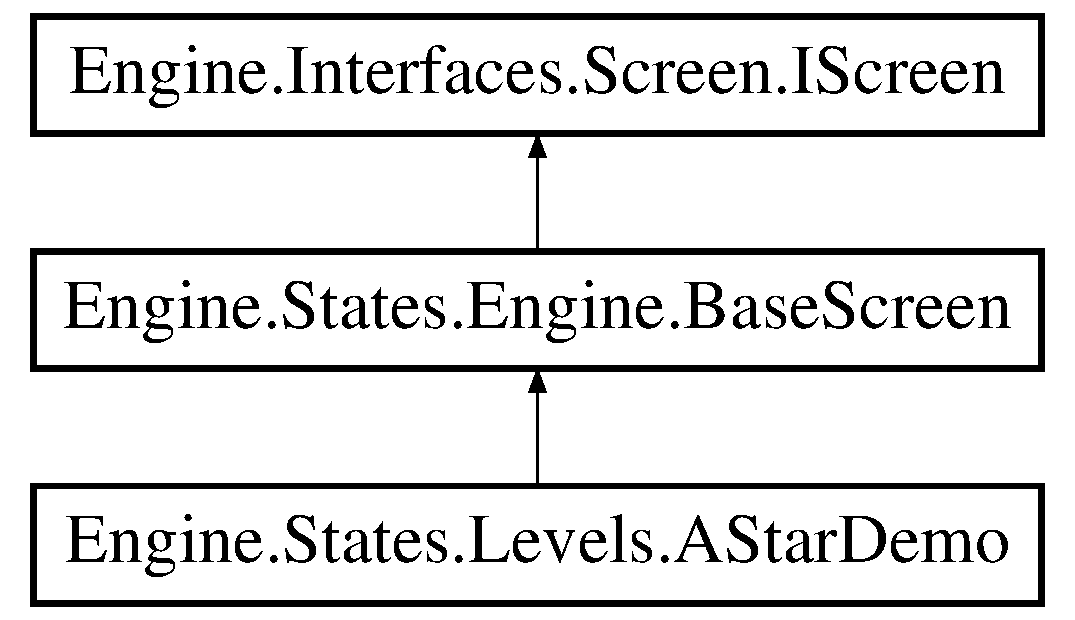
\includegraphics[height=3.000000cm]{d3/d2f/a00562}
\end{center}
\end{figure}
\subsection*{Public Member Functions}
\begin{DoxyCompactItemize}
\item 
override void \hyperlink{a00562_a143dfe5c81e8cd31fe6439aad1de00c6}{Initialize} ()
\begin{DoxyCompactList}\small\item\em M\+E\+T\+H\+OD\+: Initialises the logic of the screen \end{DoxyCompactList}\item 
override void \hyperlink{a00562_a25e822fbb0f806e84f05a26852c05593}{Unload} ()
\begin{DoxyCompactList}\small\item\em M\+E\+T\+H\+OD\+: When the screen is to be unloaded, clear any entities from the screen, remove the entities from the detection manager as well \end{DoxyCompactList}\item 
override void \hyperlink{a00562_aaa91f362f279bd5d226f49fb150f98e3}{Update} (Game\+Time game\+Time)
\begin{DoxyCompactList}\small\item\em M\+E\+T\+H\+OD\+: The update loop which is cycled through each frame \end{DoxyCompactList}\item 
override void \hyperlink{a00562_ad5b2061652982cb94e7c01c39f59a984}{Draw} (Sprite\+Batch sprite\+Batch)
\begin{DoxyCompactList}\small\item\em M\+E\+T\+H\+OD\+: Draws the content of the screen \end{DoxyCompactList}\end{DoxyCompactItemize}
\subsection*{Additional Inherited Members}


\subsection{Member Function Documentation}
\mbox{\Hypertarget{a00562_ad5b2061652982cb94e7c01c39f59a984}\label{a00562_ad5b2061652982cb94e7c01c39f59a984}} 
\index{Engine\+::\+States\+::\+Levels\+::\+A\+Star\+Demo@{Engine\+::\+States\+::\+Levels\+::\+A\+Star\+Demo}!Draw@{Draw}}
\index{Draw@{Draw}!Engine\+::\+States\+::\+Levels\+::\+A\+Star\+Demo@{Engine\+::\+States\+::\+Levels\+::\+A\+Star\+Demo}}
\subsubsection{\texorpdfstring{Draw()}{Draw()}}
{\footnotesize\ttfamily override void Engine.\+States.\+Levels.\+A\+Star\+Demo.\+Draw (\begin{DoxyParamCaption}\item[{Sprite\+Batch}]{sprite\+Batch }\end{DoxyParamCaption})\hspace{0.3cm}{\ttfamily [inline]}, {\ttfamily [virtual]}}



M\+E\+T\+H\+OD\+: Draws the content of the screen 


\begin{DoxyParams}{Parameters}
{\em sprite\+Batch} & the Monogame Sprite\+Batch\\
\hline
\end{DoxyParams}


Reimplemented from \hyperlink{a00550_a200c31954effe5fc060118607155fb16}{Engine.\+States.\+Engine.\+Base\+Screen}.

\mbox{\Hypertarget{a00562_a143dfe5c81e8cd31fe6439aad1de00c6}\label{a00562_a143dfe5c81e8cd31fe6439aad1de00c6}} 
\index{Engine\+::\+States\+::\+Levels\+::\+A\+Star\+Demo@{Engine\+::\+States\+::\+Levels\+::\+A\+Star\+Demo}!Initialize@{Initialize}}
\index{Initialize@{Initialize}!Engine\+::\+States\+::\+Levels\+::\+A\+Star\+Demo@{Engine\+::\+States\+::\+Levels\+::\+A\+Star\+Demo}}
\subsubsection{\texorpdfstring{Initialize()}{Initialize()}}
{\footnotesize\ttfamily override void Engine.\+States.\+Levels.\+A\+Star\+Demo.\+Initialize (\begin{DoxyParamCaption}{ }\end{DoxyParamCaption})\hspace{0.3cm}{\ttfamily [inline]}, {\ttfamily [virtual]}}



M\+E\+T\+H\+OD\+: Initialises the logic of the screen 



Reimplemented from \hyperlink{a00550_af8fd6890abf865641e190578ef2e054c}{Engine.\+States.\+Engine.\+Base\+Screen}.

\mbox{\Hypertarget{a00562_a25e822fbb0f806e84f05a26852c05593}\label{a00562_a25e822fbb0f806e84f05a26852c05593}} 
\index{Engine\+::\+States\+::\+Levels\+::\+A\+Star\+Demo@{Engine\+::\+States\+::\+Levels\+::\+A\+Star\+Demo}!Unload@{Unload}}
\index{Unload@{Unload}!Engine\+::\+States\+::\+Levels\+::\+A\+Star\+Demo@{Engine\+::\+States\+::\+Levels\+::\+A\+Star\+Demo}}
\subsubsection{\texorpdfstring{Unload()}{Unload()}}
{\footnotesize\ttfamily override void Engine.\+States.\+Levels.\+A\+Star\+Demo.\+Unload (\begin{DoxyParamCaption}{ }\end{DoxyParamCaption})\hspace{0.3cm}{\ttfamily [inline]}, {\ttfamily [virtual]}}



M\+E\+T\+H\+OD\+: When the screen is to be unloaded, clear any entities from the screen, remove the entities from the detection manager as well 



Reimplemented from \hyperlink{a00550_a861ab6364e68e3e3b6b9718e34ba18a2}{Engine.\+States.\+Engine.\+Base\+Screen}.

\mbox{\Hypertarget{a00562_aaa91f362f279bd5d226f49fb150f98e3}\label{a00562_aaa91f362f279bd5d226f49fb150f98e3}} 
\index{Engine\+::\+States\+::\+Levels\+::\+A\+Star\+Demo@{Engine\+::\+States\+::\+Levels\+::\+A\+Star\+Demo}!Update@{Update}}
\index{Update@{Update}!Engine\+::\+States\+::\+Levels\+::\+A\+Star\+Demo@{Engine\+::\+States\+::\+Levels\+::\+A\+Star\+Demo}}
\subsubsection{\texorpdfstring{Update()}{Update()}}
{\footnotesize\ttfamily override void Engine.\+States.\+Levels.\+A\+Star\+Demo.\+Update (\begin{DoxyParamCaption}\item[{Game\+Time}]{game\+Time }\end{DoxyParamCaption})\hspace{0.3cm}{\ttfamily [inline]}, {\ttfamily [virtual]}}



M\+E\+T\+H\+OD\+: The update loop which is cycled through each frame 


\begin{DoxyParams}{Parameters}
{\em game\+Time} & the Monogame Game\+Time property\\
\hline
\end{DoxyParams}


Reimplemented from \hyperlink{a00550_a098ece7d1e112475f6e880c3a672af64}{Engine.\+States.\+Engine.\+Base\+Screen}.



The documentation for this class was generated from the following file\+:\begin{DoxyCompactItemize}
\item 
\hyperlink{a00203}{A\+Star\+Demo.\+cs}\end{DoxyCompactItemize}

\hypertarget{a00398}{}\section{Engine.\+Grid.\+A\+Star\+Grid\+Search Class Reference}
\label{a00398}\index{Engine.\+Grid.\+A\+Star\+Grid\+Search@{Engine.\+Grid.\+A\+Star\+Grid\+Search}}
\subsection*{Public Member Functions}
\begin{DoxyCompactItemize}
\item 
\hyperlink{a00398_a29a934525f624e8c6ee7693f04df61c0}{A\+Star\+Grid\+Search} (\hyperlink{a00406}{Grids} grid)
\item 
void \hyperlink{a00398_a9b15ad7367bb5421108a9232d4c4954c}{Search} (\hyperlink{a00414}{Node} p\+Start, \hyperlink{a00414}{Node} p\+Goal, Texture2D p\+Check)
\item 
void \hyperlink{a00398_a1d4e74e3564bffa81262c73e2ecfcdfc}{add\+Blocked} (int x, int y)
\item 
void \hyperlink{a00398_a0e6a0e9cbcdaccff905216da631fad56}{reset\+Walls} ()
\item 
void \hyperlink{a00398_a0376f68fb9f4d45d11be4855fece5e56}{Show} (\hyperlink{a00414}{Node} start, \hyperlink{a00414}{Node} end)
\item 
Queue$<$ \hyperlink{a00414}{Node} $>$ \hyperlink{a00398_a8d3cb5019defd8e526d0c1111bcf2986}{get\+Path} ()
\item 
List$<$ \hyperlink{a00414}{Node} $>$ \hyperlink{a00398_a47ea78e4c6a2d333de9373b62543cbc7}{get\+Pathv} ()
\end{DoxyCompactItemize}


\subsection{Constructor \& Destructor Documentation}
\mbox{\Hypertarget{a00398_a29a934525f624e8c6ee7693f04df61c0}\label{a00398_a29a934525f624e8c6ee7693f04df61c0}} 
\index{Engine\+::\+Grid\+::\+A\+Star\+Grid\+Search@{Engine\+::\+Grid\+::\+A\+Star\+Grid\+Search}!A\+Star\+Grid\+Search@{A\+Star\+Grid\+Search}}
\index{A\+Star\+Grid\+Search@{A\+Star\+Grid\+Search}!Engine\+::\+Grid\+::\+A\+Star\+Grid\+Search@{Engine\+::\+Grid\+::\+A\+Star\+Grid\+Search}}
\subsubsection{\texorpdfstring{A\+Star\+Grid\+Search()}{AStarGridSearch()}}
{\footnotesize\ttfamily Engine.\+Grid.\+A\+Star\+Grid\+Search.\+A\+Star\+Grid\+Search (\begin{DoxyParamCaption}\item[{\hyperlink{a00406}{Grids}}]{grid }\end{DoxyParamCaption})\hspace{0.3cm}{\ttfamily [inline]}}



\subsection{Member Function Documentation}
\mbox{\Hypertarget{a00398_a1d4e74e3564bffa81262c73e2ecfcdfc}\label{a00398_a1d4e74e3564bffa81262c73e2ecfcdfc}} 
\index{Engine\+::\+Grid\+::\+A\+Star\+Grid\+Search@{Engine\+::\+Grid\+::\+A\+Star\+Grid\+Search}!add\+Blocked@{add\+Blocked}}
\index{add\+Blocked@{add\+Blocked}!Engine\+::\+Grid\+::\+A\+Star\+Grid\+Search@{Engine\+::\+Grid\+::\+A\+Star\+Grid\+Search}}
\subsubsection{\texorpdfstring{add\+Blocked()}{addBlocked()}}
{\footnotesize\ttfamily void Engine.\+Grid.\+A\+Star\+Grid\+Search.\+add\+Blocked (\begin{DoxyParamCaption}\item[{int}]{x,  }\item[{int}]{y }\end{DoxyParamCaption})\hspace{0.3cm}{\ttfamily [inline]}}

\mbox{\Hypertarget{a00398_a8d3cb5019defd8e526d0c1111bcf2986}\label{a00398_a8d3cb5019defd8e526d0c1111bcf2986}} 
\index{Engine\+::\+Grid\+::\+A\+Star\+Grid\+Search@{Engine\+::\+Grid\+::\+A\+Star\+Grid\+Search}!get\+Path@{get\+Path}}
\index{get\+Path@{get\+Path}!Engine\+::\+Grid\+::\+A\+Star\+Grid\+Search@{Engine\+::\+Grid\+::\+A\+Star\+Grid\+Search}}
\subsubsection{\texorpdfstring{get\+Path()}{getPath()}}
{\footnotesize\ttfamily Queue$<$\hyperlink{a00414}{Node}$>$ Engine.\+Grid.\+A\+Star\+Grid\+Search.\+get\+Path (\begin{DoxyParamCaption}{ }\end{DoxyParamCaption})\hspace{0.3cm}{\ttfamily [inline]}}

\mbox{\Hypertarget{a00398_a47ea78e4c6a2d333de9373b62543cbc7}\label{a00398_a47ea78e4c6a2d333de9373b62543cbc7}} 
\index{Engine\+::\+Grid\+::\+A\+Star\+Grid\+Search@{Engine\+::\+Grid\+::\+A\+Star\+Grid\+Search}!get\+Pathv@{get\+Pathv}}
\index{get\+Pathv@{get\+Pathv}!Engine\+::\+Grid\+::\+A\+Star\+Grid\+Search@{Engine\+::\+Grid\+::\+A\+Star\+Grid\+Search}}
\subsubsection{\texorpdfstring{get\+Pathv()}{getPathv()}}
{\footnotesize\ttfamily List$<$\hyperlink{a00414}{Node}$>$ Engine.\+Grid.\+A\+Star\+Grid\+Search.\+get\+Pathv (\begin{DoxyParamCaption}{ }\end{DoxyParamCaption})\hspace{0.3cm}{\ttfamily [inline]}}

\mbox{\Hypertarget{a00398_a0e6a0e9cbcdaccff905216da631fad56}\label{a00398_a0e6a0e9cbcdaccff905216da631fad56}} 
\index{Engine\+::\+Grid\+::\+A\+Star\+Grid\+Search@{Engine\+::\+Grid\+::\+A\+Star\+Grid\+Search}!reset\+Walls@{reset\+Walls}}
\index{reset\+Walls@{reset\+Walls}!Engine\+::\+Grid\+::\+A\+Star\+Grid\+Search@{Engine\+::\+Grid\+::\+A\+Star\+Grid\+Search}}
\subsubsection{\texorpdfstring{reset\+Walls()}{resetWalls()}}
{\footnotesize\ttfamily void Engine.\+Grid.\+A\+Star\+Grid\+Search.\+reset\+Walls (\begin{DoxyParamCaption}{ }\end{DoxyParamCaption})\hspace{0.3cm}{\ttfamily [inline]}}

\mbox{\Hypertarget{a00398_a9b15ad7367bb5421108a9232d4c4954c}\label{a00398_a9b15ad7367bb5421108a9232d4c4954c}} 
\index{Engine\+::\+Grid\+::\+A\+Star\+Grid\+Search@{Engine\+::\+Grid\+::\+A\+Star\+Grid\+Search}!Search@{Search}}
\index{Search@{Search}!Engine\+::\+Grid\+::\+A\+Star\+Grid\+Search@{Engine\+::\+Grid\+::\+A\+Star\+Grid\+Search}}
\subsubsection{\texorpdfstring{Search()}{Search()}}
{\footnotesize\ttfamily void Engine.\+Grid.\+A\+Star\+Grid\+Search.\+Search (\begin{DoxyParamCaption}\item[{\hyperlink{a00414}{Node}}]{p\+Start,  }\item[{\hyperlink{a00414}{Node}}]{p\+Goal,  }\item[{Texture2D}]{p\+Check }\end{DoxyParamCaption})\hspace{0.3cm}{\ttfamily [inline]}}

Assign variables

start.\+G = get\+Distance(start, p\+Goal); Add the start node to the list for checking

Dont stop the search whilst there are nodes available or if the goal hasnt been found

Assign the current node of interest to the first open index

Find the fittest node around the current node and assign it

The node has been checked, move it from the open into the closed list

Check if we\textquotesingle{}ve found the goal

Stop the loop

Show\+Path(goal); start = current;

Draw the path. \mbox{\Hypertarget{a00398_a0376f68fb9f4d45d11be4855fece5e56}\label{a00398_a0376f68fb9f4d45d11be4855fece5e56}} 
\index{Engine\+::\+Grid\+::\+A\+Star\+Grid\+Search@{Engine\+::\+Grid\+::\+A\+Star\+Grid\+Search}!Show@{Show}}
\index{Show@{Show}!Engine\+::\+Grid\+::\+A\+Star\+Grid\+Search@{Engine\+::\+Grid\+::\+A\+Star\+Grid\+Search}}
\subsubsection{\texorpdfstring{Show()}{Show()}}
{\footnotesize\ttfamily void Engine.\+Grid.\+A\+Star\+Grid\+Search.\+Show (\begin{DoxyParamCaption}\item[{\hyperlink{a00414}{Node}}]{start,  }\item[{\hyperlink{a00414}{Node}}]{end }\end{DoxyParamCaption})\hspace{0.3cm}{\ttfamily [inline]}}

Set the last node to be checked first so we can retrace the path back

Dont draw on the start node

Add all nodes inbetween

Set up the link to loop back with (The parent node is the previous closest node that was checked and added to the open list)

Little method I added to remove goal node since I hvent had much luck

Let the grid know of the path to draw it $<$$<$ change 

The documentation for this class was generated from the following file\+:\begin{DoxyCompactItemize}
\item 
\hyperlink{a00080}{A\+Star\+Grid\+Search.\+cs}\end{DoxyCompactItemize}

\hypertarget{a00402}{}\section{Engine.\+Grid.\+A\+Star\+Node Class Reference}
\label{a00402}\index{Engine.\+Grid.\+A\+Star\+Node@{Engine.\+Grid.\+A\+Star\+Node}}
\subsection*{Public Member Functions}
\begin{DoxyCompactItemize}
\item 
\hyperlink{a00402_a7a3c8e3fd948f9d8cc3b54785ee158fd}{A\+Star\+Node} (int element, string tex)
\item 
\hyperlink{a00402_aa1178655cad381caac040bf8da0a31e0}{A\+Star\+Node} (int element)
\item 
void \hyperlink{a00402_a466f4f5a7adfb5bfcacc1289c777c477}{Draw} (Sprite\+Batch sp)
\end{DoxyCompactItemize}
\subsection*{Properties}
\begin{DoxyCompactItemize}
\item 
int \hyperlink{a00402_a6579e5c7fd60346c98cead260791ad77}{G}\hspace{0.3cm}{\ttfamily  \mbox{[}get, set\mbox{]}}
\item 
int \hyperlink{a00402_ac65eea2ee92b33d7afde19dc0b94dbea}{H}\hspace{0.3cm}{\ttfamily  \mbox{[}get, set\mbox{]}}
\item 
int \hyperlink{a00402_aab3ff45feb87f3f6f86bbc6ba1661fb8}{F}\hspace{0.3cm}{\ttfamily  \mbox{[}get\mbox{]}}
\end{DoxyCompactItemize}


\subsection{Constructor \& Destructor Documentation}
\mbox{\Hypertarget{a00402_a7a3c8e3fd948f9d8cc3b54785ee158fd}\label{a00402_a7a3c8e3fd948f9d8cc3b54785ee158fd}} 
\index{Engine\+::\+Grid\+::\+A\+Star\+Node@{Engine\+::\+Grid\+::\+A\+Star\+Node}!A\+Star\+Node@{A\+Star\+Node}}
\index{A\+Star\+Node@{A\+Star\+Node}!Engine\+::\+Grid\+::\+A\+Star\+Node@{Engine\+::\+Grid\+::\+A\+Star\+Node}}
\subsubsection{\texorpdfstring{A\+Star\+Node()}{AStarNode()}\hspace{0.1cm}{\footnotesize\ttfamily [1/2]}}
{\footnotesize\ttfamily Engine.\+Grid.\+A\+Star\+Node.\+A\+Star\+Node (\begin{DoxyParamCaption}\item[{int}]{element,  }\item[{string}]{tex }\end{DoxyParamCaption})\hspace{0.3cm}{\ttfamily [inline]}}

\mbox{\Hypertarget{a00402_aa1178655cad381caac040bf8da0a31e0}\label{a00402_aa1178655cad381caac040bf8da0a31e0}} 
\index{Engine\+::\+Grid\+::\+A\+Star\+Node@{Engine\+::\+Grid\+::\+A\+Star\+Node}!A\+Star\+Node@{A\+Star\+Node}}
\index{A\+Star\+Node@{A\+Star\+Node}!Engine\+::\+Grid\+::\+A\+Star\+Node@{Engine\+::\+Grid\+::\+A\+Star\+Node}}
\subsubsection{\texorpdfstring{A\+Star\+Node()}{AStarNode()}\hspace{0.1cm}{\footnotesize\ttfamily [2/2]}}
{\footnotesize\ttfamily Engine.\+Grid.\+A\+Star\+Node.\+A\+Star\+Node (\begin{DoxyParamCaption}\item[{int}]{element }\end{DoxyParamCaption})\hspace{0.3cm}{\ttfamily [inline]}}



\subsection{Member Function Documentation}
\mbox{\Hypertarget{a00402_a466f4f5a7adfb5bfcacc1289c777c477}\label{a00402_a466f4f5a7adfb5bfcacc1289c777c477}} 
\index{Engine\+::\+Grid\+::\+A\+Star\+Node@{Engine\+::\+Grid\+::\+A\+Star\+Node}!Draw@{Draw}}
\index{Draw@{Draw}!Engine\+::\+Grid\+::\+A\+Star\+Node@{Engine\+::\+Grid\+::\+A\+Star\+Node}}
\subsubsection{\texorpdfstring{Draw()}{Draw()}}
{\footnotesize\ttfamily void Engine.\+Grid.\+A\+Star\+Node.\+Draw (\begin{DoxyParamCaption}\item[{Sprite\+Batch}]{sp }\end{DoxyParamCaption})\hspace{0.3cm}{\ttfamily [inline]}}



\subsection{Property Documentation}
\mbox{\Hypertarget{a00402_aab3ff45feb87f3f6f86bbc6ba1661fb8}\label{a00402_aab3ff45feb87f3f6f86bbc6ba1661fb8}} 
\index{Engine\+::\+Grid\+::\+A\+Star\+Node@{Engine\+::\+Grid\+::\+A\+Star\+Node}!F@{F}}
\index{F@{F}!Engine\+::\+Grid\+::\+A\+Star\+Node@{Engine\+::\+Grid\+::\+A\+Star\+Node}}
\subsubsection{\texorpdfstring{F}{F}}
{\footnotesize\ttfamily int Engine.\+Grid.\+A\+Star\+Node.\+F\hspace{0.3cm}{\ttfamily [get]}}

\mbox{\Hypertarget{a00402_a6579e5c7fd60346c98cead260791ad77}\label{a00402_a6579e5c7fd60346c98cead260791ad77}} 
\index{Engine\+::\+Grid\+::\+A\+Star\+Node@{Engine\+::\+Grid\+::\+A\+Star\+Node}!G@{G}}
\index{G@{G}!Engine\+::\+Grid\+::\+A\+Star\+Node@{Engine\+::\+Grid\+::\+A\+Star\+Node}}
\subsubsection{\texorpdfstring{G}{G}}
{\footnotesize\ttfamily int Engine.\+Grid.\+A\+Star\+Node.\+G\hspace{0.3cm}{\ttfamily [get]}, {\ttfamily [set]}}

\mbox{\Hypertarget{a00402_ac65eea2ee92b33d7afde19dc0b94dbea}\label{a00402_ac65eea2ee92b33d7afde19dc0b94dbea}} 
\index{Engine\+::\+Grid\+::\+A\+Star\+Node@{Engine\+::\+Grid\+::\+A\+Star\+Node}!H@{H}}
\index{H@{H}!Engine\+::\+Grid\+::\+A\+Star\+Node@{Engine\+::\+Grid\+::\+A\+Star\+Node}}
\subsubsection{\texorpdfstring{H}{H}}
{\footnotesize\ttfamily int Engine.\+Grid.\+A\+Star\+Node.\+H\hspace{0.3cm}{\ttfamily [get]}, {\ttfamily [set]}}



The documentation for this class was generated from the following file\+:\begin{DoxyCompactItemize}
\item 
\hyperlink{a00083}{A\+Star\+Node.\+cs}\end{DoxyCompactItemize}

\hypertarget{a00310}{}\section{Engine.\+Managers.\+A\+Star.\+Astar\+Path Class Reference}
\label{a00310}\index{Engine.\+Managers.\+A\+Star.\+Astar\+Path@{Engine.\+Managers.\+A\+Star.\+Astar\+Path}}
\subsection*{Public Member Functions}
\begin{DoxyCompactItemize}
\item 
void \hyperlink{a00310_a9912ab7f4be1ca36bc9b7e7081c5dd86}{Debug\+Path} ()
\begin{DoxyCompactList}\small\item\em M\+E\+T\+H\+OD\+: Show the debug path \end{DoxyCompactList}\item 
List$<$ \hyperlink{a00414}{Node} $>$ \hyperlink{a00310_aaa05e962c6e833ff7e22c4611ee492c7}{Commit\+Path\+Search} (\hyperlink{a00406}{Grids} grid, \hyperlink{a00414}{Node} Start, \hyperlink{a00414}{Node} Goal)
\begin{DoxyCompactList}\small\item\em M\+E\+T\+H\+OD\+: Commit a search and if it is successful, R\+E\+T\+U\+RN a list of nodes in the path \end{DoxyCompactList}\item 
Queue$<$ \hyperlink{a00414}{Node} $>$ \hyperlink{a00310_a1d55b6294c95c398017c25655bc4604f}{Commit\+Way\+Point\+Search} (\hyperlink{a00406}{Grids} grid, \hyperlink{a00414}{Node} Start, \hyperlink{a00414}{Node} Goal)
\begin{DoxyCompactList}\small\item\em M\+E\+T\+H\+OD\+: Commit a search and if it is successful, R\+E\+T\+U\+RN a queue of nodes in the path \end{DoxyCompactList}\end{DoxyCompactItemize}


\subsection{Member Function Documentation}
\mbox{\Hypertarget{a00310_aaa05e962c6e833ff7e22c4611ee492c7}\label{a00310_aaa05e962c6e833ff7e22c4611ee492c7}} 
\index{Engine\+::\+Managers\+::\+A\+Star\+::\+Astar\+Path@{Engine\+::\+Managers\+::\+A\+Star\+::\+Astar\+Path}!Commit\+Path\+Search@{Commit\+Path\+Search}}
\index{Commit\+Path\+Search@{Commit\+Path\+Search}!Engine\+::\+Managers\+::\+A\+Star\+::\+Astar\+Path@{Engine\+::\+Managers\+::\+A\+Star\+::\+Astar\+Path}}
\subsubsection{\texorpdfstring{Commit\+Path\+Search()}{CommitPathSearch()}}
{\footnotesize\ttfamily List$<$\hyperlink{a00414}{Node}$>$ Engine.\+Managers.\+A\+Star.\+Astar\+Path.\+Commit\+Path\+Search (\begin{DoxyParamCaption}\item[{\hyperlink{a00406}{Grids}}]{grid,  }\item[{\hyperlink{a00414}{Node}}]{Start,  }\item[{\hyperlink{a00414}{Node}}]{Goal }\end{DoxyParamCaption})\hspace{0.3cm}{\ttfamily [inline]}}



M\+E\+T\+H\+OD\+: Commit a search and if it is successful, R\+E\+T\+U\+RN a list of nodes in the path 


\begin{DoxyParams}{Parameters}
{\em grid} & \\
\hline
{\em Start} & \\
\hline
{\em Goal} & \\
\hline
\end{DoxyParams}
\begin{DoxyReturn}{Returns}

\end{DoxyReturn}
\mbox{\Hypertarget{a00310_a1d55b6294c95c398017c25655bc4604f}\label{a00310_a1d55b6294c95c398017c25655bc4604f}} 
\index{Engine\+::\+Managers\+::\+A\+Star\+::\+Astar\+Path@{Engine\+::\+Managers\+::\+A\+Star\+::\+Astar\+Path}!Commit\+Way\+Point\+Search@{Commit\+Way\+Point\+Search}}
\index{Commit\+Way\+Point\+Search@{Commit\+Way\+Point\+Search}!Engine\+::\+Managers\+::\+A\+Star\+::\+Astar\+Path@{Engine\+::\+Managers\+::\+A\+Star\+::\+Astar\+Path}}
\subsubsection{\texorpdfstring{Commit\+Way\+Point\+Search()}{CommitWayPointSearch()}}
{\footnotesize\ttfamily Queue$<$\hyperlink{a00414}{Node}$>$ Engine.\+Managers.\+A\+Star.\+Astar\+Path.\+Commit\+Way\+Point\+Search (\begin{DoxyParamCaption}\item[{\hyperlink{a00406}{Grids}}]{grid,  }\item[{\hyperlink{a00414}{Node}}]{Start,  }\item[{\hyperlink{a00414}{Node}}]{Goal }\end{DoxyParamCaption})\hspace{0.3cm}{\ttfamily [inline]}}



M\+E\+T\+H\+OD\+: Commit a search and if it is successful, R\+E\+T\+U\+RN a queue of nodes in the path 


\begin{DoxyParams}{Parameters}
{\em grid} & \\
\hline
{\em Start} & \\
\hline
{\em Goal} & \\
\hline
\end{DoxyParams}
\begin{DoxyReturn}{Returns}

\end{DoxyReturn}
\mbox{\Hypertarget{a00310_a9912ab7f4be1ca36bc9b7e7081c5dd86}\label{a00310_a9912ab7f4be1ca36bc9b7e7081c5dd86}} 
\index{Engine\+::\+Managers\+::\+A\+Star\+::\+Astar\+Path@{Engine\+::\+Managers\+::\+A\+Star\+::\+Astar\+Path}!Debug\+Path@{Debug\+Path}}
\index{Debug\+Path@{Debug\+Path}!Engine\+::\+Managers\+::\+A\+Star\+::\+Astar\+Path@{Engine\+::\+Managers\+::\+A\+Star\+::\+Astar\+Path}}
\subsubsection{\texorpdfstring{Debug\+Path()}{DebugPath()}}
{\footnotesize\ttfamily void Engine.\+Managers.\+A\+Star.\+Astar\+Path.\+Debug\+Path (\begin{DoxyParamCaption}{ }\end{DoxyParamCaption})\hspace{0.3cm}{\ttfamily [inline]}}



M\+E\+T\+H\+OD\+: Show the debug path 



The documentation for this class was generated from the following file\+:\begin{DoxyCompactItemize}
\item 
\hyperlink{a00014}{Astar\+Path.\+cs}\end{DoxyCompactItemize}

\hypertarget{a00550}{}\section{Engine.\+States.\+Engine.\+Base\+Screen Class Reference}
\label{a00550}\index{Engine.\+States.\+Engine.\+Base\+Screen@{Engine.\+States.\+Engine.\+Base\+Screen}}
Inheritance diagram for Engine.\+States.\+Engine.\+Base\+Screen\+:\begin{figure}[H]
\begin{center}
\leavevmode
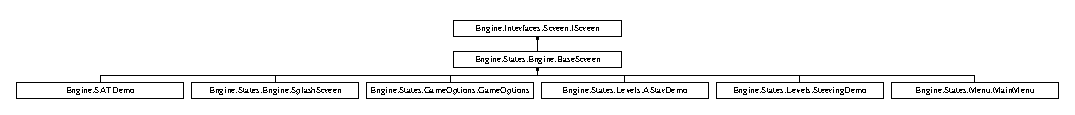
\includegraphics[height=1.098039cm]{de/de7/a00550}
\end{center}
\end{figure}
\subsection*{Public Member Functions}
\begin{DoxyCompactItemize}
\item 
\hyperlink{a00550_af66e62ec831d9ac03c231265b808417f}{Base\+Screen} ()
\begin{DoxyCompactList}\small\item\em C\+O\+N\+S\+T\+R\+U\+C\+T\+OR\+: \end{DoxyCompactList}\item 
virtual void \hyperlink{a00550_af8fd6890abf865641e190578ef2e054c}{Initialize} ()
\begin{DoxyCompactList}\small\item\em M\+E\+T\+H\+OD\+: Initialises the logic of the screen \end{DoxyCompactList}\item 
virtual void \hyperlink{a00550_abd2118fc928f9057ddacbe758b80fe68}{Unload\+Content} ()
\begin{DoxyCompactList}\small\item\em M\+E\+T\+H\+OD\+: Unload the screen \end{DoxyCompactList}\item 
virtual void \hyperlink{a00550_a098ece7d1e112475f6e880c3a672af64}{Update} (Game\+Time game\+Time)
\begin{DoxyCompactList}\small\item\em M\+E\+T\+H\+OD\+: The update loop which is cycled through each frame \end{DoxyCompactList}\item 
virtual void \hyperlink{a00550_a200c31954effe5fc060118607155fb16}{Draw} (Sprite\+Batch sprite\+Batch)
\begin{DoxyCompactList}\small\item\em M\+E\+T\+H\+OD\+: Draws the content of the screen \end{DoxyCompactList}\item 
virtual void \hyperlink{a00550_a861ab6364e68e3e3b6b9718e34ba18a2}{Unload} ()
\begin{DoxyCompactList}\small\item\em M\+E\+T\+H\+OD\+: When the screen is to be unloaded, clear any entities from the screen, remove the entities from the detection manager as well \end{DoxyCompactList}\end{DoxyCompactItemize}
\subsection*{Properties}
\begin{DoxyCompactItemize}
\item 
bool \hyperlink{a00550_ac5d310a291bb741ffd071372bc1ba496}{Active}\hspace{0.3cm}{\ttfamily  \mbox{[}get, set\mbox{]}}
\begin{DoxyCompactList}\small\item\em G\+ET\+: S\+ET\+: bool for if screen is active screen \end{DoxyCompactList}\item 
string \hyperlink{a00550_af942c6eeee717dee53a460530f4efb3d}{Sound\+Track}\hspace{0.3cm}{\ttfamily  \mbox{[}get, set\mbox{]}}
\begin{DoxyCompactList}\small\item\em G\+ET\+: S\+ET\+: Does the screen have a soundtrack \end{DoxyCompactList}\end{DoxyCompactItemize}


\subsection{Constructor \& Destructor Documentation}
\mbox{\Hypertarget{a00550_af66e62ec831d9ac03c231265b808417f}\label{a00550_af66e62ec831d9ac03c231265b808417f}} 
\index{Engine\+::\+States\+::\+Engine\+::\+Base\+Screen@{Engine\+::\+States\+::\+Engine\+::\+Base\+Screen}!Base\+Screen@{Base\+Screen}}
\index{Base\+Screen@{Base\+Screen}!Engine\+::\+States\+::\+Engine\+::\+Base\+Screen@{Engine\+::\+States\+::\+Engine\+::\+Base\+Screen}}
\subsubsection{\texorpdfstring{Base\+Screen()}{BaseScreen()}}
{\footnotesize\ttfamily Engine.\+States.\+Engine.\+Base\+Screen.\+Base\+Screen (\begin{DoxyParamCaption}{ }\end{DoxyParamCaption})\hspace{0.3cm}{\ttfamily [inline]}}



C\+O\+N\+S\+T\+R\+U\+C\+T\+OR\+: 



\subsection{Member Function Documentation}
\mbox{\Hypertarget{a00550_a200c31954effe5fc060118607155fb16}\label{a00550_a200c31954effe5fc060118607155fb16}} 
\index{Engine\+::\+States\+::\+Engine\+::\+Base\+Screen@{Engine\+::\+States\+::\+Engine\+::\+Base\+Screen}!Draw@{Draw}}
\index{Draw@{Draw}!Engine\+::\+States\+::\+Engine\+::\+Base\+Screen@{Engine\+::\+States\+::\+Engine\+::\+Base\+Screen}}
\subsubsection{\texorpdfstring{Draw()}{Draw()}}
{\footnotesize\ttfamily virtual void Engine.\+States.\+Engine.\+Base\+Screen.\+Draw (\begin{DoxyParamCaption}\item[{Sprite\+Batch}]{sprite\+Batch }\end{DoxyParamCaption})\hspace{0.3cm}{\ttfamily [inline]}, {\ttfamily [virtual]}}



M\+E\+T\+H\+OD\+: Draws the content of the screen 


\begin{DoxyParams}{Parameters}
{\em sprite\+Batch} & the Monogame Sprite\+Batch\\
\hline
\end{DoxyParams}


Implements \hyperlink{a00466_a0c61f739fb252fcc90b91b1358511d05}{Engine.\+Interfaces.\+Screen.\+I\+Screen}.



Reimplemented in \hyperlink{a00562_ad5b2061652982cb94e7c01c39f59a984}{Engine.\+States.\+Levels.\+A\+Star\+Demo}, \hyperlink{a00574_a193970cc59914f538ae0bcd39fe1ef48}{Engine.\+States.\+Menu.\+Main\+Menu}, \hyperlink{a00570_a32c772a646fe78f26a4e9f83ae327156}{Engine.\+States.\+Levels.\+Steering\+Demo}, and \hyperlink{a00554_ae50fb213e5c1efc8d3908340b236e927}{Engine.\+States.\+Engine.\+Splash\+Screen}.

\mbox{\Hypertarget{a00550_af8fd6890abf865641e190578ef2e054c}\label{a00550_af8fd6890abf865641e190578ef2e054c}} 
\index{Engine\+::\+States\+::\+Engine\+::\+Base\+Screen@{Engine\+::\+States\+::\+Engine\+::\+Base\+Screen}!Initialize@{Initialize}}
\index{Initialize@{Initialize}!Engine\+::\+States\+::\+Engine\+::\+Base\+Screen@{Engine\+::\+States\+::\+Engine\+::\+Base\+Screen}}
\subsubsection{\texorpdfstring{Initialize()}{Initialize()}}
{\footnotesize\ttfamily virtual void Engine.\+States.\+Engine.\+Base\+Screen.\+Initialize (\begin{DoxyParamCaption}{ }\end{DoxyParamCaption})\hspace{0.3cm}{\ttfamily [inline]}, {\ttfamily [virtual]}}



M\+E\+T\+H\+OD\+: Initialises the logic of the screen 



Implements \hyperlink{a00466_ad251ad712685a0f329ad2b29bde78981}{Engine.\+Interfaces.\+Screen.\+I\+Screen}.



Reimplemented in \hyperlink{a00558_a1547a699546baa41aa39a2e2b4412787}{Engine.\+States.\+Game\+Options.\+Game\+Options}, \hyperlink{a00574_a43b83f0941e721234fdceeb0b5587f1b}{Engine.\+States.\+Menu.\+Main\+Menu}, \hyperlink{a00554_a321c34cdc158a49cf76f31e3cdd0863e}{Engine.\+States.\+Engine.\+Splash\+Screen}, \hyperlink{a00562_a143dfe5c81e8cd31fe6439aad1de00c6}{Engine.\+States.\+Levels.\+A\+Star\+Demo}, \hyperlink{a00570_a3ae8b73b4618e8c2635d3b8c24d70bcb}{Engine.\+States.\+Levels.\+Steering\+Demo}, and \hyperlink{a00566_a051d8aea070a4c7a93f0cf494e4fac6a}{Engine.\+S\+A\+T\+Demo}.

\mbox{\Hypertarget{a00550_a861ab6364e68e3e3b6b9718e34ba18a2}\label{a00550_a861ab6364e68e3e3b6b9718e34ba18a2}} 
\index{Engine\+::\+States\+::\+Engine\+::\+Base\+Screen@{Engine\+::\+States\+::\+Engine\+::\+Base\+Screen}!Unload@{Unload}}
\index{Unload@{Unload}!Engine\+::\+States\+::\+Engine\+::\+Base\+Screen@{Engine\+::\+States\+::\+Engine\+::\+Base\+Screen}}
\subsubsection{\texorpdfstring{Unload()}{Unload()}}
{\footnotesize\ttfamily virtual void Engine.\+States.\+Engine.\+Base\+Screen.\+Unload (\begin{DoxyParamCaption}{ }\end{DoxyParamCaption})\hspace{0.3cm}{\ttfamily [inline]}, {\ttfamily [virtual]}}



M\+E\+T\+H\+OD\+: When the screen is to be unloaded, clear any entities from the screen, remove the entities from the detection manager as well 



Implements \hyperlink{a00466_a67f1b5deb3604a417d7452fc8873de37}{Engine.\+Interfaces.\+Screen.\+I\+Screen}.



Reimplemented in \hyperlink{a00558_aedf1c1415b77bf7c8ce37d754039de7b}{Engine.\+States.\+Game\+Options.\+Game\+Options}, and \hyperlink{a00562_a25e822fbb0f806e84f05a26852c05593}{Engine.\+States.\+Levels.\+A\+Star\+Demo}.

\mbox{\Hypertarget{a00550_abd2118fc928f9057ddacbe758b80fe68}\label{a00550_abd2118fc928f9057ddacbe758b80fe68}} 
\index{Engine\+::\+States\+::\+Engine\+::\+Base\+Screen@{Engine\+::\+States\+::\+Engine\+::\+Base\+Screen}!Unload\+Content@{Unload\+Content}}
\index{Unload\+Content@{Unload\+Content}!Engine\+::\+States\+::\+Engine\+::\+Base\+Screen@{Engine\+::\+States\+::\+Engine\+::\+Base\+Screen}}
\subsubsection{\texorpdfstring{Unload\+Content()}{UnloadContent()}}
{\footnotesize\ttfamily virtual void Engine.\+States.\+Engine.\+Base\+Screen.\+Unload\+Content (\begin{DoxyParamCaption}{ }\end{DoxyParamCaption})\hspace{0.3cm}{\ttfamily [inline]}, {\ttfamily [virtual]}}



M\+E\+T\+H\+OD\+: Unload the screen 



Implements \hyperlink{a00466_aeba867b4e4bd2f0a918b837d93a4e45a}{Engine.\+Interfaces.\+Screen.\+I\+Screen}.

\mbox{\Hypertarget{a00550_a098ece7d1e112475f6e880c3a672af64}\label{a00550_a098ece7d1e112475f6e880c3a672af64}} 
\index{Engine\+::\+States\+::\+Engine\+::\+Base\+Screen@{Engine\+::\+States\+::\+Engine\+::\+Base\+Screen}!Update@{Update}}
\index{Update@{Update}!Engine\+::\+States\+::\+Engine\+::\+Base\+Screen@{Engine\+::\+States\+::\+Engine\+::\+Base\+Screen}}
\subsubsection{\texorpdfstring{Update()}{Update()}}
{\footnotesize\ttfamily virtual void Engine.\+States.\+Engine.\+Base\+Screen.\+Update (\begin{DoxyParamCaption}\item[{Game\+Time}]{game\+Time }\end{DoxyParamCaption})\hspace{0.3cm}{\ttfamily [inline]}, {\ttfamily [virtual]}}



M\+E\+T\+H\+OD\+: The update loop which is cycled through each frame 


\begin{DoxyParams}{Parameters}
{\em game\+Time} & the Monogame Game\+Time property\\
\hline
\end{DoxyParams}


Implements \hyperlink{a00466_a5f59b9b12c1bf29b1db612ed52d1cfd6}{Engine.\+Interfaces.\+Screen.\+I\+Screen}.



Reimplemented in \hyperlink{a00558_a629d2a00abd6bfcc21524911e74fee3a}{Engine.\+States.\+Game\+Options.\+Game\+Options}, \hyperlink{a00574_ad667a7ff9dea79bee26a4205418c7a61}{Engine.\+States.\+Menu.\+Main\+Menu}, \hyperlink{a00562_aaa91f362f279bd5d226f49fb150f98e3}{Engine.\+States.\+Levels.\+A\+Star\+Demo}, \hyperlink{a00554_af245506899484c6784a44550b1364b6c}{Engine.\+States.\+Engine.\+Splash\+Screen}, and \hyperlink{a00570_a4210cc45e9038a007132fbafde08fa71}{Engine.\+States.\+Levels.\+Steering\+Demo}.



\subsection{Property Documentation}
\mbox{\Hypertarget{a00550_ac5d310a291bb741ffd071372bc1ba496}\label{a00550_ac5d310a291bb741ffd071372bc1ba496}} 
\index{Engine\+::\+States\+::\+Engine\+::\+Base\+Screen@{Engine\+::\+States\+::\+Engine\+::\+Base\+Screen}!Active@{Active}}
\index{Active@{Active}!Engine\+::\+States\+::\+Engine\+::\+Base\+Screen@{Engine\+::\+States\+::\+Engine\+::\+Base\+Screen}}
\subsubsection{\texorpdfstring{Active}{Active}}
{\footnotesize\ttfamily bool Engine.\+States.\+Engine.\+Base\+Screen.\+Active\hspace{0.3cm}{\ttfamily [get]}, {\ttfamily [set]}}



G\+ET\+: S\+ET\+: bool for if screen is active screen 

\mbox{\Hypertarget{a00550_af942c6eeee717dee53a460530f4efb3d}\label{a00550_af942c6eeee717dee53a460530f4efb3d}} 
\index{Engine\+::\+States\+::\+Engine\+::\+Base\+Screen@{Engine\+::\+States\+::\+Engine\+::\+Base\+Screen}!Sound\+Track@{Sound\+Track}}
\index{Sound\+Track@{Sound\+Track}!Engine\+::\+States\+::\+Engine\+::\+Base\+Screen@{Engine\+::\+States\+::\+Engine\+::\+Base\+Screen}}
\subsubsection{\texorpdfstring{Sound\+Track}{SoundTrack}}
{\footnotesize\ttfamily string Engine.\+States.\+Engine.\+Base\+Screen.\+Sound\+Track\hspace{0.3cm}{\ttfamily [get]}, {\ttfamily [set]}}



G\+ET\+: S\+ET\+: Does the screen have a soundtrack 



The documentation for this class was generated from the following file\+:\begin{DoxyCompactItemize}
\item 
\hyperlink{a00194}{Base\+Screen.\+cs}\end{DoxyCompactItemize}

\hypertarget{a00486}{}\section{Engine.\+Managers.\+Behaviour.\+Behaviour\+Manager Class Reference}
\label{a00486}\index{Engine.\+Managers.\+Behaviour.\+Behaviour\+Manager@{Engine.\+Managers.\+Behaviour.\+Behaviour\+Manager}}
Inheritance diagram for Engine.\+Managers.\+Behaviour.\+Behaviour\+Manager\+:\begin{figure}[H]
\begin{center}
\leavevmode
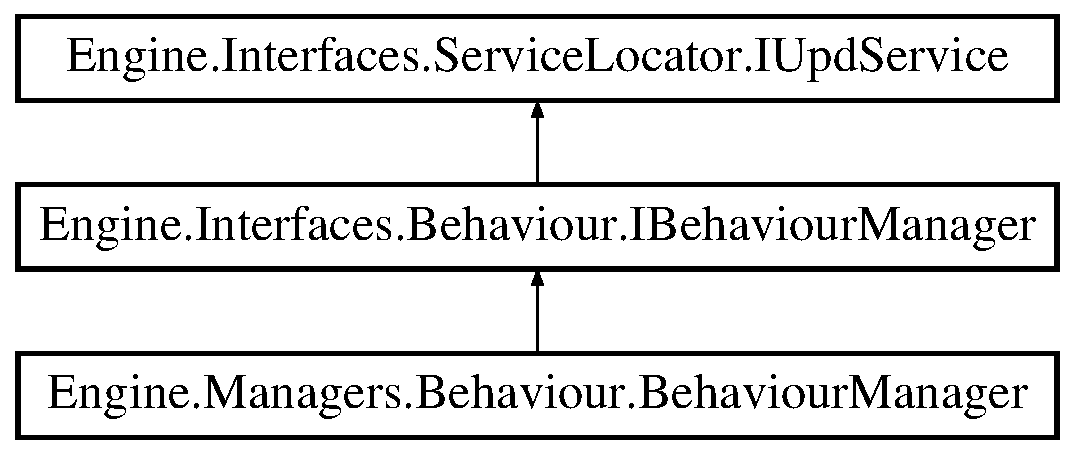
\includegraphics[height=3.000000cm]{db/df1/a00486}
\end{center}
\end{figure}
\subsection*{Public Member Functions}
\begin{DoxyCompactItemize}
\item 
\hyperlink{a00446}{I\+Mind} \hyperlink{a00486_a13eea511ff6d2cdeb8287b63034ce898}{Create$<$ T $>$} (\hyperlink{a00438}{I\+Entity} ie)
\begin{DoxyCompactList}\small\item\em M\+E\+T\+H\+OD\+: Create a new I\+Mind of type T \end{DoxyCompactList}\item 
void \hyperlink{a00486_ae21fe19ea423236e26d4f022230a071e}{clear\+List} ()
\begin{DoxyCompactList}\small\item\em M\+E\+T\+H\+OD\+: Clears the current list of all minds \end{DoxyCompactList}\item 
void \hyperlink{a00486_a684853fb49121d19f4d5c635153b871a}{remove\+Mind} (int id)
\begin{DoxyCompactList}\small\item\em M\+E\+T\+H\+OD\+: Removes a specific mind from the list based on the id provided \end{DoxyCompactList}\item 
\hyperlink{a00446}{I\+Mind} \hyperlink{a00486_a4391a84eadd13a812977cd51e177e00b}{get\+Mind} (int id)
\begin{DoxyCompactList}\small\item\em M\+E\+T\+H\+OD\+: Finds the mind in the list of the id provided \end{DoxyCompactList}\item 
void \hyperlink{a00486_a729bf10d2469de0497d75dfadbf56506}{Update} (Game\+Time game\+Time)
\begin{DoxyCompactList}\small\item\em M\+E\+T\+H\+OD\+: The update loop which is cycled through ever frame \end{DoxyCompactList}\end{DoxyCompactItemize}


\subsection{Member Function Documentation}
\mbox{\Hypertarget{a00486_ae21fe19ea423236e26d4f022230a071e}\label{a00486_ae21fe19ea423236e26d4f022230a071e}} 
\index{Engine\+::\+Managers\+::\+Behaviour\+::\+Behaviour\+Manager@{Engine\+::\+Managers\+::\+Behaviour\+::\+Behaviour\+Manager}!clear\+List@{clear\+List}}
\index{clear\+List@{clear\+List}!Engine\+::\+Managers\+::\+Behaviour\+::\+Behaviour\+Manager@{Engine\+::\+Managers\+::\+Behaviour\+::\+Behaviour\+Manager}}
\subsubsection{\texorpdfstring{clear\+List()}{clearList()}}
{\footnotesize\ttfamily void Engine.\+Managers.\+Behaviour.\+Behaviour\+Manager.\+clear\+List (\begin{DoxyParamCaption}{ }\end{DoxyParamCaption})\hspace{0.3cm}{\ttfamily [inline]}}



M\+E\+T\+H\+OD\+: Clears the current list of all minds 

For every mind in the list

Remove each mind

Clear the list to ensure the garbage collector gets everything 

Implements \hyperlink{a00418_ae944227a75ab665c4140628279296580}{Engine.\+Interfaces.\+Behaviour.\+I\+Behaviour\+Manager}.

\mbox{\Hypertarget{a00486_a13eea511ff6d2cdeb8287b63034ce898}\label{a00486_a13eea511ff6d2cdeb8287b63034ce898}} 
\index{Engine\+::\+Managers\+::\+Behaviour\+::\+Behaviour\+Manager@{Engine\+::\+Managers\+::\+Behaviour\+::\+Behaviour\+Manager}!Create$<$ T $>$@{Create$<$ T $>$}}
\index{Create$<$ T $>$@{Create$<$ T $>$}!Engine\+::\+Managers\+::\+Behaviour\+::\+Behaviour\+Manager@{Engine\+::\+Managers\+::\+Behaviour\+::\+Behaviour\+Manager}}
\subsubsection{\texorpdfstring{Create$<$ T $>$()}{Create< T >()}}
{\footnotesize\ttfamily \hyperlink{a00446}{I\+Mind} Engine.\+Managers.\+Behaviour.\+Behaviour\+Manager.\+Create$<$ T $>$ (\begin{DoxyParamCaption}\item[{\hyperlink{a00438}{I\+Entity}}]{ie }\end{DoxyParamCaption})\hspace{0.3cm}{\ttfamily [inline]}}



M\+E\+T\+H\+OD\+: Create a new I\+Mind of type T 


\begin{DoxyTemplParams}{Template Parameters}
{\em T} & Generic type for the mind that will be created\\
\hline
\end{DoxyTemplParams}

\begin{DoxyParams}{Parameters}
{\em ie} & the Entity the mind will be linked to\\
\hline
\end{DoxyParams}
\begin{DoxyReturn}{Returns}
a brand new I\+Mind
\end{DoxyReturn}
Create a new mind

Link the mind to the entity it controls

Add the mind to the collision List in the \hyperlink{a00268}{Collision} manager.

Add the mind to the list of minds.

Return the mind 

Implements \hyperlink{a00418_ad821620edeb0239197446bf1c3c32ee3}{Engine.\+Interfaces.\+Behaviour.\+I\+Behaviour\+Manager}.

\begin{Desc}
\item[Type Constraints]\begin{description}
\item[{\em T} : {\em I\+Mind}]\item[{\em T} : {\em new()}]\end{description}
\end{Desc}
\mbox{\Hypertarget{a00486_a4391a84eadd13a812977cd51e177e00b}\label{a00486_a4391a84eadd13a812977cd51e177e00b}} 
\index{Engine\+::\+Managers\+::\+Behaviour\+::\+Behaviour\+Manager@{Engine\+::\+Managers\+::\+Behaviour\+::\+Behaviour\+Manager}!get\+Mind@{get\+Mind}}
\index{get\+Mind@{get\+Mind}!Engine\+::\+Managers\+::\+Behaviour\+::\+Behaviour\+Manager@{Engine\+::\+Managers\+::\+Behaviour\+::\+Behaviour\+Manager}}
\subsubsection{\texorpdfstring{get\+Mind()}{getMind()}}
{\footnotesize\ttfamily \hyperlink{a00446}{I\+Mind} Engine.\+Managers.\+Behaviour.\+Behaviour\+Manager.\+get\+Mind (\begin{DoxyParamCaption}\item[{int}]{id }\end{DoxyParamCaption})\hspace{0.3cm}{\ttfamily [inline]}}



M\+E\+T\+H\+OD\+: Finds the mind in the list of the id provided 


\begin{DoxyParams}{Parameters}
{\em id} & the unique ID of the mind to be found\\
\hline
\end{DoxyParams}
\begin{DoxyReturn}{Returns}
an I\+Mind with the same unique ID
\end{DoxyReturn}
Every mind in the list of minds

If the id of this mind matches the parameter

Return this mind

If no mind has an ID matching we can return null 

Implements \hyperlink{a00418_ac1d24fb690a665ce8c70671b7c27b9ad}{Engine.\+Interfaces.\+Behaviour.\+I\+Behaviour\+Manager}.

\mbox{\Hypertarget{a00486_a684853fb49121d19f4d5c635153b871a}\label{a00486_a684853fb49121d19f4d5c635153b871a}} 
\index{Engine\+::\+Managers\+::\+Behaviour\+::\+Behaviour\+Manager@{Engine\+::\+Managers\+::\+Behaviour\+::\+Behaviour\+Manager}!remove\+Mind@{remove\+Mind}}
\index{remove\+Mind@{remove\+Mind}!Engine\+::\+Managers\+::\+Behaviour\+::\+Behaviour\+Manager@{Engine\+::\+Managers\+::\+Behaviour\+::\+Behaviour\+Manager}}
\subsubsection{\texorpdfstring{remove\+Mind()}{removeMind()}}
{\footnotesize\ttfamily void Engine.\+Managers.\+Behaviour.\+Behaviour\+Manager.\+remove\+Mind (\begin{DoxyParamCaption}\item[{int}]{id }\end{DoxyParamCaption})\hspace{0.3cm}{\ttfamily [inline]}}



M\+E\+T\+H\+OD\+: Removes a specific mind from the list based on the id provided 


\begin{DoxyParams}{Parameters}
{\em id} & the unique ID of the mind to be removed\\
\hline
\end{DoxyParams}
If the mind is out of the boundaries set remove it Temporary \hyperlink{a00266}{Behaviour} response. 

Implements \hyperlink{a00418_a6f89adf3a1d8286a73b534855847c414}{Engine.\+Interfaces.\+Behaviour.\+I\+Behaviour\+Manager}.

\mbox{\Hypertarget{a00486_a729bf10d2469de0497d75dfadbf56506}\label{a00486_a729bf10d2469de0497d75dfadbf56506}} 
\index{Engine\+::\+Managers\+::\+Behaviour\+::\+Behaviour\+Manager@{Engine\+::\+Managers\+::\+Behaviour\+::\+Behaviour\+Manager}!Update@{Update}}
\index{Update@{Update}!Engine\+::\+Managers\+::\+Behaviour\+::\+Behaviour\+Manager@{Engine\+::\+Managers\+::\+Behaviour\+::\+Behaviour\+Manager}}
\subsubsection{\texorpdfstring{Update()}{Update()}}
{\footnotesize\ttfamily void Engine.\+Managers.\+Behaviour.\+Behaviour\+Manager.\+Update (\begin{DoxyParamCaption}\item[{Game\+Time}]{game\+Time }\end{DoxyParamCaption})\hspace{0.3cm}{\ttfamily [inline]}}



M\+E\+T\+H\+OD\+: The update loop which is cycled through ever frame 


\begin{DoxyParams}{Parameters}
{\em game\+Time} & The Mono\+Game Gametime property\\
\hline
\end{DoxyParams}
For every mind in the list, run the Update method of each mind 

Implements \hyperlink{a00418_af161090c055167e2ca3901ed13d3d128}{Engine.\+Interfaces.\+Behaviour.\+I\+Behaviour\+Manager}.



The documentation for this class was generated from the following file\+:\begin{DoxyCompactItemize}
\item 
\hyperlink{a00146}{Behaviour\+Manager.\+cs}\end{DoxyCompactItemize}

\hypertarget{a00490}{}\section{Engine.\+Managers.\+Cam.\+Camera Class Reference}
\label{a00490}\index{Engine.\+Managers.\+Cam.\+Camera@{Engine.\+Managers.\+Cam.\+Camera}}
\subsection*{Public Member Functions}
\begin{DoxyCompactItemize}
\item 
\hyperlink{a00490_aa95d077fcb6779cf1d05dcd3924e47fd}{Camera} ()
\begin{DoxyCompactList}\small\item\em C\+O\+N\+S\+T\+R\+U\+C\+T\+OR \end{DoxyCompactList}\item 
void \hyperlink{a00490_aed786ac2b98679e90e3cc3fe5189f84e}{Move} (Vector2 amount)
\begin{DoxyCompactList}\small\item\em M\+E\+T\+H\+OD\+: Move the camera \end{DoxyCompactList}\item 
void \hyperlink{a00490_a7ba71eb9f006ab215b884763111c64f0}{set\+Entity} (\hyperlink{a00438}{I\+Entity} e, string Type)
\item 
Matrix \hyperlink{a00490_af3d0a20954c676fc8d14467fa6a3ed9f}{get\+\_\+transformation} (Graphics\+Device graphics\+Device)
\begin{DoxyCompactList}\small\item\em M\+E\+T\+H\+OD\+: Returns a matrix of the current transformation of the camera \end{DoxyCompactList}\item 
void \hyperlink{a00490_a40c128b7756087b2af6b3c3d62f83d08}{Update} ()
\item 
void \hyperlink{a00490_a77490f1a670ff106e843a46a712c9929}{check\+Possession} ()
\begin{DoxyCompactList}\small\item\em M\+E\+T\+H\+OD\+: Used to check if the camera is posessed by an object so that any move requests can be completed \end{DoxyCompactList}\item 
void \hyperlink{a00490_a93b217a61f0e87a0d184db27f7c0c1e7}{set\+Pos} (Vector2 pos)
\begin{DoxyCompactList}\small\item\em M\+E\+T\+H\+OD\+: Move the camera to a set position \end{DoxyCompactList}\item 
void \hyperlink{a00490_ae78f05538144a4613e5a601509482eea}{reset} ()
\item 
void \hyperlink{a00490_a87b553b3288448c4d6fe055398faa363}{check\+Input} ()
\end{DoxyCompactItemize}
\subsection*{Data Fields}
\begin{DoxyCompactItemize}
\item 
\hyperlink{a00267_aa40b88e1e953e36c54409ee9727c238b}{Camera\+Type} \hyperlink{a00490_a4394e674c32e8e3ca1b1fd25bc4277d4}{c\+Type}
\begin{DoxyCompactList}\small\item\em Used to determine the cameras behaviour. \end{DoxyCompactList}\item 
Matrix \hyperlink{a00490_a6760aa08917104a4c2937a9a7e05fe18}{\+\_\+transform}
\begin{DoxyCompactList}\small\item\em \hyperlink{a00490}{Camera} Zoom. \end{DoxyCompactList}\item 
Vector2 \hyperlink{a00490_a7b8a69cbcec7b5b8a463981970823b51}{\+\_\+pos}
\begin{DoxyCompactList}\small\item\em Matrix Transform. \end{DoxyCompactList}\end{DoxyCompactItemize}
\subsection*{Protected Attributes}
\begin{DoxyCompactItemize}
\item 
\hyperlink{a00438}{I\+Entity} \hyperlink{a00490_a2805d6ca57bb0d53772646539bb5fb71}{p}
\item 
float \hyperlink{a00490_a3909ab890f8c56d831d892bb6f6d4a20}{\+\_\+zoom}
\begin{DoxyCompactList}\small\item\em Target Entity. \end{DoxyCompactList}\item 
float \hyperlink{a00490_a34f440a1a9a332a065c4e022130d32dd}{\+\_\+rotation}
\begin{DoxyCompactList}\small\item\em \hyperlink{a00490}{Camera} Position. \end{DoxyCompactList}\item 
Vector2 \hyperlink{a00490_a44c44f9b99889984004062844ccbb23a}{\+\_\+o\+Pos}
\begin{DoxyCompactList}\small\item\em \hyperlink{a00490}{Camera} Rotation. \end{DoxyCompactList}\end{DoxyCompactItemize}
\subsection*{Properties}
\begin{DoxyCompactItemize}
\item 
float \hyperlink{a00490_a625deed885e044306674bce674f7ad52}{Zoom}\hspace{0.3cm}{\ttfamily  \mbox{[}get, set\mbox{]}}
\begin{DoxyCompactList}\small\item\em M\+E\+T\+H\+OD\+: Sets and gets zoom \end{DoxyCompactList}\item 
float \hyperlink{a00490_a18059d9071fd75793ceeee742c10e6bf}{Rotation}\hspace{0.3cm}{\ttfamily  \mbox{[}get, set\mbox{]}}
\begin{DoxyCompactList}\small\item\em G\+ET\+: S\+ET\+: Rotation \end{DoxyCompactList}\item 
Vector2 \hyperlink{a00490_acbd14e79831528efd53d6363f5a8a531}{Pos}\hspace{0.3cm}{\ttfamily  \mbox{[}get, set\mbox{]}}
\begin{DoxyCompactList}\small\item\em G\+ET\+: S\+ET\+: Position \end{DoxyCompactList}\end{DoxyCompactItemize}


\subsection{Constructor \& Destructor Documentation}
\mbox{\Hypertarget{a00490_aa95d077fcb6779cf1d05dcd3924e47fd}\label{a00490_aa95d077fcb6779cf1d05dcd3924e47fd}} 
\index{Engine\+::\+Managers\+::\+Cam\+::\+Camera@{Engine\+::\+Managers\+::\+Cam\+::\+Camera}!Camera@{Camera}}
\index{Camera@{Camera}!Engine\+::\+Managers\+::\+Cam\+::\+Camera@{Engine\+::\+Managers\+::\+Cam\+::\+Camera}}
\subsubsection{\texorpdfstring{Camera()}{Camera()}}
{\footnotesize\ttfamily Engine.\+Managers.\+Cam.\+Camera.\+Camera (\begin{DoxyParamCaption}{ }\end{DoxyParamCaption})\hspace{0.3cm}{\ttfamily [inline]}}



C\+O\+N\+S\+T\+R\+U\+C\+T\+OR 

Initalise the properties of the camera 

\subsection{Member Function Documentation}
\mbox{\Hypertarget{a00490_a87b553b3288448c4d6fe055398faa363}\label{a00490_a87b553b3288448c4d6fe055398faa363}} 
\index{Engine\+::\+Managers\+::\+Cam\+::\+Camera@{Engine\+::\+Managers\+::\+Cam\+::\+Camera}!check\+Input@{check\+Input}}
\index{check\+Input@{check\+Input}!Engine\+::\+Managers\+::\+Cam\+::\+Camera@{Engine\+::\+Managers\+::\+Cam\+::\+Camera}}
\subsubsection{\texorpdfstring{check\+Input()}{checkInput()}}
{\footnotesize\ttfamily void Engine.\+Managers.\+Cam.\+Camera.\+check\+Input (\begin{DoxyParamCaption}{ }\end{DoxyParamCaption})\hspace{0.3cm}{\ttfamily [inline]}}

If the L key is pressed then the camera is moved to match the zoom

If J is pressed then the camera is moved again

If I is pressed the camera is moved on the Y axis to match the zoom

Same as above but with K \mbox{\Hypertarget{a00490_a77490f1a670ff106e843a46a712c9929}\label{a00490_a77490f1a670ff106e843a46a712c9929}} 
\index{Engine\+::\+Managers\+::\+Cam\+::\+Camera@{Engine\+::\+Managers\+::\+Cam\+::\+Camera}!check\+Possession@{check\+Possession}}
\index{check\+Possession@{check\+Possession}!Engine\+::\+Managers\+::\+Cam\+::\+Camera@{Engine\+::\+Managers\+::\+Cam\+::\+Camera}}
\subsubsection{\texorpdfstring{check\+Possession()}{checkPossession()}}
{\footnotesize\ttfamily void Engine.\+Managers.\+Cam.\+Camera.\+check\+Possession (\begin{DoxyParamCaption}{ }\end{DoxyParamCaption})\hspace{0.3cm}{\ttfamily [inline]}}



M\+E\+T\+H\+OD\+: Used to check if the camera is posessed by an object so that any move requests can be completed 

If the camera is posessed

Follow the object that posesses the camera, usually this will be the player. \mbox{\Hypertarget{a00490_af3d0a20954c676fc8d14467fa6a3ed9f}\label{a00490_af3d0a20954c676fc8d14467fa6a3ed9f}} 
\index{Engine\+::\+Managers\+::\+Cam\+::\+Camera@{Engine\+::\+Managers\+::\+Cam\+::\+Camera}!get\+\_\+transformation@{get\+\_\+transformation}}
\index{get\+\_\+transformation@{get\+\_\+transformation}!Engine\+::\+Managers\+::\+Cam\+::\+Camera@{Engine\+::\+Managers\+::\+Cam\+::\+Camera}}
\subsubsection{\texorpdfstring{get\+\_\+transformation()}{get\_transformation()}}
{\footnotesize\ttfamily Matrix Engine.\+Managers.\+Cam.\+Camera.\+get\+\_\+transformation (\begin{DoxyParamCaption}\item[{Graphics\+Device}]{graphics\+Device }\end{DoxyParamCaption})\hspace{0.3cm}{\ttfamily [inline]}}



M\+E\+T\+H\+OD\+: Returns a matrix of the current transformation of the camera 


\begin{DoxyParams}{Parameters}
{\em graphics\+Device} & Monogame Graphics\+Device\\
\hline
\end{DoxyParams}
\begin{DoxyReturn}{Returns}
Matrix \+\_\+transform
\end{DoxyReturn}
Thanks to o KB o for this solution \mbox{\Hypertarget{a00490_aed786ac2b98679e90e3cc3fe5189f84e}\label{a00490_aed786ac2b98679e90e3cc3fe5189f84e}} 
\index{Engine\+::\+Managers\+::\+Cam\+::\+Camera@{Engine\+::\+Managers\+::\+Cam\+::\+Camera}!Move@{Move}}
\index{Move@{Move}!Engine\+::\+Managers\+::\+Cam\+::\+Camera@{Engine\+::\+Managers\+::\+Cam\+::\+Camera}}
\subsubsection{\texorpdfstring{Move()}{Move()}}
{\footnotesize\ttfamily void Engine.\+Managers.\+Cam.\+Camera.\+Move (\begin{DoxyParamCaption}\item[{Vector2}]{amount }\end{DoxyParamCaption})\hspace{0.3cm}{\ttfamily [inline]}}



M\+E\+T\+H\+OD\+: Move the camera 


\begin{DoxyParams}{Parameters}
{\em amount} & Vector2 to move the camera by\\
\hline
\end{DoxyParams}
\mbox{\Hypertarget{a00490_ae78f05538144a4613e5a601509482eea}\label{a00490_ae78f05538144a4613e5a601509482eea}} 
\index{Engine\+::\+Managers\+::\+Cam\+::\+Camera@{Engine\+::\+Managers\+::\+Cam\+::\+Camera}!reset@{reset}}
\index{reset@{reset}!Engine\+::\+Managers\+::\+Cam\+::\+Camera@{Engine\+::\+Managers\+::\+Cam\+::\+Camera}}
\subsubsection{\texorpdfstring{reset()}{reset()}}
{\footnotesize\ttfamily void Engine.\+Managers.\+Cam.\+Camera.\+reset (\begin{DoxyParamCaption}{ }\end{DoxyParamCaption})\hspace{0.3cm}{\ttfamily [inline]}}

\mbox{\Hypertarget{a00490_a7ba71eb9f006ab215b884763111c64f0}\label{a00490_a7ba71eb9f006ab215b884763111c64f0}} 
\index{Engine\+::\+Managers\+::\+Cam\+::\+Camera@{Engine\+::\+Managers\+::\+Cam\+::\+Camera}!set\+Entity@{set\+Entity}}
\index{set\+Entity@{set\+Entity}!Engine\+::\+Managers\+::\+Cam\+::\+Camera@{Engine\+::\+Managers\+::\+Cam\+::\+Camera}}
\subsubsection{\texorpdfstring{set\+Entity()}{setEntity()}}
{\footnotesize\ttfamily void Engine.\+Managers.\+Cam.\+Camera.\+set\+Entity (\begin{DoxyParamCaption}\item[{\hyperlink{a00438}{I\+Entity}}]{e,  }\item[{string}]{Type }\end{DoxyParamCaption})\hspace{0.3cm}{\ttfamily [inline]}}

\mbox{\Hypertarget{a00490_a93b217a61f0e87a0d184db27f7c0c1e7}\label{a00490_a93b217a61f0e87a0d184db27f7c0c1e7}} 
\index{Engine\+::\+Managers\+::\+Cam\+::\+Camera@{Engine\+::\+Managers\+::\+Cam\+::\+Camera}!set\+Pos@{set\+Pos}}
\index{set\+Pos@{set\+Pos}!Engine\+::\+Managers\+::\+Cam\+::\+Camera@{Engine\+::\+Managers\+::\+Cam\+::\+Camera}}
\subsubsection{\texorpdfstring{set\+Pos()}{setPos()}}
{\footnotesize\ttfamily void Engine.\+Managers.\+Cam.\+Camera.\+set\+Pos (\begin{DoxyParamCaption}\item[{Vector2}]{pos }\end{DoxyParamCaption})\hspace{0.3cm}{\ttfamily [inline]}}



M\+E\+T\+H\+OD\+: Move the camera to a set position 


\begin{DoxyParams}{Parameters}
{\em pos} & Position to be set to\\
\hline
\end{DoxyParams}
\mbox{\Hypertarget{a00490_a40c128b7756087b2af6b3c3d62f83d08}\label{a00490_a40c128b7756087b2af6b3c3d62f83d08}} 
\index{Engine\+::\+Managers\+::\+Cam\+::\+Camera@{Engine\+::\+Managers\+::\+Cam\+::\+Camera}!Update@{Update}}
\index{Update@{Update}!Engine\+::\+Managers\+::\+Cam\+::\+Camera@{Engine\+::\+Managers\+::\+Cam\+::\+Camera}}
\subsubsection{\texorpdfstring{Update()}{Update()}}
{\footnotesize\ttfamily void Engine.\+Managers.\+Cam.\+Camera.\+Update (\begin{DoxyParamCaption}{ }\end{DoxyParamCaption})\hspace{0.3cm}{\ttfamily [inline]}}



\subsection{Field Documentation}
\mbox{\Hypertarget{a00490_a44c44f9b99889984004062844ccbb23a}\label{a00490_a44c44f9b99889984004062844ccbb23a}} 
\index{Engine\+::\+Managers\+::\+Cam\+::\+Camera@{Engine\+::\+Managers\+::\+Cam\+::\+Camera}!\+\_\+o\+Pos@{\+\_\+o\+Pos}}
\index{\+\_\+o\+Pos@{\+\_\+o\+Pos}!Engine\+::\+Managers\+::\+Cam\+::\+Camera@{Engine\+::\+Managers\+::\+Cam\+::\+Camera}}
\subsubsection{\texorpdfstring{\+\_\+o\+Pos}{\_oPos}}
{\footnotesize\ttfamily Vector2 Engine.\+Managers.\+Cam.\+Camera.\+\_\+o\+Pos\hspace{0.3cm}{\ttfamily [protected]}}



\hyperlink{a00490}{Camera} Rotation. 

\mbox{\Hypertarget{a00490_a7b8a69cbcec7b5b8a463981970823b51}\label{a00490_a7b8a69cbcec7b5b8a463981970823b51}} 
\index{Engine\+::\+Managers\+::\+Cam\+::\+Camera@{Engine\+::\+Managers\+::\+Cam\+::\+Camera}!\+\_\+pos@{\+\_\+pos}}
\index{\+\_\+pos@{\+\_\+pos}!Engine\+::\+Managers\+::\+Cam\+::\+Camera@{Engine\+::\+Managers\+::\+Cam\+::\+Camera}}
\subsubsection{\texorpdfstring{\+\_\+pos}{\_pos}}
{\footnotesize\ttfamily Vector2 Engine.\+Managers.\+Cam.\+Camera.\+\_\+pos}



Matrix Transform. 

\mbox{\Hypertarget{a00490_a34f440a1a9a332a065c4e022130d32dd}\label{a00490_a34f440a1a9a332a065c4e022130d32dd}} 
\index{Engine\+::\+Managers\+::\+Cam\+::\+Camera@{Engine\+::\+Managers\+::\+Cam\+::\+Camera}!\+\_\+rotation@{\+\_\+rotation}}
\index{\+\_\+rotation@{\+\_\+rotation}!Engine\+::\+Managers\+::\+Cam\+::\+Camera@{Engine\+::\+Managers\+::\+Cam\+::\+Camera}}
\subsubsection{\texorpdfstring{\+\_\+rotation}{\_rotation}}
{\footnotesize\ttfamily float Engine.\+Managers.\+Cam.\+Camera.\+\_\+rotation\hspace{0.3cm}{\ttfamily [protected]}}



\hyperlink{a00490}{Camera} Position. 

\mbox{\Hypertarget{a00490_a6760aa08917104a4c2937a9a7e05fe18}\label{a00490_a6760aa08917104a4c2937a9a7e05fe18}} 
\index{Engine\+::\+Managers\+::\+Cam\+::\+Camera@{Engine\+::\+Managers\+::\+Cam\+::\+Camera}!\+\_\+transform@{\+\_\+transform}}
\index{\+\_\+transform@{\+\_\+transform}!Engine\+::\+Managers\+::\+Cam\+::\+Camera@{Engine\+::\+Managers\+::\+Cam\+::\+Camera}}
\subsubsection{\texorpdfstring{\+\_\+transform}{\_transform}}
{\footnotesize\ttfamily Matrix Engine.\+Managers.\+Cam.\+Camera.\+\_\+transform}



\hyperlink{a00490}{Camera} Zoom. 

\mbox{\Hypertarget{a00490_a3909ab890f8c56d831d892bb6f6d4a20}\label{a00490_a3909ab890f8c56d831d892bb6f6d4a20}} 
\index{Engine\+::\+Managers\+::\+Cam\+::\+Camera@{Engine\+::\+Managers\+::\+Cam\+::\+Camera}!\+\_\+zoom@{\+\_\+zoom}}
\index{\+\_\+zoom@{\+\_\+zoom}!Engine\+::\+Managers\+::\+Cam\+::\+Camera@{Engine\+::\+Managers\+::\+Cam\+::\+Camera}}
\subsubsection{\texorpdfstring{\+\_\+zoom}{\_zoom}}
{\footnotesize\ttfamily float Engine.\+Managers.\+Cam.\+Camera.\+\_\+zoom\hspace{0.3cm}{\ttfamily [protected]}}



Target Entity. 

\mbox{\Hypertarget{a00490_a4394e674c32e8e3ca1b1fd25bc4277d4}\label{a00490_a4394e674c32e8e3ca1b1fd25bc4277d4}} 
\index{Engine\+::\+Managers\+::\+Cam\+::\+Camera@{Engine\+::\+Managers\+::\+Cam\+::\+Camera}!c\+Type@{c\+Type}}
\index{c\+Type@{c\+Type}!Engine\+::\+Managers\+::\+Cam\+::\+Camera@{Engine\+::\+Managers\+::\+Cam\+::\+Camera}}
\subsubsection{\texorpdfstring{c\+Type}{cType}}
{\footnotesize\ttfamily \hyperlink{a00267_aa40b88e1e953e36c54409ee9727c238b}{Camera\+Type} Engine.\+Managers.\+Cam.\+Camera.\+c\+Type}



Used to determine the cameras behaviour. 

\mbox{\Hypertarget{a00490_a2805d6ca57bb0d53772646539bb5fb71}\label{a00490_a2805d6ca57bb0d53772646539bb5fb71}} 
\index{Engine\+::\+Managers\+::\+Cam\+::\+Camera@{Engine\+::\+Managers\+::\+Cam\+::\+Camera}!p@{p}}
\index{p@{p}!Engine\+::\+Managers\+::\+Cam\+::\+Camera@{Engine\+::\+Managers\+::\+Cam\+::\+Camera}}
\subsubsection{\texorpdfstring{p}{p}}
{\footnotesize\ttfamily \hyperlink{a00438}{I\+Entity} Engine.\+Managers.\+Cam.\+Camera.\+p\hspace{0.3cm}{\ttfamily [protected]}}



\subsection{Property Documentation}
\mbox{\Hypertarget{a00490_acbd14e79831528efd53d6363f5a8a531}\label{a00490_acbd14e79831528efd53d6363f5a8a531}} 
\index{Engine\+::\+Managers\+::\+Cam\+::\+Camera@{Engine\+::\+Managers\+::\+Cam\+::\+Camera}!Pos@{Pos}}
\index{Pos@{Pos}!Engine\+::\+Managers\+::\+Cam\+::\+Camera@{Engine\+::\+Managers\+::\+Cam\+::\+Camera}}
\subsubsection{\texorpdfstring{Pos}{Pos}}
{\footnotesize\ttfamily Vector2 Engine.\+Managers.\+Cam.\+Camera.\+Pos\hspace{0.3cm}{\ttfamily [get]}, {\ttfamily [set]}}



G\+ET\+: S\+ET\+: Position 

\mbox{\Hypertarget{a00490_a18059d9071fd75793ceeee742c10e6bf}\label{a00490_a18059d9071fd75793ceeee742c10e6bf}} 
\index{Engine\+::\+Managers\+::\+Cam\+::\+Camera@{Engine\+::\+Managers\+::\+Cam\+::\+Camera}!Rotation@{Rotation}}
\index{Rotation@{Rotation}!Engine\+::\+Managers\+::\+Cam\+::\+Camera@{Engine\+::\+Managers\+::\+Cam\+::\+Camera}}
\subsubsection{\texorpdfstring{Rotation}{Rotation}}
{\footnotesize\ttfamily float Engine.\+Managers.\+Cam.\+Camera.\+Rotation\hspace{0.3cm}{\ttfamily [get]}, {\ttfamily [set]}}



G\+ET\+: S\+ET\+: Rotation 

\mbox{\Hypertarget{a00490_a625deed885e044306674bce674f7ad52}\label{a00490_a625deed885e044306674bce674f7ad52}} 
\index{Engine\+::\+Managers\+::\+Cam\+::\+Camera@{Engine\+::\+Managers\+::\+Cam\+::\+Camera}!Zoom@{Zoom}}
\index{Zoom@{Zoom}!Engine\+::\+Managers\+::\+Cam\+::\+Camera@{Engine\+::\+Managers\+::\+Cam\+::\+Camera}}
\subsubsection{\texorpdfstring{Zoom}{Zoom}}
{\footnotesize\ttfamily float Engine.\+Managers.\+Cam.\+Camera.\+Zoom\hspace{0.3cm}{\ttfamily [get]}, {\ttfamily [set]}}



M\+E\+T\+H\+OD\+: Sets and gets zoom 



The documentation for this class was generated from the following file\+:\begin{DoxyCompactItemize}
\item 
\hyperlink{a00149}{Camera.\+cs}\end{DoxyCompactItemize}

\hypertarget{a00494}{}\section{Engine.\+Managers.\+Cam.\+Camera\+Manager Class Reference}
\label{a00494}\index{Engine.\+Managers.\+Cam.\+Camera\+Manager@{Engine.\+Managers.\+Cam.\+Camera\+Manager}}


C\+L\+A\+SS\+: A Manager for the camera, this is responsible for the creation of a \hyperlink{a00490}{Camera} object and updating it in relation to the world position  


Inheritance diagram for Engine.\+Managers.\+Cam.\+Camera\+Manager\+:\begin{figure}[H]
\begin{center}
\leavevmode
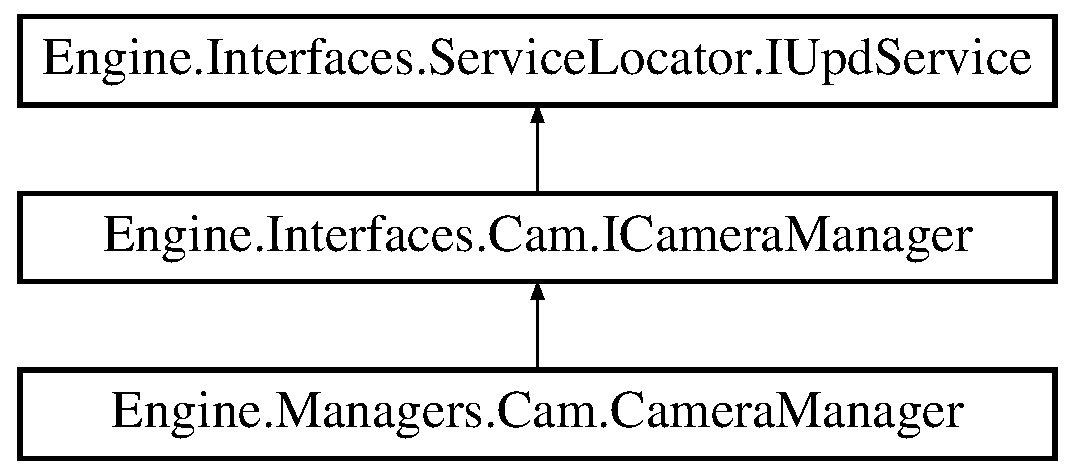
\includegraphics[height=3.000000cm]{d5/d0f/a00494}
\end{center}
\end{figure}
\subsection*{Public Member Functions}
\begin{DoxyCompactItemize}
\item 
void \hyperlink{a00494_a6244a0582982e64f49df0a6862768a21}{Initialize} ()
\begin{DoxyCompactList}\small\item\em M\+E\+T\+H\+OD\+: Creates a new camera \end{DoxyCompactList}\item 
\hyperlink{a00490}{Camera} \hyperlink{a00494_a949b09e5c57971945c3ccb638f73765d}{get\+Cam} ()
\begin{DoxyCompactList}\small\item\em M\+E\+T\+H\+OD\+: Returns the current \hyperlink{a00490}{Camera} \end{DoxyCompactList}\item 
void \hyperlink{a00494_a43e367859b47354445da2a304eff7ec4}{Update} (Game\+Time game\+Time)
\begin{DoxyCompactList}\small\item\em M\+E\+T\+H\+OD\+: Calls the update method of the \hyperlink{a00490}{Camera} that is being managed \end{DoxyCompactList}\item 
Vector2 \hyperlink{a00494_a538af3b5745f1f51e3da217d5c971791}{get\+World\+Position} (Vector2 Position)
\begin{DoxyCompactList}\small\item\em M\+E\+T\+H\+OD\+: returns the current world position in relation to the Vector2 provided \end{DoxyCompactList}\end{DoxyCompactItemize}


\subsection{Detailed Description}
C\+L\+A\+SS\+: A Manager for the camera, this is responsible for the creation of a \hyperlink{a00490}{Camera} object and updating it in relation to the world position 



\subsection{Member Function Documentation}
\mbox{\Hypertarget{a00494_a949b09e5c57971945c3ccb638f73765d}\label{a00494_a949b09e5c57971945c3ccb638f73765d}} 
\index{Engine\+::\+Managers\+::\+Cam\+::\+Camera\+Manager@{Engine\+::\+Managers\+::\+Cam\+::\+Camera\+Manager}!get\+Cam@{get\+Cam}}
\index{get\+Cam@{get\+Cam}!Engine\+::\+Managers\+::\+Cam\+::\+Camera\+Manager@{Engine\+::\+Managers\+::\+Cam\+::\+Camera\+Manager}}
\subsubsection{\texorpdfstring{get\+Cam()}{getCam()}}
{\footnotesize\ttfamily \hyperlink{a00490}{Camera} Engine.\+Managers.\+Cam.\+Camera\+Manager.\+get\+Cam (\begin{DoxyParamCaption}{ }\end{DoxyParamCaption})\hspace{0.3cm}{\ttfamily [inline]}}



M\+E\+T\+H\+OD\+: Returns the current \hyperlink{a00490}{Camera} 

\begin{DoxyReturn}{Returns}
The current \hyperlink{a00490}{Camera}
\end{DoxyReturn}


Implements \hyperlink{a00422_a91fc1dab51b36fd8955451ac00fd2819}{Engine.\+Interfaces.\+Cam.\+I\+Camera\+Manager}.

\mbox{\Hypertarget{a00494_a538af3b5745f1f51e3da217d5c971791}\label{a00494_a538af3b5745f1f51e3da217d5c971791}} 
\index{Engine\+::\+Managers\+::\+Cam\+::\+Camera\+Manager@{Engine\+::\+Managers\+::\+Cam\+::\+Camera\+Manager}!get\+World\+Position@{get\+World\+Position}}
\index{get\+World\+Position@{get\+World\+Position}!Engine\+::\+Managers\+::\+Cam\+::\+Camera\+Manager@{Engine\+::\+Managers\+::\+Cam\+::\+Camera\+Manager}}
\subsubsection{\texorpdfstring{get\+World\+Position()}{getWorldPosition()}}
{\footnotesize\ttfamily Vector2 Engine.\+Managers.\+Cam.\+Camera\+Manager.\+get\+World\+Position (\begin{DoxyParamCaption}\item[{Vector2}]{Position }\end{DoxyParamCaption})\hspace{0.3cm}{\ttfamily [inline]}}



M\+E\+T\+H\+OD\+: returns the current world position in relation to the Vector2 provided 


\begin{DoxyParams}{Parameters}
{\em Position} & The position to be compared to the world position\\
\hline
\end{DoxyParams}
\begin{DoxyReturn}{Returns}
The world position in relation to the Vector2 provided
\end{DoxyReturn}


Implements \hyperlink{a00422_a7d9fc1d792ddc3495bff23daac2a8d2a}{Engine.\+Interfaces.\+Cam.\+I\+Camera\+Manager}.

\mbox{\Hypertarget{a00494_a6244a0582982e64f49df0a6862768a21}\label{a00494_a6244a0582982e64f49df0a6862768a21}} 
\index{Engine\+::\+Managers\+::\+Cam\+::\+Camera\+Manager@{Engine\+::\+Managers\+::\+Cam\+::\+Camera\+Manager}!Initialize@{Initialize}}
\index{Initialize@{Initialize}!Engine\+::\+Managers\+::\+Cam\+::\+Camera\+Manager@{Engine\+::\+Managers\+::\+Cam\+::\+Camera\+Manager}}
\subsubsection{\texorpdfstring{Initialize()}{Initialize()}}
{\footnotesize\ttfamily void Engine.\+Managers.\+Cam.\+Camera\+Manager.\+Initialize (\begin{DoxyParamCaption}{ }\end{DoxyParamCaption})\hspace{0.3cm}{\ttfamily [inline]}}



M\+E\+T\+H\+OD\+: Creates a new camera 



Implements \hyperlink{a00422_a21e0ce6b0ada068546161ecf02559912}{Engine.\+Interfaces.\+Cam.\+I\+Camera\+Manager}.

\mbox{\Hypertarget{a00494_a43e367859b47354445da2a304eff7ec4}\label{a00494_a43e367859b47354445da2a304eff7ec4}} 
\index{Engine\+::\+Managers\+::\+Cam\+::\+Camera\+Manager@{Engine\+::\+Managers\+::\+Cam\+::\+Camera\+Manager}!Update@{Update}}
\index{Update@{Update}!Engine\+::\+Managers\+::\+Cam\+::\+Camera\+Manager@{Engine\+::\+Managers\+::\+Cam\+::\+Camera\+Manager}}
\subsubsection{\texorpdfstring{Update()}{Update()}}
{\footnotesize\ttfamily void Engine.\+Managers.\+Cam.\+Camera\+Manager.\+Update (\begin{DoxyParamCaption}\item[{Game\+Time}]{game\+Time }\end{DoxyParamCaption})\hspace{0.3cm}{\ttfamily [inline]}}



M\+E\+T\+H\+OD\+: Calls the update method of the \hyperlink{a00490}{Camera} that is being managed 


\begin{DoxyParams}{Parameters}
{\em game\+Time} & Monogame Game\+Time property\\
\hline
\end{DoxyParams}


Implements \hyperlink{a00422_a78a46559249e70181100daff38ef5d6a}{Engine.\+Interfaces.\+Cam.\+I\+Camera\+Manager}.



The documentation for this class was generated from the following file\+:\begin{DoxyCompactItemize}
\item 
\hyperlink{a00152}{Camera\+Manager.\+cs}\end{DoxyCompactItemize}

\hypertarget{a00350}{}\section{Engine.\+Events.\+Collision\+Event.\+Collision\+Event\+Args Class Reference}
\label{a00350}\index{Engine.\+Events.\+Collision\+Event.\+Collision\+Event\+Args@{Engine.\+Events.\+Collision\+Event.\+Collision\+Event\+Args}}
\subsection*{Properties}
\begin{DoxyCompactItemize}
\item 
\hyperlink{a00426}{I\+Collidable} \hyperlink{a00350_a15083f7089f32bacce7e1a41c1c04c4c}{A}\hspace{0.3cm}{\ttfamily  \mbox{[}get, set\mbox{]}}
\item 
\hyperlink{a00426}{I\+Collidable} \hyperlink{a00350_a2c08e8541c71e3c6c3d0574b7f4158c8}{B}\hspace{0.3cm}{\ttfamily  \mbox{[}get, set\mbox{]}}
\item 
Vector2 \hyperlink{a00350_a39df1ecc687f13296ef3a3dd09b007c6}{mtv\+Ret}\hspace{0.3cm}{\ttfamily  \mbox{[}get, set\mbox{]}}
\end{DoxyCompactItemize}


\subsection{Property Documentation}
\mbox{\Hypertarget{a00350_a15083f7089f32bacce7e1a41c1c04c4c}\label{a00350_a15083f7089f32bacce7e1a41c1c04c4c}} 
\index{Engine\+::\+Events\+::\+Collision\+Event\+::\+Collision\+Event\+Args@{Engine\+::\+Events\+::\+Collision\+Event\+::\+Collision\+Event\+Args}!A@{A}}
\index{A@{A}!Engine\+::\+Events\+::\+Collision\+Event\+::\+Collision\+Event\+Args@{Engine\+::\+Events\+::\+Collision\+Event\+::\+Collision\+Event\+Args}}
\subsubsection{\texorpdfstring{A}{A}}
{\footnotesize\ttfamily \hyperlink{a00426}{I\+Collidable} Engine.\+Events.\+Collision\+Event.\+Collision\+Event\+Args.\+A\hspace{0.3cm}{\ttfamily [get]}, {\ttfamily [set]}}

\mbox{\Hypertarget{a00350_a2c08e8541c71e3c6c3d0574b7f4158c8}\label{a00350_a2c08e8541c71e3c6c3d0574b7f4158c8}} 
\index{Engine\+::\+Events\+::\+Collision\+Event\+::\+Collision\+Event\+Args@{Engine\+::\+Events\+::\+Collision\+Event\+::\+Collision\+Event\+Args}!B@{B}}
\index{B@{B}!Engine\+::\+Events\+::\+Collision\+Event\+::\+Collision\+Event\+Args@{Engine\+::\+Events\+::\+Collision\+Event\+::\+Collision\+Event\+Args}}
\subsubsection{\texorpdfstring{B}{B}}
{\footnotesize\ttfamily \hyperlink{a00426}{I\+Collidable} Engine.\+Events.\+Collision\+Event.\+Collision\+Event\+Args.\+B\hspace{0.3cm}{\ttfamily [get]}, {\ttfamily [set]}}

\mbox{\Hypertarget{a00350_a39df1ecc687f13296ef3a3dd09b007c6}\label{a00350_a39df1ecc687f13296ef3a3dd09b007c6}} 
\index{Engine\+::\+Events\+::\+Collision\+Event\+::\+Collision\+Event\+Args@{Engine\+::\+Events\+::\+Collision\+Event\+::\+Collision\+Event\+Args}!mtv\+Ret@{mtv\+Ret}}
\index{mtv\+Ret@{mtv\+Ret}!Engine\+::\+Events\+::\+Collision\+Event\+::\+Collision\+Event\+Args@{Engine\+::\+Events\+::\+Collision\+Event\+::\+Collision\+Event\+Args}}
\subsubsection{\texorpdfstring{mtv\+Ret}{mtvRet}}
{\footnotesize\ttfamily Vector2 Engine.\+Events.\+Collision\+Event.\+Collision\+Event\+Args.\+mtv\+Ret\hspace{0.3cm}{\ttfamily [get]}, {\ttfamily [set]}}



The documentation for this class was generated from the following file\+:\begin{DoxyCompactItemize}
\item 
\hyperlink{a00044}{Collision\+Event\+Args.\+cs}\end{DoxyCompactItemize}

\hypertarget{a00354}{}\section{Engine.\+Events.\+Collision\+Event.\+Collision\+Handler Class Reference}
\label{a00354}\index{Engine.\+Events.\+Collision\+Event.\+Collision\+Handler@{Engine.\+Events.\+Collision\+Event.\+Collision\+Handler}}
\subsection*{Public Member Functions}
\begin{DoxyCompactItemize}
\item 
delegate void \hyperlink{a00354_a2e6e57bf1eda856c51464dfd560c2151}{Collision\+Event\+Handler} (object sender, \hyperlink{a00350}{Collision\+Event\+Args} e)
\item 
void \hyperlink{a00354_abfa92089bdf2aaa93c332e32737d4531}{Update} ()
\item 
void \hyperlink{a00354_a99ec43d39ea173a2a5897691228bea98}{Collision} ()
\end{DoxyCompactItemize}
\subsection*{Properties}
\begin{DoxyCompactItemize}
\item 
static \hyperlink{a00354}{Collision\+Handler} \hyperlink{a00354_a9106bf24803f79138e8cf42162c7ec82}{Instance}\hspace{0.3cm}{\ttfamily  \mbox{[}get\mbox{]}}
\end{DoxyCompactItemize}
\subsection*{Events}
\begin{DoxyCompactItemize}
\item 
\hyperlink{a00354_a2e6e57bf1eda856c51464dfd560c2151}{Collision\+Event\+Handler} \hyperlink{a00354_aa1c9eb18623260839928ff18e8aa6e5b}{On\+Collision}
\end{DoxyCompactItemize}


\subsection{Member Function Documentation}
\mbox{\Hypertarget{a00354_a99ec43d39ea173a2a5897691228bea98}\label{a00354_a99ec43d39ea173a2a5897691228bea98}} 
\index{Engine\+::\+Events\+::\+Collision\+Event\+::\+Collision\+Handler@{Engine\+::\+Events\+::\+Collision\+Event\+::\+Collision\+Handler}!Collision@{Collision}}
\index{Collision@{Collision}!Engine\+::\+Events\+::\+Collision\+Event\+::\+Collision\+Handler@{Engine\+::\+Events\+::\+Collision\+Event\+::\+Collision\+Handler}}
\subsubsection{\texorpdfstring{Collision()}{Collision()}}
{\footnotesize\ttfamily void Engine.\+Events.\+Collision\+Event.\+Collision\+Handler.\+Collision (\begin{DoxyParamCaption}{ }\end{DoxyParamCaption})\hspace{0.3cm}{\ttfamily [inline]}}

\mbox{\Hypertarget{a00354_a2e6e57bf1eda856c51464dfd560c2151}\label{a00354_a2e6e57bf1eda856c51464dfd560c2151}} 
\index{Engine\+::\+Events\+::\+Collision\+Event\+::\+Collision\+Handler@{Engine\+::\+Events\+::\+Collision\+Event\+::\+Collision\+Handler}!Collision\+Event\+Handler@{Collision\+Event\+Handler}}
\index{Collision\+Event\+Handler@{Collision\+Event\+Handler}!Engine\+::\+Events\+::\+Collision\+Event\+::\+Collision\+Handler@{Engine\+::\+Events\+::\+Collision\+Event\+::\+Collision\+Handler}}
\subsubsection{\texorpdfstring{Collision\+Event\+Handler()}{CollisionEventHandler()}}
{\footnotesize\ttfamily delegate void Engine.\+Events.\+Collision\+Event.\+Collision\+Handler.\+Collision\+Event\+Handler (\begin{DoxyParamCaption}\item[{object}]{sender,  }\item[{\hyperlink{a00350}{Collision\+Event\+Args}}]{e }\end{DoxyParamCaption})}

\mbox{\Hypertarget{a00354_abfa92089bdf2aaa93c332e32737d4531}\label{a00354_abfa92089bdf2aaa93c332e32737d4531}} 
\index{Engine\+::\+Events\+::\+Collision\+Event\+::\+Collision\+Handler@{Engine\+::\+Events\+::\+Collision\+Event\+::\+Collision\+Handler}!Update@{Update}}
\index{Update@{Update}!Engine\+::\+Events\+::\+Collision\+Event\+::\+Collision\+Handler@{Engine\+::\+Events\+::\+Collision\+Event\+::\+Collision\+Handler}}
\subsubsection{\texorpdfstring{Update()}{Update()}}
{\footnotesize\ttfamily void Engine.\+Events.\+Collision\+Event.\+Collision\+Handler.\+Update (\begin{DoxyParamCaption}{ }\end{DoxyParamCaption})\hspace{0.3cm}{\ttfamily [inline]}}



\subsection{Property Documentation}
\mbox{\Hypertarget{a00354_a9106bf24803f79138e8cf42162c7ec82}\label{a00354_a9106bf24803f79138e8cf42162c7ec82}} 
\index{Engine\+::\+Events\+::\+Collision\+Event\+::\+Collision\+Handler@{Engine\+::\+Events\+::\+Collision\+Event\+::\+Collision\+Handler}!Instance@{Instance}}
\index{Instance@{Instance}!Engine\+::\+Events\+::\+Collision\+Event\+::\+Collision\+Handler@{Engine\+::\+Events\+::\+Collision\+Event\+::\+Collision\+Handler}}
\subsubsection{\texorpdfstring{Instance}{Instance}}
{\footnotesize\ttfamily \hyperlink{a00354}{Collision\+Handler} Engine.\+Events.\+Collision\+Event.\+Collision\+Handler.\+Instance\hspace{0.3cm}{\ttfamily [static]}, {\ttfamily [get]}}



\subsection{Event Documentation}
\mbox{\Hypertarget{a00354_aa1c9eb18623260839928ff18e8aa6e5b}\label{a00354_aa1c9eb18623260839928ff18e8aa6e5b}} 
\index{Engine\+::\+Events\+::\+Collision\+Event\+::\+Collision\+Handler@{Engine\+::\+Events\+::\+Collision\+Event\+::\+Collision\+Handler}!On\+Collision@{On\+Collision}}
\index{On\+Collision@{On\+Collision}!Engine\+::\+Events\+::\+Collision\+Event\+::\+Collision\+Handler@{Engine\+::\+Events\+::\+Collision\+Event\+::\+Collision\+Handler}}
\subsubsection{\texorpdfstring{On\+Collision}{OnCollision}}
{\footnotesize\ttfamily \hyperlink{a00354_a2e6e57bf1eda856c51464dfd560c2151}{Collision\+Event\+Handler} Engine.\+Events.\+Collision\+Event.\+Collision\+Handler.\+On\+Collision}



The documentation for this class was generated from the following file\+:\begin{DoxyCompactItemize}
\item 
\hyperlink{a00047}{Collision\+Handler.\+cs}\end{DoxyCompactItemize}

\hypertarget{a00314}{}\section{Engine.\+Entities.\+Entity Class Reference}
\label{a00314}\index{Engine.\+Entities.\+Entity@{Engine.\+Entities.\+Entity}}


A\+B\+S\+T\+R\+A\+CT C\+L\+A\+SS\+: The Base entity class. All entities extend this class. It contains the basic setup and properties of each entity.  


Inheritance diagram for Engine.\+Entities.\+Entity\+:\begin{figure}[H]
\begin{center}
\leavevmode
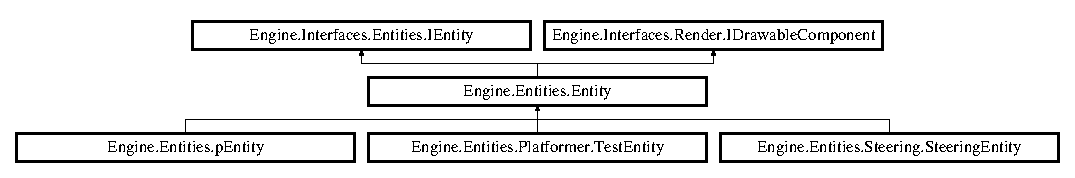
\includegraphics[height=1.944444cm]{d0/d39/a00314}
\end{center}
\end{figure}
\subsection*{Public Member Functions}
\begin{DoxyCompactItemize}
\item 
\hyperlink{a00314_a5a3cc22ef87965c27e86f8b0867550cf}{Entity} ()
\begin{DoxyCompactList}\small\item\em C\+O\+N\+S\+T\+R\+U\+C\+T\+OR\+: Sets the basic properties for the entity. \end{DoxyCompactList}\item 
virtual void \hyperlink{a00314_aa1425aeeac379c5141e7560b84850b3d}{Initialize} (Vector2 Pos)
\begin{DoxyCompactList}\small\item\em M\+E\+T\+H\+OD\+: Initialises the basic properties of this entity, such as the mind \end{DoxyCompactList}\item 
void \hyperlink{a00314_a5c795930028c5672b54f95369b25019f}{Draw} (Sprite\+Batch sprite\+Batch)
\begin{DoxyCompactList}\small\item\em M\+E\+T\+H\+OD\+: Draw the entitity \end{DoxyCompactList}\end{DoxyCompactItemize}
\subsection*{Protected Attributes}
\begin{DoxyCompactItemize}
\item 
\hyperlink{a00446}{I\+Mind} \hyperlink{a00314_a8ba8155440726f55d5e087eeecf0d12f}{mind}
\begin{DoxyCompactList}\small\item\em D\+E\+C\+L\+A\+RE\+: The mind that controls the entity. \end{DoxyCompactList}\end{DoxyCompactItemize}
\subsection*{Properties}
\begin{DoxyCompactItemize}
\item 
Vector2 \hyperlink{a00314_a1821405e931e09c3a3b264d6b9fd9011}{Velocity}\hspace{0.3cm}{\ttfamily  \mbox{[}get\mbox{]}}
\begin{DoxyCompactList}\small\item\em G\+ET\+: The velocity of the entity. \end{DoxyCompactList}\item 
int \hyperlink{a00314_a2f119510debb21928206de4a3c47fc00}{Unique\+ID}\hspace{0.3cm}{\ttfamily  \mbox{[}get, protected set\mbox{]}}
\begin{DoxyCompactList}\small\item\em G\+ET\+: S\+ET\+: The unique ID for an \hyperlink{a00314}{Entity}. \end{DoxyCompactList}\item 
bool \hyperlink{a00314_a519bb560bd5dda64938b48d28c368508}{is\+Visible}\hspace{0.3cm}{\ttfamily  \mbox{[}get, set\mbox{]}}
\begin{DoxyCompactList}\small\item\em G\+ET\+: S\+ET\+: whether the entity needs to be drawn or not. \end{DoxyCompactList}\item 
string \hyperlink{a00314_a2f3828a9c39ae5b5643ca1debd254384}{Name}\hspace{0.3cm}{\ttfamily  \mbox{[}get, set\mbox{]}}
\item 
Vector2 \hyperlink{a00314_a5324a089780eefc8749e5794a47a53be}{Position}\hspace{0.3cm}{\ttfamily  \mbox{[}get, set\mbox{]}}
\begin{DoxyCompactList}\small\item\em G\+ET\+: S\+ET\+: The position of the entity. \end{DoxyCompactList}\item 
Texture2D \hyperlink{a00314_a2ab6afa4c8cc6f8dede6c2a18f483970}{Texture}\hspace{0.3cm}{\ttfamily  \mbox{[}get, set\mbox{]}}
\begin{DoxyCompactList}\small\item\em G\+ET\+: S\+ET\+: The texture of the entity. \end{DoxyCompactList}\item 
Rectangle \hyperlink{a00314_a364d5fcdaee8aa472c0b8fb35830abd8}{Bounds}\hspace{0.3cm}{\ttfamily  \mbox{[}get\mbox{]}}
\begin{DoxyCompactList}\small\item\em G\+ET\+: S\+ET\+: The Axis aligned bounds of the entity. \end{DoxyCompactList}\item 
bool \hyperlink{a00314_ae1da9f3aba0ba07c837ac2ccda590139}{is\+Collidable}\hspace{0.3cm}{\ttfamily  \mbox{[}get, set\mbox{]}}
\begin{DoxyCompactList}\small\item\em G\+ET\+: S\+ET\+: A bool to check whether the entity needs to be included in collision calculations \end{DoxyCompactList}\end{DoxyCompactItemize}


\subsection{Detailed Description}
A\+B\+S\+T\+R\+A\+CT C\+L\+A\+SS\+: The Base entity class. All entities extend this class. It contains the basic setup and properties of each entity. 



\subsection{Constructor \& Destructor Documentation}
\mbox{\Hypertarget{a00314_a5a3cc22ef87965c27e86f8b0867550cf}\label{a00314_a5a3cc22ef87965c27e86f8b0867550cf}} 
\index{Engine\+::\+Entities\+::\+Entity@{Engine\+::\+Entities\+::\+Entity}!Entity@{Entity}}
\index{Entity@{Entity}!Engine\+::\+Entities\+::\+Entity@{Engine\+::\+Entities\+::\+Entity}}
\subsubsection{\texorpdfstring{Entity()}{Entity()}}
{\footnotesize\ttfamily Engine.\+Entities.\+Entity.\+Entity (\begin{DoxyParamCaption}{ }\end{DoxyParamCaption})\hspace{0.3cm}{\ttfamily [inline]}}



C\+O\+N\+S\+T\+R\+U\+C\+T\+OR\+: Sets the basic properties for the entity. 

S\+ET\+: The unique ID of the entity.

I\+N\+C\+R\+E\+M\+E\+NT\+: The ID count for the next entity

S\+ET\+: The name of the entity 

\subsection{Member Function Documentation}
\mbox{\Hypertarget{a00314_a5c795930028c5672b54f95369b25019f}\label{a00314_a5c795930028c5672b54f95369b25019f}} 
\index{Engine\+::\+Entities\+::\+Entity@{Engine\+::\+Entities\+::\+Entity}!Draw@{Draw}}
\index{Draw@{Draw}!Engine\+::\+Entities\+::\+Entity@{Engine\+::\+Entities\+::\+Entity}}
\subsubsection{\texorpdfstring{Draw()}{Draw()}}
{\footnotesize\ttfamily void Engine.\+Entities.\+Entity.\+Draw (\begin{DoxyParamCaption}\item[{Sprite\+Batch}]{sprite\+Batch }\end{DoxyParamCaption})\hspace{0.3cm}{\ttfamily [inline]}}



M\+E\+T\+H\+OD\+: Draw the entitity 


\begin{DoxyParams}{Parameters}
{\em sprite\+Batch} & \\
\hline
\end{DoxyParams}
C\+A\+LL\+: The spritebatch draw method. 

Implements \hyperlink{a00438_a845918af6647460d2c47a3853a30f95f}{Engine.\+Interfaces.\+Entities.\+I\+Entity}.

\mbox{\Hypertarget{a00314_aa1425aeeac379c5141e7560b84850b3d}\label{a00314_aa1425aeeac379c5141e7560b84850b3d}} 
\index{Engine\+::\+Entities\+::\+Entity@{Engine\+::\+Entities\+::\+Entity}!Initialize@{Initialize}}
\index{Initialize@{Initialize}!Engine\+::\+Entities\+::\+Entity@{Engine\+::\+Entities\+::\+Entity}}
\subsubsection{\texorpdfstring{Initialize()}{Initialize()}}
{\footnotesize\ttfamily virtual void Engine.\+Entities.\+Entity.\+Initialize (\begin{DoxyParamCaption}\item[{Vector2}]{Pos }\end{DoxyParamCaption})\hspace{0.3cm}{\ttfamily [inline]}, {\ttfamily [virtual]}}



M\+E\+T\+H\+OD\+: Initialises the basic properties of this entity, such as the mind 


\begin{DoxyParams}{Parameters}
{\em Pos} & \\
\hline
\end{DoxyParams}
IF\+: The mind is not null, T\+H\+EN initialise the mind. 

Implements \hyperlink{a00438_a0c80525509aaeaa0d78eef908f7f7553}{Engine.\+Interfaces.\+Entities.\+I\+Entity}.



Reimplemented in \hyperlink{a00322_aad953baa984c0f958d3e96efbfc3bca9}{Engine.\+Entities.\+p\+Entity}, \hyperlink{a00330_ad4122c4f38d98746a67532d0a6836da5}{Engine.\+Entities.\+Platformer.\+Test\+Entity}, and \hyperlink{a00342_a7b1e3df5320c999d2cf1cc3b97994401}{Engine.\+Entities.\+Steering.\+Steering\+Entity}.



\subsection{Field Documentation}
\mbox{\Hypertarget{a00314_a8ba8155440726f55d5e087eeecf0d12f}\label{a00314_a8ba8155440726f55d5e087eeecf0d12f}} 
\index{Engine\+::\+Entities\+::\+Entity@{Engine\+::\+Entities\+::\+Entity}!mind@{mind}}
\index{mind@{mind}!Engine\+::\+Entities\+::\+Entity@{Engine\+::\+Entities\+::\+Entity}}
\subsubsection{\texorpdfstring{mind}{mind}}
{\footnotesize\ttfamily \hyperlink{a00446}{I\+Mind} Engine.\+Entities.\+Entity.\+mind\hspace{0.3cm}{\ttfamily [protected]}}



D\+E\+C\+L\+A\+RE\+: The mind that controls the entity. 



\subsection{Property Documentation}
\mbox{\Hypertarget{a00314_a364d5fcdaee8aa472c0b8fb35830abd8}\label{a00314_a364d5fcdaee8aa472c0b8fb35830abd8}} 
\index{Engine\+::\+Entities\+::\+Entity@{Engine\+::\+Entities\+::\+Entity}!Bounds@{Bounds}}
\index{Bounds@{Bounds}!Engine\+::\+Entities\+::\+Entity@{Engine\+::\+Entities\+::\+Entity}}
\subsubsection{\texorpdfstring{Bounds}{Bounds}}
{\footnotesize\ttfamily Rectangle Engine.\+Entities.\+Entity.\+Bounds\hspace{0.3cm}{\ttfamily [get]}}



G\+ET\+: S\+ET\+: The Axis aligned bounds of the entity. 

\mbox{\Hypertarget{a00314_ae1da9f3aba0ba07c837ac2ccda590139}\label{a00314_ae1da9f3aba0ba07c837ac2ccda590139}} 
\index{Engine\+::\+Entities\+::\+Entity@{Engine\+::\+Entities\+::\+Entity}!is\+Collidable@{is\+Collidable}}
\index{is\+Collidable@{is\+Collidable}!Engine\+::\+Entities\+::\+Entity@{Engine\+::\+Entities\+::\+Entity}}
\subsubsection{\texorpdfstring{is\+Collidable}{isCollidable}}
{\footnotesize\ttfamily bool Engine.\+Entities.\+Entity.\+is\+Collidable\hspace{0.3cm}{\ttfamily [get]}, {\ttfamily [set]}}



G\+ET\+: S\+ET\+: A bool to check whether the entity needs to be included in collision calculations 

\mbox{\Hypertarget{a00314_a519bb560bd5dda64938b48d28c368508}\label{a00314_a519bb560bd5dda64938b48d28c368508}} 
\index{Engine\+::\+Entities\+::\+Entity@{Engine\+::\+Entities\+::\+Entity}!is\+Visible@{is\+Visible}}
\index{is\+Visible@{is\+Visible}!Engine\+::\+Entities\+::\+Entity@{Engine\+::\+Entities\+::\+Entity}}
\subsubsection{\texorpdfstring{is\+Visible}{isVisible}}
{\footnotesize\ttfamily bool Engine.\+Entities.\+Entity.\+is\+Visible\hspace{0.3cm}{\ttfamily [get]}, {\ttfamily [set]}}



G\+ET\+: S\+ET\+: whether the entity needs to be drawn or not. 

\mbox{\Hypertarget{a00314_a2f3828a9c39ae5b5643ca1debd254384}\label{a00314_a2f3828a9c39ae5b5643ca1debd254384}} 
\index{Engine\+::\+Entities\+::\+Entity@{Engine\+::\+Entities\+::\+Entity}!Name@{Name}}
\index{Name@{Name}!Engine\+::\+Entities\+::\+Entity@{Engine\+::\+Entities\+::\+Entity}}
\subsubsection{\texorpdfstring{Name}{Name}}
{\footnotesize\ttfamily string Engine.\+Entities.\+Entity.\+Name\hspace{0.3cm}{\ttfamily [get]}, {\ttfamily [set]}}

\mbox{\Hypertarget{a00314_a5324a089780eefc8749e5794a47a53be}\label{a00314_a5324a089780eefc8749e5794a47a53be}} 
\index{Engine\+::\+Entities\+::\+Entity@{Engine\+::\+Entities\+::\+Entity}!Position@{Position}}
\index{Position@{Position}!Engine\+::\+Entities\+::\+Entity@{Engine\+::\+Entities\+::\+Entity}}
\subsubsection{\texorpdfstring{Position}{Position}}
{\footnotesize\ttfamily Vector2 Engine.\+Entities.\+Entity.\+Position\hspace{0.3cm}{\ttfamily [get]}, {\ttfamily [set]}}



G\+ET\+: S\+ET\+: The position of the entity. 

\mbox{\Hypertarget{a00314_a2ab6afa4c8cc6f8dede6c2a18f483970}\label{a00314_a2ab6afa4c8cc6f8dede6c2a18f483970}} 
\index{Engine\+::\+Entities\+::\+Entity@{Engine\+::\+Entities\+::\+Entity}!Texture@{Texture}}
\index{Texture@{Texture}!Engine\+::\+Entities\+::\+Entity@{Engine\+::\+Entities\+::\+Entity}}
\subsubsection{\texorpdfstring{Texture}{Texture}}
{\footnotesize\ttfamily Texture2D Engine.\+Entities.\+Entity.\+Texture\hspace{0.3cm}{\ttfamily [get]}, {\ttfamily [set]}}



G\+ET\+: S\+ET\+: The texture of the entity. 

\mbox{\Hypertarget{a00314_a2f119510debb21928206de4a3c47fc00}\label{a00314_a2f119510debb21928206de4a3c47fc00}} 
\index{Engine\+::\+Entities\+::\+Entity@{Engine\+::\+Entities\+::\+Entity}!Unique\+ID@{Unique\+ID}}
\index{Unique\+ID@{Unique\+ID}!Engine\+::\+Entities\+::\+Entity@{Engine\+::\+Entities\+::\+Entity}}
\subsubsection{\texorpdfstring{Unique\+ID}{UniqueID}}
{\footnotesize\ttfamily int Engine.\+Entities.\+Entity.\+Unique\+ID\hspace{0.3cm}{\ttfamily [get]}, {\ttfamily [protected set]}}



G\+ET\+: S\+ET\+: The unique ID for an \hyperlink{a00314}{Entity}. 

\mbox{\Hypertarget{a00314_a1821405e931e09c3a3b264d6b9fd9011}\label{a00314_a1821405e931e09c3a3b264d6b9fd9011}} 
\index{Engine\+::\+Entities\+::\+Entity@{Engine\+::\+Entities\+::\+Entity}!Velocity@{Velocity}}
\index{Velocity@{Velocity}!Engine\+::\+Entities\+::\+Entity@{Engine\+::\+Entities\+::\+Entity}}
\subsubsection{\texorpdfstring{Velocity}{Velocity}}
{\footnotesize\ttfamily Vector2 Engine.\+Entities.\+Entity.\+Velocity\hspace{0.3cm}{\ttfamily [get]}}



G\+ET\+: The velocity of the entity. 



The documentation for this class was generated from the following file\+:\begin{DoxyCompactItemize}
\item 
\hyperlink{a00017}{Entity.\+cs}\end{DoxyCompactItemize}

\hypertarget{a00518}{}\section{Engine.\+Managers.\+Entities.\+Entity\+Manager Class Reference}
\label{a00518}\index{Engine.\+Managers.\+Entities.\+Entity\+Manager@{Engine.\+Managers.\+Entities.\+Entity\+Manager}}


C\+L\+A\+SS\+: Entity Manager is responsible for the creation and storage of all entities in the game scene. It is able to return a list, a specific entity, or create and remove entities from the scene  


Inheritance diagram for Engine.\+Managers.\+Entities.\+Entity\+Manager\+:\begin{figure}[H]
\begin{center}
\leavevmode
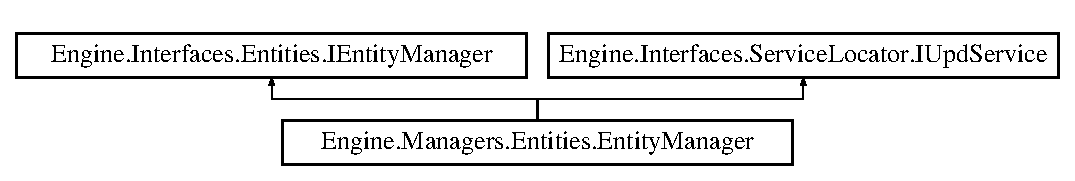
\includegraphics[height=1.978799cm]{d5/dee/a00518}
\end{center}
\end{figure}
\subsection*{Public Member Functions}
\begin{DoxyCompactItemize}
\item 
\hyperlink{a00518_a0fd18e00f80a32046831041574e8a6a8}{Entity\+Manager} ()
\begin{DoxyCompactList}\small\item\em C\+O\+N\+S\+T\+R\+U\+C\+T\+OR \end{DoxyCompactList}\item 
List$<$ \hyperlink{a00438}{I\+Entity} $>$ \hyperlink{a00518_a704e3c8fb916a8bb668ffd30654b4e18}{get\+List} ()
\begin{DoxyCompactList}\small\item\em M\+E\+T\+H\+OD\+: returns a list of entities \end{DoxyCompactList}\item 
List$<$ \hyperlink{a00438}{I\+Entity} $>$ \hyperlink{a00518_a13ec76267682ed1ce3ace63c561ec6c5}{get\+Cam\+List} ()
\begin{DoxyCompactList}\small\item\em M\+E\+T\+H\+OD\+: Returns a list of entities requiring a camera \end{DoxyCompactList}\item 
void \hyperlink{a00518_a33cf4a636f70486e8a13c52bb4395cd6}{add\+Entity} (\hyperlink{a00438}{I\+Entity} e)
\begin{DoxyCompactList}\small\item\em M\+E\+T\+H\+OD\+: Add an entity to the list of entities \end{DoxyCompactList}\item 
void \hyperlink{a00518_a5b84d299c11d42065f55048dd14fdd4c}{add\+Cam\+Entity} (\hyperlink{a00438}{I\+Entity} e)
\begin{DoxyCompactList}\small\item\em M\+E\+T\+H\+OD\+: Add an entity requiring a camera to the list of entities \end{DoxyCompactList}\item 
\hyperlink{a00438}{I\+Entity} \hyperlink{a00518_a228280a4515648318fb5528936249a8b}{create\+Entity$<$ T $>$} (Vector2 Position)
\begin{DoxyCompactList}\small\item\em M\+E\+T\+H\+OD\+: Create a new entity and add it to the entity List \end{DoxyCompactList}\item 
\hyperlink{a00438}{I\+Entity} \hyperlink{a00518_a89ca1b1834aff0dc1d2c6ec95dcd0793}{create\+Entity\+Cam\+Drawable$<$ T $>$} (Vector2 Position)
\begin{DoxyCompactList}\small\item\em M\+E\+T\+H\+OD\+: Create a new Camera entity and add it to the camera entity list \end{DoxyCompactList}\item 
\hyperlink{a00438}{I\+Entity} \hyperlink{a00518_a787212a79eb20bd2c695783b5f802347}{create\+Entity\+Drawable$<$ T $>$} (Vector2 Position)
\begin{DoxyCompactList}\small\item\em M\+E\+T\+H\+OD\+: Create a new Drawable entity and add it to the Camera list \end{DoxyCompactList}\item 
void \hyperlink{a00518_a960c2ec6b45bbbd4f0030b04f90dc407}{temp\+Cam\+Clear} ()
\begin{DoxyCompactList}\small\item\em M\+E\+T\+H\+OD\+: Clear all camera entities \end{DoxyCompactList}\item 
void \hyperlink{a00518_abeffd88412f79249f333944b45486dff}{get\+Entity} (string name)
\begin{DoxyCompactList}\small\item\em M\+E\+T\+H\+OD\+: Get an entity by it\textquotesingle{}s name \end{DoxyCompactList}\item 
\hyperlink{a00438}{I\+Entity} \hyperlink{a00518_ab3ff805a060af38748444e520995d8fa}{get\+Cam\+Entity} (string name)
\begin{DoxyCompactList}\small\item\em M\+E\+T\+H\+OD\+: Get a Camera I\+Entity by it;s name \end{DoxyCompactList}\item 
void \hyperlink{a00518_a4eff29b463061f602be758bd3d36ef25}{clear\+List} ()
\begin{DoxyCompactList}\small\item\em M\+E\+T\+H\+OD\+: Clear the list of all I\+Entities \end{DoxyCompactList}\item 
void \hyperlink{a00518_a1d9ffc3b80cc8633265fe1f7e51c6122}{remove\+Entity} (int entity\+ID)
\begin{DoxyCompactList}\small\item\em M\+E\+T\+H\+OD\+: Remove a specific I\+Entity from the manager and list of Ientities \end{DoxyCompactList}\item 
void \hyperlink{a00518_a5f4c775a02bbb9057577780643a7b068}{remove\+Cam\+Entity} (int entity\+ID)
\begin{DoxyCompactList}\small\item\em M\+E\+T\+H\+OD\+: Remove a specific Camera entity by it;s ID \end{DoxyCompactList}\item 
void \hyperlink{a00518_a386e96f9edb12689118de624c559de0f}{Update} (Game\+Time game\+Time)
\begin{DoxyCompactList}\small\item\em M\+E\+T\+H\+OD\+: The Update loop that is called every frame \end{DoxyCompactList}\end{DoxyCompactItemize}


\subsection{Detailed Description}
C\+L\+A\+SS\+: Entity Manager is responsible for the creation and storage of all entities in the game scene. It is able to return a list, a specific entity, or create and remove entities from the scene 



\subsection{Constructor \& Destructor Documentation}
\mbox{\Hypertarget{a00518_a0fd18e00f80a32046831041574e8a6a8}\label{a00518_a0fd18e00f80a32046831041574e8a6a8}} 
\index{Engine\+::\+Managers\+::\+Entities\+::\+Entity\+Manager@{Engine\+::\+Managers\+::\+Entities\+::\+Entity\+Manager}!Entity\+Manager@{Entity\+Manager}}
\index{Entity\+Manager@{Entity\+Manager}!Engine\+::\+Managers\+::\+Entities\+::\+Entity\+Manager@{Engine\+::\+Managers\+::\+Entities\+::\+Entity\+Manager}}
\subsubsection{\texorpdfstring{Entity\+Manager()}{EntityManager()}}
{\footnotesize\ttfamily Engine.\+Managers.\+Entities.\+Entity\+Manager.\+Entity\+Manager (\begin{DoxyParamCaption}{ }\end{DoxyParamCaption})\hspace{0.3cm}{\ttfamily [inline]}}



C\+O\+N\+S\+T\+R\+U\+C\+T\+OR 



\subsection{Member Function Documentation}
\mbox{\Hypertarget{a00518_a5b84d299c11d42065f55048dd14fdd4c}\label{a00518_a5b84d299c11d42065f55048dd14fdd4c}} 
\index{Engine\+::\+Managers\+::\+Entities\+::\+Entity\+Manager@{Engine\+::\+Managers\+::\+Entities\+::\+Entity\+Manager}!add\+Cam\+Entity@{add\+Cam\+Entity}}
\index{add\+Cam\+Entity@{add\+Cam\+Entity}!Engine\+::\+Managers\+::\+Entities\+::\+Entity\+Manager@{Engine\+::\+Managers\+::\+Entities\+::\+Entity\+Manager}}
\subsubsection{\texorpdfstring{add\+Cam\+Entity()}{addCamEntity()}}
{\footnotesize\ttfamily void Engine.\+Managers.\+Entities.\+Entity\+Manager.\+add\+Cam\+Entity (\begin{DoxyParamCaption}\item[{\hyperlink{a00438}{I\+Entity}}]{e }\end{DoxyParamCaption})\hspace{0.3cm}{\ttfamily [inline]}}



M\+E\+T\+H\+OD\+: Add an entity requiring a camera to the list of entities 


\begin{DoxyParams}{Parameters}
{\em e} & The entity to be added to the camera entity list\\
\hline
\end{DoxyParams}


Implements \hyperlink{a00442_a37055c1d97dd8da61a53a2b0683df54d}{Engine.\+Interfaces.\+Entities.\+I\+Entity\+Manager}.

\mbox{\Hypertarget{a00518_a33cf4a636f70486e8a13c52bb4395cd6}\label{a00518_a33cf4a636f70486e8a13c52bb4395cd6}} 
\index{Engine\+::\+Managers\+::\+Entities\+::\+Entity\+Manager@{Engine\+::\+Managers\+::\+Entities\+::\+Entity\+Manager}!add\+Entity@{add\+Entity}}
\index{add\+Entity@{add\+Entity}!Engine\+::\+Managers\+::\+Entities\+::\+Entity\+Manager@{Engine\+::\+Managers\+::\+Entities\+::\+Entity\+Manager}}
\subsubsection{\texorpdfstring{add\+Entity()}{addEntity()}}
{\footnotesize\ttfamily void Engine.\+Managers.\+Entities.\+Entity\+Manager.\+add\+Entity (\begin{DoxyParamCaption}\item[{\hyperlink{a00438}{I\+Entity}}]{e }\end{DoxyParamCaption})\hspace{0.3cm}{\ttfamily [inline]}}



M\+E\+T\+H\+OD\+: Add an entity to the list of entities 


\begin{DoxyParams}{Parameters}
{\em e} & The entity to be added to the list\\
\hline
\end{DoxyParams}


Implements \hyperlink{a00442_af229fa3936a8483383bb7ddd5b4184b0}{Engine.\+Interfaces.\+Entities.\+I\+Entity\+Manager}.

\mbox{\Hypertarget{a00518_a4eff29b463061f602be758bd3d36ef25}\label{a00518_a4eff29b463061f602be758bd3d36ef25}} 
\index{Engine\+::\+Managers\+::\+Entities\+::\+Entity\+Manager@{Engine\+::\+Managers\+::\+Entities\+::\+Entity\+Manager}!clear\+List@{clear\+List}}
\index{clear\+List@{clear\+List}!Engine\+::\+Managers\+::\+Entities\+::\+Entity\+Manager@{Engine\+::\+Managers\+::\+Entities\+::\+Entity\+Manager}}
\subsubsection{\texorpdfstring{clear\+List()}{clearList()}}
{\footnotesize\ttfamily void Engine.\+Managers.\+Entities.\+Entity\+Manager.\+clear\+List (\begin{DoxyParamCaption}{ }\end{DoxyParamCaption})\hspace{0.3cm}{\ttfamily [inline]}}



M\+E\+T\+H\+OD\+: Clear the list of all I\+Entities 



Implements \hyperlink{a00442_acccc889cc99843899ce0652a9959e907}{Engine.\+Interfaces.\+Entities.\+I\+Entity\+Manager}.

\mbox{\Hypertarget{a00518_a228280a4515648318fb5528936249a8b}\label{a00518_a228280a4515648318fb5528936249a8b}} 
\index{Engine\+::\+Managers\+::\+Entities\+::\+Entity\+Manager@{Engine\+::\+Managers\+::\+Entities\+::\+Entity\+Manager}!create\+Entity$<$ T $>$@{create\+Entity$<$ T $>$}}
\index{create\+Entity$<$ T $>$@{create\+Entity$<$ T $>$}!Engine\+::\+Managers\+::\+Entities\+::\+Entity\+Manager@{Engine\+::\+Managers\+::\+Entities\+::\+Entity\+Manager}}
\subsubsection{\texorpdfstring{create\+Entity$<$ T $>$()}{createEntity< T >()}}
{\footnotesize\ttfamily \hyperlink{a00438}{I\+Entity} Engine.\+Managers.\+Entities.\+Entity\+Manager.\+create\+Entity$<$ T $>$ (\begin{DoxyParamCaption}\item[{Vector2}]{Position }\end{DoxyParamCaption})\hspace{0.3cm}{\ttfamily [inline]}}



M\+E\+T\+H\+OD\+: Create a new entity and add it to the entity List 


\begin{DoxyTemplParams}{Template Parameters}
{\em T} & The generic I\+Entity object to be created\\
\hline
\end{DoxyTemplParams}

\begin{DoxyParams}{Parameters}
{\em Position} & The position to create the object at\\
\hline
\end{DoxyParams}
\begin{DoxyReturn}{Returns}

\end{DoxyReturn}


Implements \hyperlink{a00442_a8f746b319d35a76cb4cdb1853f3069ed}{Engine.\+Interfaces.\+Entities.\+I\+Entity\+Manager}.

\begin{Desc}
\item[Type Constraints]\begin{description}
\item[{\em T} : {\em I\+Entity}]\item[{\em T} : {\em new()}]\end{description}
\end{Desc}
\mbox{\Hypertarget{a00518_a89ca1b1834aff0dc1d2c6ec95dcd0793}\label{a00518_a89ca1b1834aff0dc1d2c6ec95dcd0793}} 
\index{Engine\+::\+Managers\+::\+Entities\+::\+Entity\+Manager@{Engine\+::\+Managers\+::\+Entities\+::\+Entity\+Manager}!create\+Entity\+Cam\+Drawable$<$ T $>$@{create\+Entity\+Cam\+Drawable$<$ T $>$}}
\index{create\+Entity\+Cam\+Drawable$<$ T $>$@{create\+Entity\+Cam\+Drawable$<$ T $>$}!Engine\+::\+Managers\+::\+Entities\+::\+Entity\+Manager@{Engine\+::\+Managers\+::\+Entities\+::\+Entity\+Manager}}
\subsubsection{\texorpdfstring{create\+Entity\+Cam\+Drawable$<$ T $>$()}{createEntityCamDrawable< T >()}}
{\footnotesize\ttfamily \hyperlink{a00438}{I\+Entity} Engine.\+Managers.\+Entities.\+Entity\+Manager.\+create\+Entity\+Cam\+Drawable$<$ T $>$ (\begin{DoxyParamCaption}\item[{Vector2}]{Position }\end{DoxyParamCaption})\hspace{0.3cm}{\ttfamily [inline]}}



M\+E\+T\+H\+OD\+: Create a new Camera entity and add it to the camera entity list 


\begin{DoxyTemplParams}{Template Parameters}
{\em T} & The generic I\+Entity object to be created\\
\hline
\end{DoxyTemplParams}

\begin{DoxyParams}{Parameters}
{\em Position} & The position to create the object at\\
\hline
\end{DoxyParams}
\begin{DoxyReturn}{Returns}

\end{DoxyReturn}


Implements \hyperlink{a00442_aad35a164d944dcb7af20470bac0d3351}{Engine.\+Interfaces.\+Entities.\+I\+Entity\+Manager}.

\begin{Desc}
\item[Type Constraints]\begin{description}
\item[{\em T} : {\em I\+Entity}]\item[{\em T} : {\em new()}]\end{description}
\end{Desc}
\mbox{\Hypertarget{a00518_a787212a79eb20bd2c695783b5f802347}\label{a00518_a787212a79eb20bd2c695783b5f802347}} 
\index{Engine\+::\+Managers\+::\+Entities\+::\+Entity\+Manager@{Engine\+::\+Managers\+::\+Entities\+::\+Entity\+Manager}!create\+Entity\+Drawable$<$ T $>$@{create\+Entity\+Drawable$<$ T $>$}}
\index{create\+Entity\+Drawable$<$ T $>$@{create\+Entity\+Drawable$<$ T $>$}!Engine\+::\+Managers\+::\+Entities\+::\+Entity\+Manager@{Engine\+::\+Managers\+::\+Entities\+::\+Entity\+Manager}}
\subsubsection{\texorpdfstring{create\+Entity\+Drawable$<$ T $>$()}{createEntityDrawable< T >()}}
{\footnotesize\ttfamily \hyperlink{a00438}{I\+Entity} Engine.\+Managers.\+Entities.\+Entity\+Manager.\+create\+Entity\+Drawable$<$ T $>$ (\begin{DoxyParamCaption}\item[{Vector2}]{Position }\end{DoxyParamCaption})\hspace{0.3cm}{\ttfamily [inline]}}



M\+E\+T\+H\+OD\+: Create a new Drawable entity and add it to the Camera list 


\begin{DoxyTemplParams}{Template Parameters}
{\em T} & The generic I\+Entity object to be created\\
\hline
\end{DoxyTemplParams}

\begin{DoxyParams}{Parameters}
{\em Position} & The position to create the object at\\
\hline
\end{DoxyParams}
\begin{DoxyReturn}{Returns}

\end{DoxyReturn}


Implements \hyperlink{a00442_a36f4ce84282acb366896ebec20677cce}{Engine.\+Interfaces.\+Entities.\+I\+Entity\+Manager}.

\begin{Desc}
\item[Type Constraints]\begin{description}
\item[{\em T} : {\em I\+Entity}]\item[{\em T} : {\em new()}]\end{description}
\end{Desc}
\mbox{\Hypertarget{a00518_ab3ff805a060af38748444e520995d8fa}\label{a00518_ab3ff805a060af38748444e520995d8fa}} 
\index{Engine\+::\+Managers\+::\+Entities\+::\+Entity\+Manager@{Engine\+::\+Managers\+::\+Entities\+::\+Entity\+Manager}!get\+Cam\+Entity@{get\+Cam\+Entity}}
\index{get\+Cam\+Entity@{get\+Cam\+Entity}!Engine\+::\+Managers\+::\+Entities\+::\+Entity\+Manager@{Engine\+::\+Managers\+::\+Entities\+::\+Entity\+Manager}}
\subsubsection{\texorpdfstring{get\+Cam\+Entity()}{getCamEntity()}}
{\footnotesize\ttfamily \hyperlink{a00438}{I\+Entity} Engine.\+Managers.\+Entities.\+Entity\+Manager.\+get\+Cam\+Entity (\begin{DoxyParamCaption}\item[{string}]{name }\end{DoxyParamCaption})\hspace{0.3cm}{\ttfamily [inline]}}



M\+E\+T\+H\+OD\+: Get a Camera I\+Entity by it;s name 


\begin{DoxyParams}{Parameters}
{\em name} & The name of the entity to be returned\\
\hline
\end{DoxyParams}
\begin{DoxyReturn}{Returns}
I\+Entity
\end{DoxyReturn}


Implements \hyperlink{a00442_aa1098871f43bbd775954aea10a958c0b}{Engine.\+Interfaces.\+Entities.\+I\+Entity\+Manager}.

\mbox{\Hypertarget{a00518_a13ec76267682ed1ce3ace63c561ec6c5}\label{a00518_a13ec76267682ed1ce3ace63c561ec6c5}} 
\index{Engine\+::\+Managers\+::\+Entities\+::\+Entity\+Manager@{Engine\+::\+Managers\+::\+Entities\+::\+Entity\+Manager}!get\+Cam\+List@{get\+Cam\+List}}
\index{get\+Cam\+List@{get\+Cam\+List}!Engine\+::\+Managers\+::\+Entities\+::\+Entity\+Manager@{Engine\+::\+Managers\+::\+Entities\+::\+Entity\+Manager}}
\subsubsection{\texorpdfstring{get\+Cam\+List()}{getCamList()}}
{\footnotesize\ttfamily List$<$\hyperlink{a00438}{I\+Entity}$>$ Engine.\+Managers.\+Entities.\+Entity\+Manager.\+get\+Cam\+List (\begin{DoxyParamCaption}{ }\end{DoxyParamCaption})\hspace{0.3cm}{\ttfamily [inline]}}



M\+E\+T\+H\+OD\+: Returns a list of entities requiring a camera 

\begin{DoxyReturn}{Returns}
List of I\+Entity
\end{DoxyReturn}


Implements \hyperlink{a00442_a6a6229acffece1f804ba440cf847820d}{Engine.\+Interfaces.\+Entities.\+I\+Entity\+Manager}.

\mbox{\Hypertarget{a00518_abeffd88412f79249f333944b45486dff}\label{a00518_abeffd88412f79249f333944b45486dff}} 
\index{Engine\+::\+Managers\+::\+Entities\+::\+Entity\+Manager@{Engine\+::\+Managers\+::\+Entities\+::\+Entity\+Manager}!get\+Entity@{get\+Entity}}
\index{get\+Entity@{get\+Entity}!Engine\+::\+Managers\+::\+Entities\+::\+Entity\+Manager@{Engine\+::\+Managers\+::\+Entities\+::\+Entity\+Manager}}
\subsubsection{\texorpdfstring{get\+Entity()}{getEntity()}}
{\footnotesize\ttfamily void Engine.\+Managers.\+Entities.\+Entity\+Manager.\+get\+Entity (\begin{DoxyParamCaption}\item[{string}]{name }\end{DoxyParamCaption})\hspace{0.3cm}{\ttfamily [inline]}}



M\+E\+T\+H\+OD\+: Get an entity by it\textquotesingle{}s name 


\begin{DoxyParams}{Parameters}
{\em name} & The name of the entity to be retrieved\\
\hline
\end{DoxyParams}


Implements \hyperlink{a00442_adff1edf326874f25e8a90bf45f020120}{Engine.\+Interfaces.\+Entities.\+I\+Entity\+Manager}.

\mbox{\Hypertarget{a00518_a704e3c8fb916a8bb668ffd30654b4e18}\label{a00518_a704e3c8fb916a8bb668ffd30654b4e18}} 
\index{Engine\+::\+Managers\+::\+Entities\+::\+Entity\+Manager@{Engine\+::\+Managers\+::\+Entities\+::\+Entity\+Manager}!get\+List@{get\+List}}
\index{get\+List@{get\+List}!Engine\+::\+Managers\+::\+Entities\+::\+Entity\+Manager@{Engine\+::\+Managers\+::\+Entities\+::\+Entity\+Manager}}
\subsubsection{\texorpdfstring{get\+List()}{getList()}}
{\footnotesize\ttfamily List$<$\hyperlink{a00438}{I\+Entity}$>$ Engine.\+Managers.\+Entities.\+Entity\+Manager.\+get\+List (\begin{DoxyParamCaption}{ }\end{DoxyParamCaption})\hspace{0.3cm}{\ttfamily [inline]}}



M\+E\+T\+H\+OD\+: returns a list of entities 

\begin{DoxyReturn}{Returns}
List$<$\+I\+Entity$>$
\end{DoxyReturn}


Implements \hyperlink{a00442_a8f71921098ae85f7f504f61a399a1bd8}{Engine.\+Interfaces.\+Entities.\+I\+Entity\+Manager}.

\mbox{\Hypertarget{a00518_a5f4c775a02bbb9057577780643a7b068}\label{a00518_a5f4c775a02bbb9057577780643a7b068}} 
\index{Engine\+::\+Managers\+::\+Entities\+::\+Entity\+Manager@{Engine\+::\+Managers\+::\+Entities\+::\+Entity\+Manager}!remove\+Cam\+Entity@{remove\+Cam\+Entity}}
\index{remove\+Cam\+Entity@{remove\+Cam\+Entity}!Engine\+::\+Managers\+::\+Entities\+::\+Entity\+Manager@{Engine\+::\+Managers\+::\+Entities\+::\+Entity\+Manager}}
\subsubsection{\texorpdfstring{remove\+Cam\+Entity()}{removeCamEntity()}}
{\footnotesize\ttfamily void Engine.\+Managers.\+Entities.\+Entity\+Manager.\+remove\+Cam\+Entity (\begin{DoxyParamCaption}\item[{int}]{entity\+ID }\end{DoxyParamCaption})\hspace{0.3cm}{\ttfamily [inline]}}



M\+E\+T\+H\+OD\+: Remove a specific Camera entity by it;s ID 


\begin{DoxyParams}{Parameters}
{\em entity\+ID} & the unique ID of the entity to be removed\\
\hline
\end{DoxyParams}


Implements \hyperlink{a00442_aa341696fc31e28c71448cef613bf7f30}{Engine.\+Interfaces.\+Entities.\+I\+Entity\+Manager}.

\mbox{\Hypertarget{a00518_a1d9ffc3b80cc8633265fe1f7e51c6122}\label{a00518_a1d9ffc3b80cc8633265fe1f7e51c6122}} 
\index{Engine\+::\+Managers\+::\+Entities\+::\+Entity\+Manager@{Engine\+::\+Managers\+::\+Entities\+::\+Entity\+Manager}!remove\+Entity@{remove\+Entity}}
\index{remove\+Entity@{remove\+Entity}!Engine\+::\+Managers\+::\+Entities\+::\+Entity\+Manager@{Engine\+::\+Managers\+::\+Entities\+::\+Entity\+Manager}}
\subsubsection{\texorpdfstring{remove\+Entity()}{removeEntity()}}
{\footnotesize\ttfamily void Engine.\+Managers.\+Entities.\+Entity\+Manager.\+remove\+Entity (\begin{DoxyParamCaption}\item[{int}]{entity\+ID }\end{DoxyParamCaption})\hspace{0.3cm}{\ttfamily [inline]}}



M\+E\+T\+H\+OD\+: Remove a specific I\+Entity from the manager and list of Ientities 


\begin{DoxyParams}{Parameters}
{\em entity\+ID} & The ID of the entity to be removed\\
\hline
\end{DoxyParams}


Implements \hyperlink{a00442_a13b425137cec67f2df4e65e8d08c531b}{Engine.\+Interfaces.\+Entities.\+I\+Entity\+Manager}.

\mbox{\Hypertarget{a00518_a960c2ec6b45bbbd4f0030b04f90dc407}\label{a00518_a960c2ec6b45bbbd4f0030b04f90dc407}} 
\index{Engine\+::\+Managers\+::\+Entities\+::\+Entity\+Manager@{Engine\+::\+Managers\+::\+Entities\+::\+Entity\+Manager}!temp\+Cam\+Clear@{temp\+Cam\+Clear}}
\index{temp\+Cam\+Clear@{temp\+Cam\+Clear}!Engine\+::\+Managers\+::\+Entities\+::\+Entity\+Manager@{Engine\+::\+Managers\+::\+Entities\+::\+Entity\+Manager}}
\subsubsection{\texorpdfstring{temp\+Cam\+Clear()}{tempCamClear()}}
{\footnotesize\ttfamily void Engine.\+Managers.\+Entities.\+Entity\+Manager.\+temp\+Cam\+Clear (\begin{DoxyParamCaption}{ }\end{DoxyParamCaption})\hspace{0.3cm}{\ttfamily [inline]}}



M\+E\+T\+H\+OD\+: Clear all camera entities 



Implements \hyperlink{a00442_a04101871e7eef6b222a0cbd6225d0a7a}{Engine.\+Interfaces.\+Entities.\+I\+Entity\+Manager}.

\mbox{\Hypertarget{a00518_a386e96f9edb12689118de624c559de0f}\label{a00518_a386e96f9edb12689118de624c559de0f}} 
\index{Engine\+::\+Managers\+::\+Entities\+::\+Entity\+Manager@{Engine\+::\+Managers\+::\+Entities\+::\+Entity\+Manager}!Update@{Update}}
\index{Update@{Update}!Engine\+::\+Managers\+::\+Entities\+::\+Entity\+Manager@{Engine\+::\+Managers\+::\+Entities\+::\+Entity\+Manager}}
\subsubsection{\texorpdfstring{Update()}{Update()}}
{\footnotesize\ttfamily void Engine.\+Managers.\+Entities.\+Entity\+Manager.\+Update (\begin{DoxyParamCaption}\item[{Game\+Time}]{game\+Time }\end{DoxyParamCaption})\hspace{0.3cm}{\ttfamily [inline]}}



M\+E\+T\+H\+OD\+: The Update loop that is called every frame 


\begin{DoxyParams}{Parameters}
{\em game\+Time} & the monogame Game\+Time property\\
\hline
\end{DoxyParams}
IF\+: An entity goes wildly off screen

Remove the entity 

Implements \hyperlink{a00442_a1b5aeaf8f2f6ad4a0c93aec1c331c1b2}{Engine.\+Interfaces.\+Entities.\+I\+Entity\+Manager}.



The documentation for this class was generated from the following file\+:\begin{DoxyCompactItemize}
\item 
\hyperlink{a00170}{Entity\+Manager.\+cs}\end{DoxyCompactItemize}

\hypertarget{a00534}{}\section{Engine.\+Managers.\+Screen.\+Fader Class Reference}
\label{a00534}\index{Engine.\+Managers.\+Screen.\+Fader@{Engine.\+Managers.\+Screen.\+Fader}}
Inheritance diagram for Engine.\+Managers.\+Screen.\+Fader\+:\begin{figure}[H]
\begin{center}
\leavevmode
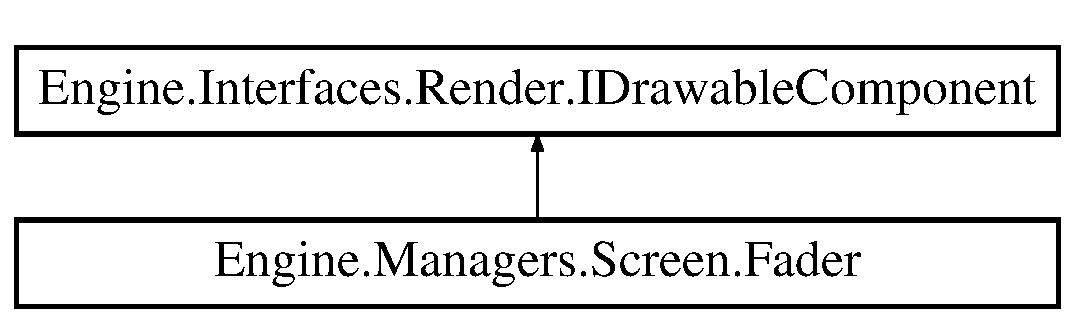
\includegraphics[height=2.000000cm]{dc/d20/a00534}
\end{center}
\end{figure}
\subsection*{Public Member Functions}
\begin{DoxyCompactItemize}
\item 
\hyperlink{a00534_a6dd5b212e90e0c0db26e280c723dcd4f}{Fader} (Vector2 Size)
\begin{DoxyCompactList}\small\item\em C\+O\+N\+S\+T\+R\+U\+C\+T\+OR\+: Sets the basic properties of the fader transition \end{DoxyCompactList}\item 
\hyperlink{a00534_ac33d2bf58aea98d5739f2bb94540be63}{Fader} (Vector2 Size, Vector2 p)
\begin{DoxyCompactList}\small\item\em C\+O\+N\+S\+T\+R\+U\+C\+T\+OR\+: Sets the basic properties of the fader transition \end{DoxyCompactList}\item 
\hyperlink{a00534_ad75a8b6e54b0557b7b463051858524bc}{Fader} (Vector2 Size, Vector2 p, float speed)
\begin{DoxyCompactList}\small\item\em C\+O\+N\+S\+T\+R\+U\+C\+T\+OR\+: Sets the basic properties of the fader transition \end{DoxyCompactList}\item 
void \hyperlink{a00534_a8a40165cf8a910849e01fb35b9567ee2}{Draw} (Sprite\+Batch sb)
\begin{DoxyCompactList}\small\item\em M\+E\+T\+H\+OD\+: Draw the transition \end{DoxyCompactList}\item 
void \hyperlink{a00534_a25631a1ada84786c23242b896dc62692}{Update} ()
\begin{DoxyCompactList}\small\item\em M\+E\+T\+H\+OD\+: The update of the transition which is called every frame \end{DoxyCompactList}\end{DoxyCompactItemize}
\subsection*{Data Fields}
\begin{DoxyCompactItemize}
\item 
bool \hyperlink{a00534_aa2cfb68abbeb910ec086ddb3fc5a06c8}{ready} = false
\begin{DoxyCompactList}\small\item\em D\+E\+C\+L\+A\+RE\+: bool for when the screen is ready to transition \end{DoxyCompactList}\end{DoxyCompactItemize}


\subsection{Constructor \& Destructor Documentation}
\mbox{\Hypertarget{a00534_a6dd5b212e90e0c0db26e280c723dcd4f}\label{a00534_a6dd5b212e90e0c0db26e280c723dcd4f}} 
\index{Engine\+::\+Managers\+::\+Screen\+::\+Fader@{Engine\+::\+Managers\+::\+Screen\+::\+Fader}!Fader@{Fader}}
\index{Fader@{Fader}!Engine\+::\+Managers\+::\+Screen\+::\+Fader@{Engine\+::\+Managers\+::\+Screen\+::\+Fader}}
\subsubsection{\texorpdfstring{Fader()}{Fader()}\hspace{0.1cm}{\footnotesize\ttfamily [1/3]}}
{\footnotesize\ttfamily Engine.\+Managers.\+Screen.\+Fader.\+Fader (\begin{DoxyParamCaption}\item[{Vector2}]{Size }\end{DoxyParamCaption})\hspace{0.3cm}{\ttfamily [inline]}}



C\+O\+N\+S\+T\+R\+U\+C\+T\+OR\+: Sets the basic properties of the fader transition 


\begin{DoxyParams}{Parameters}
{\em Size} & Size, the dimensions of the screen to be covered in the transition\\
\hline
\end{DoxyParams}
S\+ET\+: the texture to a constant black

S\+ET\+: the bounds of the transition screen \mbox{\Hypertarget{a00534_ac33d2bf58aea98d5739f2bb94540be63}\label{a00534_ac33d2bf58aea98d5739f2bb94540be63}} 
\index{Engine\+::\+Managers\+::\+Screen\+::\+Fader@{Engine\+::\+Managers\+::\+Screen\+::\+Fader}!Fader@{Fader}}
\index{Fader@{Fader}!Engine\+::\+Managers\+::\+Screen\+::\+Fader@{Engine\+::\+Managers\+::\+Screen\+::\+Fader}}
\subsubsection{\texorpdfstring{Fader()}{Fader()}\hspace{0.1cm}{\footnotesize\ttfamily [2/3]}}
{\footnotesize\ttfamily Engine.\+Managers.\+Screen.\+Fader.\+Fader (\begin{DoxyParamCaption}\item[{Vector2}]{Size,  }\item[{Vector2}]{p }\end{DoxyParamCaption})\hspace{0.3cm}{\ttfamily [inline]}}



C\+O\+N\+S\+T\+R\+U\+C\+T\+OR\+: Sets the basic properties of the fader transition 


\begin{DoxyParams}{Parameters}
{\em Size} & Size, the dimensions of the screen to be covered in the transition\\
\hline
{\em p} & p, the top left corner of the fade transition\\
\hline
\end{DoxyParams}
S\+ET\+: the texture to a constant black

S\+ET\+: the bounds of the transition screen \mbox{\Hypertarget{a00534_ad75a8b6e54b0557b7b463051858524bc}\label{a00534_ad75a8b6e54b0557b7b463051858524bc}} 
\index{Engine\+::\+Managers\+::\+Screen\+::\+Fader@{Engine\+::\+Managers\+::\+Screen\+::\+Fader}!Fader@{Fader}}
\index{Fader@{Fader}!Engine\+::\+Managers\+::\+Screen\+::\+Fader@{Engine\+::\+Managers\+::\+Screen\+::\+Fader}}
\subsubsection{\texorpdfstring{Fader()}{Fader()}\hspace{0.1cm}{\footnotesize\ttfamily [3/3]}}
{\footnotesize\ttfamily Engine.\+Managers.\+Screen.\+Fader.\+Fader (\begin{DoxyParamCaption}\item[{Vector2}]{Size,  }\item[{Vector2}]{p,  }\item[{float}]{speed }\end{DoxyParamCaption})\hspace{0.3cm}{\ttfamily [inline]}}



C\+O\+N\+S\+T\+R\+U\+C\+T\+OR\+: Sets the basic properties of the fader transition 


\begin{DoxyParams}{Parameters}
{\em Size} & Size, the dimensions of the screen to be covered in the transition\\
\hline
{\em p} & p, the top left corner of the fade transition\\
\hline
{\em speed} & speed, how quickly the screen will fade to and from black\\
\hline
\end{DoxyParams}


\subsection{Member Function Documentation}
\mbox{\Hypertarget{a00534_a8a40165cf8a910849e01fb35b9567ee2}\label{a00534_a8a40165cf8a910849e01fb35b9567ee2}} 
\index{Engine\+::\+Managers\+::\+Screen\+::\+Fader@{Engine\+::\+Managers\+::\+Screen\+::\+Fader}!Draw@{Draw}}
\index{Draw@{Draw}!Engine\+::\+Managers\+::\+Screen\+::\+Fader@{Engine\+::\+Managers\+::\+Screen\+::\+Fader}}
\subsubsection{\texorpdfstring{Draw()}{Draw()}}
{\footnotesize\ttfamily void Engine.\+Managers.\+Screen.\+Fader.\+Draw (\begin{DoxyParamCaption}\item[{Sprite\+Batch}]{sb }\end{DoxyParamCaption})\hspace{0.3cm}{\ttfamily [inline]}}



M\+E\+T\+H\+OD\+: Draw the transition 


\begin{DoxyParams}{Parameters}
{\em sb} & Monogame Sprite\+Batch\\
\hline
\end{DoxyParams}


Implements \hyperlink{a00454_a13aad31e3e179532915dbb93e91afaa3}{Engine.\+Interfaces.\+Render.\+I\+Drawable\+Component}.

\mbox{\Hypertarget{a00534_a25631a1ada84786c23242b896dc62692}\label{a00534_a25631a1ada84786c23242b896dc62692}} 
\index{Engine\+::\+Managers\+::\+Screen\+::\+Fader@{Engine\+::\+Managers\+::\+Screen\+::\+Fader}!Update@{Update}}
\index{Update@{Update}!Engine\+::\+Managers\+::\+Screen\+::\+Fader@{Engine\+::\+Managers\+::\+Screen\+::\+Fader}}
\subsubsection{\texorpdfstring{Update()}{Update()}}
{\footnotesize\ttfamily void Engine.\+Managers.\+Screen.\+Fader.\+Update (\begin{DoxyParamCaption}{ }\end{DoxyParamCaption})\hspace{0.3cm}{\ttfamily [inline]}}



M\+E\+T\+H\+OD\+: The update of the transition which is called every frame 

I\+N\+C\+R\+E\+M\+E\+NT\+: the timer

IF\+: Transitioning in to the fade, increase the alpha making the black box more opaque

E\+L\+SE\+: Transitioning out of the fade, decrease the alpha making the black box less opaque

IF\+: Fully transparent

S\+ET\+: Alpha 0 and ready true

IF\+: Fully Opaque

S\+ET\+: Alpha 1 and transition to Out

Adjust texture 

\subsection{Field Documentation}
\mbox{\Hypertarget{a00534_aa2cfb68abbeb910ec086ddb3fc5a06c8}\label{a00534_aa2cfb68abbeb910ec086ddb3fc5a06c8}} 
\index{Engine\+::\+Managers\+::\+Screen\+::\+Fader@{Engine\+::\+Managers\+::\+Screen\+::\+Fader}!ready@{ready}}
\index{ready@{ready}!Engine\+::\+Managers\+::\+Screen\+::\+Fader@{Engine\+::\+Managers\+::\+Screen\+::\+Fader}}
\subsubsection{\texorpdfstring{ready}{ready}}
{\footnotesize\ttfamily bool Engine.\+Managers.\+Screen.\+Fader.\+ready = false}



D\+E\+C\+L\+A\+RE\+: bool for when the screen is ready to transition 



The documentation for this class was generated from the following file\+:\begin{DoxyCompactItemize}
\item 
\hyperlink{a00182}{Fader.\+cs}\end{DoxyCompactItemize}

\hypertarget{a00306}{}\section{Engine.\+Game1 Class Reference}
\label{a00306}\index{Engine.\+Game1@{Engine.\+Game1}}
Inheritance diagram for Engine.\+Game1\+:\begin{figure}[H]
\begin{center}
\leavevmode
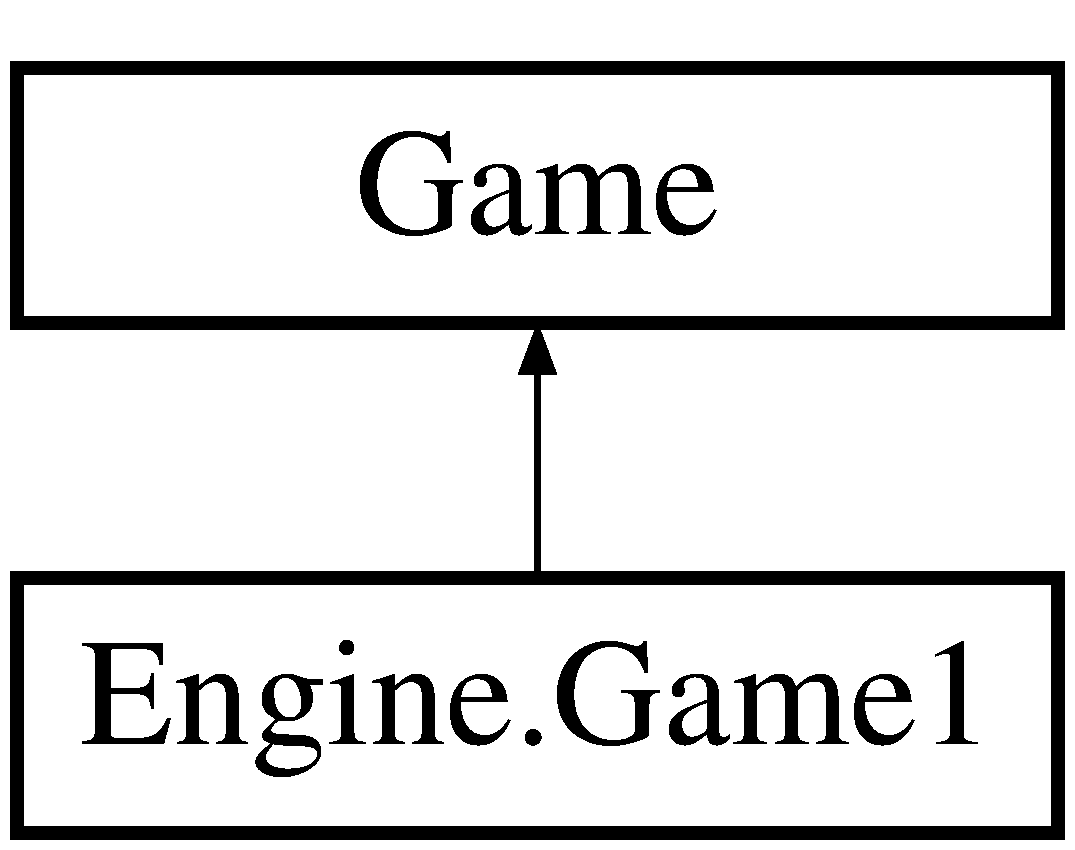
\includegraphics[height=2.000000cm]{d1/de3/a00306}
\end{center}
\end{figure}
\subsection*{Public Member Functions}
\begin{DoxyCompactItemize}
\item 
\hyperlink{a00306_a321d836485b0e6ba049e1200dee17c3b}{Game1} ()
\end{DoxyCompactItemize}
\subsection*{Data Fields}
\begin{DoxyCompactItemize}
\item 
Graphics\+Device\+Manager \hyperlink{a00306_a6080a5540f79b78b6604cba45c3e0817}{graphics}
\end{DoxyCompactItemize}
\subsection*{Static Public Attributes}
\begin{DoxyCompactItemize}
\item 
static \hyperlink{a00306}{Game1} \hyperlink{a00306_a6edc487a30ce1f26309e430b29e25f72}{Instance}
\end{DoxyCompactItemize}
\subsection*{Protected Member Functions}
\begin{DoxyCompactItemize}
\item 
override void \hyperlink{a00306_a640e4df5dfc3ea2b4dab155f3dc3152c}{Initialize} ()
\begin{DoxyCompactList}\small\item\em Initialize;. \end{DoxyCompactList}\item 
override void \hyperlink{a00306_a0c121f8c93986e79a1c402689f53d78e}{Load\+Content} ()
\item 
override void \hyperlink{a00306_a514f0c28029716a22b7e580a06fef9a0}{Unload\+Content} ()
\item 
override void \hyperlink{a00306_a5ec7bcee1272c1a62a77292cd95d043f}{Update} (Game\+Time game\+Time)
\item 
override void \hyperlink{a00306_a0d4254c27d581ec3a459cfc439a1a071}{Draw} (Game\+Time game\+Time)
\end{DoxyCompactItemize}


\subsection{Constructor \& Destructor Documentation}
\mbox{\Hypertarget{a00306_a321d836485b0e6ba049e1200dee17c3b}\label{a00306_a321d836485b0e6ba049e1200dee17c3b}} 
\index{Engine\+::\+Game1@{Engine\+::\+Game1}!Game1@{Game1}}
\index{Game1@{Game1}!Engine\+::\+Game1@{Engine\+::\+Game1}}
\subsubsection{\texorpdfstring{Game1()}{Game1()}}
{\footnotesize\ttfamily Engine.\+Game1.\+Game1 (\begin{DoxyParamCaption}{ }\end{DoxyParamCaption})\hspace{0.3cm}{\ttfamily [inline]}}



\subsection{Member Function Documentation}
\mbox{\Hypertarget{a00306_a0d4254c27d581ec3a459cfc439a1a071}\label{a00306_a0d4254c27d581ec3a459cfc439a1a071}} 
\index{Engine\+::\+Game1@{Engine\+::\+Game1}!Draw@{Draw}}
\index{Draw@{Draw}!Engine\+::\+Game1@{Engine\+::\+Game1}}
\subsubsection{\texorpdfstring{Draw()}{Draw()}}
{\footnotesize\ttfamily override void Engine.\+Game1.\+Draw (\begin{DoxyParamCaption}\item[{Game\+Time}]{game\+Time }\end{DoxyParamCaption})\hspace{0.3cm}{\ttfamily [inline]}, {\ttfamily [protected]}}

Draw Everything \mbox{\Hypertarget{a00306_a640e4df5dfc3ea2b4dab155f3dc3152c}\label{a00306_a640e4df5dfc3ea2b4dab155f3dc3152c}} 
\index{Engine\+::\+Game1@{Engine\+::\+Game1}!Initialize@{Initialize}}
\index{Initialize@{Initialize}!Engine\+::\+Game1@{Engine\+::\+Game1}}
\subsubsection{\texorpdfstring{Initialize()}{Initialize()}}
{\footnotesize\ttfamily override void Engine.\+Game1.\+Initialize (\begin{DoxyParamCaption}{ }\end{DoxyParamCaption})\hspace{0.3cm}{\ttfamily [inline]}, {\ttfamily [protected]}}



Initialize;. 

Set the mous to visible \mbox{\Hypertarget{a00306_a0c121f8c93986e79a1c402689f53d78e}\label{a00306_a0c121f8c93986e79a1c402689f53d78e}} 
\index{Engine\+::\+Game1@{Engine\+::\+Game1}!Load\+Content@{Load\+Content}}
\index{Load\+Content@{Load\+Content}!Engine\+::\+Game1@{Engine\+::\+Game1}}
\subsubsection{\texorpdfstring{Load\+Content()}{LoadContent()}}
{\footnotesize\ttfamily override void Engine.\+Game1.\+Load\+Content (\begin{DoxyParamCaption}{ }\end{DoxyParamCaption})\hspace{0.3cm}{\ttfamily [inline]}, {\ttfamily [protected]}}

Create a new Sprite\+Batch, which can be used to draw textures. \mbox{\Hypertarget{a00306_a514f0c28029716a22b7e580a06fef9a0}\label{a00306_a514f0c28029716a22b7e580a06fef9a0}} 
\index{Engine\+::\+Game1@{Engine\+::\+Game1}!Unload\+Content@{Unload\+Content}}
\index{Unload\+Content@{Unload\+Content}!Engine\+::\+Game1@{Engine\+::\+Game1}}
\subsubsection{\texorpdfstring{Unload\+Content()}{UnloadContent()}}
{\footnotesize\ttfamily override void Engine.\+Game1.\+Unload\+Content (\begin{DoxyParamCaption}{ }\end{DoxyParamCaption})\hspace{0.3cm}{\ttfamily [inline]}, {\ttfamily [protected]}}

T\+O\+DO\+: Unload any non Content\+Manager content here \mbox{\Hypertarget{a00306_a5ec7bcee1272c1a62a77292cd95d043f}\label{a00306_a5ec7bcee1272c1a62a77292cd95d043f}} 
\index{Engine\+::\+Game1@{Engine\+::\+Game1}!Update@{Update}}
\index{Update@{Update}!Engine\+::\+Game1@{Engine\+::\+Game1}}
\subsubsection{\texorpdfstring{Update()}{Update()}}
{\footnotesize\ttfamily override void Engine.\+Game1.\+Update (\begin{DoxyParamCaption}\item[{Game\+Time}]{game\+Time }\end{DoxyParamCaption})\hspace{0.3cm}{\ttfamily [inline]}, {\ttfamily [protected]}}

Not everything has been intergrated to the new input 

\subsection{Field Documentation}
\mbox{\Hypertarget{a00306_a6080a5540f79b78b6604cba45c3e0817}\label{a00306_a6080a5540f79b78b6604cba45c3e0817}} 
\index{Engine\+::\+Game1@{Engine\+::\+Game1}!graphics@{graphics}}
\index{graphics@{graphics}!Engine\+::\+Game1@{Engine\+::\+Game1}}
\subsubsection{\texorpdfstring{graphics}{graphics}}
{\footnotesize\ttfamily Graphics\+Device\+Manager Engine.\+Game1.\+graphics}

List of Update Components List of Draw Components \mbox{\Hypertarget{a00306_a6edc487a30ce1f26309e430b29e25f72}\label{a00306_a6edc487a30ce1f26309e430b29e25f72}} 
\index{Engine\+::\+Game1@{Engine\+::\+Game1}!Instance@{Instance}}
\index{Instance@{Instance}!Engine\+::\+Game1@{Engine\+::\+Game1}}
\subsubsection{\texorpdfstring{Instance}{Instance}}
{\footnotesize\ttfamily \hyperlink{a00306}{Game1} Engine.\+Game1.\+Instance\hspace{0.3cm}{\ttfamily [static]}}



The documentation for this class was generated from the following file\+:\begin{DoxyCompactItemize}
\item 
\hyperlink{a00008}{Game1.\+cs}\end{DoxyCompactItemize}

\hypertarget{a00558}{}\section{Engine.\+States.\+Game\+Options.\+Game\+Options Class Reference}
\label{a00558}\index{Engine.\+States.\+Game\+Options.\+Game\+Options@{Engine.\+States.\+Game\+Options.\+Game\+Options}}


C\+L\+A\+SS\+: The \hyperlink{a00558}{Game\+Options} screen allows the user to adjust settings for the game such as the volume for the game  


Inheritance diagram for Engine.\+States.\+Game\+Options.\+Game\+Options\+:\begin{figure}[H]
\begin{center}
\leavevmode
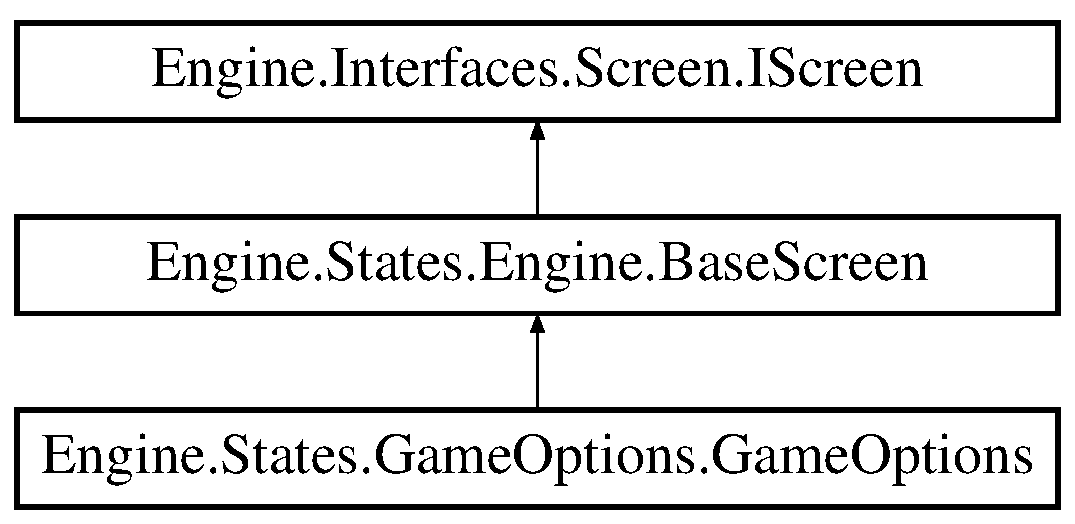
\includegraphics[height=3.000000cm]{dc/dea/a00558}
\end{center}
\end{figure}
\subsection*{Public Member Functions}
\begin{DoxyCompactItemize}
\item 
\hyperlink{a00558_aeea264989e80b36956d21eb8ecd53d07}{Game\+Options} ()
\begin{DoxyCompactList}\small\item\em C\+O\+N\+S\+T\+R\+U\+C\+T\+OR \end{DoxyCompactList}\item 
override void \hyperlink{a00558_a1547a699546baa41aa39a2e2b4412787}{Initialize} ()
\begin{DoxyCompactList}\small\item\em M\+E\+T\+H\+OD\+: Initialisation Logic here \end{DoxyCompactList}\item 
override void \hyperlink{a00558_aedf1c1415b77bf7c8ce37d754039de7b}{Unload} ()
\begin{DoxyCompactList}\small\item\em M\+E\+T\+H\+OD\+: Unload the content of this screen \end{DoxyCompactList}\item 
override void \hyperlink{a00558_a7668c0681e2f3bd52cb65b3abda014bd}{Draw} (Microsoft.\+Xna.\+Framework.\+Graphics.\+Sprite\+Batch sprite\+Batch)
\begin{DoxyCompactList}\small\item\em M\+E\+T\+H\+OD\+: Draw the content of the screen \end{DoxyCompactList}\item 
void \hyperlink{a00558_a595552ae004bb6c7d5d42605c1c5d239}{On\+Key\+Down} (object sender, \hyperlink{a00362}{Key\+Event\+Args} e)
\begin{DoxyCompactList}\small\item\em E\+V\+E\+NT\+: When a key is pressed this event fires \end{DoxyCompactList}\item 
override void \hyperlink{a00558_a629d2a00abd6bfcc21524911e74fee3a}{Update} (Game\+Time game\+Time)
\begin{DoxyCompactList}\small\item\em M\+E\+T\+H\+OD\+: Update is cycled through every frame and contains the logic for updating the screen \end{DoxyCompactList}\end{DoxyCompactItemize}
\subsection*{Additional Inherited Members}


\subsection{Detailed Description}
C\+L\+A\+SS\+: The \hyperlink{a00558}{Game\+Options} screen allows the user to adjust settings for the game such as the volume for the game 



\subsection{Constructor \& Destructor Documentation}
\mbox{\Hypertarget{a00558_aeea264989e80b36956d21eb8ecd53d07}\label{a00558_aeea264989e80b36956d21eb8ecd53d07}} 
\index{Engine\+::\+States\+::\+Game\+Options\+::\+Game\+Options@{Engine\+::\+States\+::\+Game\+Options\+::\+Game\+Options}!Game\+Options@{Game\+Options}}
\index{Game\+Options@{Game\+Options}!Engine\+::\+States\+::\+Game\+Options\+::\+Game\+Options@{Engine\+::\+States\+::\+Game\+Options\+::\+Game\+Options}}
\subsubsection{\texorpdfstring{Game\+Options()}{GameOptions()}}
{\footnotesize\ttfamily Engine.\+States.\+Game\+Options.\+Game\+Options.\+Game\+Options (\begin{DoxyParamCaption}{ }\end{DoxyParamCaption})\hspace{0.3cm}{\ttfamily [inline]}}



C\+O\+N\+S\+T\+R\+U\+C\+T\+OR 



\subsection{Member Function Documentation}
\mbox{\Hypertarget{a00558_a7668c0681e2f3bd52cb65b3abda014bd}\label{a00558_a7668c0681e2f3bd52cb65b3abda014bd}} 
\index{Engine\+::\+States\+::\+Game\+Options\+::\+Game\+Options@{Engine\+::\+States\+::\+Game\+Options\+::\+Game\+Options}!Draw@{Draw}}
\index{Draw@{Draw}!Engine\+::\+States\+::\+Game\+Options\+::\+Game\+Options@{Engine\+::\+States\+::\+Game\+Options\+::\+Game\+Options}}
\subsubsection{\texorpdfstring{Draw()}{Draw()}}
{\footnotesize\ttfamily override void Engine.\+States.\+Game\+Options.\+Game\+Options.\+Draw (\begin{DoxyParamCaption}\item[{Microsoft.\+Xna.\+Framework.\+Graphics.\+Sprite\+Batch}]{sprite\+Batch }\end{DoxyParamCaption})\hspace{0.3cm}{\ttfamily [inline]}}



M\+E\+T\+H\+OD\+: Draw the content of the screen 


\begin{DoxyParams}{Parameters}
{\em sprite\+Batch} & Mono\+Game Sprite\+Batch\\
\hline
\end{DoxyParams}
\mbox{\Hypertarget{a00558_a1547a699546baa41aa39a2e2b4412787}\label{a00558_a1547a699546baa41aa39a2e2b4412787}} 
\index{Engine\+::\+States\+::\+Game\+Options\+::\+Game\+Options@{Engine\+::\+States\+::\+Game\+Options\+::\+Game\+Options}!Initialize@{Initialize}}
\index{Initialize@{Initialize}!Engine\+::\+States\+::\+Game\+Options\+::\+Game\+Options@{Engine\+::\+States\+::\+Game\+Options\+::\+Game\+Options}}
\subsubsection{\texorpdfstring{Initialize()}{Initialize()}}
{\footnotesize\ttfamily override void Engine.\+States.\+Game\+Options.\+Game\+Options.\+Initialize (\begin{DoxyParamCaption}{ }\end{DoxyParamCaption})\hspace{0.3cm}{\ttfamily [inline]}, {\ttfamily [virtual]}}



M\+E\+T\+H\+OD\+: Initialisation Logic here 

S\+ET\+: Soundtrack

C\+A\+LL\+: Base\+Screen initialize

E\+V\+E\+NT\+: Add a key\+Down event

I\+N\+I\+T\+I\+A\+L\+I\+SE\+: the menu options

D\+E\+C\+L\+A\+RE\+: the y\+Offset for the gap between options

Cycle through the list of options and add them to the screen 

Reimplemented from \hyperlink{a00550_af8fd6890abf865641e190578ef2e054c}{Engine.\+States.\+Engine.\+Base\+Screen}.

\mbox{\Hypertarget{a00558_a595552ae004bb6c7d5d42605c1c5d239}\label{a00558_a595552ae004bb6c7d5d42605c1c5d239}} 
\index{Engine\+::\+States\+::\+Game\+Options\+::\+Game\+Options@{Engine\+::\+States\+::\+Game\+Options\+::\+Game\+Options}!On\+Key\+Down@{On\+Key\+Down}}
\index{On\+Key\+Down@{On\+Key\+Down}!Engine\+::\+States\+::\+Game\+Options\+::\+Game\+Options@{Engine\+::\+States\+::\+Game\+Options\+::\+Game\+Options}}
\subsubsection{\texorpdfstring{On\+Key\+Down()}{OnKeyDown()}}
{\footnotesize\ttfamily void Engine.\+States.\+Game\+Options.\+Game\+Options.\+On\+Key\+Down (\begin{DoxyParamCaption}\item[{object}]{sender,  }\item[{\hyperlink{a00362}{Key\+Event\+Args}}]{e }\end{DoxyParamCaption})\hspace{0.3cm}{\ttfamily [inline]}}



E\+V\+E\+NT\+: When a key is pressed this event fires 


\begin{DoxyParams}{Parameters}
{\em sender} & \\
\hline
{\em e} & \\
\hline
\end{DoxyParams}
IF\+: Enter key is pressed

S\+W\+I\+T\+CH\+: adjust options as necessary

Mute sound if unmuted, otherwise unmute it

Switch between Fullscreen and windowed mode

IF\+: + is pressed, increase volume if also on the volume options

IF\+: -\/ is pressed, decrease volume if also on the volume options

IF\+: Up is pressed, move backwards through the list

IF\+: Down is pressed, move forwards through the list \mbox{\Hypertarget{a00558_aedf1c1415b77bf7c8ce37d754039de7b}\label{a00558_aedf1c1415b77bf7c8ce37d754039de7b}} 
\index{Engine\+::\+States\+::\+Game\+Options\+::\+Game\+Options@{Engine\+::\+States\+::\+Game\+Options\+::\+Game\+Options}!Unload@{Unload}}
\index{Unload@{Unload}!Engine\+::\+States\+::\+Game\+Options\+::\+Game\+Options@{Engine\+::\+States\+::\+Game\+Options\+::\+Game\+Options}}
\subsubsection{\texorpdfstring{Unload()}{Unload()}}
{\footnotesize\ttfamily override void Engine.\+States.\+Game\+Options.\+Game\+Options.\+Unload (\begin{DoxyParamCaption}{ }\end{DoxyParamCaption})\hspace{0.3cm}{\ttfamily [inline]}, {\ttfamily [virtual]}}



M\+E\+T\+H\+OD\+: Unload the content of this screen 



Reimplemented from \hyperlink{a00550_a861ab6364e68e3e3b6b9718e34ba18a2}{Engine.\+States.\+Engine.\+Base\+Screen}.

\mbox{\Hypertarget{a00558_a629d2a00abd6bfcc21524911e74fee3a}\label{a00558_a629d2a00abd6bfcc21524911e74fee3a}} 
\index{Engine\+::\+States\+::\+Game\+Options\+::\+Game\+Options@{Engine\+::\+States\+::\+Game\+Options\+::\+Game\+Options}!Update@{Update}}
\index{Update@{Update}!Engine\+::\+States\+::\+Game\+Options\+::\+Game\+Options@{Engine\+::\+States\+::\+Game\+Options\+::\+Game\+Options}}
\subsubsection{\texorpdfstring{Update()}{Update()}}
{\footnotesize\ttfamily override void Engine.\+States.\+Game\+Options.\+Game\+Options.\+Update (\begin{DoxyParamCaption}\item[{Game\+Time}]{game\+Time }\end{DoxyParamCaption})\hspace{0.3cm}{\ttfamily [inline]}, {\ttfamily [virtual]}}



M\+E\+T\+H\+OD\+: Update is cycled through every frame and contains the logic for updating the screen 


\begin{DoxyParams}{Parameters}
{\em game\+Time} & \\
\hline
\end{DoxyParams}
F\+O\+R\+E\+A\+CH\+: \hyperlink{a00578}{Menu\+Item}, if currently selected, set bool appropriately 

Reimplemented from \hyperlink{a00550_a098ece7d1e112475f6e880c3a672af64}{Engine.\+States.\+Engine.\+Base\+Screen}.



The documentation for this class was generated from the following file\+:\begin{DoxyCompactItemize}
\item 
\hyperlink{a00200}{Game\+Options.\+cs}\end{DoxyCompactItemize}

\hypertarget{a00598}{}\section{Engine.\+Utilities.\+Game\+Text Class Reference}
\label{a00598}\index{Engine.\+Utilities.\+Game\+Text@{Engine.\+Utilities.\+Game\+Text}}
\subsection*{Public Member Functions}
\begin{DoxyCompactItemize}
\item 
\hyperlink{a00598_adcd7d2f1e49ae060840835d804958686}{Game\+Text} (string text, string font, Vector2 pos, Color color, float size)
\item 
void \hyperlink{a00598_aa89cba517208148817587ad1bf6a4855}{Draw} (Sprite\+Batch spr)
\end{DoxyCompactItemize}


\subsection{Constructor \& Destructor Documentation}
\mbox{\Hypertarget{a00598_adcd7d2f1e49ae060840835d804958686}\label{a00598_adcd7d2f1e49ae060840835d804958686}} 
\index{Engine\+::\+Utilities\+::\+Game\+Text@{Engine\+::\+Utilities\+::\+Game\+Text}!Game\+Text@{Game\+Text}}
\index{Game\+Text@{Game\+Text}!Engine\+::\+Utilities\+::\+Game\+Text@{Engine\+::\+Utilities\+::\+Game\+Text}}
\subsubsection{\texorpdfstring{Game\+Text()}{GameText()}}
{\footnotesize\ttfamily Engine.\+Utilities.\+Game\+Text.\+Game\+Text (\begin{DoxyParamCaption}\item[{string}]{text,  }\item[{string}]{font,  }\item[{Vector2}]{pos,  }\item[{Color}]{color,  }\item[{float}]{size }\end{DoxyParamCaption})\hspace{0.3cm}{\ttfamily [inline]}}



\subsection{Member Function Documentation}
\mbox{\Hypertarget{a00598_aa89cba517208148817587ad1bf6a4855}\label{a00598_aa89cba517208148817587ad1bf6a4855}} 
\index{Engine\+::\+Utilities\+::\+Game\+Text@{Engine\+::\+Utilities\+::\+Game\+Text}!Draw@{Draw}}
\index{Draw@{Draw}!Engine\+::\+Utilities\+::\+Game\+Text@{Engine\+::\+Utilities\+::\+Game\+Text}}
\subsubsection{\texorpdfstring{Draw()}{Draw()}}
{\footnotesize\ttfamily void Engine.\+Utilities.\+Game\+Text.\+Draw (\begin{DoxyParamCaption}\item[{Sprite\+Batch}]{spr }\end{DoxyParamCaption})\hspace{0.3cm}{\ttfamily [inline]}}



The documentation for this class was generated from the following file\+:\begin{DoxyCompactItemize}
\item 
\hyperlink{a00230}{Game\+Text.\+cs}\end{DoxyCompactItemize}

\hypertarget{a00406}{}\section{Engine.\+Grid.\+Grids Class Reference}
\label{a00406}\index{Engine.\+Grid.\+Grids@{Engine.\+Grid.\+Grids}}
\subsection*{Public Member Functions}
\begin{DoxyCompactItemize}
\item 
\hyperlink{a00406_a93c6400681153abcf5bf341f72e77277}{Grids} (Texture2D tex)
\item 
void \hyperlink{a00406_a42a73fb81510d705071435c621d12c72}{create} (int X, int Y)
\item 
void \hyperlink{a00406_abaa6e136966cf7c17141a042c5ac1d71}{do\+Stuff} ()
\item 
void \hyperlink{a00406_aec9a6ddb83a21aa1e3ef16dc8cae4808}{setup\+Visual} ()
\item 
void \hyperlink{a00406_a036d69651829420e4494004d9cf73b71}{reset\+Visual} ()
\item 
void \hyperlink{a00406_ab0cc24116dc6df9c8d0acdc6b0d51b0d}{set\+Node\+Positions} (int width, int height)
\item 
void \hyperlink{a00406_ab8bebc68904ff66b2a10832f2540e188}{Draw} (Sprite\+Batch sb)
\item 
List$<$ \hyperlink{a00414}{Node} $>$ \hyperlink{a00406_a3380ff062497543fe12b24a0e3ddfc46}{get\+Neighbours} (\hyperlink{a00414}{Node} check)
\item 
bool \hyperlink{a00406_a0f0825c55c7d8a17b163f74fc8baa9de}{check\+Map} (int x, int y)
\end{DoxyCompactItemize}
\subsection*{Data Fields}
\begin{DoxyCompactItemize}
\item 
List$<$ \hyperlink{a00414}{Node} $>$ \hyperlink{a00406_ad9776283305f0c420d4a544d418a7c40}{path} = new List$<$\hyperlink{a00414}{Node}$>$()
\end{DoxyCompactItemize}
\subsection*{Properties}
\begin{DoxyCompactItemize}
\item 
\hyperlink{a00414}{Node} \mbox{[},\mbox{]} \hyperlink{a00406_a272de0996ab650f3dde958644d26b032}{get\+Grid}\hspace{0.3cm}{\ttfamily  \mbox{[}get\mbox{]}}
\end{DoxyCompactItemize}


\subsection{Constructor \& Destructor Documentation}
\mbox{\Hypertarget{a00406_a93c6400681153abcf5bf341f72e77277}\label{a00406_a93c6400681153abcf5bf341f72e77277}} 
\index{Engine\+::\+Grid\+::\+Grids@{Engine\+::\+Grid\+::\+Grids}!Grids@{Grids}}
\index{Grids@{Grids}!Engine\+::\+Grid\+::\+Grids@{Engine\+::\+Grid\+::\+Grids}}
\subsubsection{\texorpdfstring{Grids()}{Grids()}}
{\footnotesize\ttfamily Engine.\+Grid.\+Grids.\+Grids (\begin{DoxyParamCaption}\item[{Texture2D}]{tex }\end{DoxyParamCaption})\hspace{0.3cm}{\ttfamily [inline]}}



\subsection{Member Function Documentation}
\mbox{\Hypertarget{a00406_a0f0825c55c7d8a17b163f74fc8baa9de}\label{a00406_a0f0825c55c7d8a17b163f74fc8baa9de}} 
\index{Engine\+::\+Grid\+::\+Grids@{Engine\+::\+Grid\+::\+Grids}!check\+Map@{check\+Map}}
\index{check\+Map@{check\+Map}!Engine\+::\+Grid\+::\+Grids@{Engine\+::\+Grid\+::\+Grids}}
\subsubsection{\texorpdfstring{check\+Map()}{checkMap()}}
{\footnotesize\ttfamily bool Engine.\+Grid.\+Grids.\+check\+Map (\begin{DoxyParamCaption}\item[{int}]{x,  }\item[{int}]{y }\end{DoxyParamCaption})\hspace{0.3cm}{\ttfamily [inline]}}

\mbox{\Hypertarget{a00406_a42a73fb81510d705071435c621d12c72}\label{a00406_a42a73fb81510d705071435c621d12c72}} 
\index{Engine\+::\+Grid\+::\+Grids@{Engine\+::\+Grid\+::\+Grids}!create@{create}}
\index{create@{create}!Engine\+::\+Grid\+::\+Grids@{Engine\+::\+Grid\+::\+Grids}}
\subsubsection{\texorpdfstring{create()}{create()}}
{\footnotesize\ttfamily void Engine.\+Grid.\+Grids.\+create (\begin{DoxyParamCaption}\item[{int}]{X,  }\item[{int}]{Y }\end{DoxyParamCaption})\hspace{0.3cm}{\ttfamily [inline]}}

\mbox{\Hypertarget{a00406_abaa6e136966cf7c17141a042c5ac1d71}\label{a00406_abaa6e136966cf7c17141a042c5ac1d71}} 
\index{Engine\+::\+Grid\+::\+Grids@{Engine\+::\+Grid\+::\+Grids}!do\+Stuff@{do\+Stuff}}
\index{do\+Stuff@{do\+Stuff}!Engine\+::\+Grid\+::\+Grids@{Engine\+::\+Grid\+::\+Grids}}
\subsubsection{\texorpdfstring{do\+Stuff()}{doStuff()}}
{\footnotesize\ttfamily void Engine.\+Grid.\+Grids.\+do\+Stuff (\begin{DoxyParamCaption}{ }\end{DoxyParamCaption})\hspace{0.3cm}{\ttfamily [inline]}}

Console.\+Write\+Line(\char`\"{}neighbour X \char`\"{} + neigh\mbox{[}i\mbox{]}.get\+Grid.\+X + \char`\"{} \char`\"{} + \char`\"{} Neighbour Y\char`\"{} + neigh\mbox{[}i\mbox{]}.get\+Grid.\+Y); \mbox{\Hypertarget{a00406_ab8bebc68904ff66b2a10832f2540e188}\label{a00406_ab8bebc68904ff66b2a10832f2540e188}} 
\index{Engine\+::\+Grid\+::\+Grids@{Engine\+::\+Grid\+::\+Grids}!Draw@{Draw}}
\index{Draw@{Draw}!Engine\+::\+Grid\+::\+Grids@{Engine\+::\+Grid\+::\+Grids}}
\subsubsection{\texorpdfstring{Draw()}{Draw()}}
{\footnotesize\ttfamily void Engine.\+Grid.\+Grids.\+Draw (\begin{DoxyParamCaption}\item[{Sprite\+Batch}]{sb }\end{DoxyParamCaption})\hspace{0.3cm}{\ttfamily [inline]}}

\mbox{\Hypertarget{a00406_a3380ff062497543fe12b24a0e3ddfc46}\label{a00406_a3380ff062497543fe12b24a0e3ddfc46}} 
\index{Engine\+::\+Grid\+::\+Grids@{Engine\+::\+Grid\+::\+Grids}!get\+Neighbours@{get\+Neighbours}}
\index{get\+Neighbours@{get\+Neighbours}!Engine\+::\+Grid\+::\+Grids@{Engine\+::\+Grid\+::\+Grids}}
\subsubsection{\texorpdfstring{get\+Neighbours()}{getNeighbours()}}
{\footnotesize\ttfamily List$<$\hyperlink{a00414}{Node}$>$ Engine.\+Grid.\+Grids.\+get\+Neighbours (\begin{DoxyParamCaption}\item[{\hyperlink{a00414}{Node}}]{check }\end{DoxyParamCaption})\hspace{0.3cm}{\ttfamily [inline]}}

\mbox{\Hypertarget{a00406_a036d69651829420e4494004d9cf73b71}\label{a00406_a036d69651829420e4494004d9cf73b71}} 
\index{Engine\+::\+Grid\+::\+Grids@{Engine\+::\+Grid\+::\+Grids}!reset\+Visual@{reset\+Visual}}
\index{reset\+Visual@{reset\+Visual}!Engine\+::\+Grid\+::\+Grids@{Engine\+::\+Grid\+::\+Grids}}
\subsubsection{\texorpdfstring{reset\+Visual()}{resetVisual()}}
{\footnotesize\ttfamily void Engine.\+Grid.\+Grids.\+reset\+Visual (\begin{DoxyParamCaption}{ }\end{DoxyParamCaption})\hspace{0.3cm}{\ttfamily [inline]}}

\mbox{\Hypertarget{a00406_ab0cc24116dc6df9c8d0acdc6b0d51b0d}\label{a00406_ab0cc24116dc6df9c8d0acdc6b0d51b0d}} 
\index{Engine\+::\+Grid\+::\+Grids@{Engine\+::\+Grid\+::\+Grids}!set\+Node\+Positions@{set\+Node\+Positions}}
\index{set\+Node\+Positions@{set\+Node\+Positions}!Engine\+::\+Grid\+::\+Grids@{Engine\+::\+Grid\+::\+Grids}}
\subsubsection{\texorpdfstring{set\+Node\+Positions()}{setNodePositions()}}
{\footnotesize\ttfamily void Engine.\+Grid.\+Grids.\+set\+Node\+Positions (\begin{DoxyParamCaption}\item[{int}]{width,  }\item[{int}]{height }\end{DoxyParamCaption})\hspace{0.3cm}{\ttfamily [inline]}}

\mbox{\Hypertarget{a00406_aec9a6ddb83a21aa1e3ef16dc8cae4808}\label{a00406_aec9a6ddb83a21aa1e3ef16dc8cae4808}} 
\index{Engine\+::\+Grid\+::\+Grids@{Engine\+::\+Grid\+::\+Grids}!setup\+Visual@{setup\+Visual}}
\index{setup\+Visual@{setup\+Visual}!Engine\+::\+Grid\+::\+Grids@{Engine\+::\+Grid\+::\+Grids}}
\subsubsection{\texorpdfstring{setup\+Visual()}{setupVisual()}}
{\footnotesize\ttfamily void Engine.\+Grid.\+Grids.\+setup\+Visual (\begin{DoxyParamCaption}{ }\end{DoxyParamCaption})\hspace{0.3cm}{\ttfamily [inline]}}

Increase next X pos by texture width

set x\+Var to 0 because we are done setting x positions

Same for Y 

\subsection{Field Documentation}
\mbox{\Hypertarget{a00406_ad9776283305f0c420d4a544d418a7c40}\label{a00406_ad9776283305f0c420d4a544d418a7c40}} 
\index{Engine\+::\+Grid\+::\+Grids@{Engine\+::\+Grid\+::\+Grids}!path@{path}}
\index{path@{path}!Engine\+::\+Grid\+::\+Grids@{Engine\+::\+Grid\+::\+Grids}}
\subsubsection{\texorpdfstring{path}{path}}
{\footnotesize\ttfamily List$<$\hyperlink{a00414}{Node}$>$ Engine.\+Grid.\+Grids.\+path = new List$<$\hyperlink{a00414}{Node}$>$()}



\subsection{Property Documentation}
\mbox{\Hypertarget{a00406_a272de0996ab650f3dde958644d26b032}\label{a00406_a272de0996ab650f3dde958644d26b032}} 
\index{Engine\+::\+Grid\+::\+Grids@{Engine\+::\+Grid\+::\+Grids}!get\+Grid@{get\+Grid}}
\index{get\+Grid@{get\+Grid}!Engine\+::\+Grid\+::\+Grids@{Engine\+::\+Grid\+::\+Grids}}
\subsubsection{\texorpdfstring{get\+Grid}{getGrid}}
{\footnotesize\ttfamily \hyperlink{a00414}{Node} \mbox{[},\mbox{]} Engine.\+Grid.\+Grids.\+get\+Grid\hspace{0.3cm}{\ttfamily [get]}}



The documentation for this class was generated from the following file\+:\begin{DoxyCompactItemize}
\item 
\hyperlink{a00086}{Grid.\+cs}\end{DoxyCompactItemize}

\hypertarget{a00506}{}\section{Engine.\+Managers.\+Collision.\+Hitbox Class Reference}
\label{a00506}\index{Engine.\+Managers.\+Collision.\+Hitbox@{Engine.\+Managers.\+Collision.\+Hitbox}}


C\+L\+A\+SS\+: Hitboxes that make up the boundaries for each entity to allow for S\+AT collision to work. Each hitbox covers a portion of the texture of an entity and is stored in a List of Hitboxes inside the entity class.  


Inheritance diagram for Engine.\+Managers.\+Collision.\+Hitbox\+:\begin{figure}[H]
\begin{center}
\leavevmode
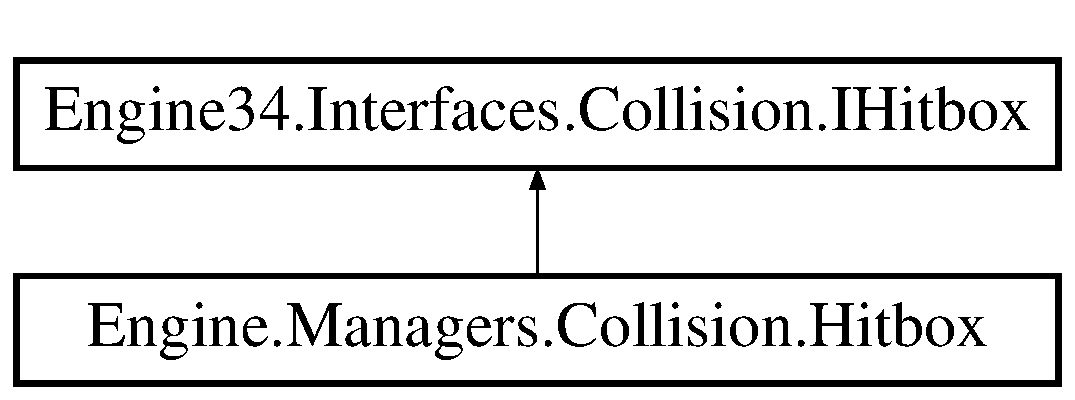
\includegraphics[height=2.000000cm]{d4/d1f/a00506}
\end{center}
\end{figure}
\subsection*{Public Member Functions}
\begin{DoxyCompactItemize}
\item 
\hyperlink{a00506_a0dd1189ee2d37a3401501ca1f10b9cfa}{Hitbox} (Vector2 \+\_\+pos, float p\+Width, float p\+Height, float p\+Rot, \hyperlink{a00318}{Mind} parent)
\begin{DoxyCompactList}\small\item\em C\+O\+N\+S\+T\+R\+U\+C\+T\+OR\+: Takes 5 parameters used to create the List of points and edges and then a rotation used for rotating the shape as necessary to allow for advanced S\+AT \hyperlink{a00268}{Collision} \end{DoxyCompactList}\item 
void \hyperlink{a00506_ab91473c67469cf0be5069c1ca9a2d6fb}{create\+Matrix} ()
\begin{DoxyCompactList}\small\item\em M\+E\+T\+H\+OD\+: A method used to rotate the 4 corners of the shape so that our S\+AT is not just limited to two axes. \end{DoxyCompactList}\item 
Vector2 \hyperlink{a00506_ae78ae27deafc11bf87c1396c504ce621}{create\+Rotation} (Vector2 \+\_\+point)
\begin{DoxyCompactList}\small\item\em M\+E\+T\+H\+OD\+: Rotates a Vector2 around a centre point. The parameter is the point being rotated. In order to rotate the co-\/ordinates around the centre of the shape we must subtract the origin of the rotation from the co-\/ordinate and then add it back on, essentially \char`\"{}moving the object and moving it back\char`\"{}. \end{DoxyCompactList}\item 
void \hyperlink{a00506_a6bc6facadaf82a8c49979e35f0c8b132}{Create\+Edges} ()
\begin{DoxyCompactList}\small\item\em M\+E\+T\+H\+OD\+: Creates edges of the shape by subtracting the previous point if one were to trace the outline of the shape \end{DoxyCompactList}\item 
void \hyperlink{a00506_ab5cba73c16189f63616a91cf19f00562}{Update\+Point} (Vector2 \hyperlink{a00506_a4bfe4a9151e1af19d18f92b4cfba46b6}{velocity})
\begin{DoxyCompactList}\small\item\em M\+E\+T\+H\+OD\+: This is used to move the hitboxes with their parent entities. If this is not done then the collision will not work because the hitbox hasn\textquotesingle{}t moved. \end{DoxyCompactList}\item 
Vector2 \hyperlink{a00506_ad129f58518e4fedffc47433af729b3bf}{centre\+Point} ()
\begin{DoxyCompactList}\small\item\em M\+E\+T\+H\+OD\+: The centre point of the shape. Used for the rotation and for calculating the Minimum Translation Vector When colliding with another \hyperlink{a00506}{Hitbox}. \end{DoxyCompactList}\item 
virtual void \hyperlink{a00506_a987b7fd544e03a9e43e38cc2df785d1d}{Update} ()
\end{DoxyCompactItemize}
\subsection*{Protected Attributes}
\begin{DoxyCompactItemize}
\item 
List$<$ Vector2 $>$ \hyperlink{a00506_ad49c6d92bbdffabb12c2a7a4c7fa3840}{points}
\item 
List$<$ Vector2 $>$ \hyperlink{a00506_a4128afb1364d3a25e1091055ef46dda2}{edges}
\item 
Vector2 \hyperlink{a00506_a4bfe4a9151e1af19d18f92b4cfba46b6}{velocity}
\begin{DoxyCompactList}\small\item\em R\+E\+T\+U\+RN\+: A Vector2 co-\/ordinate of the Velocity of the shape and set the local variable to this property. \end{DoxyCompactList}\item 
\hyperlink{a00446}{I\+Mind} \hyperlink{a00506_a46b5b73419f520327a67808cd768a666}{\+\_\+mind}
\begin{DoxyCompactList}\small\item\em D\+E\+C\+L\+A\+RE\+: A reference to the mind. \end{DoxyCompactList}\end{DoxyCompactItemize}
\subsection*{Properties}
\begin{DoxyCompactItemize}
\item 
List$<$ Vector2 $>$ \hyperlink{a00506_ab706c341cd6e2ba930e2ffe437b6d9c7}{Points}\hspace{0.3cm}{\ttfamily  \mbox{[}get, set\mbox{]}}
\begin{DoxyCompactList}\small\item\em R\+E\+T\+U\+RN\+: A list of a Vector2 co-\/ordinates of the corners of the shape and set the local variable to this property. \end{DoxyCompactList}\item 
List$<$ Vector2 $>$ \hyperlink{a00506_a32ea07f46a9cd6213e965f837758e674}{Edges}\hspace{0.3cm}{\ttfamily  \mbox{[}get, set\mbox{]}}
\begin{DoxyCompactList}\small\item\em R\+E\+T\+U\+RN\+: A list of a Vector2 co-\/ordinates of the edges of the shape and set the local variable to this property. \end{DoxyCompactList}\item 
Vector2 \hyperlink{a00506_a1f0b9781e3ca7fb87c8f9d03080e9f16}{Velocity}\hspace{0.3cm}{\ttfamily  \mbox{[}get, set\mbox{]}}
\item 
\hyperlink{a00446}{I\+Mind} \hyperlink{a00506_a375df917b377e1511e6accd4018a2c30}{Mind}\hspace{0.3cm}{\ttfamily  \mbox{[}get, set\mbox{]}}
\item 
Vector2 \hyperlink{a00506_aea24a643fe9a06c65064bf091427c2fc}{Centre}\hspace{0.3cm}{\ttfamily  \mbox{[}get, set\mbox{]}}
\end{DoxyCompactItemize}


\subsection{Detailed Description}
C\+L\+A\+SS\+: Hitboxes that make up the boundaries for each entity to allow for S\+AT collision to work. Each hitbox covers a portion of the texture of an entity and is stored in a List of Hitboxes inside the entity class. 



\subsection{Constructor \& Destructor Documentation}
\mbox{\Hypertarget{a00506_a0dd1189ee2d37a3401501ca1f10b9cfa}\label{a00506_a0dd1189ee2d37a3401501ca1f10b9cfa}} 
\index{Engine\+::\+Managers\+::\+Collision\+::\+Hitbox@{Engine\+::\+Managers\+::\+Collision\+::\+Hitbox}!Hitbox@{Hitbox}}
\index{Hitbox@{Hitbox}!Engine\+::\+Managers\+::\+Collision\+::\+Hitbox@{Engine\+::\+Managers\+::\+Collision\+::\+Hitbox}}
\subsubsection{\texorpdfstring{Hitbox()}{Hitbox()}}
{\footnotesize\ttfamily Engine.\+Managers.\+Collision.\+Hitbox.\+Hitbox (\begin{DoxyParamCaption}\item[{Vector2}]{\+\_\+pos,  }\item[{float}]{p\+Width,  }\item[{float}]{p\+Height,  }\item[{float}]{p\+Rot,  }\item[{\hyperlink{a00318}{Mind}}]{parent }\end{DoxyParamCaption})\hspace{0.3cm}{\ttfamily [inline]}}



C\+O\+N\+S\+T\+R\+U\+C\+T\+OR\+: Takes 5 parameters used to create the List of points and edges and then a rotation used for rotating the shape as necessary to allow for advanced S\+AT \hyperlink{a00268}{Collision} 


\begin{DoxyParams}{Parameters}
{\em \+\_\+pos} & The position of the first point\\
\hline
{\em p\+Width} & The width of the shape\\
\hline
{\em p\+Height} & The height of the shape\\
\hline
{\em p\+Rot} & The rotation in degrees of the shape\\
\hline
{\em parent} & The mind that this hitox is linked to\\
\hline
\end{DoxyParams}
S\+ET\+: The dimensions of the shape

I\+N\+I\+T\+I\+A\+L\+I\+SE\+: The lists of Vector2 used for the creation of the shape

A\+DD\+: 4 Vector2 co-\/ordinates to the list of points based on the dimensions of the shape and the position

I\+N\+I\+T\+I\+A\+L\+I\+SE\+: The centre point using the method \hyperlink{a00506_ad129f58518e4fedffc47433af729b3bf}{centre\+Point()}

R\+O\+T\+A\+TE\+: Rotate the vector2 for the centre of the shape

R\+O\+T\+A\+TE\+: Call the method to rotate each corner of the shape around the Centre of the shape

C\+R\+E\+A\+TE\+: The edges of the shape by subtracting Corners from each other

S\+ET\+: The mind that controls this hitbox, used for the movement of the Hitboxes. 

\subsection{Member Function Documentation}
\mbox{\Hypertarget{a00506_ad129f58518e4fedffc47433af729b3bf}\label{a00506_ad129f58518e4fedffc47433af729b3bf}} 
\index{Engine\+::\+Managers\+::\+Collision\+::\+Hitbox@{Engine\+::\+Managers\+::\+Collision\+::\+Hitbox}!centre\+Point@{centre\+Point}}
\index{centre\+Point@{centre\+Point}!Engine\+::\+Managers\+::\+Collision\+::\+Hitbox@{Engine\+::\+Managers\+::\+Collision\+::\+Hitbox}}
\subsubsection{\texorpdfstring{centre\+Point()}{centrePoint()}}
{\footnotesize\ttfamily Vector2 Engine.\+Managers.\+Collision.\+Hitbox.\+centre\+Point (\begin{DoxyParamCaption}{ }\end{DoxyParamCaption})\hspace{0.3cm}{\ttfamily [inline]}}



M\+E\+T\+H\+OD\+: The centre point of the shape. Used for the rotation and for calculating the Minimum Translation Vector When colliding with another \hyperlink{a00506}{Hitbox}. 

\begin{DoxyReturn}{Returns}
A Vector2 of the Central co-\/ordinate between all of the points.
\end{DoxyReturn}
x coordinate for the first entity

y coordinate for the first entity

making coordinates into a new vector for the first entity 

Implements \hyperlink{a00434_a5028f79a4e2537e578c528c932dee948}{Engine34.\+Interfaces.\+Collision.\+I\+Hitbox}.

\mbox{\Hypertarget{a00506_a6bc6facadaf82a8c49979e35f0c8b132}\label{a00506_a6bc6facadaf82a8c49979e35f0c8b132}} 
\index{Engine\+::\+Managers\+::\+Collision\+::\+Hitbox@{Engine\+::\+Managers\+::\+Collision\+::\+Hitbox}!Create\+Edges@{Create\+Edges}}
\index{Create\+Edges@{Create\+Edges}!Engine\+::\+Managers\+::\+Collision\+::\+Hitbox@{Engine\+::\+Managers\+::\+Collision\+::\+Hitbox}}
\subsubsection{\texorpdfstring{Create\+Edges()}{CreateEdges()}}
{\footnotesize\ttfamily void Engine.\+Managers.\+Collision.\+Hitbox.\+Create\+Edges (\begin{DoxyParamCaption}{ }\end{DoxyParamCaption})\hspace{0.3cm}{\ttfamily [inline]}}



M\+E\+T\+H\+OD\+: Creates edges of the shape by subtracting the previous point if one were to trace the outline of the shape 

D\+E\+C\+L\+A\+RE\+: Two Vector2 co-\/ordinates

For each point the shape currently has

S\+ET\+: the first point to be the point currently being iterated through in the list.

IF\+: the next point would give an Index\+Out\+Of\+Range Exception

S\+ET\+: the next point to be equal to the first point in the list.

E\+L\+SE\+: The next point is equal to the next one in the list.

C\+R\+E\+A\+TE\+: an Edge by subtracting the second point from the first. This gives us a Vector2 of the translation Between two points. 

Implements \hyperlink{a00434_a94297321cbc20a7cb6a98cf38b735a5b}{Engine34.\+Interfaces.\+Collision.\+I\+Hitbox}.

\mbox{\Hypertarget{a00506_ab91473c67469cf0be5069c1ca9a2d6fb}\label{a00506_ab91473c67469cf0be5069c1ca9a2d6fb}} 
\index{Engine\+::\+Managers\+::\+Collision\+::\+Hitbox@{Engine\+::\+Managers\+::\+Collision\+::\+Hitbox}!create\+Matrix@{create\+Matrix}}
\index{create\+Matrix@{create\+Matrix}!Engine\+::\+Managers\+::\+Collision\+::\+Hitbox@{Engine\+::\+Managers\+::\+Collision\+::\+Hitbox}}
\subsubsection{\texorpdfstring{create\+Matrix()}{createMatrix()}}
{\footnotesize\ttfamily void Engine.\+Managers.\+Collision.\+Hitbox.\+create\+Matrix (\begin{DoxyParamCaption}{ }\end{DoxyParamCaption})\hspace{0.3cm}{\ttfamily [inline]}}



M\+E\+T\+H\+OD\+: A method used to rotate the 4 corners of the shape so that our S\+AT is not just limited to two axes. 

F\+OR\+: Each point in the shape

C\+A\+LL\+: The rotation method used for the Vector2s. 

Implements \hyperlink{a00434_acd7cc791467a53026ad0657a13265f1e}{Engine34.\+Interfaces.\+Collision.\+I\+Hitbox}.

\mbox{\Hypertarget{a00506_ae78ae27deafc11bf87c1396c504ce621}\label{a00506_ae78ae27deafc11bf87c1396c504ce621}} 
\index{Engine\+::\+Managers\+::\+Collision\+::\+Hitbox@{Engine\+::\+Managers\+::\+Collision\+::\+Hitbox}!create\+Rotation@{create\+Rotation}}
\index{create\+Rotation@{create\+Rotation}!Engine\+::\+Managers\+::\+Collision\+::\+Hitbox@{Engine\+::\+Managers\+::\+Collision\+::\+Hitbox}}
\subsubsection{\texorpdfstring{create\+Rotation()}{createRotation()}}
{\footnotesize\ttfamily Vector2 Engine.\+Managers.\+Collision.\+Hitbox.\+create\+Rotation (\begin{DoxyParamCaption}\item[{Vector2}]{\+\_\+point }\end{DoxyParamCaption})\hspace{0.3cm}{\ttfamily [inline]}}



M\+E\+T\+H\+OD\+: Rotates a Vector2 around a centre point. The parameter is the point being rotated. In order to rotate the co-\/ordinates around the centre of the shape we must subtract the origin of the rotation from the co-\/ordinate and then add it back on, essentially \char`\"{}moving the object and moving it back\char`\"{}. 


\begin{DoxyParams}{Parameters}
{\em \+\_\+point} & The point to be rotated\\
\hline
\end{DoxyParams}
\begin{DoxyReturn}{Returns}
Vector2 of the new location of the co-\/ordinate
\end{DoxyReturn}
Move the point by subtracting the origin of rotation, in this case the centre, and use a Matrix to rotate the Vector2 upon the Z axis by the rotation set in the constructor converted to radians.

Move the point back to it\textquotesingle{}s new location in relation to the origin

R\+E\+T\+U\+RN\+: the new location of the point. 

Implements \hyperlink{a00434_a88740a6f4bc38fab5c8a58ca80f70aa7}{Engine34.\+Interfaces.\+Collision.\+I\+Hitbox}.

\mbox{\Hypertarget{a00506_a987b7fd544e03a9e43e38cc2df785d1d}\label{a00506_a987b7fd544e03a9e43e38cc2df785d1d}} 
\index{Engine\+::\+Managers\+::\+Collision\+::\+Hitbox@{Engine\+::\+Managers\+::\+Collision\+::\+Hitbox}!Update@{Update}}
\index{Update@{Update}!Engine\+::\+Managers\+::\+Collision\+::\+Hitbox@{Engine\+::\+Managers\+::\+Collision\+::\+Hitbox}}
\subsubsection{\texorpdfstring{Update()}{Update()}}
{\footnotesize\ttfamily virtual void Engine.\+Managers.\+Collision.\+Hitbox.\+Update (\begin{DoxyParamCaption}{ }\end{DoxyParamCaption})\hspace{0.3cm}{\ttfamily [inline]}, {\ttfamily [virtual]}}



Implements \hyperlink{a00434_a50eba986052aa1f6ac4b49426ab31042}{Engine34.\+Interfaces.\+Collision.\+I\+Hitbox}.

\mbox{\Hypertarget{a00506_ab5cba73c16189f63616a91cf19f00562}\label{a00506_ab5cba73c16189f63616a91cf19f00562}} 
\index{Engine\+::\+Managers\+::\+Collision\+::\+Hitbox@{Engine\+::\+Managers\+::\+Collision\+::\+Hitbox}!Update\+Point@{Update\+Point}}
\index{Update\+Point@{Update\+Point}!Engine\+::\+Managers\+::\+Collision\+::\+Hitbox@{Engine\+::\+Managers\+::\+Collision\+::\+Hitbox}}
\subsubsection{\texorpdfstring{Update\+Point()}{UpdatePoint()}}
{\footnotesize\ttfamily void Engine.\+Managers.\+Collision.\+Hitbox.\+Update\+Point (\begin{DoxyParamCaption}\item[{Vector2}]{velocity }\end{DoxyParamCaption})\hspace{0.3cm}{\ttfamily [inline]}}



M\+E\+T\+H\+OD\+: This is used to move the hitboxes with their parent entities. If this is not done then the collision will not work because the hitbox hasn\textquotesingle{}t moved. 


\begin{DoxyParams}{Parameters}
{\em velocity} & The velocity to move the point by\\
\hline
\end{DoxyParams}
F\+OR\+: each point in the shape.

Move the position of the point by the velocity provided in the parameters. 

Implements \hyperlink{a00434_ae50d408a05951b1e4db24bb468860103}{Engine34.\+Interfaces.\+Collision.\+I\+Hitbox}.



\subsection{Field Documentation}
\mbox{\Hypertarget{a00506_a46b5b73419f520327a67808cd768a666}\label{a00506_a46b5b73419f520327a67808cd768a666}} 
\index{Engine\+::\+Managers\+::\+Collision\+::\+Hitbox@{Engine\+::\+Managers\+::\+Collision\+::\+Hitbox}!\+\_\+mind@{\+\_\+mind}}
\index{\+\_\+mind@{\+\_\+mind}!Engine\+::\+Managers\+::\+Collision\+::\+Hitbox@{Engine\+::\+Managers\+::\+Collision\+::\+Hitbox}}
\subsubsection{\texorpdfstring{\+\_\+mind}{\_mind}}
{\footnotesize\ttfamily \hyperlink{a00446}{I\+Mind} Engine.\+Managers.\+Collision.\+Hitbox.\+\_\+mind\hspace{0.3cm}{\ttfamily [protected]}}



D\+E\+C\+L\+A\+RE\+: A reference to the mind. 

\mbox{\Hypertarget{a00506_a4128afb1364d3a25e1091055ef46dda2}\label{a00506_a4128afb1364d3a25e1091055ef46dda2}} 
\index{Engine\+::\+Managers\+::\+Collision\+::\+Hitbox@{Engine\+::\+Managers\+::\+Collision\+::\+Hitbox}!edges@{edges}}
\index{edges@{edges}!Engine\+::\+Managers\+::\+Collision\+::\+Hitbox@{Engine\+::\+Managers\+::\+Collision\+::\+Hitbox}}
\subsubsection{\texorpdfstring{edges}{edges}}
{\footnotesize\ttfamily List$<$Vector2$>$ Engine.\+Managers.\+Collision.\+Hitbox.\+edges\hspace{0.3cm}{\ttfamily [protected]}}

\mbox{\Hypertarget{a00506_ad49c6d92bbdffabb12c2a7a4c7fa3840}\label{a00506_ad49c6d92bbdffabb12c2a7a4c7fa3840}} 
\index{Engine\+::\+Managers\+::\+Collision\+::\+Hitbox@{Engine\+::\+Managers\+::\+Collision\+::\+Hitbox}!points@{points}}
\index{points@{points}!Engine\+::\+Managers\+::\+Collision\+::\+Hitbox@{Engine\+::\+Managers\+::\+Collision\+::\+Hitbox}}
\subsubsection{\texorpdfstring{points}{points}}
{\footnotesize\ttfamily List$<$Vector2$>$ Engine.\+Managers.\+Collision.\+Hitbox.\+points\hspace{0.3cm}{\ttfamily [protected]}}

D\+E\+C\+L\+A\+RE\+: A List of each corner and edge of the shape 

points are not the same as the Monogame object Point. This was just the name given to them\mbox{\Hypertarget{a00506_a4bfe4a9151e1af19d18f92b4cfba46b6}\label{a00506_a4bfe4a9151e1af19d18f92b4cfba46b6}} 
\index{Engine\+::\+Managers\+::\+Collision\+::\+Hitbox@{Engine\+::\+Managers\+::\+Collision\+::\+Hitbox}!velocity@{velocity}}
\index{velocity@{velocity}!Engine\+::\+Managers\+::\+Collision\+::\+Hitbox@{Engine\+::\+Managers\+::\+Collision\+::\+Hitbox}}
\subsubsection{\texorpdfstring{velocity}{velocity}}
{\footnotesize\ttfamily Vector2 Engine.\+Managers.\+Collision.\+Hitbox.\+velocity\hspace{0.3cm}{\ttfamily [protected]}}



R\+E\+T\+U\+RN\+: A Vector2 co-\/ordinate of the Velocity of the shape and set the local variable to this property. 



\subsection{Property Documentation}
\mbox{\Hypertarget{a00506_aea24a643fe9a06c65064bf091427c2fc}\label{a00506_aea24a643fe9a06c65064bf091427c2fc}} 
\index{Engine\+::\+Managers\+::\+Collision\+::\+Hitbox@{Engine\+::\+Managers\+::\+Collision\+::\+Hitbox}!Centre@{Centre}}
\index{Centre@{Centre}!Engine\+::\+Managers\+::\+Collision\+::\+Hitbox@{Engine\+::\+Managers\+::\+Collision\+::\+Hitbox}}
\subsubsection{\texorpdfstring{Centre}{Centre}}
{\footnotesize\ttfamily Vector2 Engine.\+Managers.\+Collision.\+Hitbox.\+Centre\hspace{0.3cm}{\ttfamily [get]}, {\ttfamily [set]}}

\mbox{\Hypertarget{a00506_a32ea07f46a9cd6213e965f837758e674}\label{a00506_a32ea07f46a9cd6213e965f837758e674}} 
\index{Engine\+::\+Managers\+::\+Collision\+::\+Hitbox@{Engine\+::\+Managers\+::\+Collision\+::\+Hitbox}!Edges@{Edges}}
\index{Edges@{Edges}!Engine\+::\+Managers\+::\+Collision\+::\+Hitbox@{Engine\+::\+Managers\+::\+Collision\+::\+Hitbox}}
\subsubsection{\texorpdfstring{Edges}{Edges}}
{\footnotesize\ttfamily List$<$Vector2$>$ Engine.\+Managers.\+Collision.\+Hitbox.\+Edges\hspace{0.3cm}{\ttfamily [get]}, {\ttfamily [set]}}



R\+E\+T\+U\+RN\+: A list of a Vector2 co-\/ordinates of the edges of the shape and set the local variable to this property. 

\mbox{\Hypertarget{a00506_a375df917b377e1511e6accd4018a2c30}\label{a00506_a375df917b377e1511e6accd4018a2c30}} 
\index{Engine\+::\+Managers\+::\+Collision\+::\+Hitbox@{Engine\+::\+Managers\+::\+Collision\+::\+Hitbox}!Mind@{Mind}}
\index{Mind@{Mind}!Engine\+::\+Managers\+::\+Collision\+::\+Hitbox@{Engine\+::\+Managers\+::\+Collision\+::\+Hitbox}}
\subsubsection{\texorpdfstring{Mind}{Mind}}
{\footnotesize\ttfamily \hyperlink{a00446}{I\+Mind} Engine.\+Managers.\+Collision.\+Hitbox.\+Mind\hspace{0.3cm}{\ttfamily [get]}, {\ttfamily [set]}}

\mbox{\Hypertarget{a00506_ab706c341cd6e2ba930e2ffe437b6d9c7}\label{a00506_ab706c341cd6e2ba930e2ffe437b6d9c7}} 
\index{Engine\+::\+Managers\+::\+Collision\+::\+Hitbox@{Engine\+::\+Managers\+::\+Collision\+::\+Hitbox}!Points@{Points}}
\index{Points@{Points}!Engine\+::\+Managers\+::\+Collision\+::\+Hitbox@{Engine\+::\+Managers\+::\+Collision\+::\+Hitbox}}
\subsubsection{\texorpdfstring{Points}{Points}}
{\footnotesize\ttfamily List$<$Vector2$>$ Engine.\+Managers.\+Collision.\+Hitbox.\+Points\hspace{0.3cm}{\ttfamily [get]}, {\ttfamily [set]}}



R\+E\+T\+U\+RN\+: A list of a Vector2 co-\/ordinates of the corners of the shape and set the local variable to this property. 

\mbox{\Hypertarget{a00506_a1f0b9781e3ca7fb87c8f9d03080e9f16}\label{a00506_a1f0b9781e3ca7fb87c8f9d03080e9f16}} 
\index{Engine\+::\+Managers\+::\+Collision\+::\+Hitbox@{Engine\+::\+Managers\+::\+Collision\+::\+Hitbox}!Velocity@{Velocity}}
\index{Velocity@{Velocity}!Engine\+::\+Managers\+::\+Collision\+::\+Hitbox@{Engine\+::\+Managers\+::\+Collision\+::\+Hitbox}}
\subsubsection{\texorpdfstring{Velocity}{Velocity}}
{\footnotesize\ttfamily Vector2 Engine.\+Managers.\+Collision.\+Hitbox.\+Velocity\hspace{0.3cm}{\ttfamily [get]}, {\ttfamily [set]}}



The documentation for this class was generated from the following file\+:\begin{DoxyCompactItemize}
\item 
\hyperlink{a00161}{Hitbox.\+cs}\end{DoxyCompactItemize}

\hypertarget{a00410}{}\section{Engine.\+Grid.\+I\+A\+Star\+Node Class Reference}
\label{a00410}\index{Engine.\+Grid.\+I\+A\+Star\+Node@{Engine.\+Grid.\+I\+A\+Star\+Node}}


The documentation for this class was generated from the following file\+:\begin{DoxyCompactItemize}
\item 
\hyperlink{a00089}{I\+A\+Star\+Node.\+cs}\end{DoxyCompactItemize}

\hypertarget{a00418}{}\section{Engine.\+Interfaces.\+Behaviour.\+I\+Behaviour\+Manager Interface Reference}
\label{a00418}\index{Engine.\+Interfaces.\+Behaviour.\+I\+Behaviour\+Manager@{Engine.\+Interfaces.\+Behaviour.\+I\+Behaviour\+Manager}}
Inheritance diagram for Engine.\+Interfaces.\+Behaviour.\+I\+Behaviour\+Manager\+:\begin{figure}[H]
\begin{center}
\leavevmode
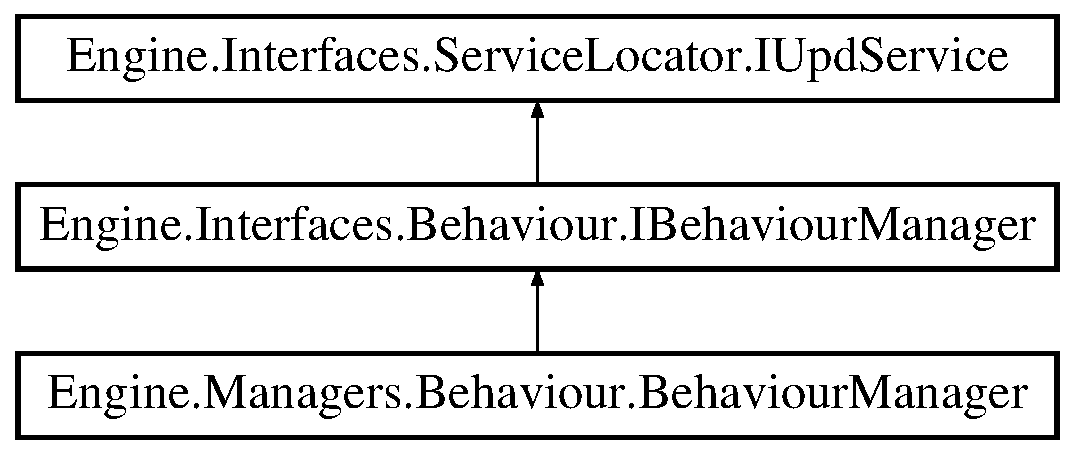
\includegraphics[height=3.000000cm]{de/df7/a00418}
\end{center}
\end{figure}
\subsection*{Public Member Functions}
\begin{DoxyCompactItemize}
\item 
\hyperlink{a00446}{I\+Mind} \hyperlink{a00418_ad821620edeb0239197446bf1c3c32ee3}{Create$<$ T $>$} (\hyperlink{a00438}{I\+Entity} ie)
\begin{DoxyCompactList}\small\item\em M\+E\+T\+H\+OD\+: Create a new I\+Mind of type T \end{DoxyCompactList}\item 
void \hyperlink{a00418_ae944227a75ab665c4140628279296580}{clear\+List} ()
\begin{DoxyCompactList}\small\item\em M\+E\+T\+H\+OD\+: Clears the current list of all minds \end{DoxyCompactList}\item 
void \hyperlink{a00418_a6f89adf3a1d8286a73b534855847c414}{remove\+Mind} (int id)
\begin{DoxyCompactList}\small\item\em M\+E\+T\+H\+OD\+: Removes a specific mind from the list based on the id provided \end{DoxyCompactList}\item 
\hyperlink{a00446}{I\+Mind} \hyperlink{a00418_ac1d24fb690a665ce8c70671b7c27b9ad}{get\+Mind} (int id)
\begin{DoxyCompactList}\small\item\em M\+E\+T\+H\+OD\+: Returns a mind based on the unique ID provided \end{DoxyCompactList}\item 
void \hyperlink{a00418_af161090c055167e2ca3901ed13d3d128}{Update} (Game\+Time game\+Time)
\begin{DoxyCompactList}\small\item\em M\+E\+T\+H\+OD\+: The update loop which is cycled through ever frame \end{DoxyCompactList}\end{DoxyCompactItemize}


\subsection{Member Function Documentation}
\mbox{\Hypertarget{a00418_ae944227a75ab665c4140628279296580}\label{a00418_ae944227a75ab665c4140628279296580}} 
\index{Engine\+::\+Interfaces\+::\+Behaviour\+::\+I\+Behaviour\+Manager@{Engine\+::\+Interfaces\+::\+Behaviour\+::\+I\+Behaviour\+Manager}!clear\+List@{clear\+List}}
\index{clear\+List@{clear\+List}!Engine\+::\+Interfaces\+::\+Behaviour\+::\+I\+Behaviour\+Manager@{Engine\+::\+Interfaces\+::\+Behaviour\+::\+I\+Behaviour\+Manager}}
\subsubsection{\texorpdfstring{clear\+List()}{clearList()}}
{\footnotesize\ttfamily void Engine.\+Interfaces.\+Behaviour.\+I\+Behaviour\+Manager.\+clear\+List (\begin{DoxyParamCaption}{ }\end{DoxyParamCaption})}



M\+E\+T\+H\+OD\+: Clears the current list of all minds 



Implemented in \hyperlink{a00486_ae21fe19ea423236e26d4f022230a071e}{Engine.\+Managers.\+Behaviour.\+Behaviour\+Manager}.

\mbox{\Hypertarget{a00418_ad821620edeb0239197446bf1c3c32ee3}\label{a00418_ad821620edeb0239197446bf1c3c32ee3}} 
\index{Engine\+::\+Interfaces\+::\+Behaviour\+::\+I\+Behaviour\+Manager@{Engine\+::\+Interfaces\+::\+Behaviour\+::\+I\+Behaviour\+Manager}!Create$<$ T $>$@{Create$<$ T $>$}}
\index{Create$<$ T $>$@{Create$<$ T $>$}!Engine\+::\+Interfaces\+::\+Behaviour\+::\+I\+Behaviour\+Manager@{Engine\+::\+Interfaces\+::\+Behaviour\+::\+I\+Behaviour\+Manager}}
\subsubsection{\texorpdfstring{Create$<$ T $>$()}{Create< T >()}}
{\footnotesize\ttfamily \hyperlink{a00446}{I\+Mind} Engine.\+Interfaces.\+Behaviour.\+I\+Behaviour\+Manager.\+Create$<$ T $>$ (\begin{DoxyParamCaption}\item[{\hyperlink{a00438}{I\+Entity}}]{ie }\end{DoxyParamCaption})}



M\+E\+T\+H\+OD\+: Create a new I\+Mind of type T 


\begin{DoxyTemplParams}{Template Parameters}
{\em T} & Generic type for the mind that will be created\\
\hline
\end{DoxyTemplParams}

\begin{DoxyParams}{Parameters}
{\em ie} & the Entity the mind will be linked to\\
\hline
\end{DoxyParams}
\begin{DoxyReturn}{Returns}
a brand new I\+Mind
\end{DoxyReturn}


Implemented in \hyperlink{a00486_a13eea511ff6d2cdeb8287b63034ce898}{Engine.\+Managers.\+Behaviour.\+Behaviour\+Manager}.

\begin{Desc}
\item[Type Constraints]\begin{description}
\item[{\em T} : {\em I\+Mind}]\item[{\em T} : {\em new()}]\end{description}
\end{Desc}
\mbox{\Hypertarget{a00418_ac1d24fb690a665ce8c70671b7c27b9ad}\label{a00418_ac1d24fb690a665ce8c70671b7c27b9ad}} 
\index{Engine\+::\+Interfaces\+::\+Behaviour\+::\+I\+Behaviour\+Manager@{Engine\+::\+Interfaces\+::\+Behaviour\+::\+I\+Behaviour\+Manager}!get\+Mind@{get\+Mind}}
\index{get\+Mind@{get\+Mind}!Engine\+::\+Interfaces\+::\+Behaviour\+::\+I\+Behaviour\+Manager@{Engine\+::\+Interfaces\+::\+Behaviour\+::\+I\+Behaviour\+Manager}}
\subsubsection{\texorpdfstring{get\+Mind()}{getMind()}}
{\footnotesize\ttfamily \hyperlink{a00446}{I\+Mind} Engine.\+Interfaces.\+Behaviour.\+I\+Behaviour\+Manager.\+get\+Mind (\begin{DoxyParamCaption}\item[{int}]{id }\end{DoxyParamCaption})}



M\+E\+T\+H\+OD\+: Returns a mind based on the unique ID provided 


\begin{DoxyParams}{Parameters}
{\em id} & the Unique ID of the mind to be returned\\
\hline
\end{DoxyParams}
\begin{DoxyReturn}{Returns}
the I\+Mind associated with the id
\end{DoxyReturn}


Implemented in \hyperlink{a00486_a4391a84eadd13a812977cd51e177e00b}{Engine.\+Managers.\+Behaviour.\+Behaviour\+Manager}.

\mbox{\Hypertarget{a00418_a6f89adf3a1d8286a73b534855847c414}\label{a00418_a6f89adf3a1d8286a73b534855847c414}} 
\index{Engine\+::\+Interfaces\+::\+Behaviour\+::\+I\+Behaviour\+Manager@{Engine\+::\+Interfaces\+::\+Behaviour\+::\+I\+Behaviour\+Manager}!remove\+Mind@{remove\+Mind}}
\index{remove\+Mind@{remove\+Mind}!Engine\+::\+Interfaces\+::\+Behaviour\+::\+I\+Behaviour\+Manager@{Engine\+::\+Interfaces\+::\+Behaviour\+::\+I\+Behaviour\+Manager}}
\subsubsection{\texorpdfstring{remove\+Mind()}{removeMind()}}
{\footnotesize\ttfamily void Engine.\+Interfaces.\+Behaviour.\+I\+Behaviour\+Manager.\+remove\+Mind (\begin{DoxyParamCaption}\item[{int}]{id }\end{DoxyParamCaption})}



M\+E\+T\+H\+OD\+: Removes a specific mind from the list based on the id provided 


\begin{DoxyParams}{Parameters}
{\em id} & the unique ID of the mind to be removed\\
\hline
\end{DoxyParams}


Implemented in \hyperlink{a00486_a684853fb49121d19f4d5c635153b871a}{Engine.\+Managers.\+Behaviour.\+Behaviour\+Manager}.

\mbox{\Hypertarget{a00418_af161090c055167e2ca3901ed13d3d128}\label{a00418_af161090c055167e2ca3901ed13d3d128}} 
\index{Engine\+::\+Interfaces\+::\+Behaviour\+::\+I\+Behaviour\+Manager@{Engine\+::\+Interfaces\+::\+Behaviour\+::\+I\+Behaviour\+Manager}!Update@{Update}}
\index{Update@{Update}!Engine\+::\+Interfaces\+::\+Behaviour\+::\+I\+Behaviour\+Manager@{Engine\+::\+Interfaces\+::\+Behaviour\+::\+I\+Behaviour\+Manager}}
\subsubsection{\texorpdfstring{Update()}{Update()}}
{\footnotesize\ttfamily void Engine.\+Interfaces.\+Behaviour.\+I\+Behaviour\+Manager.\+Update (\begin{DoxyParamCaption}\item[{Game\+Time}]{game\+Time }\end{DoxyParamCaption})}



M\+E\+T\+H\+OD\+: The update loop which is cycled through ever frame 


\begin{DoxyParams}{Parameters}
{\em game\+Time} & The Mono\+Game Gametime property\\
\hline
\end{DoxyParams}


Implements \hyperlink{a00478_a387fce2a5440a4dc63f8d72772ecbdaa}{Engine.\+Interfaces.\+Service\+Locator.\+I\+Upd\+Service}.



Implemented in \hyperlink{a00486_a729bf10d2469de0497d75dfadbf56506}{Engine.\+Managers.\+Behaviour.\+Behaviour\+Manager}.



The documentation for this interface was generated from the following file\+:\begin{DoxyCompactItemize}
\item 
\hyperlink{a00095}{I\+Behaviour\+Manager.\+cs}\end{DoxyCompactItemize}

\hypertarget{a00422}{}\section{Engine.\+Interfaces.\+Cam.\+I\+Camera\+Manager Interface Reference}
\label{a00422}\index{Engine.\+Interfaces.\+Cam.\+I\+Camera\+Manager@{Engine.\+Interfaces.\+Cam.\+I\+Camera\+Manager}}


I\+N\+T\+E\+R\+F\+A\+CE\+:The interface for the Camera manager. This controls the implementation for the manager of the camera.  


Inheritance diagram for Engine.\+Interfaces.\+Cam.\+I\+Camera\+Manager\+:\begin{figure}[H]
\begin{center}
\leavevmode
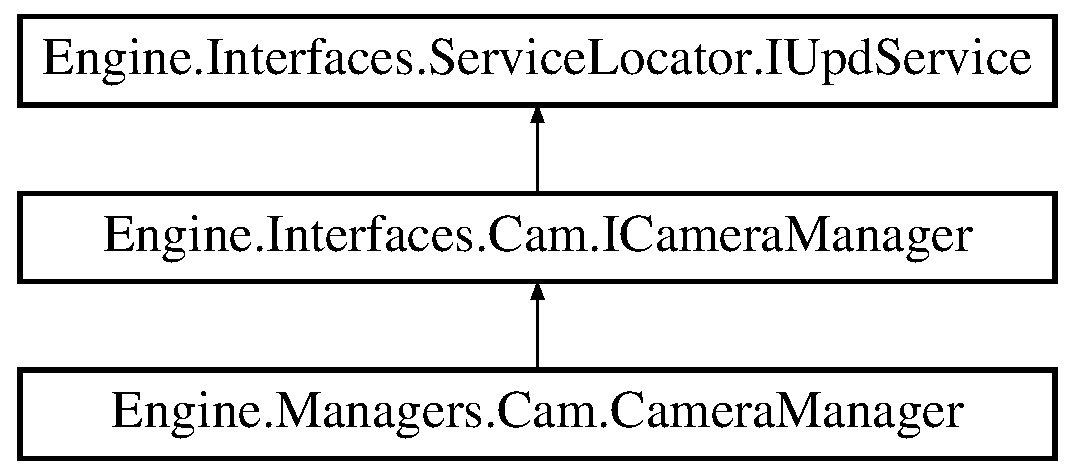
\includegraphics[height=3.000000cm]{db/d43/a00422}
\end{center}
\end{figure}
\subsection*{Public Member Functions}
\begin{DoxyCompactItemize}
\item 
void \hyperlink{a00422_a21e0ce6b0ada068546161ecf02559912}{Initialize} ()
\begin{DoxyCompactList}\small\item\em M\+E\+T\+H\+OD\+: Contains initialisation logic \end{DoxyCompactList}\item 
\hyperlink{a00490}{Camera} \hyperlink{a00422_a91fc1dab51b36fd8955451ac00fd2819}{get\+Cam} ()
\begin{DoxyCompactList}\small\item\em M\+E\+T\+H\+OD\+: Returns the camera \end{DoxyCompactList}\item 
void \hyperlink{a00422_a78a46559249e70181100daff38ef5d6a}{Update} (Game\+Time game\+Time)
\begin{DoxyCompactList}\small\item\em M\+E\+T\+H\+OD\+: The update loop which is cycled through every frame \end{DoxyCompactList}\item 
Vector2 \hyperlink{a00422_a7d9fc1d792ddc3495bff23daac2a8d2a}{get\+World\+Position} (Vector2 Position)
\begin{DoxyCompactList}\small\item\em M\+E\+T\+H\+OD\+: returns the current world position in relation to the Vector2 provided \end{DoxyCompactList}\end{DoxyCompactItemize}


\subsection{Detailed Description}
I\+N\+T\+E\+R\+F\+A\+CE\+:The interface for the Camera manager. This controls the implementation for the manager of the camera. 



\subsection{Member Function Documentation}
\mbox{\Hypertarget{a00422_a91fc1dab51b36fd8955451ac00fd2819}\label{a00422_a91fc1dab51b36fd8955451ac00fd2819}} 
\index{Engine\+::\+Interfaces\+::\+Cam\+::\+I\+Camera\+Manager@{Engine\+::\+Interfaces\+::\+Cam\+::\+I\+Camera\+Manager}!get\+Cam@{get\+Cam}}
\index{get\+Cam@{get\+Cam}!Engine\+::\+Interfaces\+::\+Cam\+::\+I\+Camera\+Manager@{Engine\+::\+Interfaces\+::\+Cam\+::\+I\+Camera\+Manager}}
\subsubsection{\texorpdfstring{get\+Cam()}{getCam()}}
{\footnotesize\ttfamily \hyperlink{a00490}{Camera} Engine.\+Interfaces.\+Cam.\+I\+Camera\+Manager.\+get\+Cam (\begin{DoxyParamCaption}{ }\end{DoxyParamCaption})}



M\+E\+T\+H\+OD\+: Returns the camera 

\begin{DoxyReturn}{Returns}
the current Camera
\end{DoxyReturn}


Implemented in \hyperlink{a00494_a949b09e5c57971945c3ccb638f73765d}{Engine.\+Managers.\+Cam.\+Camera\+Manager}.

\mbox{\Hypertarget{a00422_a7d9fc1d792ddc3495bff23daac2a8d2a}\label{a00422_a7d9fc1d792ddc3495bff23daac2a8d2a}} 
\index{Engine\+::\+Interfaces\+::\+Cam\+::\+I\+Camera\+Manager@{Engine\+::\+Interfaces\+::\+Cam\+::\+I\+Camera\+Manager}!get\+World\+Position@{get\+World\+Position}}
\index{get\+World\+Position@{get\+World\+Position}!Engine\+::\+Interfaces\+::\+Cam\+::\+I\+Camera\+Manager@{Engine\+::\+Interfaces\+::\+Cam\+::\+I\+Camera\+Manager}}
\subsubsection{\texorpdfstring{get\+World\+Position()}{getWorldPosition()}}
{\footnotesize\ttfamily Vector2 Engine.\+Interfaces.\+Cam.\+I\+Camera\+Manager.\+get\+World\+Position (\begin{DoxyParamCaption}\item[{Vector2}]{Position }\end{DoxyParamCaption})}



M\+E\+T\+H\+OD\+: returns the current world position in relation to the Vector2 provided 


\begin{DoxyParams}{Parameters}
{\em Position} & The position to be compared to the world position\\
\hline
\end{DoxyParams}
\begin{DoxyReturn}{Returns}
The world position in relation to the Vector2 provided
\end{DoxyReturn}


Implemented in \hyperlink{a00494_a538af3b5745f1f51e3da217d5c971791}{Engine.\+Managers.\+Cam.\+Camera\+Manager}.

\mbox{\Hypertarget{a00422_a21e0ce6b0ada068546161ecf02559912}\label{a00422_a21e0ce6b0ada068546161ecf02559912}} 
\index{Engine\+::\+Interfaces\+::\+Cam\+::\+I\+Camera\+Manager@{Engine\+::\+Interfaces\+::\+Cam\+::\+I\+Camera\+Manager}!Initialize@{Initialize}}
\index{Initialize@{Initialize}!Engine\+::\+Interfaces\+::\+Cam\+::\+I\+Camera\+Manager@{Engine\+::\+Interfaces\+::\+Cam\+::\+I\+Camera\+Manager}}
\subsubsection{\texorpdfstring{Initialize()}{Initialize()}}
{\footnotesize\ttfamily void Engine.\+Interfaces.\+Cam.\+I\+Camera\+Manager.\+Initialize (\begin{DoxyParamCaption}{ }\end{DoxyParamCaption})}



M\+E\+T\+H\+OD\+: Contains initialisation logic 



Implemented in \hyperlink{a00494_a6244a0582982e64f49df0a6862768a21}{Engine.\+Managers.\+Cam.\+Camera\+Manager}.

\mbox{\Hypertarget{a00422_a78a46559249e70181100daff38ef5d6a}\label{a00422_a78a46559249e70181100daff38ef5d6a}} 
\index{Engine\+::\+Interfaces\+::\+Cam\+::\+I\+Camera\+Manager@{Engine\+::\+Interfaces\+::\+Cam\+::\+I\+Camera\+Manager}!Update@{Update}}
\index{Update@{Update}!Engine\+::\+Interfaces\+::\+Cam\+::\+I\+Camera\+Manager@{Engine\+::\+Interfaces\+::\+Cam\+::\+I\+Camera\+Manager}}
\subsubsection{\texorpdfstring{Update()}{Update()}}
{\footnotesize\ttfamily void Engine.\+Interfaces.\+Cam.\+I\+Camera\+Manager.\+Update (\begin{DoxyParamCaption}\item[{Game\+Time}]{game\+Time }\end{DoxyParamCaption})}



M\+E\+T\+H\+OD\+: The update loop which is cycled through every frame 


\begin{DoxyParams}{Parameters}
{\em game\+Time} & \\
\hline
\end{DoxyParams}


Implements \hyperlink{a00478_a387fce2a5440a4dc63f8d72772ecbdaa}{Engine.\+Interfaces.\+Service\+Locator.\+I\+Upd\+Service}.



Implemented in \hyperlink{a00494_a43e367859b47354445da2a304eff7ec4}{Engine.\+Managers.\+Cam.\+Camera\+Manager}.



The documentation for this interface was generated from the following file\+:\begin{DoxyCompactItemize}
\item 
\hyperlink{a00098}{I\+Camera\+Manager.\+cs}\end{DoxyCompactItemize}

\hypertarget{a00426}{}\section{Engine.\+Interfaces.\+Collision.\+I\+Collidable Interface Reference}
\label{a00426}\index{Engine.\+Interfaces.\+Collision.\+I\+Collidable@{Engine.\+Interfaces.\+Collision.\+I\+Collidable}}


I\+N\+T\+E\+R\+F\+A\+CE\+: An interface used for objects that will need collision calculation during the game loop  


Inheritance diagram for Engine.\+Interfaces.\+Collision.\+I\+Collidable\+:\begin{figure}[H]
\begin{center}
\leavevmode
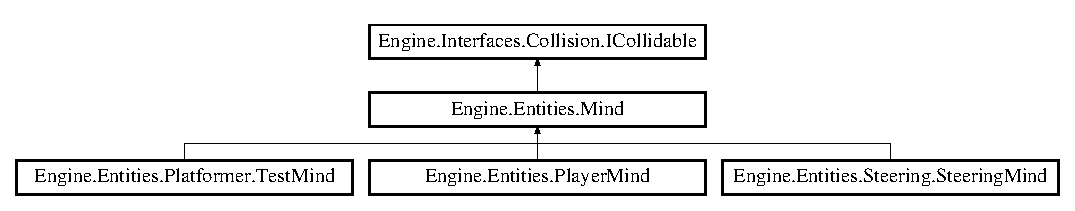
\includegraphics[height=2.393162cm]{d7/db9/a00426}
\end{center}
\end{figure}
\subsection*{Public Member Functions}
\begin{DoxyCompactItemize}
\item 
void \hyperlink{a00426_a000ca0336b06e3f2d658d442a83dbbbb}{Apply\+Impulse} (Vector2 c\+Velocity)
\begin{DoxyCompactList}\small\item\em Apply\+Impulse is the response from collision. After the object has been moved by the minimum translation vector It will have a reactionary force applied to it in order to simulate physics. \end{DoxyCompactList}\end{DoxyCompactItemize}
\subsection*{Properties}
\begin{DoxyCompactItemize}
\item 
Rectangle \hyperlink{a00426_aa4cbc57adf743bacff53f85bb4a2fcf3}{Bounds}\hspace{0.3cm}{\ttfamily  \mbox{[}get\mbox{]}}
\begin{DoxyCompactList}\small\item\em G\+ET\+: The axis aligned bounds of the object. \end{DoxyCompactList}\item 
Vector2 \hyperlink{a00426_a4e17a9b41927fab6d2973c4feb0a993a}{Position}\hspace{0.3cm}{\ttfamily  \mbox{[}get, set\mbox{]}}
\begin{DoxyCompactList}\small\item\em G\+ET\+: S\+ET\+: The position of the object. \end{DoxyCompactList}\item 
bool \hyperlink{a00426_a833b30a82fe2f6ae78ea7b84fe742b35}{is\+Collidable}\hspace{0.3cm}{\ttfamily  \mbox{[}get, set\mbox{]}}
\begin{DoxyCompactList}\small\item\em G\+TE\+: S\+ET\+: A boolean to tell whether an object is to be tested for collision or not. \end{DoxyCompactList}\item 
bool \hyperlink{a00426_a04dfebf647bfd0967be3dd4ba76706e5}{is\+Colliding}\hspace{0.3cm}{\ttfamily  \mbox{[}get, set\mbox{]}}
\begin{DoxyCompactList}\small\item\em G\+ET\+: S\+ET\+: A boolean to tell whether an object is currently colliding or not. \end{DoxyCompactList}\item 
List$<$ \hyperlink{a00434}{I\+Hitbox} $>$ \hyperlink{a00426_a0a723609d175ef0f7eca7002572a76bb}{Hits}\hspace{0.3cm}{\ttfamily  \mbox{[}get, set\mbox{]}}
\begin{DoxyCompactList}\small\item\em A list of hitboxes used for calculating collision. \end{DoxyCompactList}\end{DoxyCompactItemize}


\subsection{Detailed Description}
I\+N\+T\+E\+R\+F\+A\+CE\+: An interface used for objects that will need collision calculation during the game loop 



\subsection{Member Function Documentation}
\mbox{\Hypertarget{a00426_a000ca0336b06e3f2d658d442a83dbbbb}\label{a00426_a000ca0336b06e3f2d658d442a83dbbbb}} 
\index{Engine\+::\+Interfaces\+::\+Collision\+::\+I\+Collidable@{Engine\+::\+Interfaces\+::\+Collision\+::\+I\+Collidable}!Apply\+Impulse@{Apply\+Impulse}}
\index{Apply\+Impulse@{Apply\+Impulse}!Engine\+::\+Interfaces\+::\+Collision\+::\+I\+Collidable@{Engine\+::\+Interfaces\+::\+Collision\+::\+I\+Collidable}}
\subsubsection{\texorpdfstring{Apply\+Impulse()}{ApplyImpulse()}}
{\footnotesize\ttfamily void Engine.\+Interfaces.\+Collision.\+I\+Collidable.\+Apply\+Impulse (\begin{DoxyParamCaption}\item[{Vector2}]{c\+Velocity }\end{DoxyParamCaption})}



Apply\+Impulse is the response from collision. After the object has been moved by the minimum translation vector It will have a reactionary force applied to it in order to simulate physics. 


\begin{DoxyParams}{Parameters}
{\em c\+Velocity} & \\
\hline
\end{DoxyParams}


Implemented in \hyperlink{a00318_a378218df0a8c27a981e98167197d9c16}{Engine.\+Entities.\+Mind}.



\subsection{Property Documentation}
\mbox{\Hypertarget{a00426_aa4cbc57adf743bacff53f85bb4a2fcf3}\label{a00426_aa4cbc57adf743bacff53f85bb4a2fcf3}} 
\index{Engine\+::\+Interfaces\+::\+Collision\+::\+I\+Collidable@{Engine\+::\+Interfaces\+::\+Collision\+::\+I\+Collidable}!Bounds@{Bounds}}
\index{Bounds@{Bounds}!Engine\+::\+Interfaces\+::\+Collision\+::\+I\+Collidable@{Engine\+::\+Interfaces\+::\+Collision\+::\+I\+Collidable}}
\subsubsection{\texorpdfstring{Bounds}{Bounds}}
{\footnotesize\ttfamily Rectangle Engine.\+Interfaces.\+Collision.\+I\+Collidable.\+Bounds\hspace{0.3cm}{\ttfamily [get]}}



G\+ET\+: The axis aligned bounds of the object. 

\mbox{\Hypertarget{a00426_a0a723609d175ef0f7eca7002572a76bb}\label{a00426_a0a723609d175ef0f7eca7002572a76bb}} 
\index{Engine\+::\+Interfaces\+::\+Collision\+::\+I\+Collidable@{Engine\+::\+Interfaces\+::\+Collision\+::\+I\+Collidable}!Hits@{Hits}}
\index{Hits@{Hits}!Engine\+::\+Interfaces\+::\+Collision\+::\+I\+Collidable@{Engine\+::\+Interfaces\+::\+Collision\+::\+I\+Collidable}}
\subsubsection{\texorpdfstring{Hits}{Hits}}
{\footnotesize\ttfamily List$<$\hyperlink{a00434}{I\+Hitbox}$>$ Engine.\+Interfaces.\+Collision.\+I\+Collidable.\+Hits\hspace{0.3cm}{\ttfamily [get]}, {\ttfamily [set]}}



A list of hitboxes used for calculating collision. 

\mbox{\Hypertarget{a00426_a833b30a82fe2f6ae78ea7b84fe742b35}\label{a00426_a833b30a82fe2f6ae78ea7b84fe742b35}} 
\index{Engine\+::\+Interfaces\+::\+Collision\+::\+I\+Collidable@{Engine\+::\+Interfaces\+::\+Collision\+::\+I\+Collidable}!is\+Collidable@{is\+Collidable}}
\index{is\+Collidable@{is\+Collidable}!Engine\+::\+Interfaces\+::\+Collision\+::\+I\+Collidable@{Engine\+::\+Interfaces\+::\+Collision\+::\+I\+Collidable}}
\subsubsection{\texorpdfstring{is\+Collidable}{isCollidable}}
{\footnotesize\ttfamily bool Engine.\+Interfaces.\+Collision.\+I\+Collidable.\+is\+Collidable\hspace{0.3cm}{\ttfamily [get]}, {\ttfamily [set]}}



G\+TE\+: S\+ET\+: A boolean to tell whether an object is to be tested for collision or not. 

\mbox{\Hypertarget{a00426_a04dfebf647bfd0967be3dd4ba76706e5}\label{a00426_a04dfebf647bfd0967be3dd4ba76706e5}} 
\index{Engine\+::\+Interfaces\+::\+Collision\+::\+I\+Collidable@{Engine\+::\+Interfaces\+::\+Collision\+::\+I\+Collidable}!is\+Colliding@{is\+Colliding}}
\index{is\+Colliding@{is\+Colliding}!Engine\+::\+Interfaces\+::\+Collision\+::\+I\+Collidable@{Engine\+::\+Interfaces\+::\+Collision\+::\+I\+Collidable}}
\subsubsection{\texorpdfstring{is\+Colliding}{isColliding}}
{\footnotesize\ttfamily bool Engine.\+Interfaces.\+Collision.\+I\+Collidable.\+is\+Colliding\hspace{0.3cm}{\ttfamily [get]}, {\ttfamily [set]}}



G\+ET\+: S\+ET\+: A boolean to tell whether an object is currently colliding or not. 

\mbox{\Hypertarget{a00426_a4e17a9b41927fab6d2973c4feb0a993a}\label{a00426_a4e17a9b41927fab6d2973c4feb0a993a}} 
\index{Engine\+::\+Interfaces\+::\+Collision\+::\+I\+Collidable@{Engine\+::\+Interfaces\+::\+Collision\+::\+I\+Collidable}!Position@{Position}}
\index{Position@{Position}!Engine\+::\+Interfaces\+::\+Collision\+::\+I\+Collidable@{Engine\+::\+Interfaces\+::\+Collision\+::\+I\+Collidable}}
\subsubsection{\texorpdfstring{Position}{Position}}
{\footnotesize\ttfamily Vector2 Engine.\+Interfaces.\+Collision.\+I\+Collidable.\+Position\hspace{0.3cm}{\ttfamily [get]}, {\ttfamily [set]}}



G\+ET\+: S\+ET\+: The position of the object. 



The documentation for this interface was generated from the following file\+:\begin{DoxyCompactItemize}
\item 
\hyperlink{a00101}{I\+Collidable.\+cs}\end{DoxyCompactItemize}

\hypertarget{a00430}{}\section{Engine.\+Interfaces.\+Collision.\+I\+Detection\+Manager Interface Reference}
\label{a00430}\index{Engine.\+Interfaces.\+Collision.\+I\+Detection\+Manager@{Engine.\+Interfaces.\+Collision.\+I\+Detection\+Manager}}


I\+N\+T\+E\+R\+F\+A\+CE\+: An interface for the collision detection manager  


Inheritance diagram for Engine.\+Interfaces.\+Collision.\+I\+Detection\+Manager\+:\begin{figure}[H]
\begin{center}
\leavevmode
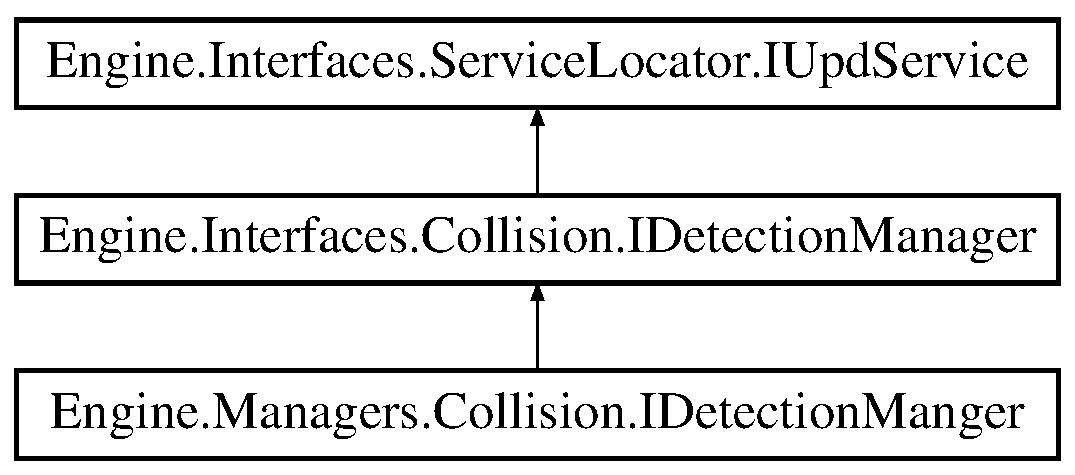
\includegraphics[height=3.000000cm]{dc/d0c/a00430}
\end{center}
\end{figure}
\subsection*{Public Member Functions}
\begin{DoxyCompactItemize}
\item 
void \hyperlink{a00430_a11808ec009ee682fa73e3c4ea6570139}{add\+Collidable} (\hyperlink{a00426}{I\+Collidable} obj)
\begin{DoxyCompactList}\small\item\em M\+E\+T\+H\+OD\+: Adds an I\+C\+Ollidable to the list of objects to check \end{DoxyCompactList}\item 
void \hyperlink{a00430_aeaa36b46e3ecd301b2fce9197fb0a35c}{Update} (Game\+Time game\+Time)
\begin{DoxyCompactList}\small\item\em M\+E\+T\+H\+OD\+: The update loop which is cycled through every frame \end{DoxyCompactList}\item 
void \hyperlink{a00430_a139cca7ebb8b37ceba1bb1439cde83bf}{do\+Collision} ()
\begin{DoxyCompactList}\small\item\em M\+E\+T\+H\+OD\+: Checks A\+A\+BB \hyperlink{a00255}{Collision} for two objects \end{DoxyCompactList}\item 
void \hyperlink{a00430_ac0f8278b5b5a1c103da46f154ad088dc}{On\+A\+Collision} (\hyperlink{a00426}{I\+Collidable} A, \hyperlink{a00426}{I\+Collidable} B)
\begin{DoxyCompactList}\small\item\em M\+E\+T\+H\+OD\+: When two objects are colliding via A\+A\+BB collision, this method is called \end{DoxyCompactList}\item 
void \hyperlink{a00430_ad87743faa9c3c212879716d7306c4fb3}{Call\+S\+AT} (\hyperlink{a00426}{I\+Collidable} A, \hyperlink{a00426}{I\+Collidable} B, Vector2 mtv)
\begin{DoxyCompactList}\small\item\em M\+E\+T\+H\+OD\+: When two objects are calculated to be colliding with the S\+AT logic, this method is called and moves them apart \end{DoxyCompactList}\item 
void \hyperlink{a00430_a1acd238daa104a8f4dcf36536e1ac9f9}{Check\+S\+AT} (\hyperlink{a00426}{I\+Collidable} a, \hyperlink{a00426}{I\+Collidable} b)
\begin{DoxyCompactList}\small\item\em M\+E\+T\+H\+OD\+: Checks for whether or not two objects are colliding according to the S\+AT Logic \end{DoxyCompactList}\item 
Vector2 \hyperlink{a00430_a853912077b127d7e6779accc914df3cf}{Impulse\+Application} (\hyperlink{a00434}{I\+Hitbox} a, \hyperlink{a00434}{I\+Hitbox} b)
\begin{DoxyCompactList}\small\item\em M\+E\+T\+H\+OD\+: Creates the impulse to be applied to an entity when it is colliding allowing it to simulate physics when it reacts \end{DoxyCompactList}\end{DoxyCompactItemize}


\subsection{Detailed Description}
I\+N\+T\+E\+R\+F\+A\+CE\+: An interface for the collision detection manager 



\subsection{Member Function Documentation}
\mbox{\Hypertarget{a00430_a11808ec009ee682fa73e3c4ea6570139}\label{a00430_a11808ec009ee682fa73e3c4ea6570139}} 
\index{Engine\+::\+Interfaces\+::\+Collision\+::\+I\+Detection\+Manager@{Engine\+::\+Interfaces\+::\+Collision\+::\+I\+Detection\+Manager}!add\+Collidable@{add\+Collidable}}
\index{add\+Collidable@{add\+Collidable}!Engine\+::\+Interfaces\+::\+Collision\+::\+I\+Detection\+Manager@{Engine\+::\+Interfaces\+::\+Collision\+::\+I\+Detection\+Manager}}
\subsubsection{\texorpdfstring{add\+Collidable()}{addCollidable()}}
{\footnotesize\ttfamily void Engine.\+Interfaces.\+Collision.\+I\+Detection\+Manager.\+add\+Collidable (\begin{DoxyParamCaption}\item[{\hyperlink{a00426}{I\+Collidable}}]{obj }\end{DoxyParamCaption})}



M\+E\+T\+H\+OD\+: Adds an I\+C\+Ollidable to the list of objects to check 


\begin{DoxyParams}{Parameters}
{\em obj} & The object to add to the list\\
\hline
\end{DoxyParams}


Implemented in \hyperlink{a00502_ae4daf9d957c8b30e779a7ed89237b370}{Engine.\+Managers.\+Collision.\+I\+Detection\+Manger}.

\mbox{\Hypertarget{a00430_ad87743faa9c3c212879716d7306c4fb3}\label{a00430_ad87743faa9c3c212879716d7306c4fb3}} 
\index{Engine\+::\+Interfaces\+::\+Collision\+::\+I\+Detection\+Manager@{Engine\+::\+Interfaces\+::\+Collision\+::\+I\+Detection\+Manager}!Call\+S\+AT@{Call\+S\+AT}}
\index{Call\+S\+AT@{Call\+S\+AT}!Engine\+::\+Interfaces\+::\+Collision\+::\+I\+Detection\+Manager@{Engine\+::\+Interfaces\+::\+Collision\+::\+I\+Detection\+Manager}}
\subsubsection{\texorpdfstring{Call\+S\+A\+T()}{CallSAT()}}
{\footnotesize\ttfamily void Engine.\+Interfaces.\+Collision.\+I\+Detection\+Manager.\+Call\+S\+AT (\begin{DoxyParamCaption}\item[{\hyperlink{a00426}{I\+Collidable}}]{A,  }\item[{\hyperlink{a00426}{I\+Collidable}}]{B,  }\item[{Vector2}]{mtv }\end{DoxyParamCaption})}



M\+E\+T\+H\+OD\+: When two objects are calculated to be colliding with the S\+AT logic, this method is called and moves them apart 


\begin{DoxyParams}{Parameters}
{\em A} & The first object that\textquotesingle{}s colliding\\
\hline
{\em B} & The second object that\textquotesingle{}s colliding\\
\hline
{\em mtv} & The minimum translation vector calculated in the S\+AT Loop\\
\hline
\end{DoxyParams}


Implemented in \hyperlink{a00502_a272b97e8ab5caf3dcceb455849deb6ed}{Engine.\+Managers.\+Collision.\+I\+Detection\+Manger}.

\mbox{\Hypertarget{a00430_a1acd238daa104a8f4dcf36536e1ac9f9}\label{a00430_a1acd238daa104a8f4dcf36536e1ac9f9}} 
\index{Engine\+::\+Interfaces\+::\+Collision\+::\+I\+Detection\+Manager@{Engine\+::\+Interfaces\+::\+Collision\+::\+I\+Detection\+Manager}!Check\+S\+AT@{Check\+S\+AT}}
\index{Check\+S\+AT@{Check\+S\+AT}!Engine\+::\+Interfaces\+::\+Collision\+::\+I\+Detection\+Manager@{Engine\+::\+Interfaces\+::\+Collision\+::\+I\+Detection\+Manager}}
\subsubsection{\texorpdfstring{Check\+S\+A\+T()}{CheckSAT()}}
{\footnotesize\ttfamily void Engine.\+Interfaces.\+Collision.\+I\+Detection\+Manager.\+Check\+S\+AT (\begin{DoxyParamCaption}\item[{\hyperlink{a00426}{I\+Collidable}}]{a,  }\item[{\hyperlink{a00426}{I\+Collidable}}]{b }\end{DoxyParamCaption})}



M\+E\+T\+H\+OD\+: Checks for whether or not two objects are colliding according to the S\+AT Logic 


\begin{DoxyParams}{Parameters}
{\em a} & The first object that\textquotesingle{}s colliding\\
\hline
{\em b} & The second object that\textquotesingle{}s colliding\\
\hline
\end{DoxyParams}


Implemented in \hyperlink{a00502_a18f0056903776f291a462fb4bbbfc224}{Engine.\+Managers.\+Collision.\+I\+Detection\+Manger}.

\mbox{\Hypertarget{a00430_a139cca7ebb8b37ceba1bb1439cde83bf}\label{a00430_a139cca7ebb8b37ceba1bb1439cde83bf}} 
\index{Engine\+::\+Interfaces\+::\+Collision\+::\+I\+Detection\+Manager@{Engine\+::\+Interfaces\+::\+Collision\+::\+I\+Detection\+Manager}!do\+Collision@{do\+Collision}}
\index{do\+Collision@{do\+Collision}!Engine\+::\+Interfaces\+::\+Collision\+::\+I\+Detection\+Manager@{Engine\+::\+Interfaces\+::\+Collision\+::\+I\+Detection\+Manager}}
\subsubsection{\texorpdfstring{do\+Collision()}{doCollision()}}
{\footnotesize\ttfamily void Engine.\+Interfaces.\+Collision.\+I\+Detection\+Manager.\+do\+Collision (\begin{DoxyParamCaption}{ }\end{DoxyParamCaption})}



M\+E\+T\+H\+OD\+: Checks A\+A\+BB \hyperlink{a00255}{Collision} for two objects 



Implemented in \hyperlink{a00502_a6785a08302cfe7d6fb08a7042691a3a8}{Engine.\+Managers.\+Collision.\+I\+Detection\+Manger}.

\mbox{\Hypertarget{a00430_a853912077b127d7e6779accc914df3cf}\label{a00430_a853912077b127d7e6779accc914df3cf}} 
\index{Engine\+::\+Interfaces\+::\+Collision\+::\+I\+Detection\+Manager@{Engine\+::\+Interfaces\+::\+Collision\+::\+I\+Detection\+Manager}!Impulse\+Application@{Impulse\+Application}}
\index{Impulse\+Application@{Impulse\+Application}!Engine\+::\+Interfaces\+::\+Collision\+::\+I\+Detection\+Manager@{Engine\+::\+Interfaces\+::\+Collision\+::\+I\+Detection\+Manager}}
\subsubsection{\texorpdfstring{Impulse\+Application()}{ImpulseApplication()}}
{\footnotesize\ttfamily Vector2 Engine.\+Interfaces.\+Collision.\+I\+Detection\+Manager.\+Impulse\+Application (\begin{DoxyParamCaption}\item[{\hyperlink{a00434}{I\+Hitbox}}]{a,  }\item[{\hyperlink{a00434}{I\+Hitbox}}]{b }\end{DoxyParamCaption})}



M\+E\+T\+H\+OD\+: Creates the impulse to be applied to an entity when it is colliding allowing it to simulate physics when it reacts 


\begin{DoxyParams}{Parameters}
{\em a} & The first object that\textquotesingle{}s colliding\\
\hline
{\em b} & The second object that\textquotesingle{}s colliding\\
\hline
\end{DoxyParams}
\begin{DoxyReturn}{Returns}
A vector2 which is applied to the objects
\end{DoxyReturn}


Implemented in \hyperlink{a00502_a47c9b58bdaf1f773ea3932f8c574ae0b}{Engine.\+Managers.\+Collision.\+I\+Detection\+Manger}.

\mbox{\Hypertarget{a00430_ac0f8278b5b5a1c103da46f154ad088dc}\label{a00430_ac0f8278b5b5a1c103da46f154ad088dc}} 
\index{Engine\+::\+Interfaces\+::\+Collision\+::\+I\+Detection\+Manager@{Engine\+::\+Interfaces\+::\+Collision\+::\+I\+Detection\+Manager}!On\+A\+Collision@{On\+A\+Collision}}
\index{On\+A\+Collision@{On\+A\+Collision}!Engine\+::\+Interfaces\+::\+Collision\+::\+I\+Detection\+Manager@{Engine\+::\+Interfaces\+::\+Collision\+::\+I\+Detection\+Manager}}
\subsubsection{\texorpdfstring{On\+A\+Collision()}{OnACollision()}}
{\footnotesize\ttfamily void Engine.\+Interfaces.\+Collision.\+I\+Detection\+Manager.\+On\+A\+Collision (\begin{DoxyParamCaption}\item[{\hyperlink{a00426}{I\+Collidable}}]{A,  }\item[{\hyperlink{a00426}{I\+Collidable}}]{B }\end{DoxyParamCaption})}



M\+E\+T\+H\+OD\+: When two objects are colliding via A\+A\+BB collision, this method is called 


\begin{DoxyParams}{Parameters}
{\em A} & The first object that\textquotesingle{}s colliding\\
\hline
{\em B} & The second object that\textquotesingle{}s colliding\\
\hline
\end{DoxyParams}


Implemented in \hyperlink{a00502_a31a209d98a58cac4f6abd47711bf545c}{Engine.\+Managers.\+Collision.\+I\+Detection\+Manger}.

\mbox{\Hypertarget{a00430_aeaa36b46e3ecd301b2fce9197fb0a35c}\label{a00430_aeaa36b46e3ecd301b2fce9197fb0a35c}} 
\index{Engine\+::\+Interfaces\+::\+Collision\+::\+I\+Detection\+Manager@{Engine\+::\+Interfaces\+::\+Collision\+::\+I\+Detection\+Manager}!Update@{Update}}
\index{Update@{Update}!Engine\+::\+Interfaces\+::\+Collision\+::\+I\+Detection\+Manager@{Engine\+::\+Interfaces\+::\+Collision\+::\+I\+Detection\+Manager}}
\subsubsection{\texorpdfstring{Update()}{Update()}}
{\footnotesize\ttfamily void Engine.\+Interfaces.\+Collision.\+I\+Detection\+Manager.\+Update (\begin{DoxyParamCaption}\item[{Game\+Time}]{game\+Time }\end{DoxyParamCaption})}



M\+E\+T\+H\+OD\+: The update loop which is cycled through every frame 


\begin{DoxyParams}{Parameters}
{\em game\+Time} & Monogame Game\+Time property\\
\hline
\end{DoxyParams}


Implements \hyperlink{a00478_a387fce2a5440a4dc63f8d72772ecbdaa}{Engine.\+Interfaces.\+Service\+Locator.\+I\+Upd\+Service}.



Implemented in \hyperlink{a00502_ac032340610657f865bdd3b7a82e316c3}{Engine.\+Managers.\+Collision.\+I\+Detection\+Manger}.



The documentation for this interface was generated from the following file\+:\begin{DoxyCompactItemize}
\item 
\hyperlink{a00104}{I\+Detection\+Manager.\+cs}\end{DoxyCompactItemize}

\hypertarget{a00502}{}\section{Engine.\+Managers.\+Collision.\+I\+Detection\+Manger Class Reference}
\label{a00502}\index{Engine.\+Managers.\+Collision.\+I\+Detection\+Manger@{Engine.\+Managers.\+Collision.\+I\+Detection\+Manger}}


C\+L\+A\+SS\+: The Detection Manager is used for all collision calculations. Once two objects are colliding a \hyperlink{a00268}{Collision} event is fired with the necessary information for two objects to react properly.  


Inheritance diagram for Engine.\+Managers.\+Collision.\+I\+Detection\+Manger\+:\begin{figure}[H]
\begin{center}
\leavevmode
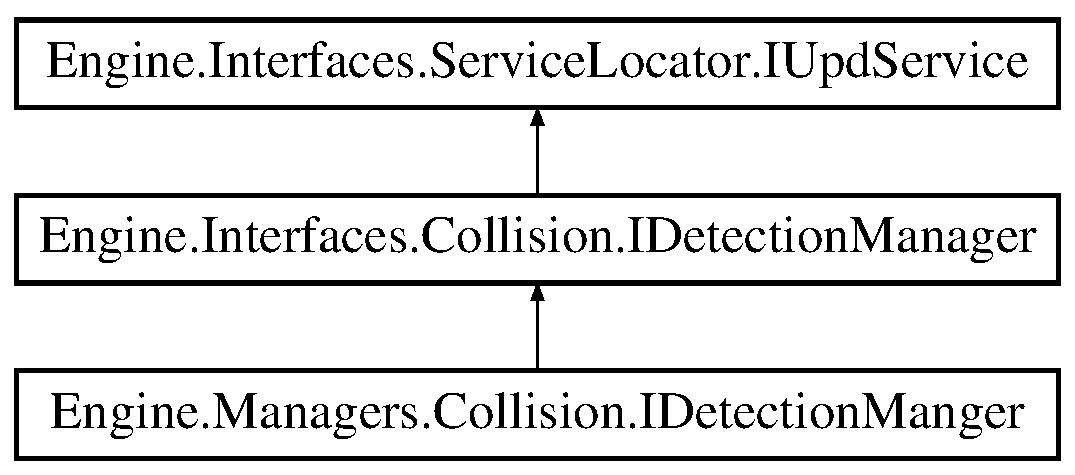
\includegraphics[height=3.000000cm]{d0/da2/a00502}
\end{center}
\end{figure}
\subsection*{Public Member Functions}
\begin{DoxyCompactItemize}
\item 
delegate void \hyperlink{a00502_a7a0a94d84fd7588d01218d607e7b1d27}{Collision\+Event\+Handler} (object sender, \hyperlink{a00350}{Collision\+Event\+Args} e)
\begin{DoxyCompactList}\small\item\em E\+V\+E\+NT\+: a reference to the Collision\+Event\+Handler which will be used when two objects collide \end{DoxyCompactList}\item 
void \hyperlink{a00502_ae4daf9d957c8b30e779a7ed89237b370}{add\+Collidable} (\hyperlink{a00426}{I\+Collidable} obj)
\begin{DoxyCompactList}\small\item\em M\+E\+T\+H\+OD\+: Adds an I\+C\+Ollidable to the list of objects to check \end{DoxyCompactList}\item 
void \hyperlink{a00502_ac032340610657f865bdd3b7a82e316c3}{Update} (Game\+Time game\+Time)
\begin{DoxyCompactList}\small\item\em M\+E\+T\+H\+OD\+: Called every frame of the game loop and contains all of the necessary code for the manager to calculate Whether each object is colliding or not \end{DoxyCompactList}\item 
void \hyperlink{a00502_a6785a08302cfe7d6fb08a7042691a3a8}{do\+Collision} ()
\begin{DoxyCompactList}\small\item\em M\+E\+T\+H\+OD\+: Checks A\+A\+BB \hyperlink{a00268}{Collision} for two objects \end{DoxyCompactList}\item 
void \hyperlink{a00502_a31a209d98a58cac4f6abd47711bf545c}{On\+A\+Collision} (\hyperlink{a00426}{I\+Collidable} A, \hyperlink{a00426}{I\+Collidable} B)
\begin{DoxyCompactList}\small\item\em M\+E\+T\+H\+OD\+: When two objects are colliding via A\+A\+BB collision, this method is called \end{DoxyCompactList}\item 
void \hyperlink{a00502_a272b97e8ab5caf3dcceb455849deb6ed}{Call\+S\+AT} (\hyperlink{a00426}{I\+Collidable} A, \hyperlink{a00426}{I\+Collidable} B, Vector2 mtv)
\begin{DoxyCompactList}\small\item\em M\+E\+T\+H\+OD\+: Call to fire an Event when S\+AT Calculates two shapes about to collide. \end{DoxyCompactList}\item 
void \hyperlink{a00502_a18f0056903776f291a462fb4bbbfc224}{Check\+S\+AT} (\hyperlink{a00426}{I\+Collidable} a, \hyperlink{a00426}{I\+Collidable} b)
\begin{DoxyCompactList}\small\item\em M\+E\+T\+H\+OD\+: Runs the S\+AT Calculations on two I\+Collidable objects and calls the event fire method when true. \end{DoxyCompactList}\item 
Vector2 \hyperlink{a00502_a47c9b58bdaf1f773ea3932f8c574ae0b}{Impulse\+Application} (\hyperlink{a00434}{I\+Hitbox} a, \hyperlink{a00434}{I\+Hitbox} b)
\begin{DoxyCompactList}\small\item\em M\+E\+T\+H\+OD\+: Applies the impulse to the two objects to simulate physics. \end{DoxyCompactList}\end{DoxyCompactItemize}
\subsection*{Events}
\begin{DoxyCompactItemize}
\item 
\hyperlink{a00502_a7a0a94d84fd7588d01218d607e7b1d27}{Collision\+Event\+Handler} \hyperlink{a00502_a030c2301f7a7ec14a4d852f3f039b22a}{On\+Collision}
\begin{DoxyCompactList}\small\item\em D\+E\+C\+L\+A\+RE\+: The event that will be fired once two objects collide \end{DoxyCompactList}\item 
\hyperlink{a00502_a7a0a94d84fd7588d01218d607e7b1d27}{Collision\+Event\+Handler} \hyperlink{a00502_a4eb9637ff1544210696df98bae59b07e}{On\+S\+A\+T\+Collision}
\begin{DoxyCompactList}\small\item\em D\+E\+C\+L\+A\+RE\+: The event that will be fired once two objects are calculated to collide or about to collide using the S\+AT method \end{DoxyCompactList}\end{DoxyCompactItemize}


\subsection{Detailed Description}
C\+L\+A\+SS\+: The Detection Manager is used for all collision calculations. Once two objects are colliding a \hyperlink{a00268}{Collision} event is fired with the necessary information for two objects to react properly. 



\subsection{Member Function Documentation}
\mbox{\Hypertarget{a00502_ae4daf9d957c8b30e779a7ed89237b370}\label{a00502_ae4daf9d957c8b30e779a7ed89237b370}} 
\index{Engine\+::\+Managers\+::\+Collision\+::\+I\+Detection\+Manger@{Engine\+::\+Managers\+::\+Collision\+::\+I\+Detection\+Manger}!add\+Collidable@{add\+Collidable}}
\index{add\+Collidable@{add\+Collidable}!Engine\+::\+Managers\+::\+Collision\+::\+I\+Detection\+Manger@{Engine\+::\+Managers\+::\+Collision\+::\+I\+Detection\+Manger}}
\subsubsection{\texorpdfstring{add\+Collidable()}{addCollidable()}}
{\footnotesize\ttfamily void Engine.\+Managers.\+Collision.\+I\+Detection\+Manger.\+add\+Collidable (\begin{DoxyParamCaption}\item[{\hyperlink{a00426}{I\+Collidable}}]{obj }\end{DoxyParamCaption})\hspace{0.3cm}{\ttfamily [inline]}}



M\+E\+T\+H\+OD\+: Adds an I\+C\+Ollidable to the list of objects to check 


\begin{DoxyParams}{Parameters}
{\em obj} & The object to add to the list\\
\hline
\end{DoxyParams}


Implements \hyperlink{a00430_a11808ec009ee682fa73e3c4ea6570139}{Engine.\+Interfaces.\+Collision.\+I\+Detection\+Manager}.

\mbox{\Hypertarget{a00502_a272b97e8ab5caf3dcceb455849deb6ed}\label{a00502_a272b97e8ab5caf3dcceb455849deb6ed}} 
\index{Engine\+::\+Managers\+::\+Collision\+::\+I\+Detection\+Manger@{Engine\+::\+Managers\+::\+Collision\+::\+I\+Detection\+Manger}!Call\+S\+AT@{Call\+S\+AT}}
\index{Call\+S\+AT@{Call\+S\+AT}!Engine\+::\+Managers\+::\+Collision\+::\+I\+Detection\+Manger@{Engine\+::\+Managers\+::\+Collision\+::\+I\+Detection\+Manger}}
\subsubsection{\texorpdfstring{Call\+S\+A\+T()}{CallSAT()}}
{\footnotesize\ttfamily void Engine.\+Managers.\+Collision.\+I\+Detection\+Manger.\+Call\+S\+AT (\begin{DoxyParamCaption}\item[{\hyperlink{a00426}{I\+Collidable}}]{A,  }\item[{\hyperlink{a00426}{I\+Collidable}}]{B,  }\item[{Vector2}]{mtv }\end{DoxyParamCaption})\hspace{0.3cm}{\ttfamily [inline]}}



M\+E\+T\+H\+OD\+: Call to fire an Event when S\+AT Calculates two shapes about to collide. 


\begin{DoxyParams}{Parameters}
{\em a} & Object A to be tested\\
\hline
{\em b} & Object B to be tested\\
\hline
{\em mtv} & \\
\hline
\end{DoxyParams}


Implements \hyperlink{a00430_ad87743faa9c3c212879716d7306c4fb3}{Engine.\+Interfaces.\+Collision.\+I\+Detection\+Manager}.

\mbox{\Hypertarget{a00502_a18f0056903776f291a462fb4bbbfc224}\label{a00502_a18f0056903776f291a462fb4bbbfc224}} 
\index{Engine\+::\+Managers\+::\+Collision\+::\+I\+Detection\+Manger@{Engine\+::\+Managers\+::\+Collision\+::\+I\+Detection\+Manger}!Check\+S\+AT@{Check\+S\+AT}}
\index{Check\+S\+AT@{Check\+S\+AT}!Engine\+::\+Managers\+::\+Collision\+::\+I\+Detection\+Manger@{Engine\+::\+Managers\+::\+Collision\+::\+I\+Detection\+Manger}}
\subsubsection{\texorpdfstring{Check\+S\+A\+T()}{CheckSAT()}}
{\footnotesize\ttfamily void Engine.\+Managers.\+Collision.\+I\+Detection\+Manger.\+Check\+S\+AT (\begin{DoxyParamCaption}\item[{\hyperlink{a00426}{I\+Collidable}}]{a,  }\item[{\hyperlink{a00426}{I\+Collidable}}]{b }\end{DoxyParamCaption})\hspace{0.3cm}{\ttfamily [inline]}}



M\+E\+T\+H\+OD\+: Runs the S\+AT Calculations on two I\+Collidable objects and calls the event fire method when true. 


\begin{DoxyParams}{Parameters}
{\em a} & Object A to be tested\\
\hline
{\em b} & Object B to be tested\\
\hline
\end{DoxyParams}
F\+OR\+: each hitbox on the first object

F\+OR\+: Each hitbox on the second object

IF\+: the S\+AT Calculation returns true

C\+A\+LL\+: Call\+S\+AT method which fires an Event and moves the objects out of each other

C\+A\+LL\+: Call\+S\+AT Method which fires an Event and applies an impule to each shape to simulate physics 

Implements \hyperlink{a00430_a1acd238daa104a8f4dcf36536e1ac9f9}{Engine.\+Interfaces.\+Collision.\+I\+Detection\+Manager}.

\mbox{\Hypertarget{a00502_a7a0a94d84fd7588d01218d607e7b1d27}\label{a00502_a7a0a94d84fd7588d01218d607e7b1d27}} 
\index{Engine\+::\+Managers\+::\+Collision\+::\+I\+Detection\+Manger@{Engine\+::\+Managers\+::\+Collision\+::\+I\+Detection\+Manger}!Collision\+Event\+Handler@{Collision\+Event\+Handler}}
\index{Collision\+Event\+Handler@{Collision\+Event\+Handler}!Engine\+::\+Managers\+::\+Collision\+::\+I\+Detection\+Manger@{Engine\+::\+Managers\+::\+Collision\+::\+I\+Detection\+Manger}}
\subsubsection{\texorpdfstring{Collision\+Event\+Handler()}{CollisionEventHandler()}}
{\footnotesize\ttfamily delegate void Engine.\+Managers.\+Collision.\+I\+Detection\+Manger.\+Collision\+Event\+Handler (\begin{DoxyParamCaption}\item[{object}]{sender,  }\item[{\hyperlink{a00350}{Collision\+Event\+Args}}]{e }\end{DoxyParamCaption})}



E\+V\+E\+NT\+: a reference to the Collision\+Event\+Handler which will be used when two objects collide 


\begin{DoxyParams}{Parameters}
{\em sender} & \\
\hline
{\em e} & \\
\hline
\end{DoxyParams}
\mbox{\Hypertarget{a00502_a6785a08302cfe7d6fb08a7042691a3a8}\label{a00502_a6785a08302cfe7d6fb08a7042691a3a8}} 
\index{Engine\+::\+Managers\+::\+Collision\+::\+I\+Detection\+Manger@{Engine\+::\+Managers\+::\+Collision\+::\+I\+Detection\+Manger}!do\+Collision@{do\+Collision}}
\index{do\+Collision@{do\+Collision}!Engine\+::\+Managers\+::\+Collision\+::\+I\+Detection\+Manger@{Engine\+::\+Managers\+::\+Collision\+::\+I\+Detection\+Manger}}
\subsubsection{\texorpdfstring{do\+Collision()}{doCollision()}}
{\footnotesize\ttfamily void Engine.\+Managers.\+Collision.\+I\+Detection\+Manger.\+do\+Collision (\begin{DoxyParamCaption}{ }\end{DoxyParamCaption})\hspace{0.3cm}{\ttfamily [inline]}}



M\+E\+T\+H\+OD\+: Checks A\+A\+BB \hyperlink{a00268}{Collision} for two objects 

I\+T\+E\+R\+A\+TE\+: through the list twice, counting one object above the first each time

IF\+: they\textquotesingle{}re not equal objects

S\+ET\+: the distance between the two objects

IF\+: there\textquotesingle{}s a collision, but also checks if A is a controller character, if so then it will move A around, otherwise tiles may have problems

S\+ET\+: Minimum Translation Vector

A\+DD minimum translation Vector to object. 

Implements \hyperlink{a00430_a139cca7ebb8b37ceba1bb1439cde83bf}{Engine.\+Interfaces.\+Collision.\+I\+Detection\+Manager}.

\mbox{\Hypertarget{a00502_a47c9b58bdaf1f773ea3932f8c574ae0b}\label{a00502_a47c9b58bdaf1f773ea3932f8c574ae0b}} 
\index{Engine\+::\+Managers\+::\+Collision\+::\+I\+Detection\+Manger@{Engine\+::\+Managers\+::\+Collision\+::\+I\+Detection\+Manger}!Impulse\+Application@{Impulse\+Application}}
\index{Impulse\+Application@{Impulse\+Application}!Engine\+::\+Managers\+::\+Collision\+::\+I\+Detection\+Manger@{Engine\+::\+Managers\+::\+Collision\+::\+I\+Detection\+Manger}}
\subsubsection{\texorpdfstring{Impulse\+Application()}{ImpulseApplication()}}
{\footnotesize\ttfamily Vector2 Engine.\+Managers.\+Collision.\+I\+Detection\+Manger.\+Impulse\+Application (\begin{DoxyParamCaption}\item[{\hyperlink{a00434}{I\+Hitbox}}]{a,  }\item[{\hyperlink{a00434}{I\+Hitbox}}]{b }\end{DoxyParamCaption})\hspace{0.3cm}{\ttfamily [inline]}}



M\+E\+T\+H\+OD\+: Applies the impulse to the two objects to simulate physics. 


\begin{DoxyParams}{Parameters}
{\em a} & Object A to be tested\\
\hline
{\em b} & Object B to be tested\\
\hline
\end{DoxyParams}
\begin{DoxyReturn}{Returns}
A Vector2 which will be applied to the object
\end{DoxyReturn}
D\+E\+C\+L\+A\+RE\+: The Combined velocity of the two objects

D\+E\+C\+L\+A\+RE\+: The closing normal which is the combined velocities proportionally adjusted so the Vector has a length of 1

D\+E\+C\+L\+A\+RE\+: T\+He dot product of the combined velocity and the \hyperlink{a00268}{Collision} Normal to get a Closing Velocity

M\+U\+L\+T\+I\+P\+LY\+: The collision normal by the closing velocity

R\+E\+T\+U\+RN\+: the collision normal. 

Implements \hyperlink{a00430_a853912077b127d7e6779accc914df3cf}{Engine.\+Interfaces.\+Collision.\+I\+Detection\+Manager}.

\mbox{\Hypertarget{a00502_a31a209d98a58cac4f6abd47711bf545c}\label{a00502_a31a209d98a58cac4f6abd47711bf545c}} 
\index{Engine\+::\+Managers\+::\+Collision\+::\+I\+Detection\+Manger@{Engine\+::\+Managers\+::\+Collision\+::\+I\+Detection\+Manger}!On\+A\+Collision@{On\+A\+Collision}}
\index{On\+A\+Collision@{On\+A\+Collision}!Engine\+::\+Managers\+::\+Collision\+::\+I\+Detection\+Manger@{Engine\+::\+Managers\+::\+Collision\+::\+I\+Detection\+Manger}}
\subsubsection{\texorpdfstring{On\+A\+Collision()}{OnACollision()}}
{\footnotesize\ttfamily void Engine.\+Managers.\+Collision.\+I\+Detection\+Manger.\+On\+A\+Collision (\begin{DoxyParamCaption}\item[{\hyperlink{a00426}{I\+Collidable}}]{A,  }\item[{\hyperlink{a00426}{I\+Collidable}}]{B }\end{DoxyParamCaption})\hspace{0.3cm}{\ttfamily [inline]}}



M\+E\+T\+H\+OD\+: When two objects are colliding via A\+A\+BB collision, this method is called 


\begin{DoxyParams}{Parameters}
{\em A} & The first object that\textquotesingle{}s colliding\\
\hline
{\em B} & The second object that\textquotesingle{}s colliding\\
\hline
\end{DoxyParams}
E\+V\+E\+NT\+: \hyperlink{a00268}{Collision} event with each shape. 

Implements \hyperlink{a00430_ac0f8278b5b5a1c103da46f154ad088dc}{Engine.\+Interfaces.\+Collision.\+I\+Detection\+Manager}.

\mbox{\Hypertarget{a00502_ac032340610657f865bdd3b7a82e316c3}\label{a00502_ac032340610657f865bdd3b7a82e316c3}} 
\index{Engine\+::\+Managers\+::\+Collision\+::\+I\+Detection\+Manger@{Engine\+::\+Managers\+::\+Collision\+::\+I\+Detection\+Manger}!Update@{Update}}
\index{Update@{Update}!Engine\+::\+Managers\+::\+Collision\+::\+I\+Detection\+Manger@{Engine\+::\+Managers\+::\+Collision\+::\+I\+Detection\+Manger}}
\subsubsection{\texorpdfstring{Update()}{Update()}}
{\footnotesize\ttfamily void Engine.\+Managers.\+Collision.\+I\+Detection\+Manger.\+Update (\begin{DoxyParamCaption}\item[{Game\+Time}]{game\+Time }\end{DoxyParamCaption})\hspace{0.3cm}{\ttfamily [inline]}}



M\+E\+T\+H\+OD\+: Called every frame of the game loop and contains all of the necessary code for the manager to calculate Whether each object is colliding or not 


\begin{DoxyParams}{Parameters}
{\em game\+Time} & Monogame Game\+Time\\
\hline
\end{DoxyParams}
F\+OR\+: each I\+Collidable in the collision list

F\+OR\+: Each I\+Collidable in the collision list

IF\+: The two objects are not the same thing

Run the S\+AT Calculation between the two objects. 

Implements \hyperlink{a00430_aeaa36b46e3ecd301b2fce9197fb0a35c}{Engine.\+Interfaces.\+Collision.\+I\+Detection\+Manager}.



\subsection{Event Documentation}
\mbox{\Hypertarget{a00502_a030c2301f7a7ec14a4d852f3f039b22a}\label{a00502_a030c2301f7a7ec14a4d852f3f039b22a}} 
\index{Engine\+::\+Managers\+::\+Collision\+::\+I\+Detection\+Manger@{Engine\+::\+Managers\+::\+Collision\+::\+I\+Detection\+Manger}!On\+Collision@{On\+Collision}}
\index{On\+Collision@{On\+Collision}!Engine\+::\+Managers\+::\+Collision\+::\+I\+Detection\+Manger@{Engine\+::\+Managers\+::\+Collision\+::\+I\+Detection\+Manger}}
\subsubsection{\texorpdfstring{On\+Collision}{OnCollision}}
{\footnotesize\ttfamily \hyperlink{a00502_a7a0a94d84fd7588d01218d607e7b1d27}{Collision\+Event\+Handler} Engine.\+Managers.\+Collision.\+I\+Detection\+Manger.\+On\+Collision}



D\+E\+C\+L\+A\+RE\+: The event that will be fired once two objects collide 

\mbox{\Hypertarget{a00502_a4eb9637ff1544210696df98bae59b07e}\label{a00502_a4eb9637ff1544210696df98bae59b07e}} 
\index{Engine\+::\+Managers\+::\+Collision\+::\+I\+Detection\+Manger@{Engine\+::\+Managers\+::\+Collision\+::\+I\+Detection\+Manger}!On\+S\+A\+T\+Collision@{On\+S\+A\+T\+Collision}}
\index{On\+S\+A\+T\+Collision@{On\+S\+A\+T\+Collision}!Engine\+::\+Managers\+::\+Collision\+::\+I\+Detection\+Manger@{Engine\+::\+Managers\+::\+Collision\+::\+I\+Detection\+Manger}}
\subsubsection{\texorpdfstring{On\+S\+A\+T\+Collision}{OnSATCollision}}
{\footnotesize\ttfamily \hyperlink{a00502_a7a0a94d84fd7588d01218d607e7b1d27}{Collision\+Event\+Handler} Engine.\+Managers.\+Collision.\+I\+Detection\+Manger.\+On\+S\+A\+T\+Collision}



D\+E\+C\+L\+A\+RE\+: The event that will be fired once two objects are calculated to collide or about to collide using the S\+AT method 



The documentation for this class was generated from the following file\+:\begin{DoxyCompactItemize}
\item 
\hyperlink{a00158}{Detection\+Manger.\+cs}\end{DoxyCompactItemize}

\hypertarget{a00454}{}\section{Engine.\+Interfaces.\+Render.\+I\+Drawable\+Component Interface Reference}
\label{a00454}\index{Engine.\+Interfaces.\+Render.\+I\+Drawable\+Component@{Engine.\+Interfaces.\+Render.\+I\+Drawable\+Component}}
Inheritance diagram for Engine.\+Interfaces.\+Render.\+I\+Drawable\+Component\+:\begin{figure}[H]
\begin{center}
\leavevmode
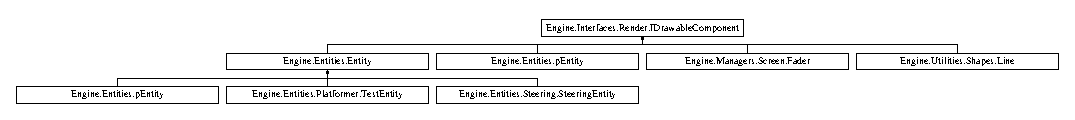
\includegraphics[height=1.166667cm]{d7/d9f/a00454}
\end{center}
\end{figure}
\subsection*{Public Member Functions}
\begin{DoxyCompactItemize}
\item 
void \hyperlink{a00454_a13aad31e3e179532915dbb93e91afaa3}{Draw} (Sprite\+Batch sprite\+Batch)
\end{DoxyCompactItemize}


\subsection{Member Function Documentation}
\mbox{\Hypertarget{a00454_a13aad31e3e179532915dbb93e91afaa3}\label{a00454_a13aad31e3e179532915dbb93e91afaa3}} 
\index{Engine\+::\+Interfaces\+::\+Render\+::\+I\+Drawable\+Component@{Engine\+::\+Interfaces\+::\+Render\+::\+I\+Drawable\+Component}!Draw@{Draw}}
\index{Draw@{Draw}!Engine\+::\+Interfaces\+::\+Render\+::\+I\+Drawable\+Component@{Engine\+::\+Interfaces\+::\+Render\+::\+I\+Drawable\+Component}}
\subsubsection{\texorpdfstring{Draw()}{Draw()}}
{\footnotesize\ttfamily void Engine.\+Interfaces.\+Render.\+I\+Drawable\+Component.\+Draw (\begin{DoxyParamCaption}\item[{Sprite\+Batch}]{sprite\+Batch }\end{DoxyParamCaption})}



Implemented in \hyperlink{a00314_a5c795930028c5672b54f95369b25019f}{Engine.\+Entities.\+Entity}, \hyperlink{a00534_a8a40165cf8a910849e01fb35b9567ee2}{Engine.\+Managers.\+Screen.\+Fader}, and \hyperlink{a00606_a8500392559da764797cdb92eb850a2ba}{Engine.\+Utilities.\+Shapes.\+Line}.



The documentation for this interface was generated from the following file\+:\begin{DoxyCompactItemize}
\item 
\hyperlink{a00122}{I\+Drawable\+Component.\+cs}\end{DoxyCompactItemize}

\hypertarget{a00438}{}\section{Engine.\+Interfaces.\+Entities.\+I\+Entity Interface Reference}
\label{a00438}\index{Engine.\+Interfaces.\+Entities.\+I\+Entity@{Engine.\+Interfaces.\+Entities.\+I\+Entity}}


I\+N\+T\+E\+R\+F\+A\+CE\+: An Interface that all entities must subscribe to and handles the implementation and properties for them.  


Inheritance diagram for Engine.\+Interfaces.\+Entities.\+I\+Entity\+:\begin{figure}[H]
\begin{center}
\leavevmode
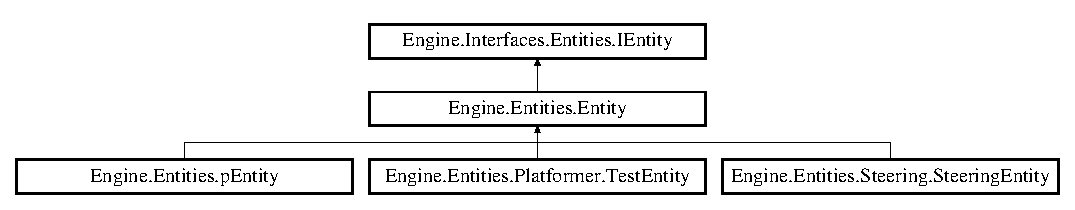
\includegraphics[height=2.372881cm]{dd/dfd/a00438}
\end{center}
\end{figure}
\subsection*{Public Member Functions}
\begin{DoxyCompactItemize}
\item 
void \hyperlink{a00438_a845918af6647460d2c47a3853a30f95f}{Draw} (Sprite\+Batch sprite\+Batch)
\begin{DoxyCompactList}\small\item\em M\+E\+T\+H\+OD\+: Draw \end{DoxyCompactList}\item 
void \hyperlink{a00438_a0c80525509aaeaa0d78eef908f7f7553}{Initialize} (Vector2 \hyperlink{a00438_a33bef4197ad7b1bf344ca31f0c1bed5b}{Position})
\begin{DoxyCompactList}\small\item\em M\+E\+T\+H\+OD\+: Initialise, give the Entity a position and texture \end{DoxyCompactList}\end{DoxyCompactItemize}
\subsection*{Properties}
\begin{DoxyCompactItemize}
\item 
Texture2D \hyperlink{a00438_a57d9471e7a098f07743eb215f7e7d07c}{Texture}\hspace{0.3cm}{\ttfamily  \mbox{[}get, set\mbox{]}}
\begin{DoxyCompactList}\small\item\em G\+ET\+: S\+ET\+: The Texture of the Entity \end{DoxyCompactList}\item 
Vector2 \hyperlink{a00438_a33bef4197ad7b1bf344ca31f0c1bed5b}{Position}\hspace{0.3cm}{\ttfamily  \mbox{[}get, set\mbox{]}}
\begin{DoxyCompactList}\small\item\em G\+ET\+: S\+ET\+: The Position of the Entity \end{DoxyCompactList}\item 
Vector2 \hyperlink{a00438_a6569977576ff585b7a883f11fc073a6d}{Velocity}\hspace{0.3cm}{\ttfamily  \mbox{[}get\mbox{]}}
\begin{DoxyCompactList}\small\item\em G\+ET\+: The velocity of the Entity \end{DoxyCompactList}\item 
int \hyperlink{a00438_af60396008872673e4a81baab29ad91b1}{Unique\+ID}\hspace{0.3cm}{\ttfamily  \mbox{[}get\mbox{]}}
\begin{DoxyCompactList}\small\item\em G\+ET\+: The unique ID for the Entity \end{DoxyCompactList}\item 
Rectangle \hyperlink{a00438_a0c45df802f74c4910b8e7a0842cfbcd2}{Bounds}\hspace{0.3cm}{\ttfamily  \mbox{[}get\mbox{]}}
\begin{DoxyCompactList}\small\item\em G\+ET\+: An Axis aligned bounding box for the bounds of the Entity. \end{DoxyCompactList}\item 
bool \hyperlink{a00438_a5f3ad8367eed3ba92165cea56d62eaf8}{is\+Collidable}\hspace{0.3cm}{\ttfamily  \mbox{[}get, set\mbox{]}}
\begin{DoxyCompactList}\small\item\em G\+ET\+: S\+ET\+: A boolean to state whether the entity needs to be included in any calculations for collision \end{DoxyCompactList}\item 
bool \hyperlink{a00438_a6aa73f86c947c5c215b45f8f0cadb234}{is\+Visible}\hspace{0.3cm}{\ttfamily  \mbox{[}get, set\mbox{]}}
\begin{DoxyCompactList}\small\item\em G\+ET\+: S\+ET\+: A Boolean for whether the entity needs to be drawn. \end{DoxyCompactList}\item 
string \hyperlink{a00438_a7a3927fc2320652f20b86e68544bc571}{Name}\hspace{0.3cm}{\ttfamily  \mbox{[}get, set\mbox{]}}
\begin{DoxyCompactList}\small\item\em G\+ET\+: S\+ET\+: The name of the Entity. \end{DoxyCompactList}\end{DoxyCompactItemize}


\subsection{Detailed Description}
I\+N\+T\+E\+R\+F\+A\+CE\+: An Interface that all entities must subscribe to and handles the implementation and properties for them. 



\subsection{Member Function Documentation}
\mbox{\Hypertarget{a00438_a845918af6647460d2c47a3853a30f95f}\label{a00438_a845918af6647460d2c47a3853a30f95f}} 
\index{Engine\+::\+Interfaces\+::\+Entities\+::\+I\+Entity@{Engine\+::\+Interfaces\+::\+Entities\+::\+I\+Entity}!Draw@{Draw}}
\index{Draw@{Draw}!Engine\+::\+Interfaces\+::\+Entities\+::\+I\+Entity@{Engine\+::\+Interfaces\+::\+Entities\+::\+I\+Entity}}
\subsubsection{\texorpdfstring{Draw()}{Draw()}}
{\footnotesize\ttfamily void Engine.\+Interfaces.\+Entities.\+I\+Entity.\+Draw (\begin{DoxyParamCaption}\item[{Sprite\+Batch}]{sprite\+Batch }\end{DoxyParamCaption})}



M\+E\+T\+H\+OD\+: Draw 


\begin{DoxyParams}{Parameters}
{\em sprite\+Batch} & \\
\hline
\end{DoxyParams}


Implemented in \hyperlink{a00314_a5c795930028c5672b54f95369b25019f}{Engine.\+Entities.\+Entity}.

\mbox{\Hypertarget{a00438_a0c80525509aaeaa0d78eef908f7f7553}\label{a00438_a0c80525509aaeaa0d78eef908f7f7553}} 
\index{Engine\+::\+Interfaces\+::\+Entities\+::\+I\+Entity@{Engine\+::\+Interfaces\+::\+Entities\+::\+I\+Entity}!Initialize@{Initialize}}
\index{Initialize@{Initialize}!Engine\+::\+Interfaces\+::\+Entities\+::\+I\+Entity@{Engine\+::\+Interfaces\+::\+Entities\+::\+I\+Entity}}
\subsubsection{\texorpdfstring{Initialize()}{Initialize()}}
{\footnotesize\ttfamily void Engine.\+Interfaces.\+Entities.\+I\+Entity.\+Initialize (\begin{DoxyParamCaption}\item[{Vector2}]{Position }\end{DoxyParamCaption})}



M\+E\+T\+H\+OD\+: Initialise, give the Entity a position and texture 


\begin{DoxyParams}{Parameters}
{\em Position} & \\
\hline
\end{DoxyParams}


Implemented in \hyperlink{a00314_aa1425aeeac379c5141e7560b84850b3d}{Engine.\+Entities.\+Entity}, \hyperlink{a00322_aad953baa984c0f958d3e96efbfc3bca9}{Engine.\+Entities.\+p\+Entity}, \hyperlink{a00330_ad4122c4f38d98746a67532d0a6836da5}{Engine.\+Entities.\+Platformer.\+Test\+Entity}, and \hyperlink{a00342_a7b1e3df5320c999d2cf1cc3b97994401}{Engine.\+Entities.\+Steering.\+Steering\+Entity}.



\subsection{Property Documentation}
\mbox{\Hypertarget{a00438_a0c45df802f74c4910b8e7a0842cfbcd2}\label{a00438_a0c45df802f74c4910b8e7a0842cfbcd2}} 
\index{Engine\+::\+Interfaces\+::\+Entities\+::\+I\+Entity@{Engine\+::\+Interfaces\+::\+Entities\+::\+I\+Entity}!Bounds@{Bounds}}
\index{Bounds@{Bounds}!Engine\+::\+Interfaces\+::\+Entities\+::\+I\+Entity@{Engine\+::\+Interfaces\+::\+Entities\+::\+I\+Entity}}
\subsubsection{\texorpdfstring{Bounds}{Bounds}}
{\footnotesize\ttfamily Rectangle Engine.\+Interfaces.\+Entities.\+I\+Entity.\+Bounds\hspace{0.3cm}{\ttfamily [get]}}



G\+ET\+: An Axis aligned bounding box for the bounds of the Entity. 

\mbox{\Hypertarget{a00438_a5f3ad8367eed3ba92165cea56d62eaf8}\label{a00438_a5f3ad8367eed3ba92165cea56d62eaf8}} 
\index{Engine\+::\+Interfaces\+::\+Entities\+::\+I\+Entity@{Engine\+::\+Interfaces\+::\+Entities\+::\+I\+Entity}!is\+Collidable@{is\+Collidable}}
\index{is\+Collidable@{is\+Collidable}!Engine\+::\+Interfaces\+::\+Entities\+::\+I\+Entity@{Engine\+::\+Interfaces\+::\+Entities\+::\+I\+Entity}}
\subsubsection{\texorpdfstring{is\+Collidable}{isCollidable}}
{\footnotesize\ttfamily bool Engine.\+Interfaces.\+Entities.\+I\+Entity.\+is\+Collidable\hspace{0.3cm}{\ttfamily [get]}, {\ttfamily [set]}}



G\+ET\+: S\+ET\+: A boolean to state whether the entity needs to be included in any calculations for collision 

\mbox{\Hypertarget{a00438_a6aa73f86c947c5c215b45f8f0cadb234}\label{a00438_a6aa73f86c947c5c215b45f8f0cadb234}} 
\index{Engine\+::\+Interfaces\+::\+Entities\+::\+I\+Entity@{Engine\+::\+Interfaces\+::\+Entities\+::\+I\+Entity}!is\+Visible@{is\+Visible}}
\index{is\+Visible@{is\+Visible}!Engine\+::\+Interfaces\+::\+Entities\+::\+I\+Entity@{Engine\+::\+Interfaces\+::\+Entities\+::\+I\+Entity}}
\subsubsection{\texorpdfstring{is\+Visible}{isVisible}}
{\footnotesize\ttfamily bool Engine.\+Interfaces.\+Entities.\+I\+Entity.\+is\+Visible\hspace{0.3cm}{\ttfamily [get]}, {\ttfamily [set]}}



G\+ET\+: S\+ET\+: A Boolean for whether the entity needs to be drawn. 

\mbox{\Hypertarget{a00438_a7a3927fc2320652f20b86e68544bc571}\label{a00438_a7a3927fc2320652f20b86e68544bc571}} 
\index{Engine\+::\+Interfaces\+::\+Entities\+::\+I\+Entity@{Engine\+::\+Interfaces\+::\+Entities\+::\+I\+Entity}!Name@{Name}}
\index{Name@{Name}!Engine\+::\+Interfaces\+::\+Entities\+::\+I\+Entity@{Engine\+::\+Interfaces\+::\+Entities\+::\+I\+Entity}}
\subsubsection{\texorpdfstring{Name}{Name}}
{\footnotesize\ttfamily string Engine.\+Interfaces.\+Entities.\+I\+Entity.\+Name\hspace{0.3cm}{\ttfamily [get]}, {\ttfamily [set]}}



G\+ET\+: S\+ET\+: The name of the Entity. 

\mbox{\Hypertarget{a00438_a33bef4197ad7b1bf344ca31f0c1bed5b}\label{a00438_a33bef4197ad7b1bf344ca31f0c1bed5b}} 
\index{Engine\+::\+Interfaces\+::\+Entities\+::\+I\+Entity@{Engine\+::\+Interfaces\+::\+Entities\+::\+I\+Entity}!Position@{Position}}
\index{Position@{Position}!Engine\+::\+Interfaces\+::\+Entities\+::\+I\+Entity@{Engine\+::\+Interfaces\+::\+Entities\+::\+I\+Entity}}
\subsubsection{\texorpdfstring{Position}{Position}}
{\footnotesize\ttfamily Vector2 Engine.\+Interfaces.\+Entities.\+I\+Entity.\+Position\hspace{0.3cm}{\ttfamily [get]}, {\ttfamily [set]}}



G\+ET\+: S\+ET\+: The Position of the Entity 

\mbox{\Hypertarget{a00438_a57d9471e7a098f07743eb215f7e7d07c}\label{a00438_a57d9471e7a098f07743eb215f7e7d07c}} 
\index{Engine\+::\+Interfaces\+::\+Entities\+::\+I\+Entity@{Engine\+::\+Interfaces\+::\+Entities\+::\+I\+Entity}!Texture@{Texture}}
\index{Texture@{Texture}!Engine\+::\+Interfaces\+::\+Entities\+::\+I\+Entity@{Engine\+::\+Interfaces\+::\+Entities\+::\+I\+Entity}}
\subsubsection{\texorpdfstring{Texture}{Texture}}
{\footnotesize\ttfamily Texture2D Engine.\+Interfaces.\+Entities.\+I\+Entity.\+Texture\hspace{0.3cm}{\ttfamily [get]}, {\ttfamily [set]}}



G\+ET\+: S\+ET\+: The Texture of the Entity 

\mbox{\Hypertarget{a00438_af60396008872673e4a81baab29ad91b1}\label{a00438_af60396008872673e4a81baab29ad91b1}} 
\index{Engine\+::\+Interfaces\+::\+Entities\+::\+I\+Entity@{Engine\+::\+Interfaces\+::\+Entities\+::\+I\+Entity}!Unique\+ID@{Unique\+ID}}
\index{Unique\+ID@{Unique\+ID}!Engine\+::\+Interfaces\+::\+Entities\+::\+I\+Entity@{Engine\+::\+Interfaces\+::\+Entities\+::\+I\+Entity}}
\subsubsection{\texorpdfstring{Unique\+ID}{UniqueID}}
{\footnotesize\ttfamily int Engine.\+Interfaces.\+Entities.\+I\+Entity.\+Unique\+ID\hspace{0.3cm}{\ttfamily [get]}}



G\+ET\+: The unique ID for the Entity 

\mbox{\Hypertarget{a00438_a6569977576ff585b7a883f11fc073a6d}\label{a00438_a6569977576ff585b7a883f11fc073a6d}} 
\index{Engine\+::\+Interfaces\+::\+Entities\+::\+I\+Entity@{Engine\+::\+Interfaces\+::\+Entities\+::\+I\+Entity}!Velocity@{Velocity}}
\index{Velocity@{Velocity}!Engine\+::\+Interfaces\+::\+Entities\+::\+I\+Entity@{Engine\+::\+Interfaces\+::\+Entities\+::\+I\+Entity}}
\subsubsection{\texorpdfstring{Velocity}{Velocity}}
{\footnotesize\ttfamily Vector2 Engine.\+Interfaces.\+Entities.\+I\+Entity.\+Velocity\hspace{0.3cm}{\ttfamily [get]}}



G\+ET\+: The velocity of the Entity 



The documentation for this interface was generated from the following file\+:\begin{DoxyCompactItemize}
\item 
\hyperlink{a00110}{I\+Entity.\+cs}\end{DoxyCompactItemize}

\hypertarget{a00442}{}\section{Engine.\+Interfaces.\+Entities.\+I\+Entity\+Manager Interface Reference}
\label{a00442}\index{Engine.\+Interfaces.\+Entities.\+I\+Entity\+Manager@{Engine.\+Interfaces.\+Entities.\+I\+Entity\+Manager}}


I\+N\+T\+E\+R\+F\+A\+CE\+: R\+Esponsible for the implementation found in Entity\+Manager which is responsible for adding and removing entities from the game scene  


Inheritance diagram for Engine.\+Interfaces.\+Entities.\+I\+Entity\+Manager\+:\begin{figure}[H]
\begin{center}
\leavevmode
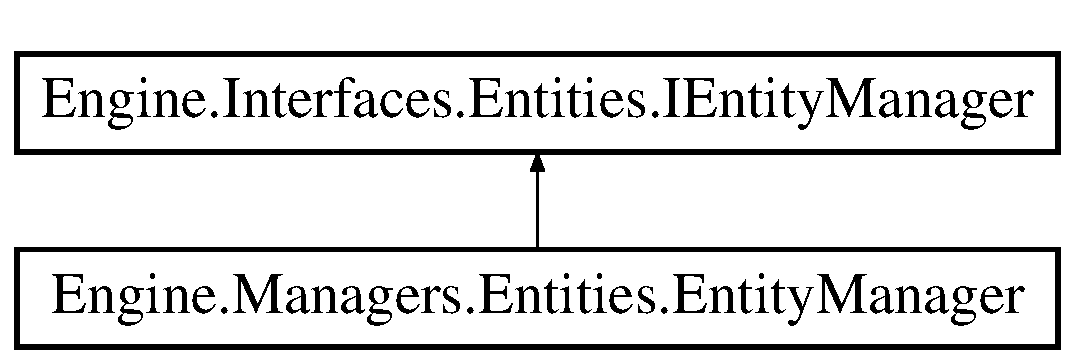
\includegraphics[height=2.000000cm]{db/d34/a00442}
\end{center}
\end{figure}
\subsection*{Public Member Functions}
\begin{DoxyCompactItemize}
\item 
List$<$ \hyperlink{a00438}{I\+Entity} $>$ \hyperlink{a00442_a8f71921098ae85f7f504f61a399a1bd8}{get\+List} ()
\begin{DoxyCompactList}\small\item\em M\+E\+T\+H\+OD\+: returns a list of entities \end{DoxyCompactList}\item 
List$<$ \hyperlink{a00438}{I\+Entity} $>$ \hyperlink{a00442_a6a6229acffece1f804ba440cf847820d}{get\+Cam\+List} ()
\begin{DoxyCompactList}\small\item\em M\+E\+T\+H\+OD\+: Returns a list of entities requiring a camera \end{DoxyCompactList}\item 
void \hyperlink{a00442_af229fa3936a8483383bb7ddd5b4184b0}{add\+Entity} (\hyperlink{a00438}{I\+Entity} e)
\begin{DoxyCompactList}\small\item\em M\+E\+T\+H\+OD\+: Add an entity to the list of entities \end{DoxyCompactList}\item 
void \hyperlink{a00442_a37055c1d97dd8da61a53a2b0683df54d}{add\+Cam\+Entity} (\hyperlink{a00438}{I\+Entity} e)
\begin{DoxyCompactList}\small\item\em M\+E\+T\+H\+OD\+: Add an entity requiring a camera to the list of entities \end{DoxyCompactList}\item 
\hyperlink{a00438}{I\+Entity} \hyperlink{a00442_a8f746b319d35a76cb4cdb1853f3069ed}{create\+Entity$<$ T $>$} (Vector2 Position)
\begin{DoxyCompactList}\small\item\em M\+E\+T\+H\+OD\+: Create a new \hyperlink{a00438}{I\+Entity} and add it to the list of I\+Entities \end{DoxyCompactList}\item 
\hyperlink{a00438}{I\+Entity} \hyperlink{a00442_aad35a164d944dcb7af20470bac0d3351}{create\+Entity\+Cam\+Drawable$<$ T $>$} (Vector2 Position)
\begin{DoxyCompactList}\small\item\em M\+E\+T\+H\+OD\+: Create a new \hyperlink{a00438}{I\+Entity} requiring a Camera and add it to the list of I\+Entites \end{DoxyCompactList}\item 
\hyperlink{a00438}{I\+Entity} \hyperlink{a00442_a36f4ce84282acb366896ebec20677cce}{create\+Entity\+Drawable$<$ T $>$} (Vector2 Position)
\begin{DoxyCompactList}\small\item\em M\+E\+T\+H\+OD\+: Create a new Drawable \hyperlink{a00438}{I\+Entity} and add it to the list of I\+Entities \end{DoxyCompactList}\item 
void \hyperlink{a00442_a04101871e7eef6b222a0cbd6225d0a7a}{temp\+Cam\+Clear} ()
\begin{DoxyCompactList}\small\item\em M\+E\+T\+H\+OD\+: Clear all Camera entities \end{DoxyCompactList}\item 
void \hyperlink{a00442_adff1edf326874f25e8a90bf45f020120}{get\+Entity} (string name)
\begin{DoxyCompactList}\small\item\em M\+E\+T\+H\+OD\+: Get an entity by it\textquotesingle{}s name \end{DoxyCompactList}\item 
\hyperlink{a00438}{I\+Entity} \hyperlink{a00442_aa1098871f43bbd775954aea10a958c0b}{get\+Cam\+Entity} (string name)
\begin{DoxyCompactList}\small\item\em M\+E\+T\+H\+OD\+: Get a Camera \hyperlink{a00438}{I\+Entity} by it;s name \end{DoxyCompactList}\item 
void \hyperlink{a00442_acccc889cc99843899ce0652a9959e907}{clear\+List} ()
\begin{DoxyCompactList}\small\item\em M\+E\+T\+H\+OD\+: Clear the list of all I\+Entities \end{DoxyCompactList}\item 
void \hyperlink{a00442_a13b425137cec67f2df4e65e8d08c531b}{remove\+Entity} (int entity\+ID)
\begin{DoxyCompactList}\small\item\em M\+E\+T\+H\+OD\+: Remove a specific \hyperlink{a00438}{I\+Entity} from the manager and list of Ientities \end{DoxyCompactList}\item 
void \hyperlink{a00442_aa341696fc31e28c71448cef613bf7f30}{remove\+Cam\+Entity} (int entity\+ID)
\begin{DoxyCompactList}\small\item\em M\+E\+T\+H\+OD\+: Remove a specific Camera entity by it;s ID \end{DoxyCompactList}\item 
void \hyperlink{a00442_a1b5aeaf8f2f6ad4a0c93aec1c331c1b2}{Update} (Game\+Time game\+Time)
\begin{DoxyCompactList}\small\item\em M\+E\+T\+H\+OD\+: The Update loop that is called every frame \end{DoxyCompactList}\end{DoxyCompactItemize}


\subsection{Detailed Description}
I\+N\+T\+E\+R\+F\+A\+CE\+: R\+Esponsible for the implementation found in Entity\+Manager which is responsible for adding and removing entities from the game scene 



\subsection{Member Function Documentation}
\mbox{\Hypertarget{a00442_a37055c1d97dd8da61a53a2b0683df54d}\label{a00442_a37055c1d97dd8da61a53a2b0683df54d}} 
\index{Engine\+::\+Interfaces\+::\+Entities\+::\+I\+Entity\+Manager@{Engine\+::\+Interfaces\+::\+Entities\+::\+I\+Entity\+Manager}!add\+Cam\+Entity@{add\+Cam\+Entity}}
\index{add\+Cam\+Entity@{add\+Cam\+Entity}!Engine\+::\+Interfaces\+::\+Entities\+::\+I\+Entity\+Manager@{Engine\+::\+Interfaces\+::\+Entities\+::\+I\+Entity\+Manager}}
\subsubsection{\texorpdfstring{add\+Cam\+Entity()}{addCamEntity()}}
{\footnotesize\ttfamily void Engine.\+Interfaces.\+Entities.\+I\+Entity\+Manager.\+add\+Cam\+Entity (\begin{DoxyParamCaption}\item[{\hyperlink{a00438}{I\+Entity}}]{e }\end{DoxyParamCaption})}



M\+E\+T\+H\+OD\+: Add an entity requiring a camera to the list of entities 


\begin{DoxyParams}{Parameters}
{\em e} & The entity to be added to the camera entity list\\
\hline
\end{DoxyParams}


Implemented in \hyperlink{a00518_a5b84d299c11d42065f55048dd14fdd4c}{Engine.\+Managers.\+Entities.\+Entity\+Manager}.

\mbox{\Hypertarget{a00442_af229fa3936a8483383bb7ddd5b4184b0}\label{a00442_af229fa3936a8483383bb7ddd5b4184b0}} 
\index{Engine\+::\+Interfaces\+::\+Entities\+::\+I\+Entity\+Manager@{Engine\+::\+Interfaces\+::\+Entities\+::\+I\+Entity\+Manager}!add\+Entity@{add\+Entity}}
\index{add\+Entity@{add\+Entity}!Engine\+::\+Interfaces\+::\+Entities\+::\+I\+Entity\+Manager@{Engine\+::\+Interfaces\+::\+Entities\+::\+I\+Entity\+Manager}}
\subsubsection{\texorpdfstring{add\+Entity()}{addEntity()}}
{\footnotesize\ttfamily void Engine.\+Interfaces.\+Entities.\+I\+Entity\+Manager.\+add\+Entity (\begin{DoxyParamCaption}\item[{\hyperlink{a00438}{I\+Entity}}]{e }\end{DoxyParamCaption})}



M\+E\+T\+H\+OD\+: Add an entity to the list of entities 


\begin{DoxyParams}{Parameters}
{\em e} & The entity to be added to the list\\
\hline
\end{DoxyParams}


Implemented in \hyperlink{a00518_a33cf4a636f70486e8a13c52bb4395cd6}{Engine.\+Managers.\+Entities.\+Entity\+Manager}.

\mbox{\Hypertarget{a00442_acccc889cc99843899ce0652a9959e907}\label{a00442_acccc889cc99843899ce0652a9959e907}} 
\index{Engine\+::\+Interfaces\+::\+Entities\+::\+I\+Entity\+Manager@{Engine\+::\+Interfaces\+::\+Entities\+::\+I\+Entity\+Manager}!clear\+List@{clear\+List}}
\index{clear\+List@{clear\+List}!Engine\+::\+Interfaces\+::\+Entities\+::\+I\+Entity\+Manager@{Engine\+::\+Interfaces\+::\+Entities\+::\+I\+Entity\+Manager}}
\subsubsection{\texorpdfstring{clear\+List()}{clearList()}}
{\footnotesize\ttfamily void Engine.\+Interfaces.\+Entities.\+I\+Entity\+Manager.\+clear\+List (\begin{DoxyParamCaption}{ }\end{DoxyParamCaption})}



M\+E\+T\+H\+OD\+: Clear the list of all I\+Entities 



Implemented in \hyperlink{a00518_a4eff29b463061f602be758bd3d36ef25}{Engine.\+Managers.\+Entities.\+Entity\+Manager}.

\mbox{\Hypertarget{a00442_a8f746b319d35a76cb4cdb1853f3069ed}\label{a00442_a8f746b319d35a76cb4cdb1853f3069ed}} 
\index{Engine\+::\+Interfaces\+::\+Entities\+::\+I\+Entity\+Manager@{Engine\+::\+Interfaces\+::\+Entities\+::\+I\+Entity\+Manager}!create\+Entity$<$ T $>$@{create\+Entity$<$ T $>$}}
\index{create\+Entity$<$ T $>$@{create\+Entity$<$ T $>$}!Engine\+::\+Interfaces\+::\+Entities\+::\+I\+Entity\+Manager@{Engine\+::\+Interfaces\+::\+Entities\+::\+I\+Entity\+Manager}}
\subsubsection{\texorpdfstring{create\+Entity$<$ T $>$()}{createEntity< T >()}}
{\footnotesize\ttfamily \hyperlink{a00438}{I\+Entity} Engine.\+Interfaces.\+Entities.\+I\+Entity\+Manager.\+create\+Entity$<$ T $>$ (\begin{DoxyParamCaption}\item[{Vector2}]{Position }\end{DoxyParamCaption})}



M\+E\+T\+H\+OD\+: Create a new \hyperlink{a00438}{I\+Entity} and add it to the list of I\+Entities 


\begin{DoxyTemplParams}{Template Parameters}
{\em T} & A generic type of entity to be created\\
\hline
\end{DoxyTemplParams}

\begin{DoxyParams}{Parameters}
{\em Position} & the position this entity will be initialised at\\
\hline
\end{DoxyParams}
\begin{DoxyReturn}{Returns}

\end{DoxyReturn}


Implemented in \hyperlink{a00518_a228280a4515648318fb5528936249a8b}{Engine.\+Managers.\+Entities.\+Entity\+Manager}.

\begin{Desc}
\item[Type Constraints]\begin{description}
\item[{\em T} : {\em I\+Entity}]\item[{\em T} : {\em new()}]\end{description}
\end{Desc}
\mbox{\Hypertarget{a00442_aad35a164d944dcb7af20470bac0d3351}\label{a00442_aad35a164d944dcb7af20470bac0d3351}} 
\index{Engine\+::\+Interfaces\+::\+Entities\+::\+I\+Entity\+Manager@{Engine\+::\+Interfaces\+::\+Entities\+::\+I\+Entity\+Manager}!create\+Entity\+Cam\+Drawable$<$ T $>$@{create\+Entity\+Cam\+Drawable$<$ T $>$}}
\index{create\+Entity\+Cam\+Drawable$<$ T $>$@{create\+Entity\+Cam\+Drawable$<$ T $>$}!Engine\+::\+Interfaces\+::\+Entities\+::\+I\+Entity\+Manager@{Engine\+::\+Interfaces\+::\+Entities\+::\+I\+Entity\+Manager}}
\subsubsection{\texorpdfstring{create\+Entity\+Cam\+Drawable$<$ T $>$()}{createEntityCamDrawable< T >()}}
{\footnotesize\ttfamily \hyperlink{a00438}{I\+Entity} Engine.\+Interfaces.\+Entities.\+I\+Entity\+Manager.\+create\+Entity\+Cam\+Drawable$<$ T $>$ (\begin{DoxyParamCaption}\item[{Vector2}]{Position }\end{DoxyParamCaption})}



M\+E\+T\+H\+OD\+: Create a new \hyperlink{a00438}{I\+Entity} requiring a Camera and add it to the list of I\+Entites 


\begin{DoxyTemplParams}{Template Parameters}
{\em T} & The generic type of entity to be created\\
\hline
\end{DoxyTemplParams}

\begin{DoxyParams}{Parameters}
{\em Position} & the position the entity will be initialised at\\
\hline
\end{DoxyParams}
\begin{DoxyReturn}{Returns}

\end{DoxyReturn}


Implemented in \hyperlink{a00518_a89ca1b1834aff0dc1d2c6ec95dcd0793}{Engine.\+Managers.\+Entities.\+Entity\+Manager}.

\begin{Desc}
\item[Type Constraints]\begin{description}
\item[{\em T} : {\em I\+Entity}]\item[{\em T} : {\em new()}]\end{description}
\end{Desc}
\mbox{\Hypertarget{a00442_a36f4ce84282acb366896ebec20677cce}\label{a00442_a36f4ce84282acb366896ebec20677cce}} 
\index{Engine\+::\+Interfaces\+::\+Entities\+::\+I\+Entity\+Manager@{Engine\+::\+Interfaces\+::\+Entities\+::\+I\+Entity\+Manager}!create\+Entity\+Drawable$<$ T $>$@{create\+Entity\+Drawable$<$ T $>$}}
\index{create\+Entity\+Drawable$<$ T $>$@{create\+Entity\+Drawable$<$ T $>$}!Engine\+::\+Interfaces\+::\+Entities\+::\+I\+Entity\+Manager@{Engine\+::\+Interfaces\+::\+Entities\+::\+I\+Entity\+Manager}}
\subsubsection{\texorpdfstring{create\+Entity\+Drawable$<$ T $>$()}{createEntityDrawable< T >()}}
{\footnotesize\ttfamily \hyperlink{a00438}{I\+Entity} Engine.\+Interfaces.\+Entities.\+I\+Entity\+Manager.\+create\+Entity\+Drawable$<$ T $>$ (\begin{DoxyParamCaption}\item[{Vector2}]{Position }\end{DoxyParamCaption})}



M\+E\+T\+H\+OD\+: Create a new Drawable \hyperlink{a00438}{I\+Entity} and add it to the list of I\+Entities 


\begin{DoxyTemplParams}{Template Parameters}
{\em T} & The generic type of entity to be created\\
\hline
\end{DoxyTemplParams}

\begin{DoxyParams}{Parameters}
{\em Position} & the position the entity will be initialised at\\
\hline
\end{DoxyParams}
\begin{DoxyReturn}{Returns}

\end{DoxyReturn}


Implemented in \hyperlink{a00518_a787212a79eb20bd2c695783b5f802347}{Engine.\+Managers.\+Entities.\+Entity\+Manager}.

\begin{Desc}
\item[Type Constraints]\begin{description}
\item[{\em T} : {\em I\+Entity}]\item[{\em T} : {\em new()}]\end{description}
\end{Desc}
\mbox{\Hypertarget{a00442_aa1098871f43bbd775954aea10a958c0b}\label{a00442_aa1098871f43bbd775954aea10a958c0b}} 
\index{Engine\+::\+Interfaces\+::\+Entities\+::\+I\+Entity\+Manager@{Engine\+::\+Interfaces\+::\+Entities\+::\+I\+Entity\+Manager}!get\+Cam\+Entity@{get\+Cam\+Entity}}
\index{get\+Cam\+Entity@{get\+Cam\+Entity}!Engine\+::\+Interfaces\+::\+Entities\+::\+I\+Entity\+Manager@{Engine\+::\+Interfaces\+::\+Entities\+::\+I\+Entity\+Manager}}
\subsubsection{\texorpdfstring{get\+Cam\+Entity()}{getCamEntity()}}
{\footnotesize\ttfamily \hyperlink{a00438}{I\+Entity} Engine.\+Interfaces.\+Entities.\+I\+Entity\+Manager.\+get\+Cam\+Entity (\begin{DoxyParamCaption}\item[{string}]{name }\end{DoxyParamCaption})}



M\+E\+T\+H\+OD\+: Get a Camera \hyperlink{a00438}{I\+Entity} by it;s name 


\begin{DoxyParams}{Parameters}
{\em name} & The name of the entity to be returned\\
\hline
\end{DoxyParams}
\begin{DoxyReturn}{Returns}
\hyperlink{a00438}{I\+Entity}
\end{DoxyReturn}


Implemented in \hyperlink{a00518_ab3ff805a060af38748444e520995d8fa}{Engine.\+Managers.\+Entities.\+Entity\+Manager}.

\mbox{\Hypertarget{a00442_a6a6229acffece1f804ba440cf847820d}\label{a00442_a6a6229acffece1f804ba440cf847820d}} 
\index{Engine\+::\+Interfaces\+::\+Entities\+::\+I\+Entity\+Manager@{Engine\+::\+Interfaces\+::\+Entities\+::\+I\+Entity\+Manager}!get\+Cam\+List@{get\+Cam\+List}}
\index{get\+Cam\+List@{get\+Cam\+List}!Engine\+::\+Interfaces\+::\+Entities\+::\+I\+Entity\+Manager@{Engine\+::\+Interfaces\+::\+Entities\+::\+I\+Entity\+Manager}}
\subsubsection{\texorpdfstring{get\+Cam\+List()}{getCamList()}}
{\footnotesize\ttfamily List$<$\hyperlink{a00438}{I\+Entity}$>$ Engine.\+Interfaces.\+Entities.\+I\+Entity\+Manager.\+get\+Cam\+List (\begin{DoxyParamCaption}{ }\end{DoxyParamCaption})}



M\+E\+T\+H\+OD\+: Returns a list of entities requiring a camera 

\begin{DoxyReturn}{Returns}
List of \hyperlink{a00438}{I\+Entity}
\end{DoxyReturn}


Implemented in \hyperlink{a00518_a13ec76267682ed1ce3ace63c561ec6c5}{Engine.\+Managers.\+Entities.\+Entity\+Manager}.

\mbox{\Hypertarget{a00442_adff1edf326874f25e8a90bf45f020120}\label{a00442_adff1edf326874f25e8a90bf45f020120}} 
\index{Engine\+::\+Interfaces\+::\+Entities\+::\+I\+Entity\+Manager@{Engine\+::\+Interfaces\+::\+Entities\+::\+I\+Entity\+Manager}!get\+Entity@{get\+Entity}}
\index{get\+Entity@{get\+Entity}!Engine\+::\+Interfaces\+::\+Entities\+::\+I\+Entity\+Manager@{Engine\+::\+Interfaces\+::\+Entities\+::\+I\+Entity\+Manager}}
\subsubsection{\texorpdfstring{get\+Entity()}{getEntity()}}
{\footnotesize\ttfamily void Engine.\+Interfaces.\+Entities.\+I\+Entity\+Manager.\+get\+Entity (\begin{DoxyParamCaption}\item[{string}]{name }\end{DoxyParamCaption})}



M\+E\+T\+H\+OD\+: Get an entity by it\textquotesingle{}s name 


\begin{DoxyParams}{Parameters}
{\em name} & The name of the entity to be retrieved\\
\hline
\end{DoxyParams}


Implemented in \hyperlink{a00518_abeffd88412f79249f333944b45486dff}{Engine.\+Managers.\+Entities.\+Entity\+Manager}.

\mbox{\Hypertarget{a00442_a8f71921098ae85f7f504f61a399a1bd8}\label{a00442_a8f71921098ae85f7f504f61a399a1bd8}} 
\index{Engine\+::\+Interfaces\+::\+Entities\+::\+I\+Entity\+Manager@{Engine\+::\+Interfaces\+::\+Entities\+::\+I\+Entity\+Manager}!get\+List@{get\+List}}
\index{get\+List@{get\+List}!Engine\+::\+Interfaces\+::\+Entities\+::\+I\+Entity\+Manager@{Engine\+::\+Interfaces\+::\+Entities\+::\+I\+Entity\+Manager}}
\subsubsection{\texorpdfstring{get\+List()}{getList()}}
{\footnotesize\ttfamily List$<$\hyperlink{a00438}{I\+Entity}$>$ Engine.\+Interfaces.\+Entities.\+I\+Entity\+Manager.\+get\+List (\begin{DoxyParamCaption}{ }\end{DoxyParamCaption})}



M\+E\+T\+H\+OD\+: returns a list of entities 

\begin{DoxyReturn}{Returns}
List$<$\+I\+Entity$>$
\end{DoxyReturn}


Implemented in \hyperlink{a00518_a704e3c8fb916a8bb668ffd30654b4e18}{Engine.\+Managers.\+Entities.\+Entity\+Manager}.

\mbox{\Hypertarget{a00442_aa341696fc31e28c71448cef613bf7f30}\label{a00442_aa341696fc31e28c71448cef613bf7f30}} 
\index{Engine\+::\+Interfaces\+::\+Entities\+::\+I\+Entity\+Manager@{Engine\+::\+Interfaces\+::\+Entities\+::\+I\+Entity\+Manager}!remove\+Cam\+Entity@{remove\+Cam\+Entity}}
\index{remove\+Cam\+Entity@{remove\+Cam\+Entity}!Engine\+::\+Interfaces\+::\+Entities\+::\+I\+Entity\+Manager@{Engine\+::\+Interfaces\+::\+Entities\+::\+I\+Entity\+Manager}}
\subsubsection{\texorpdfstring{remove\+Cam\+Entity()}{removeCamEntity()}}
{\footnotesize\ttfamily void Engine.\+Interfaces.\+Entities.\+I\+Entity\+Manager.\+remove\+Cam\+Entity (\begin{DoxyParamCaption}\item[{int}]{entity\+ID }\end{DoxyParamCaption})}



M\+E\+T\+H\+OD\+: Remove a specific Camera entity by it;s ID 


\begin{DoxyParams}{Parameters}
{\em entity\+ID} & the unique ID of the entity to be removed\\
\hline
\end{DoxyParams}


Implemented in \hyperlink{a00518_a5f4c775a02bbb9057577780643a7b068}{Engine.\+Managers.\+Entities.\+Entity\+Manager}.

\mbox{\Hypertarget{a00442_a13b425137cec67f2df4e65e8d08c531b}\label{a00442_a13b425137cec67f2df4e65e8d08c531b}} 
\index{Engine\+::\+Interfaces\+::\+Entities\+::\+I\+Entity\+Manager@{Engine\+::\+Interfaces\+::\+Entities\+::\+I\+Entity\+Manager}!remove\+Entity@{remove\+Entity}}
\index{remove\+Entity@{remove\+Entity}!Engine\+::\+Interfaces\+::\+Entities\+::\+I\+Entity\+Manager@{Engine\+::\+Interfaces\+::\+Entities\+::\+I\+Entity\+Manager}}
\subsubsection{\texorpdfstring{remove\+Entity()}{removeEntity()}}
{\footnotesize\ttfamily void Engine.\+Interfaces.\+Entities.\+I\+Entity\+Manager.\+remove\+Entity (\begin{DoxyParamCaption}\item[{int}]{entity\+ID }\end{DoxyParamCaption})}



M\+E\+T\+H\+OD\+: Remove a specific \hyperlink{a00438}{I\+Entity} from the manager and list of Ientities 


\begin{DoxyParams}{Parameters}
{\em entity\+ID} & The ID of the entity to be removed\\
\hline
\end{DoxyParams}


Implemented in \hyperlink{a00518_a1d9ffc3b80cc8633265fe1f7e51c6122}{Engine.\+Managers.\+Entities.\+Entity\+Manager}.

\mbox{\Hypertarget{a00442_a04101871e7eef6b222a0cbd6225d0a7a}\label{a00442_a04101871e7eef6b222a0cbd6225d0a7a}} 
\index{Engine\+::\+Interfaces\+::\+Entities\+::\+I\+Entity\+Manager@{Engine\+::\+Interfaces\+::\+Entities\+::\+I\+Entity\+Manager}!temp\+Cam\+Clear@{temp\+Cam\+Clear}}
\index{temp\+Cam\+Clear@{temp\+Cam\+Clear}!Engine\+::\+Interfaces\+::\+Entities\+::\+I\+Entity\+Manager@{Engine\+::\+Interfaces\+::\+Entities\+::\+I\+Entity\+Manager}}
\subsubsection{\texorpdfstring{temp\+Cam\+Clear()}{tempCamClear()}}
{\footnotesize\ttfamily void Engine.\+Interfaces.\+Entities.\+I\+Entity\+Manager.\+temp\+Cam\+Clear (\begin{DoxyParamCaption}{ }\end{DoxyParamCaption})}



M\+E\+T\+H\+OD\+: Clear all Camera entities 



Implemented in \hyperlink{a00518_a960c2ec6b45bbbd4f0030b04f90dc407}{Engine.\+Managers.\+Entities.\+Entity\+Manager}.

\mbox{\Hypertarget{a00442_a1b5aeaf8f2f6ad4a0c93aec1c331c1b2}\label{a00442_a1b5aeaf8f2f6ad4a0c93aec1c331c1b2}} 
\index{Engine\+::\+Interfaces\+::\+Entities\+::\+I\+Entity\+Manager@{Engine\+::\+Interfaces\+::\+Entities\+::\+I\+Entity\+Manager}!Update@{Update}}
\index{Update@{Update}!Engine\+::\+Interfaces\+::\+Entities\+::\+I\+Entity\+Manager@{Engine\+::\+Interfaces\+::\+Entities\+::\+I\+Entity\+Manager}}
\subsubsection{\texorpdfstring{Update()}{Update()}}
{\footnotesize\ttfamily void Engine.\+Interfaces.\+Entities.\+I\+Entity\+Manager.\+Update (\begin{DoxyParamCaption}\item[{Game\+Time}]{game\+Time }\end{DoxyParamCaption})}



M\+E\+T\+H\+OD\+: The Update loop that is called every frame 


\begin{DoxyParams}{Parameters}
{\em game\+Time} & the monogame Game\+Time property\\
\hline
\end{DoxyParams}


Implemented in \hyperlink{a00518_a386e96f9edb12689118de624c559de0f}{Engine.\+Managers.\+Entities.\+Entity\+Manager}.



The documentation for this interface was generated from the following file\+:\begin{DoxyCompactItemize}
\item 
\hyperlink{a00113}{I\+Entity\+Manager.\+cs}\end{DoxyCompactItemize}

\hypertarget{a00434}{}\section{Engine34.\+Interfaces.\+Collision.\+I\+Hitbox Interface Reference}
\label{a00434}\index{Engine34.\+Interfaces.\+Collision.\+I\+Hitbox@{Engine34.\+Interfaces.\+Collision.\+I\+Hitbox}}


I\+N\+T\+E\+R\+F\+A\+CE\+: The interface for all hitboxes used for S\+AT \hyperlink{a00256}{Collision}  


Inheritance diagram for Engine34.\+Interfaces.\+Collision.\+I\+Hitbox\+:\begin{figure}[H]
\begin{center}
\leavevmode
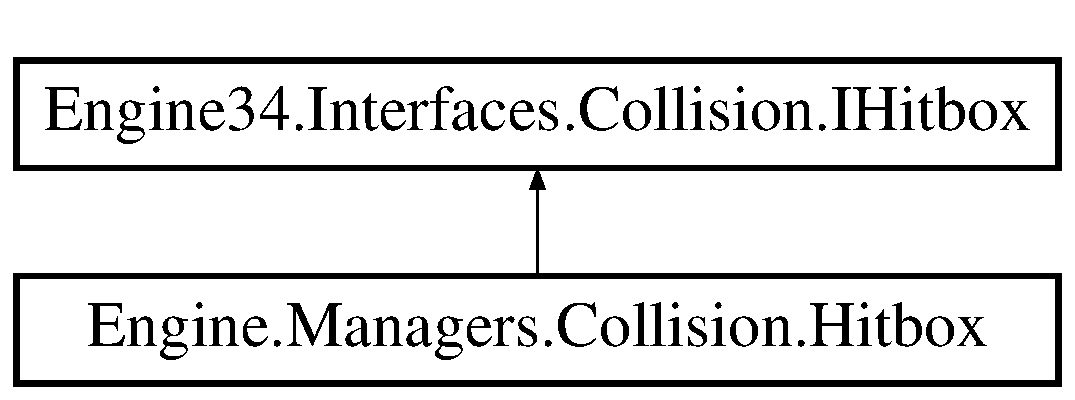
\includegraphics[height=2.000000cm]{d1/d7e/a00434}
\end{center}
\end{figure}
\subsection*{Public Member Functions}
\begin{DoxyCompactItemize}
\item 
void \hyperlink{a00434_acd7cc791467a53026ad0657a13265f1e}{create\+Matrix} ()
\item 
Vector2 \hyperlink{a00434_a88740a6f4bc38fab5c8a58ca80f70aa7}{create\+Rotation} (Vector2 \+\_\+point)
\item 
void \hyperlink{a00434_a94297321cbc20a7cb6a98cf38b735a5b}{Create\+Edges} ()
\item 
void \hyperlink{a00434_ae50d408a05951b1e4db24bb468860103}{Update\+Point} (Vector2 velocity)
\item 
Vector2 \hyperlink{a00434_a5028f79a4e2537e578c528c932dee948}{centre\+Point} ()
\item 
void \hyperlink{a00434_a50eba986052aa1f6ac4b49426ab31042}{Update} ()
\end{DoxyCompactItemize}
\subsection*{Properties}
\begin{DoxyCompactItemize}
\item 
List$<$ Vector2 $>$ \hyperlink{a00434_adf3ddbfb39ee755496a5b66cbc6dc498}{Points}\hspace{0.3cm}{\ttfamily  \mbox{[}get, set\mbox{]}}
\item 
List$<$ Vector2 $>$ \hyperlink{a00434_a21277c9cf2693302c836948c683692e9}{Edges}\hspace{0.3cm}{\ttfamily  \mbox{[}get, set\mbox{]}}
\item 
Vector2 \hyperlink{a00434_a7b1549f95caadf4aa47757631724a33a}{Velocity}\hspace{0.3cm}{\ttfamily  \mbox{[}get, set\mbox{]}}
\item 
\hyperlink{a00446}{I\+Mind} \hyperlink{a00434_abbe120cf43c047de61541acb812a1e7b}{Mind}\hspace{0.3cm}{\ttfamily  \mbox{[}get, set\mbox{]}}
\item 
Vector2 \hyperlink{a00434_afa4a2607d8572fda7c7a8a8b120a3320}{Centre}\hspace{0.3cm}{\ttfamily  \mbox{[}get, set\mbox{]}}
\end{DoxyCompactItemize}


\subsection{Detailed Description}
I\+N\+T\+E\+R\+F\+A\+CE\+: The interface for all hitboxes used for S\+AT \hyperlink{a00256}{Collision} 



\subsection{Member Function Documentation}
\mbox{\Hypertarget{a00434_a5028f79a4e2537e578c528c932dee948}\label{a00434_a5028f79a4e2537e578c528c932dee948}} 
\index{Engine34\+::\+Interfaces\+::\+Collision\+::\+I\+Hitbox@{Engine34\+::\+Interfaces\+::\+Collision\+::\+I\+Hitbox}!centre\+Point@{centre\+Point}}
\index{centre\+Point@{centre\+Point}!Engine34\+::\+Interfaces\+::\+Collision\+::\+I\+Hitbox@{Engine34\+::\+Interfaces\+::\+Collision\+::\+I\+Hitbox}}
\subsubsection{\texorpdfstring{centre\+Point()}{centrePoint()}}
{\footnotesize\ttfamily Vector2 Engine34.\+Interfaces.\+Collision.\+I\+Hitbox.\+centre\+Point (\begin{DoxyParamCaption}{ }\end{DoxyParamCaption})}



Implemented in \hyperlink{a00506_ad129f58518e4fedffc47433af729b3bf}{Engine.\+Managers.\+Collision.\+Hitbox}.

\mbox{\Hypertarget{a00434_a94297321cbc20a7cb6a98cf38b735a5b}\label{a00434_a94297321cbc20a7cb6a98cf38b735a5b}} 
\index{Engine34\+::\+Interfaces\+::\+Collision\+::\+I\+Hitbox@{Engine34\+::\+Interfaces\+::\+Collision\+::\+I\+Hitbox}!Create\+Edges@{Create\+Edges}}
\index{Create\+Edges@{Create\+Edges}!Engine34\+::\+Interfaces\+::\+Collision\+::\+I\+Hitbox@{Engine34\+::\+Interfaces\+::\+Collision\+::\+I\+Hitbox}}
\subsubsection{\texorpdfstring{Create\+Edges()}{CreateEdges()}}
{\footnotesize\ttfamily void Engine34.\+Interfaces.\+Collision.\+I\+Hitbox.\+Create\+Edges (\begin{DoxyParamCaption}{ }\end{DoxyParamCaption})}



Implemented in \hyperlink{a00506_a6bc6facadaf82a8c49979e35f0c8b132}{Engine.\+Managers.\+Collision.\+Hitbox}.

\mbox{\Hypertarget{a00434_acd7cc791467a53026ad0657a13265f1e}\label{a00434_acd7cc791467a53026ad0657a13265f1e}} 
\index{Engine34\+::\+Interfaces\+::\+Collision\+::\+I\+Hitbox@{Engine34\+::\+Interfaces\+::\+Collision\+::\+I\+Hitbox}!create\+Matrix@{create\+Matrix}}
\index{create\+Matrix@{create\+Matrix}!Engine34\+::\+Interfaces\+::\+Collision\+::\+I\+Hitbox@{Engine34\+::\+Interfaces\+::\+Collision\+::\+I\+Hitbox}}
\subsubsection{\texorpdfstring{create\+Matrix()}{createMatrix()}}
{\footnotesize\ttfamily void Engine34.\+Interfaces.\+Collision.\+I\+Hitbox.\+create\+Matrix (\begin{DoxyParamCaption}{ }\end{DoxyParamCaption})}



Implemented in \hyperlink{a00506_ab91473c67469cf0be5069c1ca9a2d6fb}{Engine.\+Managers.\+Collision.\+Hitbox}.

\mbox{\Hypertarget{a00434_a88740a6f4bc38fab5c8a58ca80f70aa7}\label{a00434_a88740a6f4bc38fab5c8a58ca80f70aa7}} 
\index{Engine34\+::\+Interfaces\+::\+Collision\+::\+I\+Hitbox@{Engine34\+::\+Interfaces\+::\+Collision\+::\+I\+Hitbox}!create\+Rotation@{create\+Rotation}}
\index{create\+Rotation@{create\+Rotation}!Engine34\+::\+Interfaces\+::\+Collision\+::\+I\+Hitbox@{Engine34\+::\+Interfaces\+::\+Collision\+::\+I\+Hitbox}}
\subsubsection{\texorpdfstring{create\+Rotation()}{createRotation()}}
{\footnotesize\ttfamily Vector2 Engine34.\+Interfaces.\+Collision.\+I\+Hitbox.\+create\+Rotation (\begin{DoxyParamCaption}\item[{Vector2}]{\+\_\+point }\end{DoxyParamCaption})}



Implemented in \hyperlink{a00506_ae78ae27deafc11bf87c1396c504ce621}{Engine.\+Managers.\+Collision.\+Hitbox}.

\mbox{\Hypertarget{a00434_a50eba986052aa1f6ac4b49426ab31042}\label{a00434_a50eba986052aa1f6ac4b49426ab31042}} 
\index{Engine34\+::\+Interfaces\+::\+Collision\+::\+I\+Hitbox@{Engine34\+::\+Interfaces\+::\+Collision\+::\+I\+Hitbox}!Update@{Update}}
\index{Update@{Update}!Engine34\+::\+Interfaces\+::\+Collision\+::\+I\+Hitbox@{Engine34\+::\+Interfaces\+::\+Collision\+::\+I\+Hitbox}}
\subsubsection{\texorpdfstring{Update()}{Update()}}
{\footnotesize\ttfamily void Engine34.\+Interfaces.\+Collision.\+I\+Hitbox.\+Update (\begin{DoxyParamCaption}{ }\end{DoxyParamCaption})}



Implemented in \hyperlink{a00506_a987b7fd544e03a9e43e38cc2df785d1d}{Engine.\+Managers.\+Collision.\+Hitbox}.

\mbox{\Hypertarget{a00434_ae50d408a05951b1e4db24bb468860103}\label{a00434_ae50d408a05951b1e4db24bb468860103}} 
\index{Engine34\+::\+Interfaces\+::\+Collision\+::\+I\+Hitbox@{Engine34\+::\+Interfaces\+::\+Collision\+::\+I\+Hitbox}!Update\+Point@{Update\+Point}}
\index{Update\+Point@{Update\+Point}!Engine34\+::\+Interfaces\+::\+Collision\+::\+I\+Hitbox@{Engine34\+::\+Interfaces\+::\+Collision\+::\+I\+Hitbox}}
\subsubsection{\texorpdfstring{Update\+Point()}{UpdatePoint()}}
{\footnotesize\ttfamily void Engine34.\+Interfaces.\+Collision.\+I\+Hitbox.\+Update\+Point (\begin{DoxyParamCaption}\item[{Vector2}]{velocity }\end{DoxyParamCaption})}



Implemented in \hyperlink{a00506_ab5cba73c16189f63616a91cf19f00562}{Engine.\+Managers.\+Collision.\+Hitbox}.



\subsection{Property Documentation}
\mbox{\Hypertarget{a00434_afa4a2607d8572fda7c7a8a8b120a3320}\label{a00434_afa4a2607d8572fda7c7a8a8b120a3320}} 
\index{Engine34\+::\+Interfaces\+::\+Collision\+::\+I\+Hitbox@{Engine34\+::\+Interfaces\+::\+Collision\+::\+I\+Hitbox}!Centre@{Centre}}
\index{Centre@{Centre}!Engine34\+::\+Interfaces\+::\+Collision\+::\+I\+Hitbox@{Engine34\+::\+Interfaces\+::\+Collision\+::\+I\+Hitbox}}
\subsubsection{\texorpdfstring{Centre}{Centre}}
{\footnotesize\ttfamily Vector2 Engine34.\+Interfaces.\+Collision.\+I\+Hitbox.\+Centre\hspace{0.3cm}{\ttfamily [get]}, {\ttfamily [set]}}

\mbox{\Hypertarget{a00434_a21277c9cf2693302c836948c683692e9}\label{a00434_a21277c9cf2693302c836948c683692e9}} 
\index{Engine34\+::\+Interfaces\+::\+Collision\+::\+I\+Hitbox@{Engine34\+::\+Interfaces\+::\+Collision\+::\+I\+Hitbox}!Edges@{Edges}}
\index{Edges@{Edges}!Engine34\+::\+Interfaces\+::\+Collision\+::\+I\+Hitbox@{Engine34\+::\+Interfaces\+::\+Collision\+::\+I\+Hitbox}}
\subsubsection{\texorpdfstring{Edges}{Edges}}
{\footnotesize\ttfamily List$<$Vector2$>$ Engine34.\+Interfaces.\+Collision.\+I\+Hitbox.\+Edges\hspace{0.3cm}{\ttfamily [get]}, {\ttfamily [set]}}

\mbox{\Hypertarget{a00434_abbe120cf43c047de61541acb812a1e7b}\label{a00434_abbe120cf43c047de61541acb812a1e7b}} 
\index{Engine34\+::\+Interfaces\+::\+Collision\+::\+I\+Hitbox@{Engine34\+::\+Interfaces\+::\+Collision\+::\+I\+Hitbox}!Mind@{Mind}}
\index{Mind@{Mind}!Engine34\+::\+Interfaces\+::\+Collision\+::\+I\+Hitbox@{Engine34\+::\+Interfaces\+::\+Collision\+::\+I\+Hitbox}}
\subsubsection{\texorpdfstring{Mind}{Mind}}
{\footnotesize\ttfamily \hyperlink{a00446}{I\+Mind} Engine34.\+Interfaces.\+Collision.\+I\+Hitbox.\+Mind\hspace{0.3cm}{\ttfamily [get]}, {\ttfamily [set]}}

\mbox{\Hypertarget{a00434_adf3ddbfb39ee755496a5b66cbc6dc498}\label{a00434_adf3ddbfb39ee755496a5b66cbc6dc498}} 
\index{Engine34\+::\+Interfaces\+::\+Collision\+::\+I\+Hitbox@{Engine34\+::\+Interfaces\+::\+Collision\+::\+I\+Hitbox}!Points@{Points}}
\index{Points@{Points}!Engine34\+::\+Interfaces\+::\+Collision\+::\+I\+Hitbox@{Engine34\+::\+Interfaces\+::\+Collision\+::\+I\+Hitbox}}
\subsubsection{\texorpdfstring{Points}{Points}}
{\footnotesize\ttfamily List$<$Vector2$>$ Engine34.\+Interfaces.\+Collision.\+I\+Hitbox.\+Points\hspace{0.3cm}{\ttfamily [get]}, {\ttfamily [set]}}

\mbox{\Hypertarget{a00434_a7b1549f95caadf4aa47757631724a33a}\label{a00434_a7b1549f95caadf4aa47757631724a33a}} 
\index{Engine34\+::\+Interfaces\+::\+Collision\+::\+I\+Hitbox@{Engine34\+::\+Interfaces\+::\+Collision\+::\+I\+Hitbox}!Velocity@{Velocity}}
\index{Velocity@{Velocity}!Engine34\+::\+Interfaces\+::\+Collision\+::\+I\+Hitbox@{Engine34\+::\+Interfaces\+::\+Collision\+::\+I\+Hitbox}}
\subsubsection{\texorpdfstring{Velocity}{Velocity}}
{\footnotesize\ttfamily Vector2 Engine34.\+Interfaces.\+Collision.\+I\+Hitbox.\+Velocity\hspace{0.3cm}{\ttfamily [get]}, {\ttfamily [set]}}



The documentation for this interface was generated from the following file\+:\begin{DoxyCompactItemize}
\item 
\hyperlink{a00107}{I\+Hitbox.\+cs}\end{DoxyCompactItemize}

\hypertarget{a00450}{}\section{Engine.\+Interfaces.\+Input\+Manager.\+I\+Input\+Manager Interface Reference}
\label{a00450}\index{Engine.\+Interfaces.\+Input\+Manager.\+I\+Input\+Manager@{Engine.\+Interfaces.\+Input\+Manager.\+I\+Input\+Manager}}


I\+N\+T\+E\+R\+F\+A\+CE\+: An interface which declares the implementation that the input manager must contain. The input manager is used to check for what keys are pressed and held on a keyboard.  


Inheritance diagram for Engine.\+Interfaces.\+Input\+Manager.\+I\+Input\+Manager\+:\begin{figure}[H]
\begin{center}
\leavevmode
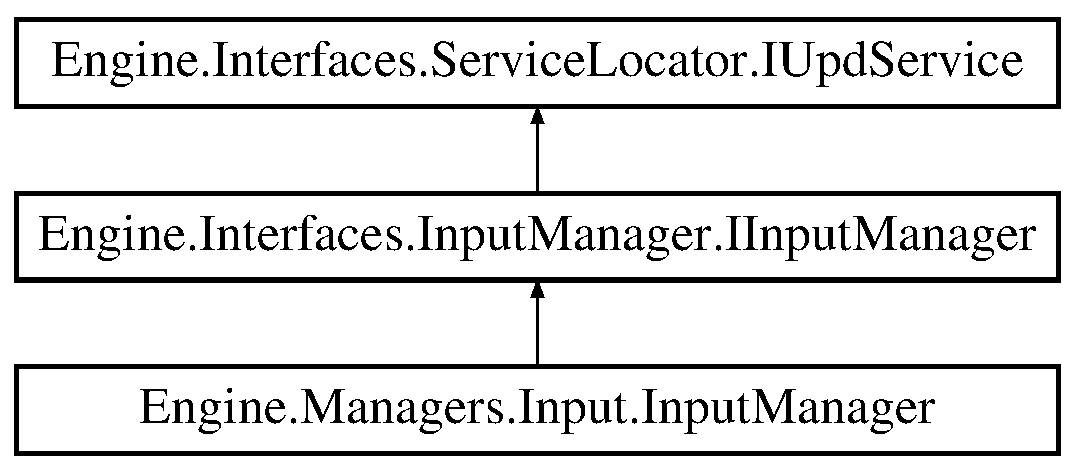
\includegraphics[height=3.000000cm]{de/df4/a00450}
\end{center}
\end{figure}
\subsection*{Public Member Functions}
\begin{DoxyCompactItemize}
\item 
void \hyperlink{a00450_a43c99a0052fd196583700113cd0bdf9f}{Update} (Game\+Time game\+Time)
\begin{DoxyCompactList}\small\item\em M\+E\+T\+H\+OD\+: Update loop which is cycled through every frame \end{DoxyCompactList}\item 
bool \hyperlink{a00450_ab31bc2c7a5da56dc4a46ac378fde0590}{Check\+Key\+Pressed} (Keys k)
\begin{DoxyCompactList}\small\item\em M\+E\+T\+H\+OD\+: returns true if when a key is pressed \end{DoxyCompactList}\item 
bool \hyperlink{a00450_a661496081120efdcd653693977f36fd9}{Check\+Held\+Down} (Keys k)
\begin{DoxyCompactList}\small\item\em M\+E\+T\+H\+OD\+: returns true when a key is held down \end{DoxyCompactList}\end{DoxyCompactItemize}


\subsection{Detailed Description}
I\+N\+T\+E\+R\+F\+A\+CE\+: An interface which declares the implementation that the input manager must contain. The input manager is used to check for what keys are pressed and held on a keyboard. 



\subsection{Member Function Documentation}
\mbox{\Hypertarget{a00450_a661496081120efdcd653693977f36fd9}\label{a00450_a661496081120efdcd653693977f36fd9}} 
\index{Engine\+::\+Interfaces\+::\+Input\+Manager\+::\+I\+Input\+Manager@{Engine\+::\+Interfaces\+::\+Input\+Manager\+::\+I\+Input\+Manager}!Check\+Held\+Down@{Check\+Held\+Down}}
\index{Check\+Held\+Down@{Check\+Held\+Down}!Engine\+::\+Interfaces\+::\+Input\+Manager\+::\+I\+Input\+Manager@{Engine\+::\+Interfaces\+::\+Input\+Manager\+::\+I\+Input\+Manager}}
\subsubsection{\texorpdfstring{Check\+Held\+Down()}{CheckHeldDown()}}
{\footnotesize\ttfamily bool Engine.\+Interfaces.\+Input\+Manager.\+I\+Input\+Manager.\+Check\+Held\+Down (\begin{DoxyParamCaption}\item[{Keys}]{k }\end{DoxyParamCaption})}



M\+E\+T\+H\+OD\+: returns true when a key is held down 


\begin{DoxyParams}{Parameters}
{\em k} & the key to be checked\\
\hline
\end{DoxyParams}
\begin{DoxyReturn}{Returns}
a bool on whether the key has been held down for more than one frame
\end{DoxyReturn}


Implemented in \hyperlink{a00522_a40428e54a6265c8e18c51489321b1d4c}{Engine.\+Managers.\+Input.\+Input\+Manager}.

\mbox{\Hypertarget{a00450_ab31bc2c7a5da56dc4a46ac378fde0590}\label{a00450_ab31bc2c7a5da56dc4a46ac378fde0590}} 
\index{Engine\+::\+Interfaces\+::\+Input\+Manager\+::\+I\+Input\+Manager@{Engine\+::\+Interfaces\+::\+Input\+Manager\+::\+I\+Input\+Manager}!Check\+Key\+Pressed@{Check\+Key\+Pressed}}
\index{Check\+Key\+Pressed@{Check\+Key\+Pressed}!Engine\+::\+Interfaces\+::\+Input\+Manager\+::\+I\+Input\+Manager@{Engine\+::\+Interfaces\+::\+Input\+Manager\+::\+I\+Input\+Manager}}
\subsubsection{\texorpdfstring{Check\+Key\+Pressed()}{CheckKeyPressed()}}
{\footnotesize\ttfamily bool Engine.\+Interfaces.\+Input\+Manager.\+I\+Input\+Manager.\+Check\+Key\+Pressed (\begin{DoxyParamCaption}\item[{Keys}]{k }\end{DoxyParamCaption})}



M\+E\+T\+H\+OD\+: returns true if when a key is pressed 


\begin{DoxyParams}{Parameters}
{\em k} & A key to be checked\\
\hline
\end{DoxyParams}
\begin{DoxyReturn}{Returns}
a bool whether the key is pressed or not
\end{DoxyReturn}


Implemented in \hyperlink{a00522_aeb5c9f3f44ec0f9468cf3ec6801b9b24}{Engine.\+Managers.\+Input.\+Input\+Manager}.

\mbox{\Hypertarget{a00450_a43c99a0052fd196583700113cd0bdf9f}\label{a00450_a43c99a0052fd196583700113cd0bdf9f}} 
\index{Engine\+::\+Interfaces\+::\+Input\+Manager\+::\+I\+Input\+Manager@{Engine\+::\+Interfaces\+::\+Input\+Manager\+::\+I\+Input\+Manager}!Update@{Update}}
\index{Update@{Update}!Engine\+::\+Interfaces\+::\+Input\+Manager\+::\+I\+Input\+Manager@{Engine\+::\+Interfaces\+::\+Input\+Manager\+::\+I\+Input\+Manager}}
\subsubsection{\texorpdfstring{Update()}{Update()}}
{\footnotesize\ttfamily void Engine.\+Interfaces.\+Input\+Manager.\+I\+Input\+Manager.\+Update (\begin{DoxyParamCaption}\item[{Game\+Time}]{game\+Time }\end{DoxyParamCaption})}



M\+E\+T\+H\+OD\+: Update loop which is cycled through every frame 


\begin{DoxyParams}{Parameters}
{\em game\+Time} & the Monogame Game\+Time\\
\hline
\end{DoxyParams}


Implements \hyperlink{a00478_a387fce2a5440a4dc63f8d72772ecbdaa}{Engine.\+Interfaces.\+Service\+Locator.\+I\+Upd\+Service}.



Implemented in \hyperlink{a00522_a7b0666f02640f9234e290938c4474e26}{Engine.\+Managers.\+Input.\+Input\+Manager}.



The documentation for this interface was generated from the following file\+:\begin{DoxyCompactItemize}
\item 
\hyperlink{a00119}{I\+Input\+Manager.\+cs}\end{DoxyCompactItemize}

\hypertarget{a00446}{}\section{Engine.\+Interfaces.\+Entities.\+I\+Mind Interface Reference}
\label{a00446}\index{Engine.\+Interfaces.\+Entities.\+I\+Mind@{Engine.\+Interfaces.\+Entities.\+I\+Mind}}


I\+N\+T\+E\+R\+F\+A\+CE\+: An interface that provides Implementation for any object that is a mind which controls the behaviour of an entity.  


Inheritance diagram for Engine.\+Interfaces.\+Entities.\+I\+Mind\+:\begin{figure}[H]
\begin{center}
\leavevmode
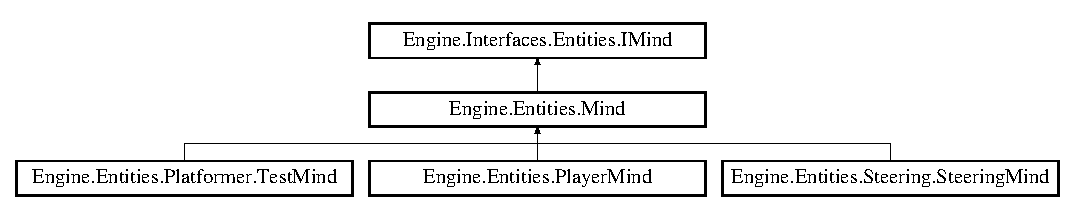
\includegraphics[height=2.403433cm]{d3/def/a00446}
\end{center}
\end{figure}
\subsection*{Public Member Functions}
\begin{DoxyCompactItemize}
\item 
void \hyperlink{a00446_a21a0486019d7c7b665fdf483626323f3}{Update} (Game\+Time game\+Time)
\begin{DoxyCompactList}\small\item\em M\+E\+T\+H\+OD\+: Update, is run every frame and is the main loop for any mind. \end{DoxyCompactList}\item 
void \hyperlink{a00446_a6f51a819769ba43f5f1702563293aacd}{Initialize} (Vector2 \hyperlink{a00446_ad1af5071b566a62b9e64aad821da9f21}{Position}, string t)
\begin{DoxyCompactList}\small\item\em M\+E\+T\+H\+OD\+: Initialise the position and texture \end{DoxyCompactList}\item 
void \hyperlink{a00446_a421d8eb0a0accda3320144fbfe33ea8c}{Initialize} (Vector2 \hyperlink{a00446_ad1af5071b566a62b9e64aad821da9f21}{Position})
\begin{DoxyCompactList}\small\item\em M\+E\+T\+H\+OD\+: Initialise just the position in case a texture has already been set. \end{DoxyCompactList}\item 
void \hyperlink{a00446_a142493645e36a3e14c7d3c59793c4d3c}{Unload} ()
\begin{DoxyCompactList}\small\item\em M\+E\+T\+H\+OD\+: Unload the mind and send it to the garbage collector. \end{DoxyCompactList}\item 
\hyperlink{a00438}{I\+Entity} \hyperlink{a00446_af7c7cac5148930a12a85ec64412ac6f2}{get\+Entity} ()
\begin{DoxyCompactList}\small\item\em M\+E\+T\+H\+OD\+: Get the entity which a mind controls. \end{DoxyCompactList}\item 
\hyperlink{a00426}{I\+Collidable} \hyperlink{a00446_a3cbff0e85b710a4c8737254ed9ca7b30}{get\+Collidable} ()
\begin{DoxyCompactList}\small\item\em M\+E\+T\+H\+OD\+: Return an object that will be calculated for collision \end{DoxyCompactList}\item 
void \hyperlink{a00446_a9d8370ad6e1b2a07760d3554b1e179fd}{Link} (\hyperlink{a00438}{I\+Entity} e)
\begin{DoxyCompactList}\small\item\em M\+E\+T\+H\+OD\+: Link the mind to an entity. \end{DoxyCompactList}\end{DoxyCompactItemize}
\subsection*{Properties}
\begin{DoxyCompactItemize}
\item 
bool \hyperlink{a00446_a50008fc232397651429a06699310ef6f}{Active}\hspace{0.3cm}{\ttfamily  \mbox{[}get, set\mbox{]}}
\begin{DoxyCompactList}\small\item\em G\+ET\+: S\+ET\+: A bool for whether the mind is currently attached to an Entity \end{DoxyCompactList}\item 
Vector2 \hyperlink{a00446_a662544c982afdebf739a9a0eaa9b7a80}{Velocity}\hspace{0.3cm}{\ttfamily  \mbox{[}get, set\mbox{]}}
\begin{DoxyCompactList}\small\item\em G\+ET\+: S\+ET\+: The velocity of the mind \end{DoxyCompactList}\item 
Vector2 \hyperlink{a00446_ad1af5071b566a62b9e64aad821da9f21}{Position}\hspace{0.3cm}{\ttfamily  \mbox{[}get, set\mbox{]}}
\begin{DoxyCompactList}\small\item\em G\+ET\+: S\+ET\+: The position of the mind. \end{DoxyCompactList}\item 
int \hyperlink{a00446_a33ec6f3f0e9f14bdcab38fd0f28148d1}{Unique\+ID}\hspace{0.3cm}{\ttfamily  \mbox{[}get\mbox{]}}
\begin{DoxyCompactList}\small\item\em G\+ET\+: The unique ID for the mind \end{DoxyCompactList}\end{DoxyCompactItemize}


\subsection{Detailed Description}
I\+N\+T\+E\+R\+F\+A\+CE\+: An interface that provides Implementation for any object that is a mind which controls the behaviour of an entity. 



\subsection{Member Function Documentation}
\mbox{\Hypertarget{a00446_a3cbff0e85b710a4c8737254ed9ca7b30}\label{a00446_a3cbff0e85b710a4c8737254ed9ca7b30}} 
\index{Engine\+::\+Interfaces\+::\+Entities\+::\+I\+Mind@{Engine\+::\+Interfaces\+::\+Entities\+::\+I\+Mind}!get\+Collidable@{get\+Collidable}}
\index{get\+Collidable@{get\+Collidable}!Engine\+::\+Interfaces\+::\+Entities\+::\+I\+Mind@{Engine\+::\+Interfaces\+::\+Entities\+::\+I\+Mind}}
\subsubsection{\texorpdfstring{get\+Collidable()}{getCollidable()}}
{\footnotesize\ttfamily \hyperlink{a00426}{I\+Collidable} Engine.\+Interfaces.\+Entities.\+I\+Mind.\+get\+Collidable (\begin{DoxyParamCaption}{ }\end{DoxyParamCaption})}



M\+E\+T\+H\+OD\+: Return an object that will be calculated for collision 

\begin{DoxyReturn}{Returns}
An I\+Collidable of the current object
\end{DoxyReturn}


Implemented in \hyperlink{a00318_aa36d6fcb8d80f1398855cea671ce1078}{Engine.\+Entities.\+Mind}.

\mbox{\Hypertarget{a00446_af7c7cac5148930a12a85ec64412ac6f2}\label{a00446_af7c7cac5148930a12a85ec64412ac6f2}} 
\index{Engine\+::\+Interfaces\+::\+Entities\+::\+I\+Mind@{Engine\+::\+Interfaces\+::\+Entities\+::\+I\+Mind}!get\+Entity@{get\+Entity}}
\index{get\+Entity@{get\+Entity}!Engine\+::\+Interfaces\+::\+Entities\+::\+I\+Mind@{Engine\+::\+Interfaces\+::\+Entities\+::\+I\+Mind}}
\subsubsection{\texorpdfstring{get\+Entity()}{getEntity()}}
{\footnotesize\ttfamily \hyperlink{a00438}{I\+Entity} Engine.\+Interfaces.\+Entities.\+I\+Mind.\+get\+Entity (\begin{DoxyParamCaption}{ }\end{DoxyParamCaption})}



M\+E\+T\+H\+OD\+: Get the entity which a mind controls. 

\begin{DoxyReturn}{Returns}
The I\+E\+Ntity this mind controls
\end{DoxyReturn}


Implemented in \hyperlink{a00318_a9585d4438e12299a42aaed4ee6fb88b6}{Engine.\+Entities.\+Mind}.

\mbox{\Hypertarget{a00446_a6f51a819769ba43f5f1702563293aacd}\label{a00446_a6f51a819769ba43f5f1702563293aacd}} 
\index{Engine\+::\+Interfaces\+::\+Entities\+::\+I\+Mind@{Engine\+::\+Interfaces\+::\+Entities\+::\+I\+Mind}!Initialize@{Initialize}}
\index{Initialize@{Initialize}!Engine\+::\+Interfaces\+::\+Entities\+::\+I\+Mind@{Engine\+::\+Interfaces\+::\+Entities\+::\+I\+Mind}}
\subsubsection{\texorpdfstring{Initialize()}{Initialize()}\hspace{0.1cm}{\footnotesize\ttfamily [1/2]}}
{\footnotesize\ttfamily void Engine.\+Interfaces.\+Entities.\+I\+Mind.\+Initialize (\begin{DoxyParamCaption}\item[{Vector2}]{Position,  }\item[{string}]{t }\end{DoxyParamCaption})}



M\+E\+T\+H\+OD\+: Initialise the position and texture 


\begin{DoxyParams}{Parameters}
{\em Position} & The position the mind will be initialised at\\
\hline
{\em t} & The string that the texture will be created from\\
\hline
\end{DoxyParams}


Implemented in \hyperlink{a00318_a386406a6250e4f7e59d0a048545ecc46}{Engine.\+Entities.\+Mind}.

\mbox{\Hypertarget{a00446_a421d8eb0a0accda3320144fbfe33ea8c}\label{a00446_a421d8eb0a0accda3320144fbfe33ea8c}} 
\index{Engine\+::\+Interfaces\+::\+Entities\+::\+I\+Mind@{Engine\+::\+Interfaces\+::\+Entities\+::\+I\+Mind}!Initialize@{Initialize}}
\index{Initialize@{Initialize}!Engine\+::\+Interfaces\+::\+Entities\+::\+I\+Mind@{Engine\+::\+Interfaces\+::\+Entities\+::\+I\+Mind}}
\subsubsection{\texorpdfstring{Initialize()}{Initialize()}\hspace{0.1cm}{\footnotesize\ttfamily [2/2]}}
{\footnotesize\ttfamily void Engine.\+Interfaces.\+Entities.\+I\+Mind.\+Initialize (\begin{DoxyParamCaption}\item[{Vector2}]{Position }\end{DoxyParamCaption})}



M\+E\+T\+H\+OD\+: Initialise just the position in case a texture has already been set. 


\begin{DoxyParams}{Parameters}
{\em Position} & The position the mind will be iniitalised at\\
\hline
\end{DoxyParams}


Implemented in \hyperlink{a00318_a353d7d2bb1035aefebf0ae3e3f1d1488}{Engine.\+Entities.\+Mind}, \hyperlink{a00346_a72922ee865087d504b1bca3fec35fb6e}{Engine.\+Entities.\+Steering.\+Steering\+Mind}, \hyperlink{a00326_a44a3007533c5d73810c4636fcfef5988}{Engine.\+Entities.\+Player\+Mind}, and \hyperlink{a00334_ae94a647a0b9c6f1d99abb61e36612ba7}{Engine.\+Entities.\+Platformer.\+Test\+Mind}.

\mbox{\Hypertarget{a00446_a9d8370ad6e1b2a07760d3554b1e179fd}\label{a00446_a9d8370ad6e1b2a07760d3554b1e179fd}} 
\index{Engine\+::\+Interfaces\+::\+Entities\+::\+I\+Mind@{Engine\+::\+Interfaces\+::\+Entities\+::\+I\+Mind}!Link@{Link}}
\index{Link@{Link}!Engine\+::\+Interfaces\+::\+Entities\+::\+I\+Mind@{Engine\+::\+Interfaces\+::\+Entities\+::\+I\+Mind}}
\subsubsection{\texorpdfstring{Link()}{Link()}}
{\footnotesize\ttfamily void Engine.\+Interfaces.\+Entities.\+I\+Mind.\+Link (\begin{DoxyParamCaption}\item[{\hyperlink{a00438}{I\+Entity}}]{e }\end{DoxyParamCaption})}



M\+E\+T\+H\+OD\+: Link the mind to an entity. 


\begin{DoxyParams}{Parameters}
{\em e} & The entity to be linked to this mind\\
\hline
\end{DoxyParams}


Implemented in \hyperlink{a00318_a3f2db3b7d2b8b68a02b56472467ffd12}{Engine.\+Entities.\+Mind}.

\mbox{\Hypertarget{a00446_a142493645e36a3e14c7d3c59793c4d3c}\label{a00446_a142493645e36a3e14c7d3c59793c4d3c}} 
\index{Engine\+::\+Interfaces\+::\+Entities\+::\+I\+Mind@{Engine\+::\+Interfaces\+::\+Entities\+::\+I\+Mind}!Unload@{Unload}}
\index{Unload@{Unload}!Engine\+::\+Interfaces\+::\+Entities\+::\+I\+Mind@{Engine\+::\+Interfaces\+::\+Entities\+::\+I\+Mind}}
\subsubsection{\texorpdfstring{Unload()}{Unload()}}
{\footnotesize\ttfamily void Engine.\+Interfaces.\+Entities.\+I\+Mind.\+Unload (\begin{DoxyParamCaption}{ }\end{DoxyParamCaption})}



M\+E\+T\+H\+OD\+: Unload the mind and send it to the garbage collector. 



Implemented in \hyperlink{a00318_a15bf25a4a74706ef37592689f43c0598}{Engine.\+Entities.\+Mind}, and \hyperlink{a00326_a80bacdc33e51129afed33f9e8bd5cd0f}{Engine.\+Entities.\+Player\+Mind}.

\mbox{\Hypertarget{a00446_a21a0486019d7c7b665fdf483626323f3}\label{a00446_a21a0486019d7c7b665fdf483626323f3}} 
\index{Engine\+::\+Interfaces\+::\+Entities\+::\+I\+Mind@{Engine\+::\+Interfaces\+::\+Entities\+::\+I\+Mind}!Update@{Update}}
\index{Update@{Update}!Engine\+::\+Interfaces\+::\+Entities\+::\+I\+Mind@{Engine\+::\+Interfaces\+::\+Entities\+::\+I\+Mind}}
\subsubsection{\texorpdfstring{Update()}{Update()}}
{\footnotesize\ttfamily void Engine.\+Interfaces.\+Entities.\+I\+Mind.\+Update (\begin{DoxyParamCaption}\item[{Game\+Time}]{game\+Time }\end{DoxyParamCaption})}



M\+E\+T\+H\+OD\+: Update, is run every frame and is the main loop for any mind. 


\begin{DoxyParams}{Parameters}
{\em game\+Time} & the Monogame Game\+Time Property\\
\hline
\end{DoxyParams}


Implemented in \hyperlink{a00318_adec6999d87accf7371de1536eac2541b}{Engine.\+Entities.\+Mind}, \hyperlink{a00346_a2e1f7ec281cfe2b7e8268a93bec59d4a}{Engine.\+Entities.\+Steering.\+Steering\+Mind}, \hyperlink{a00326_a172dca0ea26dfd821b413f7592a98084}{Engine.\+Entities.\+Player\+Mind}, and \hyperlink{a00334_a1817f5df935d637c737d510e39fd251f}{Engine.\+Entities.\+Platformer.\+Test\+Mind}.



\subsection{Property Documentation}
\mbox{\Hypertarget{a00446_a50008fc232397651429a06699310ef6f}\label{a00446_a50008fc232397651429a06699310ef6f}} 
\index{Engine\+::\+Interfaces\+::\+Entities\+::\+I\+Mind@{Engine\+::\+Interfaces\+::\+Entities\+::\+I\+Mind}!Active@{Active}}
\index{Active@{Active}!Engine\+::\+Interfaces\+::\+Entities\+::\+I\+Mind@{Engine\+::\+Interfaces\+::\+Entities\+::\+I\+Mind}}
\subsubsection{\texorpdfstring{Active}{Active}}
{\footnotesize\ttfamily bool Engine.\+Interfaces.\+Entities.\+I\+Mind.\+Active\hspace{0.3cm}{\ttfamily [get]}, {\ttfamily [set]}}



G\+ET\+: S\+ET\+: A bool for whether the mind is currently attached to an Entity 

\mbox{\Hypertarget{a00446_ad1af5071b566a62b9e64aad821da9f21}\label{a00446_ad1af5071b566a62b9e64aad821da9f21}} 
\index{Engine\+::\+Interfaces\+::\+Entities\+::\+I\+Mind@{Engine\+::\+Interfaces\+::\+Entities\+::\+I\+Mind}!Position@{Position}}
\index{Position@{Position}!Engine\+::\+Interfaces\+::\+Entities\+::\+I\+Mind@{Engine\+::\+Interfaces\+::\+Entities\+::\+I\+Mind}}
\subsubsection{\texorpdfstring{Position}{Position}}
{\footnotesize\ttfamily Vector2 Engine.\+Interfaces.\+Entities.\+I\+Mind.\+Position\hspace{0.3cm}{\ttfamily [get]}, {\ttfamily [set]}}



G\+ET\+: S\+ET\+: The position of the mind. 

\mbox{\Hypertarget{a00446_a33ec6f3f0e9f14bdcab38fd0f28148d1}\label{a00446_a33ec6f3f0e9f14bdcab38fd0f28148d1}} 
\index{Engine\+::\+Interfaces\+::\+Entities\+::\+I\+Mind@{Engine\+::\+Interfaces\+::\+Entities\+::\+I\+Mind}!Unique\+ID@{Unique\+ID}}
\index{Unique\+ID@{Unique\+ID}!Engine\+::\+Interfaces\+::\+Entities\+::\+I\+Mind@{Engine\+::\+Interfaces\+::\+Entities\+::\+I\+Mind}}
\subsubsection{\texorpdfstring{Unique\+ID}{UniqueID}}
{\footnotesize\ttfamily int Engine.\+Interfaces.\+Entities.\+I\+Mind.\+Unique\+ID\hspace{0.3cm}{\ttfamily [get]}}



G\+ET\+: The unique ID for the mind 

\mbox{\Hypertarget{a00446_a662544c982afdebf739a9a0eaa9b7a80}\label{a00446_a662544c982afdebf739a9a0eaa9b7a80}} 
\index{Engine\+::\+Interfaces\+::\+Entities\+::\+I\+Mind@{Engine\+::\+Interfaces\+::\+Entities\+::\+I\+Mind}!Velocity@{Velocity}}
\index{Velocity@{Velocity}!Engine\+::\+Interfaces\+::\+Entities\+::\+I\+Mind@{Engine\+::\+Interfaces\+::\+Entities\+::\+I\+Mind}}
\subsubsection{\texorpdfstring{Velocity}{Velocity}}
{\footnotesize\ttfamily Vector2 Engine.\+Interfaces.\+Entities.\+I\+Mind.\+Velocity\hspace{0.3cm}{\ttfamily [get]}, {\ttfamily [set]}}



G\+ET\+: S\+ET\+: The velocity of the mind 



The documentation for this interface was generated from the following file\+:\begin{DoxyCompactItemize}
\item 
\hyperlink{a00116}{I\+Mind.\+cs}\end{DoxyCompactItemize}

\hypertarget{a00522}{}\section{Engine.\+Managers.\+Input.\+Input\+Manager Class Reference}
\label{a00522}\index{Engine.\+Managers.\+Input.\+Input\+Manager@{Engine.\+Managers.\+Input.\+Input\+Manager}}


C\+L\+A\+SS\+: The manager for input. This manager is responsbile for storing an array of keys pressed down and also held down on a keyboard.  


Inheritance diagram for Engine.\+Managers.\+Input.\+Input\+Manager\+:\begin{figure}[H]
\begin{center}
\leavevmode
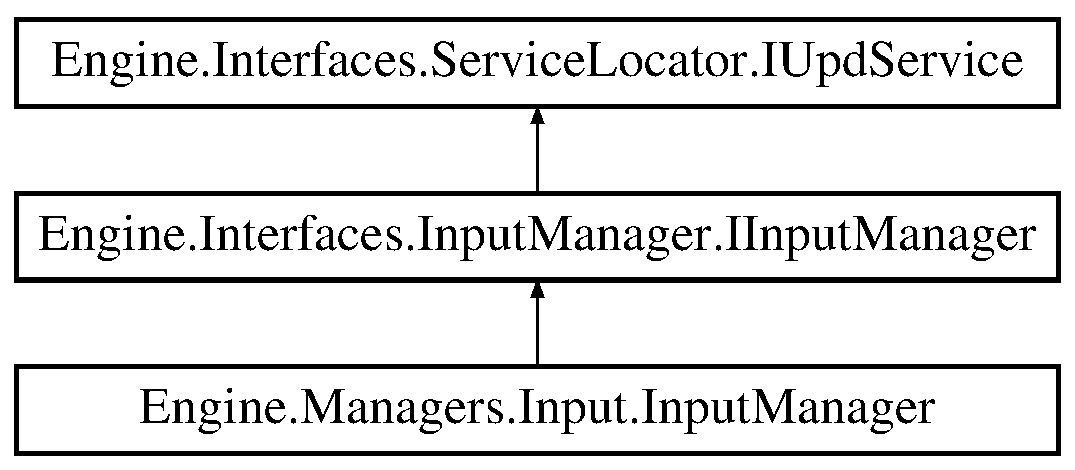
\includegraphics[height=3.000000cm]{d8/d14/a00522}
\end{center}
\end{figure}
\subsection*{Public Member Functions}
\begin{DoxyCompactItemize}
\item 
void \hyperlink{a00522_a7b0666f02640f9234e290938c4474e26}{Update} (Game\+Time game\+Time)
\begin{DoxyCompactList}\small\item\em M\+E\+T\+H\+OD\+: Update loop which is cycled through every frame \end{DoxyCompactList}\item 
bool \hyperlink{a00522_a40428e54a6265c8e18c51489321b1d4c}{Check\+Held\+Down} (Keys k)
\begin{DoxyCompactList}\small\item\em M\+E\+T\+H\+OD\+:Check if the left key is down and return true if this is the case \end{DoxyCompactList}\item 
bool \hyperlink{a00522_aeb5c9f3f44ec0f9468cf3ec6801b9b24}{Check\+Key\+Pressed} (Keys k)
\begin{DoxyCompactList}\small\item\em M\+E\+T\+H\+OD\+: check if a key has been pressed when it wasn\textquotesingle{}t in the last loop \end{DoxyCompactList}\end{DoxyCompactItemize}


\subsection{Detailed Description}
C\+L\+A\+SS\+: The manager for input. This manager is responsbile for storing an array of keys pressed down and also held down on a keyboard. 



\subsection{Member Function Documentation}
\mbox{\Hypertarget{a00522_a40428e54a6265c8e18c51489321b1d4c}\label{a00522_a40428e54a6265c8e18c51489321b1d4c}} 
\index{Engine\+::\+Managers\+::\+Input\+::\+Input\+Manager@{Engine\+::\+Managers\+::\+Input\+::\+Input\+Manager}!Check\+Held\+Down@{Check\+Held\+Down}}
\index{Check\+Held\+Down@{Check\+Held\+Down}!Engine\+::\+Managers\+::\+Input\+::\+Input\+Manager@{Engine\+::\+Managers\+::\+Input\+::\+Input\+Manager}}
\subsubsection{\texorpdfstring{Check\+Held\+Down()}{CheckHeldDown()}}
{\footnotesize\ttfamily bool Engine.\+Managers.\+Input.\+Input\+Manager.\+Check\+Held\+Down (\begin{DoxyParamCaption}\item[{Keys}]{k }\end{DoxyParamCaption})\hspace{0.3cm}{\ttfamily [inline]}}



M\+E\+T\+H\+OD\+:Check if the left key is down and return true if this is the case 


\begin{DoxyParams}{Parameters}
{\em k} & The key to be checked\\
\hline
\end{DoxyParams}
\begin{DoxyReturn}{Returns}
a bool of whether the key is held down or not
\end{DoxyReturn}


Implements \hyperlink{a00450_a661496081120efdcd653693977f36fd9}{Engine.\+Interfaces.\+Input\+Manager.\+I\+Input\+Manager}.

\mbox{\Hypertarget{a00522_aeb5c9f3f44ec0f9468cf3ec6801b9b24}\label{a00522_aeb5c9f3f44ec0f9468cf3ec6801b9b24}} 
\index{Engine\+::\+Managers\+::\+Input\+::\+Input\+Manager@{Engine\+::\+Managers\+::\+Input\+::\+Input\+Manager}!Check\+Key\+Pressed@{Check\+Key\+Pressed}}
\index{Check\+Key\+Pressed@{Check\+Key\+Pressed}!Engine\+::\+Managers\+::\+Input\+::\+Input\+Manager@{Engine\+::\+Managers\+::\+Input\+::\+Input\+Manager}}
\subsubsection{\texorpdfstring{Check\+Key\+Pressed()}{CheckKeyPressed()}}
{\footnotesize\ttfamily bool Engine.\+Managers.\+Input.\+Input\+Manager.\+Check\+Key\+Pressed (\begin{DoxyParamCaption}\item[{Keys}]{k }\end{DoxyParamCaption})\hspace{0.3cm}{\ttfamily [inline]}}



M\+E\+T\+H\+OD\+: check if a key has been pressed when it wasn\textquotesingle{}t in the last loop 


\begin{DoxyParams}{Parameters}
{\em k} & The key to be checked\\
\hline
\end{DoxyParams}
\begin{DoxyReturn}{Returns}
a bool of whether the key is pressed or not
\end{DoxyReturn}


Implements \hyperlink{a00450_ab31bc2c7a5da56dc4a46ac378fde0590}{Engine.\+Interfaces.\+Input\+Manager.\+I\+Input\+Manager}.

\mbox{\Hypertarget{a00522_a7b0666f02640f9234e290938c4474e26}\label{a00522_a7b0666f02640f9234e290938c4474e26}} 
\index{Engine\+::\+Managers\+::\+Input\+::\+Input\+Manager@{Engine\+::\+Managers\+::\+Input\+::\+Input\+Manager}!Update@{Update}}
\index{Update@{Update}!Engine\+::\+Managers\+::\+Input\+::\+Input\+Manager@{Engine\+::\+Managers\+::\+Input\+::\+Input\+Manager}}
\subsubsection{\texorpdfstring{Update()}{Update()}}
{\footnotesize\ttfamily void Engine.\+Managers.\+Input.\+Input\+Manager.\+Update (\begin{DoxyParamCaption}\item[{Game\+Time}]{game\+Time }\end{DoxyParamCaption})\hspace{0.3cm}{\ttfamily [inline]}}



M\+E\+T\+H\+OD\+: Update loop which is cycled through every frame 


\begin{DoxyParams}{Parameters}
{\em game\+Time} & the Monogame Game\+Time\\
\hline
\end{DoxyParams}


Implements \hyperlink{a00450_a43c99a0052fd196583700113cd0bdf9f}{Engine.\+Interfaces.\+Input\+Manager.\+I\+Input\+Manager}.



The documentation for this class was generated from the following file\+:\begin{DoxyCompactItemize}
\item 
\hyperlink{a00173}{Input\+Manager.\+cs}\end{DoxyCompactItemize}

\hypertarget{a00458}{}\section{Engine.\+Interfaces.\+Render.\+I\+Render\+Manager Interface Reference}
\label{a00458}\index{Engine.\+Interfaces.\+Render.\+I\+Render\+Manager@{Engine.\+Interfaces.\+Render.\+I\+Render\+Manager}}


I\+N\+T\+E\+R\+F\+A\+CE\+: This is the interface for the render manager which is responsible for all of the drawing of content in the program  


Inheritance diagram for Engine.\+Interfaces.\+Render.\+I\+Render\+Manager\+:\begin{figure}[H]
\begin{center}
\leavevmode
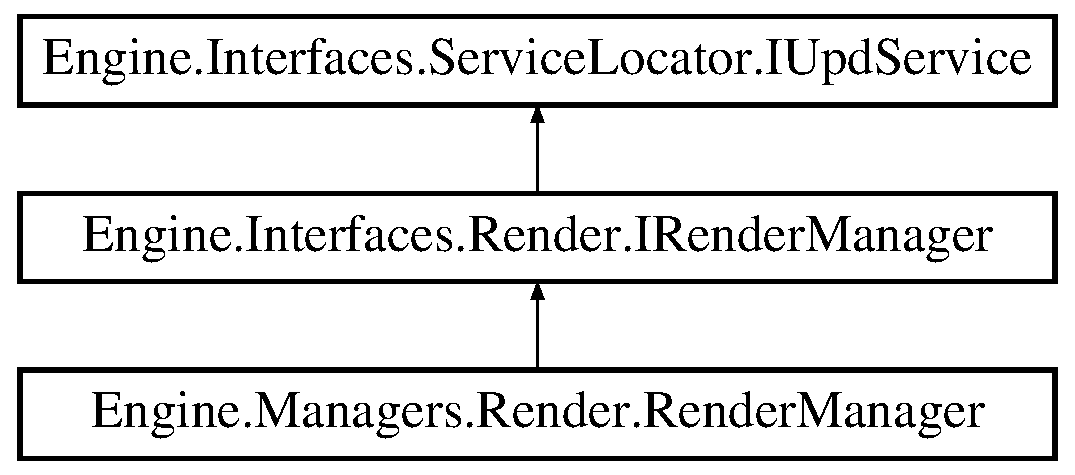
\includegraphics[height=3.000000cm]{da/d65/a00458}
\end{center}
\end{figure}
\subsection*{Public Member Functions}
\begin{DoxyCompactItemize}
\item 
void \hyperlink{a00458_ab1282efae383e9024233a2fc1eb7577b}{Initialize} ()
\begin{DoxyCompactList}\small\item\em M\+E\+T\+H\+OD\+: An initialize method that is called every time a new screen is ready to be drawn \end{DoxyCompactList}\item 
void \hyperlink{a00458_a48c8e64f7e597fdea8412057d24bcb3d}{get\+Entity\+List} ()
\begin{DoxyCompactList}\small\item\em M\+E\+T\+H\+OD\+: gets the entity list from the Entity Manager \end{DoxyCompactList}\item 
void \hyperlink{a00458_a37f1fdeb82edc4e414404d43d1c6bb51}{get\+Cam\+Entity\+List} ()
\begin{DoxyCompactList}\small\item\em M\+E\+T\+H\+OD\+: gets the entity list from the Entity Manager \end{DoxyCompactList}\item 
void \hyperlink{a00458_a3beadf9574678e62c968c8631b367348}{add\+Drawable} (\hyperlink{a00454}{I\+Drawable\+Component} d)
\begin{DoxyCompactList}\small\item\em M\+E\+T\+H\+OD\+: For items which dont wish to be drawn in regards to the cameras matrix translations (such as G\+UI) \end{DoxyCompactList}\item 
void \hyperlink{a00458_a85d74d22976a3d818b21cc856da85092}{add\+Cam\+Drawable} (\hyperlink{a00454}{I\+Drawable\+Component} d)
\begin{DoxyCompactList}\small\item\em M\+E\+T\+H\+OD\+: For Scenery/\+Entities which wish to be drawn in regards to the cameras matrix translations \end{DoxyCompactList}\item 
void \hyperlink{a00458_a5ce82555229026255b46d824edc679e8}{add\+Cam\+Draw\+Entity} (\hyperlink{a00454}{I\+Drawable\+Component} d)
\begin{DoxyCompactList}\small\item\em M\+E\+T\+H\+OD\+: For \hyperlink{a00259}{Entities} which wish to be drawn in regards to the cameras matrix translations \end{DoxyCompactList}\item 
void \hyperlink{a00458_aee587a69646dc58e02ba4430f1368bf0}{Draw\+Camera\+Related\+Artefacts} ()
\begin{DoxyCompactList}\small\item\em M\+E\+T\+H\+OD\+: Draws everything in the camera view \end{DoxyCompactList}\item 
void \hyperlink{a00458_a7879b28e310859cdebdc2c8aeaced6b3}{clear\+Temp\+Entity} ()
\begin{DoxyCompactList}\small\item\em M\+E\+T\+H\+OD\+: Clears the entities to be drawn in relation to the camera \end{DoxyCompactList}\item 
void \hyperlink{a00458_a566b23b9d0b60e2fb06107e7a6c239cb}{Draw\+Non\+Camera\+Related\+Artefacts} ()
\begin{DoxyCompactList}\small\item\em M\+E\+T\+H\+OD\+: Draws everything not related to the camera \end{DoxyCompactList}\item 
void \hyperlink{a00458_ae3d8ed9fc1406b62e04ac8336e4e40b3}{add\+String} (\hyperlink{a00598}{Game\+Text} game\+Text)
\item 
void \hyperlink{a00458_a89bf09f0f2d6144e68cd045d39f13374}{add\+Shape} (\hyperlink{a00454}{I\+Drawable\+Component} shape)
\item 
void \hyperlink{a00458_a99572d9e2280e1d7c21c002255ffe201}{Update} (Game\+Time game\+Time)
\begin{DoxyCompactList}\small\item\em M\+E\+T\+H\+OD\+: The update loop cycled through on each frame \end{DoxyCompactList}\item 
void \hyperlink{a00458_afac9eb0644db9971494332e7d179bbf9}{Draw} ()
\begin{DoxyCompactList}\small\item\em M\+E\+T\+H\+OD\+: Draws items \end{DoxyCompactList}\item 
void \hyperlink{a00458_ad9f875208c0f901d3e90facfea2acfc0}{Draw} (Texture2D texture, Rectangle rect, Color col)
\begin{DoxyCompactList}\small\item\em M\+E\+T\+H\+OD\+: Draws items \end{DoxyCompactList}\item 
void \hyperlink{a00458_aa7c35d67893f29738baab63370d16b10}{Draw\+Entities} ()
\item 
void \hyperlink{a00458_a326852d43fb14fb872d856ff2c1d6fd9}{Draw\+Components} ()
\item 
void \hyperlink{a00458_af785d8e5292f1f8f89c47d300e2c7d67}{Draw\+Shapes} ()
\item 
void \hyperlink{a00458_ace0e8fa7ce70c3437fce1298b22bf195}{Draw\+Drawables} ()
\begin{DoxyCompactList}\small\item\em M\+E\+T\+H\+OD\+: Draws every Drawable object \end{DoxyCompactList}\item 
void \hyperlink{a00458_a9239479d4d4f220b334722e48acb5bc2}{Draw\+Cam\+Drawables} ()
\begin{DoxyCompactList}\small\item\em M\+E\+T\+H\+OD\+: D\+Raws everything in relation to the camera \end{DoxyCompactList}\item 
void \hyperlink{a00458_a521ac08ccb20d1dbe58ff906fc7c42a4}{Draw\+Cam\+Draw\+Entities} ()
\begin{DoxyCompactList}\small\item\em M\+E\+T\+H\+OD\+: draws entities in relation to the camera \end{DoxyCompactList}\end{DoxyCompactItemize}
\subsection*{Properties}
\begin{DoxyCompactItemize}
\item 
Sprite\+Batch \hyperlink{a00458_a4733e89074f5ed1383e2328021fb7dd3}{sprite\+Batch}\hspace{0.3cm}{\ttfamily  \mbox{[}get, set\mbox{]}}
\end{DoxyCompactItemize}


\subsection{Detailed Description}
I\+N\+T\+E\+R\+F\+A\+CE\+: This is the interface for the render manager which is responsible for all of the drawing of content in the program 



\subsection{Member Function Documentation}
\mbox{\Hypertarget{a00458_a85d74d22976a3d818b21cc856da85092}\label{a00458_a85d74d22976a3d818b21cc856da85092}} 
\index{Engine\+::\+Interfaces\+::\+Render\+::\+I\+Render\+Manager@{Engine\+::\+Interfaces\+::\+Render\+::\+I\+Render\+Manager}!add\+Cam\+Drawable@{add\+Cam\+Drawable}}
\index{add\+Cam\+Drawable@{add\+Cam\+Drawable}!Engine\+::\+Interfaces\+::\+Render\+::\+I\+Render\+Manager@{Engine\+::\+Interfaces\+::\+Render\+::\+I\+Render\+Manager}}
\subsubsection{\texorpdfstring{add\+Cam\+Drawable()}{addCamDrawable()}}
{\footnotesize\ttfamily void Engine.\+Interfaces.\+Render.\+I\+Render\+Manager.\+add\+Cam\+Drawable (\begin{DoxyParamCaption}\item[{\hyperlink{a00454}{I\+Drawable\+Component}}]{d }\end{DoxyParamCaption})}



M\+E\+T\+H\+OD\+: For Scenery/\+Entities which wish to be drawn in regards to the cameras matrix translations 


\begin{DoxyParams}{Parameters}
{\em d} & the object to be drawn\\
\hline
\end{DoxyParams}


Implemented in \hyperlink{a00526_abe4458f6b030cffba170149d1ee63bba}{Engine.\+Managers.\+Render.\+Render\+Manager}.

\mbox{\Hypertarget{a00458_a5ce82555229026255b46d824edc679e8}\label{a00458_a5ce82555229026255b46d824edc679e8}} 
\index{Engine\+::\+Interfaces\+::\+Render\+::\+I\+Render\+Manager@{Engine\+::\+Interfaces\+::\+Render\+::\+I\+Render\+Manager}!add\+Cam\+Draw\+Entity@{add\+Cam\+Draw\+Entity}}
\index{add\+Cam\+Draw\+Entity@{add\+Cam\+Draw\+Entity}!Engine\+::\+Interfaces\+::\+Render\+::\+I\+Render\+Manager@{Engine\+::\+Interfaces\+::\+Render\+::\+I\+Render\+Manager}}
\subsubsection{\texorpdfstring{add\+Cam\+Draw\+Entity()}{addCamDrawEntity()}}
{\footnotesize\ttfamily void Engine.\+Interfaces.\+Render.\+I\+Render\+Manager.\+add\+Cam\+Draw\+Entity (\begin{DoxyParamCaption}\item[{\hyperlink{a00454}{I\+Drawable\+Component}}]{d }\end{DoxyParamCaption})}



M\+E\+T\+H\+OD\+: For \hyperlink{a00259}{Entities} which wish to be drawn in regards to the cameras matrix translations 


\begin{DoxyParams}{Parameters}
{\em d} & The object to be drawn\\
\hline
\end{DoxyParams}


Implemented in \hyperlink{a00526_a9b6bcc0390e87b334c36c1083e0af5f6}{Engine.\+Managers.\+Render.\+Render\+Manager}.

\mbox{\Hypertarget{a00458_a3beadf9574678e62c968c8631b367348}\label{a00458_a3beadf9574678e62c968c8631b367348}} 
\index{Engine\+::\+Interfaces\+::\+Render\+::\+I\+Render\+Manager@{Engine\+::\+Interfaces\+::\+Render\+::\+I\+Render\+Manager}!add\+Drawable@{add\+Drawable}}
\index{add\+Drawable@{add\+Drawable}!Engine\+::\+Interfaces\+::\+Render\+::\+I\+Render\+Manager@{Engine\+::\+Interfaces\+::\+Render\+::\+I\+Render\+Manager}}
\subsubsection{\texorpdfstring{add\+Drawable()}{addDrawable()}}
{\footnotesize\ttfamily void Engine.\+Interfaces.\+Render.\+I\+Render\+Manager.\+add\+Drawable (\begin{DoxyParamCaption}\item[{\hyperlink{a00454}{I\+Drawable\+Component}}]{d }\end{DoxyParamCaption})}



M\+E\+T\+H\+OD\+: For items which dont wish to be drawn in regards to the cameras matrix translations (such as G\+UI) 


\begin{DoxyParams}{Parameters}
{\em d} & The object to be drawn\\
\hline
\end{DoxyParams}


Implemented in \hyperlink{a00526_a6f4d9756fcf88b78263f0bc5538b1912}{Engine.\+Managers.\+Render.\+Render\+Manager}.

\mbox{\Hypertarget{a00458_a89bf09f0f2d6144e68cd045d39f13374}\label{a00458_a89bf09f0f2d6144e68cd045d39f13374}} 
\index{Engine\+::\+Interfaces\+::\+Render\+::\+I\+Render\+Manager@{Engine\+::\+Interfaces\+::\+Render\+::\+I\+Render\+Manager}!add\+Shape@{add\+Shape}}
\index{add\+Shape@{add\+Shape}!Engine\+::\+Interfaces\+::\+Render\+::\+I\+Render\+Manager@{Engine\+::\+Interfaces\+::\+Render\+::\+I\+Render\+Manager}}
\subsubsection{\texorpdfstring{add\+Shape()}{addShape()}}
{\footnotesize\ttfamily void Engine.\+Interfaces.\+Render.\+I\+Render\+Manager.\+add\+Shape (\begin{DoxyParamCaption}\item[{\hyperlink{a00454}{I\+Drawable\+Component}}]{shape }\end{DoxyParamCaption})}



Implemented in \hyperlink{a00526_a9d572b8cd8ba3c6cac622dee8d14f2a1}{Engine.\+Managers.\+Render.\+Render\+Manager}.

\mbox{\Hypertarget{a00458_ae3d8ed9fc1406b62e04ac8336e4e40b3}\label{a00458_ae3d8ed9fc1406b62e04ac8336e4e40b3}} 
\index{Engine\+::\+Interfaces\+::\+Render\+::\+I\+Render\+Manager@{Engine\+::\+Interfaces\+::\+Render\+::\+I\+Render\+Manager}!add\+String@{add\+String}}
\index{add\+String@{add\+String}!Engine\+::\+Interfaces\+::\+Render\+::\+I\+Render\+Manager@{Engine\+::\+Interfaces\+::\+Render\+::\+I\+Render\+Manager}}
\subsubsection{\texorpdfstring{add\+String()}{addString()}}
{\footnotesize\ttfamily void Engine.\+Interfaces.\+Render.\+I\+Render\+Manager.\+add\+String (\begin{DoxyParamCaption}\item[{\hyperlink{a00598}{Game\+Text}}]{game\+Text }\end{DoxyParamCaption})}



Implemented in \hyperlink{a00526_a9ce9959462da544f283ab3e531bd1edb}{Engine.\+Managers.\+Render.\+Render\+Manager}.

\mbox{\Hypertarget{a00458_a7879b28e310859cdebdc2c8aeaced6b3}\label{a00458_a7879b28e310859cdebdc2c8aeaced6b3}} 
\index{Engine\+::\+Interfaces\+::\+Render\+::\+I\+Render\+Manager@{Engine\+::\+Interfaces\+::\+Render\+::\+I\+Render\+Manager}!clear\+Temp\+Entity@{clear\+Temp\+Entity}}
\index{clear\+Temp\+Entity@{clear\+Temp\+Entity}!Engine\+::\+Interfaces\+::\+Render\+::\+I\+Render\+Manager@{Engine\+::\+Interfaces\+::\+Render\+::\+I\+Render\+Manager}}
\subsubsection{\texorpdfstring{clear\+Temp\+Entity()}{clearTempEntity()}}
{\footnotesize\ttfamily void Engine.\+Interfaces.\+Render.\+I\+Render\+Manager.\+clear\+Temp\+Entity (\begin{DoxyParamCaption}{ }\end{DoxyParamCaption})}



M\+E\+T\+H\+OD\+: Clears the entities to be drawn in relation to the camera 



Implemented in \hyperlink{a00526_af77caeb94739b508306100cdedfcbd9b}{Engine.\+Managers.\+Render.\+Render\+Manager}.

\mbox{\Hypertarget{a00458_afac9eb0644db9971494332e7d179bbf9}\label{a00458_afac9eb0644db9971494332e7d179bbf9}} 
\index{Engine\+::\+Interfaces\+::\+Render\+::\+I\+Render\+Manager@{Engine\+::\+Interfaces\+::\+Render\+::\+I\+Render\+Manager}!Draw@{Draw}}
\index{Draw@{Draw}!Engine\+::\+Interfaces\+::\+Render\+::\+I\+Render\+Manager@{Engine\+::\+Interfaces\+::\+Render\+::\+I\+Render\+Manager}}
\subsubsection{\texorpdfstring{Draw()}{Draw()}\hspace{0.1cm}{\footnotesize\ttfamily [1/2]}}
{\footnotesize\ttfamily void Engine.\+Interfaces.\+Render.\+I\+Render\+Manager.\+Draw (\begin{DoxyParamCaption}{ }\end{DoxyParamCaption})}



M\+E\+T\+H\+OD\+: Draws items 



Implemented in \hyperlink{a00526_ae9fd08da224435b71540e67f718eb7c4}{Engine.\+Managers.\+Render.\+Render\+Manager}.

\mbox{\Hypertarget{a00458_ad9f875208c0f901d3e90facfea2acfc0}\label{a00458_ad9f875208c0f901d3e90facfea2acfc0}} 
\index{Engine\+::\+Interfaces\+::\+Render\+::\+I\+Render\+Manager@{Engine\+::\+Interfaces\+::\+Render\+::\+I\+Render\+Manager}!Draw@{Draw}}
\index{Draw@{Draw}!Engine\+::\+Interfaces\+::\+Render\+::\+I\+Render\+Manager@{Engine\+::\+Interfaces\+::\+Render\+::\+I\+Render\+Manager}}
\subsubsection{\texorpdfstring{Draw()}{Draw()}\hspace{0.1cm}{\footnotesize\ttfamily [2/2]}}
{\footnotesize\ttfamily void Engine.\+Interfaces.\+Render.\+I\+Render\+Manager.\+Draw (\begin{DoxyParamCaption}\item[{Texture2D}]{texture,  }\item[{Rectangle}]{rect,  }\item[{Color}]{col }\end{DoxyParamCaption})}



M\+E\+T\+H\+OD\+: Draws items 



Implemented in \hyperlink{a00526_a5e7f7ef9bf468db27267ee1e50a34af3}{Engine.\+Managers.\+Render.\+Render\+Manager}.

\mbox{\Hypertarget{a00458_a9239479d4d4f220b334722e48acb5bc2}\label{a00458_a9239479d4d4f220b334722e48acb5bc2}} 
\index{Engine\+::\+Interfaces\+::\+Render\+::\+I\+Render\+Manager@{Engine\+::\+Interfaces\+::\+Render\+::\+I\+Render\+Manager}!Draw\+Cam\+Drawables@{Draw\+Cam\+Drawables}}
\index{Draw\+Cam\+Drawables@{Draw\+Cam\+Drawables}!Engine\+::\+Interfaces\+::\+Render\+::\+I\+Render\+Manager@{Engine\+::\+Interfaces\+::\+Render\+::\+I\+Render\+Manager}}
\subsubsection{\texorpdfstring{Draw\+Cam\+Drawables()}{DrawCamDrawables()}}
{\footnotesize\ttfamily void Engine.\+Interfaces.\+Render.\+I\+Render\+Manager.\+Draw\+Cam\+Drawables (\begin{DoxyParamCaption}{ }\end{DoxyParamCaption})}



M\+E\+T\+H\+OD\+: D\+Raws everything in relation to the camera 



Implemented in \hyperlink{a00526_adc520b6c317ed9e0d4e51fd34c22c511}{Engine.\+Managers.\+Render.\+Render\+Manager}.

\mbox{\Hypertarget{a00458_a521ac08ccb20d1dbe58ff906fc7c42a4}\label{a00458_a521ac08ccb20d1dbe58ff906fc7c42a4}} 
\index{Engine\+::\+Interfaces\+::\+Render\+::\+I\+Render\+Manager@{Engine\+::\+Interfaces\+::\+Render\+::\+I\+Render\+Manager}!Draw\+Cam\+Draw\+Entities@{Draw\+Cam\+Draw\+Entities}}
\index{Draw\+Cam\+Draw\+Entities@{Draw\+Cam\+Draw\+Entities}!Engine\+::\+Interfaces\+::\+Render\+::\+I\+Render\+Manager@{Engine\+::\+Interfaces\+::\+Render\+::\+I\+Render\+Manager}}
\subsubsection{\texorpdfstring{Draw\+Cam\+Draw\+Entities()}{DrawCamDrawEntities()}}
{\footnotesize\ttfamily void Engine.\+Interfaces.\+Render.\+I\+Render\+Manager.\+Draw\+Cam\+Draw\+Entities (\begin{DoxyParamCaption}{ }\end{DoxyParamCaption})}



M\+E\+T\+H\+OD\+: draws entities in relation to the camera 



Implemented in \hyperlink{a00526_a96510018c93924e8d5456891b28b51bb}{Engine.\+Managers.\+Render.\+Render\+Manager}.

\mbox{\Hypertarget{a00458_aee587a69646dc58e02ba4430f1368bf0}\label{a00458_aee587a69646dc58e02ba4430f1368bf0}} 
\index{Engine\+::\+Interfaces\+::\+Render\+::\+I\+Render\+Manager@{Engine\+::\+Interfaces\+::\+Render\+::\+I\+Render\+Manager}!Draw\+Camera\+Related\+Artefacts@{Draw\+Camera\+Related\+Artefacts}}
\index{Draw\+Camera\+Related\+Artefacts@{Draw\+Camera\+Related\+Artefacts}!Engine\+::\+Interfaces\+::\+Render\+::\+I\+Render\+Manager@{Engine\+::\+Interfaces\+::\+Render\+::\+I\+Render\+Manager}}
\subsubsection{\texorpdfstring{Draw\+Camera\+Related\+Artefacts()}{DrawCameraRelatedArtefacts()}}
{\footnotesize\ttfamily void Engine.\+Interfaces.\+Render.\+I\+Render\+Manager.\+Draw\+Camera\+Related\+Artefacts (\begin{DoxyParamCaption}{ }\end{DoxyParamCaption})}



M\+E\+T\+H\+OD\+: Draws everything in the camera view 



Implemented in \hyperlink{a00526_a93c2cea1133bb38a01336b3d4c6b0321}{Engine.\+Managers.\+Render.\+Render\+Manager}.

\mbox{\Hypertarget{a00458_a326852d43fb14fb872d856ff2c1d6fd9}\label{a00458_a326852d43fb14fb872d856ff2c1d6fd9}} 
\index{Engine\+::\+Interfaces\+::\+Render\+::\+I\+Render\+Manager@{Engine\+::\+Interfaces\+::\+Render\+::\+I\+Render\+Manager}!Draw\+Components@{Draw\+Components}}
\index{Draw\+Components@{Draw\+Components}!Engine\+::\+Interfaces\+::\+Render\+::\+I\+Render\+Manager@{Engine\+::\+Interfaces\+::\+Render\+::\+I\+Render\+Manager}}
\subsubsection{\texorpdfstring{Draw\+Components()}{DrawComponents()}}
{\footnotesize\ttfamily void Engine.\+Interfaces.\+Render.\+I\+Render\+Manager.\+Draw\+Components (\begin{DoxyParamCaption}{ }\end{DoxyParamCaption})}



Implemented in \hyperlink{a00526_a0df839a3a677b7595e4535716e823809}{Engine.\+Managers.\+Render.\+Render\+Manager}.

\mbox{\Hypertarget{a00458_ace0e8fa7ce70c3437fce1298b22bf195}\label{a00458_ace0e8fa7ce70c3437fce1298b22bf195}} 
\index{Engine\+::\+Interfaces\+::\+Render\+::\+I\+Render\+Manager@{Engine\+::\+Interfaces\+::\+Render\+::\+I\+Render\+Manager}!Draw\+Drawables@{Draw\+Drawables}}
\index{Draw\+Drawables@{Draw\+Drawables}!Engine\+::\+Interfaces\+::\+Render\+::\+I\+Render\+Manager@{Engine\+::\+Interfaces\+::\+Render\+::\+I\+Render\+Manager}}
\subsubsection{\texorpdfstring{Draw\+Drawables()}{DrawDrawables()}}
{\footnotesize\ttfamily void Engine.\+Interfaces.\+Render.\+I\+Render\+Manager.\+Draw\+Drawables (\begin{DoxyParamCaption}{ }\end{DoxyParamCaption})}



M\+E\+T\+H\+OD\+: Draws every Drawable object 



Implemented in \hyperlink{a00526_aa957794d6537025fb2535517bcc691cc}{Engine.\+Managers.\+Render.\+Render\+Manager}.

\mbox{\Hypertarget{a00458_aa7c35d67893f29738baab63370d16b10}\label{a00458_aa7c35d67893f29738baab63370d16b10}} 
\index{Engine\+::\+Interfaces\+::\+Render\+::\+I\+Render\+Manager@{Engine\+::\+Interfaces\+::\+Render\+::\+I\+Render\+Manager}!Draw\+Entities@{Draw\+Entities}}
\index{Draw\+Entities@{Draw\+Entities}!Engine\+::\+Interfaces\+::\+Render\+::\+I\+Render\+Manager@{Engine\+::\+Interfaces\+::\+Render\+::\+I\+Render\+Manager}}
\subsubsection{\texorpdfstring{Draw\+Entities()}{DrawEntities()}}
{\footnotesize\ttfamily void Engine.\+Interfaces.\+Render.\+I\+Render\+Manager.\+Draw\+Entities (\begin{DoxyParamCaption}{ }\end{DoxyParamCaption})}



Implemented in \hyperlink{a00526_a9eb548f058744b031b639810a16ba40d}{Engine.\+Managers.\+Render.\+Render\+Manager}.

\mbox{\Hypertarget{a00458_a566b23b9d0b60e2fb06107e7a6c239cb}\label{a00458_a566b23b9d0b60e2fb06107e7a6c239cb}} 
\index{Engine\+::\+Interfaces\+::\+Render\+::\+I\+Render\+Manager@{Engine\+::\+Interfaces\+::\+Render\+::\+I\+Render\+Manager}!Draw\+Non\+Camera\+Related\+Artefacts@{Draw\+Non\+Camera\+Related\+Artefacts}}
\index{Draw\+Non\+Camera\+Related\+Artefacts@{Draw\+Non\+Camera\+Related\+Artefacts}!Engine\+::\+Interfaces\+::\+Render\+::\+I\+Render\+Manager@{Engine\+::\+Interfaces\+::\+Render\+::\+I\+Render\+Manager}}
\subsubsection{\texorpdfstring{Draw\+Non\+Camera\+Related\+Artefacts()}{DrawNonCameraRelatedArtefacts()}}
{\footnotesize\ttfamily void Engine.\+Interfaces.\+Render.\+I\+Render\+Manager.\+Draw\+Non\+Camera\+Related\+Artefacts (\begin{DoxyParamCaption}{ }\end{DoxyParamCaption})}



M\+E\+T\+H\+OD\+: Draws everything not related to the camera 



Implemented in \hyperlink{a00526_a0dfca7db5472741f87837e7f87e90129}{Engine.\+Managers.\+Render.\+Render\+Manager}.

\mbox{\Hypertarget{a00458_af785d8e5292f1f8f89c47d300e2c7d67}\label{a00458_af785d8e5292f1f8f89c47d300e2c7d67}} 
\index{Engine\+::\+Interfaces\+::\+Render\+::\+I\+Render\+Manager@{Engine\+::\+Interfaces\+::\+Render\+::\+I\+Render\+Manager}!Draw\+Shapes@{Draw\+Shapes}}
\index{Draw\+Shapes@{Draw\+Shapes}!Engine\+::\+Interfaces\+::\+Render\+::\+I\+Render\+Manager@{Engine\+::\+Interfaces\+::\+Render\+::\+I\+Render\+Manager}}
\subsubsection{\texorpdfstring{Draw\+Shapes()}{DrawShapes()}}
{\footnotesize\ttfamily void Engine.\+Interfaces.\+Render.\+I\+Render\+Manager.\+Draw\+Shapes (\begin{DoxyParamCaption}{ }\end{DoxyParamCaption})}



Implemented in \hyperlink{a00526_af81e4faf42327afbf604c3bb4d09499a}{Engine.\+Managers.\+Render.\+Render\+Manager}.

\mbox{\Hypertarget{a00458_a37f1fdeb82edc4e414404d43d1c6bb51}\label{a00458_a37f1fdeb82edc4e414404d43d1c6bb51}} 
\index{Engine\+::\+Interfaces\+::\+Render\+::\+I\+Render\+Manager@{Engine\+::\+Interfaces\+::\+Render\+::\+I\+Render\+Manager}!get\+Cam\+Entity\+List@{get\+Cam\+Entity\+List}}
\index{get\+Cam\+Entity\+List@{get\+Cam\+Entity\+List}!Engine\+::\+Interfaces\+::\+Render\+::\+I\+Render\+Manager@{Engine\+::\+Interfaces\+::\+Render\+::\+I\+Render\+Manager}}
\subsubsection{\texorpdfstring{get\+Cam\+Entity\+List()}{getCamEntityList()}}
{\footnotesize\ttfamily void Engine.\+Interfaces.\+Render.\+I\+Render\+Manager.\+get\+Cam\+Entity\+List (\begin{DoxyParamCaption}{ }\end{DoxyParamCaption})}



M\+E\+T\+H\+OD\+: gets the entity list from the Entity Manager 



Implemented in \hyperlink{a00526_a79fb84c735ca8b863eed41f51566f554}{Engine.\+Managers.\+Render.\+Render\+Manager}.

\mbox{\Hypertarget{a00458_a48c8e64f7e597fdea8412057d24bcb3d}\label{a00458_a48c8e64f7e597fdea8412057d24bcb3d}} 
\index{Engine\+::\+Interfaces\+::\+Render\+::\+I\+Render\+Manager@{Engine\+::\+Interfaces\+::\+Render\+::\+I\+Render\+Manager}!get\+Entity\+List@{get\+Entity\+List}}
\index{get\+Entity\+List@{get\+Entity\+List}!Engine\+::\+Interfaces\+::\+Render\+::\+I\+Render\+Manager@{Engine\+::\+Interfaces\+::\+Render\+::\+I\+Render\+Manager}}
\subsubsection{\texorpdfstring{get\+Entity\+List()}{getEntityList()}}
{\footnotesize\ttfamily void Engine.\+Interfaces.\+Render.\+I\+Render\+Manager.\+get\+Entity\+List (\begin{DoxyParamCaption}{ }\end{DoxyParamCaption})}



M\+E\+T\+H\+OD\+: gets the entity list from the Entity Manager 



Implemented in \hyperlink{a00526_aeb436300e604d81ff837227e5dd11710}{Engine.\+Managers.\+Render.\+Render\+Manager}.

\mbox{\Hypertarget{a00458_ab1282efae383e9024233a2fc1eb7577b}\label{a00458_ab1282efae383e9024233a2fc1eb7577b}} 
\index{Engine\+::\+Interfaces\+::\+Render\+::\+I\+Render\+Manager@{Engine\+::\+Interfaces\+::\+Render\+::\+I\+Render\+Manager}!Initialize@{Initialize}}
\index{Initialize@{Initialize}!Engine\+::\+Interfaces\+::\+Render\+::\+I\+Render\+Manager@{Engine\+::\+Interfaces\+::\+Render\+::\+I\+Render\+Manager}}
\subsubsection{\texorpdfstring{Initialize()}{Initialize()}}
{\footnotesize\ttfamily void Engine.\+Interfaces.\+Render.\+I\+Render\+Manager.\+Initialize (\begin{DoxyParamCaption}{ }\end{DoxyParamCaption})}



M\+E\+T\+H\+OD\+: An initialize method that is called every time a new screen is ready to be drawn 



Implemented in \hyperlink{a00526_abd794ae4c12392323e9afda73e459bef}{Engine.\+Managers.\+Render.\+Render\+Manager}.

\mbox{\Hypertarget{a00458_a99572d9e2280e1d7c21c002255ffe201}\label{a00458_a99572d9e2280e1d7c21c002255ffe201}} 
\index{Engine\+::\+Interfaces\+::\+Render\+::\+I\+Render\+Manager@{Engine\+::\+Interfaces\+::\+Render\+::\+I\+Render\+Manager}!Update@{Update}}
\index{Update@{Update}!Engine\+::\+Interfaces\+::\+Render\+::\+I\+Render\+Manager@{Engine\+::\+Interfaces\+::\+Render\+::\+I\+Render\+Manager}}
\subsubsection{\texorpdfstring{Update()}{Update()}}
{\footnotesize\ttfamily void Engine.\+Interfaces.\+Render.\+I\+Render\+Manager.\+Update (\begin{DoxyParamCaption}\item[{Game\+Time}]{game\+Time }\end{DoxyParamCaption})}



M\+E\+T\+H\+OD\+: The update loop cycled through on each frame 


\begin{DoxyParams}{Parameters}
{\em game\+Time} & Monogame Game\+Time property\\
\hline
\end{DoxyParams}


Implements \hyperlink{a00478_a387fce2a5440a4dc63f8d72772ecbdaa}{Engine.\+Interfaces.\+Service\+Locator.\+I\+Upd\+Service}.



Implemented in \hyperlink{a00526_a7b63b947d986ab05b66c4c9f78ee3c20}{Engine.\+Managers.\+Render.\+Render\+Manager}.



\subsection{Property Documentation}
\mbox{\Hypertarget{a00458_a4733e89074f5ed1383e2328021fb7dd3}\label{a00458_a4733e89074f5ed1383e2328021fb7dd3}} 
\index{Engine\+::\+Interfaces\+::\+Render\+::\+I\+Render\+Manager@{Engine\+::\+Interfaces\+::\+Render\+::\+I\+Render\+Manager}!sprite\+Batch@{sprite\+Batch}}
\index{sprite\+Batch@{sprite\+Batch}!Engine\+::\+Interfaces\+::\+Render\+::\+I\+Render\+Manager@{Engine\+::\+Interfaces\+::\+Render\+::\+I\+Render\+Manager}}
\subsubsection{\texorpdfstring{sprite\+Batch}{spriteBatch}}
{\footnotesize\ttfamily Sprite\+Batch Engine.\+Interfaces.\+Render.\+I\+Render\+Manager.\+sprite\+Batch\hspace{0.3cm}{\ttfamily [get]}, {\ttfamily [set]}}



The documentation for this interface was generated from the following file\+:\begin{DoxyCompactItemize}
\item 
\hyperlink{a00125}{I\+Render\+Manager.\+cs}\end{DoxyCompactItemize}

\hypertarget{a00462}{}\section{Engine.\+Interfaces.\+Resource.\+I\+Resource\+Loader Interface Reference}
\label{a00462}\index{Engine.\+Interfaces.\+Resource.\+I\+Resource\+Loader@{Engine.\+Interfaces.\+Resource.\+I\+Resource\+Loader}}


I\+N\+T\+E\+R\+F\+A\+CE\+: Holds the implementation for the \hyperlink{a00262}{Resource} Loader which is responsible for loading and storing any external resources such as textures and sounds.  


Inheritance diagram for Engine.\+Interfaces.\+Resource.\+I\+Resource\+Loader\+:\begin{figure}[H]
\begin{center}
\leavevmode
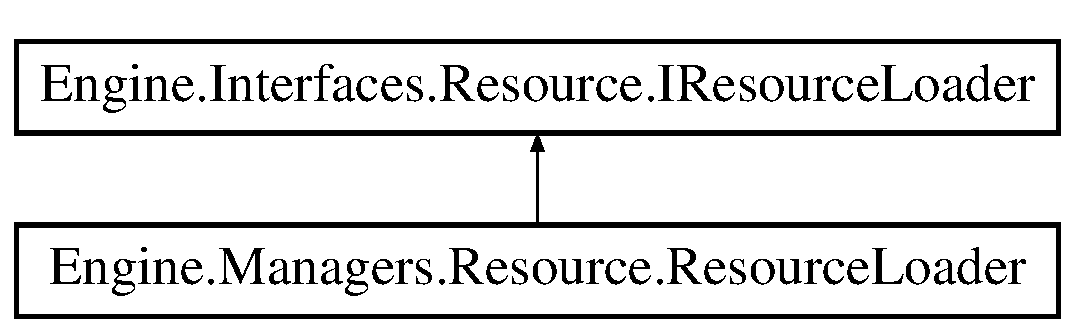
\includegraphics[height=2.000000cm]{de/dcb/a00462}
\end{center}
\end{figure}
\subsection*{Public Member Functions}
\begin{DoxyCompactItemize}
\item 
Texture2D \hyperlink{a00462_ad126b831364ad6219c3f25729c591597}{Get\+Tex} (string name)
\begin{DoxyCompactList}\small\item\em M\+E\+T\+H\+OD\+: Get a Texture from a string directory \end{DoxyCompactList}\item 
Sprite\+Font \hyperlink{a00462_abe9339a97b29bce2ba8a77504495f27d}{Get\+Font} (string name)
\begin{DoxyCompactList}\small\item\em M\+E\+T\+H\+OD\+: Get a font from a string directory \end{DoxyCompactList}\item 
Song \hyperlink{a00462_a6d962a64dc4f377bdb417598b17c53d0}{Get\+Song} (string path)
\begin{DoxyCompactList}\small\item\em M\+E\+T\+H\+OD\+: Get an audio file from a string directory \end{DoxyCompactList}\item 
void \hyperlink{a00462_ad861af436f861ea7d9c0966edfadac82}{Initialize} ()
\begin{DoxyCompactList}\small\item\em M\+E\+T\+H\+OD\+: Initialises and Loads appropriate resources \end{DoxyCompactList}\item 
bool \hyperlink{a00462_a08d51ffa3d65fd1122614e00a275cf48}{Check\+Library} (string name)
\begin{DoxyCompactList}\small\item\em M\+E\+T\+H\+OD\+: checks if a music file in the current library is valid and returns a bool \end{DoxyCompactList}\end{DoxyCompactItemize}
\subsection*{Properties}
\begin{DoxyCompactItemize}
\item 
Content\+Manager \hyperlink{a00462_a03b81447dfab7f3391b8f265dfd231c8}{Content}\hspace{0.3cm}{\ttfamily  \mbox{[}get, set\mbox{]}}
\begin{DoxyCompactList}\small\item\em G\+ET\+: S\+ET\+: The Monogame Content\+Manager \end{DoxyCompactList}\end{DoxyCompactItemize}


\subsection{Detailed Description}
I\+N\+T\+E\+R\+F\+A\+CE\+: Holds the implementation for the \hyperlink{a00262}{Resource} Loader which is responsible for loading and storing any external resources such as textures and sounds. 



\subsection{Member Function Documentation}
\mbox{\Hypertarget{a00462_a08d51ffa3d65fd1122614e00a275cf48}\label{a00462_a08d51ffa3d65fd1122614e00a275cf48}} 
\index{Engine\+::\+Interfaces\+::\+Resource\+::\+I\+Resource\+Loader@{Engine\+::\+Interfaces\+::\+Resource\+::\+I\+Resource\+Loader}!Check\+Library@{Check\+Library}}
\index{Check\+Library@{Check\+Library}!Engine\+::\+Interfaces\+::\+Resource\+::\+I\+Resource\+Loader@{Engine\+::\+Interfaces\+::\+Resource\+::\+I\+Resource\+Loader}}
\subsubsection{\texorpdfstring{Check\+Library()}{CheckLibrary()}}
{\footnotesize\ttfamily bool Engine.\+Interfaces.\+Resource.\+I\+Resource\+Loader.\+Check\+Library (\begin{DoxyParamCaption}\item[{string}]{name }\end{DoxyParamCaption})}



M\+E\+T\+H\+OD\+: checks if a music file in the current library is valid and returns a bool 


\begin{DoxyParams}{Parameters}
{\em name} & The name of the audio file to look for\\
\hline
\end{DoxyParams}
\begin{DoxyReturn}{Returns}
a boolean if the audio file exists in the queue
\end{DoxyReturn}


Implemented in \hyperlink{a00530_a939824a1d16e96b4322225a18f7a47d6}{Engine.\+Managers.\+Resource.\+Resource\+Loader}.

\mbox{\Hypertarget{a00462_abe9339a97b29bce2ba8a77504495f27d}\label{a00462_abe9339a97b29bce2ba8a77504495f27d}} 
\index{Engine\+::\+Interfaces\+::\+Resource\+::\+I\+Resource\+Loader@{Engine\+::\+Interfaces\+::\+Resource\+::\+I\+Resource\+Loader}!Get\+Font@{Get\+Font}}
\index{Get\+Font@{Get\+Font}!Engine\+::\+Interfaces\+::\+Resource\+::\+I\+Resource\+Loader@{Engine\+::\+Interfaces\+::\+Resource\+::\+I\+Resource\+Loader}}
\subsubsection{\texorpdfstring{Get\+Font()}{GetFont()}}
{\footnotesize\ttfamily Sprite\+Font Engine.\+Interfaces.\+Resource.\+I\+Resource\+Loader.\+Get\+Font (\begin{DoxyParamCaption}\item[{string}]{name }\end{DoxyParamCaption})}



M\+E\+T\+H\+OD\+: Get a font from a string directory 


\begin{DoxyParams}{Parameters}
{\em name} & The name of the font file to be loaded\\
\hline
\end{DoxyParams}
\begin{DoxyReturn}{Returns}
a Sprite\+Font of the font at the name provided
\end{DoxyReturn}


Implemented in \hyperlink{a00530_a160f06963928da598da9f9431ba65f73}{Engine.\+Managers.\+Resource.\+Resource\+Loader}.

\mbox{\Hypertarget{a00462_a6d962a64dc4f377bdb417598b17c53d0}\label{a00462_a6d962a64dc4f377bdb417598b17c53d0}} 
\index{Engine\+::\+Interfaces\+::\+Resource\+::\+I\+Resource\+Loader@{Engine\+::\+Interfaces\+::\+Resource\+::\+I\+Resource\+Loader}!Get\+Song@{Get\+Song}}
\index{Get\+Song@{Get\+Song}!Engine\+::\+Interfaces\+::\+Resource\+::\+I\+Resource\+Loader@{Engine\+::\+Interfaces\+::\+Resource\+::\+I\+Resource\+Loader}}
\subsubsection{\texorpdfstring{Get\+Song()}{GetSong()}}
{\footnotesize\ttfamily Song Engine.\+Interfaces.\+Resource.\+I\+Resource\+Loader.\+Get\+Song (\begin{DoxyParamCaption}\item[{string}]{path }\end{DoxyParamCaption})}



M\+E\+T\+H\+OD\+: Get an audio file from a string directory 


\begin{DoxyParams}{Parameters}
{\em path} & The name of the audio file to be loaded\\
\hline
\end{DoxyParams}
\begin{DoxyReturn}{Returns}
A song of the audio at the name provided
\end{DoxyReturn}


Implemented in \hyperlink{a00530_a6587452c5637a132330fb0e2f6dc4e7a}{Engine.\+Managers.\+Resource.\+Resource\+Loader}.

\mbox{\Hypertarget{a00462_ad126b831364ad6219c3f25729c591597}\label{a00462_ad126b831364ad6219c3f25729c591597}} 
\index{Engine\+::\+Interfaces\+::\+Resource\+::\+I\+Resource\+Loader@{Engine\+::\+Interfaces\+::\+Resource\+::\+I\+Resource\+Loader}!Get\+Tex@{Get\+Tex}}
\index{Get\+Tex@{Get\+Tex}!Engine\+::\+Interfaces\+::\+Resource\+::\+I\+Resource\+Loader@{Engine\+::\+Interfaces\+::\+Resource\+::\+I\+Resource\+Loader}}
\subsubsection{\texorpdfstring{Get\+Tex()}{GetTex()}}
{\footnotesize\ttfamily Texture2D Engine.\+Interfaces.\+Resource.\+I\+Resource\+Loader.\+Get\+Tex (\begin{DoxyParamCaption}\item[{string}]{name }\end{DoxyParamCaption})}



M\+E\+T\+H\+OD\+: Get a Texture from a string directory 


\begin{DoxyParams}{Parameters}
{\em name} & the name of the texture file to be loaded\\
\hline
\end{DoxyParams}
\begin{DoxyReturn}{Returns}
a Texture2D file of the image at the name provided
\end{DoxyReturn}


Implemented in \hyperlink{a00530_a841de899c3601b3d35496ee798a6e894}{Engine.\+Managers.\+Resource.\+Resource\+Loader}.

\mbox{\Hypertarget{a00462_ad861af436f861ea7d9c0966edfadac82}\label{a00462_ad861af436f861ea7d9c0966edfadac82}} 
\index{Engine\+::\+Interfaces\+::\+Resource\+::\+I\+Resource\+Loader@{Engine\+::\+Interfaces\+::\+Resource\+::\+I\+Resource\+Loader}!Initialize@{Initialize}}
\index{Initialize@{Initialize}!Engine\+::\+Interfaces\+::\+Resource\+::\+I\+Resource\+Loader@{Engine\+::\+Interfaces\+::\+Resource\+::\+I\+Resource\+Loader}}
\subsubsection{\texorpdfstring{Initialize()}{Initialize()}}
{\footnotesize\ttfamily void Engine.\+Interfaces.\+Resource.\+I\+Resource\+Loader.\+Initialize (\begin{DoxyParamCaption}{ }\end{DoxyParamCaption})}



M\+E\+T\+H\+OD\+: Initialises and Loads appropriate resources 



Implemented in \hyperlink{a00530_a77b00bda1dc37c9cabe2dbaf90655714}{Engine.\+Managers.\+Resource.\+Resource\+Loader}.



\subsection{Property Documentation}
\mbox{\Hypertarget{a00462_a03b81447dfab7f3391b8f265dfd231c8}\label{a00462_a03b81447dfab7f3391b8f265dfd231c8}} 
\index{Engine\+::\+Interfaces\+::\+Resource\+::\+I\+Resource\+Loader@{Engine\+::\+Interfaces\+::\+Resource\+::\+I\+Resource\+Loader}!Content@{Content}}
\index{Content@{Content}!Engine\+::\+Interfaces\+::\+Resource\+::\+I\+Resource\+Loader@{Engine\+::\+Interfaces\+::\+Resource\+::\+I\+Resource\+Loader}}
\subsubsection{\texorpdfstring{Content}{Content}}
{\footnotesize\ttfamily Content\+Manager Engine.\+Interfaces.\+Resource.\+I\+Resource\+Loader.\+Content\hspace{0.3cm}{\ttfamily [get]}, {\ttfamily [set]}}



G\+ET\+: S\+ET\+: The Monogame Content\+Manager 



The documentation for this interface was generated from the following file\+:\begin{DoxyCompactItemize}
\item 
\hyperlink{a00128}{I\+Resource\+Loader.\+cs}\end{DoxyCompactItemize}

\hypertarget{a00466}{}\section{Engine.\+Interfaces.\+Screen.\+I\+Screen Interface Reference}
\label{a00466}\index{Engine.\+Interfaces.\+Screen.\+I\+Screen@{Engine.\+Interfaces.\+Screen.\+I\+Screen}}


I\+N\+T\+E\+R\+F\+A\+CE\+: all screens subscribe to this interface which contains the implementation for what each screen needs To do  


Inheritance diagram for Engine.\+Interfaces.\+Screen.\+I\+Screen\+:\begin{figure}[H]
\begin{center}
\leavevmode
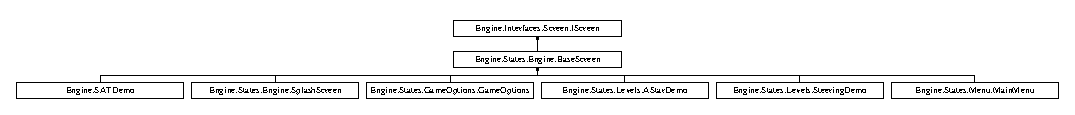
\includegraphics[height=1.098039cm]{db/d2c/a00466}
\end{center}
\end{figure}
\subsection*{Public Member Functions}
\begin{DoxyCompactItemize}
\item 
void \hyperlink{a00466_aeba867b4e4bd2f0a918b837d93a4e45a}{Unload\+Content} ()
\begin{DoxyCompactList}\small\item\em M\+E\+T\+H\+OD\+: Unloads the content of the screen \end{DoxyCompactList}\item 
void \hyperlink{a00466_ad251ad712685a0f329ad2b29bde78981}{Initialize} ()
\begin{DoxyCompactList}\small\item\em M\+E\+T\+H\+OD\+: Initialises the logic of the screen \end{DoxyCompactList}\item 
void \hyperlink{a00466_a5f59b9b12c1bf29b1db612ed52d1cfd6}{Update} (Game\+Time game\+Time)
\begin{DoxyCompactList}\small\item\em M\+E\+T\+H\+OD\+: The update loop which is cycled through each frame \end{DoxyCompactList}\item 
void \hyperlink{a00466_a0c61f739fb252fcc90b91b1358511d05}{Draw} (Sprite\+Batch sprite\+Batch)
\begin{DoxyCompactList}\small\item\em M\+E\+T\+H\+OD\+: Draws the content of the screen \end{DoxyCompactList}\item 
void \hyperlink{a00466_a67f1b5deb3604a417d7452fc8873de37}{Unload} ()
\begin{DoxyCompactList}\small\item\em M\+E\+T\+H\+OD\+: Unloads the screen \end{DoxyCompactList}\end{DoxyCompactItemize}


\subsection{Detailed Description}
I\+N\+T\+E\+R\+F\+A\+CE\+: all screens subscribe to this interface which contains the implementation for what each screen needs To do 



\subsection{Member Function Documentation}
\mbox{\Hypertarget{a00466_a0c61f739fb252fcc90b91b1358511d05}\label{a00466_a0c61f739fb252fcc90b91b1358511d05}} 
\index{Engine\+::\+Interfaces\+::\+Screen\+::\+I\+Screen@{Engine\+::\+Interfaces\+::\+Screen\+::\+I\+Screen}!Draw@{Draw}}
\index{Draw@{Draw}!Engine\+::\+Interfaces\+::\+Screen\+::\+I\+Screen@{Engine\+::\+Interfaces\+::\+Screen\+::\+I\+Screen}}
\subsubsection{\texorpdfstring{Draw()}{Draw()}}
{\footnotesize\ttfamily void Engine.\+Interfaces.\+Screen.\+I\+Screen.\+Draw (\begin{DoxyParamCaption}\item[{Sprite\+Batch}]{sprite\+Batch }\end{DoxyParamCaption})}



M\+E\+T\+H\+OD\+: Draws the content of the screen 


\begin{DoxyParams}{Parameters}
{\em sprite\+Batch} & the Monogame Sprite\+Batch\\
\hline
\end{DoxyParams}


Implemented in \hyperlink{a00562_ad5b2061652982cb94e7c01c39f59a984}{Engine.\+States.\+Levels.\+A\+Star\+Demo}, \hyperlink{a00574_a193970cc59914f538ae0bcd39fe1ef48}{Engine.\+States.\+Menu.\+Main\+Menu}, \hyperlink{a00550_a200c31954effe5fc060118607155fb16}{Engine.\+States.\+Engine.\+Base\+Screen}, \hyperlink{a00570_a32c772a646fe78f26a4e9f83ae327156}{Engine.\+States.\+Levels.\+Steering\+Demo}, and \hyperlink{a00554_ae50fb213e5c1efc8d3908340b236e927}{Engine.\+States.\+Engine.\+Splash\+Screen}.

\mbox{\Hypertarget{a00466_ad251ad712685a0f329ad2b29bde78981}\label{a00466_ad251ad712685a0f329ad2b29bde78981}} 
\index{Engine\+::\+Interfaces\+::\+Screen\+::\+I\+Screen@{Engine\+::\+Interfaces\+::\+Screen\+::\+I\+Screen}!Initialize@{Initialize}}
\index{Initialize@{Initialize}!Engine\+::\+Interfaces\+::\+Screen\+::\+I\+Screen@{Engine\+::\+Interfaces\+::\+Screen\+::\+I\+Screen}}
\subsubsection{\texorpdfstring{Initialize()}{Initialize()}}
{\footnotesize\ttfamily void Engine.\+Interfaces.\+Screen.\+I\+Screen.\+Initialize (\begin{DoxyParamCaption}{ }\end{DoxyParamCaption})}



M\+E\+T\+H\+OD\+: Initialises the logic of the screen 



Implemented in \hyperlink{a00558_a1547a699546baa41aa39a2e2b4412787}{Engine.\+States.\+Game\+Options.\+Game\+Options}, \hyperlink{a00574_a43b83f0941e721234fdceeb0b5587f1b}{Engine.\+States.\+Menu.\+Main\+Menu}, \hyperlink{a00550_af8fd6890abf865641e190578ef2e054c}{Engine.\+States.\+Engine.\+Base\+Screen}, \hyperlink{a00554_a321c34cdc158a49cf76f31e3cdd0863e}{Engine.\+States.\+Engine.\+Splash\+Screen}, \hyperlink{a00562_a143dfe5c81e8cd31fe6439aad1de00c6}{Engine.\+States.\+Levels.\+A\+Star\+Demo}, \hyperlink{a00570_a3ae8b73b4618e8c2635d3b8c24d70bcb}{Engine.\+States.\+Levels.\+Steering\+Demo}, and \hyperlink{a00566_a051d8aea070a4c7a93f0cf494e4fac6a}{Engine.\+S\+A\+T\+Demo}.

\mbox{\Hypertarget{a00466_a67f1b5deb3604a417d7452fc8873de37}\label{a00466_a67f1b5deb3604a417d7452fc8873de37}} 
\index{Engine\+::\+Interfaces\+::\+Screen\+::\+I\+Screen@{Engine\+::\+Interfaces\+::\+Screen\+::\+I\+Screen}!Unload@{Unload}}
\index{Unload@{Unload}!Engine\+::\+Interfaces\+::\+Screen\+::\+I\+Screen@{Engine\+::\+Interfaces\+::\+Screen\+::\+I\+Screen}}
\subsubsection{\texorpdfstring{Unload()}{Unload()}}
{\footnotesize\ttfamily void Engine.\+Interfaces.\+Screen.\+I\+Screen.\+Unload (\begin{DoxyParamCaption}{ }\end{DoxyParamCaption})}



M\+E\+T\+H\+OD\+: Unloads the screen 



Implemented in \hyperlink{a00558_aedf1c1415b77bf7c8ce37d754039de7b}{Engine.\+States.\+Game\+Options.\+Game\+Options}, \hyperlink{a00550_a861ab6364e68e3e3b6b9718e34ba18a2}{Engine.\+States.\+Engine.\+Base\+Screen}, and \hyperlink{a00562_a25e822fbb0f806e84f05a26852c05593}{Engine.\+States.\+Levels.\+A\+Star\+Demo}.

\mbox{\Hypertarget{a00466_aeba867b4e4bd2f0a918b837d93a4e45a}\label{a00466_aeba867b4e4bd2f0a918b837d93a4e45a}} 
\index{Engine\+::\+Interfaces\+::\+Screen\+::\+I\+Screen@{Engine\+::\+Interfaces\+::\+Screen\+::\+I\+Screen}!Unload\+Content@{Unload\+Content}}
\index{Unload\+Content@{Unload\+Content}!Engine\+::\+Interfaces\+::\+Screen\+::\+I\+Screen@{Engine\+::\+Interfaces\+::\+Screen\+::\+I\+Screen}}
\subsubsection{\texorpdfstring{Unload\+Content()}{UnloadContent()}}
{\footnotesize\ttfamily void Engine.\+Interfaces.\+Screen.\+I\+Screen.\+Unload\+Content (\begin{DoxyParamCaption}{ }\end{DoxyParamCaption})}



M\+E\+T\+H\+OD\+: Unloads the content of the screen 



Implemented in \hyperlink{a00550_abd2118fc928f9057ddacbe758b80fe68}{Engine.\+States.\+Engine.\+Base\+Screen}.

\mbox{\Hypertarget{a00466_a5f59b9b12c1bf29b1db612ed52d1cfd6}\label{a00466_a5f59b9b12c1bf29b1db612ed52d1cfd6}} 
\index{Engine\+::\+Interfaces\+::\+Screen\+::\+I\+Screen@{Engine\+::\+Interfaces\+::\+Screen\+::\+I\+Screen}!Update@{Update}}
\index{Update@{Update}!Engine\+::\+Interfaces\+::\+Screen\+::\+I\+Screen@{Engine\+::\+Interfaces\+::\+Screen\+::\+I\+Screen}}
\subsubsection{\texorpdfstring{Update()}{Update()}}
{\footnotesize\ttfamily void Engine.\+Interfaces.\+Screen.\+I\+Screen.\+Update (\begin{DoxyParamCaption}\item[{Game\+Time}]{game\+Time }\end{DoxyParamCaption})}



M\+E\+T\+H\+OD\+: The update loop which is cycled through each frame 


\begin{DoxyParams}{Parameters}
{\em game\+Time} & the Monogame Game\+Time property\\
\hline
\end{DoxyParams}


Implemented in \hyperlink{a00558_a629d2a00abd6bfcc21524911e74fee3a}{Engine.\+States.\+Game\+Options.\+Game\+Options}, \hyperlink{a00574_ad667a7ff9dea79bee26a4205418c7a61}{Engine.\+States.\+Menu.\+Main\+Menu}, \hyperlink{a00562_aaa91f362f279bd5d226f49fb150f98e3}{Engine.\+States.\+Levels.\+A\+Star\+Demo}, \hyperlink{a00554_af245506899484c6784a44550b1364b6c}{Engine.\+States.\+Engine.\+Splash\+Screen}, \hyperlink{a00550_a098ece7d1e112475f6e880c3a672af64}{Engine.\+States.\+Engine.\+Base\+Screen}, and \hyperlink{a00570_a4210cc45e9038a007132fbafde08fa71}{Engine.\+States.\+Levels.\+Steering\+Demo}.



The documentation for this interface was generated from the following file\+:\begin{DoxyCompactItemize}
\item 
\hyperlink{a00131}{I\+Screen.\+cs}\end{DoxyCompactItemize}

\hypertarget{a00470}{}\section{Engine.\+Interfaces.\+Screen.\+I\+Screen\+Manager Interface Reference}
\label{a00470}\index{Engine.\+Interfaces.\+Screen.\+I\+Screen\+Manager@{Engine.\+Interfaces.\+Screen.\+I\+Screen\+Manager}}


I\+N\+T\+E\+R\+F\+A\+CE\+: This interface holds the implementation for the \hyperlink{a00538}{Screen\+Manager} which is responsible for loading the content in each screen and displaying each screen. The \hyperlink{a00538}{Screen\+Manager} contains a stack of screens which allows for multiple screens to be prepared for loading whilst only one is an active screen  


Inheritance diagram for Engine.\+Interfaces.\+Screen.\+I\+Screen\+Manager\+:\begin{figure}[H]
\begin{center}
\leavevmode
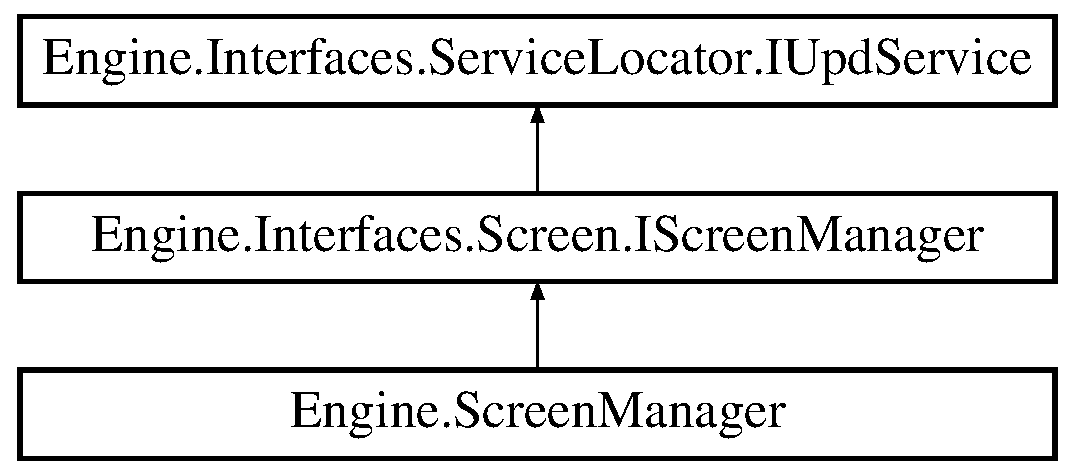
\includegraphics[height=3.000000cm]{d0/d29/a00470}
\end{center}
\end{figure}
\subsection*{Public Member Functions}
\begin{DoxyCompactItemize}
\item 
void \hyperlink{a00470_ae37c13c038cdb202262013731985eb10}{Initialize} ()
\begin{DoxyCompactList}\small\item\em M\+E\+T\+H\+OD\+: Initialise the Manager and add the first screen to be loaded \end{DoxyCompactList}\item 
void \hyperlink{a00470_a8d30874c7b1b2728a784de0c6e6f80e3}{Unlo\+Enginecreens} ()
\begin{DoxyCompactList}\small\item\em M\+E\+T\+H\+OD\+: Unload any screens that need to be unloaded \end{DoxyCompactList}\item 
void \hyperlink{a00470_afc42708b653397ca8a3a81dc8d244c61}{Update} (Game\+Time game\+Time)
\begin{DoxyCompactList}\small\item\em M\+E\+T\+H\+OD\+: Update the manager \end{DoxyCompactList}\item 
void \hyperlink{a00470_a28a87245d63c8df1634598b3d20a14cf}{Draw} (Sprite\+Batch sprite\+Batch)
\begin{DoxyCompactList}\small\item\em M\+E\+T\+H\+OD\+: Draw any objects that require drawing \end{DoxyCompactList}\item 
void \hyperlink{a00470_aba0b8f29600dabc2a55dde4d5e00c7bc}{Add} (string screen\+Name)
\begin{DoxyCompactList}\small\item\em M\+E\+T\+H\+OD\+: Add a new screen to the stack of screens to be loaded and displayed \end{DoxyCompactList}\item 
void \hyperlink{a00470_aaa6bfa9a986729ada7dcea6ac40f078d}{Replace\+Screen} (string screen\+Name)
\begin{DoxyCompactList}\small\item\em M\+E\+T\+H\+OD\+: Replace the current screen \end{DoxyCompactList}\item 
void \hyperlink{a00470_a40fbf0a98c186ba93837f6279ad2f7dd}{Check\+Screens} ()
\begin{DoxyCompactList}\small\item\em M\+E\+T\+H\+OD\+: Check if any of the screens in the stack are the same as the current screen and makes them active if so \end{DoxyCompactList}\item 
void \hyperlink{a00470_a833b8050119cd9a87efbfa23197457c9}{Check\+Screen\+Manager\+Input} ()
\begin{DoxyCompactList}\small\item\em M\+E\+T\+H\+OD\+: check for input to select different options and move between different screens \end{DoxyCompactList}\item 
void \hyperlink{a00470_a91b5204271edf5e137a85d3f8f3876d8}{Remove\+Top\+Screen} ()
\begin{DoxyCompactList}\small\item\em M\+E\+T\+H\+OD\+: Unloads and removes the top screen from the stack, essentially going back one screen \end{DoxyCompactList}\item 
void \hyperlink{a00470_aff4347b40d3fd6173e0c420adbf1146f}{Update\+Top\+Screen} (Game\+Time game\+Time)
\begin{DoxyCompactList}\small\item\em M\+E\+T\+H\+OD\+: Call the update method of the top screen \end{DoxyCompactList}\end{DoxyCompactItemize}
\subsection*{Properties}
\begin{DoxyCompactItemize}
\item 
Content\+Manager \hyperlink{a00470_a6409574161f945f4b0bd089fcc7e1014}{content}\hspace{0.3cm}{\ttfamily  \mbox{[}get, set\mbox{]}}
\begin{DoxyCompactList}\small\item\em G\+ET\+: S\+ET\+: Monogame Content\+Manager \end{DoxyCompactList}\end{DoxyCompactItemize}


\subsection{Detailed Description}
I\+N\+T\+E\+R\+F\+A\+CE\+: This interface holds the implementation for the \hyperlink{a00538}{Screen\+Manager} which is responsible for loading the content in each screen and displaying each screen. The \hyperlink{a00538}{Screen\+Manager} contains a stack of screens which allows for multiple screens to be prepared for loading whilst only one is an active screen 



\subsection{Member Function Documentation}
\mbox{\Hypertarget{a00470_aba0b8f29600dabc2a55dde4d5e00c7bc}\label{a00470_aba0b8f29600dabc2a55dde4d5e00c7bc}} 
\index{Engine\+::\+Interfaces\+::\+Screen\+::\+I\+Screen\+Manager@{Engine\+::\+Interfaces\+::\+Screen\+::\+I\+Screen\+Manager}!Add@{Add}}
\index{Add@{Add}!Engine\+::\+Interfaces\+::\+Screen\+::\+I\+Screen\+Manager@{Engine\+::\+Interfaces\+::\+Screen\+::\+I\+Screen\+Manager}}
\subsubsection{\texorpdfstring{Add()}{Add()}}
{\footnotesize\ttfamily void Engine.\+Interfaces.\+Screen.\+I\+Screen\+Manager.\+Add (\begin{DoxyParamCaption}\item[{string}]{screen\+Name }\end{DoxyParamCaption})}



M\+E\+T\+H\+OD\+: Add a new screen to the stack of screens to be loaded and displayed 


\begin{DoxyParams}{Parameters}
{\em screen\+Name} & The name of the screen to be added\\
\hline
\end{DoxyParams}


Implemented in \hyperlink{a00538_ae459e146f1e05789c4d5828cca4dead7}{Engine.\+Screen\+Manager}.

\mbox{\Hypertarget{a00470_a833b8050119cd9a87efbfa23197457c9}\label{a00470_a833b8050119cd9a87efbfa23197457c9}} 
\index{Engine\+::\+Interfaces\+::\+Screen\+::\+I\+Screen\+Manager@{Engine\+::\+Interfaces\+::\+Screen\+::\+I\+Screen\+Manager}!Check\+Screen\+Manager\+Input@{Check\+Screen\+Manager\+Input}}
\index{Check\+Screen\+Manager\+Input@{Check\+Screen\+Manager\+Input}!Engine\+::\+Interfaces\+::\+Screen\+::\+I\+Screen\+Manager@{Engine\+::\+Interfaces\+::\+Screen\+::\+I\+Screen\+Manager}}
\subsubsection{\texorpdfstring{Check\+Screen\+Manager\+Input()}{CheckScreenManagerInput()}}
{\footnotesize\ttfamily void Engine.\+Interfaces.\+Screen.\+I\+Screen\+Manager.\+Check\+Screen\+Manager\+Input (\begin{DoxyParamCaption}{ }\end{DoxyParamCaption})}



M\+E\+T\+H\+OD\+: check for input to select different options and move between different screens 



Implemented in \hyperlink{a00538_aa8e3ecdc7ae78094b07af944c31f90a9}{Engine.\+Screen\+Manager}.

\mbox{\Hypertarget{a00470_a40fbf0a98c186ba93837f6279ad2f7dd}\label{a00470_a40fbf0a98c186ba93837f6279ad2f7dd}} 
\index{Engine\+::\+Interfaces\+::\+Screen\+::\+I\+Screen\+Manager@{Engine\+::\+Interfaces\+::\+Screen\+::\+I\+Screen\+Manager}!Check\+Screens@{Check\+Screens}}
\index{Check\+Screens@{Check\+Screens}!Engine\+::\+Interfaces\+::\+Screen\+::\+I\+Screen\+Manager@{Engine\+::\+Interfaces\+::\+Screen\+::\+I\+Screen\+Manager}}
\subsubsection{\texorpdfstring{Check\+Screens()}{CheckScreens()}}
{\footnotesize\ttfamily void Engine.\+Interfaces.\+Screen.\+I\+Screen\+Manager.\+Check\+Screens (\begin{DoxyParamCaption}{ }\end{DoxyParamCaption})}



M\+E\+T\+H\+OD\+: Check if any of the screens in the stack are the same as the current screen and makes them active if so 



Implemented in \hyperlink{a00538_abe1bf121b368a6d205706da54d949ace}{Engine.\+Screen\+Manager}.

\mbox{\Hypertarget{a00470_a28a87245d63c8df1634598b3d20a14cf}\label{a00470_a28a87245d63c8df1634598b3d20a14cf}} 
\index{Engine\+::\+Interfaces\+::\+Screen\+::\+I\+Screen\+Manager@{Engine\+::\+Interfaces\+::\+Screen\+::\+I\+Screen\+Manager}!Draw@{Draw}}
\index{Draw@{Draw}!Engine\+::\+Interfaces\+::\+Screen\+::\+I\+Screen\+Manager@{Engine\+::\+Interfaces\+::\+Screen\+::\+I\+Screen\+Manager}}
\subsubsection{\texorpdfstring{Draw()}{Draw()}}
{\footnotesize\ttfamily void Engine.\+Interfaces.\+Screen.\+I\+Screen\+Manager.\+Draw (\begin{DoxyParamCaption}\item[{Sprite\+Batch}]{sprite\+Batch }\end{DoxyParamCaption})}



M\+E\+T\+H\+OD\+: Draw any objects that require drawing 


\begin{DoxyParams}{Parameters}
{\em sprite\+Batch} & Monogame Sprite\+Batch property\\
\hline
\end{DoxyParams}


Implemented in \hyperlink{a00538_a1177fbd3eb0a300167e4fa99930025e1}{Engine.\+Screen\+Manager}.

\mbox{\Hypertarget{a00470_ae37c13c038cdb202262013731985eb10}\label{a00470_ae37c13c038cdb202262013731985eb10}} 
\index{Engine\+::\+Interfaces\+::\+Screen\+::\+I\+Screen\+Manager@{Engine\+::\+Interfaces\+::\+Screen\+::\+I\+Screen\+Manager}!Initialize@{Initialize}}
\index{Initialize@{Initialize}!Engine\+::\+Interfaces\+::\+Screen\+::\+I\+Screen\+Manager@{Engine\+::\+Interfaces\+::\+Screen\+::\+I\+Screen\+Manager}}
\subsubsection{\texorpdfstring{Initialize()}{Initialize()}}
{\footnotesize\ttfamily void Engine.\+Interfaces.\+Screen.\+I\+Screen\+Manager.\+Initialize (\begin{DoxyParamCaption}{ }\end{DoxyParamCaption})}



M\+E\+T\+H\+OD\+: Initialise the Manager and add the first screen to be loaded 



Implemented in \hyperlink{a00538_aaa2b6fe0b50cf126bbb0a9b39fac1b83}{Engine.\+Screen\+Manager}.

\mbox{\Hypertarget{a00470_a91b5204271edf5e137a85d3f8f3876d8}\label{a00470_a91b5204271edf5e137a85d3f8f3876d8}} 
\index{Engine\+::\+Interfaces\+::\+Screen\+::\+I\+Screen\+Manager@{Engine\+::\+Interfaces\+::\+Screen\+::\+I\+Screen\+Manager}!Remove\+Top\+Screen@{Remove\+Top\+Screen}}
\index{Remove\+Top\+Screen@{Remove\+Top\+Screen}!Engine\+::\+Interfaces\+::\+Screen\+::\+I\+Screen\+Manager@{Engine\+::\+Interfaces\+::\+Screen\+::\+I\+Screen\+Manager}}
\subsubsection{\texorpdfstring{Remove\+Top\+Screen()}{RemoveTopScreen()}}
{\footnotesize\ttfamily void Engine.\+Interfaces.\+Screen.\+I\+Screen\+Manager.\+Remove\+Top\+Screen (\begin{DoxyParamCaption}{ }\end{DoxyParamCaption})}



M\+E\+T\+H\+OD\+: Unloads and removes the top screen from the stack, essentially going back one screen 



Implemented in \hyperlink{a00538_ab553bead481adc65547a323af9dab2d5}{Engine.\+Screen\+Manager}.

\mbox{\Hypertarget{a00470_aaa6bfa9a986729ada7dcea6ac40f078d}\label{a00470_aaa6bfa9a986729ada7dcea6ac40f078d}} 
\index{Engine\+::\+Interfaces\+::\+Screen\+::\+I\+Screen\+Manager@{Engine\+::\+Interfaces\+::\+Screen\+::\+I\+Screen\+Manager}!Replace\+Screen@{Replace\+Screen}}
\index{Replace\+Screen@{Replace\+Screen}!Engine\+::\+Interfaces\+::\+Screen\+::\+I\+Screen\+Manager@{Engine\+::\+Interfaces\+::\+Screen\+::\+I\+Screen\+Manager}}
\subsubsection{\texorpdfstring{Replace\+Screen()}{ReplaceScreen()}}
{\footnotesize\ttfamily void Engine.\+Interfaces.\+Screen.\+I\+Screen\+Manager.\+Replace\+Screen (\begin{DoxyParamCaption}\item[{string}]{screen\+Name }\end{DoxyParamCaption})}



M\+E\+T\+H\+OD\+: Replace the current screen 


\begin{DoxyParams}{Parameters}
{\em screen\+Name} & The name of the screen which will replace the screen\\
\hline
\end{DoxyParams}


Implemented in \hyperlink{a00538_a28af5b838f4345834dc2351e06c3d654}{Engine.\+Screen\+Manager}.

\mbox{\Hypertarget{a00470_a8d30874c7b1b2728a784de0c6e6f80e3}\label{a00470_a8d30874c7b1b2728a784de0c6e6f80e3}} 
\index{Engine\+::\+Interfaces\+::\+Screen\+::\+I\+Screen\+Manager@{Engine\+::\+Interfaces\+::\+Screen\+::\+I\+Screen\+Manager}!Unlo\+Enginecreens@{Unlo\+Enginecreens}}
\index{Unlo\+Enginecreens@{Unlo\+Enginecreens}!Engine\+::\+Interfaces\+::\+Screen\+::\+I\+Screen\+Manager@{Engine\+::\+Interfaces\+::\+Screen\+::\+I\+Screen\+Manager}}
\subsubsection{\texorpdfstring{Unlo\+Enginecreens()}{UnloEnginecreens()}}
{\footnotesize\ttfamily void Engine.\+Interfaces.\+Screen.\+I\+Screen\+Manager.\+Unlo\+Enginecreens (\begin{DoxyParamCaption}{ }\end{DoxyParamCaption})}



M\+E\+T\+H\+OD\+: Unload any screens that need to be unloaded 



Implemented in \hyperlink{a00538_a1e85d6cc74fdb929f4729d1170886fb4}{Engine.\+Screen\+Manager}.

\mbox{\Hypertarget{a00470_afc42708b653397ca8a3a81dc8d244c61}\label{a00470_afc42708b653397ca8a3a81dc8d244c61}} 
\index{Engine\+::\+Interfaces\+::\+Screen\+::\+I\+Screen\+Manager@{Engine\+::\+Interfaces\+::\+Screen\+::\+I\+Screen\+Manager}!Update@{Update}}
\index{Update@{Update}!Engine\+::\+Interfaces\+::\+Screen\+::\+I\+Screen\+Manager@{Engine\+::\+Interfaces\+::\+Screen\+::\+I\+Screen\+Manager}}
\subsubsection{\texorpdfstring{Update()}{Update()}}
{\footnotesize\ttfamily void Engine.\+Interfaces.\+Screen.\+I\+Screen\+Manager.\+Update (\begin{DoxyParamCaption}\item[{Game\+Time}]{game\+Time }\end{DoxyParamCaption})}



M\+E\+T\+H\+OD\+: Update the manager 


\begin{DoxyParams}{Parameters}
{\em game\+Time} & Monogame Game\+Time property\\
\hline
\end{DoxyParams}


Implements \hyperlink{a00478_a387fce2a5440a4dc63f8d72772ecbdaa}{Engine.\+Interfaces.\+Service\+Locator.\+I\+Upd\+Service}.



Implemented in \hyperlink{a00538_a9abaa968b161ebb2b84c7a47ada52f90}{Engine.\+Screen\+Manager}.

\mbox{\Hypertarget{a00470_aff4347b40d3fd6173e0c420adbf1146f}\label{a00470_aff4347b40d3fd6173e0c420adbf1146f}} 
\index{Engine\+::\+Interfaces\+::\+Screen\+::\+I\+Screen\+Manager@{Engine\+::\+Interfaces\+::\+Screen\+::\+I\+Screen\+Manager}!Update\+Top\+Screen@{Update\+Top\+Screen}}
\index{Update\+Top\+Screen@{Update\+Top\+Screen}!Engine\+::\+Interfaces\+::\+Screen\+::\+I\+Screen\+Manager@{Engine\+::\+Interfaces\+::\+Screen\+::\+I\+Screen\+Manager}}
\subsubsection{\texorpdfstring{Update\+Top\+Screen()}{UpdateTopScreen()}}
{\footnotesize\ttfamily void Engine.\+Interfaces.\+Screen.\+I\+Screen\+Manager.\+Update\+Top\+Screen (\begin{DoxyParamCaption}\item[{Game\+Time}]{game\+Time }\end{DoxyParamCaption})}



M\+E\+T\+H\+OD\+: Call the update method of the top screen 


\begin{DoxyParams}{Parameters}
{\em game\+Time} & \\
\hline
\end{DoxyParams}


Implemented in \hyperlink{a00538_a59b04e135a3b2a75a608752e2bfabc77}{Engine.\+Screen\+Manager}.



\subsection{Property Documentation}
\mbox{\Hypertarget{a00470_a6409574161f945f4b0bd089fcc7e1014}\label{a00470_a6409574161f945f4b0bd089fcc7e1014}} 
\index{Engine\+::\+Interfaces\+::\+Screen\+::\+I\+Screen\+Manager@{Engine\+::\+Interfaces\+::\+Screen\+::\+I\+Screen\+Manager}!content@{content}}
\index{content@{content}!Engine\+::\+Interfaces\+::\+Screen\+::\+I\+Screen\+Manager@{Engine\+::\+Interfaces\+::\+Screen\+::\+I\+Screen\+Manager}}
\subsubsection{\texorpdfstring{content}{content}}
{\footnotesize\ttfamily Content\+Manager Engine.\+Interfaces.\+Screen.\+I\+Screen\+Manager.\+content\hspace{0.3cm}{\ttfamily [get]}, {\ttfamily [set]}}



G\+ET\+: S\+ET\+: Monogame Content\+Manager 



The documentation for this interface was generated from the following file\+:\begin{DoxyCompactItemize}
\item 
\hyperlink{a00134}{I\+Screen\+Manager.\+cs}\end{DoxyCompactItemize}

\hypertarget{a00474}{}\section{Engine.\+Interfaces.\+Service\+Locator.\+I\+Service\+Locator Interface Reference}
\label{a00474}\index{Engine.\+Interfaces.\+Service\+Locator.\+I\+Service\+Locator@{Engine.\+Interfaces.\+Service\+Locator.\+I\+Service\+Locator}}


I\+N\+T\+E\+R\+F\+A\+CE\+: An Interface holding the implementation for the Service Locator which removes the need for singletons throughout the engine  


Inheritance diagram for Engine.\+Interfaces.\+Service\+Locator.\+I\+Service\+Locator\+:\begin{figure}[H]
\begin{center}
\leavevmode
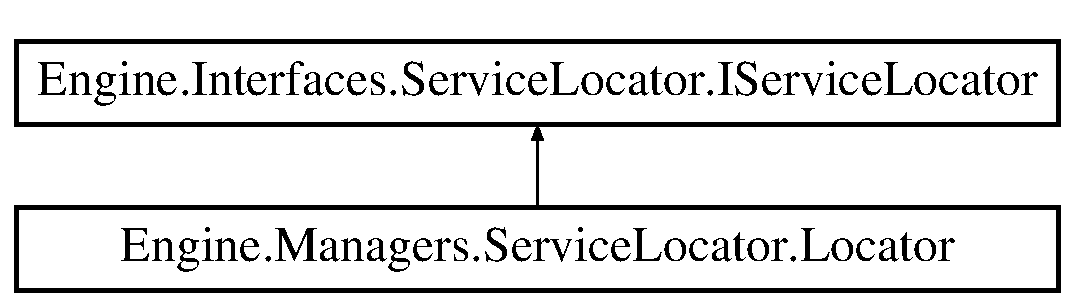
\includegraphics[height=2.000000cm]{d5/d26/a00474}
\end{center}
\end{figure}
\subsection*{Public Member Functions}
\begin{DoxyCompactItemize}
\item 
T \hyperlink{a00474_a39ce84b8fb97655fd7039be3c4fa5f1c}{get\+Service$<$ T $>$} ()
\begin{DoxyCompactList}\small\item\em M\+E\+T\+H\+OD\+: Return a service, T is a generic type of Manager \end{DoxyCompactList}\item 
void \hyperlink{a00474_a4bf9f6979adf99eda26320a420262991}{Initialize\+Services} (Content\+Manager c, Sprite\+Batch sb)
\begin{DoxyCompactList}\small\item\em M\+E\+T\+H\+OD\+: Initialises the services upon the running of the program so that they all exist and can be accessed \end{DoxyCompactList}\item 
void \hyperlink{a00474_a5bf3aab2adcf14c813a348325003ddcc}{Update\+Services} (Game\+Time game\+Time)
\begin{DoxyCompactList}\small\item\em Loops through and updates each service in turn. \end{DoxyCompactList}\end{DoxyCompactItemize}


\subsection{Detailed Description}
I\+N\+T\+E\+R\+F\+A\+CE\+: An Interface holding the implementation for the Service Locator which removes the need for singletons throughout the engine 



\subsection{Member Function Documentation}
\mbox{\Hypertarget{a00474_a39ce84b8fb97655fd7039be3c4fa5f1c}\label{a00474_a39ce84b8fb97655fd7039be3c4fa5f1c}} 
\index{Engine\+::\+Interfaces\+::\+Service\+Locator\+::\+I\+Service\+Locator@{Engine\+::\+Interfaces\+::\+Service\+Locator\+::\+I\+Service\+Locator}!get\+Service$<$ T $>$@{get\+Service$<$ T $>$}}
\index{get\+Service$<$ T $>$@{get\+Service$<$ T $>$}!Engine\+::\+Interfaces\+::\+Service\+Locator\+::\+I\+Service\+Locator@{Engine\+::\+Interfaces\+::\+Service\+Locator\+::\+I\+Service\+Locator}}
\subsubsection{\texorpdfstring{get\+Service$<$ T $>$()}{getService< T >()}}
{\footnotesize\ttfamily T Engine.\+Interfaces.\+Service\+Locator.\+I\+Service\+Locator.\+get\+Service$<$ T $>$ (\begin{DoxyParamCaption}{ }\end{DoxyParamCaption})}



M\+E\+T\+H\+OD\+: Return a service, T is a generic type of Manager 


\begin{DoxyTemplParams}{Template Parameters}
{\em T} & Generic Manager\\
\hline
\end{DoxyTemplParams}
\begin{DoxyReturn}{Returns}
Manager of type T
\end{DoxyReturn}


Implemented in \hyperlink{a00542_a2bb3c0174bd67904d148bc789c9faaba}{Engine.\+Managers.\+Service\+Locator.\+Locator}.

\mbox{\Hypertarget{a00474_a4bf9f6979adf99eda26320a420262991}\label{a00474_a4bf9f6979adf99eda26320a420262991}} 
\index{Engine\+::\+Interfaces\+::\+Service\+Locator\+::\+I\+Service\+Locator@{Engine\+::\+Interfaces\+::\+Service\+Locator\+::\+I\+Service\+Locator}!Initialize\+Services@{Initialize\+Services}}
\index{Initialize\+Services@{Initialize\+Services}!Engine\+::\+Interfaces\+::\+Service\+Locator\+::\+I\+Service\+Locator@{Engine\+::\+Interfaces\+::\+Service\+Locator\+::\+I\+Service\+Locator}}
\subsubsection{\texorpdfstring{Initialize\+Services()}{InitializeServices()}}
{\footnotesize\ttfamily void Engine.\+Interfaces.\+Service\+Locator.\+I\+Service\+Locator.\+Initialize\+Services (\begin{DoxyParamCaption}\item[{Content\+Manager}]{c,  }\item[{Sprite\+Batch}]{sb }\end{DoxyParamCaption})}



M\+E\+T\+H\+OD\+: Initialises the services upon the running of the program so that they all exist and can be accessed 


\begin{DoxyParams}{Parameters}
{\em c} & Monogame Content\+Manager\\
\hline
{\em sb} & Monogame Spritebatch for any drawing\\
\hline
\end{DoxyParams}


Implemented in \hyperlink{a00542_a34bc6f5d735512bae556d2ec65a7bda7}{Engine.\+Managers.\+Service\+Locator.\+Locator}.

\mbox{\Hypertarget{a00474_a5bf3aab2adcf14c813a348325003ddcc}\label{a00474_a5bf3aab2adcf14c813a348325003ddcc}} 
\index{Engine\+::\+Interfaces\+::\+Service\+Locator\+::\+I\+Service\+Locator@{Engine\+::\+Interfaces\+::\+Service\+Locator\+::\+I\+Service\+Locator}!Update\+Services@{Update\+Services}}
\index{Update\+Services@{Update\+Services}!Engine\+::\+Interfaces\+::\+Service\+Locator\+::\+I\+Service\+Locator@{Engine\+::\+Interfaces\+::\+Service\+Locator\+::\+I\+Service\+Locator}}
\subsubsection{\texorpdfstring{Update\+Services()}{UpdateServices()}}
{\footnotesize\ttfamily void Engine.\+Interfaces.\+Service\+Locator.\+I\+Service\+Locator.\+Update\+Services (\begin{DoxyParamCaption}\item[{Game\+Time}]{game\+Time }\end{DoxyParamCaption})}



Loops through and updates each service in turn. 


\begin{DoxyParams}{Parameters}
{\em game\+Time} & \\
\hline
\end{DoxyParams}


Implemented in \hyperlink{a00542_ab66a423db26d79e6fc655df699a64f0c}{Engine.\+Managers.\+Service\+Locator.\+Locator}.



The documentation for this interface was generated from the following file\+:\begin{DoxyCompactItemize}
\item 
\hyperlink{a00137}{I\+Service\+Locator.\+cs}\end{DoxyCompactItemize}

\hypertarget{a00482}{}\section{Engine.\+Interfaces.\+Sound.\+I\+Sound\+Manager Interface Reference}
\label{a00482}\index{Engine.\+Interfaces.\+Sound.\+I\+Sound\+Manager@{Engine.\+Interfaces.\+Sound.\+I\+Sound\+Manager}}


I\+N\+T\+E\+R\+F\+A\+CE\+: Holds the implementation for the sound manager which is responsible for the storage and playback of sound files.  


Inheritance diagram for Engine.\+Interfaces.\+Sound.\+I\+Sound\+Manager\+:\begin{figure}[H]
\begin{center}
\leavevmode
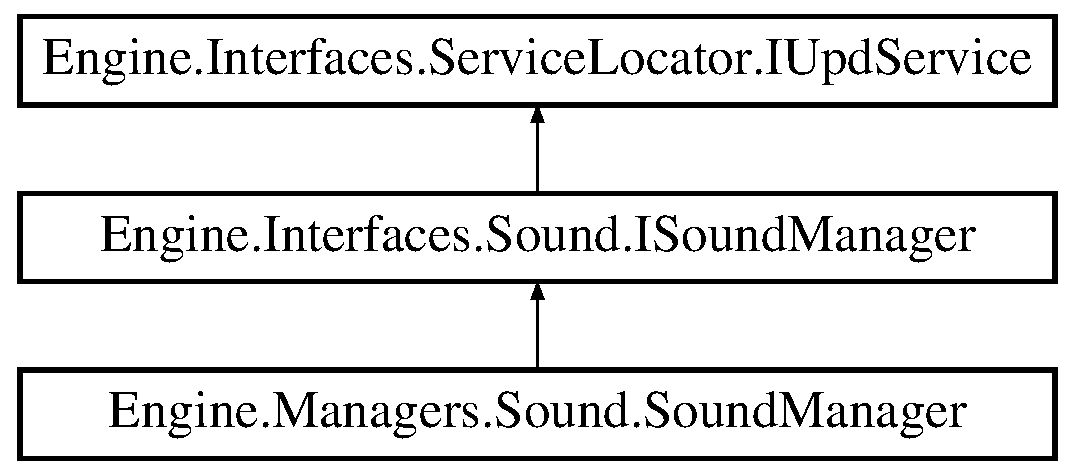
\includegraphics[height=3.000000cm]{db/d8e/a00482}
\end{center}
\end{figure}
\subsection*{Public Member Functions}
\begin{DoxyCompactItemize}
\item 
void \hyperlink{a00482_a02f14f3401f425a686a50e6b6a40aca7}{Initialize} ()
\begin{DoxyCompactList}\small\item\em M\+E\+T\+H\+OD\+: Initialises the logic of the Manager \end{DoxyCompactList}\item 
void \hyperlink{a00482_aec02346c5397b9b01b9d5d6baedc923e}{Play} (string name)
\begin{DoxyCompactList}\small\item\em M\+E\+T\+H\+OD\+: Plays the song of the name provided \end{DoxyCompactList}\item 
void \hyperlink{a00482_aa9e2fb77a5fe624ce65373f5ee8328ae}{Play\+Effect} (string name)
\begin{DoxyCompactList}\small\item\em M\+E\+T\+H\+OD\+: Plays the sound effect of the name provided \end{DoxyCompactList}\item 
void \hyperlink{a00482_a5bcad4d517b37a12b17e59d0b927ca37}{Mute} ()
\begin{DoxyCompactList}\small\item\em M\+E\+T\+H\+OD\+: Mutes all sound \end{DoxyCompactList}\item 
void \hyperlink{a00482_a59c011a4cf667d6e967bddad50c7cb2f}{un\+Mute} ()
\begin{DoxyCompactList}\small\item\em M\+E\+T\+H\+OD\+: Unmutes all sound \end{DoxyCompactList}\item 
void \hyperlink{a00482_ada3f38d5c50655b55f146ccdaf7c5967}{Volume} (float Volume)
\begin{DoxyCompactList}\small\item\em M\+E\+T\+H\+OD\+: changes the volume of sound played \end{DoxyCompactList}\item 
void \hyperlink{a00482_ac47a91d3e28a8f7a1e5348fb6eff50e2}{Stop} ()
\begin{DoxyCompactList}\small\item\em M\+E\+T\+H\+OD\+: Stops the current sound being played \end{DoxyCompactList}\item 
void \hyperlink{a00482_af7ddcb52a6283aa2cf4392c75d2a0cff}{Update} (Game\+Time game\+Time)
\begin{DoxyCompactList}\small\item\em M\+E\+T\+H\+OD\+: the update loop cycled through each frame \end{DoxyCompactList}\item 
void \hyperlink{a00482_afe3eaaed21c8b64692bc338309ac4a4d}{vol\+Up} ()
\begin{DoxyCompactList}\small\item\em M\+E\+T\+H\+OD\+: Increases the volume slightly \end{DoxyCompactList}\item 
void \hyperlink{a00482_a96629b32d608ca84fe1a3624bece7f05}{vol\+Down} ()
\begin{DoxyCompactList}\small\item\em M\+E\+T\+H\+OD\+: Decreases the volume slightly \end{DoxyCompactList}\item 
void \hyperlink{a00482_a8aa47dcffde058c1146f7ebf5b0edb84}{on\+Screen\+Changed} (\hyperlink{a00550}{Base\+Screen} screen)
\begin{DoxyCompactList}\small\item\em M\+E\+T\+H\+OD\+: Plays the sound of the screen that is being changed to \end{DoxyCompactList}\end{DoxyCompactItemize}
\subsection*{Properties}
\begin{DoxyCompactItemize}
\item 
bool \hyperlink{a00482_ac8a262a7db42a3802a58c9a7e0a471ca}{is\+Muted}\hspace{0.3cm}{\ttfamily  \mbox{[}get, set\mbox{]}}
\end{DoxyCompactItemize}


\subsection{Detailed Description}
I\+N\+T\+E\+R\+F\+A\+CE\+: Holds the implementation for the sound manager which is responsible for the storage and playback of sound files. 



\subsection{Member Function Documentation}
\mbox{\Hypertarget{a00482_a02f14f3401f425a686a50e6b6a40aca7}\label{a00482_a02f14f3401f425a686a50e6b6a40aca7}} 
\index{Engine\+::\+Interfaces\+::\+Sound\+::\+I\+Sound\+Manager@{Engine\+::\+Interfaces\+::\+Sound\+::\+I\+Sound\+Manager}!Initialize@{Initialize}}
\index{Initialize@{Initialize}!Engine\+::\+Interfaces\+::\+Sound\+::\+I\+Sound\+Manager@{Engine\+::\+Interfaces\+::\+Sound\+::\+I\+Sound\+Manager}}
\subsubsection{\texorpdfstring{Initialize()}{Initialize()}}
{\footnotesize\ttfamily void Engine.\+Interfaces.\+Sound.\+I\+Sound\+Manager.\+Initialize (\begin{DoxyParamCaption}{ }\end{DoxyParamCaption})}



M\+E\+T\+H\+OD\+: Initialises the logic of the Manager 



Implemented in \hyperlink{a00546_a06224065983b6fe162de98b8dcc944c2}{Engine.\+Managers.\+Sound.\+Sound\+Manager}.

\mbox{\Hypertarget{a00482_a5bcad4d517b37a12b17e59d0b927ca37}\label{a00482_a5bcad4d517b37a12b17e59d0b927ca37}} 
\index{Engine\+::\+Interfaces\+::\+Sound\+::\+I\+Sound\+Manager@{Engine\+::\+Interfaces\+::\+Sound\+::\+I\+Sound\+Manager}!Mute@{Mute}}
\index{Mute@{Mute}!Engine\+::\+Interfaces\+::\+Sound\+::\+I\+Sound\+Manager@{Engine\+::\+Interfaces\+::\+Sound\+::\+I\+Sound\+Manager}}
\subsubsection{\texorpdfstring{Mute()}{Mute()}}
{\footnotesize\ttfamily void Engine.\+Interfaces.\+Sound.\+I\+Sound\+Manager.\+Mute (\begin{DoxyParamCaption}{ }\end{DoxyParamCaption})}



M\+E\+T\+H\+OD\+: Mutes all sound 



Implemented in \hyperlink{a00546_a5a3a9b96e6708deedf2c4939b3259011}{Engine.\+Managers.\+Sound.\+Sound\+Manager}.

\mbox{\Hypertarget{a00482_a8aa47dcffde058c1146f7ebf5b0edb84}\label{a00482_a8aa47dcffde058c1146f7ebf5b0edb84}} 
\index{Engine\+::\+Interfaces\+::\+Sound\+::\+I\+Sound\+Manager@{Engine\+::\+Interfaces\+::\+Sound\+::\+I\+Sound\+Manager}!on\+Screen\+Changed@{on\+Screen\+Changed}}
\index{on\+Screen\+Changed@{on\+Screen\+Changed}!Engine\+::\+Interfaces\+::\+Sound\+::\+I\+Sound\+Manager@{Engine\+::\+Interfaces\+::\+Sound\+::\+I\+Sound\+Manager}}
\subsubsection{\texorpdfstring{on\+Screen\+Changed()}{onScreenChanged()}}
{\footnotesize\ttfamily void Engine.\+Interfaces.\+Sound.\+I\+Sound\+Manager.\+on\+Screen\+Changed (\begin{DoxyParamCaption}\item[{\hyperlink{a00550}{Base\+Screen}}]{screen }\end{DoxyParamCaption})}



M\+E\+T\+H\+OD\+: Plays the sound of the screen that is being changed to 


\begin{DoxyParams}{Parameters}
{\em screen} & The screen being changed to\\
\hline
\end{DoxyParams}


Implemented in \hyperlink{a00546_a8dfbb15525871b87e6cdcf744b070139}{Engine.\+Managers.\+Sound.\+Sound\+Manager}.

\mbox{\Hypertarget{a00482_aec02346c5397b9b01b9d5d6baedc923e}\label{a00482_aec02346c5397b9b01b9d5d6baedc923e}} 
\index{Engine\+::\+Interfaces\+::\+Sound\+::\+I\+Sound\+Manager@{Engine\+::\+Interfaces\+::\+Sound\+::\+I\+Sound\+Manager}!Play@{Play}}
\index{Play@{Play}!Engine\+::\+Interfaces\+::\+Sound\+::\+I\+Sound\+Manager@{Engine\+::\+Interfaces\+::\+Sound\+::\+I\+Sound\+Manager}}
\subsubsection{\texorpdfstring{Play()}{Play()}}
{\footnotesize\ttfamily void Engine.\+Interfaces.\+Sound.\+I\+Sound\+Manager.\+Play (\begin{DoxyParamCaption}\item[{string}]{name }\end{DoxyParamCaption})}



M\+E\+T\+H\+OD\+: Plays the song of the name provided 


\begin{DoxyParams}{Parameters}
{\em name} & The name of the song to be played\\
\hline
\end{DoxyParams}


Implemented in \hyperlink{a00546_aabfeb911d8bd573065e9c02d3f81e582}{Engine.\+Managers.\+Sound.\+Sound\+Manager}.

\mbox{\Hypertarget{a00482_aa9e2fb77a5fe624ce65373f5ee8328ae}\label{a00482_aa9e2fb77a5fe624ce65373f5ee8328ae}} 
\index{Engine\+::\+Interfaces\+::\+Sound\+::\+I\+Sound\+Manager@{Engine\+::\+Interfaces\+::\+Sound\+::\+I\+Sound\+Manager}!Play\+Effect@{Play\+Effect}}
\index{Play\+Effect@{Play\+Effect}!Engine\+::\+Interfaces\+::\+Sound\+::\+I\+Sound\+Manager@{Engine\+::\+Interfaces\+::\+Sound\+::\+I\+Sound\+Manager}}
\subsubsection{\texorpdfstring{Play\+Effect()}{PlayEffect()}}
{\footnotesize\ttfamily void Engine.\+Interfaces.\+Sound.\+I\+Sound\+Manager.\+Play\+Effect (\begin{DoxyParamCaption}\item[{string}]{name }\end{DoxyParamCaption})}



M\+E\+T\+H\+OD\+: Plays the sound effect of the name provided 


\begin{DoxyParams}{Parameters}
{\em name} & The name of the sound effect to be played\\
\hline
\end{DoxyParams}


Implemented in \hyperlink{a00546_a6613813ccd38703484e80ca8775ecdf8}{Engine.\+Managers.\+Sound.\+Sound\+Manager}.

\mbox{\Hypertarget{a00482_ac47a91d3e28a8f7a1e5348fb6eff50e2}\label{a00482_ac47a91d3e28a8f7a1e5348fb6eff50e2}} 
\index{Engine\+::\+Interfaces\+::\+Sound\+::\+I\+Sound\+Manager@{Engine\+::\+Interfaces\+::\+Sound\+::\+I\+Sound\+Manager}!Stop@{Stop}}
\index{Stop@{Stop}!Engine\+::\+Interfaces\+::\+Sound\+::\+I\+Sound\+Manager@{Engine\+::\+Interfaces\+::\+Sound\+::\+I\+Sound\+Manager}}
\subsubsection{\texorpdfstring{Stop()}{Stop()}}
{\footnotesize\ttfamily void Engine.\+Interfaces.\+Sound.\+I\+Sound\+Manager.\+Stop (\begin{DoxyParamCaption}{ }\end{DoxyParamCaption})}



M\+E\+T\+H\+OD\+: Stops the current sound being played 



Implemented in \hyperlink{a00546_a0d3222475855f63b0c8f9dbe9b52e7f7}{Engine.\+Managers.\+Sound.\+Sound\+Manager}.

\mbox{\Hypertarget{a00482_a59c011a4cf667d6e967bddad50c7cb2f}\label{a00482_a59c011a4cf667d6e967bddad50c7cb2f}} 
\index{Engine\+::\+Interfaces\+::\+Sound\+::\+I\+Sound\+Manager@{Engine\+::\+Interfaces\+::\+Sound\+::\+I\+Sound\+Manager}!un\+Mute@{un\+Mute}}
\index{un\+Mute@{un\+Mute}!Engine\+::\+Interfaces\+::\+Sound\+::\+I\+Sound\+Manager@{Engine\+::\+Interfaces\+::\+Sound\+::\+I\+Sound\+Manager}}
\subsubsection{\texorpdfstring{un\+Mute()}{unMute()}}
{\footnotesize\ttfamily void Engine.\+Interfaces.\+Sound.\+I\+Sound\+Manager.\+un\+Mute (\begin{DoxyParamCaption}{ }\end{DoxyParamCaption})}



M\+E\+T\+H\+OD\+: Unmutes all sound 



Implemented in \hyperlink{a00546_ad62eb34a308bfe457bc7229045a66af0}{Engine.\+Managers.\+Sound.\+Sound\+Manager}.

\mbox{\Hypertarget{a00482_af7ddcb52a6283aa2cf4392c75d2a0cff}\label{a00482_af7ddcb52a6283aa2cf4392c75d2a0cff}} 
\index{Engine\+::\+Interfaces\+::\+Sound\+::\+I\+Sound\+Manager@{Engine\+::\+Interfaces\+::\+Sound\+::\+I\+Sound\+Manager}!Update@{Update}}
\index{Update@{Update}!Engine\+::\+Interfaces\+::\+Sound\+::\+I\+Sound\+Manager@{Engine\+::\+Interfaces\+::\+Sound\+::\+I\+Sound\+Manager}}
\subsubsection{\texorpdfstring{Update()}{Update()}}
{\footnotesize\ttfamily void Engine.\+Interfaces.\+Sound.\+I\+Sound\+Manager.\+Update (\begin{DoxyParamCaption}\item[{Game\+Time}]{game\+Time }\end{DoxyParamCaption})}



M\+E\+T\+H\+OD\+: the update loop cycled through each frame 


\begin{DoxyParams}{Parameters}
{\em game\+Time} & Monogame Game\+Time property\\
\hline
\end{DoxyParams}


Implements \hyperlink{a00478_a387fce2a5440a4dc63f8d72772ecbdaa}{Engine.\+Interfaces.\+Service\+Locator.\+I\+Upd\+Service}.



Implemented in \hyperlink{a00546_a43e47a47daa91f3b1d0f38b3dcb0323e}{Engine.\+Managers.\+Sound.\+Sound\+Manager}.

\mbox{\Hypertarget{a00482_a96629b32d608ca84fe1a3624bece7f05}\label{a00482_a96629b32d608ca84fe1a3624bece7f05}} 
\index{Engine\+::\+Interfaces\+::\+Sound\+::\+I\+Sound\+Manager@{Engine\+::\+Interfaces\+::\+Sound\+::\+I\+Sound\+Manager}!vol\+Down@{vol\+Down}}
\index{vol\+Down@{vol\+Down}!Engine\+::\+Interfaces\+::\+Sound\+::\+I\+Sound\+Manager@{Engine\+::\+Interfaces\+::\+Sound\+::\+I\+Sound\+Manager}}
\subsubsection{\texorpdfstring{vol\+Down()}{volDown()}}
{\footnotesize\ttfamily void Engine.\+Interfaces.\+Sound.\+I\+Sound\+Manager.\+vol\+Down (\begin{DoxyParamCaption}{ }\end{DoxyParamCaption})}



M\+E\+T\+H\+OD\+: Decreases the volume slightly 



Implemented in \hyperlink{a00546_a888a7942f63cc582f7b73d61b69ebbac}{Engine.\+Managers.\+Sound.\+Sound\+Manager}.

\mbox{\Hypertarget{a00482_ada3f38d5c50655b55f146ccdaf7c5967}\label{a00482_ada3f38d5c50655b55f146ccdaf7c5967}} 
\index{Engine\+::\+Interfaces\+::\+Sound\+::\+I\+Sound\+Manager@{Engine\+::\+Interfaces\+::\+Sound\+::\+I\+Sound\+Manager}!Volume@{Volume}}
\index{Volume@{Volume}!Engine\+::\+Interfaces\+::\+Sound\+::\+I\+Sound\+Manager@{Engine\+::\+Interfaces\+::\+Sound\+::\+I\+Sound\+Manager}}
\subsubsection{\texorpdfstring{Volume()}{Volume()}}
{\footnotesize\ttfamily void Engine.\+Interfaces.\+Sound.\+I\+Sound\+Manager.\+Volume (\begin{DoxyParamCaption}\item[{float}]{Volume }\end{DoxyParamCaption})}



M\+E\+T\+H\+OD\+: changes the volume of sound played 


\begin{DoxyParams}{Parameters}
{\em Volume} & The volume to be changed to\\
\hline
\end{DoxyParams}


Implemented in \hyperlink{a00546_ae1be3ecb76007fdc47843305df49604b}{Engine.\+Managers.\+Sound.\+Sound\+Manager}.

\mbox{\Hypertarget{a00482_afe3eaaed21c8b64692bc338309ac4a4d}\label{a00482_afe3eaaed21c8b64692bc338309ac4a4d}} 
\index{Engine\+::\+Interfaces\+::\+Sound\+::\+I\+Sound\+Manager@{Engine\+::\+Interfaces\+::\+Sound\+::\+I\+Sound\+Manager}!vol\+Up@{vol\+Up}}
\index{vol\+Up@{vol\+Up}!Engine\+::\+Interfaces\+::\+Sound\+::\+I\+Sound\+Manager@{Engine\+::\+Interfaces\+::\+Sound\+::\+I\+Sound\+Manager}}
\subsubsection{\texorpdfstring{vol\+Up()}{volUp()}}
{\footnotesize\ttfamily void Engine.\+Interfaces.\+Sound.\+I\+Sound\+Manager.\+vol\+Up (\begin{DoxyParamCaption}{ }\end{DoxyParamCaption})}



M\+E\+T\+H\+OD\+: Increases the volume slightly 



Implemented in \hyperlink{a00546_af9d82c533dfd90077b275f2b09ee90b0}{Engine.\+Managers.\+Sound.\+Sound\+Manager}.



\subsection{Property Documentation}
\mbox{\Hypertarget{a00482_ac8a262a7db42a3802a58c9a7e0a471ca}\label{a00482_ac8a262a7db42a3802a58c9a7e0a471ca}} 
\index{Engine\+::\+Interfaces\+::\+Sound\+::\+I\+Sound\+Manager@{Engine\+::\+Interfaces\+::\+Sound\+::\+I\+Sound\+Manager}!is\+Muted@{is\+Muted}}
\index{is\+Muted@{is\+Muted}!Engine\+::\+Interfaces\+::\+Sound\+::\+I\+Sound\+Manager@{Engine\+::\+Interfaces\+::\+Sound\+::\+I\+Sound\+Manager}}
\subsubsection{\texorpdfstring{is\+Muted}{isMuted}}
{\footnotesize\ttfamily bool Engine.\+Interfaces.\+Sound.\+I\+Sound\+Manager.\+is\+Muted\hspace{0.3cm}{\ttfamily [get]}, {\ttfamily [set]}}



The documentation for this interface was generated from the following file\+:\begin{DoxyCompactItemize}
\item 
\hyperlink{a00143}{I\+Sound\+Manager.\+cs}\end{DoxyCompactItemize}

\hypertarget{a00338}{}\section{Engine.\+Entities.\+Steering.\+I\+Steering\+Behaviour Interface Reference}
\label{a00338}\index{Engine.\+Entities.\+Steering.\+I\+Steering\+Behaviour@{Engine.\+Entities.\+Steering.\+I\+Steering\+Behaviour}}
\subsection*{Public Member Functions}
\begin{DoxyCompactItemize}
\item 
Vector2 \mbox{[}$\,$\mbox{]} \hyperlink{a00338_adef1f686b189cf585e7549595d44a2e3}{Apply\+Behaviour} ()
\end{DoxyCompactItemize}


\subsection{Member Function Documentation}
\mbox{\Hypertarget{a00338_adef1f686b189cf585e7549595d44a2e3}\label{a00338_adef1f686b189cf585e7549595d44a2e3}} 
\index{Engine\+::\+Entities\+::\+Steering\+::\+I\+Steering\+Behaviour@{Engine\+::\+Entities\+::\+Steering\+::\+I\+Steering\+Behaviour}!Apply\+Behaviour@{Apply\+Behaviour}}
\index{Apply\+Behaviour@{Apply\+Behaviour}!Engine\+::\+Entities\+::\+Steering\+::\+I\+Steering\+Behaviour@{Engine\+::\+Entities\+::\+Steering\+::\+I\+Steering\+Behaviour}}
\subsubsection{\texorpdfstring{Apply\+Behaviour()}{ApplyBehaviour()}}
{\footnotesize\ttfamily Vector2 \mbox{[}$\,$\mbox{]} Engine.\+Entities.\+Steering.\+I\+Steering\+Behaviour.\+Apply\+Behaviour (\begin{DoxyParamCaption}{ }\end{DoxyParamCaption})}



The documentation for this interface was generated from the following file\+:\begin{DoxyCompactItemize}
\item 
\hyperlink{a00035}{I\+Steering\+Behaviour.\+cs}\end{DoxyCompactItemize}

\hypertarget{a00478}{}\section{Engine.\+Interfaces.\+Service\+Locator.\+I\+Upd\+Service Interface Reference}
\label{a00478}\index{Engine.\+Interfaces.\+Service\+Locator.\+I\+Upd\+Service@{Engine.\+Interfaces.\+Service\+Locator.\+I\+Upd\+Service}}


I\+N\+T\+E\+R\+F\+A\+CE\+: All \hyperlink{a00239}{Managers} that need to be updated every frame subscribe to this interface  


Inheritance diagram for Engine.\+Interfaces.\+Service\+Locator.\+I\+Upd\+Service\+:\begin{figure}[H]
\begin{center}
\leavevmode
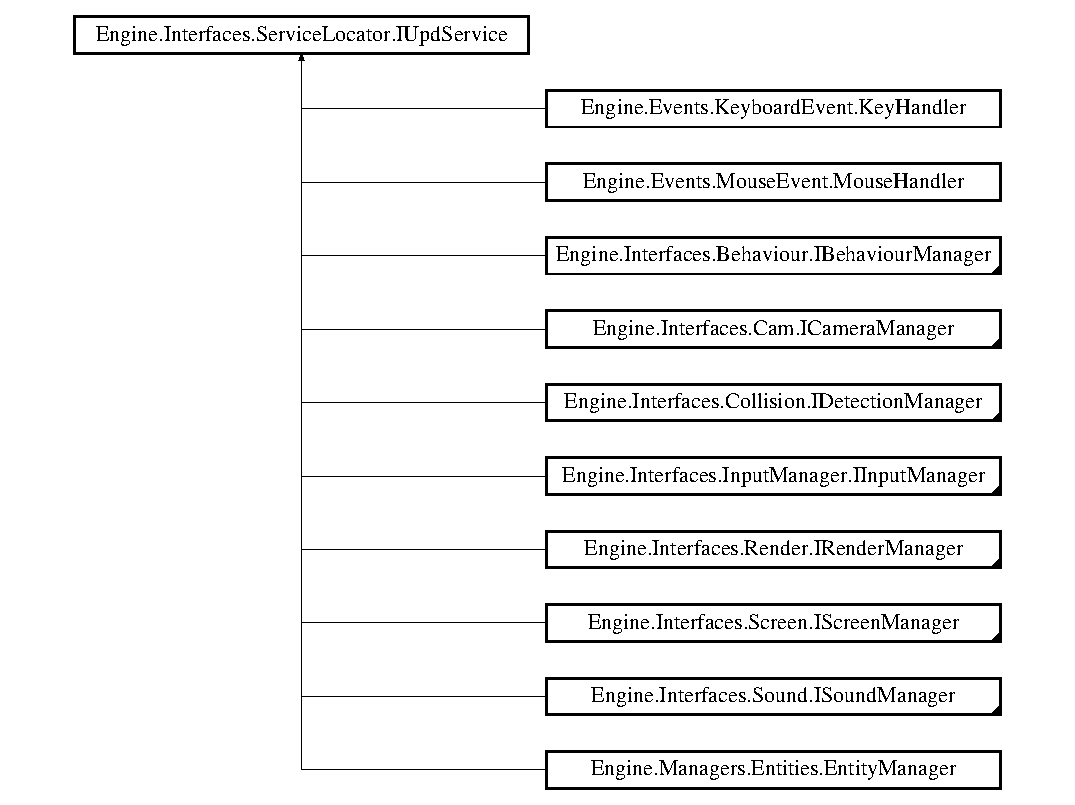
\includegraphics[height=10.370371cm]{d9/dea/a00478}
\end{center}
\end{figure}
\subsection*{Public Member Functions}
\begin{DoxyCompactItemize}
\item 
void \hyperlink{a00478_a387fce2a5440a4dc63f8d72772ecbdaa}{Update} (Game\+Time game\+Time)
\begin{DoxyCompactList}\small\item\em M\+E\+T\+H\+OD\+: The update loop which is cycled through ever frame \end{DoxyCompactList}\end{DoxyCompactItemize}


\subsection{Detailed Description}
I\+N\+T\+E\+R\+F\+A\+CE\+: All \hyperlink{a00239}{Managers} that need to be updated every frame subscribe to this interface 



\subsection{Member Function Documentation}
\mbox{\Hypertarget{a00478_a387fce2a5440a4dc63f8d72772ecbdaa}\label{a00478_a387fce2a5440a4dc63f8d72772ecbdaa}} 
\index{Engine\+::\+Interfaces\+::\+Service\+Locator\+::\+I\+Upd\+Service@{Engine\+::\+Interfaces\+::\+Service\+Locator\+::\+I\+Upd\+Service}!Update@{Update}}
\index{Update@{Update}!Engine\+::\+Interfaces\+::\+Service\+Locator\+::\+I\+Upd\+Service@{Engine\+::\+Interfaces\+::\+Service\+Locator\+::\+I\+Upd\+Service}}
\subsubsection{\texorpdfstring{Update()}{Update()}}
{\footnotesize\ttfamily void Engine.\+Interfaces.\+Service\+Locator.\+I\+Upd\+Service.\+Update (\begin{DoxyParamCaption}\item[{Game\+Time}]{game\+Time }\end{DoxyParamCaption})}



M\+E\+T\+H\+OD\+: The update loop which is cycled through ever frame 


\begin{DoxyParams}{Parameters}
{\em game\+Time} & The Mono\+Game Gametime property\\
\hline
\end{DoxyParams}


Implemented in \hyperlink{a00518_a386e96f9edb12689118de624c559de0f}{Engine.\+Managers.\+Entities.\+Entity\+Manager}, \hyperlink{a00526_a7b63b947d986ab05b66c4c9f78ee3c20}{Engine.\+Managers.\+Render.\+Render\+Manager}, \hyperlink{a00486_a729bf10d2469de0497d75dfadbf56506}{Engine.\+Managers.\+Behaviour.\+Behaviour\+Manager}, \hyperlink{a00546_a43e47a47daa91f3b1d0f38b3dcb0323e}{Engine.\+Managers.\+Sound.\+Sound\+Manager}, \hyperlink{a00538_a9abaa968b161ebb2b84c7a47ada52f90}{Engine.\+Screen\+Manager}, \hyperlink{a00458_a99572d9e2280e1d7c21c002255ffe201}{Engine.\+Interfaces.\+Render.\+I\+Render\+Manager}, \hyperlink{a00502_ac032340610657f865bdd3b7a82e316c3}{Engine.\+Managers.\+Collision.\+I\+Detection\+Manger}, \hyperlink{a00482_af7ddcb52a6283aa2cf4392c75d2a0cff}{Engine.\+Interfaces.\+Sound.\+I\+Sound\+Manager}, \hyperlink{a00494_a43e367859b47354445da2a304eff7ec4}{Engine.\+Managers.\+Cam.\+Camera\+Manager}, \hyperlink{a00418_af161090c055167e2ca3901ed13d3d128}{Engine.\+Interfaces.\+Behaviour.\+I\+Behaviour\+Manager}, \hyperlink{a00366_a9eb55c55451fa39922f71469f18683ab}{Engine.\+Events.\+Keyboard\+Event.\+Key\+Handler}, \hyperlink{a00422_a78a46559249e70181100daff38ef5d6a}{Engine.\+Interfaces.\+Cam.\+I\+Camera\+Manager}, \hyperlink{a00378_ad6c588c046d6a350498fd7875416a151}{Engine.\+Events.\+Mouse\+Event.\+Mouse\+Handler}, \hyperlink{a00470_afc42708b653397ca8a3a81dc8d244c61}{Engine.\+Interfaces.\+Screen.\+I\+Screen\+Manager}, \hyperlink{a00430_aeaa36b46e3ecd301b2fce9197fb0a35c}{Engine.\+Interfaces.\+Collision.\+I\+Detection\+Manager}, \hyperlink{a00522_a7b0666f02640f9234e290938c4474e26}{Engine.\+Managers.\+Input.\+Input\+Manager}, and \hyperlink{a00450_a43c99a0052fd196583700113cd0bdf9f}{Engine.\+Interfaces.\+Input\+Manager.\+I\+Input\+Manager}.



The documentation for this interface was generated from the following file\+:\begin{DoxyCompactItemize}
\item 
\hyperlink{a00140}{I\+Upd\+Service.\+cs}\end{DoxyCompactItemize}

\hypertarget{a00362}{}\section{Engine.\+Events.\+Keyboard\+Event.\+Key\+Event\+Args Class Reference}
\label{a00362}\index{Engine.\+Events.\+Keyboard\+Event.\+Key\+Event\+Args@{Engine.\+Events.\+Keyboard\+Event.\+Key\+Event\+Args}}
\subsection*{Properties}
\begin{DoxyCompactItemize}
\item 
Keyboard\+State \hyperlink{a00362_ad2dab3fc917f01368d51a9cb12e9d619}{key\+State}\hspace{0.3cm}{\ttfamily  \mbox{[}get, set\mbox{]}}
\item 
Keys \hyperlink{a00362_a43edaad39b8776e0560327bf0e17d0e7}{key}\hspace{0.3cm}{\ttfamily  \mbox{[}get, set\mbox{]}}
\end{DoxyCompactItemize}


\subsection{Property Documentation}
\mbox{\Hypertarget{a00362_a43edaad39b8776e0560327bf0e17d0e7}\label{a00362_a43edaad39b8776e0560327bf0e17d0e7}} 
\index{Engine\+::\+Events\+::\+Keyboard\+Event\+::\+Key\+Event\+Args@{Engine\+::\+Events\+::\+Keyboard\+Event\+::\+Key\+Event\+Args}!key@{key}}
\index{key@{key}!Engine\+::\+Events\+::\+Keyboard\+Event\+::\+Key\+Event\+Args@{Engine\+::\+Events\+::\+Keyboard\+Event\+::\+Key\+Event\+Args}}
\subsubsection{\texorpdfstring{key}{key}}
{\footnotesize\ttfamily Keys Engine.\+Events.\+Keyboard\+Event.\+Key\+Event\+Args.\+key\hspace{0.3cm}{\ttfamily [get]}, {\ttfamily [set]}}

\mbox{\Hypertarget{a00362_ad2dab3fc917f01368d51a9cb12e9d619}\label{a00362_ad2dab3fc917f01368d51a9cb12e9d619}} 
\index{Engine\+::\+Events\+::\+Keyboard\+Event\+::\+Key\+Event\+Args@{Engine\+::\+Events\+::\+Keyboard\+Event\+::\+Key\+Event\+Args}!key\+State@{key\+State}}
\index{key\+State@{key\+State}!Engine\+::\+Events\+::\+Keyboard\+Event\+::\+Key\+Event\+Args@{Engine\+::\+Events\+::\+Keyboard\+Event\+::\+Key\+Event\+Args}}
\subsubsection{\texorpdfstring{key\+State}{keyState}}
{\footnotesize\ttfamily Keyboard\+State Engine.\+Events.\+Keyboard\+Event.\+Key\+Event\+Args.\+key\+State\hspace{0.3cm}{\ttfamily [get]}, {\ttfamily [set]}}



The documentation for this class was generated from the following file\+:\begin{DoxyCompactItemize}
\item 
\hyperlink{a00053}{Key\+Event\+Args.\+cs}\end{DoxyCompactItemize}

\hypertarget{a00366}{}\section{Engine.\+Events.\+Keyboard\+Event.\+Key\+Handler Class Reference}
\label{a00366}\index{Engine.\+Events.\+Keyboard\+Event.\+Key\+Handler@{Engine.\+Events.\+Keyboard\+Event.\+Key\+Handler}}
Inheritance diagram for Engine.\+Events.\+Keyboard\+Event.\+Key\+Handler\+:\begin{figure}[H]
\begin{center}
\leavevmode
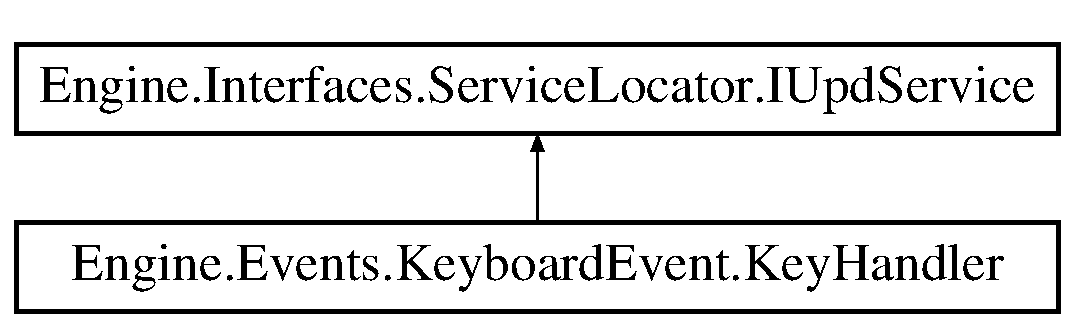
\includegraphics[height=2.000000cm]{d2/d3e/a00366}
\end{center}
\end{figure}
\subsection*{Public Member Functions}
\begin{DoxyCompactItemize}
\item 
delegate void \hyperlink{a00366_a0052951197567196fd40ae4d5e7784e1}{Key\+Event\+Handler} (object sender, \hyperlink{a00362}{Key\+Event\+Args} e)
\item 
void \hyperlink{a00366_a9eb55c55451fa39922f71469f18683ab}{Update} (Game\+Time game\+Time)
\begin{DoxyCompactList}\small\item\em M\+E\+T\+H\+OD\+: The update loop which is cycled through ever frame \end{DoxyCompactList}\end{DoxyCompactItemize}
\subsection*{Protected Member Functions}
\begin{DoxyCompactItemize}
\item 
virtual void \hyperlink{a00366_ae48bbad49979b54cfceebbad82dc48c6}{On\+Key\+Pressed} (Keyboard\+State m, Keys k)
\item 
virtual void \hyperlink{a00366_a8c5bdbe22012f4f6e7febca2c29ec880}{On\+Key\+Held} (Keyboard\+State m, Keys k)
\end{DoxyCompactItemize}
\subsection*{Properties}
\begin{DoxyCompactItemize}
\item 
static \hyperlink{a00366}{Key\+Handler} \hyperlink{a00366_aea9bfd0943bceab24b1632de25df035a}{Instance}\hspace{0.3cm}{\ttfamily  \mbox{[}get\mbox{]}}
\end{DoxyCompactItemize}
\subsection*{Events}
\begin{DoxyCompactItemize}
\item 
\hyperlink{a00366_a0052951197567196fd40ae4d5e7784e1}{Key\+Event\+Handler} \hyperlink{a00366_a71d157bc95a647a5605b9a51e4eab6ea}{Key\+Down}
\item 
\hyperlink{a00366_a0052951197567196fd40ae4d5e7784e1}{Key\+Event\+Handler} \hyperlink{a00366_a8994ba327c6d3f3db097a0308f8ced78}{Key\+Held}
\end{DoxyCompactItemize}


\subsection{Member Function Documentation}
\mbox{\Hypertarget{a00366_a0052951197567196fd40ae4d5e7784e1}\label{a00366_a0052951197567196fd40ae4d5e7784e1}} 
\index{Engine\+::\+Events\+::\+Keyboard\+Event\+::\+Key\+Handler@{Engine\+::\+Events\+::\+Keyboard\+Event\+::\+Key\+Handler}!Key\+Event\+Handler@{Key\+Event\+Handler}}
\index{Key\+Event\+Handler@{Key\+Event\+Handler}!Engine\+::\+Events\+::\+Keyboard\+Event\+::\+Key\+Handler@{Engine\+::\+Events\+::\+Keyboard\+Event\+::\+Key\+Handler}}
\subsubsection{\texorpdfstring{Key\+Event\+Handler()}{KeyEventHandler()}}
{\footnotesize\ttfamily delegate void Engine.\+Events.\+Keyboard\+Event.\+Key\+Handler.\+Key\+Event\+Handler (\begin{DoxyParamCaption}\item[{object}]{sender,  }\item[{\hyperlink{a00362}{Key\+Event\+Args}}]{e }\end{DoxyParamCaption})}

\mbox{\Hypertarget{a00366_a8c5bdbe22012f4f6e7febca2c29ec880}\label{a00366_a8c5bdbe22012f4f6e7febca2c29ec880}} 
\index{Engine\+::\+Events\+::\+Keyboard\+Event\+::\+Key\+Handler@{Engine\+::\+Events\+::\+Keyboard\+Event\+::\+Key\+Handler}!On\+Key\+Held@{On\+Key\+Held}}
\index{On\+Key\+Held@{On\+Key\+Held}!Engine\+::\+Events\+::\+Keyboard\+Event\+::\+Key\+Handler@{Engine\+::\+Events\+::\+Keyboard\+Event\+::\+Key\+Handler}}
\subsubsection{\texorpdfstring{On\+Key\+Held()}{OnKeyHeld()}}
{\footnotesize\ttfamily virtual void Engine.\+Events.\+Keyboard\+Event.\+Key\+Handler.\+On\+Key\+Held (\begin{DoxyParamCaption}\item[{Keyboard\+State}]{m,  }\item[{Keys}]{k }\end{DoxyParamCaption})\hspace{0.3cm}{\ttfamily [inline]}, {\ttfamily [protected]}, {\ttfamily [virtual]}}

\mbox{\Hypertarget{a00366_ae48bbad49979b54cfceebbad82dc48c6}\label{a00366_ae48bbad49979b54cfceebbad82dc48c6}} 
\index{Engine\+::\+Events\+::\+Keyboard\+Event\+::\+Key\+Handler@{Engine\+::\+Events\+::\+Keyboard\+Event\+::\+Key\+Handler}!On\+Key\+Pressed@{On\+Key\+Pressed}}
\index{On\+Key\+Pressed@{On\+Key\+Pressed}!Engine\+::\+Events\+::\+Keyboard\+Event\+::\+Key\+Handler@{Engine\+::\+Events\+::\+Keyboard\+Event\+::\+Key\+Handler}}
\subsubsection{\texorpdfstring{On\+Key\+Pressed()}{OnKeyPressed()}}
{\footnotesize\ttfamily virtual void Engine.\+Events.\+Keyboard\+Event.\+Key\+Handler.\+On\+Key\+Pressed (\begin{DoxyParamCaption}\item[{Keyboard\+State}]{m,  }\item[{Keys}]{k }\end{DoxyParamCaption})\hspace{0.3cm}{\ttfamily [inline]}, {\ttfamily [protected]}, {\ttfamily [virtual]}}

\mbox{\Hypertarget{a00366_a9eb55c55451fa39922f71469f18683ab}\label{a00366_a9eb55c55451fa39922f71469f18683ab}} 
\index{Engine\+::\+Events\+::\+Keyboard\+Event\+::\+Key\+Handler@{Engine\+::\+Events\+::\+Keyboard\+Event\+::\+Key\+Handler}!Update@{Update}}
\index{Update@{Update}!Engine\+::\+Events\+::\+Keyboard\+Event\+::\+Key\+Handler@{Engine\+::\+Events\+::\+Keyboard\+Event\+::\+Key\+Handler}}
\subsubsection{\texorpdfstring{Update()}{Update()}}
{\footnotesize\ttfamily void Engine.\+Events.\+Keyboard\+Event.\+Key\+Handler.\+Update (\begin{DoxyParamCaption}\item[{Game\+Time}]{game\+Time }\end{DoxyParamCaption})\hspace{0.3cm}{\ttfamily [inline]}}



M\+E\+T\+H\+OD\+: The update loop which is cycled through ever frame 


\begin{DoxyParams}{Parameters}
{\em game\+Time} & The Mono\+Game Gametime property\\
\hline
\end{DoxyParams}


Implements \hyperlink{a00478_a387fce2a5440a4dc63f8d72772ecbdaa}{Engine.\+Interfaces.\+Service\+Locator.\+I\+Upd\+Service}.



\subsection{Property Documentation}
\mbox{\Hypertarget{a00366_aea9bfd0943bceab24b1632de25df035a}\label{a00366_aea9bfd0943bceab24b1632de25df035a}} 
\index{Engine\+::\+Events\+::\+Keyboard\+Event\+::\+Key\+Handler@{Engine\+::\+Events\+::\+Keyboard\+Event\+::\+Key\+Handler}!Instance@{Instance}}
\index{Instance@{Instance}!Engine\+::\+Events\+::\+Keyboard\+Event\+::\+Key\+Handler@{Engine\+::\+Events\+::\+Keyboard\+Event\+::\+Key\+Handler}}
\subsubsection{\texorpdfstring{Instance}{Instance}}
{\footnotesize\ttfamily \hyperlink{a00366}{Key\+Handler} Engine.\+Events.\+Keyboard\+Event.\+Key\+Handler.\+Instance\hspace{0.3cm}{\ttfamily [static]}, {\ttfamily [get]}}



\subsection{Event Documentation}
\mbox{\Hypertarget{a00366_a71d157bc95a647a5605b9a51e4eab6ea}\label{a00366_a71d157bc95a647a5605b9a51e4eab6ea}} 
\index{Engine\+::\+Events\+::\+Keyboard\+Event\+::\+Key\+Handler@{Engine\+::\+Events\+::\+Keyboard\+Event\+::\+Key\+Handler}!Key\+Down@{Key\+Down}}
\index{Key\+Down@{Key\+Down}!Engine\+::\+Events\+::\+Keyboard\+Event\+::\+Key\+Handler@{Engine\+::\+Events\+::\+Keyboard\+Event\+::\+Key\+Handler}}
\subsubsection{\texorpdfstring{Key\+Down}{KeyDown}}
{\footnotesize\ttfamily \hyperlink{a00366_a0052951197567196fd40ae4d5e7784e1}{Key\+Event\+Handler} Engine.\+Events.\+Keyboard\+Event.\+Key\+Handler.\+Key\+Down}

\mbox{\Hypertarget{a00366_a8994ba327c6d3f3db097a0308f8ced78}\label{a00366_a8994ba327c6d3f3db097a0308f8ced78}} 
\index{Engine\+::\+Events\+::\+Keyboard\+Event\+::\+Key\+Handler@{Engine\+::\+Events\+::\+Keyboard\+Event\+::\+Key\+Handler}!Key\+Held@{Key\+Held}}
\index{Key\+Held@{Key\+Held}!Engine\+::\+Events\+::\+Keyboard\+Event\+::\+Key\+Handler@{Engine\+::\+Events\+::\+Keyboard\+Event\+::\+Key\+Handler}}
\subsubsection{\texorpdfstring{Key\+Held}{KeyHeld}}
{\footnotesize\ttfamily \hyperlink{a00366_a0052951197567196fd40ae4d5e7784e1}{Key\+Event\+Handler} Engine.\+Events.\+Keyboard\+Event.\+Key\+Handler.\+Key\+Held}



The documentation for this class was generated from the following file\+:\begin{DoxyCompactItemize}
\item 
\hyperlink{a00056}{Key\+Handler.\+cs}\end{DoxyCompactItemize}

\hypertarget{a00370}{}\section{Engine.\+Events.\+Keyboard\+Event.\+Key\+Listener Class Reference}
\label{a00370}\index{Engine.\+Events.\+Keyboard\+Event.\+Key\+Listener@{Engine.\+Events.\+Keyboard\+Event.\+Key\+Listener}}
\subsection*{Public Member Functions}
\begin{DoxyCompactItemize}
\item 
void \hyperlink{a00370_a3de90f1e3196711132154718c47201ff}{On\+Key\+Down} (object sender, \hyperlink{a00362}{Key\+Event\+Args} e)
\end{DoxyCompactItemize}


\subsection{Member Function Documentation}
\mbox{\Hypertarget{a00370_a3de90f1e3196711132154718c47201ff}\label{a00370_a3de90f1e3196711132154718c47201ff}} 
\index{Engine\+::\+Events\+::\+Keyboard\+Event\+::\+Key\+Listener@{Engine\+::\+Events\+::\+Keyboard\+Event\+::\+Key\+Listener}!On\+Key\+Down@{On\+Key\+Down}}
\index{On\+Key\+Down@{On\+Key\+Down}!Engine\+::\+Events\+::\+Keyboard\+Event\+::\+Key\+Listener@{Engine\+::\+Events\+::\+Keyboard\+Event\+::\+Key\+Listener}}
\subsubsection{\texorpdfstring{On\+Key\+Down()}{OnKeyDown()}}
{\footnotesize\ttfamily void Engine.\+Events.\+Keyboard\+Event.\+Key\+Listener.\+On\+Key\+Down (\begin{DoxyParamCaption}\item[{object}]{sender,  }\item[{\hyperlink{a00362}{Key\+Event\+Args}}]{e }\end{DoxyParamCaption})\hspace{0.3cm}{\ttfamily [inline]}}



The documentation for this class was generated from the following file\+:\begin{DoxyCompactItemize}
\item 
\hyperlink{a00059}{Key\+Listener.\+cs}\end{DoxyCompactItemize}

\hypertarget{a00606}{}\section{Engine.\+Utilities.\+Shapes.\+Line Class Reference}
\label{a00606}\index{Engine.\+Utilities.\+Shapes.\+Line@{Engine.\+Utilities.\+Shapes.\+Line}}
Inheritance diagram for Engine.\+Utilities.\+Shapes.\+Line\+:\begin{figure}[H]
\begin{center}
\leavevmode
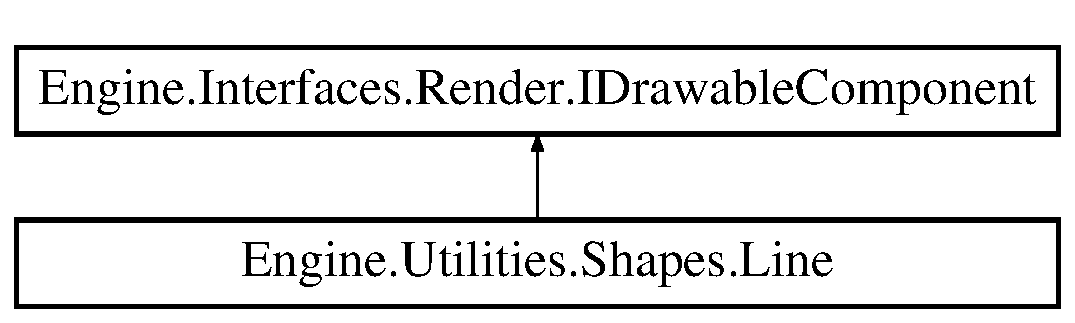
\includegraphics[height=2.000000cm]{d8/d00/a00606}
\end{center}
\end{figure}
\subsection*{Public Member Functions}
\begin{DoxyCompactItemize}
\item 
\hyperlink{a00606_a1697428d93616e1ee1b704f411cc375d}{Line} ()
\item 
void \hyperlink{a00606_a2f3c4a6adefdb08ed78ead11908b2fcb}{new\+Line} (Vector2 start, Vector2 end, Color color)
\item 
void \hyperlink{a00606_a4703c332038f44a1456db6882b6c2b33}{change\+Pos} (Vector2 start, Vector2 end)
\item 
void \hyperlink{a00606_a8500392559da764797cdb92eb850a2ba}{Draw} (Sprite\+Batch spr)
\end{DoxyCompactItemize}
\subsection*{Data Fields}
\begin{DoxyCompactItemize}
\item 
Vector2 \hyperlink{a00606_a0ccdb2e710193d9558ec7a7469365d29}{Start}
\item 
Vector2 \hyperlink{a00606_ab997faeaabf2b56432d38414a60e8f91}{End}
\end{DoxyCompactItemize}


\subsection{Constructor \& Destructor Documentation}
\mbox{\Hypertarget{a00606_a1697428d93616e1ee1b704f411cc375d}\label{a00606_a1697428d93616e1ee1b704f411cc375d}} 
\index{Engine\+::\+Utilities\+::\+Shapes\+::\+Line@{Engine\+::\+Utilities\+::\+Shapes\+::\+Line}!Line@{Line}}
\index{Line@{Line}!Engine\+::\+Utilities\+::\+Shapes\+::\+Line@{Engine\+::\+Utilities\+::\+Shapes\+::\+Line}}
\subsubsection{\texorpdfstring{Line()}{Line()}}
{\footnotesize\ttfamily Engine.\+Utilities.\+Shapes.\+Line.\+Line (\begin{DoxyParamCaption}{ }\end{DoxyParamCaption})\hspace{0.3cm}{\ttfamily [inline]}}



\subsection{Member Function Documentation}
\mbox{\Hypertarget{a00606_a4703c332038f44a1456db6882b6c2b33}\label{a00606_a4703c332038f44a1456db6882b6c2b33}} 
\index{Engine\+::\+Utilities\+::\+Shapes\+::\+Line@{Engine\+::\+Utilities\+::\+Shapes\+::\+Line}!change\+Pos@{change\+Pos}}
\index{change\+Pos@{change\+Pos}!Engine\+::\+Utilities\+::\+Shapes\+::\+Line@{Engine\+::\+Utilities\+::\+Shapes\+::\+Line}}
\subsubsection{\texorpdfstring{change\+Pos()}{changePos()}}
{\footnotesize\ttfamily void Engine.\+Utilities.\+Shapes.\+Line.\+change\+Pos (\begin{DoxyParamCaption}\item[{Vector2}]{start,  }\item[{Vector2}]{end }\end{DoxyParamCaption})\hspace{0.3cm}{\ttfamily [inline]}}

\mbox{\Hypertarget{a00606_a8500392559da764797cdb92eb850a2ba}\label{a00606_a8500392559da764797cdb92eb850a2ba}} 
\index{Engine\+::\+Utilities\+::\+Shapes\+::\+Line@{Engine\+::\+Utilities\+::\+Shapes\+::\+Line}!Draw@{Draw}}
\index{Draw@{Draw}!Engine\+::\+Utilities\+::\+Shapes\+::\+Line@{Engine\+::\+Utilities\+::\+Shapes\+::\+Line}}
\subsubsection{\texorpdfstring{Draw()}{Draw()}}
{\footnotesize\ttfamily void Engine.\+Utilities.\+Shapes.\+Line.\+Draw (\begin{DoxyParamCaption}\item[{Sprite\+Batch}]{spr }\end{DoxyParamCaption})\hspace{0.3cm}{\ttfamily [inline]}}



Implements \hyperlink{a00454_a13aad31e3e179532915dbb93e91afaa3}{Engine.\+Interfaces.\+Render.\+I\+Drawable\+Component}.

\mbox{\Hypertarget{a00606_a2f3c4a6adefdb08ed78ead11908b2fcb}\label{a00606_a2f3c4a6adefdb08ed78ead11908b2fcb}} 
\index{Engine\+::\+Utilities\+::\+Shapes\+::\+Line@{Engine\+::\+Utilities\+::\+Shapes\+::\+Line}!new\+Line@{new\+Line}}
\index{new\+Line@{new\+Line}!Engine\+::\+Utilities\+::\+Shapes\+::\+Line@{Engine\+::\+Utilities\+::\+Shapes\+::\+Line}}
\subsubsection{\texorpdfstring{new\+Line()}{newLine()}}
{\footnotesize\ttfamily void Engine.\+Utilities.\+Shapes.\+Line.\+new\+Line (\begin{DoxyParamCaption}\item[{Vector2}]{start,  }\item[{Vector2}]{end,  }\item[{Color}]{color }\end{DoxyParamCaption})\hspace{0.3cm}{\ttfamily [inline]}}



\subsection{Field Documentation}
\mbox{\Hypertarget{a00606_ab997faeaabf2b56432d38414a60e8f91}\label{a00606_ab997faeaabf2b56432d38414a60e8f91}} 
\index{Engine\+::\+Utilities\+::\+Shapes\+::\+Line@{Engine\+::\+Utilities\+::\+Shapes\+::\+Line}!End@{End}}
\index{End@{End}!Engine\+::\+Utilities\+::\+Shapes\+::\+Line@{Engine\+::\+Utilities\+::\+Shapes\+::\+Line}}
\subsubsection{\texorpdfstring{End}{End}}
{\footnotesize\ttfamily Vector2 Engine.\+Utilities.\+Shapes.\+Line.\+End}

\mbox{\Hypertarget{a00606_a0ccdb2e710193d9558ec7a7469365d29}\label{a00606_a0ccdb2e710193d9558ec7a7469365d29}} 
\index{Engine\+::\+Utilities\+::\+Shapes\+::\+Line@{Engine\+::\+Utilities\+::\+Shapes\+::\+Line}!Start@{Start}}
\index{Start@{Start}!Engine\+::\+Utilities\+::\+Shapes\+::\+Line@{Engine\+::\+Utilities\+::\+Shapes\+::\+Line}}
\subsubsection{\texorpdfstring{Start}{Start}}
{\footnotesize\ttfamily Vector2 Engine.\+Utilities.\+Shapes.\+Line.\+Start}



The documentation for this class was generated from the following file\+:\begin{DoxyCompactItemize}
\item 
\hyperlink{a00236}{Line.\+cs}\end{DoxyCompactItemize}

\hypertarget{a00542}{}\section{Engine.\+Managers.\+Service\+Locator.\+Locator Class Reference}
\label{a00542}\index{Engine.\+Managers.\+Service\+Locator.\+Locator@{Engine.\+Managers.\+Service\+Locator.\+Locator}}


C\+L\+A\+SS\+: A service locator that removes the need for each manager to be a singleton. This is now the only Singleton required in the whole program. It allows us to access each manager and call the method from each Manager as we require it  


Inheritance diagram for Engine.\+Managers.\+Service\+Locator.\+Locator\+:\begin{figure}[H]
\begin{center}
\leavevmode
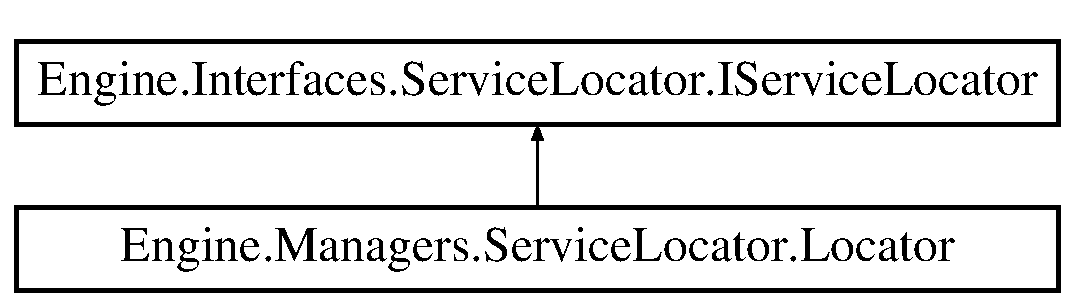
\includegraphics[height=2.000000cm]{d0/ddb/a00542}
\end{center}
\end{figure}
\subsection*{Public Member Functions}
\begin{DoxyCompactItemize}
\item 
void \hyperlink{a00542_a34bc6f5d735512bae556d2ec65a7bda7}{Initialize\+Services} (Content\+Manager c, Sprite\+Batch sb)
\begin{DoxyCompactList}\small\item\em M\+E\+T\+H\+OD\+: Initialises each service for the program to run \end{DoxyCompactList}\item 
T \hyperlink{a00542_a2bb3c0174bd67904d148bc789c9faaba}{get\+Service$<$ T $>$} ()
\begin{DoxyCompactList}\small\item\em M\+E\+T\+H\+OD\+: Gets and returns a service of the generic type input in the parameter \end{DoxyCompactList}\item 
void \hyperlink{a00542_a2a2ead2e1ed9a2d63b59ab34621b0812}{register\+Service$<$ T $>$} (T val)
\begin{DoxyCompactList}\small\item\em M\+E\+T\+H\+OD\+: Register the service and check whether it needs to be updated \end{DoxyCompactList}\item 
void \hyperlink{a00542_af5c3ce0526940dffc81919b2ef35d652}{register\+U\+P\+D\+Service$<$ T $>$} (T val)
\begin{DoxyCompactList}\small\item\em M\+E\+T\+H\+OD\+: Register Update service \end{DoxyCompactList}\item 
void \hyperlink{a00542_ab66a423db26d79e6fc655df699a64f0c}{Update\+Services} (Game\+Time game\+Time)
\begin{DoxyCompactList}\small\item\em M\+E\+T\+H\+OD\+: Update all services that require it \end{DoxyCompactList}\end{DoxyCompactItemize}
\subsection*{Properties}
\begin{DoxyCompactItemize}
\item 
static \hyperlink{a00542}{Locator} \hyperlink{a00542_ab1da0b54c482b49d1654f9763b161883}{Instance}\hspace{0.3cm}{\ttfamily  \mbox{[}get\mbox{]}}
\begin{DoxyCompactList}\small\item\em S\+I\+N\+G\+L\+E\+T\+ON \end{DoxyCompactList}\end{DoxyCompactItemize}


\subsection{Detailed Description}
C\+L\+A\+SS\+: A service locator that removes the need for each manager to be a singleton. This is now the only Singleton required in the whole program. It allows us to access each manager and call the method from each Manager as we require it 



\subsection{Member Function Documentation}
\mbox{\Hypertarget{a00542_a2bb3c0174bd67904d148bc789c9faaba}\label{a00542_a2bb3c0174bd67904d148bc789c9faaba}} 
\index{Engine\+::\+Managers\+::\+Service\+Locator\+::\+Locator@{Engine\+::\+Managers\+::\+Service\+Locator\+::\+Locator}!get\+Service$<$ T $>$@{get\+Service$<$ T $>$}}
\index{get\+Service$<$ T $>$@{get\+Service$<$ T $>$}!Engine\+::\+Managers\+::\+Service\+Locator\+::\+Locator@{Engine\+::\+Managers\+::\+Service\+Locator\+::\+Locator}}
\subsubsection{\texorpdfstring{get\+Service$<$ T $>$()}{getService< T >()}}
{\footnotesize\ttfamily T Engine.\+Managers.\+Service\+Locator.\+Locator.\+get\+Service$<$ T $>$ (\begin{DoxyParamCaption}{ }\end{DoxyParamCaption})\hspace{0.3cm}{\ttfamily [inline]}}



M\+E\+T\+H\+OD\+: Gets and returns a service of the generic type input in the parameter 


\begin{DoxyTemplParams}{Template Parameters}
{\em T} & Generic type T of the service to be requested\\
\hline
\end{DoxyTemplParams}
\begin{DoxyReturn}{Returns}
Service of Type T
\end{DoxyReturn}
T\+RY\+: to return the service from the hashmap

T\+RY\+: to catch a null reference exception 

Implements \hyperlink{a00474_a39ce84b8fb97655fd7039be3c4fa5f1c}{Engine.\+Interfaces.\+Service\+Locator.\+I\+Service\+Locator}.

\mbox{\Hypertarget{a00542_a34bc6f5d735512bae556d2ec65a7bda7}\label{a00542_a34bc6f5d735512bae556d2ec65a7bda7}} 
\index{Engine\+::\+Managers\+::\+Service\+Locator\+::\+Locator@{Engine\+::\+Managers\+::\+Service\+Locator\+::\+Locator}!Initialize\+Services@{Initialize\+Services}}
\index{Initialize\+Services@{Initialize\+Services}!Engine\+::\+Managers\+::\+Service\+Locator\+::\+Locator@{Engine\+::\+Managers\+::\+Service\+Locator\+::\+Locator}}
\subsubsection{\texorpdfstring{Initialize\+Services()}{InitializeServices()}}
{\footnotesize\ttfamily void Engine.\+Managers.\+Service\+Locator.\+Locator.\+Initialize\+Services (\begin{DoxyParamCaption}\item[{Content\+Manager}]{c,  }\item[{Sprite\+Batch}]{sb }\end{DoxyParamCaption})\hspace{0.3cm}{\ttfamily [inline]}}



M\+E\+T\+H\+OD\+: Initialises each service for the program to run 


\begin{DoxyParams}{Parameters}
{\em c} & the monogame Content\+Manager to be used\\
\hline
{\em sb} & the monogame sprite\+Batch to be used\\
\hline
\end{DoxyParams}
Mouse and Keyboard Handlers

\hyperlink{a00266}{Behaviour} Manager

Camera Manager

sound Manager

\hyperlink{a00272}{Resource} Loader

Entity Manager

\hyperlink{a00266}{Behaviour} Manager

\hyperlink{a00268}{Collision} Manager

\hyperlink{a00271}{Render} Manager

\hyperlink{a00273}{Screen} Manager 

Implements \hyperlink{a00474_a4bf9f6979adf99eda26320a420262991}{Engine.\+Interfaces.\+Service\+Locator.\+I\+Service\+Locator}.

\mbox{\Hypertarget{a00542_a2a2ead2e1ed9a2d63b59ab34621b0812}\label{a00542_a2a2ead2e1ed9a2d63b59ab34621b0812}} 
\index{Engine\+::\+Managers\+::\+Service\+Locator\+::\+Locator@{Engine\+::\+Managers\+::\+Service\+Locator\+::\+Locator}!register\+Service$<$ T $>$@{register\+Service$<$ T $>$}}
\index{register\+Service$<$ T $>$@{register\+Service$<$ T $>$}!Engine\+::\+Managers\+::\+Service\+Locator\+::\+Locator@{Engine\+::\+Managers\+::\+Service\+Locator\+::\+Locator}}
\subsubsection{\texorpdfstring{register\+Service$<$ T $>$()}{registerService< T >()}}
{\footnotesize\ttfamily void Engine.\+Managers.\+Service\+Locator.\+Locator.\+register\+Service$<$ T $>$ (\begin{DoxyParamCaption}\item[{T}]{val }\end{DoxyParamCaption})\hspace{0.3cm}{\ttfamily [inline]}}



M\+E\+T\+H\+OD\+: Register the service and check whether it needs to be updated 


\begin{DoxyTemplParams}{Template Parameters}
{\em T} & Generic service\\
\hline
\end{DoxyTemplParams}

\begin{DoxyParams}{Parameters}
{\em val} & Service of Type T\\
\hline
\end{DoxyParams}
T\+RY\+:

IF\+: val parameter is not null and is in the \+\_\+services Dictionary

A\+DD\+: Service to the dictionary

C\+A\+T\+CH\+: Exception

T\+H\+R\+OW\+: Argument exception \mbox{\Hypertarget{a00542_af5c3ce0526940dffc81919b2ef35d652}\label{a00542_af5c3ce0526940dffc81919b2ef35d652}} 
\index{Engine\+::\+Managers\+::\+Service\+Locator\+::\+Locator@{Engine\+::\+Managers\+::\+Service\+Locator\+::\+Locator}!register\+U\+P\+D\+Service$<$ T $>$@{register\+U\+P\+D\+Service$<$ T $>$}}
\index{register\+U\+P\+D\+Service$<$ T $>$@{register\+U\+P\+D\+Service$<$ T $>$}!Engine\+::\+Managers\+::\+Service\+Locator\+::\+Locator@{Engine\+::\+Managers\+::\+Service\+Locator\+::\+Locator}}
\subsubsection{\texorpdfstring{register\+U\+P\+D\+Service$<$ T $>$()}{registerUPDService< T >()}}
{\footnotesize\ttfamily void Engine.\+Managers.\+Service\+Locator.\+Locator.\+register\+U\+P\+D\+Service$<$ T $>$ (\begin{DoxyParamCaption}\item[{T}]{val }\end{DoxyParamCaption})\hspace{0.3cm}{\ttfamily [inline]}}



M\+E\+T\+H\+OD\+: Register Update service 


\begin{DoxyTemplParams}{Template Parameters}
{\em T} & \\
\hline
\end{DoxyTemplParams}

\begin{DoxyParams}{Parameters}
{\em val} & \\
\hline
\end{DoxyParams}
\mbox{\Hypertarget{a00542_ab66a423db26d79e6fc655df699a64f0c}\label{a00542_ab66a423db26d79e6fc655df699a64f0c}} 
\index{Engine\+::\+Managers\+::\+Service\+Locator\+::\+Locator@{Engine\+::\+Managers\+::\+Service\+Locator\+::\+Locator}!Update\+Services@{Update\+Services}}
\index{Update\+Services@{Update\+Services}!Engine\+::\+Managers\+::\+Service\+Locator\+::\+Locator@{Engine\+::\+Managers\+::\+Service\+Locator\+::\+Locator}}
\subsubsection{\texorpdfstring{Update\+Services()}{UpdateServices()}}
{\footnotesize\ttfamily void Engine.\+Managers.\+Service\+Locator.\+Locator.\+Update\+Services (\begin{DoxyParamCaption}\item[{Game\+Time}]{game\+Time }\end{DoxyParamCaption})\hspace{0.3cm}{\ttfamily [inline]}}



M\+E\+T\+H\+OD\+: Update all services that require it 


\begin{DoxyParams}{Parameters}
{\em game\+Time} & \\
\hline
\end{DoxyParams}


Implements \hyperlink{a00474_a5bf3aab2adcf14c813a348325003ddcc}{Engine.\+Interfaces.\+Service\+Locator.\+I\+Service\+Locator}.



\subsection{Property Documentation}
\mbox{\Hypertarget{a00542_ab1da0b54c482b49d1654f9763b161883}\label{a00542_ab1da0b54c482b49d1654f9763b161883}} 
\index{Engine\+::\+Managers\+::\+Service\+Locator\+::\+Locator@{Engine\+::\+Managers\+::\+Service\+Locator\+::\+Locator}!Instance@{Instance}}
\index{Instance@{Instance}!Engine\+::\+Managers\+::\+Service\+Locator\+::\+Locator@{Engine\+::\+Managers\+::\+Service\+Locator\+::\+Locator}}
\subsubsection{\texorpdfstring{Instance}{Instance}}
{\footnotesize\ttfamily \hyperlink{a00542}{Locator} Engine.\+Managers.\+Service\+Locator.\+Locator.\+Instance\hspace{0.3cm}{\ttfamily [static]}, {\ttfamily [get]}}



S\+I\+N\+G\+L\+E\+T\+ON 



The documentation for this class was generated from the following file\+:\begin{DoxyCompactItemize}
\item 
\hyperlink{a00188}{Locator.\+cs}\end{DoxyCompactItemize}

\hypertarget{a00574}{}\section{Engine.\+States.\+Menu.\+Main\+Menu Class Reference}
\label{a00574}\index{Engine.\+States.\+Menu.\+Main\+Menu@{Engine.\+States.\+Menu.\+Main\+Menu}}


C\+L\+A\+SS\+: \hyperlink{a00574}{Main\+Menu}, this is the class that is loaded straight after the splash screen is used to access the majority of other screens in the program  


Inheritance diagram for Engine.\+States.\+Menu.\+Main\+Menu\+:\begin{figure}[H]
\begin{center}
\leavevmode
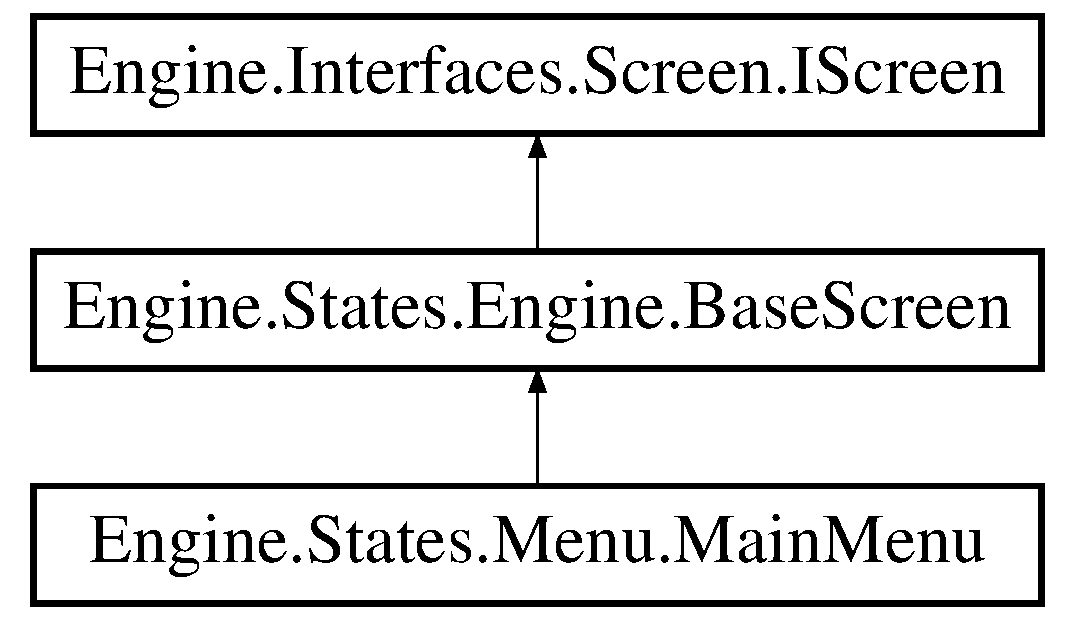
\includegraphics[height=3.000000cm]{d4/dbe/a00574}
\end{center}
\end{figure}
\subsection*{Public Member Functions}
\begin{DoxyCompactItemize}
\item 
\hyperlink{a00574_a90df30106a466b9da59ebda89c6172db}{Main\+Menu} ()
\item 
override void \hyperlink{a00574_a43b83f0941e721234fdceeb0b5587f1b}{Initialize} ()
\begin{DoxyCompactList}\small\item\em M\+E\+T\+H\+OD\+: Initialises the logic of the screen \end{DoxyCompactList}\item 
override void \hyperlink{a00574_a193970cc59914f538ae0bcd39fe1ef48}{Draw} (Sprite\+Batch sprite\+Batch)
\begin{DoxyCompactList}\small\item\em M\+E\+T\+H\+OD\+: Draws the content of the screen \end{DoxyCompactList}\item 
override void \hyperlink{a00574_ad667a7ff9dea79bee26a4205418c7a61}{Update} (Game\+Time game\+Time)
\begin{DoxyCompactList}\small\item\em M\+E\+T\+H\+OD\+: The update loop which is cycled through each frame \end{DoxyCompactList}\item 
void \hyperlink{a00574_a18a59c1bc70e322805c36a3ca5c7d107}{Check\+Limits} ()
\item 
void \hyperlink{a00574_acb1e589815e4a3897d061d69a17dd7d9}{On\+Key\+Down} (object sender, \hyperlink{a00362}{Key\+Event\+Args} e)
\item 
void \hyperlink{a00574_a3f150b2f6278d7267d54b38601534ed1}{Menu\+Selection} ()
\end{DoxyCompactItemize}
\subsection*{Additional Inherited Members}


\subsection{Detailed Description}
C\+L\+A\+SS\+: \hyperlink{a00574}{Main\+Menu}, this is the class that is loaded straight after the splash screen is used to access the majority of other screens in the program 



\subsection{Constructor \& Destructor Documentation}
\mbox{\Hypertarget{a00574_a90df30106a466b9da59ebda89c6172db}\label{a00574_a90df30106a466b9da59ebda89c6172db}} 
\index{Engine\+::\+States\+::\+Menu\+::\+Main\+Menu@{Engine\+::\+States\+::\+Menu\+::\+Main\+Menu}!Main\+Menu@{Main\+Menu}}
\index{Main\+Menu@{Main\+Menu}!Engine\+::\+States\+::\+Menu\+::\+Main\+Menu@{Engine\+::\+States\+::\+Menu\+::\+Main\+Menu}}
\subsubsection{\texorpdfstring{Main\+Menu()}{MainMenu()}}
{\footnotesize\ttfamily Engine.\+States.\+Menu.\+Main\+Menu.\+Main\+Menu (\begin{DoxyParamCaption}{ }\end{DoxyParamCaption})\hspace{0.3cm}{\ttfamily [inline]}}



\subsection{Member Function Documentation}
\mbox{\Hypertarget{a00574_a18a59c1bc70e322805c36a3ca5c7d107}\label{a00574_a18a59c1bc70e322805c36a3ca5c7d107}} 
\index{Engine\+::\+States\+::\+Menu\+::\+Main\+Menu@{Engine\+::\+States\+::\+Menu\+::\+Main\+Menu}!Check\+Limits@{Check\+Limits}}
\index{Check\+Limits@{Check\+Limits}!Engine\+::\+States\+::\+Menu\+::\+Main\+Menu@{Engine\+::\+States\+::\+Menu\+::\+Main\+Menu}}
\subsubsection{\texorpdfstring{Check\+Limits()}{CheckLimits()}}
{\footnotesize\ttfamily void Engine.\+States.\+Menu.\+Main\+Menu.\+Check\+Limits (\begin{DoxyParamCaption}{ }\end{DoxyParamCaption})\hspace{0.3cm}{\ttfamily [inline]}}

\mbox{\Hypertarget{a00574_a193970cc59914f538ae0bcd39fe1ef48}\label{a00574_a193970cc59914f538ae0bcd39fe1ef48}} 
\index{Engine\+::\+States\+::\+Menu\+::\+Main\+Menu@{Engine\+::\+States\+::\+Menu\+::\+Main\+Menu}!Draw@{Draw}}
\index{Draw@{Draw}!Engine\+::\+States\+::\+Menu\+::\+Main\+Menu@{Engine\+::\+States\+::\+Menu\+::\+Main\+Menu}}
\subsubsection{\texorpdfstring{Draw()}{Draw()}}
{\footnotesize\ttfamily override void Engine.\+States.\+Menu.\+Main\+Menu.\+Draw (\begin{DoxyParamCaption}\item[{Sprite\+Batch}]{sprite\+Batch }\end{DoxyParamCaption})\hspace{0.3cm}{\ttfamily [inline]}, {\ttfamily [virtual]}}



M\+E\+T\+H\+OD\+: Draws the content of the screen 


\begin{DoxyParams}{Parameters}
{\em sprite\+Batch} & the Monogame Sprite\+Batch\\
\hline
\end{DoxyParams}


Reimplemented from \hyperlink{a00550_a200c31954effe5fc060118607155fb16}{Engine.\+States.\+Engine.\+Base\+Screen}.

\mbox{\Hypertarget{a00574_a43b83f0941e721234fdceeb0b5587f1b}\label{a00574_a43b83f0941e721234fdceeb0b5587f1b}} 
\index{Engine\+::\+States\+::\+Menu\+::\+Main\+Menu@{Engine\+::\+States\+::\+Menu\+::\+Main\+Menu}!Initialize@{Initialize}}
\index{Initialize@{Initialize}!Engine\+::\+States\+::\+Menu\+::\+Main\+Menu@{Engine\+::\+States\+::\+Menu\+::\+Main\+Menu}}
\subsubsection{\texorpdfstring{Initialize()}{Initialize()}}
{\footnotesize\ttfamily override void Engine.\+States.\+Menu.\+Main\+Menu.\+Initialize (\begin{DoxyParamCaption}{ }\end{DoxyParamCaption})\hspace{0.3cm}{\ttfamily [inline]}, {\ttfamily [virtual]}}



M\+E\+T\+H\+OD\+: Initialises the logic of the screen 

I\+N\+I\+T\+I\+A\+L\+I\+SE\+: The fader D\+E\+C\+L\+A\+R\+ED earlier

S\+ET\+: Soundtrack

E\+V\+E\+NT\+: Add Keydown event to the screen

A\+DD\+: Different possible selections to the menu

F\+OR\+: Each item in the Menu\+Names\+: Move down the screen and draw the strings 

Reimplemented from \hyperlink{a00550_af8fd6890abf865641e190578ef2e054c}{Engine.\+States.\+Engine.\+Base\+Screen}.

\mbox{\Hypertarget{a00574_a3f150b2f6278d7267d54b38601534ed1}\label{a00574_a3f150b2f6278d7267d54b38601534ed1}} 
\index{Engine\+::\+States\+::\+Menu\+::\+Main\+Menu@{Engine\+::\+States\+::\+Menu\+::\+Main\+Menu}!Menu\+Selection@{Menu\+Selection}}
\index{Menu\+Selection@{Menu\+Selection}!Engine\+::\+States\+::\+Menu\+::\+Main\+Menu@{Engine\+::\+States\+::\+Menu\+::\+Main\+Menu}}
\subsubsection{\texorpdfstring{Menu\+Selection()}{MenuSelection()}}
{\footnotesize\ttfamily void Engine.\+States.\+Menu.\+Main\+Menu.\+Menu\+Selection (\begin{DoxyParamCaption}{ }\end{DoxyParamCaption})\hspace{0.3cm}{\ttfamily [inline]}}

\mbox{\Hypertarget{a00574_acb1e589815e4a3897d061d69a17dd7d9}\label{a00574_acb1e589815e4a3897d061d69a17dd7d9}} 
\index{Engine\+::\+States\+::\+Menu\+::\+Main\+Menu@{Engine\+::\+States\+::\+Menu\+::\+Main\+Menu}!On\+Key\+Down@{On\+Key\+Down}}
\index{On\+Key\+Down@{On\+Key\+Down}!Engine\+::\+States\+::\+Menu\+::\+Main\+Menu@{Engine\+::\+States\+::\+Menu\+::\+Main\+Menu}}
\subsubsection{\texorpdfstring{On\+Key\+Down()}{OnKeyDown()}}
{\footnotesize\ttfamily void Engine.\+States.\+Menu.\+Main\+Menu.\+On\+Key\+Down (\begin{DoxyParamCaption}\item[{object}]{sender,  }\item[{\hyperlink{a00362}{Key\+Event\+Args}}]{e }\end{DoxyParamCaption})\hspace{0.3cm}{\ttfamily [inline]}}

\mbox{\Hypertarget{a00574_ad667a7ff9dea79bee26a4205418c7a61}\label{a00574_ad667a7ff9dea79bee26a4205418c7a61}} 
\index{Engine\+::\+States\+::\+Menu\+::\+Main\+Menu@{Engine\+::\+States\+::\+Menu\+::\+Main\+Menu}!Update@{Update}}
\index{Update@{Update}!Engine\+::\+States\+::\+Menu\+::\+Main\+Menu@{Engine\+::\+States\+::\+Menu\+::\+Main\+Menu}}
\subsubsection{\texorpdfstring{Update()}{Update()}}
{\footnotesize\ttfamily override void Engine.\+States.\+Menu.\+Main\+Menu.\+Update (\begin{DoxyParamCaption}\item[{Game\+Time}]{game\+Time }\end{DoxyParamCaption})\hspace{0.3cm}{\ttfamily [inline]}, {\ttfamily [virtual]}}



M\+E\+T\+H\+OD\+: The update loop which is cycled through each frame 


\begin{DoxyParams}{Parameters}
{\em game\+Time} & the Monogame Game\+Time property\\
\hline
\end{DoxyParams}


Reimplemented from \hyperlink{a00550_a098ece7d1e112475f6e880c3a672af64}{Engine.\+States.\+Engine.\+Base\+Screen}.



The documentation for this class was generated from the following file\+:\begin{DoxyCompactItemize}
\item 
\hyperlink{a00212}{Main\+Menu.\+cs}\end{DoxyCompactItemize}

\hypertarget{a00578}{}\section{Engine.\+Menu\+Item Class Reference}
\label{a00578}\index{Engine.\+Menu\+Item@{Engine.\+Menu\+Item}}
\subsection*{Public Member Functions}
\begin{DoxyCompactItemize}
\item 
\hyperlink{a00578_af8c1e0084202dd6048beb56c3e8ea1eb}{Menu\+Item} (string \+\_\+name, float y\+Offset, Sprite\+Font \+\_\+sprite\+Font, int \+\_\+index, Texture2D b\+Tex)
\item 
\hyperlink{a00578_a79a905f74d6632e0c8cda3cd951072a2}{Menu\+Item} (string \+\_\+name, float y\+Offset, Sprite\+Font \+\_\+sprite\+Font, int \+\_\+index, Texture2D b\+Tex, float \hyperlink{a00578_a8f2bf7f4310e299f7ef8ff70729c3aff}{scale})
\item 
void \hyperlink{a00578_afdc8061ebe0db94ec3c73c3648f35c27}{Draw} (Sprite\+Batch sprite\+Batch)
\end{DoxyCompactItemize}
\subsection*{Data Fields}
\begin{DoxyCompactItemize}
\item 
Vector2 \hyperlink{a00578_a45b562c09b4b905b48941cc5723265af}{position}
\item 
float \hyperlink{a00578_a8f2bf7f4310e299f7ef8ff70729c3aff}{scale} = 1.\+5f
\end{DoxyCompactItemize}
\subsection*{Properties}
\begin{DoxyCompactItemize}
\item 
bool \hyperlink{a00578_a7455f6df46a7eb219f4c03c7f311fec2}{Is\+Selected}\hspace{0.3cm}{\ttfamily  \mbox{[}get, set\mbox{]}}
\item 
string \hyperlink{a00578_abf3d8b83686d4378d2bb2d5cc2ccbf5a}{Name}\hspace{0.3cm}{\ttfamily  \mbox{[}get, set\mbox{]}}
\item 
int \hyperlink{a00578_a7bef8d2c1b94b0edf19a89cf76269442}{Index}\hspace{0.3cm}{\ttfamily  \mbox{[}get, set\mbox{]}}
\end{DoxyCompactItemize}


\subsection{Constructor \& Destructor Documentation}
\mbox{\Hypertarget{a00578_af8c1e0084202dd6048beb56c3e8ea1eb}\label{a00578_af8c1e0084202dd6048beb56c3e8ea1eb}} 
\index{Engine\+::\+Menu\+Item@{Engine\+::\+Menu\+Item}!Menu\+Item@{Menu\+Item}}
\index{Menu\+Item@{Menu\+Item}!Engine\+::\+Menu\+Item@{Engine\+::\+Menu\+Item}}
\subsubsection{\texorpdfstring{Menu\+Item()}{MenuItem()}\hspace{0.1cm}{\footnotesize\ttfamily [1/2]}}
{\footnotesize\ttfamily Engine.\+Menu\+Item.\+Menu\+Item (\begin{DoxyParamCaption}\item[{string}]{\+\_\+name,  }\item[{float}]{y\+Offset,  }\item[{Sprite\+Font}]{\+\_\+sprite\+Font,  }\item[{int}]{\+\_\+index,  }\item[{Texture2D}]{b\+Tex }\end{DoxyParamCaption})\hspace{0.3cm}{\ttfamily [inline]}}

\mbox{\Hypertarget{a00578_a79a905f74d6632e0c8cda3cd951072a2}\label{a00578_a79a905f74d6632e0c8cda3cd951072a2}} 
\index{Engine\+::\+Menu\+Item@{Engine\+::\+Menu\+Item}!Menu\+Item@{Menu\+Item}}
\index{Menu\+Item@{Menu\+Item}!Engine\+::\+Menu\+Item@{Engine\+::\+Menu\+Item}}
\subsubsection{\texorpdfstring{Menu\+Item()}{MenuItem()}\hspace{0.1cm}{\footnotesize\ttfamily [2/2]}}
{\footnotesize\ttfamily Engine.\+Menu\+Item.\+Menu\+Item (\begin{DoxyParamCaption}\item[{string}]{\+\_\+name,  }\item[{float}]{y\+Offset,  }\item[{Sprite\+Font}]{\+\_\+sprite\+Font,  }\item[{int}]{\+\_\+index,  }\item[{Texture2D}]{b\+Tex,  }\item[{float}]{scale }\end{DoxyParamCaption})\hspace{0.3cm}{\ttfamily [inline]}}



\subsection{Member Function Documentation}
\mbox{\Hypertarget{a00578_afdc8061ebe0db94ec3c73c3648f35c27}\label{a00578_afdc8061ebe0db94ec3c73c3648f35c27}} 
\index{Engine\+::\+Menu\+Item@{Engine\+::\+Menu\+Item}!Draw@{Draw}}
\index{Draw@{Draw}!Engine\+::\+Menu\+Item@{Engine\+::\+Menu\+Item}}
\subsubsection{\texorpdfstring{Draw()}{Draw()}}
{\footnotesize\ttfamily void Engine.\+Menu\+Item.\+Draw (\begin{DoxyParamCaption}\item[{Sprite\+Batch}]{sprite\+Batch }\end{DoxyParamCaption})\hspace{0.3cm}{\ttfamily [inline]}}

sprite\+Batch.\+Draw(button\+Texture, screen\+Center,null, Color.\+White,0f,texture\+Center,1f,Sprite\+Effects.\+None,0.\+5f); 

\subsection{Field Documentation}
\mbox{\Hypertarget{a00578_a45b562c09b4b905b48941cc5723265af}\label{a00578_a45b562c09b4b905b48941cc5723265af}} 
\index{Engine\+::\+Menu\+Item@{Engine\+::\+Menu\+Item}!position@{position}}
\index{position@{position}!Engine\+::\+Menu\+Item@{Engine\+::\+Menu\+Item}}
\subsubsection{\texorpdfstring{position}{position}}
{\footnotesize\ttfamily Vector2 Engine.\+Menu\+Item.\+position}

\mbox{\Hypertarget{a00578_a8f2bf7f4310e299f7ef8ff70729c3aff}\label{a00578_a8f2bf7f4310e299f7ef8ff70729c3aff}} 
\index{Engine\+::\+Menu\+Item@{Engine\+::\+Menu\+Item}!scale@{scale}}
\index{scale@{scale}!Engine\+::\+Menu\+Item@{Engine\+::\+Menu\+Item}}
\subsubsection{\texorpdfstring{scale}{scale}}
{\footnotesize\ttfamily float Engine.\+Menu\+Item.\+scale = 1.\+5f}



\subsection{Property Documentation}
\mbox{\Hypertarget{a00578_a7bef8d2c1b94b0edf19a89cf76269442}\label{a00578_a7bef8d2c1b94b0edf19a89cf76269442}} 
\index{Engine\+::\+Menu\+Item@{Engine\+::\+Menu\+Item}!Index@{Index}}
\index{Index@{Index}!Engine\+::\+Menu\+Item@{Engine\+::\+Menu\+Item}}
\subsubsection{\texorpdfstring{Index}{Index}}
{\footnotesize\ttfamily int Engine.\+Menu\+Item.\+Index\hspace{0.3cm}{\ttfamily [get]}, {\ttfamily [set]}}

\mbox{\Hypertarget{a00578_a7455f6df46a7eb219f4c03c7f311fec2}\label{a00578_a7455f6df46a7eb219f4c03c7f311fec2}} 
\index{Engine\+::\+Menu\+Item@{Engine\+::\+Menu\+Item}!Is\+Selected@{Is\+Selected}}
\index{Is\+Selected@{Is\+Selected}!Engine\+::\+Menu\+Item@{Engine\+::\+Menu\+Item}}
\subsubsection{\texorpdfstring{Is\+Selected}{IsSelected}}
{\footnotesize\ttfamily bool Engine.\+Menu\+Item.\+Is\+Selected\hspace{0.3cm}{\ttfamily [get]}, {\ttfamily [set]}}

\mbox{\Hypertarget{a00578_abf3d8b83686d4378d2bb2d5cc2ccbf5a}\label{a00578_abf3d8b83686d4378d2bb2d5cc2ccbf5a}} 
\index{Engine\+::\+Menu\+Item@{Engine\+::\+Menu\+Item}!Name@{Name}}
\index{Name@{Name}!Engine\+::\+Menu\+Item@{Engine\+::\+Menu\+Item}}
\subsubsection{\texorpdfstring{Name}{Name}}
{\footnotesize\ttfamily string Engine.\+Menu\+Item.\+Name\hspace{0.3cm}{\ttfamily [get]}, {\ttfamily [set]}}



The documentation for this class was generated from the following file\+:\begin{DoxyCompactItemize}
\item 
\hyperlink{a00215}{Menu\+Item.\+cs}\end{DoxyCompactItemize}

\hypertarget{a00582}{}\section{Engine.\+States.\+Menu.\+Menu\+Option Class Reference}
\label{a00582}\index{Engine.\+States.\+Menu.\+Menu\+Option@{Engine.\+States.\+Menu.\+Menu\+Option}}


C\+L\+A\+SS\+: \hyperlink{a00582}{Menu\+Option} contains the data and logic for creating new options to be highlighted on a menu  


\subsection*{Public Member Functions}
\begin{DoxyCompactItemize}
\item 
\hyperlink{a00582_a4a2c68f6b84495780f1cd0b716458204}{Menu\+Option} (string \+\_\+name, float offset, int \+\_\+index)
\begin{DoxyCompactList}\small\item\em C\+O\+N\+S\+T\+R\+U\+C\+T\+OR \end{DoxyCompactList}\item 
void \hyperlink{a00582_a824068f71d00483a40dd293049e2a10f}{Draw} (Sprite\+Batch sprite\+Batch)
\begin{DoxyCompactList}\small\item\em M\+E\+T\+H\+OD\+: Draws the menu Option \end{DoxyCompactList}\end{DoxyCompactItemize}
\subsection*{Properties}
\begin{DoxyCompactItemize}
\item 
bool \hyperlink{a00582_ae71156b6308de01502ec3a6242d6aed2}{Is\+Selected}\hspace{0.3cm}{\ttfamily  \mbox{[}get, set\mbox{]}}
\item 
string \hyperlink{a00582_ae1b8c3d46b2bb4efcffc3c5d95efe6f8}{Name}\hspace{0.3cm}{\ttfamily  \mbox{[}get, set\mbox{]}}
\item 
int \hyperlink{a00582_a378ae17c1e26363dba73e2f5e691fa78}{Index}\hspace{0.3cm}{\ttfamily  \mbox{[}get, set\mbox{]}}
\end{DoxyCompactItemize}


\subsection{Detailed Description}
C\+L\+A\+SS\+: \hyperlink{a00582}{Menu\+Option} contains the data and logic for creating new options to be highlighted on a menu 



\subsection{Constructor \& Destructor Documentation}
\mbox{\Hypertarget{a00582_a4a2c68f6b84495780f1cd0b716458204}\label{a00582_a4a2c68f6b84495780f1cd0b716458204}} 
\index{Engine\+::\+States\+::\+Menu\+::\+Menu\+Option@{Engine\+::\+States\+::\+Menu\+::\+Menu\+Option}!Menu\+Option@{Menu\+Option}}
\index{Menu\+Option@{Menu\+Option}!Engine\+::\+States\+::\+Menu\+::\+Menu\+Option@{Engine\+::\+States\+::\+Menu\+::\+Menu\+Option}}
\subsubsection{\texorpdfstring{Menu\+Option()}{MenuOption()}}
{\footnotesize\ttfamily Engine.\+States.\+Menu.\+Menu\+Option.\+Menu\+Option (\begin{DoxyParamCaption}\item[{string}]{\+\_\+name,  }\item[{float}]{offset,  }\item[{int}]{\+\_\+index }\end{DoxyParamCaption})\hspace{0.3cm}{\ttfamily [inline]}}



C\+O\+N\+S\+T\+R\+U\+C\+T\+OR 


\begin{DoxyParams}{Parameters}
{\em \+\_\+name} & The name of the options\\
\hline
{\em offset} & The offset of the option from the previous option when this is created\\
\hline
{\em \+\_\+index} & The index of this option in the list of options when this is created\\
\hline
\end{DoxyParams}


\subsection{Member Function Documentation}
\mbox{\Hypertarget{a00582_a824068f71d00483a40dd293049e2a10f}\label{a00582_a824068f71d00483a40dd293049e2a10f}} 
\index{Engine\+::\+States\+::\+Menu\+::\+Menu\+Option@{Engine\+::\+States\+::\+Menu\+::\+Menu\+Option}!Draw@{Draw}}
\index{Draw@{Draw}!Engine\+::\+States\+::\+Menu\+::\+Menu\+Option@{Engine\+::\+States\+::\+Menu\+::\+Menu\+Option}}
\subsubsection{\texorpdfstring{Draw()}{Draw()}}
{\footnotesize\ttfamily void Engine.\+States.\+Menu.\+Menu\+Option.\+Draw (\begin{DoxyParamCaption}\item[{Sprite\+Batch}]{sprite\+Batch }\end{DoxyParamCaption})\hspace{0.3cm}{\ttfamily [inline]}}



M\+E\+T\+H\+OD\+: Draws the menu Option 



\subsection{Property Documentation}
\mbox{\Hypertarget{a00582_a378ae17c1e26363dba73e2f5e691fa78}\label{a00582_a378ae17c1e26363dba73e2f5e691fa78}} 
\index{Engine\+::\+States\+::\+Menu\+::\+Menu\+Option@{Engine\+::\+States\+::\+Menu\+::\+Menu\+Option}!Index@{Index}}
\index{Index@{Index}!Engine\+::\+States\+::\+Menu\+::\+Menu\+Option@{Engine\+::\+States\+::\+Menu\+::\+Menu\+Option}}
\subsubsection{\texorpdfstring{Index}{Index}}
{\footnotesize\ttfamily int Engine.\+States.\+Menu.\+Menu\+Option.\+Index\hspace{0.3cm}{\ttfamily [get]}, {\ttfamily [set]}}

\mbox{\Hypertarget{a00582_ae71156b6308de01502ec3a6242d6aed2}\label{a00582_ae71156b6308de01502ec3a6242d6aed2}} 
\index{Engine\+::\+States\+::\+Menu\+::\+Menu\+Option@{Engine\+::\+States\+::\+Menu\+::\+Menu\+Option}!Is\+Selected@{Is\+Selected}}
\index{Is\+Selected@{Is\+Selected}!Engine\+::\+States\+::\+Menu\+::\+Menu\+Option@{Engine\+::\+States\+::\+Menu\+::\+Menu\+Option}}
\subsubsection{\texorpdfstring{Is\+Selected}{IsSelected}}
{\footnotesize\ttfamily bool Engine.\+States.\+Menu.\+Menu\+Option.\+Is\+Selected\hspace{0.3cm}{\ttfamily [get]}, {\ttfamily [set]}}

\mbox{\Hypertarget{a00582_ae1b8c3d46b2bb4efcffc3c5d95efe6f8}\label{a00582_ae1b8c3d46b2bb4efcffc3c5d95efe6f8}} 
\index{Engine\+::\+States\+::\+Menu\+::\+Menu\+Option@{Engine\+::\+States\+::\+Menu\+::\+Menu\+Option}!Name@{Name}}
\index{Name@{Name}!Engine\+::\+States\+::\+Menu\+::\+Menu\+Option@{Engine\+::\+States\+::\+Menu\+::\+Menu\+Option}}
\subsubsection{\texorpdfstring{Name}{Name}}
{\footnotesize\ttfamily string Engine.\+States.\+Menu.\+Menu\+Option.\+Name\hspace{0.3cm}{\ttfamily [get]}, {\ttfamily [set]}}



The documentation for this class was generated from the following file\+:\begin{DoxyCompactItemize}
\item 
\hyperlink{a00218}{Menu\+Option.\+cs}\end{DoxyCompactItemize}

\hypertarget{a00318}{}\section{Engine.\+Entities.\+Mind Class Reference}
\label{a00318}\index{Engine.\+Entities.\+Mind@{Engine.\+Entities.\+Mind}}


A\+B\+S\+T\+R\+A\+CT C\+L\+A\+SS\+: \hyperlink{a00318}{Mind} controls the behaviour for a specific entity. The entity is simply the sprite that is drawn whilst \hyperlink{a00318}{Mind} controls how it acts.  


Inheritance diagram for Engine.\+Entities.\+Mind\+:\begin{figure}[H]
\begin{center}
\leavevmode
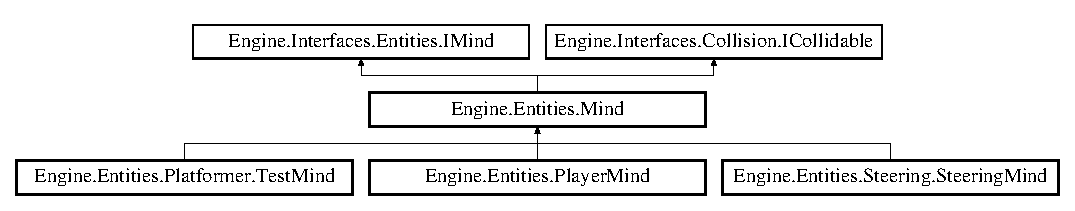
\includegraphics[height=2.393162cm]{d2/d41/a00318}
\end{center}
\end{figure}
\subsection*{Public Member Functions}
\begin{DoxyCompactItemize}
\item 
\hyperlink{a00318_aa352dcc92860d1304d4b1c71a0fe5d96}{Mind} ()
\begin{DoxyCompactList}\small\item\em C\+O\+N\+S\+T\+R\+U\+C\+T\+OR\+: \end{DoxyCompactList}\item 
\hyperlink{a00438}{I\+Entity} \hyperlink{a00318_a9585d4438e12299a42aaed4ee6fb88b6}{get\+Entity} ()
\begin{DoxyCompactList}\small\item\em M\+E\+T\+H\+OD\+: Get the entity which a mind controls. \end{DoxyCompactList}\item 
\hyperlink{a00426}{I\+Collidable} \hyperlink{a00318_aa36d6fcb8d80f1398855cea671ce1078}{get\+Collidable} ()
\begin{DoxyCompactList}\small\item\em M\+E\+T\+H\+OD\+: Return an object that will be calculated for collision \end{DoxyCompactList}\item 
virtual void \hyperlink{a00318_a386406a6250e4f7e59d0a048545ecc46}{Initialize} (Vector2 \hyperlink{a00318_ad94b3975c0873fee06b5bd5a75bd38cd}{Position}, string t)
\begin{DoxyCompactList}\small\item\em M\+E\+T\+H\+OD\+: Initialise the basic properties of the \hyperlink{a00318}{Mind} \end{DoxyCompactList}\item 
virtual void \hyperlink{a00318_a353d7d2bb1035aefebf0ae3e3f1d1488}{Initialize} (Vector2 \hyperlink{a00318_ad94b3975c0873fee06b5bd5a75bd38cd}{Position})
\begin{DoxyCompactList}\small\item\em M\+E\+T\+H\+OD\+: Initialises the basic properties of the mind when a texture has already been set \end{DoxyCompactList}\item 
virtual void \hyperlink{a00318_ac278d4358d794426251d1b87b6aa7b82}{On\+S\+A\+T\+Collision} (object sender, \hyperlink{a00350}{Collision\+Event\+Args} \hyperlink{a00318_ad89c9691d6b32053fe8ffcdeb68bdacf}{e})
\begin{DoxyCompactList}\small\item\em E\+V\+E\+NT\+: When S\+AT Collision returns true. \end{DoxyCompactList}\item 
virtual void \hyperlink{a00318_a15bf25a4a74706ef37592689f43c0598}{Unload} ()
\begin{DoxyCompactList}\small\item\em M\+E\+T\+H\+OD\+: Responsible for unloading anything added to this mind and sending it to the garbage collector \end{DoxyCompactList}\item 
void \hyperlink{a00318_a08db67e6cb8d5ff8015afa4fb780c5e8}{set\+Texture} (string t)
\begin{DoxyCompactList}\small\item\em M\+E\+T\+H\+OD\+: Set the texture of the entity this mind controls \end{DoxyCompactList}\item 
virtual void \hyperlink{a00318_adec6999d87accf7371de1536eac2541b}{Update} (Game\+Time game\+Time)
\begin{DoxyCompactList}\small\item\em M\+E\+T\+H\+OD\+: Update is called every frame and controls the main behaviour of the \hyperlink{a00318}{Mind}. \end{DoxyCompactList}\item 
void \hyperlink{a00318_a3f2db3b7d2b8b68a02b56472467ffd12}{Link} (\hyperlink{a00438}{I\+Entity} \hyperlink{a00318_ad89c9691d6b32053fe8ffcdeb68bdacf}{e})
\begin{DoxyCompactList}\small\item\em M\+E\+T\+H\+OD\+: Link the mind to an entity \end{DoxyCompactList}\item 
void \hyperlink{a00318_a4a05ceb8a5b1eb7f04e3111dd165b4b5}{Apply\+Force} (Vector2 force)
\item 
void \hyperlink{a00318_afc6609503e3a531416f5080b2114e24a}{Update\+Physics} ()
\begin{DoxyCompactList}\small\item\em M\+E\+T\+H\+OD\+: Simulates movement obeying the laws of physics \end{DoxyCompactList}\item 
void \hyperlink{a00318_a378218df0a8c27a981e98167197d9c16}{Apply\+Impulse} (Vector2 c\+Velocity)
\begin{DoxyCompactList}\small\item\em M\+E\+T\+H\+OD\+: Apply an impulse to an object once it has collided in order to simulate physics \end{DoxyCompactList}\end{DoxyCompactItemize}
\subsection*{Protected Attributes}
\begin{DoxyCompactItemize}
\item 
\hyperlink{a00438}{I\+Entity} \hyperlink{a00318_ad89c9691d6b32053fe8ffcdeb68bdacf}{e}
\begin{DoxyCompactList}\small\item\em D\+E\+C\+L\+A\+RE\+: The entity this mind will control. \end{DoxyCompactList}\item 
Vector2 \hyperlink{a00318_af56c17f56ba8133e32671318a6cc2c84}{velocity}
\begin{DoxyCompactList}\small\item\em G\+ET\+: S\+ET\+: The velocity of the mind \end{DoxyCompactList}\item 
Vector2 \hyperlink{a00318_a97534caf477680d0dcbe7021cc2b5a92}{acceleration} = new Vector2(0, 0)
\begin{DoxyCompactList}\small\item\em G\+ET\+: S\+ET\+: The acceleration of the mind \end{DoxyCompactList}\item 
float \hyperlink{a00318_a42f275657bd506946d9d7ec518cd4a22}{i\+Mass}
\begin{DoxyCompactList}\small\item\em G\+ET\+: S\+ET\+: The inverted Mass of the mind \end{DoxyCompactList}\item 
float \hyperlink{a00318_aca8c0c2865fe81c9bdabebcf7689c391}{restitution}
\begin{DoxyCompactList}\small\item\em G\+ET\+: S\+ET\+: The restitution of the mind \end{DoxyCompactList}\item 
float \hyperlink{a00318_aff4d26cdb8cbfeb96adfce9d92ddf5a0}{damping}
\begin{DoxyCompactList}\small\item\em G\+ET\+: S\+ET\+: the damping acting on the mind \end{DoxyCompactList}\item 
List$<$ \hyperlink{a00434}{I\+Hitbox} $>$ \hyperlink{a00318_a814329a8392c9a1f2d440c599dee3f91}{hits} = new List$<$\hyperlink{a00434}{I\+Hitbox}$>$()
\begin{DoxyCompactList}\small\item\em G\+ET\+: S\+ET\+: The list of hitboxes \end{DoxyCompactList}\item 
Vector2 \hyperlink{a00318_a5804486ad9da9f6220f390e94eb08ab7}{\+\_\+pos} = new Vector2()
\begin{DoxyCompactList}\small\item\em G\+ET\+: S\+ET\+: The position of the mind \end{DoxyCompactList}\item 
string \hyperlink{a00318_a0a20643f397ebed81d1b09965e0b6e3c}{tex\+Path} = \char`\"{}\char`\"{}
\begin{DoxyCompactList}\small\item\em D\+E\+C\+L\+A\+RE\+: The Texture path \end{DoxyCompactList}\end{DoxyCompactItemize}
\subsection*{Properties}
\begin{DoxyCompactItemize}
\item 
int \hyperlink{a00318_ab109f6638be56427f557f69b11beb995}{Unique\+ID}\hspace{0.3cm}{\ttfamily  \mbox{[}get, set\mbox{]}}
\begin{DoxyCompactList}\small\item\em G\+ET\+: S\+ET\+: The unique ID for the mind \end{DoxyCompactList}\item 
bool \hyperlink{a00318_add1498255352d92a5c96223a4d3cd657}{Active}\hspace{0.3cm}{\ttfamily  \mbox{[}get, set\mbox{]}}
\begin{DoxyCompactList}\small\item\em G\+ET\+: S\+ET\+: Whether the mind is active and in use or not. \end{DoxyCompactList}\item 
Vector2 \hyperlink{a00318_a5e95a120aad31ed943ae34b70083af85}{Velocity}\hspace{0.3cm}{\ttfamily  \mbox{[}get, set\mbox{]}}
\item 
Vector2 \hyperlink{a00318_ae117e7b4888d0d83ff72a586e9950b1e}{Acceleration}\hspace{0.3cm}{\ttfamily  \mbox{[}get, set\mbox{]}}
\item 
float \hyperlink{a00318_a7369f95c6d11a97fcf38873430b9d9a6}{Mass}\hspace{0.3cm}{\ttfamily  \mbox{[}get, set\mbox{]}}
\item 
float \hyperlink{a00318_a5d7175d3d87a533671551699c8bb93d0}{Restitution}\hspace{0.3cm}{\ttfamily  \mbox{[}get, set\mbox{]}}
\item 
float \hyperlink{a00318_a9e29defb461be7a43ce274f721fb1225}{Damping}\hspace{0.3cm}{\ttfamily  \mbox{[}get, set\mbox{]}}
\item 
List$<$ \hyperlink{a00434}{I\+Hitbox} $>$ \hyperlink{a00318_a09090a0316ecac49619a01a56a9a30b1}{Hits}\hspace{0.3cm}{\ttfamily  \mbox{[}get, set\mbox{]}}
\item 
bool \hyperlink{a00318_ab39c2af5a8338a67744d42891a2dc3ce}{is\+Colliding}\hspace{0.3cm}{\ttfamily  \mbox{[}get, set\mbox{]}}
\begin{DoxyCompactList}\small\item\em G\+ET\+: S\+ET\+: a bool to tell whether the mind is currently colliding \end{DoxyCompactList}\item 
Vector2 \hyperlink{a00318_ad94b3975c0873fee06b5bd5a75bd38cd}{Position}\hspace{0.3cm}{\ttfamily  \mbox{[}get, set\mbox{]}}
\item 
Rectangle \hyperlink{a00318_aa5a4c4b1e6b8373a14ee5e1a57a8ad54}{Bounds}\hspace{0.3cm}{\ttfamily  \mbox{[}get\mbox{]}}
\begin{DoxyCompactList}\small\item\em G\+ET\+: S\+ET\+: The Axis aligned bounds for the mind and entity \end{DoxyCompactList}\item 
bool \hyperlink{a00318_a4bf63dff33c53406b5342eb45e9627c4}{is\+Collidable}\hspace{0.3cm}{\ttfamily  \mbox{[}get, set\mbox{]}}
\begin{DoxyCompactList}\small\item\em G\+ET\+: S\+ET\+: Whether the object should be included in collision calculations \end{DoxyCompactList}\end{DoxyCompactItemize}


\subsection{Detailed Description}
A\+B\+S\+T\+R\+A\+CT C\+L\+A\+SS\+: \hyperlink{a00318}{Mind} controls the behaviour for a specific entity. The entity is simply the sprite that is drawn whilst \hyperlink{a00318}{Mind} controls how it acts. 



\subsection{Constructor \& Destructor Documentation}
\mbox{\Hypertarget{a00318_aa352dcc92860d1304d4b1c71a0fe5d96}\label{a00318_aa352dcc92860d1304d4b1c71a0fe5d96}} 
\index{Engine\+::\+Entities\+::\+Mind@{Engine\+::\+Entities\+::\+Mind}!Mind@{Mind}}
\index{Mind@{Mind}!Engine\+::\+Entities\+::\+Mind@{Engine\+::\+Entities\+::\+Mind}}
\subsubsection{\texorpdfstring{Mind()}{Mind()}}
{\footnotesize\ttfamily Engine.\+Entities.\+Mind.\+Mind (\begin{DoxyParamCaption}{ }\end{DoxyParamCaption})\hspace{0.3cm}{\ttfamily [inline]}}



C\+O\+N\+S\+T\+R\+U\+C\+T\+OR\+: 



\subsection{Member Function Documentation}
\mbox{\Hypertarget{a00318_a4a05ceb8a5b1eb7f04e3111dd165b4b5}\label{a00318_a4a05ceb8a5b1eb7f04e3111dd165b4b5}} 
\index{Engine\+::\+Entities\+::\+Mind@{Engine\+::\+Entities\+::\+Mind}!Apply\+Force@{Apply\+Force}}
\index{Apply\+Force@{Apply\+Force}!Engine\+::\+Entities\+::\+Mind@{Engine\+::\+Entities\+::\+Mind}}
\subsubsection{\texorpdfstring{Apply\+Force()}{ApplyForce()}}
{\footnotesize\ttfamily void Engine.\+Entities.\+Mind.\+Apply\+Force (\begin{DoxyParamCaption}\item[{Vector2}]{force }\end{DoxyParamCaption})\hspace{0.3cm}{\ttfamily [inline]}}

F = ma Therefore a = F/m but we are using inverse mass because multiplication is quicker than division, thus m is set to be equal to 1/m so we can do a = F $\ast$ m \mbox{\Hypertarget{a00318_a378218df0a8c27a981e98167197d9c16}\label{a00318_a378218df0a8c27a981e98167197d9c16}} 
\index{Engine\+::\+Entities\+::\+Mind@{Engine\+::\+Entities\+::\+Mind}!Apply\+Impulse@{Apply\+Impulse}}
\index{Apply\+Impulse@{Apply\+Impulse}!Engine\+::\+Entities\+::\+Mind@{Engine\+::\+Entities\+::\+Mind}}
\subsubsection{\texorpdfstring{Apply\+Impulse()}{ApplyImpulse()}}
{\footnotesize\ttfamily void Engine.\+Entities.\+Mind.\+Apply\+Impulse (\begin{DoxyParamCaption}\item[{Vector2}]{c\+Velocity }\end{DoxyParamCaption})\hspace{0.3cm}{\ttfamily [inline]}}



M\+E\+T\+H\+OD\+: Apply an impulse to an object once it has collided in order to simulate physics 


\begin{DoxyParams}{Parameters}
{\em c\+Velocity} & \\
\hline
\end{DoxyParams}
M\+U\+L\+T\+I\+P\+LY\+: The parameter closing velocity by the restitution

C\+A\+LL\+: Apply force with the closing velocity 

Implements \hyperlink{a00426_a000ca0336b06e3f2d658d442a83dbbbb}{Engine.\+Interfaces.\+Collision.\+I\+Collidable}.

\mbox{\Hypertarget{a00318_aa36d6fcb8d80f1398855cea671ce1078}\label{a00318_aa36d6fcb8d80f1398855cea671ce1078}} 
\index{Engine\+::\+Entities\+::\+Mind@{Engine\+::\+Entities\+::\+Mind}!get\+Collidable@{get\+Collidable}}
\index{get\+Collidable@{get\+Collidable}!Engine\+::\+Entities\+::\+Mind@{Engine\+::\+Entities\+::\+Mind}}
\subsubsection{\texorpdfstring{get\+Collidable()}{getCollidable()}}
{\footnotesize\ttfamily \hyperlink{a00426}{I\+Collidable} Engine.\+Entities.\+Mind.\+get\+Collidable (\begin{DoxyParamCaption}{ }\end{DoxyParamCaption})\hspace{0.3cm}{\ttfamily [inline]}}



M\+E\+T\+H\+OD\+: Return an object that will be calculated for collision 

\begin{DoxyReturn}{Returns}
An I\+Collidable of the current object
\end{DoxyReturn}


Implements \hyperlink{a00446_a3cbff0e85b710a4c8737254ed9ca7b30}{Engine.\+Interfaces.\+Entities.\+I\+Mind}.

\mbox{\Hypertarget{a00318_a9585d4438e12299a42aaed4ee6fb88b6}\label{a00318_a9585d4438e12299a42aaed4ee6fb88b6}} 
\index{Engine\+::\+Entities\+::\+Mind@{Engine\+::\+Entities\+::\+Mind}!get\+Entity@{get\+Entity}}
\index{get\+Entity@{get\+Entity}!Engine\+::\+Entities\+::\+Mind@{Engine\+::\+Entities\+::\+Mind}}
\subsubsection{\texorpdfstring{get\+Entity()}{getEntity()}}
{\footnotesize\ttfamily \hyperlink{a00438}{I\+Entity} Engine.\+Entities.\+Mind.\+get\+Entity (\begin{DoxyParamCaption}{ }\end{DoxyParamCaption})\hspace{0.3cm}{\ttfamily [inline]}}



M\+E\+T\+H\+OD\+: Get the entity which a mind controls. 

\begin{DoxyReturn}{Returns}
The I\+E\+Ntity this mind controls
\end{DoxyReturn}


Implements \hyperlink{a00446_af7c7cac5148930a12a85ec64412ac6f2}{Engine.\+Interfaces.\+Entities.\+I\+Mind}.

\mbox{\Hypertarget{a00318_a386406a6250e4f7e59d0a048545ecc46}\label{a00318_a386406a6250e4f7e59d0a048545ecc46}} 
\index{Engine\+::\+Entities\+::\+Mind@{Engine\+::\+Entities\+::\+Mind}!Initialize@{Initialize}}
\index{Initialize@{Initialize}!Engine\+::\+Entities\+::\+Mind@{Engine\+::\+Entities\+::\+Mind}}
\subsubsection{\texorpdfstring{Initialize()}{Initialize()}\hspace{0.1cm}{\footnotesize\ttfamily [1/2]}}
{\footnotesize\ttfamily virtual void Engine.\+Entities.\+Mind.\+Initialize (\begin{DoxyParamCaption}\item[{Vector2}]{Position,  }\item[{string}]{t }\end{DoxyParamCaption})\hspace{0.3cm}{\ttfamily [inline]}, {\ttfamily [virtual]}}



M\+E\+T\+H\+OD\+: Initialise the basic properties of the \hyperlink{a00318}{Mind} 


\begin{DoxyParams}{Parameters}
{\em Position} & \\
\hline
{\em t} & \\
\hline
\end{DoxyParams}
S\+ET\+: T\+He unique ID

C\+A\+LL\+: Set texture to set the texture

S\+ET\+: The position of the entity and whether the entity is visible

S\+ET\+: This mind to active 

Implements \hyperlink{a00446_a6f51a819769ba43f5f1702563293aacd}{Engine.\+Interfaces.\+Entities.\+I\+Mind}.

\mbox{\Hypertarget{a00318_a353d7d2bb1035aefebf0ae3e3f1d1488}\label{a00318_a353d7d2bb1035aefebf0ae3e3f1d1488}} 
\index{Engine\+::\+Entities\+::\+Mind@{Engine\+::\+Entities\+::\+Mind}!Initialize@{Initialize}}
\index{Initialize@{Initialize}!Engine\+::\+Entities\+::\+Mind@{Engine\+::\+Entities\+::\+Mind}}
\subsubsection{\texorpdfstring{Initialize()}{Initialize()}\hspace{0.1cm}{\footnotesize\ttfamily [2/2]}}
{\footnotesize\ttfamily virtual void Engine.\+Entities.\+Mind.\+Initialize (\begin{DoxyParamCaption}\item[{Vector2}]{Position }\end{DoxyParamCaption})\hspace{0.3cm}{\ttfamily [inline]}, {\ttfamily [virtual]}}



M\+E\+T\+H\+OD\+: Initialises the basic properties of the mind when a texture has already been set 


\begin{DoxyParams}{Parameters}
{\em Position} & \\
\hline
\end{DoxyParams}
H\+A\+N\+D\+L\+ER\+: Add handler for S\+AT collision

S\+ET\+: T\+He unique ID for this mind

IF\+: Texture path is not null

C\+A\+LL\+: Set texture

S\+ET\+: position and visibility of \hyperlink{a00314}{Entity} controlled by this mind.

S\+ET\+: The position of this mind and whether it is active. 

Implements \hyperlink{a00446_a421d8eb0a0accda3320144fbfe33ea8c}{Engine.\+Interfaces.\+Entities.\+I\+Mind}.



Reimplemented in \hyperlink{a00346_a72922ee865087d504b1bca3fec35fb6e}{Engine.\+Entities.\+Steering.\+Steering\+Mind}, \hyperlink{a00326_a44a3007533c5d73810c4636fcfef5988}{Engine.\+Entities.\+Player\+Mind}, and \hyperlink{a00334_ae94a647a0b9c6f1d99abb61e36612ba7}{Engine.\+Entities.\+Platformer.\+Test\+Mind}.

\mbox{\Hypertarget{a00318_a3f2db3b7d2b8b68a02b56472467ffd12}\label{a00318_a3f2db3b7d2b8b68a02b56472467ffd12}} 
\index{Engine\+::\+Entities\+::\+Mind@{Engine\+::\+Entities\+::\+Mind}!Link@{Link}}
\index{Link@{Link}!Engine\+::\+Entities\+::\+Mind@{Engine\+::\+Entities\+::\+Mind}}
\subsubsection{\texorpdfstring{Link()}{Link()}}
{\footnotesize\ttfamily void Engine.\+Entities.\+Mind.\+Link (\begin{DoxyParamCaption}\item[{\hyperlink{a00438}{I\+Entity}}]{e }\end{DoxyParamCaption})\hspace{0.3cm}{\ttfamily [inline]}}



M\+E\+T\+H\+OD\+: Link the mind to an entity 


\begin{DoxyParams}{Parameters}
{\em e} & \\
\hline
\end{DoxyParams}


Implements \hyperlink{a00446_a9d8370ad6e1b2a07760d3554b1e179fd}{Engine.\+Interfaces.\+Entities.\+I\+Mind}.

\mbox{\Hypertarget{a00318_ac278d4358d794426251d1b87b6aa7b82}\label{a00318_ac278d4358d794426251d1b87b6aa7b82}} 
\index{Engine\+::\+Entities\+::\+Mind@{Engine\+::\+Entities\+::\+Mind}!On\+S\+A\+T\+Collision@{On\+S\+A\+T\+Collision}}
\index{On\+S\+A\+T\+Collision@{On\+S\+A\+T\+Collision}!Engine\+::\+Entities\+::\+Mind@{Engine\+::\+Entities\+::\+Mind}}
\subsubsection{\texorpdfstring{On\+S\+A\+T\+Collision()}{OnSATCollision()}}
{\footnotesize\ttfamily virtual void Engine.\+Entities.\+Mind.\+On\+S\+A\+T\+Collision (\begin{DoxyParamCaption}\item[{object}]{sender,  }\item[{\hyperlink{a00350}{Collision\+Event\+Args}}]{e }\end{DoxyParamCaption})\hspace{0.3cm}{\ttfamily [inline]}, {\ttfamily [virtual]}}



E\+V\+E\+NT\+: When S\+AT Collision returns true. 


\begin{DoxyParams}{Parameters}
{\em sender} & \\
\hline
{\em e} & \\
\hline
\end{DoxyParams}
IF\+: This mind is object A, Apply Impulse to simulate physics

E\+L\+SE IF\+: this mind is object B, apply impulse in opposite direction 

Reimplemented in \hyperlink{a00346_a4834c17e78fd0bf82940ca0a4e8966f9}{Engine.\+Entities.\+Steering.\+Steering\+Mind}.

\mbox{\Hypertarget{a00318_a08db67e6cb8d5ff8015afa4fb780c5e8}\label{a00318_a08db67e6cb8d5ff8015afa4fb780c5e8}} 
\index{Engine\+::\+Entities\+::\+Mind@{Engine\+::\+Entities\+::\+Mind}!set\+Texture@{set\+Texture}}
\index{set\+Texture@{set\+Texture}!Engine\+::\+Entities\+::\+Mind@{Engine\+::\+Entities\+::\+Mind}}
\subsubsection{\texorpdfstring{set\+Texture()}{setTexture()}}
{\footnotesize\ttfamily void Engine.\+Entities.\+Mind.\+set\+Texture (\begin{DoxyParamCaption}\item[{string}]{t }\end{DoxyParamCaption})\hspace{0.3cm}{\ttfamily [inline]}}



M\+E\+T\+H\+OD\+: Set the texture of the entity this mind controls 


\begin{DoxyParams}{Parameters}
{\em t} & \\
\hline
\end{DoxyParams}
\mbox{\Hypertarget{a00318_a15bf25a4a74706ef37592689f43c0598}\label{a00318_a15bf25a4a74706ef37592689f43c0598}} 
\index{Engine\+::\+Entities\+::\+Mind@{Engine\+::\+Entities\+::\+Mind}!Unload@{Unload}}
\index{Unload@{Unload}!Engine\+::\+Entities\+::\+Mind@{Engine\+::\+Entities\+::\+Mind}}
\subsubsection{\texorpdfstring{Unload()}{Unload()}}
{\footnotesize\ttfamily virtual void Engine.\+Entities.\+Mind.\+Unload (\begin{DoxyParamCaption}{ }\end{DoxyParamCaption})\hspace{0.3cm}{\ttfamily [inline]}, {\ttfamily [virtual]}}



M\+E\+T\+H\+OD\+: Responsible for unloading anything added to this mind and sending it to the garbage collector 



Implements \hyperlink{a00446_a142493645e36a3e14c7d3c59793c4d3c}{Engine.\+Interfaces.\+Entities.\+I\+Mind}.



Reimplemented in \hyperlink{a00326_a80bacdc33e51129afed33f9e8bd5cd0f}{Engine.\+Entities.\+Player\+Mind}.

\mbox{\Hypertarget{a00318_adec6999d87accf7371de1536eac2541b}\label{a00318_adec6999d87accf7371de1536eac2541b}} 
\index{Engine\+::\+Entities\+::\+Mind@{Engine\+::\+Entities\+::\+Mind}!Update@{Update}}
\index{Update@{Update}!Engine\+::\+Entities\+::\+Mind@{Engine\+::\+Entities\+::\+Mind}}
\subsubsection{\texorpdfstring{Update()}{Update()}}
{\footnotesize\ttfamily virtual void Engine.\+Entities.\+Mind.\+Update (\begin{DoxyParamCaption}\item[{Game\+Time}]{game\+Time }\end{DoxyParamCaption})\hspace{0.3cm}{\ttfamily [inline]}, {\ttfamily [virtual]}}



M\+E\+T\+H\+OD\+: Update is called every frame and controls the main behaviour of the \hyperlink{a00318}{Mind}. 


\begin{DoxyParams}{Parameters}
{\em game\+Time} & \\
\hline
\end{DoxyParams}
S\+ET\+: Position of controlled entity

IF\+: \hyperlink{a00318}{Mind} is no longer active

S\+ET\+: entity to not be drawn

C\+A\+LL\+: Method to simulate physical movement 

Implements \hyperlink{a00446_a21a0486019d7c7b665fdf483626323f3}{Engine.\+Interfaces.\+Entities.\+I\+Mind}.



Reimplemented in \hyperlink{a00346_a2e1f7ec281cfe2b7e8268a93bec59d4a}{Engine.\+Entities.\+Steering.\+Steering\+Mind}, \hyperlink{a00326_a172dca0ea26dfd821b413f7592a98084}{Engine.\+Entities.\+Player\+Mind}, and \hyperlink{a00334_a1817f5df935d637c737d510e39fd251f}{Engine.\+Entities.\+Platformer.\+Test\+Mind}.

\mbox{\Hypertarget{a00318_afc6609503e3a531416f5080b2114e24a}\label{a00318_afc6609503e3a531416f5080b2114e24a}} 
\index{Engine\+::\+Entities\+::\+Mind@{Engine\+::\+Entities\+::\+Mind}!Update\+Physics@{Update\+Physics}}
\index{Update\+Physics@{Update\+Physics}!Engine\+::\+Entities\+::\+Mind@{Engine\+::\+Entities\+::\+Mind}}
\subsubsection{\texorpdfstring{Update\+Physics()}{UpdatePhysics()}}
{\footnotesize\ttfamily void Engine.\+Entities.\+Mind.\+Update\+Physics (\begin{DoxyParamCaption}{ }\end{DoxyParamCaption})\hspace{0.3cm}{\ttfamily [inline]}}



M\+E\+T\+H\+OD\+: Simulates movement obeying the laws of physics 

M\+U\+L\+T\+I\+P\+LY\+: the velocity by the damping force

A\+DD\+: The acceleration onto the velocity

A\+DD\+: The velocity onto the position

F\+OR\+: Each hitbox this mind controls

S\+ET\+: the velocity of the hitbox to this velocity

F\+OR\+: Each hitbox this mind controls

S\+ET\+: the points on each hitbox relative to the entity

S\+ET\+: acceleration to 0 

\subsection{Field Documentation}
\mbox{\Hypertarget{a00318_a5804486ad9da9f6220f390e94eb08ab7}\label{a00318_a5804486ad9da9f6220f390e94eb08ab7}} 
\index{Engine\+::\+Entities\+::\+Mind@{Engine\+::\+Entities\+::\+Mind}!\+\_\+pos@{\+\_\+pos}}
\index{\+\_\+pos@{\+\_\+pos}!Engine\+::\+Entities\+::\+Mind@{Engine\+::\+Entities\+::\+Mind}}
\subsubsection{\texorpdfstring{\+\_\+pos}{\_pos}}
{\footnotesize\ttfamily Vector2 Engine.\+Entities.\+Mind.\+\_\+pos = new Vector2()\hspace{0.3cm}{\ttfamily [protected]}}



G\+ET\+: S\+ET\+: The position of the mind 

\mbox{\Hypertarget{a00318_a97534caf477680d0dcbe7021cc2b5a92}\label{a00318_a97534caf477680d0dcbe7021cc2b5a92}} 
\index{Engine\+::\+Entities\+::\+Mind@{Engine\+::\+Entities\+::\+Mind}!acceleration@{acceleration}}
\index{acceleration@{acceleration}!Engine\+::\+Entities\+::\+Mind@{Engine\+::\+Entities\+::\+Mind}}
\subsubsection{\texorpdfstring{acceleration}{acceleration}}
{\footnotesize\ttfamily Vector2 Engine.\+Entities.\+Mind.\+acceleration = new Vector2(0, 0)\hspace{0.3cm}{\ttfamily [protected]}}



G\+ET\+: S\+ET\+: The acceleration of the mind 

\mbox{\Hypertarget{a00318_aff4d26cdb8cbfeb96adfce9d92ddf5a0}\label{a00318_aff4d26cdb8cbfeb96adfce9d92ddf5a0}} 
\index{Engine\+::\+Entities\+::\+Mind@{Engine\+::\+Entities\+::\+Mind}!damping@{damping}}
\index{damping@{damping}!Engine\+::\+Entities\+::\+Mind@{Engine\+::\+Entities\+::\+Mind}}
\subsubsection{\texorpdfstring{damping}{damping}}
{\footnotesize\ttfamily float Engine.\+Entities.\+Mind.\+damping\hspace{0.3cm}{\ttfamily [protected]}}



G\+ET\+: S\+ET\+: the damping acting on the mind 

\mbox{\Hypertarget{a00318_ad89c9691d6b32053fe8ffcdeb68bdacf}\label{a00318_ad89c9691d6b32053fe8ffcdeb68bdacf}} 
\index{Engine\+::\+Entities\+::\+Mind@{Engine\+::\+Entities\+::\+Mind}!e@{e}}
\index{e@{e}!Engine\+::\+Entities\+::\+Mind@{Engine\+::\+Entities\+::\+Mind}}
\subsubsection{\texorpdfstring{e}{e}}
{\footnotesize\ttfamily \hyperlink{a00438}{I\+Entity} Engine.\+Entities.\+Mind.\+e\hspace{0.3cm}{\ttfamily [protected]}}



D\+E\+C\+L\+A\+RE\+: The entity this mind will control. 

\mbox{\Hypertarget{a00318_a814329a8392c9a1f2d440c599dee3f91}\label{a00318_a814329a8392c9a1f2d440c599dee3f91}} 
\index{Engine\+::\+Entities\+::\+Mind@{Engine\+::\+Entities\+::\+Mind}!hits@{hits}}
\index{hits@{hits}!Engine\+::\+Entities\+::\+Mind@{Engine\+::\+Entities\+::\+Mind}}
\subsubsection{\texorpdfstring{hits}{hits}}
{\footnotesize\ttfamily List$<$\hyperlink{a00434}{I\+Hitbox}$>$ Engine.\+Entities.\+Mind.\+hits = new List$<$\hyperlink{a00434}{I\+Hitbox}$>$()\hspace{0.3cm}{\ttfamily [protected]}}



G\+ET\+: S\+ET\+: The list of hitboxes 

\mbox{\Hypertarget{a00318_a42f275657bd506946d9d7ec518cd4a22}\label{a00318_a42f275657bd506946d9d7ec518cd4a22}} 
\index{Engine\+::\+Entities\+::\+Mind@{Engine\+::\+Entities\+::\+Mind}!i\+Mass@{i\+Mass}}
\index{i\+Mass@{i\+Mass}!Engine\+::\+Entities\+::\+Mind@{Engine\+::\+Entities\+::\+Mind}}
\subsubsection{\texorpdfstring{i\+Mass}{iMass}}
{\footnotesize\ttfamily float Engine.\+Entities.\+Mind.\+i\+Mass\hspace{0.3cm}{\ttfamily [protected]}}



G\+ET\+: S\+ET\+: The inverted Mass of the mind 

\mbox{\Hypertarget{a00318_aca8c0c2865fe81c9bdabebcf7689c391}\label{a00318_aca8c0c2865fe81c9bdabebcf7689c391}} 
\index{Engine\+::\+Entities\+::\+Mind@{Engine\+::\+Entities\+::\+Mind}!restitution@{restitution}}
\index{restitution@{restitution}!Engine\+::\+Entities\+::\+Mind@{Engine\+::\+Entities\+::\+Mind}}
\subsubsection{\texorpdfstring{restitution}{restitution}}
{\footnotesize\ttfamily float Engine.\+Entities.\+Mind.\+restitution\hspace{0.3cm}{\ttfamily [protected]}}



G\+ET\+: S\+ET\+: The restitution of the mind 

\mbox{\Hypertarget{a00318_a0a20643f397ebed81d1b09965e0b6e3c}\label{a00318_a0a20643f397ebed81d1b09965e0b6e3c}} 
\index{Engine\+::\+Entities\+::\+Mind@{Engine\+::\+Entities\+::\+Mind}!tex\+Path@{tex\+Path}}
\index{tex\+Path@{tex\+Path}!Engine\+::\+Entities\+::\+Mind@{Engine\+::\+Entities\+::\+Mind}}
\subsubsection{\texorpdfstring{tex\+Path}{texPath}}
{\footnotesize\ttfamily string Engine.\+Entities.\+Mind.\+tex\+Path = \char`\"{}\char`\"{}\hspace{0.3cm}{\ttfamily [protected]}}



D\+E\+C\+L\+A\+RE\+: The Texture path 

\mbox{\Hypertarget{a00318_af56c17f56ba8133e32671318a6cc2c84}\label{a00318_af56c17f56ba8133e32671318a6cc2c84}} 
\index{Engine\+::\+Entities\+::\+Mind@{Engine\+::\+Entities\+::\+Mind}!velocity@{velocity}}
\index{velocity@{velocity}!Engine\+::\+Entities\+::\+Mind@{Engine\+::\+Entities\+::\+Mind}}
\subsubsection{\texorpdfstring{velocity}{velocity}}
{\footnotesize\ttfamily Vector2 Engine.\+Entities.\+Mind.\+velocity\hspace{0.3cm}{\ttfamily [protected]}}



G\+ET\+: S\+ET\+: The velocity of the mind 



\subsection{Property Documentation}
\mbox{\Hypertarget{a00318_ae117e7b4888d0d83ff72a586e9950b1e}\label{a00318_ae117e7b4888d0d83ff72a586e9950b1e}} 
\index{Engine\+::\+Entities\+::\+Mind@{Engine\+::\+Entities\+::\+Mind}!Acceleration@{Acceleration}}
\index{Acceleration@{Acceleration}!Engine\+::\+Entities\+::\+Mind@{Engine\+::\+Entities\+::\+Mind}}
\subsubsection{\texorpdfstring{Acceleration}{Acceleration}}
{\footnotesize\ttfamily Vector2 Engine.\+Entities.\+Mind.\+Acceleration\hspace{0.3cm}{\ttfamily [get]}, {\ttfamily [set]}}

\mbox{\Hypertarget{a00318_add1498255352d92a5c96223a4d3cd657}\label{a00318_add1498255352d92a5c96223a4d3cd657}} 
\index{Engine\+::\+Entities\+::\+Mind@{Engine\+::\+Entities\+::\+Mind}!Active@{Active}}
\index{Active@{Active}!Engine\+::\+Entities\+::\+Mind@{Engine\+::\+Entities\+::\+Mind}}
\subsubsection{\texorpdfstring{Active}{Active}}
{\footnotesize\ttfamily bool Engine.\+Entities.\+Mind.\+Active\hspace{0.3cm}{\ttfamily [get]}, {\ttfamily [set]}}



G\+ET\+: S\+ET\+: Whether the mind is active and in use or not. 

\mbox{\Hypertarget{a00318_aa5a4c4b1e6b8373a14ee5e1a57a8ad54}\label{a00318_aa5a4c4b1e6b8373a14ee5e1a57a8ad54}} 
\index{Engine\+::\+Entities\+::\+Mind@{Engine\+::\+Entities\+::\+Mind}!Bounds@{Bounds}}
\index{Bounds@{Bounds}!Engine\+::\+Entities\+::\+Mind@{Engine\+::\+Entities\+::\+Mind}}
\subsubsection{\texorpdfstring{Bounds}{Bounds}}
{\footnotesize\ttfamily Rectangle Engine.\+Entities.\+Mind.\+Bounds\hspace{0.3cm}{\ttfamily [get]}}



G\+ET\+: S\+ET\+: The Axis aligned bounds for the mind and entity 

\mbox{\Hypertarget{a00318_a9e29defb461be7a43ce274f721fb1225}\label{a00318_a9e29defb461be7a43ce274f721fb1225}} 
\index{Engine\+::\+Entities\+::\+Mind@{Engine\+::\+Entities\+::\+Mind}!Damping@{Damping}}
\index{Damping@{Damping}!Engine\+::\+Entities\+::\+Mind@{Engine\+::\+Entities\+::\+Mind}}
\subsubsection{\texorpdfstring{Damping}{Damping}}
{\footnotesize\ttfamily float Engine.\+Entities.\+Mind.\+Damping\hspace{0.3cm}{\ttfamily [get]}, {\ttfamily [set]}}

\mbox{\Hypertarget{a00318_a09090a0316ecac49619a01a56a9a30b1}\label{a00318_a09090a0316ecac49619a01a56a9a30b1}} 
\index{Engine\+::\+Entities\+::\+Mind@{Engine\+::\+Entities\+::\+Mind}!Hits@{Hits}}
\index{Hits@{Hits}!Engine\+::\+Entities\+::\+Mind@{Engine\+::\+Entities\+::\+Mind}}
\subsubsection{\texorpdfstring{Hits}{Hits}}
{\footnotesize\ttfamily List$<$\hyperlink{a00434}{I\+Hitbox}$>$ Engine.\+Entities.\+Mind.\+Hits\hspace{0.3cm}{\ttfamily [get]}, {\ttfamily [set]}}

\mbox{\Hypertarget{a00318_a4bf63dff33c53406b5342eb45e9627c4}\label{a00318_a4bf63dff33c53406b5342eb45e9627c4}} 
\index{Engine\+::\+Entities\+::\+Mind@{Engine\+::\+Entities\+::\+Mind}!is\+Collidable@{is\+Collidable}}
\index{is\+Collidable@{is\+Collidable}!Engine\+::\+Entities\+::\+Mind@{Engine\+::\+Entities\+::\+Mind}}
\subsubsection{\texorpdfstring{is\+Collidable}{isCollidable}}
{\footnotesize\ttfamily bool Engine.\+Entities.\+Mind.\+is\+Collidable\hspace{0.3cm}{\ttfamily [get]}, {\ttfamily [set]}}



G\+ET\+: S\+ET\+: Whether the object should be included in collision calculations 

\mbox{\Hypertarget{a00318_ab39c2af5a8338a67744d42891a2dc3ce}\label{a00318_ab39c2af5a8338a67744d42891a2dc3ce}} 
\index{Engine\+::\+Entities\+::\+Mind@{Engine\+::\+Entities\+::\+Mind}!is\+Colliding@{is\+Colliding}}
\index{is\+Colliding@{is\+Colliding}!Engine\+::\+Entities\+::\+Mind@{Engine\+::\+Entities\+::\+Mind}}
\subsubsection{\texorpdfstring{is\+Colliding}{isColliding}}
{\footnotesize\ttfamily bool Engine.\+Entities.\+Mind.\+is\+Colliding\hspace{0.3cm}{\ttfamily [get]}, {\ttfamily [set]}}



G\+ET\+: S\+ET\+: a bool to tell whether the mind is currently colliding 

\mbox{\Hypertarget{a00318_a7369f95c6d11a97fcf38873430b9d9a6}\label{a00318_a7369f95c6d11a97fcf38873430b9d9a6}} 
\index{Engine\+::\+Entities\+::\+Mind@{Engine\+::\+Entities\+::\+Mind}!Mass@{Mass}}
\index{Mass@{Mass}!Engine\+::\+Entities\+::\+Mind@{Engine\+::\+Entities\+::\+Mind}}
\subsubsection{\texorpdfstring{Mass}{Mass}}
{\footnotesize\ttfamily float Engine.\+Entities.\+Mind.\+Mass\hspace{0.3cm}{\ttfamily [get]}, {\ttfamily [set]}}

\mbox{\Hypertarget{a00318_ad94b3975c0873fee06b5bd5a75bd38cd}\label{a00318_ad94b3975c0873fee06b5bd5a75bd38cd}} 
\index{Engine\+::\+Entities\+::\+Mind@{Engine\+::\+Entities\+::\+Mind}!Position@{Position}}
\index{Position@{Position}!Engine\+::\+Entities\+::\+Mind@{Engine\+::\+Entities\+::\+Mind}}
\subsubsection{\texorpdfstring{Position}{Position}}
{\footnotesize\ttfamily Vector2 Engine.\+Entities.\+Mind.\+Position\hspace{0.3cm}{\ttfamily [get]}, {\ttfamily [set]}}

\mbox{\Hypertarget{a00318_a5d7175d3d87a533671551699c8bb93d0}\label{a00318_a5d7175d3d87a533671551699c8bb93d0}} 
\index{Engine\+::\+Entities\+::\+Mind@{Engine\+::\+Entities\+::\+Mind}!Restitution@{Restitution}}
\index{Restitution@{Restitution}!Engine\+::\+Entities\+::\+Mind@{Engine\+::\+Entities\+::\+Mind}}
\subsubsection{\texorpdfstring{Restitution}{Restitution}}
{\footnotesize\ttfamily float Engine.\+Entities.\+Mind.\+Restitution\hspace{0.3cm}{\ttfamily [get]}, {\ttfamily [set]}}

\mbox{\Hypertarget{a00318_ab109f6638be56427f557f69b11beb995}\label{a00318_ab109f6638be56427f557f69b11beb995}} 
\index{Engine\+::\+Entities\+::\+Mind@{Engine\+::\+Entities\+::\+Mind}!Unique\+ID@{Unique\+ID}}
\index{Unique\+ID@{Unique\+ID}!Engine\+::\+Entities\+::\+Mind@{Engine\+::\+Entities\+::\+Mind}}
\subsubsection{\texorpdfstring{Unique\+ID}{UniqueID}}
{\footnotesize\ttfamily int Engine.\+Entities.\+Mind.\+Unique\+ID\hspace{0.3cm}{\ttfamily [get]}, {\ttfamily [set]}}



G\+ET\+: S\+ET\+: The unique ID for the mind 

\mbox{\Hypertarget{a00318_a5e95a120aad31ed943ae34b70083af85}\label{a00318_a5e95a120aad31ed943ae34b70083af85}} 
\index{Engine\+::\+Entities\+::\+Mind@{Engine\+::\+Entities\+::\+Mind}!Velocity@{Velocity}}
\index{Velocity@{Velocity}!Engine\+::\+Entities\+::\+Mind@{Engine\+::\+Entities\+::\+Mind}}
\subsubsection{\texorpdfstring{Velocity}{Velocity}}
{\footnotesize\ttfamily Vector2 Engine.\+Entities.\+Mind.\+Velocity\hspace{0.3cm}{\ttfamily [get]}, {\ttfamily [set]}}



The documentation for this class was generated from the following file\+:\begin{DoxyCompactItemize}
\item 
\hyperlink{a00020}{Mind.\+cs}\end{DoxyCompactItemize}

\hypertarget{a00374}{}\section{Engine.\+Events.\+Mouse\+Event.\+Mouse\+Event\+Args Class Reference}
\label{a00374}\index{Engine.\+Events.\+Mouse\+Event.\+Mouse\+Event\+Args@{Engine.\+Events.\+Mouse\+Event.\+Mouse\+Event\+Args}}
Inheritance diagram for Engine.\+Events.\+Mouse\+Event.\+Mouse\+Event\+Args\+:\begin{figure}[H]
\begin{center}
\leavevmode
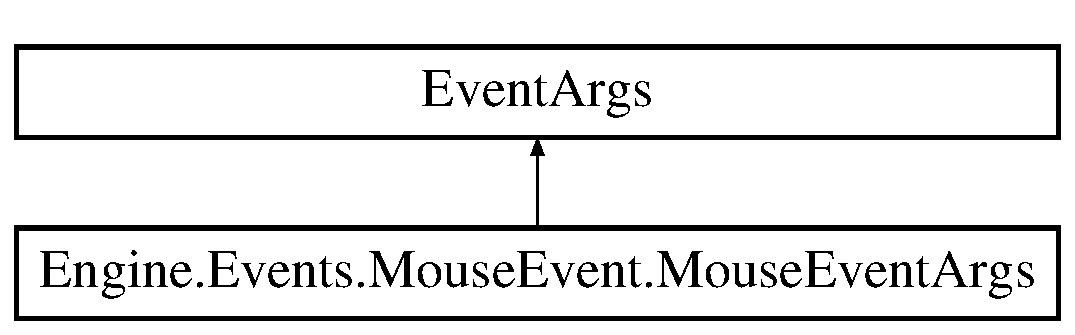
\includegraphics[height=2.000000cm]{d5/db5/a00374}
\end{center}
\end{figure}
\subsection*{Properties}
\begin{DoxyCompactItemize}
\item 
int \hyperlink{a00374_a175240a0014c598ad4d3daa2c1ab2a52}{X}\hspace{0.3cm}{\ttfamily  \mbox{[}get\mbox{]}}
\item 
int \hyperlink{a00374_aeb28044ee25cb17021a05179d2bdf2cf}{Y}\hspace{0.3cm}{\ttfamily  \mbox{[}get\mbox{]}}
\item 
Button\+State \hyperlink{a00374_ade52d4638272eb8342e036b3d0fd6dc7}{current\+Button}\hspace{0.3cm}{\ttfamily  \mbox{[}get, set\mbox{]}}
\item 
Mouse\+State \hyperlink{a00374_ae98190023f0a49b913faddf08e76b75a}{mouse\+State}\hspace{0.3cm}{\ttfamily  \mbox{[}get, set\mbox{]}}
\item 
Rectangle \hyperlink{a00374_a3f65de8a63ad6d5135dd71c181cb0fc4}{Bounds}\hspace{0.3cm}{\ttfamily  \mbox{[}get\mbox{]}}
\item 
Rectangle \hyperlink{a00374_abb545612ce32e2f770e0c199193a28a1}{bounds\+To\+World\+View}\hspace{0.3cm}{\ttfamily  \mbox{[}get\mbox{]}}
\end{DoxyCompactItemize}


\subsection{Property Documentation}
\mbox{\Hypertarget{a00374_a3f65de8a63ad6d5135dd71c181cb0fc4}\label{a00374_a3f65de8a63ad6d5135dd71c181cb0fc4}} 
\index{Engine\+::\+Events\+::\+Mouse\+Event\+::\+Mouse\+Event\+Args@{Engine\+::\+Events\+::\+Mouse\+Event\+::\+Mouse\+Event\+Args}!Bounds@{Bounds}}
\index{Bounds@{Bounds}!Engine\+::\+Events\+::\+Mouse\+Event\+::\+Mouse\+Event\+Args@{Engine\+::\+Events\+::\+Mouse\+Event\+::\+Mouse\+Event\+Args}}
\subsubsection{\texorpdfstring{Bounds}{Bounds}}
{\footnotesize\ttfamily Rectangle Engine.\+Events.\+Mouse\+Event.\+Mouse\+Event\+Args.\+Bounds\hspace{0.3cm}{\ttfamily [get]}}

\mbox{\Hypertarget{a00374_abb545612ce32e2f770e0c199193a28a1}\label{a00374_abb545612ce32e2f770e0c199193a28a1}} 
\index{Engine\+::\+Events\+::\+Mouse\+Event\+::\+Mouse\+Event\+Args@{Engine\+::\+Events\+::\+Mouse\+Event\+::\+Mouse\+Event\+Args}!bounds\+To\+World\+View@{bounds\+To\+World\+View}}
\index{bounds\+To\+World\+View@{bounds\+To\+World\+View}!Engine\+::\+Events\+::\+Mouse\+Event\+::\+Mouse\+Event\+Args@{Engine\+::\+Events\+::\+Mouse\+Event\+::\+Mouse\+Event\+Args}}
\subsubsection{\texorpdfstring{bounds\+To\+World\+View}{boundsToWorldView}}
{\footnotesize\ttfamily Rectangle Engine.\+Events.\+Mouse\+Event.\+Mouse\+Event\+Args.\+bounds\+To\+World\+View\hspace{0.3cm}{\ttfamily [get]}}

\mbox{\Hypertarget{a00374_ade52d4638272eb8342e036b3d0fd6dc7}\label{a00374_ade52d4638272eb8342e036b3d0fd6dc7}} 
\index{Engine\+::\+Events\+::\+Mouse\+Event\+::\+Mouse\+Event\+Args@{Engine\+::\+Events\+::\+Mouse\+Event\+::\+Mouse\+Event\+Args}!current\+Button@{current\+Button}}
\index{current\+Button@{current\+Button}!Engine\+::\+Events\+::\+Mouse\+Event\+::\+Mouse\+Event\+Args@{Engine\+::\+Events\+::\+Mouse\+Event\+::\+Mouse\+Event\+Args}}
\subsubsection{\texorpdfstring{current\+Button}{currentButton}}
{\footnotesize\ttfamily Button\+State Engine.\+Events.\+Mouse\+Event.\+Mouse\+Event\+Args.\+current\+Button\hspace{0.3cm}{\ttfamily [get]}, {\ttfamily [set]}}

\mbox{\Hypertarget{a00374_ae98190023f0a49b913faddf08e76b75a}\label{a00374_ae98190023f0a49b913faddf08e76b75a}} 
\index{Engine\+::\+Events\+::\+Mouse\+Event\+::\+Mouse\+Event\+Args@{Engine\+::\+Events\+::\+Mouse\+Event\+::\+Mouse\+Event\+Args}!mouse\+State@{mouse\+State}}
\index{mouse\+State@{mouse\+State}!Engine\+::\+Events\+::\+Mouse\+Event\+::\+Mouse\+Event\+Args@{Engine\+::\+Events\+::\+Mouse\+Event\+::\+Mouse\+Event\+Args}}
\subsubsection{\texorpdfstring{mouse\+State}{mouseState}}
{\footnotesize\ttfamily Mouse\+State Engine.\+Events.\+Mouse\+Event.\+Mouse\+Event\+Args.\+mouse\+State\hspace{0.3cm}{\ttfamily [get]}, {\ttfamily [set]}}

\mbox{\Hypertarget{a00374_a175240a0014c598ad4d3daa2c1ab2a52}\label{a00374_a175240a0014c598ad4d3daa2c1ab2a52}} 
\index{Engine\+::\+Events\+::\+Mouse\+Event\+::\+Mouse\+Event\+Args@{Engine\+::\+Events\+::\+Mouse\+Event\+::\+Mouse\+Event\+Args}!X@{X}}
\index{X@{X}!Engine\+::\+Events\+::\+Mouse\+Event\+::\+Mouse\+Event\+Args@{Engine\+::\+Events\+::\+Mouse\+Event\+::\+Mouse\+Event\+Args}}
\subsubsection{\texorpdfstring{X}{X}}
{\footnotesize\ttfamily int Engine.\+Events.\+Mouse\+Event.\+Mouse\+Event\+Args.\+X\hspace{0.3cm}{\ttfamily [get]}}

\mbox{\Hypertarget{a00374_aeb28044ee25cb17021a05179d2bdf2cf}\label{a00374_aeb28044ee25cb17021a05179d2bdf2cf}} 
\index{Engine\+::\+Events\+::\+Mouse\+Event\+::\+Mouse\+Event\+Args@{Engine\+::\+Events\+::\+Mouse\+Event\+::\+Mouse\+Event\+Args}!Y@{Y}}
\index{Y@{Y}!Engine\+::\+Events\+::\+Mouse\+Event\+::\+Mouse\+Event\+Args@{Engine\+::\+Events\+::\+Mouse\+Event\+::\+Mouse\+Event\+Args}}
\subsubsection{\texorpdfstring{Y}{Y}}
{\footnotesize\ttfamily int Engine.\+Events.\+Mouse\+Event.\+Mouse\+Event\+Args.\+Y\hspace{0.3cm}{\ttfamily [get]}}



The documentation for this class was generated from the following file\+:\begin{DoxyCompactItemize}
\item 
\hyperlink{a00062}{Mouse\+Event\+Args.\+cs}\end{DoxyCompactItemize}

\hypertarget{a00378}{}\section{Engine.\+Events.\+Mouse\+Event.\+Mouse\+Handler Class Reference}
\label{a00378}\index{Engine.\+Events.\+Mouse\+Event.\+Mouse\+Handler@{Engine.\+Events.\+Mouse\+Event.\+Mouse\+Handler}}
Inheritance diagram for Engine.\+Events.\+Mouse\+Event.\+Mouse\+Handler\+:\begin{figure}[H]
\begin{center}
\leavevmode
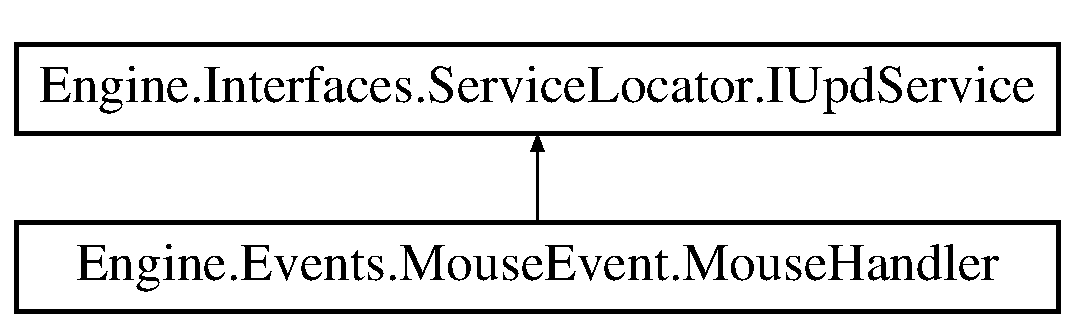
\includegraphics[height=2.000000cm]{d7/d08/a00378}
\end{center}
\end{figure}
\subsection*{Public Member Functions}
\begin{DoxyCompactItemize}
\item 
delegate void \hyperlink{a00378_a932e0a6ed83094bb6fa33a6ae64be38a}{Mouse\+Event\+Handler} (object sender, \hyperlink{a00374}{Mouse\+Event\+Args} e)
\item 
void \hyperlink{a00378_ad6c588c046d6a350498fd7875416a151}{Update} (Game\+Time game\+Time)
\begin{DoxyCompactList}\small\item\em M\+E\+T\+H\+OD\+: The update loop which is cycled through ever frame \end{DoxyCompactList}\end{DoxyCompactItemize}
\subsection*{Protected Member Functions}
\begin{DoxyCompactItemize}
\item 
virtual void \hyperlink{a00378_a6e2564dfdc8136f81013f97c594ab217}{On\+Mouse\+Down} (Mouse\+State m)
\item 
virtual void \hyperlink{a00378_af7d850a3b88a8367991f3ac957f1e482}{On\+Mouse\+Scroll\+Up} (Mouse\+State m)
\item 
virtual void \hyperlink{a00378_a20e5fe1f5e747900bdc0f389aae9b935}{On\+Mouse\+Scroll\+Down} (Mouse\+State m)
\item 
virtual void \hyperlink{a00378_a7337e5e2c83fe6946a93d6f1a57bcdd4}{On\+Mouse\+Released} (Mouse\+State m)
\item 
virtual void \hyperlink{a00378_a69716c4b0f065d5939ce73f39999e497}{On\+Mouse\+Moved} (Mouse\+State m)
\end{DoxyCompactItemize}
\subsection*{Events}
\begin{DoxyCompactItemize}
\item 
\hyperlink{a00378_a932e0a6ed83094bb6fa33a6ae64be38a}{Mouse\+Event\+Handler} \hyperlink{a00378_ae6859271609356f4c6e30fbdcdda28a9}{Mouse\+Click}
\item 
\hyperlink{a00378_a932e0a6ed83094bb6fa33a6ae64be38a}{Mouse\+Event\+Handler} \hyperlink{a00378_aa7e294c0752f892e917d7788818dd685}{Mouse\+Released}
\item 
\hyperlink{a00378_a932e0a6ed83094bb6fa33a6ae64be38a}{Mouse\+Event\+Handler} \hyperlink{a00378_a6d61cfd953bda3531ea16380df4d8e59}{Mouse\+Moved}
\item 
\hyperlink{a00378_a932e0a6ed83094bb6fa33a6ae64be38a}{Mouse\+Event\+Handler} \hyperlink{a00378_ac2b72a0951f5946b97d65479cacb5634}{Mouse\+Held}
\item 
\hyperlink{a00378_a932e0a6ed83094bb6fa33a6ae64be38a}{Mouse\+Event\+Handler} \hyperlink{a00378_aa534e523c05b4c0eb558a62e932c063a}{Mouse\+Scroll\+Up}
\item 
\hyperlink{a00378_a932e0a6ed83094bb6fa33a6ae64be38a}{Mouse\+Event\+Handler} \hyperlink{a00378_aba8754542d3586f246a92a726427bf73}{Mouse\+Scroll\+Down}
\end{DoxyCompactItemize}


\subsection{Member Function Documentation}
\mbox{\Hypertarget{a00378_a932e0a6ed83094bb6fa33a6ae64be38a}\label{a00378_a932e0a6ed83094bb6fa33a6ae64be38a}} 
\index{Engine\+::\+Events\+::\+Mouse\+Event\+::\+Mouse\+Handler@{Engine\+::\+Events\+::\+Mouse\+Event\+::\+Mouse\+Handler}!Mouse\+Event\+Handler@{Mouse\+Event\+Handler}}
\index{Mouse\+Event\+Handler@{Mouse\+Event\+Handler}!Engine\+::\+Events\+::\+Mouse\+Event\+::\+Mouse\+Handler@{Engine\+::\+Events\+::\+Mouse\+Event\+::\+Mouse\+Handler}}
\subsubsection{\texorpdfstring{Mouse\+Event\+Handler()}{MouseEventHandler()}}
{\footnotesize\ttfamily delegate void Engine.\+Events.\+Mouse\+Event.\+Mouse\+Handler.\+Mouse\+Event\+Handler (\begin{DoxyParamCaption}\item[{object}]{sender,  }\item[{\hyperlink{a00374}{Mouse\+Event\+Args}}]{e }\end{DoxyParamCaption})}

\mbox{\Hypertarget{a00378_a6e2564dfdc8136f81013f97c594ab217}\label{a00378_a6e2564dfdc8136f81013f97c594ab217}} 
\index{Engine\+::\+Events\+::\+Mouse\+Event\+::\+Mouse\+Handler@{Engine\+::\+Events\+::\+Mouse\+Event\+::\+Mouse\+Handler}!On\+Mouse\+Down@{On\+Mouse\+Down}}
\index{On\+Mouse\+Down@{On\+Mouse\+Down}!Engine\+::\+Events\+::\+Mouse\+Event\+::\+Mouse\+Handler@{Engine\+::\+Events\+::\+Mouse\+Event\+::\+Mouse\+Handler}}
\subsubsection{\texorpdfstring{On\+Mouse\+Down()}{OnMouseDown()}}
{\footnotesize\ttfamily virtual void Engine.\+Events.\+Mouse\+Event.\+Mouse\+Handler.\+On\+Mouse\+Down (\begin{DoxyParamCaption}\item[{Mouse\+State}]{m }\end{DoxyParamCaption})\hspace{0.3cm}{\ttfamily [inline]}, {\ttfamily [protected]}, {\ttfamily [virtual]}}

\mbox{\Hypertarget{a00378_a69716c4b0f065d5939ce73f39999e497}\label{a00378_a69716c4b0f065d5939ce73f39999e497}} 
\index{Engine\+::\+Events\+::\+Mouse\+Event\+::\+Mouse\+Handler@{Engine\+::\+Events\+::\+Mouse\+Event\+::\+Mouse\+Handler}!On\+Mouse\+Moved@{On\+Mouse\+Moved}}
\index{On\+Mouse\+Moved@{On\+Mouse\+Moved}!Engine\+::\+Events\+::\+Mouse\+Event\+::\+Mouse\+Handler@{Engine\+::\+Events\+::\+Mouse\+Event\+::\+Mouse\+Handler}}
\subsubsection{\texorpdfstring{On\+Mouse\+Moved()}{OnMouseMoved()}}
{\footnotesize\ttfamily virtual void Engine.\+Events.\+Mouse\+Event.\+Mouse\+Handler.\+On\+Mouse\+Moved (\begin{DoxyParamCaption}\item[{Mouse\+State}]{m }\end{DoxyParamCaption})\hspace{0.3cm}{\ttfamily [inline]}, {\ttfamily [protected]}, {\ttfamily [virtual]}}

\mbox{\Hypertarget{a00378_a7337e5e2c83fe6946a93d6f1a57bcdd4}\label{a00378_a7337e5e2c83fe6946a93d6f1a57bcdd4}} 
\index{Engine\+::\+Events\+::\+Mouse\+Event\+::\+Mouse\+Handler@{Engine\+::\+Events\+::\+Mouse\+Event\+::\+Mouse\+Handler}!On\+Mouse\+Released@{On\+Mouse\+Released}}
\index{On\+Mouse\+Released@{On\+Mouse\+Released}!Engine\+::\+Events\+::\+Mouse\+Event\+::\+Mouse\+Handler@{Engine\+::\+Events\+::\+Mouse\+Event\+::\+Mouse\+Handler}}
\subsubsection{\texorpdfstring{On\+Mouse\+Released()}{OnMouseReleased()}}
{\footnotesize\ttfamily virtual void Engine.\+Events.\+Mouse\+Event.\+Mouse\+Handler.\+On\+Mouse\+Released (\begin{DoxyParamCaption}\item[{Mouse\+State}]{m }\end{DoxyParamCaption})\hspace{0.3cm}{\ttfamily [inline]}, {\ttfamily [protected]}, {\ttfamily [virtual]}}

\mbox{\Hypertarget{a00378_a20e5fe1f5e747900bdc0f389aae9b935}\label{a00378_a20e5fe1f5e747900bdc0f389aae9b935}} 
\index{Engine\+::\+Events\+::\+Mouse\+Event\+::\+Mouse\+Handler@{Engine\+::\+Events\+::\+Mouse\+Event\+::\+Mouse\+Handler}!On\+Mouse\+Scroll\+Down@{On\+Mouse\+Scroll\+Down}}
\index{On\+Mouse\+Scroll\+Down@{On\+Mouse\+Scroll\+Down}!Engine\+::\+Events\+::\+Mouse\+Event\+::\+Mouse\+Handler@{Engine\+::\+Events\+::\+Mouse\+Event\+::\+Mouse\+Handler}}
\subsubsection{\texorpdfstring{On\+Mouse\+Scroll\+Down()}{OnMouseScrollDown()}}
{\footnotesize\ttfamily virtual void Engine.\+Events.\+Mouse\+Event.\+Mouse\+Handler.\+On\+Mouse\+Scroll\+Down (\begin{DoxyParamCaption}\item[{Mouse\+State}]{m }\end{DoxyParamCaption})\hspace{0.3cm}{\ttfamily [inline]}, {\ttfamily [protected]}, {\ttfamily [virtual]}}

\mbox{\Hypertarget{a00378_af7d850a3b88a8367991f3ac957f1e482}\label{a00378_af7d850a3b88a8367991f3ac957f1e482}} 
\index{Engine\+::\+Events\+::\+Mouse\+Event\+::\+Mouse\+Handler@{Engine\+::\+Events\+::\+Mouse\+Event\+::\+Mouse\+Handler}!On\+Mouse\+Scroll\+Up@{On\+Mouse\+Scroll\+Up}}
\index{On\+Mouse\+Scroll\+Up@{On\+Mouse\+Scroll\+Up}!Engine\+::\+Events\+::\+Mouse\+Event\+::\+Mouse\+Handler@{Engine\+::\+Events\+::\+Mouse\+Event\+::\+Mouse\+Handler}}
\subsubsection{\texorpdfstring{On\+Mouse\+Scroll\+Up()}{OnMouseScrollUp()}}
{\footnotesize\ttfamily virtual void Engine.\+Events.\+Mouse\+Event.\+Mouse\+Handler.\+On\+Mouse\+Scroll\+Up (\begin{DoxyParamCaption}\item[{Mouse\+State}]{m }\end{DoxyParamCaption})\hspace{0.3cm}{\ttfamily [inline]}, {\ttfamily [protected]}, {\ttfamily [virtual]}}

\mbox{\Hypertarget{a00378_ad6c588c046d6a350498fd7875416a151}\label{a00378_ad6c588c046d6a350498fd7875416a151}} 
\index{Engine\+::\+Events\+::\+Mouse\+Event\+::\+Mouse\+Handler@{Engine\+::\+Events\+::\+Mouse\+Event\+::\+Mouse\+Handler}!Update@{Update}}
\index{Update@{Update}!Engine\+::\+Events\+::\+Mouse\+Event\+::\+Mouse\+Handler@{Engine\+::\+Events\+::\+Mouse\+Event\+::\+Mouse\+Handler}}
\subsubsection{\texorpdfstring{Update()}{Update()}}
{\footnotesize\ttfamily void Engine.\+Events.\+Mouse\+Event.\+Mouse\+Handler.\+Update (\begin{DoxyParamCaption}\item[{Game\+Time}]{game\+Time }\end{DoxyParamCaption})\hspace{0.3cm}{\ttfamily [inline]}}



M\+E\+T\+H\+OD\+: The update loop which is cycled through ever frame 


\begin{DoxyParams}{Parameters}
{\em game\+Time} & The Mono\+Game Gametime property\\
\hline
\end{DoxyParams}


Implements \hyperlink{a00478_a387fce2a5440a4dc63f8d72772ecbdaa}{Engine.\+Interfaces.\+Service\+Locator.\+I\+Upd\+Service}.



\subsection{Event Documentation}
\mbox{\Hypertarget{a00378_ae6859271609356f4c6e30fbdcdda28a9}\label{a00378_ae6859271609356f4c6e30fbdcdda28a9}} 
\index{Engine\+::\+Events\+::\+Mouse\+Event\+::\+Mouse\+Handler@{Engine\+::\+Events\+::\+Mouse\+Event\+::\+Mouse\+Handler}!Mouse\+Click@{Mouse\+Click}}
\index{Mouse\+Click@{Mouse\+Click}!Engine\+::\+Events\+::\+Mouse\+Event\+::\+Mouse\+Handler@{Engine\+::\+Events\+::\+Mouse\+Event\+::\+Mouse\+Handler}}
\subsubsection{\texorpdfstring{Mouse\+Click}{MouseClick}}
{\footnotesize\ttfamily \hyperlink{a00378_a932e0a6ed83094bb6fa33a6ae64be38a}{Mouse\+Event\+Handler} Engine.\+Events.\+Mouse\+Event.\+Mouse\+Handler.\+Mouse\+Click}

\mbox{\Hypertarget{a00378_ac2b72a0951f5946b97d65479cacb5634}\label{a00378_ac2b72a0951f5946b97d65479cacb5634}} 
\index{Engine\+::\+Events\+::\+Mouse\+Event\+::\+Mouse\+Handler@{Engine\+::\+Events\+::\+Mouse\+Event\+::\+Mouse\+Handler}!Mouse\+Held@{Mouse\+Held}}
\index{Mouse\+Held@{Mouse\+Held}!Engine\+::\+Events\+::\+Mouse\+Event\+::\+Mouse\+Handler@{Engine\+::\+Events\+::\+Mouse\+Event\+::\+Mouse\+Handler}}
\subsubsection{\texorpdfstring{Mouse\+Held}{MouseHeld}}
{\footnotesize\ttfamily \hyperlink{a00378_a932e0a6ed83094bb6fa33a6ae64be38a}{Mouse\+Event\+Handler} Engine.\+Events.\+Mouse\+Event.\+Mouse\+Handler.\+Mouse\+Held}

\mbox{\Hypertarget{a00378_a6d61cfd953bda3531ea16380df4d8e59}\label{a00378_a6d61cfd953bda3531ea16380df4d8e59}} 
\index{Engine\+::\+Events\+::\+Mouse\+Event\+::\+Mouse\+Handler@{Engine\+::\+Events\+::\+Mouse\+Event\+::\+Mouse\+Handler}!Mouse\+Moved@{Mouse\+Moved}}
\index{Mouse\+Moved@{Mouse\+Moved}!Engine\+::\+Events\+::\+Mouse\+Event\+::\+Mouse\+Handler@{Engine\+::\+Events\+::\+Mouse\+Event\+::\+Mouse\+Handler}}
\subsubsection{\texorpdfstring{Mouse\+Moved}{MouseMoved}}
{\footnotesize\ttfamily \hyperlink{a00378_a932e0a6ed83094bb6fa33a6ae64be38a}{Mouse\+Event\+Handler} Engine.\+Events.\+Mouse\+Event.\+Mouse\+Handler.\+Mouse\+Moved}

\mbox{\Hypertarget{a00378_aa7e294c0752f892e917d7788818dd685}\label{a00378_aa7e294c0752f892e917d7788818dd685}} 
\index{Engine\+::\+Events\+::\+Mouse\+Event\+::\+Mouse\+Handler@{Engine\+::\+Events\+::\+Mouse\+Event\+::\+Mouse\+Handler}!Mouse\+Released@{Mouse\+Released}}
\index{Mouse\+Released@{Mouse\+Released}!Engine\+::\+Events\+::\+Mouse\+Event\+::\+Mouse\+Handler@{Engine\+::\+Events\+::\+Mouse\+Event\+::\+Mouse\+Handler}}
\subsubsection{\texorpdfstring{Mouse\+Released}{MouseReleased}}
{\footnotesize\ttfamily \hyperlink{a00378_a932e0a6ed83094bb6fa33a6ae64be38a}{Mouse\+Event\+Handler} Engine.\+Events.\+Mouse\+Event.\+Mouse\+Handler.\+Mouse\+Released}

\mbox{\Hypertarget{a00378_aba8754542d3586f246a92a726427bf73}\label{a00378_aba8754542d3586f246a92a726427bf73}} 
\index{Engine\+::\+Events\+::\+Mouse\+Event\+::\+Mouse\+Handler@{Engine\+::\+Events\+::\+Mouse\+Event\+::\+Mouse\+Handler}!Mouse\+Scroll\+Down@{Mouse\+Scroll\+Down}}
\index{Mouse\+Scroll\+Down@{Mouse\+Scroll\+Down}!Engine\+::\+Events\+::\+Mouse\+Event\+::\+Mouse\+Handler@{Engine\+::\+Events\+::\+Mouse\+Event\+::\+Mouse\+Handler}}
\subsubsection{\texorpdfstring{Mouse\+Scroll\+Down}{MouseScrollDown}}
{\footnotesize\ttfamily \hyperlink{a00378_a932e0a6ed83094bb6fa33a6ae64be38a}{Mouse\+Event\+Handler} Engine.\+Events.\+Mouse\+Event.\+Mouse\+Handler.\+Mouse\+Scroll\+Down}

\mbox{\Hypertarget{a00378_aa534e523c05b4c0eb558a62e932c063a}\label{a00378_aa534e523c05b4c0eb558a62e932c063a}} 
\index{Engine\+::\+Events\+::\+Mouse\+Event\+::\+Mouse\+Handler@{Engine\+::\+Events\+::\+Mouse\+Event\+::\+Mouse\+Handler}!Mouse\+Scroll\+Up@{Mouse\+Scroll\+Up}}
\index{Mouse\+Scroll\+Up@{Mouse\+Scroll\+Up}!Engine\+::\+Events\+::\+Mouse\+Event\+::\+Mouse\+Handler@{Engine\+::\+Events\+::\+Mouse\+Event\+::\+Mouse\+Handler}}
\subsubsection{\texorpdfstring{Mouse\+Scroll\+Up}{MouseScrollUp}}
{\footnotesize\ttfamily \hyperlink{a00378_a932e0a6ed83094bb6fa33a6ae64be38a}{Mouse\+Event\+Handler} Engine.\+Events.\+Mouse\+Event.\+Mouse\+Handler.\+Mouse\+Scroll\+Up}



The documentation for this class was generated from the following file\+:\begin{DoxyCompactItemize}
\item 
\hyperlink{a00065}{Mouse\+Handler.\+cs}\end{DoxyCompactItemize}

\hypertarget{a00382}{}\section{Engine.\+Events.\+Mouse\+Event.\+Mouse\+Listener Class Reference}
\label{a00382}\index{Engine.\+Events.\+Mouse\+Event.\+Mouse\+Listener@{Engine.\+Events.\+Mouse\+Event.\+Mouse\+Listener}}
\subsection*{Public Member Functions}
\begin{DoxyCompactItemize}
\item 
void \hyperlink{a00382_a36ca3f66e9cbbe61a645cb39c876c524}{On\+Mouse\+Down} (object sender, \hyperlink{a00374}{Mouse\+Event\+Args} e)
\end{DoxyCompactItemize}


\subsection{Member Function Documentation}
\mbox{\Hypertarget{a00382_a36ca3f66e9cbbe61a645cb39c876c524}\label{a00382_a36ca3f66e9cbbe61a645cb39c876c524}} 
\index{Engine\+::\+Events\+::\+Mouse\+Event\+::\+Mouse\+Listener@{Engine\+::\+Events\+::\+Mouse\+Event\+::\+Mouse\+Listener}!On\+Mouse\+Down@{On\+Mouse\+Down}}
\index{On\+Mouse\+Down@{On\+Mouse\+Down}!Engine\+::\+Events\+::\+Mouse\+Event\+::\+Mouse\+Listener@{Engine\+::\+Events\+::\+Mouse\+Event\+::\+Mouse\+Listener}}
\subsubsection{\texorpdfstring{On\+Mouse\+Down()}{OnMouseDown()}}
{\footnotesize\ttfamily void Engine.\+Events.\+Mouse\+Event.\+Mouse\+Listener.\+On\+Mouse\+Down (\begin{DoxyParamCaption}\item[{object}]{sender,  }\item[{\hyperlink{a00374}{Mouse\+Event\+Args}}]{e }\end{DoxyParamCaption})\hspace{0.3cm}{\ttfamily [inline]}}



The documentation for this class was generated from the following file\+:\begin{DoxyCompactItemize}
\item 
\hyperlink{a00068}{Mouse\+Listener.\+cs}\end{DoxyCompactItemize}

\hypertarget{a00414}{}\section{Engine.\+Grid.\+Node Class Reference}
\label{a00414}\index{Engine.\+Grid.\+Node@{Engine.\+Grid.\+Node}}
\subsection*{Public Member Functions}
\begin{DoxyCompactItemize}
\item 
\hyperlink{a00414_a85d060475bb7bbbe867139515056deab}{Node} (int el, Texture2D t)
\item 
\hyperlink{a00414_a80bf502a107001b9137f9ef9a1b2d6ca}{Node} (Texture2D t)
\item 
\hyperlink{a00414_a4f7ab4c1d61c23b8043d91cca3ca2179}{Node} (int x, int y, int el, Texture2D t)
\item 
\hyperlink{a00414_a001aadc1245a6c9f3506ffb96d6639ab}{Node} (bool blocked, Vector2 pos)
\item 
void \hyperlink{a00414_a2a8403b6a860db08260ee9a40f2f3e6e}{Draw} (Sprite\+Batch sb)
\end{DoxyCompactItemize}
\subsection*{Properties}
\begin{DoxyCompactItemize}
\item 
Vector2 \hyperlink{a00414_a4fad50301ead7dd2a04ded04459a0fb6}{get\+Grid}\hspace{0.3cm}{\ttfamily  \mbox{[}get\mbox{]}}
\item 
\hyperlink{a00414}{Node} \hyperlink{a00414_a9f55e14749cc4220874bbbb7670dbe84}{Parent}\hspace{0.3cm}{\ttfamily  \mbox{[}get, set\mbox{]}}
\item 
bool \hyperlink{a00414_acae4b5cf086837d76ab855e7188b4e5f}{Blocked}\hspace{0.3cm}{\ttfamily  \mbox{[}get, set\mbox{]}}
\item 
Vector2 \hyperlink{a00414_a2ced19151b34c37e2e32dc7f0f6cf22a}{Position}\hspace{0.3cm}{\ttfamily  \mbox{[}get, set\mbox{]}}
\item 
int \hyperlink{a00414_a29a8561f5543e48666881c04d7db8037}{Element}\hspace{0.3cm}{\ttfamily  \mbox{[}get, set\mbox{]}}
\item 
Texture2D \hyperlink{a00414_a192207495540bfe40471c4721dbe2d01}{Tex}\hspace{0.3cm}{\ttfamily  \mbox{[}get, set\mbox{]}}
\item 
Rectangle \hyperlink{a00414_a52019f573633d4c98abafaaffc87cd8b}{Bounds}\hspace{0.3cm}{\ttfamily  \mbox{[}get\mbox{]}}
\item 
int \hyperlink{a00414_ac67790333f8cdfc65a5885d4eeccf840}{G}\hspace{0.3cm}{\ttfamily  \mbox{[}get, set\mbox{]}}
\item 
int \hyperlink{a00414_a7b571cde021a2a5e86d7de7e5f12e23c}{H}\hspace{0.3cm}{\ttfamily  \mbox{[}get, set\mbox{]}}
\item 
int \hyperlink{a00414_ac6234d62dfcee282dc2868952c5665c7}{F}\hspace{0.3cm}{\ttfamily  \mbox{[}get\mbox{]}}
\item 
Color \hyperlink{a00414_a17c9556ca0972750f93131245fe4fa7a}{Color}\hspace{0.3cm}{\ttfamily  \mbox{[}set\mbox{]}}
\end{DoxyCompactItemize}


\subsection{Constructor \& Destructor Documentation}
\mbox{\Hypertarget{a00414_a85d060475bb7bbbe867139515056deab}\label{a00414_a85d060475bb7bbbe867139515056deab}} 
\index{Engine\+::\+Grid\+::\+Node@{Engine\+::\+Grid\+::\+Node}!Node@{Node}}
\index{Node@{Node}!Engine\+::\+Grid\+::\+Node@{Engine\+::\+Grid\+::\+Node}}
\subsubsection{\texorpdfstring{Node()}{Node()}\hspace{0.1cm}{\footnotesize\ttfamily [1/4]}}
{\footnotesize\ttfamily Engine.\+Grid.\+Node.\+Node (\begin{DoxyParamCaption}\item[{int}]{el,  }\item[{Texture2D}]{t }\end{DoxyParamCaption})\hspace{0.3cm}{\ttfamily [inline]}}

\mbox{\Hypertarget{a00414_a80bf502a107001b9137f9ef9a1b2d6ca}\label{a00414_a80bf502a107001b9137f9ef9a1b2d6ca}} 
\index{Engine\+::\+Grid\+::\+Node@{Engine\+::\+Grid\+::\+Node}!Node@{Node}}
\index{Node@{Node}!Engine\+::\+Grid\+::\+Node@{Engine\+::\+Grid\+::\+Node}}
\subsubsection{\texorpdfstring{Node()}{Node()}\hspace{0.1cm}{\footnotesize\ttfamily [2/4]}}
{\footnotesize\ttfamily Engine.\+Grid.\+Node.\+Node (\begin{DoxyParamCaption}\item[{Texture2D}]{t }\end{DoxyParamCaption})\hspace{0.3cm}{\ttfamily [inline]}}

\mbox{\Hypertarget{a00414_a4f7ab4c1d61c23b8043d91cca3ca2179}\label{a00414_a4f7ab4c1d61c23b8043d91cca3ca2179}} 
\index{Engine\+::\+Grid\+::\+Node@{Engine\+::\+Grid\+::\+Node}!Node@{Node}}
\index{Node@{Node}!Engine\+::\+Grid\+::\+Node@{Engine\+::\+Grid\+::\+Node}}
\subsubsection{\texorpdfstring{Node()}{Node()}\hspace{0.1cm}{\footnotesize\ttfamily [3/4]}}
{\footnotesize\ttfamily Engine.\+Grid.\+Node.\+Node (\begin{DoxyParamCaption}\item[{int}]{x,  }\item[{int}]{y,  }\item[{int}]{el,  }\item[{Texture2D}]{t }\end{DoxyParamCaption})\hspace{0.3cm}{\ttfamily [inline]}}

\mbox{\Hypertarget{a00414_a001aadc1245a6c9f3506ffb96d6639ab}\label{a00414_a001aadc1245a6c9f3506ffb96d6639ab}} 
\index{Engine\+::\+Grid\+::\+Node@{Engine\+::\+Grid\+::\+Node}!Node@{Node}}
\index{Node@{Node}!Engine\+::\+Grid\+::\+Node@{Engine\+::\+Grid\+::\+Node}}
\subsubsection{\texorpdfstring{Node()}{Node()}\hspace{0.1cm}{\footnotesize\ttfamily [4/4]}}
{\footnotesize\ttfamily Engine.\+Grid.\+Node.\+Node (\begin{DoxyParamCaption}\item[{bool}]{blocked,  }\item[{Vector2}]{pos }\end{DoxyParamCaption})\hspace{0.3cm}{\ttfamily [inline]}}



\subsection{Member Function Documentation}
\mbox{\Hypertarget{a00414_a2a8403b6a860db08260ee9a40f2f3e6e}\label{a00414_a2a8403b6a860db08260ee9a40f2f3e6e}} 
\index{Engine\+::\+Grid\+::\+Node@{Engine\+::\+Grid\+::\+Node}!Draw@{Draw}}
\index{Draw@{Draw}!Engine\+::\+Grid\+::\+Node@{Engine\+::\+Grid\+::\+Node}}
\subsubsection{\texorpdfstring{Draw()}{Draw()}}
{\footnotesize\ttfamily void Engine.\+Grid.\+Node.\+Draw (\begin{DoxyParamCaption}\item[{Sprite\+Batch}]{sb }\end{DoxyParamCaption})\hspace{0.3cm}{\ttfamily [inline]}}



\subsection{Property Documentation}
\mbox{\Hypertarget{a00414_acae4b5cf086837d76ab855e7188b4e5f}\label{a00414_acae4b5cf086837d76ab855e7188b4e5f}} 
\index{Engine\+::\+Grid\+::\+Node@{Engine\+::\+Grid\+::\+Node}!Blocked@{Blocked}}
\index{Blocked@{Blocked}!Engine\+::\+Grid\+::\+Node@{Engine\+::\+Grid\+::\+Node}}
\subsubsection{\texorpdfstring{Blocked}{Blocked}}
{\footnotesize\ttfamily bool Engine.\+Grid.\+Node.\+Blocked\hspace{0.3cm}{\ttfamily [get]}, {\ttfamily [set]}}

\mbox{\Hypertarget{a00414_a52019f573633d4c98abafaaffc87cd8b}\label{a00414_a52019f573633d4c98abafaaffc87cd8b}} 
\index{Engine\+::\+Grid\+::\+Node@{Engine\+::\+Grid\+::\+Node}!Bounds@{Bounds}}
\index{Bounds@{Bounds}!Engine\+::\+Grid\+::\+Node@{Engine\+::\+Grid\+::\+Node}}
\subsubsection{\texorpdfstring{Bounds}{Bounds}}
{\footnotesize\ttfamily Rectangle Engine.\+Grid.\+Node.\+Bounds\hspace{0.3cm}{\ttfamily [get]}}

\mbox{\Hypertarget{a00414_a17c9556ca0972750f93131245fe4fa7a}\label{a00414_a17c9556ca0972750f93131245fe4fa7a}} 
\index{Engine\+::\+Grid\+::\+Node@{Engine\+::\+Grid\+::\+Node}!Color@{Color}}
\index{Color@{Color}!Engine\+::\+Grid\+::\+Node@{Engine\+::\+Grid\+::\+Node}}
\subsubsection{\texorpdfstring{Color}{Color}}
{\footnotesize\ttfamily Color Engine.\+Grid.\+Node.\+Color\hspace{0.3cm}{\ttfamily [set]}}

\mbox{\Hypertarget{a00414_a29a8561f5543e48666881c04d7db8037}\label{a00414_a29a8561f5543e48666881c04d7db8037}} 
\index{Engine\+::\+Grid\+::\+Node@{Engine\+::\+Grid\+::\+Node}!Element@{Element}}
\index{Element@{Element}!Engine\+::\+Grid\+::\+Node@{Engine\+::\+Grid\+::\+Node}}
\subsubsection{\texorpdfstring{Element}{Element}}
{\footnotesize\ttfamily int Engine.\+Grid.\+Node.\+Element\hspace{0.3cm}{\ttfamily [get]}, {\ttfamily [set]}}

\mbox{\Hypertarget{a00414_ac6234d62dfcee282dc2868952c5665c7}\label{a00414_ac6234d62dfcee282dc2868952c5665c7}} 
\index{Engine\+::\+Grid\+::\+Node@{Engine\+::\+Grid\+::\+Node}!F@{F}}
\index{F@{F}!Engine\+::\+Grid\+::\+Node@{Engine\+::\+Grid\+::\+Node}}
\subsubsection{\texorpdfstring{F}{F}}
{\footnotesize\ttfamily int Engine.\+Grid.\+Node.\+F\hspace{0.3cm}{\ttfamily [get]}}

\mbox{\Hypertarget{a00414_ac67790333f8cdfc65a5885d4eeccf840}\label{a00414_ac67790333f8cdfc65a5885d4eeccf840}} 
\index{Engine\+::\+Grid\+::\+Node@{Engine\+::\+Grid\+::\+Node}!G@{G}}
\index{G@{G}!Engine\+::\+Grid\+::\+Node@{Engine\+::\+Grid\+::\+Node}}
\subsubsection{\texorpdfstring{G}{G}}
{\footnotesize\ttfamily int Engine.\+Grid.\+Node.\+G\hspace{0.3cm}{\ttfamily [get]}, {\ttfamily [set]}}

\mbox{\Hypertarget{a00414_a4fad50301ead7dd2a04ded04459a0fb6}\label{a00414_a4fad50301ead7dd2a04ded04459a0fb6}} 
\index{Engine\+::\+Grid\+::\+Node@{Engine\+::\+Grid\+::\+Node}!get\+Grid@{get\+Grid}}
\index{get\+Grid@{get\+Grid}!Engine\+::\+Grid\+::\+Node@{Engine\+::\+Grid\+::\+Node}}
\subsubsection{\texorpdfstring{get\+Grid}{getGrid}}
{\footnotesize\ttfamily Vector2 Engine.\+Grid.\+Node.\+get\+Grid\hspace{0.3cm}{\ttfamily [get]}}

\mbox{\Hypertarget{a00414_a7b571cde021a2a5e86d7de7e5f12e23c}\label{a00414_a7b571cde021a2a5e86d7de7e5f12e23c}} 
\index{Engine\+::\+Grid\+::\+Node@{Engine\+::\+Grid\+::\+Node}!H@{H}}
\index{H@{H}!Engine\+::\+Grid\+::\+Node@{Engine\+::\+Grid\+::\+Node}}
\subsubsection{\texorpdfstring{H}{H}}
{\footnotesize\ttfamily int Engine.\+Grid.\+Node.\+H\hspace{0.3cm}{\ttfamily [get]}, {\ttfamily [set]}}

\mbox{\Hypertarget{a00414_a9f55e14749cc4220874bbbb7670dbe84}\label{a00414_a9f55e14749cc4220874bbbb7670dbe84}} 
\index{Engine\+::\+Grid\+::\+Node@{Engine\+::\+Grid\+::\+Node}!Parent@{Parent}}
\index{Parent@{Parent}!Engine\+::\+Grid\+::\+Node@{Engine\+::\+Grid\+::\+Node}}
\subsubsection{\texorpdfstring{Parent}{Parent}}
{\footnotesize\ttfamily \hyperlink{a00414}{Node} Engine.\+Grid.\+Node.\+Parent\hspace{0.3cm}{\ttfamily [get]}, {\ttfamily [set]}}

\mbox{\Hypertarget{a00414_a2ced19151b34c37e2e32dc7f0f6cf22a}\label{a00414_a2ced19151b34c37e2e32dc7f0f6cf22a}} 
\index{Engine\+::\+Grid\+::\+Node@{Engine\+::\+Grid\+::\+Node}!Position@{Position}}
\index{Position@{Position}!Engine\+::\+Grid\+::\+Node@{Engine\+::\+Grid\+::\+Node}}
\subsubsection{\texorpdfstring{Position}{Position}}
{\footnotesize\ttfamily Vector2 Engine.\+Grid.\+Node.\+Position\hspace{0.3cm}{\ttfamily [get]}, {\ttfamily [set]}}

\mbox{\Hypertarget{a00414_a192207495540bfe40471c4721dbe2d01}\label{a00414_a192207495540bfe40471c4721dbe2d01}} 
\index{Engine\+::\+Grid\+::\+Node@{Engine\+::\+Grid\+::\+Node}!Tex@{Tex}}
\index{Tex@{Tex}!Engine\+::\+Grid\+::\+Node@{Engine\+::\+Grid\+::\+Node}}
\subsubsection{\texorpdfstring{Tex}{Tex}}
{\footnotesize\ttfamily Texture2D Engine.\+Grid.\+Node.\+Tex\hspace{0.3cm}{\ttfamily [get]}, {\ttfamily [set]}}



The documentation for this class was generated from the following file\+:\begin{DoxyCompactItemize}
\item 
\hyperlink{a00092}{Node.\+cs}\end{DoxyCompactItemize}

\hypertarget{a00322}{}\section{Engine.\+Entities.\+p\+Entity Class Reference}
\label{a00322}\index{Engine.\+Entities.\+p\+Entity@{Engine.\+Entities.\+p\+Entity}}


C\+L\+A\+SS\+: The player \hyperlink{a00314}{Entity} class  


Inheritance diagram for Engine.\+Entities.\+p\+Entity\+:\begin{figure}[H]
\begin{center}
\leavevmode
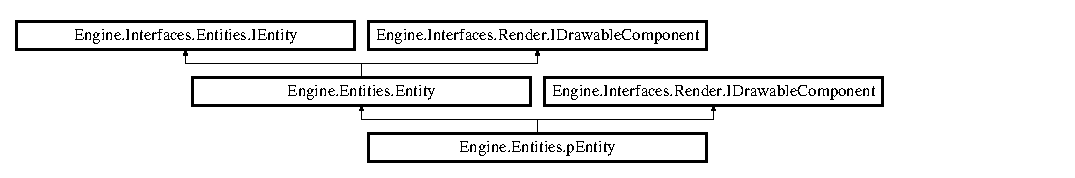
\includegraphics[height=1.944444cm]{de/de9/a00322}
\end{center}
\end{figure}
\subsection*{Public Member Functions}
\begin{DoxyCompactItemize}
\item 
override void \hyperlink{a00322_aad953baa984c0f958d3e96efbfc3bca9}{Initialize} (Vector2 Pos)
\begin{DoxyCompactList}\small\item\em M\+E\+T\+H\+OD\+: Initialise the player by setting it\textquotesingle{}s position and mind \end{DoxyCompactList}\end{DoxyCompactItemize}
\subsection*{Additional Inherited Members}


\subsection{Detailed Description}
C\+L\+A\+SS\+: The player \hyperlink{a00314}{Entity} class 



\subsection{Member Function Documentation}
\mbox{\Hypertarget{a00322_aad953baa984c0f958d3e96efbfc3bca9}\label{a00322_aad953baa984c0f958d3e96efbfc3bca9}} 
\index{Engine\+::\+Entities\+::p\+Entity@{Engine\+::\+Entities\+::p\+Entity}!Initialize@{Initialize}}
\index{Initialize@{Initialize}!Engine\+::\+Entities\+::p\+Entity@{Engine\+::\+Entities\+::p\+Entity}}
\subsubsection{\texorpdfstring{Initialize()}{Initialize()}}
{\footnotesize\ttfamily override void Engine.\+Entities.\+p\+Entity.\+Initialize (\begin{DoxyParamCaption}\item[{Vector2}]{Pos }\end{DoxyParamCaption})\hspace{0.3cm}{\ttfamily [inline]}, {\ttfamily [virtual]}}



M\+E\+T\+H\+OD\+: Initialise the player by setting it\textquotesingle{}s position and mind 


\begin{DoxyParams}{Parameters}
{\em Pos} & \\
\hline
\end{DoxyParams}
S\+ET\+: The mind of this entity using the Service Locator and then Behaviour Manager to create a \hyperlink{a00326}{Player\+Mind}.

C\+A\+LL\+: The Abstract class \hyperlink{a00314}{Entity} Initialise Method.

S\+ET\+: The name of this \hyperlink{a00314}{Entity} to Player. 

Reimplemented from \hyperlink{a00314_aa1425aeeac379c5141e7560b84850b3d}{Engine.\+Entities.\+Entity}.



The documentation for this class was generated from the following file\+:\begin{DoxyCompactItemize}
\item 
\hyperlink{a00023}{p\+Entity.\+cs}\end{DoxyCompactItemize}

\hypertarget{a00326}{}\section{Engine.\+Entities.\+Player\+Mind Class Reference}
\label{a00326}\index{Engine.\+Entities.\+Player\+Mind@{Engine.\+Entities.\+Player\+Mind}}


C\+L\+A\+SS\+: The mind that controls the player \hyperlink{a00314}{Entity}.  


Inheritance diagram for Engine.\+Entities.\+Player\+Mind\+:\begin{figure}[H]
\begin{center}
\leavevmode
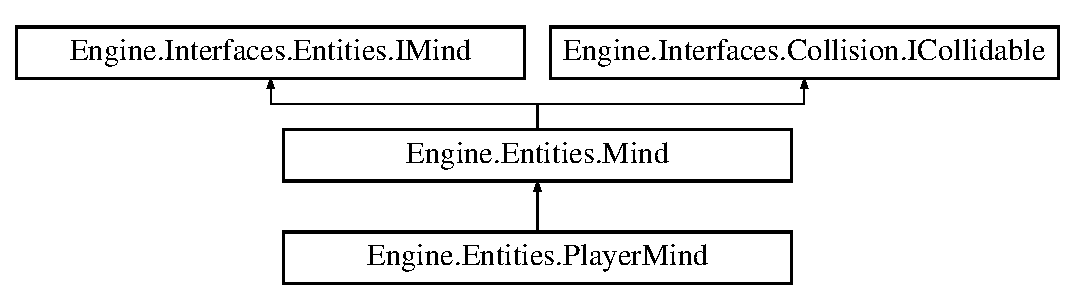
\includegraphics[height=3.000000cm]{d8/d23/a00326}
\end{center}
\end{figure}
\subsection*{Public Member Functions}
\begin{DoxyCompactItemize}
\item 
\hyperlink{a00326_a67a26082f1d70a5c4495cb0ece0cce33}{Player\+Mind} ()
\begin{DoxyCompactList}\small\item\em C\+O\+N\+S\+T\+R\+U\+C\+T\+OR\+: Initialises the basic properties of this object. \end{DoxyCompactList}\item 
override void \hyperlink{a00326_a44a3007533c5d73810c4636fcfef5988}{Initialize} (Vector2 \hyperlink{a00318_ad94b3975c0873fee06b5bd5a75bd38cd}{Position})
\begin{DoxyCompactList}\small\item\em M\+E\+T\+H\+OD\+: Initialise the object and sets properties accordingly. \end{DoxyCompactList}\item 
override void \hyperlink{a00326_a172dca0ea26dfd821b413f7592a98084}{Update} (Game\+Time game\+Time)
\begin{DoxyCompactList}\small\item\em M\+E\+T\+H\+OD\+: Update, controls the behaviour of this object and is looped through every frame. \end{DoxyCompactList}\item 
override void \hyperlink{a00326_a80bacdc33e51129afed33f9e8bd5cd0f}{Unload} ()
\begin{DoxyCompactList}\small\item\em M\+E\+T\+H\+OD\+: Responsible for unloading everything and sending it to the garbage collector to ensure no memory leaks. \end{DoxyCompactList}\item 
void \hyperlink{a00326_a2c9b5d3a4834dc7446584a802460837f}{On\+Key\+Down} (object sender, \hyperlink{a00362}{Key\+Event\+Args} m)
\begin{DoxyCompactList}\small\item\em E\+V\+E\+NT\+: When a key is pressed \end{DoxyCompactList}\item 
void \hyperlink{a00326_ab3295433000f4defc2a420d9758c218e}{On\+Key\+Held} (object sender, \hyperlink{a00362}{Key\+Event\+Args} m)
\begin{DoxyCompactList}\small\item\em E\+V\+E\+NT\+: When a key is held down \end{DoxyCompactList}\item 
void \hyperlink{a00326_a25869d97c0416cc348d589fb423b9d05}{On\+Mouse\+Down} (object sender, \hyperlink{a00374}{Mouse\+Event\+Args} m)
\begin{DoxyCompactList}\small\item\em E\+V\+E\+NT\+: When the mouse is clicked \end{DoxyCompactList}\item 
void \hyperlink{a00326_a008321c6a6ec30ed7ef82f13f6dc6d4e}{On\+Collision} (object sender, \hyperlink{a00350}{Collision\+Event\+Args} cae)
\begin{DoxyCompactList}\small\item\em E\+V\+E\+NT\+: When colliding with another object (A\+A\+BB Collision). \end{DoxyCompactList}\end{DoxyCompactItemize}
\subsection*{Additional Inherited Members}


\subsection{Detailed Description}
C\+L\+A\+SS\+: The mind that controls the player \hyperlink{a00314}{Entity}. 



\subsection{Constructor \& Destructor Documentation}
\mbox{\Hypertarget{a00326_a67a26082f1d70a5c4495cb0ece0cce33}\label{a00326_a67a26082f1d70a5c4495cb0ece0cce33}} 
\index{Engine\+::\+Entities\+::\+Player\+Mind@{Engine\+::\+Entities\+::\+Player\+Mind}!Player\+Mind@{Player\+Mind}}
\index{Player\+Mind@{Player\+Mind}!Engine\+::\+Entities\+::\+Player\+Mind@{Engine\+::\+Entities\+::\+Player\+Mind}}
\subsubsection{\texorpdfstring{Player\+Mind()}{PlayerMind()}}
{\footnotesize\ttfamily Engine.\+Entities.\+Player\+Mind.\+Player\+Mind (\begin{DoxyParamCaption}{ }\end{DoxyParamCaption})\hspace{0.3cm}{\ttfamily [inline]}}



C\+O\+N\+S\+T\+R\+U\+C\+T\+OR\+: Initialises the basic properties of this object. 

S\+ET\+: This is an object that will be used for calculating collision.

C\+R\+E\+A\+TE\+: Event handlers for the behaviour of this object. 

\subsection{Member Function Documentation}
\mbox{\Hypertarget{a00326_a44a3007533c5d73810c4636fcfef5988}\label{a00326_a44a3007533c5d73810c4636fcfef5988}} 
\index{Engine\+::\+Entities\+::\+Player\+Mind@{Engine\+::\+Entities\+::\+Player\+Mind}!Initialize@{Initialize}}
\index{Initialize@{Initialize}!Engine\+::\+Entities\+::\+Player\+Mind@{Engine\+::\+Entities\+::\+Player\+Mind}}
\subsubsection{\texorpdfstring{Initialize()}{Initialize()}}
{\footnotesize\ttfamily override void Engine.\+Entities.\+Player\+Mind.\+Initialize (\begin{DoxyParamCaption}\item[{Vector2}]{Position }\end{DoxyParamCaption})\hspace{0.3cm}{\ttfamily [inline]}, {\ttfamily [virtual]}}



M\+E\+T\+H\+OD\+: Initialise the object and sets properties accordingly. 


\begin{DoxyParams}{Parameters}
{\em Position} & \\
\hline
\end{DoxyParams}
S\+ET\+: the Texture of the entity this controls.

S\+ET\+: The physics properties of this object.

A\+DD\+: The hitboxes of this object.

C\+A\+LL\+: The initialise of the Abstract \hyperlink{a00318}{Mind} class. 

Reimplemented from \hyperlink{a00318_a353d7d2bb1035aefebf0ae3e3f1d1488}{Engine.\+Entities.\+Mind}.

\mbox{\Hypertarget{a00326_a008321c6a6ec30ed7ef82f13f6dc6d4e}\label{a00326_a008321c6a6ec30ed7ef82f13f6dc6d4e}} 
\index{Engine\+::\+Entities\+::\+Player\+Mind@{Engine\+::\+Entities\+::\+Player\+Mind}!On\+Collision@{On\+Collision}}
\index{On\+Collision@{On\+Collision}!Engine\+::\+Entities\+::\+Player\+Mind@{Engine\+::\+Entities\+::\+Player\+Mind}}
\subsubsection{\texorpdfstring{On\+Collision()}{OnCollision()}}
{\footnotesize\ttfamily void Engine.\+Entities.\+Player\+Mind.\+On\+Collision (\begin{DoxyParamCaption}\item[{object}]{sender,  }\item[{\hyperlink{a00350}{Collision\+Event\+Args}}]{cae }\end{DoxyParamCaption})\hspace{0.3cm}{\ttfamily [inline]}}



E\+V\+E\+NT\+: When colliding with another object (A\+A\+BB Collision). 


\begin{DoxyParams}{Parameters}
{\em sender} & \\
\hline
{\em cae} & \\
\hline
\end{DoxyParams}
IF\+: This is object A

S\+ET\+: The object is colliding

A\+DD\+: The minimum translation vector to the position. \mbox{\Hypertarget{a00326_a2c9b5d3a4834dc7446584a802460837f}\label{a00326_a2c9b5d3a4834dc7446584a802460837f}} 
\index{Engine\+::\+Entities\+::\+Player\+Mind@{Engine\+::\+Entities\+::\+Player\+Mind}!On\+Key\+Down@{On\+Key\+Down}}
\index{On\+Key\+Down@{On\+Key\+Down}!Engine\+::\+Entities\+::\+Player\+Mind@{Engine\+::\+Entities\+::\+Player\+Mind}}
\subsubsection{\texorpdfstring{On\+Key\+Down()}{OnKeyDown()}}
{\footnotesize\ttfamily void Engine.\+Entities.\+Player\+Mind.\+On\+Key\+Down (\begin{DoxyParamCaption}\item[{object}]{sender,  }\item[{\hyperlink{a00362}{Key\+Event\+Args}}]{m }\end{DoxyParamCaption})\hspace{0.3cm}{\ttfamily [inline]}}



E\+V\+E\+NT\+: When a key is pressed 


\begin{DoxyParams}{Parameters}
{\em sender} & \\
\hline
{\em m} & \\
\hline
\end{DoxyParams}
\mbox{\Hypertarget{a00326_ab3295433000f4defc2a420d9758c218e}\label{a00326_ab3295433000f4defc2a420d9758c218e}} 
\index{Engine\+::\+Entities\+::\+Player\+Mind@{Engine\+::\+Entities\+::\+Player\+Mind}!On\+Key\+Held@{On\+Key\+Held}}
\index{On\+Key\+Held@{On\+Key\+Held}!Engine\+::\+Entities\+::\+Player\+Mind@{Engine\+::\+Entities\+::\+Player\+Mind}}
\subsubsection{\texorpdfstring{On\+Key\+Held()}{OnKeyHeld()}}
{\footnotesize\ttfamily void Engine.\+Entities.\+Player\+Mind.\+On\+Key\+Held (\begin{DoxyParamCaption}\item[{object}]{sender,  }\item[{\hyperlink{a00362}{Key\+Event\+Args}}]{m }\end{DoxyParamCaption})\hspace{0.3cm}{\ttfamily [inline]}}



E\+V\+E\+NT\+: When a key is held down 


\begin{DoxyParams}{Parameters}
{\em sender} & \\
\hline
{\em m} & \\
\hline
\end{DoxyParams}
I\+N\+I\+T\+I\+A\+L\+I\+SE\+: An array of keys on the keyboard that are pressed and held

IF\+: D is held

C\+A\+LL\+: Apply Force in the right direction

IF\+: A is held

C\+A\+LL\+: Apply force in the left direction

IF\+: S is held

C\+A\+LL\+: Apply force in the down direction

IF\+: W is held

C\+A\+LL\+: Apply force in the up direction \mbox{\Hypertarget{a00326_a25869d97c0416cc348d589fb423b9d05}\label{a00326_a25869d97c0416cc348d589fb423b9d05}} 
\index{Engine\+::\+Entities\+::\+Player\+Mind@{Engine\+::\+Entities\+::\+Player\+Mind}!On\+Mouse\+Down@{On\+Mouse\+Down}}
\index{On\+Mouse\+Down@{On\+Mouse\+Down}!Engine\+::\+Entities\+::\+Player\+Mind@{Engine\+::\+Entities\+::\+Player\+Mind}}
\subsubsection{\texorpdfstring{On\+Mouse\+Down()}{OnMouseDown()}}
{\footnotesize\ttfamily void Engine.\+Entities.\+Player\+Mind.\+On\+Mouse\+Down (\begin{DoxyParamCaption}\item[{object}]{sender,  }\item[{\hyperlink{a00374}{Mouse\+Event\+Args}}]{m }\end{DoxyParamCaption})\hspace{0.3cm}{\ttfamily [inline]}}



E\+V\+E\+NT\+: When the mouse is clicked 


\begin{DoxyParams}{Parameters}
{\em sender} & \\
\hline
{\em m} & \\
\hline
\end{DoxyParams}
\mbox{\Hypertarget{a00326_a80bacdc33e51129afed33f9e8bd5cd0f}\label{a00326_a80bacdc33e51129afed33f9e8bd5cd0f}} 
\index{Engine\+::\+Entities\+::\+Player\+Mind@{Engine\+::\+Entities\+::\+Player\+Mind}!Unload@{Unload}}
\index{Unload@{Unload}!Engine\+::\+Entities\+::\+Player\+Mind@{Engine\+::\+Entities\+::\+Player\+Mind}}
\subsubsection{\texorpdfstring{Unload()}{Unload()}}
{\footnotesize\ttfamily override void Engine.\+Entities.\+Player\+Mind.\+Unload (\begin{DoxyParamCaption}{ }\end{DoxyParamCaption})\hspace{0.3cm}{\ttfamily [inline]}, {\ttfamily [virtual]}}



M\+E\+T\+H\+OD\+: Responsible for unloading everything and sending it to the garbage collector to ensure no memory leaks. 



Reimplemented from \hyperlink{a00318_a15bf25a4a74706ef37592689f43c0598}{Engine.\+Entities.\+Mind}.

\mbox{\Hypertarget{a00326_a172dca0ea26dfd821b413f7592a98084}\label{a00326_a172dca0ea26dfd821b413f7592a98084}} 
\index{Engine\+::\+Entities\+::\+Player\+Mind@{Engine\+::\+Entities\+::\+Player\+Mind}!Update@{Update}}
\index{Update@{Update}!Engine\+::\+Entities\+::\+Player\+Mind@{Engine\+::\+Entities\+::\+Player\+Mind}}
\subsubsection{\texorpdfstring{Update()}{Update()}}
{\footnotesize\ttfamily override void Engine.\+Entities.\+Player\+Mind.\+Update (\begin{DoxyParamCaption}\item[{Game\+Time}]{game\+Time }\end{DoxyParamCaption})\hspace{0.3cm}{\ttfamily [inline]}, {\ttfamily [virtual]}}



M\+E\+T\+H\+OD\+: Update, controls the behaviour of this object and is looped through every frame. 


\begin{DoxyParams}{Parameters}
{\em game\+Time} & \\
\hline
\end{DoxyParams}
C\+A\+LL\+: The update\+Physics method which controls the physical simulation of movement of the object.

C\+A\+LL\+: the update method of the abstract mind class. 

Reimplemented from \hyperlink{a00318_adec6999d87accf7371de1536eac2541b}{Engine.\+Entities.\+Mind}.



The documentation for this class was generated from the following file\+:\begin{DoxyCompactItemize}
\item 
\hyperlink{a00026}{Player\+Mind.\+cs}\end{DoxyCompactItemize}

\hypertarget{a00526}{}\section{Engine.\+Managers.\+Render.\+Render\+Manager Class Reference}
\label{a00526}\index{Engine.\+Managers.\+Render.\+Render\+Manager@{Engine.\+Managers.\+Render.\+Render\+Manager}}


C\+L\+A\+SS\+: The \hyperlink{a00271}{Render} manager is responsible for the drawing of content loaded by the various other managers  


Inheritance diagram for Engine.\+Managers.\+Render.\+Render\+Manager\+:\begin{figure}[H]
\begin{center}
\leavevmode
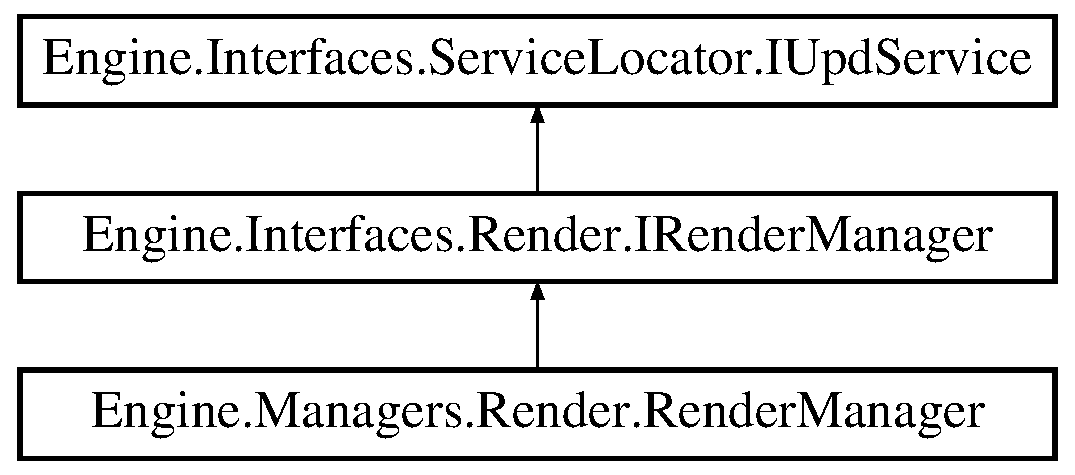
\includegraphics[height=3.000000cm]{d0/d35/a00526}
\end{center}
\end{figure}
\subsection*{Public Member Functions}
\begin{DoxyCompactItemize}
\item 
\hyperlink{a00526_a0ecca32f070bd247added2b680fe390d}{Render\+Manager} ()
\begin{DoxyCompactList}\small\item\em C\+O\+N\+S\+T\+R\+U\+C\+T\+OR \end{DoxyCompactList}\item 
void \hyperlink{a00526_abd794ae4c12392323e9afda73e459bef}{Initialize} ()
\begin{DoxyCompactList}\small\item\em M\+E\+T\+H\+OD\+: An initialize method that is called every time a new screen is ready to be drawn \end{DoxyCompactList}\item 
void \hyperlink{a00526_aeb436300e604d81ff837227e5dd11710}{get\+Entity\+List} ()
\begin{DoxyCompactList}\small\item\em M\+E\+T\+H\+OD\+: gets the entity list from the Entity Manager \end{DoxyCompactList}\item 
void \hyperlink{a00526_a79fb84c735ca8b863eed41f51566f554}{get\+Cam\+Entity\+List} ()
\begin{DoxyCompactList}\small\item\em M\+E\+T\+H\+OD\+: gets the entity list from the Entity Manager \end{DoxyCompactList}\item 
void \hyperlink{a00526_a6f4d9756fcf88b78263f0bc5538b1912}{add\+Drawable} (\hyperlink{a00454}{I\+Drawable\+Component} d)
\begin{DoxyCompactList}\small\item\em M\+E\+T\+H\+OD\+: For items which dont wish to be drawn in regards to the cameras matrix translations (such as G\+UI) \end{DoxyCompactList}\item 
void \hyperlink{a00526_abe4458f6b030cffba170149d1ee63bba}{add\+Cam\+Drawable} (\hyperlink{a00454}{I\+Drawable\+Component} d)
\begin{DoxyCompactList}\small\item\em M\+E\+T\+H\+OD\+: For Scenery/\+Entities which wish to be drawn in regards to the cameras matrix translations \end{DoxyCompactList}\item 
void \hyperlink{a00526_a9b6bcc0390e87b334c36c1083e0af5f6}{add\+Cam\+Draw\+Entity} (\hyperlink{a00454}{I\+Drawable\+Component} d)
\begin{DoxyCompactList}\small\item\em M\+E\+T\+H\+OD\+: For \hyperlink{a00269}{Entities} which wish to be drawn in regards to the cameras matrix translations \end{DoxyCompactList}\item 
void \hyperlink{a00526_a93c2cea1133bb38a01336b3d4c6b0321}{Draw\+Camera\+Related\+Artefacts} ()
\begin{DoxyCompactList}\small\item\em M\+E\+T\+H\+OD\+: Draws everything in the camera view \end{DoxyCompactList}\item 
void \hyperlink{a00526_af77caeb94739b508306100cdedfcbd9b}{clear\+Temp\+Entity} ()
\begin{DoxyCompactList}\small\item\em M\+E\+T\+H\+OD\+: Clears the entities to be drawn in relation to the camera \end{DoxyCompactList}\item 
void \hyperlink{a00526_a0dfca7db5472741f87837e7f87e90129}{Draw\+Non\+Camera\+Related\+Artefacts} ()
\begin{DoxyCompactList}\small\item\em M\+E\+T\+H\+OD\+: Draws everything not related to the camera \end{DoxyCompactList}\item 
void \hyperlink{a00526_a9ce9959462da544f283ab3e531bd1edb}{add\+String} (\hyperlink{a00598}{Game\+Text} game\+Text)
\item 
void \hyperlink{a00526_a9d572b8cd8ba3c6cac622dee8d14f2a1}{add\+Shape} (\hyperlink{a00454}{I\+Drawable\+Component} shape)
\item 
void \hyperlink{a00526_a7b63b947d986ab05b66c4c9f78ee3c20}{Update} (Game\+Time game\+Time)
\begin{DoxyCompactList}\small\item\em M\+E\+T\+H\+OD\+: The update loop cycled through on each frame \end{DoxyCompactList}\item 
void \hyperlink{a00526_ae9fd08da224435b71540e67f718eb7c4}{Draw} ()
\begin{DoxyCompactList}\small\item\em M\+E\+T\+H\+OD\+: Draws items \end{DoxyCompactList}\item 
void \hyperlink{a00526_a5e7f7ef9bf468db27267ee1e50a34af3}{Draw} (Texture2D texture, Rectangle rect, Color col)
\begin{DoxyCompactList}\small\item\em M\+E\+T\+H\+OD\+: Draws items \end{DoxyCompactList}\item 
void \hyperlink{a00526_a9eb548f058744b031b639810a16ba40d}{Draw\+Entities} ()
\item 
void \hyperlink{a00526_a0df839a3a677b7595e4535716e823809}{Draw\+Components} ()
\item 
void \hyperlink{a00526_af81e4faf42327afbf604c3bb4d09499a}{Draw\+Shapes} ()
\item 
void \hyperlink{a00526_aa957794d6537025fb2535517bcc691cc}{Draw\+Drawables} ()
\begin{DoxyCompactList}\small\item\em M\+E\+T\+H\+OD\+: Draws every Drawable object \end{DoxyCompactList}\item 
void \hyperlink{a00526_adc520b6c317ed9e0d4e51fd34c22c511}{Draw\+Cam\+Drawables} ()
\begin{DoxyCompactList}\small\item\em M\+E\+T\+H\+OD\+: D\+Raws everything in relation to the camera \end{DoxyCompactList}\item 
void \hyperlink{a00526_a96510018c93924e8d5456891b28b51bb}{Draw\+Cam\+Draw\+Entities} ()
\begin{DoxyCompactList}\small\item\em M\+E\+T\+H\+OD\+: draws entities in relation to the camera \end{DoxyCompactList}\end{DoxyCompactItemize}
\subsection*{Properties}
\begin{DoxyCompactItemize}
\item 
Sprite\+Batch \hyperlink{a00526_afd06d1ef067613ca63fe1302c4c41e3d}{sprite\+Batch}\hspace{0.3cm}{\ttfamily  \mbox{[}get, set\mbox{]}}
\item 
List$<$ \hyperlink{a00454}{I\+Drawable\+Component} $>$ \hyperlink{a00526_a954e0be8a74a97fd978b65edba1c0223}{getD}\hspace{0.3cm}{\ttfamily  \mbox{[}get\mbox{]}}
\item 
List$<$ \hyperlink{a00454}{I\+Drawable\+Component} $>$ \hyperlink{a00526_afb8e15ee3c1d4f62a0ed4b60f433199e}{get\+D1}\hspace{0.3cm}{\ttfamily  \mbox{[}get\mbox{]}}
\end{DoxyCompactItemize}


\subsection{Detailed Description}
C\+L\+A\+SS\+: The \hyperlink{a00271}{Render} manager is responsible for the drawing of content loaded by the various other managers 



\subsection{Constructor \& Destructor Documentation}
\mbox{\Hypertarget{a00526_a0ecca32f070bd247added2b680fe390d}\label{a00526_a0ecca32f070bd247added2b680fe390d}} 
\index{Engine\+::\+Managers\+::\+Render\+::\+Render\+Manager@{Engine\+::\+Managers\+::\+Render\+::\+Render\+Manager}!Render\+Manager@{Render\+Manager}}
\index{Render\+Manager@{Render\+Manager}!Engine\+::\+Managers\+::\+Render\+::\+Render\+Manager@{Engine\+::\+Managers\+::\+Render\+::\+Render\+Manager}}
\subsubsection{\texorpdfstring{Render\+Manager()}{RenderManager()}}
{\footnotesize\ttfamily Engine.\+Managers.\+Render.\+Render\+Manager.\+Render\+Manager (\begin{DoxyParamCaption}{ }\end{DoxyParamCaption})\hspace{0.3cm}{\ttfamily [inline]}}



C\+O\+N\+S\+T\+R\+U\+C\+T\+OR 



\subsection{Member Function Documentation}
\mbox{\Hypertarget{a00526_abe4458f6b030cffba170149d1ee63bba}\label{a00526_abe4458f6b030cffba170149d1ee63bba}} 
\index{Engine\+::\+Managers\+::\+Render\+::\+Render\+Manager@{Engine\+::\+Managers\+::\+Render\+::\+Render\+Manager}!add\+Cam\+Drawable@{add\+Cam\+Drawable}}
\index{add\+Cam\+Drawable@{add\+Cam\+Drawable}!Engine\+::\+Managers\+::\+Render\+::\+Render\+Manager@{Engine\+::\+Managers\+::\+Render\+::\+Render\+Manager}}
\subsubsection{\texorpdfstring{add\+Cam\+Drawable()}{addCamDrawable()}}
{\footnotesize\ttfamily void Engine.\+Managers.\+Render.\+Render\+Manager.\+add\+Cam\+Drawable (\begin{DoxyParamCaption}\item[{\hyperlink{a00454}{I\+Drawable\+Component}}]{d }\end{DoxyParamCaption})\hspace{0.3cm}{\ttfamily [inline]}}



M\+E\+T\+H\+OD\+: For Scenery/\+Entities which wish to be drawn in regards to the cameras matrix translations 


\begin{DoxyParams}{Parameters}
{\em d} & the object to be drawn\\
\hline
\end{DoxyParams}


Implements \hyperlink{a00458_a85d74d22976a3d818b21cc856da85092}{Engine.\+Interfaces.\+Render.\+I\+Render\+Manager}.

\mbox{\Hypertarget{a00526_a9b6bcc0390e87b334c36c1083e0af5f6}\label{a00526_a9b6bcc0390e87b334c36c1083e0af5f6}} 
\index{Engine\+::\+Managers\+::\+Render\+::\+Render\+Manager@{Engine\+::\+Managers\+::\+Render\+::\+Render\+Manager}!add\+Cam\+Draw\+Entity@{add\+Cam\+Draw\+Entity}}
\index{add\+Cam\+Draw\+Entity@{add\+Cam\+Draw\+Entity}!Engine\+::\+Managers\+::\+Render\+::\+Render\+Manager@{Engine\+::\+Managers\+::\+Render\+::\+Render\+Manager}}
\subsubsection{\texorpdfstring{add\+Cam\+Draw\+Entity()}{addCamDrawEntity()}}
{\footnotesize\ttfamily void Engine.\+Managers.\+Render.\+Render\+Manager.\+add\+Cam\+Draw\+Entity (\begin{DoxyParamCaption}\item[{\hyperlink{a00454}{I\+Drawable\+Component}}]{d }\end{DoxyParamCaption})\hspace{0.3cm}{\ttfamily [inline]}}



M\+E\+T\+H\+OD\+: For \hyperlink{a00269}{Entities} which wish to be drawn in regards to the cameras matrix translations 


\begin{DoxyParams}{Parameters}
{\em d} & The object to be drawn\\
\hline
\end{DoxyParams}


Implements \hyperlink{a00458_a5ce82555229026255b46d824edc679e8}{Engine.\+Interfaces.\+Render.\+I\+Render\+Manager}.

\mbox{\Hypertarget{a00526_a6f4d9756fcf88b78263f0bc5538b1912}\label{a00526_a6f4d9756fcf88b78263f0bc5538b1912}} 
\index{Engine\+::\+Managers\+::\+Render\+::\+Render\+Manager@{Engine\+::\+Managers\+::\+Render\+::\+Render\+Manager}!add\+Drawable@{add\+Drawable}}
\index{add\+Drawable@{add\+Drawable}!Engine\+::\+Managers\+::\+Render\+::\+Render\+Manager@{Engine\+::\+Managers\+::\+Render\+::\+Render\+Manager}}
\subsubsection{\texorpdfstring{add\+Drawable()}{addDrawable()}}
{\footnotesize\ttfamily void Engine.\+Managers.\+Render.\+Render\+Manager.\+add\+Drawable (\begin{DoxyParamCaption}\item[{\hyperlink{a00454}{I\+Drawable\+Component}}]{d }\end{DoxyParamCaption})\hspace{0.3cm}{\ttfamily [inline]}}



M\+E\+T\+H\+OD\+: For items which dont wish to be drawn in regards to the cameras matrix translations (such as G\+UI) 


\begin{DoxyParams}{Parameters}
{\em d} & The object to be drawn\\
\hline
\end{DoxyParams}


Implements \hyperlink{a00458_a3beadf9574678e62c968c8631b367348}{Engine.\+Interfaces.\+Render.\+I\+Render\+Manager}.

\mbox{\Hypertarget{a00526_a9d572b8cd8ba3c6cac622dee8d14f2a1}\label{a00526_a9d572b8cd8ba3c6cac622dee8d14f2a1}} 
\index{Engine\+::\+Managers\+::\+Render\+::\+Render\+Manager@{Engine\+::\+Managers\+::\+Render\+::\+Render\+Manager}!add\+Shape@{add\+Shape}}
\index{add\+Shape@{add\+Shape}!Engine\+::\+Managers\+::\+Render\+::\+Render\+Manager@{Engine\+::\+Managers\+::\+Render\+::\+Render\+Manager}}
\subsubsection{\texorpdfstring{add\+Shape()}{addShape()}}
{\footnotesize\ttfamily void Engine.\+Managers.\+Render.\+Render\+Manager.\+add\+Shape (\begin{DoxyParamCaption}\item[{\hyperlink{a00454}{I\+Drawable\+Component}}]{shape }\end{DoxyParamCaption})\hspace{0.3cm}{\ttfamily [inline]}}



Implements \hyperlink{a00458_a89bf09f0f2d6144e68cd045d39f13374}{Engine.\+Interfaces.\+Render.\+I\+Render\+Manager}.

\mbox{\Hypertarget{a00526_a9ce9959462da544f283ab3e531bd1edb}\label{a00526_a9ce9959462da544f283ab3e531bd1edb}} 
\index{Engine\+::\+Managers\+::\+Render\+::\+Render\+Manager@{Engine\+::\+Managers\+::\+Render\+::\+Render\+Manager}!add\+String@{add\+String}}
\index{add\+String@{add\+String}!Engine\+::\+Managers\+::\+Render\+::\+Render\+Manager@{Engine\+::\+Managers\+::\+Render\+::\+Render\+Manager}}
\subsubsection{\texorpdfstring{add\+String()}{addString()}}
{\footnotesize\ttfamily void Engine.\+Managers.\+Render.\+Render\+Manager.\+add\+String (\begin{DoxyParamCaption}\item[{\hyperlink{a00598}{Game\+Text}}]{game\+Text }\end{DoxyParamCaption})\hspace{0.3cm}{\ttfamily [inline]}}



Implements \hyperlink{a00458_ae3d8ed9fc1406b62e04ac8336e4e40b3}{Engine.\+Interfaces.\+Render.\+I\+Render\+Manager}.

\mbox{\Hypertarget{a00526_af77caeb94739b508306100cdedfcbd9b}\label{a00526_af77caeb94739b508306100cdedfcbd9b}} 
\index{Engine\+::\+Managers\+::\+Render\+::\+Render\+Manager@{Engine\+::\+Managers\+::\+Render\+::\+Render\+Manager}!clear\+Temp\+Entity@{clear\+Temp\+Entity}}
\index{clear\+Temp\+Entity@{clear\+Temp\+Entity}!Engine\+::\+Managers\+::\+Render\+::\+Render\+Manager@{Engine\+::\+Managers\+::\+Render\+::\+Render\+Manager}}
\subsubsection{\texorpdfstring{clear\+Temp\+Entity()}{clearTempEntity()}}
{\footnotesize\ttfamily void Engine.\+Managers.\+Render.\+Render\+Manager.\+clear\+Temp\+Entity (\begin{DoxyParamCaption}{ }\end{DoxyParamCaption})\hspace{0.3cm}{\ttfamily [inline]}}



M\+E\+T\+H\+OD\+: Clears the entities to be drawn in relation to the camera 



Implements \hyperlink{a00458_a7879b28e310859cdebdc2c8aeaced6b3}{Engine.\+Interfaces.\+Render.\+I\+Render\+Manager}.

\mbox{\Hypertarget{a00526_ae9fd08da224435b71540e67f718eb7c4}\label{a00526_ae9fd08da224435b71540e67f718eb7c4}} 
\index{Engine\+::\+Managers\+::\+Render\+::\+Render\+Manager@{Engine\+::\+Managers\+::\+Render\+::\+Render\+Manager}!Draw@{Draw}}
\index{Draw@{Draw}!Engine\+::\+Managers\+::\+Render\+::\+Render\+Manager@{Engine\+::\+Managers\+::\+Render\+::\+Render\+Manager}}
\subsubsection{\texorpdfstring{Draw()}{Draw()}\hspace{0.1cm}{\footnotesize\ttfamily [1/2]}}
{\footnotesize\ttfamily void Engine.\+Managers.\+Render.\+Render\+Manager.\+Draw (\begin{DoxyParamCaption}{ }\end{DoxyParamCaption})\hspace{0.3cm}{\ttfamily [inline]}}



M\+E\+T\+H\+OD\+: Draws items 



Implements \hyperlink{a00458_afac9eb0644db9971494332e7d179bbf9}{Engine.\+Interfaces.\+Render.\+I\+Render\+Manager}.

\mbox{\Hypertarget{a00526_a5e7f7ef9bf468db27267ee1e50a34af3}\label{a00526_a5e7f7ef9bf468db27267ee1e50a34af3}} 
\index{Engine\+::\+Managers\+::\+Render\+::\+Render\+Manager@{Engine\+::\+Managers\+::\+Render\+::\+Render\+Manager}!Draw@{Draw}}
\index{Draw@{Draw}!Engine\+::\+Managers\+::\+Render\+::\+Render\+Manager@{Engine\+::\+Managers\+::\+Render\+::\+Render\+Manager}}
\subsubsection{\texorpdfstring{Draw()}{Draw()}\hspace{0.1cm}{\footnotesize\ttfamily [2/2]}}
{\footnotesize\ttfamily void Engine.\+Managers.\+Render.\+Render\+Manager.\+Draw (\begin{DoxyParamCaption}\item[{Texture2D}]{texture,  }\item[{Rectangle}]{rect,  }\item[{Color}]{col }\end{DoxyParamCaption})\hspace{0.3cm}{\ttfamily [inline]}}



M\+E\+T\+H\+OD\+: Draws items 



Implements \hyperlink{a00458_ad9f875208c0f901d3e90facfea2acfc0}{Engine.\+Interfaces.\+Render.\+I\+Render\+Manager}.

\mbox{\Hypertarget{a00526_adc520b6c317ed9e0d4e51fd34c22c511}\label{a00526_adc520b6c317ed9e0d4e51fd34c22c511}} 
\index{Engine\+::\+Managers\+::\+Render\+::\+Render\+Manager@{Engine\+::\+Managers\+::\+Render\+::\+Render\+Manager}!Draw\+Cam\+Drawables@{Draw\+Cam\+Drawables}}
\index{Draw\+Cam\+Drawables@{Draw\+Cam\+Drawables}!Engine\+::\+Managers\+::\+Render\+::\+Render\+Manager@{Engine\+::\+Managers\+::\+Render\+::\+Render\+Manager}}
\subsubsection{\texorpdfstring{Draw\+Cam\+Drawables()}{DrawCamDrawables()}}
{\footnotesize\ttfamily void Engine.\+Managers.\+Render.\+Render\+Manager.\+Draw\+Cam\+Drawables (\begin{DoxyParamCaption}{ }\end{DoxyParamCaption})\hspace{0.3cm}{\ttfamily [inline]}}



M\+E\+T\+H\+OD\+: D\+Raws everything in relation to the camera 



Implements \hyperlink{a00458_a9239479d4d4f220b334722e48acb5bc2}{Engine.\+Interfaces.\+Render.\+I\+Render\+Manager}.

\mbox{\Hypertarget{a00526_a96510018c93924e8d5456891b28b51bb}\label{a00526_a96510018c93924e8d5456891b28b51bb}} 
\index{Engine\+::\+Managers\+::\+Render\+::\+Render\+Manager@{Engine\+::\+Managers\+::\+Render\+::\+Render\+Manager}!Draw\+Cam\+Draw\+Entities@{Draw\+Cam\+Draw\+Entities}}
\index{Draw\+Cam\+Draw\+Entities@{Draw\+Cam\+Draw\+Entities}!Engine\+::\+Managers\+::\+Render\+::\+Render\+Manager@{Engine\+::\+Managers\+::\+Render\+::\+Render\+Manager}}
\subsubsection{\texorpdfstring{Draw\+Cam\+Draw\+Entities()}{DrawCamDrawEntities()}}
{\footnotesize\ttfamily void Engine.\+Managers.\+Render.\+Render\+Manager.\+Draw\+Cam\+Draw\+Entities (\begin{DoxyParamCaption}{ }\end{DoxyParamCaption})\hspace{0.3cm}{\ttfamily [inline]}}



M\+E\+T\+H\+OD\+: draws entities in relation to the camera 



Implements \hyperlink{a00458_a521ac08ccb20d1dbe58ff906fc7c42a4}{Engine.\+Interfaces.\+Render.\+I\+Render\+Manager}.

\mbox{\Hypertarget{a00526_a93c2cea1133bb38a01336b3d4c6b0321}\label{a00526_a93c2cea1133bb38a01336b3d4c6b0321}} 
\index{Engine\+::\+Managers\+::\+Render\+::\+Render\+Manager@{Engine\+::\+Managers\+::\+Render\+::\+Render\+Manager}!Draw\+Camera\+Related\+Artefacts@{Draw\+Camera\+Related\+Artefacts}}
\index{Draw\+Camera\+Related\+Artefacts@{Draw\+Camera\+Related\+Artefacts}!Engine\+::\+Managers\+::\+Render\+::\+Render\+Manager@{Engine\+::\+Managers\+::\+Render\+::\+Render\+Manager}}
\subsubsection{\texorpdfstring{Draw\+Camera\+Related\+Artefacts()}{DrawCameraRelatedArtefacts()}}
{\footnotesize\ttfamily void Engine.\+Managers.\+Render.\+Render\+Manager.\+Draw\+Camera\+Related\+Artefacts (\begin{DoxyParamCaption}{ }\end{DoxyParamCaption})\hspace{0.3cm}{\ttfamily [inline]}}



M\+E\+T\+H\+OD\+: Draws everything in the camera view 

Below method should be in noncamera 

Implements \hyperlink{a00458_aee587a69646dc58e02ba4430f1368bf0}{Engine.\+Interfaces.\+Render.\+I\+Render\+Manager}.

\mbox{\Hypertarget{a00526_a0df839a3a677b7595e4535716e823809}\label{a00526_a0df839a3a677b7595e4535716e823809}} 
\index{Engine\+::\+Managers\+::\+Render\+::\+Render\+Manager@{Engine\+::\+Managers\+::\+Render\+::\+Render\+Manager}!Draw\+Components@{Draw\+Components}}
\index{Draw\+Components@{Draw\+Components}!Engine\+::\+Managers\+::\+Render\+::\+Render\+Manager@{Engine\+::\+Managers\+::\+Render\+::\+Render\+Manager}}
\subsubsection{\texorpdfstring{Draw\+Components()}{DrawComponents()}}
{\footnotesize\ttfamily void Engine.\+Managers.\+Render.\+Render\+Manager.\+Draw\+Components (\begin{DoxyParamCaption}{ }\end{DoxyParamCaption})\hspace{0.3cm}{\ttfamily [inline]}}



Implements \hyperlink{a00458_a326852d43fb14fb872d856ff2c1d6fd9}{Engine.\+Interfaces.\+Render.\+I\+Render\+Manager}.

\mbox{\Hypertarget{a00526_aa957794d6537025fb2535517bcc691cc}\label{a00526_aa957794d6537025fb2535517bcc691cc}} 
\index{Engine\+::\+Managers\+::\+Render\+::\+Render\+Manager@{Engine\+::\+Managers\+::\+Render\+::\+Render\+Manager}!Draw\+Drawables@{Draw\+Drawables}}
\index{Draw\+Drawables@{Draw\+Drawables}!Engine\+::\+Managers\+::\+Render\+::\+Render\+Manager@{Engine\+::\+Managers\+::\+Render\+::\+Render\+Manager}}
\subsubsection{\texorpdfstring{Draw\+Drawables()}{DrawDrawables()}}
{\footnotesize\ttfamily void Engine.\+Managers.\+Render.\+Render\+Manager.\+Draw\+Drawables (\begin{DoxyParamCaption}{ }\end{DoxyParamCaption})\hspace{0.3cm}{\ttfamily [inline]}}



M\+E\+T\+H\+OD\+: Draws every Drawable object 



Implements \hyperlink{a00458_ace0e8fa7ce70c3437fce1298b22bf195}{Engine.\+Interfaces.\+Render.\+I\+Render\+Manager}.

\mbox{\Hypertarget{a00526_a9eb548f058744b031b639810a16ba40d}\label{a00526_a9eb548f058744b031b639810a16ba40d}} 
\index{Engine\+::\+Managers\+::\+Render\+::\+Render\+Manager@{Engine\+::\+Managers\+::\+Render\+::\+Render\+Manager}!Draw\+Entities@{Draw\+Entities}}
\index{Draw\+Entities@{Draw\+Entities}!Engine\+::\+Managers\+::\+Render\+::\+Render\+Manager@{Engine\+::\+Managers\+::\+Render\+::\+Render\+Manager}}
\subsubsection{\texorpdfstring{Draw\+Entities()}{DrawEntities()}}
{\footnotesize\ttfamily void Engine.\+Managers.\+Render.\+Render\+Manager.\+Draw\+Entities (\begin{DoxyParamCaption}{ }\end{DoxyParamCaption})\hspace{0.3cm}{\ttfamily [inline]}}



Implements \hyperlink{a00458_aa7c35d67893f29738baab63370d16b10}{Engine.\+Interfaces.\+Render.\+I\+Render\+Manager}.

\mbox{\Hypertarget{a00526_a0dfca7db5472741f87837e7f87e90129}\label{a00526_a0dfca7db5472741f87837e7f87e90129}} 
\index{Engine\+::\+Managers\+::\+Render\+::\+Render\+Manager@{Engine\+::\+Managers\+::\+Render\+::\+Render\+Manager}!Draw\+Non\+Camera\+Related\+Artefacts@{Draw\+Non\+Camera\+Related\+Artefacts}}
\index{Draw\+Non\+Camera\+Related\+Artefacts@{Draw\+Non\+Camera\+Related\+Artefacts}!Engine\+::\+Managers\+::\+Render\+::\+Render\+Manager@{Engine\+::\+Managers\+::\+Render\+::\+Render\+Manager}}
\subsubsection{\texorpdfstring{Draw\+Non\+Camera\+Related\+Artefacts()}{DrawNonCameraRelatedArtefacts()}}
{\footnotesize\ttfamily void Engine.\+Managers.\+Render.\+Render\+Manager.\+Draw\+Non\+Camera\+Related\+Artefacts (\begin{DoxyParamCaption}{ }\end{DoxyParamCaption})\hspace{0.3cm}{\ttfamily [inline]}}



M\+E\+T\+H\+OD\+: Draws everything not related to the camera 



Implements \hyperlink{a00458_a566b23b9d0b60e2fb06107e7a6c239cb}{Engine.\+Interfaces.\+Render.\+I\+Render\+Manager}.

\mbox{\Hypertarget{a00526_af81e4faf42327afbf604c3bb4d09499a}\label{a00526_af81e4faf42327afbf604c3bb4d09499a}} 
\index{Engine\+::\+Managers\+::\+Render\+::\+Render\+Manager@{Engine\+::\+Managers\+::\+Render\+::\+Render\+Manager}!Draw\+Shapes@{Draw\+Shapes}}
\index{Draw\+Shapes@{Draw\+Shapes}!Engine\+::\+Managers\+::\+Render\+::\+Render\+Manager@{Engine\+::\+Managers\+::\+Render\+::\+Render\+Manager}}
\subsubsection{\texorpdfstring{Draw\+Shapes()}{DrawShapes()}}
{\footnotesize\ttfamily void Engine.\+Managers.\+Render.\+Render\+Manager.\+Draw\+Shapes (\begin{DoxyParamCaption}{ }\end{DoxyParamCaption})\hspace{0.3cm}{\ttfamily [inline]}}



Implements \hyperlink{a00458_af785d8e5292f1f8f89c47d300e2c7d67}{Engine.\+Interfaces.\+Render.\+I\+Render\+Manager}.

\mbox{\Hypertarget{a00526_a79fb84c735ca8b863eed41f51566f554}\label{a00526_a79fb84c735ca8b863eed41f51566f554}} 
\index{Engine\+::\+Managers\+::\+Render\+::\+Render\+Manager@{Engine\+::\+Managers\+::\+Render\+::\+Render\+Manager}!get\+Cam\+Entity\+List@{get\+Cam\+Entity\+List}}
\index{get\+Cam\+Entity\+List@{get\+Cam\+Entity\+List}!Engine\+::\+Managers\+::\+Render\+::\+Render\+Manager@{Engine\+::\+Managers\+::\+Render\+::\+Render\+Manager}}
\subsubsection{\texorpdfstring{get\+Cam\+Entity\+List()}{getCamEntityList()}}
{\footnotesize\ttfamily void Engine.\+Managers.\+Render.\+Render\+Manager.\+get\+Cam\+Entity\+List (\begin{DoxyParamCaption}{ }\end{DoxyParamCaption})\hspace{0.3cm}{\ttfamily [inline]}}



M\+E\+T\+H\+OD\+: gets the entity list from the Entity Manager 



Implements \hyperlink{a00458_a37f1fdeb82edc4e414404d43d1c6bb51}{Engine.\+Interfaces.\+Render.\+I\+Render\+Manager}.

\mbox{\Hypertarget{a00526_aeb436300e604d81ff837227e5dd11710}\label{a00526_aeb436300e604d81ff837227e5dd11710}} 
\index{Engine\+::\+Managers\+::\+Render\+::\+Render\+Manager@{Engine\+::\+Managers\+::\+Render\+::\+Render\+Manager}!get\+Entity\+List@{get\+Entity\+List}}
\index{get\+Entity\+List@{get\+Entity\+List}!Engine\+::\+Managers\+::\+Render\+::\+Render\+Manager@{Engine\+::\+Managers\+::\+Render\+::\+Render\+Manager}}
\subsubsection{\texorpdfstring{get\+Entity\+List()}{getEntityList()}}
{\footnotesize\ttfamily void Engine.\+Managers.\+Render.\+Render\+Manager.\+get\+Entity\+List (\begin{DoxyParamCaption}{ }\end{DoxyParamCaption})\hspace{0.3cm}{\ttfamily [inline]}}



M\+E\+T\+H\+OD\+: gets the entity list from the Entity Manager 



Implements \hyperlink{a00458_a48c8e64f7e597fdea8412057d24bcb3d}{Engine.\+Interfaces.\+Render.\+I\+Render\+Manager}.

\mbox{\Hypertarget{a00526_abd794ae4c12392323e9afda73e459bef}\label{a00526_abd794ae4c12392323e9afda73e459bef}} 
\index{Engine\+::\+Managers\+::\+Render\+::\+Render\+Manager@{Engine\+::\+Managers\+::\+Render\+::\+Render\+Manager}!Initialize@{Initialize}}
\index{Initialize@{Initialize}!Engine\+::\+Managers\+::\+Render\+::\+Render\+Manager@{Engine\+::\+Managers\+::\+Render\+::\+Render\+Manager}}
\subsubsection{\texorpdfstring{Initialize()}{Initialize()}}
{\footnotesize\ttfamily void Engine.\+Managers.\+Render.\+Render\+Manager.\+Initialize (\begin{DoxyParamCaption}{ }\end{DoxyParamCaption})\hspace{0.3cm}{\ttfamily [inline]}}



M\+E\+T\+H\+OD\+: An initialize method that is called every time a new screen is ready to be drawn 



Implements \hyperlink{a00458_ab1282efae383e9024233a2fc1eb7577b}{Engine.\+Interfaces.\+Render.\+I\+Render\+Manager}.

\mbox{\Hypertarget{a00526_a7b63b947d986ab05b66c4c9f78ee3c20}\label{a00526_a7b63b947d986ab05b66c4c9f78ee3c20}} 
\index{Engine\+::\+Managers\+::\+Render\+::\+Render\+Manager@{Engine\+::\+Managers\+::\+Render\+::\+Render\+Manager}!Update@{Update}}
\index{Update@{Update}!Engine\+::\+Managers\+::\+Render\+::\+Render\+Manager@{Engine\+::\+Managers\+::\+Render\+::\+Render\+Manager}}
\subsubsection{\texorpdfstring{Update()}{Update()}}
{\footnotesize\ttfamily void Engine.\+Managers.\+Render.\+Render\+Manager.\+Update (\begin{DoxyParamCaption}\item[{Game\+Time}]{game\+Time }\end{DoxyParamCaption})\hspace{0.3cm}{\ttfamily [inline]}}



M\+E\+T\+H\+OD\+: The update loop cycled through on each frame 


\begin{DoxyParams}{Parameters}
{\em game\+Time} & Monogame Game\+Time property\\
\hline
\end{DoxyParams}
Update lists 

Implements \hyperlink{a00458_a99572d9e2280e1d7c21c002255ffe201}{Engine.\+Interfaces.\+Render.\+I\+Render\+Manager}.



\subsection{Property Documentation}
\mbox{\Hypertarget{a00526_a954e0be8a74a97fd978b65edba1c0223}\label{a00526_a954e0be8a74a97fd978b65edba1c0223}} 
\index{Engine\+::\+Managers\+::\+Render\+::\+Render\+Manager@{Engine\+::\+Managers\+::\+Render\+::\+Render\+Manager}!getD@{getD}}
\index{getD@{getD}!Engine\+::\+Managers\+::\+Render\+::\+Render\+Manager@{Engine\+::\+Managers\+::\+Render\+::\+Render\+Manager}}
\subsubsection{\texorpdfstring{getD}{getD}}
{\footnotesize\ttfamily List$<$\hyperlink{a00454}{I\+Drawable\+Component}$>$ Engine.\+Managers.\+Render.\+Render\+Manager.\+getD\hspace{0.3cm}{\ttfamily [get]}}

\mbox{\Hypertarget{a00526_afb8e15ee3c1d4f62a0ed4b60f433199e}\label{a00526_afb8e15ee3c1d4f62a0ed4b60f433199e}} 
\index{Engine\+::\+Managers\+::\+Render\+::\+Render\+Manager@{Engine\+::\+Managers\+::\+Render\+::\+Render\+Manager}!get\+D1@{get\+D1}}
\index{get\+D1@{get\+D1}!Engine\+::\+Managers\+::\+Render\+::\+Render\+Manager@{Engine\+::\+Managers\+::\+Render\+::\+Render\+Manager}}
\subsubsection{\texorpdfstring{get\+D1}{getD1}}
{\footnotesize\ttfamily List$<$\hyperlink{a00454}{I\+Drawable\+Component}$>$ Engine.\+Managers.\+Render.\+Render\+Manager.\+get\+D1\hspace{0.3cm}{\ttfamily [get]}}

\mbox{\Hypertarget{a00526_afd06d1ef067613ca63fe1302c4c41e3d}\label{a00526_afd06d1ef067613ca63fe1302c4c41e3d}} 
\index{Engine\+::\+Managers\+::\+Render\+::\+Render\+Manager@{Engine\+::\+Managers\+::\+Render\+::\+Render\+Manager}!sprite\+Batch@{sprite\+Batch}}
\index{sprite\+Batch@{sprite\+Batch}!Engine\+::\+Managers\+::\+Render\+::\+Render\+Manager@{Engine\+::\+Managers\+::\+Render\+::\+Render\+Manager}}
\subsubsection{\texorpdfstring{sprite\+Batch}{spriteBatch}}
{\footnotesize\ttfamily Sprite\+Batch Engine.\+Managers.\+Render.\+Render\+Manager.\+sprite\+Batch\hspace{0.3cm}{\ttfamily [get]}, {\ttfamily [set]}}



The documentation for this class was generated from the following file\+:\begin{DoxyCompactItemize}
\item 
\hyperlink{a00176}{Render\+Manager.\+cs}\end{DoxyCompactItemize}

\hypertarget{a00530}{}\section{Engine.\+Managers.\+Resource.\+Resource\+Loader Class Reference}
\label{a00530}\index{Engine.\+Managers.\+Resource.\+Resource\+Loader@{Engine.\+Managers.\+Resource.\+Resource\+Loader}}


C\+L\+A\+SS\+: The \hyperlink{a00272}{Resource} loader is responsible for loading and storage of external resources such as textures and sounds  


Inheritance diagram for Engine.\+Managers.\+Resource.\+Resource\+Loader\+:\begin{figure}[H]
\begin{center}
\leavevmode
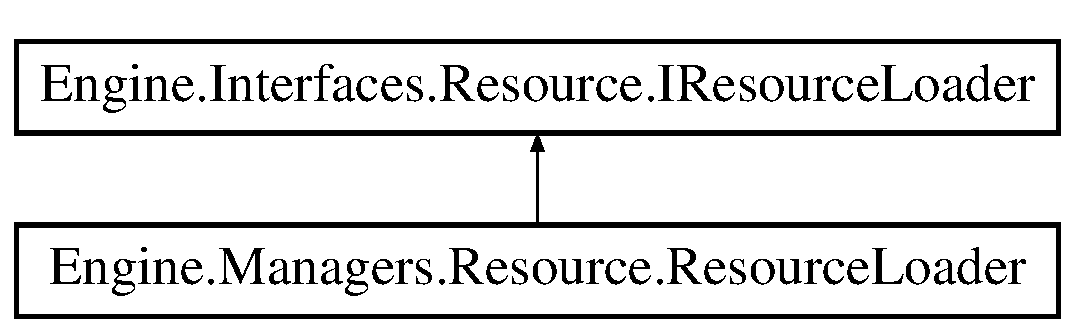
\includegraphics[height=2.000000cm]{da/d7e/a00530}
\end{center}
\end{figure}
\subsection*{Public Member Functions}
\begin{DoxyCompactItemize}
\item 
void \hyperlink{a00530_a77b00bda1dc37c9cabe2dbaf90655714}{Initialize} ()
\begin{DoxyCompactList}\small\item\em M\+E\+T\+H\+OD\+: Initialises and Loads appropriate resources \end{DoxyCompactList}\item 
void \hyperlink{a00530_aa767792c046f7e3e21c512de046dac81}{Load\+Texture} (string path)
\begin{DoxyCompactList}\small\item\em M\+E\+T\+H\+OD\+: Takes a string parameter and attempts to load a texture pointed to from the string. \end{DoxyCompactList}\item 
void \hyperlink{a00530_aed066679a7bd0ff5549d13323c88d4b4}{Load\+Texture} (string start, string name)
\begin{DoxyCompactList}\small\item\em M\+E\+T\+H\+OD\+: Takes two strings, one as the directory, if not the same as the Content pipeline, and one as the file name and attempts to load the texture \end{DoxyCompactList}\item 
Texture2D \hyperlink{a00530_a841de899c3601b3d35496ee798a6e894}{Get\+Tex} (string name)
\begin{DoxyCompactList}\small\item\em M\+E\+T\+H\+OD\+: returns a Texture from the string provided \end{DoxyCompactList}\item 
void \hyperlink{a00530_ab0e1965354b92f0fc2920c74b48a7f0d}{Load\+Font} (string start, string name)
\begin{DoxyCompactList}\small\item\em M\+E\+T\+H\+OD\+: Load a Sprite\+Font from the content pipeline via a string and add it into the dictionary \end{DoxyCompactList}\item 
Sprite\+Font \hyperlink{a00530_a160f06963928da598da9f9431ba65f73}{Get\+Font} (string Name)
\begin{DoxyCompactList}\small\item\em M\+E\+T\+H\+OD\+: Get a font from a string directory \end{DoxyCompactList}\item 
bool \hyperlink{a00530_a939824a1d16e96b4322225a18f7a47d6}{Check\+Library} (string name)
\begin{DoxyCompactList}\small\item\em M\+E\+T\+H\+OD\+: Checks the current song library for an audio file with the name provided in parameters \end{DoxyCompactList}\item 
void \hyperlink{a00530_aa8ac4f03379c9dd95e96ca38b6da344b}{Lo\+Engineong} (string start, string name)
\begin{DoxyCompactList}\small\item\em M\+E\+T\+H\+OD\+: Load a song if it is not already in the queue \end{DoxyCompactList}\item 
Song \hyperlink{a00530_a6587452c5637a132330fb0e2f6dc4e7a}{Get\+Song} (string name)
\begin{DoxyCompactList}\small\item\em M\+E\+T\+H\+OD\+: Return a song based on the string given in parameters \end{DoxyCompactList}\item 
void \hyperlink{a00530_a3c054651a1f23dd6a968336f2079f1b2}{Load\+Tiles} ()
\begin{DoxyCompactList}\small\item\em M\+E\+T\+H\+OD\+: Load the textures for any tiles to be used. \end{DoxyCompactList}\item 
void \hyperlink{a00530_a557cc78880f9acf324eb77d9be245c98}{Lo\+Engineound} ()
\begin{DoxyCompactList}\small\item\em M\+E\+T\+H\+OD\+: Load any sound files to be used \end{DoxyCompactList}\item 
void \hyperlink{a00530_a8ed087cf44b8c303edb0d8b59efb3a9b}{Load\+Entity} ()
\begin{DoxyCompactList}\small\item\em M\+E\+T\+H\+OD\+: Load any entity textures to be used \end{DoxyCompactList}\item 
void \hyperlink{a00530_a19d917cb5f5580c6c4a4fa00c3f63daa}{Load\+Misc} ()
\begin{DoxyCompactList}\small\item\em M\+E\+T\+H\+OD\+: Load any miscellaneous Objects to be used \end{DoxyCompactList}\item 
void \hyperlink{a00530_ab4c5158cd1df0416f5abdc9d82eccf9f}{Load\+G\+UI} ()
\begin{DoxyCompactList}\small\item\em M\+E\+T\+H\+OD\+: Load any G\+UI Assets \end{DoxyCompactList}\end{DoxyCompactItemize}
\subsection*{Data Fields}
\begin{DoxyCompactItemize}
\item 
Dictionary$<$ string, Sprite\+Font $>$ \hyperlink{a00530_a00c311d64cae0ba6d592ea37dafffdc8}{Fonts} = new Dictionary$<$string, Sprite\+Font$>$()
\begin{DoxyCompactList}\small\item\em D\+E\+C\+L\+A\+RE\+: Dictionary for Spritefonts. \end{DoxyCompactList}\item 
Dictionary$<$ string, Texture2D $>$ \hyperlink{a00530_a0a1c5385822e9334a2747b4dac701ec9}{Textures} = new Dictionary$<$string, Texture2D$>$()
\begin{DoxyCompactList}\small\item\em D\+E\+C\+L\+A\+RE\+: Dictionary for the type of Texture2D. \end{DoxyCompactList}\item 
Dictionary$<$ string, Song $>$ \hyperlink{a00530_a2b471bcf803817288914773957bc3e4e}{Music} = new Dictionary$<$string, Song$>$()
\begin{DoxyCompactList}\small\item\em D\+E\+C\+L\+A\+RE\+: Dictionray for the type of Song. \end{DoxyCompactList}\end{DoxyCompactItemize}
\subsection*{Properties}
\begin{DoxyCompactItemize}
\item 
Content\+Manager \hyperlink{a00530_a4d635d8ea6e09eb1e403da947ac92bc2}{Content}\hspace{0.3cm}{\ttfamily  \mbox{[}get, set\mbox{]}}
\begin{DoxyCompactList}\small\item\em G\+ET\+: S\+ET\+: Monogame Content\+Manager. \end{DoxyCompactList}\end{DoxyCompactItemize}


\subsection{Detailed Description}
C\+L\+A\+SS\+: The \hyperlink{a00272}{Resource} loader is responsible for loading and storage of external resources such as textures and sounds 



\subsection{Member Function Documentation}
\mbox{\Hypertarget{a00530_a939824a1d16e96b4322225a18f7a47d6}\label{a00530_a939824a1d16e96b4322225a18f7a47d6}} 
\index{Engine\+::\+Managers\+::\+Resource\+::\+Resource\+Loader@{Engine\+::\+Managers\+::\+Resource\+::\+Resource\+Loader}!Check\+Library@{Check\+Library}}
\index{Check\+Library@{Check\+Library}!Engine\+::\+Managers\+::\+Resource\+::\+Resource\+Loader@{Engine\+::\+Managers\+::\+Resource\+::\+Resource\+Loader}}
\subsubsection{\texorpdfstring{Check\+Library()}{CheckLibrary()}}
{\footnotesize\ttfamily bool Engine.\+Managers.\+Resource.\+Resource\+Loader.\+Check\+Library (\begin{DoxyParamCaption}\item[{string}]{name }\end{DoxyParamCaption})\hspace{0.3cm}{\ttfamily [inline]}}



M\+E\+T\+H\+OD\+: Checks the current song library for an audio file with the name provided in parameters 


\begin{DoxyParams}{Parameters}
{\em name} & The name of the audio file requested\\
\hline
\end{DoxyParams}
\begin{DoxyReturn}{Returns}
a boolean for if the audio file is in the library or queue
\end{DoxyReturn}


Implements \hyperlink{a00462_a08d51ffa3d65fd1122614e00a275cf48}{Engine.\+Interfaces.\+Resource.\+I\+Resource\+Loader}.

\mbox{\Hypertarget{a00530_a160f06963928da598da9f9431ba65f73}\label{a00530_a160f06963928da598da9f9431ba65f73}} 
\index{Engine\+::\+Managers\+::\+Resource\+::\+Resource\+Loader@{Engine\+::\+Managers\+::\+Resource\+::\+Resource\+Loader}!Get\+Font@{Get\+Font}}
\index{Get\+Font@{Get\+Font}!Engine\+::\+Managers\+::\+Resource\+::\+Resource\+Loader@{Engine\+::\+Managers\+::\+Resource\+::\+Resource\+Loader}}
\subsubsection{\texorpdfstring{Get\+Font()}{GetFont()}}
{\footnotesize\ttfamily Sprite\+Font Engine.\+Managers.\+Resource.\+Resource\+Loader.\+Get\+Font (\begin{DoxyParamCaption}\item[{string}]{name }\end{DoxyParamCaption})\hspace{0.3cm}{\ttfamily [inline]}}



M\+E\+T\+H\+OD\+: Get a font from a string directory 


\begin{DoxyParams}{Parameters}
{\em name} & The name of the font file to be loaded\\
\hline
\end{DoxyParams}
\begin{DoxyReturn}{Returns}
a Sprite\+Font of the font at the name provided
\end{DoxyReturn}


Implements \hyperlink{a00462_abe9339a97b29bce2ba8a77504495f27d}{Engine.\+Interfaces.\+Resource.\+I\+Resource\+Loader}.

\mbox{\Hypertarget{a00530_a6587452c5637a132330fb0e2f6dc4e7a}\label{a00530_a6587452c5637a132330fb0e2f6dc4e7a}} 
\index{Engine\+::\+Managers\+::\+Resource\+::\+Resource\+Loader@{Engine\+::\+Managers\+::\+Resource\+::\+Resource\+Loader}!Get\+Song@{Get\+Song}}
\index{Get\+Song@{Get\+Song}!Engine\+::\+Managers\+::\+Resource\+::\+Resource\+Loader@{Engine\+::\+Managers\+::\+Resource\+::\+Resource\+Loader}}
\subsubsection{\texorpdfstring{Get\+Song()}{GetSong()}}
{\footnotesize\ttfamily Song Engine.\+Managers.\+Resource.\+Resource\+Loader.\+Get\+Song (\begin{DoxyParamCaption}\item[{string}]{name }\end{DoxyParamCaption})\hspace{0.3cm}{\ttfamily [inline]}}



M\+E\+T\+H\+OD\+: Return a song based on the string given in parameters 


\begin{DoxyParams}{Parameters}
{\em name} & The name of the file to be searched for in the music library\\
\hline
\end{DoxyParams}
\begin{DoxyReturn}{Returns}
A song of the same name
\end{DoxyReturn}


Implements \hyperlink{a00462_a6d962a64dc4f377bdb417598b17c53d0}{Engine.\+Interfaces.\+Resource.\+I\+Resource\+Loader}.

\mbox{\Hypertarget{a00530_a841de899c3601b3d35496ee798a6e894}\label{a00530_a841de899c3601b3d35496ee798a6e894}} 
\index{Engine\+::\+Managers\+::\+Resource\+::\+Resource\+Loader@{Engine\+::\+Managers\+::\+Resource\+::\+Resource\+Loader}!Get\+Tex@{Get\+Tex}}
\index{Get\+Tex@{Get\+Tex}!Engine\+::\+Managers\+::\+Resource\+::\+Resource\+Loader@{Engine\+::\+Managers\+::\+Resource\+::\+Resource\+Loader}}
\subsubsection{\texorpdfstring{Get\+Tex()}{GetTex()}}
{\footnotesize\ttfamily Texture2D Engine.\+Managers.\+Resource.\+Resource\+Loader.\+Get\+Tex (\begin{DoxyParamCaption}\item[{string}]{name }\end{DoxyParamCaption})\hspace{0.3cm}{\ttfamily [inline]}}



M\+E\+T\+H\+OD\+: returns a Texture from the string provided 


\begin{DoxyParams}{Parameters}
{\em name} & The name of the file\\
\hline
\end{DoxyParams}
\begin{DoxyReturn}{Returns}
A texture2D of the same name
\end{DoxyReturn}


Implements \hyperlink{a00462_ad126b831364ad6219c3f25729c591597}{Engine.\+Interfaces.\+Resource.\+I\+Resource\+Loader}.

\mbox{\Hypertarget{a00530_a77b00bda1dc37c9cabe2dbaf90655714}\label{a00530_a77b00bda1dc37c9cabe2dbaf90655714}} 
\index{Engine\+::\+Managers\+::\+Resource\+::\+Resource\+Loader@{Engine\+::\+Managers\+::\+Resource\+::\+Resource\+Loader}!Initialize@{Initialize}}
\index{Initialize@{Initialize}!Engine\+::\+Managers\+::\+Resource\+::\+Resource\+Loader@{Engine\+::\+Managers\+::\+Resource\+::\+Resource\+Loader}}
\subsubsection{\texorpdfstring{Initialize()}{Initialize()}}
{\footnotesize\ttfamily void Engine.\+Managers.\+Resource.\+Resource\+Loader.\+Initialize (\begin{DoxyParamCaption}{ }\end{DoxyParamCaption})\hspace{0.3cm}{\ttfamily [inline]}}



M\+E\+T\+H\+OD\+: Initialises and Loads appropriate resources 



Implements \hyperlink{a00462_ad861af436f861ea7d9c0966edfadac82}{Engine.\+Interfaces.\+Resource.\+I\+Resource\+Loader}.

\mbox{\Hypertarget{a00530_a8ed087cf44b8c303edb0d8b59efb3a9b}\label{a00530_a8ed087cf44b8c303edb0d8b59efb3a9b}} 
\index{Engine\+::\+Managers\+::\+Resource\+::\+Resource\+Loader@{Engine\+::\+Managers\+::\+Resource\+::\+Resource\+Loader}!Load\+Entity@{Load\+Entity}}
\index{Load\+Entity@{Load\+Entity}!Engine\+::\+Managers\+::\+Resource\+::\+Resource\+Loader@{Engine\+::\+Managers\+::\+Resource\+::\+Resource\+Loader}}
\subsubsection{\texorpdfstring{Load\+Entity()}{LoadEntity()}}
{\footnotesize\ttfamily void Engine.\+Managers.\+Resource.\+Resource\+Loader.\+Load\+Entity (\begin{DoxyParamCaption}{ }\end{DoxyParamCaption})\hspace{0.3cm}{\ttfamily [inline]}}



M\+E\+T\+H\+OD\+: Load any entity textures to be used 

\mbox{\Hypertarget{a00530_ab0e1965354b92f0fc2920c74b48a7f0d}\label{a00530_ab0e1965354b92f0fc2920c74b48a7f0d}} 
\index{Engine\+::\+Managers\+::\+Resource\+::\+Resource\+Loader@{Engine\+::\+Managers\+::\+Resource\+::\+Resource\+Loader}!Load\+Font@{Load\+Font}}
\index{Load\+Font@{Load\+Font}!Engine\+::\+Managers\+::\+Resource\+::\+Resource\+Loader@{Engine\+::\+Managers\+::\+Resource\+::\+Resource\+Loader}}
\subsubsection{\texorpdfstring{Load\+Font()}{LoadFont()}}
{\footnotesize\ttfamily void Engine.\+Managers.\+Resource.\+Resource\+Loader.\+Load\+Font (\begin{DoxyParamCaption}\item[{string}]{start,  }\item[{string}]{name }\end{DoxyParamCaption})\hspace{0.3cm}{\ttfamily [inline]}}



M\+E\+T\+H\+OD\+: Load a Sprite\+Font from the content pipeline via a string and add it into the dictionary 


\begin{DoxyParams}{Parameters}
{\em start} & The folder of the file\\
\hline
{\em name} & The name of the file\\
\hline
\end{DoxyParams}
\mbox{\Hypertarget{a00530_ab4c5158cd1df0416f5abdc9d82eccf9f}\label{a00530_ab4c5158cd1df0416f5abdc9d82eccf9f}} 
\index{Engine\+::\+Managers\+::\+Resource\+::\+Resource\+Loader@{Engine\+::\+Managers\+::\+Resource\+::\+Resource\+Loader}!Load\+G\+UI@{Load\+G\+UI}}
\index{Load\+G\+UI@{Load\+G\+UI}!Engine\+::\+Managers\+::\+Resource\+::\+Resource\+Loader@{Engine\+::\+Managers\+::\+Resource\+::\+Resource\+Loader}}
\subsubsection{\texorpdfstring{Load\+G\+U\+I()}{LoadGUI()}}
{\footnotesize\ttfamily void Engine.\+Managers.\+Resource.\+Resource\+Loader.\+Load\+G\+UI (\begin{DoxyParamCaption}{ }\end{DoxyParamCaption})\hspace{0.3cm}{\ttfamily [inline]}}



M\+E\+T\+H\+OD\+: Load any G\+UI Assets 

\mbox{\Hypertarget{a00530_a19d917cb5f5580c6c4a4fa00c3f63daa}\label{a00530_a19d917cb5f5580c6c4a4fa00c3f63daa}} 
\index{Engine\+::\+Managers\+::\+Resource\+::\+Resource\+Loader@{Engine\+::\+Managers\+::\+Resource\+::\+Resource\+Loader}!Load\+Misc@{Load\+Misc}}
\index{Load\+Misc@{Load\+Misc}!Engine\+::\+Managers\+::\+Resource\+::\+Resource\+Loader@{Engine\+::\+Managers\+::\+Resource\+::\+Resource\+Loader}}
\subsubsection{\texorpdfstring{Load\+Misc()}{LoadMisc()}}
{\footnotesize\ttfamily void Engine.\+Managers.\+Resource.\+Resource\+Loader.\+Load\+Misc (\begin{DoxyParamCaption}{ }\end{DoxyParamCaption})\hspace{0.3cm}{\ttfamily [inline]}}



M\+E\+T\+H\+OD\+: Load any miscellaneous Objects to be used 

\mbox{\Hypertarget{a00530_aa767792c046f7e3e21c512de046dac81}\label{a00530_aa767792c046f7e3e21c512de046dac81}} 
\index{Engine\+::\+Managers\+::\+Resource\+::\+Resource\+Loader@{Engine\+::\+Managers\+::\+Resource\+::\+Resource\+Loader}!Load\+Texture@{Load\+Texture}}
\index{Load\+Texture@{Load\+Texture}!Engine\+::\+Managers\+::\+Resource\+::\+Resource\+Loader@{Engine\+::\+Managers\+::\+Resource\+::\+Resource\+Loader}}
\subsubsection{\texorpdfstring{Load\+Texture()}{LoadTexture()}\hspace{0.1cm}{\footnotesize\ttfamily [1/2]}}
{\footnotesize\ttfamily void Engine.\+Managers.\+Resource.\+Resource\+Loader.\+Load\+Texture (\begin{DoxyParamCaption}\item[{string}]{path }\end{DoxyParamCaption})\hspace{0.3cm}{\ttfamily [inline]}}



M\+E\+T\+H\+OD\+: Takes a string parameter and attempts to load a texture pointed to from the string. 


\begin{DoxyParams}{Parameters}
{\em path} & The path of the texture to be loaded\\
\hline
\end{DoxyParams}
\mbox{\Hypertarget{a00530_aed066679a7bd0ff5549d13323c88d4b4}\label{a00530_aed066679a7bd0ff5549d13323c88d4b4}} 
\index{Engine\+::\+Managers\+::\+Resource\+::\+Resource\+Loader@{Engine\+::\+Managers\+::\+Resource\+::\+Resource\+Loader}!Load\+Texture@{Load\+Texture}}
\index{Load\+Texture@{Load\+Texture}!Engine\+::\+Managers\+::\+Resource\+::\+Resource\+Loader@{Engine\+::\+Managers\+::\+Resource\+::\+Resource\+Loader}}
\subsubsection{\texorpdfstring{Load\+Texture()}{LoadTexture()}\hspace{0.1cm}{\footnotesize\ttfamily [2/2]}}
{\footnotesize\ttfamily void Engine.\+Managers.\+Resource.\+Resource\+Loader.\+Load\+Texture (\begin{DoxyParamCaption}\item[{string}]{start,  }\item[{string}]{name }\end{DoxyParamCaption})\hspace{0.3cm}{\ttfamily [inline]}}



M\+E\+T\+H\+OD\+: Takes two strings, one as the directory, if not the same as the Content pipeline, and one as the file name and attempts to load the texture 


\begin{DoxyParams}{Parameters}
{\em start} & The folder of the file\\
\hline
{\em name} & The name of the file\\
\hline
\end{DoxyParams}
\mbox{\Hypertarget{a00530_a3c054651a1f23dd6a968336f2079f1b2}\label{a00530_a3c054651a1f23dd6a968336f2079f1b2}} 
\index{Engine\+::\+Managers\+::\+Resource\+::\+Resource\+Loader@{Engine\+::\+Managers\+::\+Resource\+::\+Resource\+Loader}!Load\+Tiles@{Load\+Tiles}}
\index{Load\+Tiles@{Load\+Tiles}!Engine\+::\+Managers\+::\+Resource\+::\+Resource\+Loader@{Engine\+::\+Managers\+::\+Resource\+::\+Resource\+Loader}}
\subsubsection{\texorpdfstring{Load\+Tiles()}{LoadTiles()}}
{\footnotesize\ttfamily void Engine.\+Managers.\+Resource.\+Resource\+Loader.\+Load\+Tiles (\begin{DoxyParamCaption}{ }\end{DoxyParamCaption})\hspace{0.3cm}{\ttfamily [inline]}}



M\+E\+T\+H\+OD\+: Load the textures for any tiles to be used. 

\mbox{\Hypertarget{a00530_aa8ac4f03379c9dd95e96ca38b6da344b}\label{a00530_aa8ac4f03379c9dd95e96ca38b6da344b}} 
\index{Engine\+::\+Managers\+::\+Resource\+::\+Resource\+Loader@{Engine\+::\+Managers\+::\+Resource\+::\+Resource\+Loader}!Lo\+Engineong@{Lo\+Engineong}}
\index{Lo\+Engineong@{Lo\+Engineong}!Engine\+::\+Managers\+::\+Resource\+::\+Resource\+Loader@{Engine\+::\+Managers\+::\+Resource\+::\+Resource\+Loader}}
\subsubsection{\texorpdfstring{Lo\+Engineong()}{LoEngineong()}}
{\footnotesize\ttfamily void Engine.\+Managers.\+Resource.\+Resource\+Loader.\+Lo\+Engineong (\begin{DoxyParamCaption}\item[{string}]{start,  }\item[{string}]{name }\end{DoxyParamCaption})\hspace{0.3cm}{\ttfamily [inline]}}



M\+E\+T\+H\+OD\+: Load a song if it is not already in the queue 


\begin{DoxyParams}{Parameters}
{\em start} & the folder of the song\\
\hline
{\em name} & the name of the song\\
\hline
\end{DoxyParams}
\mbox{\Hypertarget{a00530_a557cc78880f9acf324eb77d9be245c98}\label{a00530_a557cc78880f9acf324eb77d9be245c98}} 
\index{Engine\+::\+Managers\+::\+Resource\+::\+Resource\+Loader@{Engine\+::\+Managers\+::\+Resource\+::\+Resource\+Loader}!Lo\+Engineound@{Lo\+Engineound}}
\index{Lo\+Engineound@{Lo\+Engineound}!Engine\+::\+Managers\+::\+Resource\+::\+Resource\+Loader@{Engine\+::\+Managers\+::\+Resource\+::\+Resource\+Loader}}
\subsubsection{\texorpdfstring{Lo\+Engineound()}{LoEngineound()}}
{\footnotesize\ttfamily void Engine.\+Managers.\+Resource.\+Resource\+Loader.\+Lo\+Engineound (\begin{DoxyParamCaption}{ }\end{DoxyParamCaption})\hspace{0.3cm}{\ttfamily [inline]}}



M\+E\+T\+H\+OD\+: Load any sound files to be used 



\subsection{Field Documentation}
\mbox{\Hypertarget{a00530_a00c311d64cae0ba6d592ea37dafffdc8}\label{a00530_a00c311d64cae0ba6d592ea37dafffdc8}} 
\index{Engine\+::\+Managers\+::\+Resource\+::\+Resource\+Loader@{Engine\+::\+Managers\+::\+Resource\+::\+Resource\+Loader}!Fonts@{Fonts}}
\index{Fonts@{Fonts}!Engine\+::\+Managers\+::\+Resource\+::\+Resource\+Loader@{Engine\+::\+Managers\+::\+Resource\+::\+Resource\+Loader}}
\subsubsection{\texorpdfstring{Fonts}{Fonts}}
{\footnotesize\ttfamily Dictionary$<$string, Sprite\+Font$>$ Engine.\+Managers.\+Resource.\+Resource\+Loader.\+Fonts = new Dictionary$<$string, Sprite\+Font$>$()}



D\+E\+C\+L\+A\+RE\+: Dictionary for Spritefonts. 

\mbox{\Hypertarget{a00530_a2b471bcf803817288914773957bc3e4e}\label{a00530_a2b471bcf803817288914773957bc3e4e}} 
\index{Engine\+::\+Managers\+::\+Resource\+::\+Resource\+Loader@{Engine\+::\+Managers\+::\+Resource\+::\+Resource\+Loader}!Music@{Music}}
\index{Music@{Music}!Engine\+::\+Managers\+::\+Resource\+::\+Resource\+Loader@{Engine\+::\+Managers\+::\+Resource\+::\+Resource\+Loader}}
\subsubsection{\texorpdfstring{Music}{Music}}
{\footnotesize\ttfamily Dictionary$<$string, Song$>$ Engine.\+Managers.\+Resource.\+Resource\+Loader.\+Music = new Dictionary$<$string, Song$>$()}



D\+E\+C\+L\+A\+RE\+: Dictionray for the type of Song. 

\mbox{\Hypertarget{a00530_a0a1c5385822e9334a2747b4dac701ec9}\label{a00530_a0a1c5385822e9334a2747b4dac701ec9}} 
\index{Engine\+::\+Managers\+::\+Resource\+::\+Resource\+Loader@{Engine\+::\+Managers\+::\+Resource\+::\+Resource\+Loader}!Textures@{Textures}}
\index{Textures@{Textures}!Engine\+::\+Managers\+::\+Resource\+::\+Resource\+Loader@{Engine\+::\+Managers\+::\+Resource\+::\+Resource\+Loader}}
\subsubsection{\texorpdfstring{Textures}{Textures}}
{\footnotesize\ttfamily Dictionary$<$string, Texture2D$>$ Engine.\+Managers.\+Resource.\+Resource\+Loader.\+Textures = new Dictionary$<$string, Texture2D$>$()}



D\+E\+C\+L\+A\+RE\+: Dictionary for the type of Texture2D. 



\subsection{Property Documentation}
\mbox{\Hypertarget{a00530_a4d635d8ea6e09eb1e403da947ac92bc2}\label{a00530_a4d635d8ea6e09eb1e403da947ac92bc2}} 
\index{Engine\+::\+Managers\+::\+Resource\+::\+Resource\+Loader@{Engine\+::\+Managers\+::\+Resource\+::\+Resource\+Loader}!Content@{Content}}
\index{Content@{Content}!Engine\+::\+Managers\+::\+Resource\+::\+Resource\+Loader@{Engine\+::\+Managers\+::\+Resource\+::\+Resource\+Loader}}
\subsubsection{\texorpdfstring{Content}{Content}}
{\footnotesize\ttfamily Content\+Manager Engine.\+Managers.\+Resource.\+Resource\+Loader.\+Content\hspace{0.3cm}{\ttfamily [get]}, {\ttfamily [set]}}



G\+ET\+: S\+ET\+: Monogame Content\+Manager. 



The documentation for this class was generated from the following file\+:\begin{DoxyCompactItemize}
\item 
\hyperlink{a00179}{Resource\+Loader.\+cs}\end{DoxyCompactItemize}

\hypertarget{a00510}{}\section{Engine.\+Managers.\+Collision.\+S\+A\+Tcheck Class Reference}
\label{a00510}\index{Engine.\+Managers.\+Collision.\+S\+A\+Tcheck@{Engine.\+Managers.\+Collision.\+S\+A\+Tcheck}}


C\+L\+A\+SS\+: This class runs all of the Separating Axis Theorem collision code. It calculates whether two shapes are currently intersecting or going to intersect by projecting shadows of both shapes onto an arbitrary axis perpendicular to the edges of the shape.  


\subsection*{Public Member Functions}
\begin{DoxyCompactItemize}
\item 
bool \hyperlink{a00510_a466b04bf6d509f7a713b7aec38391e51}{S\+A\+T\+Collision} (\hyperlink{a00434}{I\+Hitbox} shape1, \hyperlink{a00434}{I\+Hitbox} shape2, Vector2 velocity, Vector2 velocity2)
\begin{DoxyCompactList}\small\item\em M\+E\+T\+H\+OD\+: The calculation for if two objects are colliding or going to collide \end{DoxyCompactList}\item 
void \hyperlink{a00510_a566a1183f83e123c710bd3cc1d240aef}{Projection} (Vector2 axis, \hyperlink{a00434}{I\+Hitbox} my\+Ent, ref float min, ref float max)
\begin{DoxyCompactList}\small\item\em M\+E\+T\+H\+OD\+: Projects an Object onto an arbitrary axis \end{DoxyCompactList}\item 
float \hyperlink{a00510_a5e692998d63a129d3fed2163bcbf8a55}{Interval\+Distance} (float minA, float maxA, float minB, float maxB)
\begin{DoxyCompactList}\small\item\em M\+E\+T\+H\+OD\+: Finds the distance between two values \end{DoxyCompactList}\item 
Vector2 \hyperlink{a00510_a4aa620a587dc54dd480fd0a9fd29d817}{mtv\+Ret} ()
\begin{DoxyCompactList}\small\item\em M\+E\+T\+H\+OD\+: returns the minimum distance needed to move an object to prevent them from being in a collision \end{DoxyCompactList}\end{DoxyCompactItemize}
\subsection*{Data Fields}
\begin{DoxyCompactItemize}
\item 
Vector2 \hyperlink{a00510_a307c7f32a47949b280ac2a9d7b174899}{Minimum\+Translation\+Vector}
\end{DoxyCompactItemize}


\subsection{Detailed Description}
C\+L\+A\+SS\+: This class runs all of the Separating Axis Theorem collision code. It calculates whether two shapes are currently intersecting or going to intersect by projecting shadows of both shapes onto an arbitrary axis perpendicular to the edges of the shape. 



\subsection{Member Function Documentation}
\mbox{\Hypertarget{a00510_a5e692998d63a129d3fed2163bcbf8a55}\label{a00510_a5e692998d63a129d3fed2163bcbf8a55}} 
\index{Engine\+::\+Managers\+::\+Collision\+::\+S\+A\+Tcheck@{Engine\+::\+Managers\+::\+Collision\+::\+S\+A\+Tcheck}!Interval\+Distance@{Interval\+Distance}}
\index{Interval\+Distance@{Interval\+Distance}!Engine\+::\+Managers\+::\+Collision\+::\+S\+A\+Tcheck@{Engine\+::\+Managers\+::\+Collision\+::\+S\+A\+Tcheck}}
\subsubsection{\texorpdfstring{Interval\+Distance()}{IntervalDistance()}}
{\footnotesize\ttfamily float Engine.\+Managers.\+Collision.\+S\+A\+Tcheck.\+Interval\+Distance (\begin{DoxyParamCaption}\item[{float}]{minA,  }\item[{float}]{maxA,  }\item[{float}]{minB,  }\item[{float}]{maxB }\end{DoxyParamCaption})\hspace{0.3cm}{\ttfamily [inline]}}



M\+E\+T\+H\+OD\+: Finds the distance between two values 


\begin{DoxyParams}{Parameters}
{\em minA} & the minimum value of the first object on an axis\\
\hline
{\em maxA} & The maximum value of the first object on an axis\\
\hline
{\em minB} & The minimum value of the second object on an axis\\
\hline
{\em maxB} & The maximum value of the second object on an axis\\
\hline
\end{DoxyParams}
\begin{DoxyReturn}{Returns}
A float of the distance between two values
\end{DoxyReturn}
whichever is lower on the axis

Return the one on the right minus the other

Return the one on the right minus the other \mbox{\Hypertarget{a00510_a4aa620a587dc54dd480fd0a9fd29d817}\label{a00510_a4aa620a587dc54dd480fd0a9fd29d817}} 
\index{Engine\+::\+Managers\+::\+Collision\+::\+S\+A\+Tcheck@{Engine\+::\+Managers\+::\+Collision\+::\+S\+A\+Tcheck}!mtv\+Ret@{mtv\+Ret}}
\index{mtv\+Ret@{mtv\+Ret}!Engine\+::\+Managers\+::\+Collision\+::\+S\+A\+Tcheck@{Engine\+::\+Managers\+::\+Collision\+::\+S\+A\+Tcheck}}
\subsubsection{\texorpdfstring{mtv\+Ret()}{mtvRet()}}
{\footnotesize\ttfamily Vector2 Engine.\+Managers.\+Collision.\+S\+A\+Tcheck.\+mtv\+Ret (\begin{DoxyParamCaption}{ }\end{DoxyParamCaption})\hspace{0.3cm}{\ttfamily [inline]}}



M\+E\+T\+H\+OD\+: returns the minimum distance needed to move an object to prevent them from being in a collision 

\begin{DoxyReturn}{Returns}
A vector2 Of the minimum translation vector
\end{DoxyReturn}
Return the minimum distance required to prevent shapes from intersecting \mbox{\Hypertarget{a00510_a566a1183f83e123c710bd3cc1d240aef}\label{a00510_a566a1183f83e123c710bd3cc1d240aef}} 
\index{Engine\+::\+Managers\+::\+Collision\+::\+S\+A\+Tcheck@{Engine\+::\+Managers\+::\+Collision\+::\+S\+A\+Tcheck}!Projection@{Projection}}
\index{Projection@{Projection}!Engine\+::\+Managers\+::\+Collision\+::\+S\+A\+Tcheck@{Engine\+::\+Managers\+::\+Collision\+::\+S\+A\+Tcheck}}
\subsubsection{\texorpdfstring{Projection()}{Projection()}}
{\footnotesize\ttfamily void Engine.\+Managers.\+Collision.\+S\+A\+Tcheck.\+Projection (\begin{DoxyParamCaption}\item[{Vector2}]{axis,  }\item[{\hyperlink{a00434}{I\+Hitbox}}]{my\+Ent,  }\item[{ref float}]{min,  }\item[{ref float}]{max }\end{DoxyParamCaption})\hspace{0.3cm}{\ttfamily [inline]}}



M\+E\+T\+H\+OD\+: Projects an Object onto an arbitrary axis 


\begin{DoxyParams}{Parameters}
{\em axis} & The axis to be projected on to\\
\hline
{\em my\+Ent} & The object to be projected\\
\hline
{\em min} & The minimum value of the object on the axis\\
\hline
{\em max} & The maximum value of the object on the axis\\
\hline
\end{DoxyParams}
To project a point on an axis use the dot product

Find the minimum point along the axis that the shape can be found. Set the min and max accordingly \mbox{\Hypertarget{a00510_a466b04bf6d509f7a713b7aec38391e51}\label{a00510_a466b04bf6d509f7a713b7aec38391e51}} 
\index{Engine\+::\+Managers\+::\+Collision\+::\+S\+A\+Tcheck@{Engine\+::\+Managers\+::\+Collision\+::\+S\+A\+Tcheck}!S\+A\+T\+Collision@{S\+A\+T\+Collision}}
\index{S\+A\+T\+Collision@{S\+A\+T\+Collision}!Engine\+::\+Managers\+::\+Collision\+::\+S\+A\+Tcheck@{Engine\+::\+Managers\+::\+Collision\+::\+S\+A\+Tcheck}}
\subsubsection{\texorpdfstring{S\+A\+T\+Collision()}{SATCollision()}}
{\footnotesize\ttfamily bool Engine.\+Managers.\+Collision.\+S\+A\+Tcheck.\+S\+A\+T\+Collision (\begin{DoxyParamCaption}\item[{\hyperlink{a00434}{I\+Hitbox}}]{shape1,  }\item[{\hyperlink{a00434}{I\+Hitbox}}]{shape2,  }\item[{Vector2}]{velocity,  }\item[{Vector2}]{velocity2 }\end{DoxyParamCaption})\hspace{0.3cm}{\ttfamily [inline]}}



M\+E\+T\+H\+OD\+: The calculation for if two objects are colliding or going to collide 


\begin{DoxyParams}{Parameters}
{\em shape1} & The first object in the calculation\\
\hline
{\em shape2} & The second object in the calculation\\
\hline
{\em velocity} & The velocity of the first object\\
\hline
{\em velocity2} & The velocity of the second object\\
\hline
\end{DoxyParams}
\begin{DoxyReturn}{Returns}
A bool of whether the shapes are about to collide or are already colliding
\end{DoxyReturn}
assume the shape is intersecting until calculated

Assume the shape will intersect until calculated

C\+R\+E\+A\+TE\+: an integer of how many edges are in shape 1

C\+R\+E\+A\+TE\+: an integer of how many edges are in shape 2

S\+ET\+: Minimum translation vector is set to infinity

I\+N\+I\+T\+I\+A\+L\+I\+SE\+: The axis that we will push the shape along if its colliding

D\+E\+C\+L\+A\+RE\+: The current edge we are checking

F\+OR\+: all the edges of both polygons

IF e is less than the first integer, we are checking each edge of the first shape

Same for shape 2

S\+ET\+: the axis perpendicular to the current edge to project on

Keeping the vector pointing the same direction, adjust it so it\textquotesingle{}s length is 1

S\+ET\+: the projection of the polygon on the current axis

These are initialised to 0 and adjusted in the method below

Project polygon onto axis

Project polygon 2 onto axis

IF\+: the polygon projections are currently N\+OT intersecting

This if statement will only run if the first condition of the method is met, therefore we know they aren\textquotesingle{}t intersecting

S\+ET\+: the velocity projection on the current axis by using the dot product.

IF\+: the Projection of polygon A is less than 0

S\+ET\+: The Min variable accordingly.

E\+L\+SE S\+ET\+: the max variable accordingly

Do the same test as above for the new projection

Same as above but this time using a hypothetical movement

IF\+: the polygons are not intersecting and won\textquotesingle{}t intersect, exit the loop

Check if the current interval distance is the minimum one. If so store the interval distance and the current distance. This will be used to calculate the minimum translation vector

Find how far from 0 the distance is

If the minimum translation vector is not the smallest possible movement

Set the vector to the smallest distance!

We need to move the object on the axis we projected

We need to find which object is on the left hand side of the other

The minimum translation vector can be used to push the polygons apart.

If the objects are colliding

Set the property to be the translation axis multiplied by the mtv 

\subsection{Field Documentation}
\mbox{\Hypertarget{a00510_a307c7f32a47949b280ac2a9d7b174899}\label{a00510_a307c7f32a47949b280ac2a9d7b174899}} 
\index{Engine\+::\+Managers\+::\+Collision\+::\+S\+A\+Tcheck@{Engine\+::\+Managers\+::\+Collision\+::\+S\+A\+Tcheck}!Minimum\+Translation\+Vector@{Minimum\+Translation\+Vector}}
\index{Minimum\+Translation\+Vector@{Minimum\+Translation\+Vector}!Engine\+::\+Managers\+::\+Collision\+::\+S\+A\+Tcheck@{Engine\+::\+Managers\+::\+Collision\+::\+S\+A\+Tcheck}}
\subsubsection{\texorpdfstring{Minimum\+Translation\+Vector}{MinimumTranslationVector}}
{\footnotesize\ttfamily Vector2 Engine.\+Managers.\+Collision.\+S\+A\+Tcheck.\+Minimum\+Translation\+Vector}



The documentation for this class was generated from the following file\+:\begin{DoxyCompactItemize}
\item 
\hyperlink{a00164}{S\+A\+Tcheck.\+cs}\end{DoxyCompactItemize}

\hypertarget{a00566}{}\section{Engine.\+S\+A\+T\+Demo Class Reference}
\label{a00566}\index{Engine.\+S\+A\+T\+Demo@{Engine.\+S\+A\+T\+Demo}}


C\+L\+A\+SS\+: This class is used for demonstrating the Separating Axis Theorem Collision Behaviour  


Inheritance diagram for Engine.\+S\+A\+T\+Demo\+:\begin{figure}[H]
\begin{center}
\leavevmode
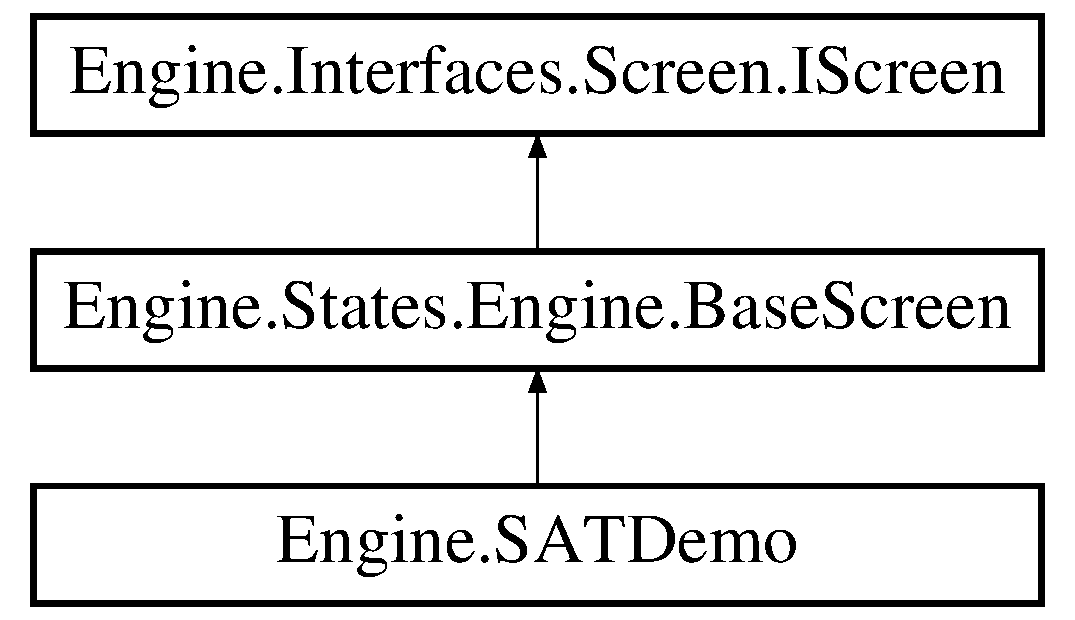
\includegraphics[height=3.000000cm]{d0/d3e/a00566}
\end{center}
\end{figure}
\subsection*{Public Member Functions}
\begin{DoxyCompactItemize}
\item 
override void \hyperlink{a00566_a051d8aea070a4c7a93f0cf494e4fac6a}{Initialize} ()
\begin{DoxyCompactList}\small\item\em M\+E\+T\+H\+OD\+: Initialisation Logic in here \end{DoxyCompactList}\end{DoxyCompactItemize}
\subsection*{Additional Inherited Members}


\subsection{Detailed Description}
C\+L\+A\+SS\+: This class is used for demonstrating the Separating Axis Theorem Collision Behaviour 



\subsection{Member Function Documentation}
\mbox{\Hypertarget{a00566_a051d8aea070a4c7a93f0cf494e4fac6a}\label{a00566_a051d8aea070a4c7a93f0cf494e4fac6a}} 
\index{Engine\+::\+S\+A\+T\+Demo@{Engine\+::\+S\+A\+T\+Demo}!Initialize@{Initialize}}
\index{Initialize@{Initialize}!Engine\+::\+S\+A\+T\+Demo@{Engine\+::\+S\+A\+T\+Demo}}
\subsubsection{\texorpdfstring{Initialize()}{Initialize()}}
{\footnotesize\ttfamily override void Engine.\+S\+A\+T\+Demo.\+Initialize (\begin{DoxyParamCaption}{ }\end{DoxyParamCaption})\hspace{0.3cm}{\ttfamily [inline]}, {\ttfamily [virtual]}}



M\+E\+T\+H\+OD\+: Initialisation Logic in here 

A\+DD\+: entities for testing the collision 

Reimplemented from \hyperlink{a00550_af8fd6890abf865641e190578ef2e054c}{Engine.\+States.\+Engine.\+Base\+Screen}.



The documentation for this class was generated from the following file\+:\begin{DoxyCompactItemize}
\item 
\hyperlink{a00206}{S\+A\+T\+Demo.\+cs}\end{DoxyCompactItemize}

\hypertarget{a00358}{}\section{Engine.\+Events.\+Collision\+Event.\+S\+A\+T\+Event\+Args Class Reference}
\label{a00358}\index{Engine.\+Events.\+Collision\+Event.\+S\+A\+T\+Event\+Args@{Engine.\+Events.\+Collision\+Event.\+S\+A\+T\+Event\+Args}}
\subsection*{Properties}
\begin{DoxyCompactItemize}
\item 
\hyperlink{a00426}{I\+Collidable} \hyperlink{a00358_a89209485aa9a603c076827189dde27d2}{A}\hspace{0.3cm}{\ttfamily  \mbox{[}get, set\mbox{]}}
\item 
\hyperlink{a00426}{I\+Collidable} \hyperlink{a00358_aa3c39db7372b8a976886c9b99870cda9}{B}\hspace{0.3cm}{\ttfamily  \mbox{[}get, set\mbox{]}}
\item 
Vector2 \hyperlink{a00358_a85c32987b6db7fcef61f441e045b9ade}{mtv\+Ret}\hspace{0.3cm}{\ttfamily  \mbox{[}get, set\mbox{]}}
\end{DoxyCompactItemize}


\subsection{Property Documentation}
\mbox{\Hypertarget{a00358_a89209485aa9a603c076827189dde27d2}\label{a00358_a89209485aa9a603c076827189dde27d2}} 
\index{Engine\+::\+Events\+::\+Collision\+Event\+::\+S\+A\+T\+Event\+Args@{Engine\+::\+Events\+::\+Collision\+Event\+::\+S\+A\+T\+Event\+Args}!A@{A}}
\index{A@{A}!Engine\+::\+Events\+::\+Collision\+Event\+::\+S\+A\+T\+Event\+Args@{Engine\+::\+Events\+::\+Collision\+Event\+::\+S\+A\+T\+Event\+Args}}
\subsubsection{\texorpdfstring{A}{A}}
{\footnotesize\ttfamily \hyperlink{a00426}{I\+Collidable} Engine.\+Events.\+Collision\+Event.\+S\+A\+T\+Event\+Args.\+A\hspace{0.3cm}{\ttfamily [get]}, {\ttfamily [set]}}

\mbox{\Hypertarget{a00358_aa3c39db7372b8a976886c9b99870cda9}\label{a00358_aa3c39db7372b8a976886c9b99870cda9}} 
\index{Engine\+::\+Events\+::\+Collision\+Event\+::\+S\+A\+T\+Event\+Args@{Engine\+::\+Events\+::\+Collision\+Event\+::\+S\+A\+T\+Event\+Args}!B@{B}}
\index{B@{B}!Engine\+::\+Events\+::\+Collision\+Event\+::\+S\+A\+T\+Event\+Args@{Engine\+::\+Events\+::\+Collision\+Event\+::\+S\+A\+T\+Event\+Args}}
\subsubsection{\texorpdfstring{B}{B}}
{\footnotesize\ttfamily \hyperlink{a00426}{I\+Collidable} Engine.\+Events.\+Collision\+Event.\+S\+A\+T\+Event\+Args.\+B\hspace{0.3cm}{\ttfamily [get]}, {\ttfamily [set]}}

\mbox{\Hypertarget{a00358_a85c32987b6db7fcef61f441e045b9ade}\label{a00358_a85c32987b6db7fcef61f441e045b9ade}} 
\index{Engine\+::\+Events\+::\+Collision\+Event\+::\+S\+A\+T\+Event\+Args@{Engine\+::\+Events\+::\+Collision\+Event\+::\+S\+A\+T\+Event\+Args}!mtv\+Ret@{mtv\+Ret}}
\index{mtv\+Ret@{mtv\+Ret}!Engine\+::\+Events\+::\+Collision\+Event\+::\+S\+A\+T\+Event\+Args@{Engine\+::\+Events\+::\+Collision\+Event\+::\+S\+A\+T\+Event\+Args}}
\subsubsection{\texorpdfstring{mtv\+Ret}{mtvRet}}
{\footnotesize\ttfamily Vector2 Engine.\+Events.\+Collision\+Event.\+S\+A\+T\+Event\+Args.\+mtv\+Ret\hspace{0.3cm}{\ttfamily [get]}, {\ttfamily [set]}}



The documentation for this class was generated from the following file\+:\begin{DoxyCompactItemize}
\item 
\hyperlink{a00050}{S\+A\+T\+Event\+Args.\+cs}\end{DoxyCompactItemize}

\hypertarget{a00538}{}\section{Engine.\+Screen\+Manager Class Reference}
\label{a00538}\index{Engine.\+Screen\+Manager@{Engine.\+Screen\+Manager}}
Inheritance diagram for Engine.\+Screen\+Manager\+:\begin{figure}[H]
\begin{center}
\leavevmode
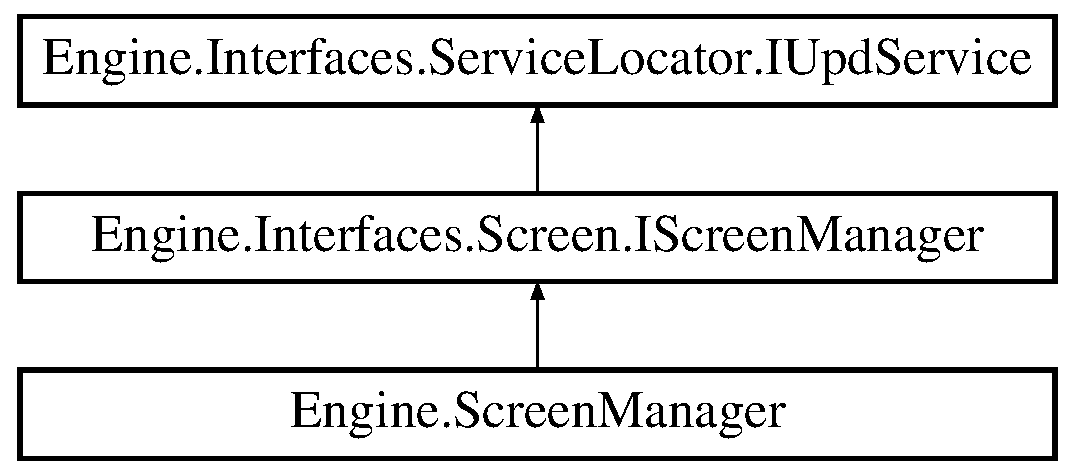
\includegraphics[height=3.000000cm]{dd/d5a/a00538}
\end{center}
\end{figure}
\subsection*{Public Member Functions}
\begin{DoxyCompactItemize}
\item 
delegate void \hyperlink{a00538_ad442d9999cb6f335509f21ddb533bd76}{s\+Manager\+Event} (\hyperlink{a00550}{Base\+Screen} screen)
\item 
void \hyperlink{a00538_aaa2b6fe0b50cf126bbb0a9b39fac1b83}{Initialize} ()
\begin{DoxyCompactList}\small\item\em Initialize the screenmanager and add the menu to the stack to start the game off. Soon this will be replaced with a splashscreen which will transition to the menu \end{DoxyCompactList}\item 
void \hyperlink{a00538_a1e85d6cc74fdb929f4729d1170886fb4}{Unlo\+Enginecreens} ()
\begin{DoxyCompactList}\small\item\em Unload any screens which need to be unloaded \end{DoxyCompactList}\item 
void \hyperlink{a00538_a9abaa968b161ebb2b84c7a47ada52f90}{Update} (Game\+Time game\+Time)
\begin{DoxyCompactList}\small\item\em M\+E\+T\+H\+OD\+: Update the manager \end{DoxyCompactList}\item 
void \hyperlink{a00538_a1177fbd3eb0a300167e4fa99930025e1}{Draw} (Sprite\+Batch sprite\+Batch)
\begin{DoxyCompactList}\small\item\em Currently draws the topmost screen, needs to be improved to support things such as pop ups It\textquotesingle{}ll be a simple fix to check to see which screens are requesting to be drawn and draw them in the order of the stack. \end{DoxyCompactList}\item 
void \hyperlink{a00538_ae459e146f1e05789c4d5828cca4dead7}{Add} (string screen\+Name)
\begin{DoxyCompactList}\small\item\em This method is self explanitory, it asks for the class name you wish to add to the screenstack and pushes it onto the top. \end{DoxyCompactList}\item 
void \hyperlink{a00538_a28af5b838f4345834dc2351e06c3d654}{Replace\+Screen} (string screen\+Name)
\begin{DoxyCompactList}\small\item\em This method is similar to the add method, but rather than just removing the screen to go back to the previous screen, this method replaces a screen (If you wanted to replace level1 with level2 \end{DoxyCompactList}\item 
void \hyperlink{a00538_abe1bf121b368a6d205706da54d949ace}{Check\+Screens} ()
\begin{DoxyCompactList}\small\item\em Checks each of the screens in the screenstack and checks if its the same screen as the current screen if so then declare the screen active, ready for drawing and updating. \end{DoxyCompactList}\item 
void \hyperlink{a00538_aa8e3ecdc7ae78094b07af944c31f90a9}{Check\+Screen\+Manager\+Input} ()
\begin{DoxyCompactList}\small\item\em Checks for input, more specifically if the E\+S\+C\+A\+PE key has been pressed and if the screen count is more than 1, go back a screen. Otherwise there will be no screens present and the screenmanager will be broken. \end{DoxyCompactList}\item 
void \hyperlink{a00538_ab553bead481adc65547a323af9dab2d5}{Remove\+Top\+Screen} ()
\begin{DoxyCompactList}\small\item\em Removes the top screen from the stack. Should be used in situations such as if the er has lost all of his lives and the state should be reverted back to the menu screen this will be your god. It basically goes back one screen \+:) \end{DoxyCompactList}\item 
void \hyperlink{a00538_a59b04e135a3b2a75a608752e2bfabc77}{Update\+Top\+Screen} (Game\+Time game\+Time)
\begin{DoxyCompactList}\small\item\em This is probably the worst way of going about it but this method checks the top screen and updates it Although this will not be relevant soon since screen updates will be decided through E\+N\+U\+MS. \end{DoxyCompactList}\end{DoxyCompactItemize}
\subsection*{Protected Member Functions}
\begin{DoxyCompactItemize}
\item 
virtual void \hyperlink{a00538_a973c15b5fff9fb873ed988ea69ccbfd1}{on\+Screen\+Change} (\hyperlink{a00550}{Base\+Screen} screen)
\end{DoxyCompactItemize}
\subsection*{Properties}
\begin{DoxyCompactItemize}
\item 
Content\+Manager \hyperlink{a00538_aab6681c2803637c394081f3132dd2846}{content}\hspace{0.3cm}{\ttfamily  \mbox{[}get, set\mbox{]}}
\item 
List$<$ \hyperlink{a00438}{I\+Entity} $>$ \hyperlink{a00538_a8fb99d85abd848bad9d850b742398801}{Entity\+List}\hspace{0.3cm}{\ttfamily  \mbox{[}get, set\mbox{]}}
\end{DoxyCompactItemize}
\subsection*{Events}
\begin{DoxyCompactItemize}
\item 
\hyperlink{a00538_ad442d9999cb6f335509f21ddb533bd76}{s\+Manager\+Event} \hyperlink{a00538_ab29ea82cff043c98756eaa9f538a72e7}{Screen\+Change}
\end{DoxyCompactItemize}


\subsection{Member Function Documentation}
\mbox{\Hypertarget{a00538_ae459e146f1e05789c4d5828cca4dead7}\label{a00538_ae459e146f1e05789c4d5828cca4dead7}} 
\index{Engine\+::\+Screen\+Manager@{Engine\+::\+Screen\+Manager}!Add@{Add}}
\index{Add@{Add}!Engine\+::\+Screen\+Manager@{Engine\+::\+Screen\+Manager}}
\subsubsection{\texorpdfstring{Add()}{Add()}}
{\footnotesize\ttfamily void Engine.\+Screen\+Manager.\+Add (\begin{DoxyParamCaption}\item[{string}]{screen\+Name }\end{DoxyParamCaption})\hspace{0.3cm}{\ttfamily [inline]}}



This method is self explanitory, it asks for the class name you wish to add to the screenstack and pushes it onto the top. 


\begin{DoxyParams}{Parameters}
{\em screen\+Name} & \\
\hline
\end{DoxyParams}


Implements \hyperlink{a00470_aba0b8f29600dabc2a55dde4d5e00c7bc}{Engine.\+Interfaces.\+Screen.\+I\+Screen\+Manager}.

\mbox{\Hypertarget{a00538_aa8e3ecdc7ae78094b07af944c31f90a9}\label{a00538_aa8e3ecdc7ae78094b07af944c31f90a9}} 
\index{Engine\+::\+Screen\+Manager@{Engine\+::\+Screen\+Manager}!Check\+Screen\+Manager\+Input@{Check\+Screen\+Manager\+Input}}
\index{Check\+Screen\+Manager\+Input@{Check\+Screen\+Manager\+Input}!Engine\+::\+Screen\+Manager@{Engine\+::\+Screen\+Manager}}
\subsubsection{\texorpdfstring{Check\+Screen\+Manager\+Input()}{CheckScreenManagerInput()}}
{\footnotesize\ttfamily void Engine.\+Screen\+Manager.\+Check\+Screen\+Manager\+Input (\begin{DoxyParamCaption}{ }\end{DoxyParamCaption})\hspace{0.3cm}{\ttfamily [inline]}}



Checks for input, more specifically if the E\+S\+C\+A\+PE key has been pressed and if the screen count is more than 1, go back a screen. Otherwise there will be no screens present and the screenmanager will be broken. 



Implements \hyperlink{a00470_a833b8050119cd9a87efbfa23197457c9}{Engine.\+Interfaces.\+Screen.\+I\+Screen\+Manager}.

\mbox{\Hypertarget{a00538_abe1bf121b368a6d205706da54d949ace}\label{a00538_abe1bf121b368a6d205706da54d949ace}} 
\index{Engine\+::\+Screen\+Manager@{Engine\+::\+Screen\+Manager}!Check\+Screens@{Check\+Screens}}
\index{Check\+Screens@{Check\+Screens}!Engine\+::\+Screen\+Manager@{Engine\+::\+Screen\+Manager}}
\subsubsection{\texorpdfstring{Check\+Screens()}{CheckScreens()}}
{\footnotesize\ttfamily void Engine.\+Screen\+Manager.\+Check\+Screens (\begin{DoxyParamCaption}{ }\end{DoxyParamCaption})\hspace{0.3cm}{\ttfamily [inline]}}



Checks each of the screens in the screenstack and checks if its the same screen as the current screen if so then declare the screen active, ready for drawing and updating. 

TO DO

Give screens individual I\+Ds just like entities. 

Implements \hyperlink{a00470_a40fbf0a98c186ba93837f6279ad2f7dd}{Engine.\+Interfaces.\+Screen.\+I\+Screen\+Manager}.

\mbox{\Hypertarget{a00538_a1177fbd3eb0a300167e4fa99930025e1}\label{a00538_a1177fbd3eb0a300167e4fa99930025e1}} 
\index{Engine\+::\+Screen\+Manager@{Engine\+::\+Screen\+Manager}!Draw@{Draw}}
\index{Draw@{Draw}!Engine\+::\+Screen\+Manager@{Engine\+::\+Screen\+Manager}}
\subsubsection{\texorpdfstring{Draw()}{Draw()}}
{\footnotesize\ttfamily void Engine.\+Screen\+Manager.\+Draw (\begin{DoxyParamCaption}\item[{Sprite\+Batch}]{sprite\+Batch }\end{DoxyParamCaption})\hspace{0.3cm}{\ttfamily [inline]}}



Currently draws the topmost screen, needs to be improved to support things such as pop ups It\textquotesingle{}ll be a simple fix to check to see which screens are requesting to be drawn and draw them in the order of the stack. 


\begin{DoxyParams}{Parameters}
{\em sprite\+Batch} & \\
\hline
\end{DoxyParams}


Implements \hyperlink{a00470_a28a87245d63c8df1634598b3d20a14cf}{Engine.\+Interfaces.\+Screen.\+I\+Screen\+Manager}.

\mbox{\Hypertarget{a00538_aaa2b6fe0b50cf126bbb0a9b39fac1b83}\label{a00538_aaa2b6fe0b50cf126bbb0a9b39fac1b83}} 
\index{Engine\+::\+Screen\+Manager@{Engine\+::\+Screen\+Manager}!Initialize@{Initialize}}
\index{Initialize@{Initialize}!Engine\+::\+Screen\+Manager@{Engine\+::\+Screen\+Manager}}
\subsubsection{\texorpdfstring{Initialize()}{Initialize()}}
{\footnotesize\ttfamily void Engine.\+Screen\+Manager.\+Initialize (\begin{DoxyParamCaption}{ }\end{DoxyParamCaption})\hspace{0.3cm}{\ttfamily [inline]}}



Initialize the screenmanager and add the menu to the stack to start the game off. Soon this will be replaced with a splashscreen which will transition to the menu 



Implements \hyperlink{a00470_ae37c13c038cdb202262013731985eb10}{Engine.\+Interfaces.\+Screen.\+I\+Screen\+Manager}.

\mbox{\Hypertarget{a00538_a973c15b5fff9fb873ed988ea69ccbfd1}\label{a00538_a973c15b5fff9fb873ed988ea69ccbfd1}} 
\index{Engine\+::\+Screen\+Manager@{Engine\+::\+Screen\+Manager}!on\+Screen\+Change@{on\+Screen\+Change}}
\index{on\+Screen\+Change@{on\+Screen\+Change}!Engine\+::\+Screen\+Manager@{Engine\+::\+Screen\+Manager}}
\subsubsection{\texorpdfstring{on\+Screen\+Change()}{onScreenChange()}}
{\footnotesize\ttfamily virtual void Engine.\+Screen\+Manager.\+on\+Screen\+Change (\begin{DoxyParamCaption}\item[{\hyperlink{a00550}{Base\+Screen}}]{screen }\end{DoxyParamCaption})\hspace{0.3cm}{\ttfamily [inline]}, {\ttfamily [protected]}, {\ttfamily [virtual]}}

\mbox{\Hypertarget{a00538_ab553bead481adc65547a323af9dab2d5}\label{a00538_ab553bead481adc65547a323af9dab2d5}} 
\index{Engine\+::\+Screen\+Manager@{Engine\+::\+Screen\+Manager}!Remove\+Top\+Screen@{Remove\+Top\+Screen}}
\index{Remove\+Top\+Screen@{Remove\+Top\+Screen}!Engine\+::\+Screen\+Manager@{Engine\+::\+Screen\+Manager}}
\subsubsection{\texorpdfstring{Remove\+Top\+Screen()}{RemoveTopScreen()}}
{\footnotesize\ttfamily void Engine.\+Screen\+Manager.\+Remove\+Top\+Screen (\begin{DoxyParamCaption}{ }\end{DoxyParamCaption})\hspace{0.3cm}{\ttfamily [inline]}}



Removes the top screen from the stack. Should be used in situations such as if the er has lost all of his lives and the state should be reverted back to the menu screen this will be your god. It basically goes back one screen \+:) 



Implements \hyperlink{a00470_a91b5204271edf5e137a85d3f8f3876d8}{Engine.\+Interfaces.\+Screen.\+I\+Screen\+Manager}.

\mbox{\Hypertarget{a00538_a28af5b838f4345834dc2351e06c3d654}\label{a00538_a28af5b838f4345834dc2351e06c3d654}} 
\index{Engine\+::\+Screen\+Manager@{Engine\+::\+Screen\+Manager}!Replace\+Screen@{Replace\+Screen}}
\index{Replace\+Screen@{Replace\+Screen}!Engine\+::\+Screen\+Manager@{Engine\+::\+Screen\+Manager}}
\subsubsection{\texorpdfstring{Replace\+Screen()}{ReplaceScreen()}}
{\footnotesize\ttfamily void Engine.\+Screen\+Manager.\+Replace\+Screen (\begin{DoxyParamCaption}\item[{string}]{screen\+Name }\end{DoxyParamCaption})\hspace{0.3cm}{\ttfamily [inline]}}



This method is similar to the add method, but rather than just removing the screen to go back to the previous screen, this method replaces a screen (If you wanted to replace level1 with level2 


\begin{DoxyParams}{Parameters}
{\em screen\+Name} & \\
\hline
\end{DoxyParams}


Implements \hyperlink{a00470_aaa6bfa9a986729ada7dcea6ac40f078d}{Engine.\+Interfaces.\+Screen.\+I\+Screen\+Manager}.

\mbox{\Hypertarget{a00538_ad442d9999cb6f335509f21ddb533bd76}\label{a00538_ad442d9999cb6f335509f21ddb533bd76}} 
\index{Engine\+::\+Screen\+Manager@{Engine\+::\+Screen\+Manager}!s\+Manager\+Event@{s\+Manager\+Event}}
\index{s\+Manager\+Event@{s\+Manager\+Event}!Engine\+::\+Screen\+Manager@{Engine\+::\+Screen\+Manager}}
\subsubsection{\texorpdfstring{s\+Manager\+Event()}{sManagerEvent()}}
{\footnotesize\ttfamily delegate void Engine.\+Screen\+Manager.\+s\+Manager\+Event (\begin{DoxyParamCaption}\item[{\hyperlink{a00550}{Base\+Screen}}]{screen }\end{DoxyParamCaption})}

\mbox{\Hypertarget{a00538_a1e85d6cc74fdb929f4729d1170886fb4}\label{a00538_a1e85d6cc74fdb929f4729d1170886fb4}} 
\index{Engine\+::\+Screen\+Manager@{Engine\+::\+Screen\+Manager}!Unlo\+Enginecreens@{Unlo\+Enginecreens}}
\index{Unlo\+Enginecreens@{Unlo\+Enginecreens}!Engine\+::\+Screen\+Manager@{Engine\+::\+Screen\+Manager}}
\subsubsection{\texorpdfstring{Unlo\+Enginecreens()}{UnloEnginecreens()}}
{\footnotesize\ttfamily void Engine.\+Screen\+Manager.\+Unlo\+Enginecreens (\begin{DoxyParamCaption}{ }\end{DoxyParamCaption})\hspace{0.3cm}{\ttfamily [inline]}}



Unload any screens which need to be unloaded 



Implements \hyperlink{a00470_a8d30874c7b1b2728a784de0c6e6f80e3}{Engine.\+Interfaces.\+Screen.\+I\+Screen\+Manager}.

\mbox{\Hypertarget{a00538_a9abaa968b161ebb2b84c7a47ada52f90}\label{a00538_a9abaa968b161ebb2b84c7a47ada52f90}} 
\index{Engine\+::\+Screen\+Manager@{Engine\+::\+Screen\+Manager}!Update@{Update}}
\index{Update@{Update}!Engine\+::\+Screen\+Manager@{Engine\+::\+Screen\+Manager}}
\subsubsection{\texorpdfstring{Update()}{Update()}}
{\footnotesize\ttfamily void Engine.\+Screen\+Manager.\+Update (\begin{DoxyParamCaption}\item[{Game\+Time}]{game\+Time }\end{DoxyParamCaption})\hspace{0.3cm}{\ttfamily [inline]}}



M\+E\+T\+H\+OD\+: Update the manager 


\begin{DoxyParams}{Parameters}
{\em game\+Time} & Monogame Game\+Time property\\
\hline
\end{DoxyParams}


Implements \hyperlink{a00470_afc42708b653397ca8a3a81dc8d244c61}{Engine.\+Interfaces.\+Screen.\+I\+Screen\+Manager}.

\mbox{\Hypertarget{a00538_a59b04e135a3b2a75a608752e2bfabc77}\label{a00538_a59b04e135a3b2a75a608752e2bfabc77}} 
\index{Engine\+::\+Screen\+Manager@{Engine\+::\+Screen\+Manager}!Update\+Top\+Screen@{Update\+Top\+Screen}}
\index{Update\+Top\+Screen@{Update\+Top\+Screen}!Engine\+::\+Screen\+Manager@{Engine\+::\+Screen\+Manager}}
\subsubsection{\texorpdfstring{Update\+Top\+Screen()}{UpdateTopScreen()}}
{\footnotesize\ttfamily void Engine.\+Screen\+Manager.\+Update\+Top\+Screen (\begin{DoxyParamCaption}\item[{Game\+Time}]{game\+Time }\end{DoxyParamCaption})\hspace{0.3cm}{\ttfamily [inline]}}



This is probably the worst way of going about it but this method checks the top screen and updates it Although this will not be relevant soon since screen updates will be decided through E\+N\+U\+MS. 


\begin{DoxyParams}{Parameters}
{\em game\+Time} & \\
\hline
\end{DoxyParams}


Implements \hyperlink{a00470_aff4347b40d3fd6173e0c420adbf1146f}{Engine.\+Interfaces.\+Screen.\+I\+Screen\+Manager}.



\subsection{Property Documentation}
\mbox{\Hypertarget{a00538_aab6681c2803637c394081f3132dd2846}\label{a00538_aab6681c2803637c394081f3132dd2846}} 
\index{Engine\+::\+Screen\+Manager@{Engine\+::\+Screen\+Manager}!content@{content}}
\index{content@{content}!Engine\+::\+Screen\+Manager@{Engine\+::\+Screen\+Manager}}
\subsubsection{\texorpdfstring{content}{content}}
{\footnotesize\ttfamily Content\+Manager Engine.\+Screen\+Manager.\+content\hspace{0.3cm}{\ttfamily [get]}, {\ttfamily [set]}}

\mbox{\Hypertarget{a00538_a8fb99d85abd848bad9d850b742398801}\label{a00538_a8fb99d85abd848bad9d850b742398801}} 
\index{Engine\+::\+Screen\+Manager@{Engine\+::\+Screen\+Manager}!Entity\+List@{Entity\+List}}
\index{Entity\+List@{Entity\+List}!Engine\+::\+Screen\+Manager@{Engine\+::\+Screen\+Manager}}
\subsubsection{\texorpdfstring{Entity\+List}{EntityList}}
{\footnotesize\ttfamily List$<$\hyperlink{a00438}{I\+Entity}$>$ Engine.\+Screen\+Manager.\+Entity\+List\hspace{0.3cm}{\ttfamily [get]}, {\ttfamily [set]}}



\subsection{Event Documentation}
\mbox{\Hypertarget{a00538_ab29ea82cff043c98756eaa9f538a72e7}\label{a00538_ab29ea82cff043c98756eaa9f538a72e7}} 
\index{Engine\+::\+Screen\+Manager@{Engine\+::\+Screen\+Manager}!Screen\+Change@{Screen\+Change}}
\index{Screen\+Change@{Screen\+Change}!Engine\+::\+Screen\+Manager@{Engine\+::\+Screen\+Manager}}
\subsubsection{\texorpdfstring{Screen\+Change}{ScreenChange}}
{\footnotesize\ttfamily \hyperlink{a00538_ad442d9999cb6f335509f21ddb533bd76}{s\+Manager\+Event} Engine.\+Screen\+Manager.\+Screen\+Change}



The documentation for this class was generated from the following file\+:\begin{DoxyCompactItemize}
\item 
\hyperlink{a00185}{Screen\+Manager.\+cs}\end{DoxyCompactItemize}

\hypertarget{a00386}{}\section{Engine.\+Events.\+Screen\+Event.\+s\+Manager\+Args Class Reference}
\label{a00386}\index{Engine.\+Events.\+Screen\+Event.\+s\+Manager\+Args@{Engine.\+Events.\+Screen\+Event.\+s\+Manager\+Args}}


The documentation for this class was generated from the following file\+:\begin{DoxyCompactItemize}
\item 
\hyperlink{a00071}{s\+Manager\+Args.\+cs}\end{DoxyCompactItemize}

\hypertarget{a00390}{}\section{Engine.\+Events.\+Sound\+Event.\+Sound\+Event\+Args Class Reference}
\label{a00390}\index{Engine.\+Events.\+Sound\+Event.\+Sound\+Event\+Args@{Engine.\+Events.\+Sound\+Event.\+Sound\+Event\+Args}}


The documentation for this class was generated from the following file\+:\begin{DoxyCompactItemize}
\item 
\hyperlink{a00074}{Sound\+Event\+Args.\+cs}\end{DoxyCompactItemize}

\hypertarget{a00394}{}\section{Engine.\+Events.\+Sound\+Event.\+Sound\+Handler Class Reference}
\label{a00394}\index{Engine.\+Events.\+Sound\+Event.\+Sound\+Handler@{Engine.\+Events.\+Sound\+Event.\+Sound\+Handler}}


The documentation for this class was generated from the following file\+:\begin{DoxyCompactItemize}
\item 
\hyperlink{a00077}{Sound\+Handler.\+cs}\end{DoxyCompactItemize}

\hypertarget{a00546}{}\section{Engine.\+Managers.\+Sound.\+Sound\+Manager Class Reference}
\label{a00546}\index{Engine.\+Managers.\+Sound.\+Sound\+Manager@{Engine.\+Managers.\+Sound.\+Sound\+Manager}}


C\+L\+A\+SS\+: The sound manager is responsible for the storage and playback of sound files  


Inheritance diagram for Engine.\+Managers.\+Sound.\+Sound\+Manager\+:\begin{figure}[H]
\begin{center}
\leavevmode
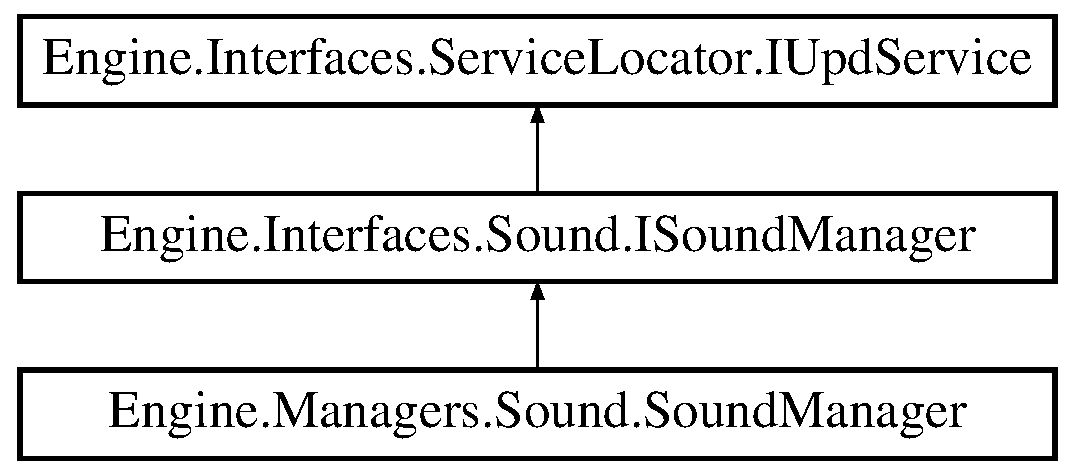
\includegraphics[height=3.000000cm]{dc/d2b/a00546}
\end{center}
\end{figure}
\subsection*{Public Member Functions}
\begin{DoxyCompactItemize}
\item 
void \hyperlink{a00546_a06224065983b6fe162de98b8dcc944c2}{Initialize} ()
\begin{DoxyCompactList}\small\item\em M\+E\+T\+H\+OD\+: Initialise the Monogame Media\+Player and \hyperlink{a00538}{Screen\+Manager} \end{DoxyCompactList}\item 
void \hyperlink{a00546_aabfeb911d8bd573065e9c02d3f81e582}{Play} (string name)
\begin{DoxyCompactList}\small\item\em M\+E\+T\+H\+OD\+: Play a song that is located within the resource loaders song library \end{DoxyCompactList}\item 
void \hyperlink{a00546_a6613813ccd38703484e80ca8775ecdf8}{Play\+Effect} (string name)
\begin{DoxyCompactList}\small\item\em M\+E\+T\+H\+OD\+: Plays the sound effect of the name provided \end{DoxyCompactList}\item 
void \hyperlink{a00546_a5a3a9b96e6708deedf2c4939b3259011}{Mute} ()
\begin{DoxyCompactList}\small\item\em M\+E\+T\+H\+OD\+: Mutes all sound \end{DoxyCompactList}\item 
void \hyperlink{a00546_ad62eb34a308bfe457bc7229045a66af0}{un\+Mute} ()
\begin{DoxyCompactList}\small\item\em M\+E\+T\+H\+OD\+: Unmutes all sound \end{DoxyCompactList}\item 
void \hyperlink{a00546_ae1be3ecb76007fdc47843305df49604b}{Volume} (float Volume)
\begin{DoxyCompactList}\small\item\em M\+E\+T\+H\+OD\+: Adjust the volume of sound playback \end{DoxyCompactList}\item 
void \hyperlink{a00546_a0d3222475855f63b0c8f9dbe9b52e7f7}{Stop} ()
\begin{DoxyCompactList}\small\item\em M\+E\+T\+H\+OD\+: Stop playback \end{DoxyCompactList}\item 
void \hyperlink{a00546_a43e47a47daa91f3b1d0f38b3dcb0323e}{Update} (Game\+Time game\+Time)
\begin{DoxyCompactList}\small\item\em M\+E\+T\+H\+OD\+: the update loop cycled through each frame \end{DoxyCompactList}\item 
void \hyperlink{a00546_af9d82c533dfd90077b275f2b09ee90b0}{vol\+Up} ()
\begin{DoxyCompactList}\small\item\em M\+E\+T\+H\+OD\+: Increases the volume slightly \end{DoxyCompactList}\item 
void \hyperlink{a00546_a888a7942f63cc582f7b73d61b69ebbac}{vol\+Down} ()
\begin{DoxyCompactList}\small\item\em M\+E\+T\+H\+OD\+: Decreases the volume slightly \end{DoxyCompactList}\item 
void \hyperlink{a00546_a8dfbb15525871b87e6cdcf744b070139}{on\+Screen\+Changed} (\hyperlink{a00550}{Base\+Screen} screen)
\begin{DoxyCompactList}\small\item\em M\+E\+T\+H\+OD\+: Plays the sound of the screen that is being changed to \end{DoxyCompactList}\end{DoxyCompactItemize}
\subsection*{Properties}
\begin{DoxyCompactItemize}
\item 
bool \hyperlink{a00546_a2a4a319a1d395e58c2b10f393475a0c9}{is\+Muted}\hspace{0.3cm}{\ttfamily  \mbox{[}get, set\mbox{]}}
\end{DoxyCompactItemize}


\subsection{Detailed Description}
C\+L\+A\+SS\+: The sound manager is responsible for the storage and playback of sound files 



\subsection{Member Function Documentation}
\mbox{\Hypertarget{a00546_a06224065983b6fe162de98b8dcc944c2}\label{a00546_a06224065983b6fe162de98b8dcc944c2}} 
\index{Engine\+::\+Managers\+::\+Sound\+::\+Sound\+Manager@{Engine\+::\+Managers\+::\+Sound\+::\+Sound\+Manager}!Initialize@{Initialize}}
\index{Initialize@{Initialize}!Engine\+::\+Managers\+::\+Sound\+::\+Sound\+Manager@{Engine\+::\+Managers\+::\+Sound\+::\+Sound\+Manager}}
\subsubsection{\texorpdfstring{Initialize()}{Initialize()}}
{\footnotesize\ttfamily void Engine.\+Managers.\+Sound.\+Sound\+Manager.\+Initialize (\begin{DoxyParamCaption}{ }\end{DoxyParamCaption})\hspace{0.3cm}{\ttfamily [inline]}}



M\+E\+T\+H\+OD\+: Initialise the Monogame Media\+Player and \hyperlink{a00538}{Screen\+Manager} 



Implements \hyperlink{a00482_a02f14f3401f425a686a50e6b6a40aca7}{Engine.\+Interfaces.\+Sound.\+I\+Sound\+Manager}.

\mbox{\Hypertarget{a00546_a5a3a9b96e6708deedf2c4939b3259011}\label{a00546_a5a3a9b96e6708deedf2c4939b3259011}} 
\index{Engine\+::\+Managers\+::\+Sound\+::\+Sound\+Manager@{Engine\+::\+Managers\+::\+Sound\+::\+Sound\+Manager}!Mute@{Mute}}
\index{Mute@{Mute}!Engine\+::\+Managers\+::\+Sound\+::\+Sound\+Manager@{Engine\+::\+Managers\+::\+Sound\+::\+Sound\+Manager}}
\subsubsection{\texorpdfstring{Mute()}{Mute()}}
{\footnotesize\ttfamily void Engine.\+Managers.\+Sound.\+Sound\+Manager.\+Mute (\begin{DoxyParamCaption}{ }\end{DoxyParamCaption})\hspace{0.3cm}{\ttfamily [inline]}}



M\+E\+T\+H\+OD\+: Mutes all sound 



Implements \hyperlink{a00482_a5bcad4d517b37a12b17e59d0b927ca37}{Engine.\+Interfaces.\+Sound.\+I\+Sound\+Manager}.

\mbox{\Hypertarget{a00546_a8dfbb15525871b87e6cdcf744b070139}\label{a00546_a8dfbb15525871b87e6cdcf744b070139}} 
\index{Engine\+::\+Managers\+::\+Sound\+::\+Sound\+Manager@{Engine\+::\+Managers\+::\+Sound\+::\+Sound\+Manager}!on\+Screen\+Changed@{on\+Screen\+Changed}}
\index{on\+Screen\+Changed@{on\+Screen\+Changed}!Engine\+::\+Managers\+::\+Sound\+::\+Sound\+Manager@{Engine\+::\+Managers\+::\+Sound\+::\+Sound\+Manager}}
\subsubsection{\texorpdfstring{on\+Screen\+Changed()}{onScreenChanged()}}
{\footnotesize\ttfamily void Engine.\+Managers.\+Sound.\+Sound\+Manager.\+on\+Screen\+Changed (\begin{DoxyParamCaption}\item[{\hyperlink{a00550}{Base\+Screen}}]{screen }\end{DoxyParamCaption})\hspace{0.3cm}{\ttfamily [inline]}}



M\+E\+T\+H\+OD\+: Plays the sound of the screen that is being changed to 


\begin{DoxyParams}{Parameters}
{\em screen} & The screen being changed to\\
\hline
\end{DoxyParams}


Implements \hyperlink{a00482_a8aa47dcffde058c1146f7ebf5b0edb84}{Engine.\+Interfaces.\+Sound.\+I\+Sound\+Manager}.

\mbox{\Hypertarget{a00546_aabfeb911d8bd573065e9c02d3f81e582}\label{a00546_aabfeb911d8bd573065e9c02d3f81e582}} 
\index{Engine\+::\+Managers\+::\+Sound\+::\+Sound\+Manager@{Engine\+::\+Managers\+::\+Sound\+::\+Sound\+Manager}!Play@{Play}}
\index{Play@{Play}!Engine\+::\+Managers\+::\+Sound\+::\+Sound\+Manager@{Engine\+::\+Managers\+::\+Sound\+::\+Sound\+Manager}}
\subsubsection{\texorpdfstring{Play()}{Play()}}
{\footnotesize\ttfamily void Engine.\+Managers.\+Sound.\+Sound\+Manager.\+Play (\begin{DoxyParamCaption}\item[{string}]{name }\end{DoxyParamCaption})\hspace{0.3cm}{\ttfamily [inline]}}



M\+E\+T\+H\+OD\+: Play a song that is located within the resource loaders song library 


\begin{DoxyParams}{Parameters}
{\em name} & Name of the sound file to be played\\
\hline
\end{DoxyParams}


Implements \hyperlink{a00482_aec02346c5397b9b01b9d5d6baedc923e}{Engine.\+Interfaces.\+Sound.\+I\+Sound\+Manager}.

\mbox{\Hypertarget{a00546_a6613813ccd38703484e80ca8775ecdf8}\label{a00546_a6613813ccd38703484e80ca8775ecdf8}} 
\index{Engine\+::\+Managers\+::\+Sound\+::\+Sound\+Manager@{Engine\+::\+Managers\+::\+Sound\+::\+Sound\+Manager}!Play\+Effect@{Play\+Effect}}
\index{Play\+Effect@{Play\+Effect}!Engine\+::\+Managers\+::\+Sound\+::\+Sound\+Manager@{Engine\+::\+Managers\+::\+Sound\+::\+Sound\+Manager}}
\subsubsection{\texorpdfstring{Play\+Effect()}{PlayEffect()}}
{\footnotesize\ttfamily void Engine.\+Managers.\+Sound.\+Sound\+Manager.\+Play\+Effect (\begin{DoxyParamCaption}\item[{string}]{name }\end{DoxyParamCaption})\hspace{0.3cm}{\ttfamily [inline]}}



M\+E\+T\+H\+OD\+: Plays the sound effect of the name provided 


\begin{DoxyParams}{Parameters}
{\em name} & The name of the sound effect to be played\\
\hline
\end{DoxyParams}


Implements \hyperlink{a00482_aa9e2fb77a5fe624ce65373f5ee8328ae}{Engine.\+Interfaces.\+Sound.\+I\+Sound\+Manager}.

\mbox{\Hypertarget{a00546_a0d3222475855f63b0c8f9dbe9b52e7f7}\label{a00546_a0d3222475855f63b0c8f9dbe9b52e7f7}} 
\index{Engine\+::\+Managers\+::\+Sound\+::\+Sound\+Manager@{Engine\+::\+Managers\+::\+Sound\+::\+Sound\+Manager}!Stop@{Stop}}
\index{Stop@{Stop}!Engine\+::\+Managers\+::\+Sound\+::\+Sound\+Manager@{Engine\+::\+Managers\+::\+Sound\+::\+Sound\+Manager}}
\subsubsection{\texorpdfstring{Stop()}{Stop()}}
{\footnotesize\ttfamily void Engine.\+Managers.\+Sound.\+Sound\+Manager.\+Stop (\begin{DoxyParamCaption}{ }\end{DoxyParamCaption})\hspace{0.3cm}{\ttfamily [inline]}}



M\+E\+T\+H\+OD\+: Stop playback 



Implements \hyperlink{a00482_ac47a91d3e28a8f7a1e5348fb6eff50e2}{Engine.\+Interfaces.\+Sound.\+I\+Sound\+Manager}.

\mbox{\Hypertarget{a00546_ad62eb34a308bfe457bc7229045a66af0}\label{a00546_ad62eb34a308bfe457bc7229045a66af0}} 
\index{Engine\+::\+Managers\+::\+Sound\+::\+Sound\+Manager@{Engine\+::\+Managers\+::\+Sound\+::\+Sound\+Manager}!un\+Mute@{un\+Mute}}
\index{un\+Mute@{un\+Mute}!Engine\+::\+Managers\+::\+Sound\+::\+Sound\+Manager@{Engine\+::\+Managers\+::\+Sound\+::\+Sound\+Manager}}
\subsubsection{\texorpdfstring{un\+Mute()}{unMute()}}
{\footnotesize\ttfamily void Engine.\+Managers.\+Sound.\+Sound\+Manager.\+un\+Mute (\begin{DoxyParamCaption}{ }\end{DoxyParamCaption})\hspace{0.3cm}{\ttfamily [inline]}}



M\+E\+T\+H\+OD\+: Unmutes all sound 



Implements \hyperlink{a00482_a59c011a4cf667d6e967bddad50c7cb2f}{Engine.\+Interfaces.\+Sound.\+I\+Sound\+Manager}.

\mbox{\Hypertarget{a00546_a43e47a47daa91f3b1d0f38b3dcb0323e}\label{a00546_a43e47a47daa91f3b1d0f38b3dcb0323e}} 
\index{Engine\+::\+Managers\+::\+Sound\+::\+Sound\+Manager@{Engine\+::\+Managers\+::\+Sound\+::\+Sound\+Manager}!Update@{Update}}
\index{Update@{Update}!Engine\+::\+Managers\+::\+Sound\+::\+Sound\+Manager@{Engine\+::\+Managers\+::\+Sound\+::\+Sound\+Manager}}
\subsubsection{\texorpdfstring{Update()}{Update()}}
{\footnotesize\ttfamily void Engine.\+Managers.\+Sound.\+Sound\+Manager.\+Update (\begin{DoxyParamCaption}\item[{Game\+Time}]{game\+Time }\end{DoxyParamCaption})\hspace{0.3cm}{\ttfamily [inline]}}



M\+E\+T\+H\+OD\+: the update loop cycled through each frame 


\begin{DoxyParams}{Parameters}
{\em game\+Time} & Monogame Game\+Time property\\
\hline
\end{DoxyParams}


Implements \hyperlink{a00482_af7ddcb52a6283aa2cf4392c75d2a0cff}{Engine.\+Interfaces.\+Sound.\+I\+Sound\+Manager}.

\mbox{\Hypertarget{a00546_a888a7942f63cc582f7b73d61b69ebbac}\label{a00546_a888a7942f63cc582f7b73d61b69ebbac}} 
\index{Engine\+::\+Managers\+::\+Sound\+::\+Sound\+Manager@{Engine\+::\+Managers\+::\+Sound\+::\+Sound\+Manager}!vol\+Down@{vol\+Down}}
\index{vol\+Down@{vol\+Down}!Engine\+::\+Managers\+::\+Sound\+::\+Sound\+Manager@{Engine\+::\+Managers\+::\+Sound\+::\+Sound\+Manager}}
\subsubsection{\texorpdfstring{vol\+Down()}{volDown()}}
{\footnotesize\ttfamily void Engine.\+Managers.\+Sound.\+Sound\+Manager.\+vol\+Down (\begin{DoxyParamCaption}{ }\end{DoxyParamCaption})\hspace{0.3cm}{\ttfamily [inline]}}



M\+E\+T\+H\+OD\+: Decreases the volume slightly 



Implements \hyperlink{a00482_a96629b32d608ca84fe1a3624bece7f05}{Engine.\+Interfaces.\+Sound.\+I\+Sound\+Manager}.

\mbox{\Hypertarget{a00546_ae1be3ecb76007fdc47843305df49604b}\label{a00546_ae1be3ecb76007fdc47843305df49604b}} 
\index{Engine\+::\+Managers\+::\+Sound\+::\+Sound\+Manager@{Engine\+::\+Managers\+::\+Sound\+::\+Sound\+Manager}!Volume@{Volume}}
\index{Volume@{Volume}!Engine\+::\+Managers\+::\+Sound\+::\+Sound\+Manager@{Engine\+::\+Managers\+::\+Sound\+::\+Sound\+Manager}}
\subsubsection{\texorpdfstring{Volume()}{Volume()}}
{\footnotesize\ttfamily void Engine.\+Managers.\+Sound.\+Sound\+Manager.\+Volume (\begin{DoxyParamCaption}\item[{float}]{Volume }\end{DoxyParamCaption})\hspace{0.3cm}{\ttfamily [inline]}}



M\+E\+T\+H\+OD\+: Adjust the volume of sound playback 


\begin{DoxyParams}{Parameters}
{\em Volume} & The volume the playback will be set to play at\\
\hline
\end{DoxyParams}


Implements \hyperlink{a00482_ada3f38d5c50655b55f146ccdaf7c5967}{Engine.\+Interfaces.\+Sound.\+I\+Sound\+Manager}.

\mbox{\Hypertarget{a00546_af9d82c533dfd90077b275f2b09ee90b0}\label{a00546_af9d82c533dfd90077b275f2b09ee90b0}} 
\index{Engine\+::\+Managers\+::\+Sound\+::\+Sound\+Manager@{Engine\+::\+Managers\+::\+Sound\+::\+Sound\+Manager}!vol\+Up@{vol\+Up}}
\index{vol\+Up@{vol\+Up}!Engine\+::\+Managers\+::\+Sound\+::\+Sound\+Manager@{Engine\+::\+Managers\+::\+Sound\+::\+Sound\+Manager}}
\subsubsection{\texorpdfstring{vol\+Up()}{volUp()}}
{\footnotesize\ttfamily void Engine.\+Managers.\+Sound.\+Sound\+Manager.\+vol\+Up (\begin{DoxyParamCaption}{ }\end{DoxyParamCaption})\hspace{0.3cm}{\ttfamily [inline]}}



M\+E\+T\+H\+OD\+: Increases the volume slightly 



Implements \hyperlink{a00482_afe3eaaed21c8b64692bc338309ac4a4d}{Engine.\+Interfaces.\+Sound.\+I\+Sound\+Manager}.



\subsection{Property Documentation}
\mbox{\Hypertarget{a00546_a2a4a319a1d395e58c2b10f393475a0c9}\label{a00546_a2a4a319a1d395e58c2b10f393475a0c9}} 
\index{Engine\+::\+Managers\+::\+Sound\+::\+Sound\+Manager@{Engine\+::\+Managers\+::\+Sound\+::\+Sound\+Manager}!is\+Muted@{is\+Muted}}
\index{is\+Muted@{is\+Muted}!Engine\+::\+Managers\+::\+Sound\+::\+Sound\+Manager@{Engine\+::\+Managers\+::\+Sound\+::\+Sound\+Manager}}
\subsubsection{\texorpdfstring{is\+Muted}{isMuted}}
{\footnotesize\ttfamily bool Engine.\+Managers.\+Sound.\+Sound\+Manager.\+is\+Muted\hspace{0.3cm}{\ttfamily [get]}, {\ttfamily [set]}}



The documentation for this class was generated from the following file\+:\begin{DoxyCompactItemize}
\item 
\hyperlink{a00191}{Sound\+Manager.\+cs}\end{DoxyCompactItemize}

\hypertarget{a00554}{}\section{Engine.\+States.\+Engine.\+Splash\+Screen Class Reference}
\label{a00554}\index{Engine.\+States.\+Engine.\+Splash\+Screen@{Engine.\+States.\+Engine.\+Splash\+Screen}}


C\+L\+A\+SS\+: The splash screen that is loaded upon running the program whilst the main menu loads  


Inheritance diagram for Engine.\+States.\+Engine.\+Splash\+Screen\+:\begin{figure}[H]
\begin{center}
\leavevmode
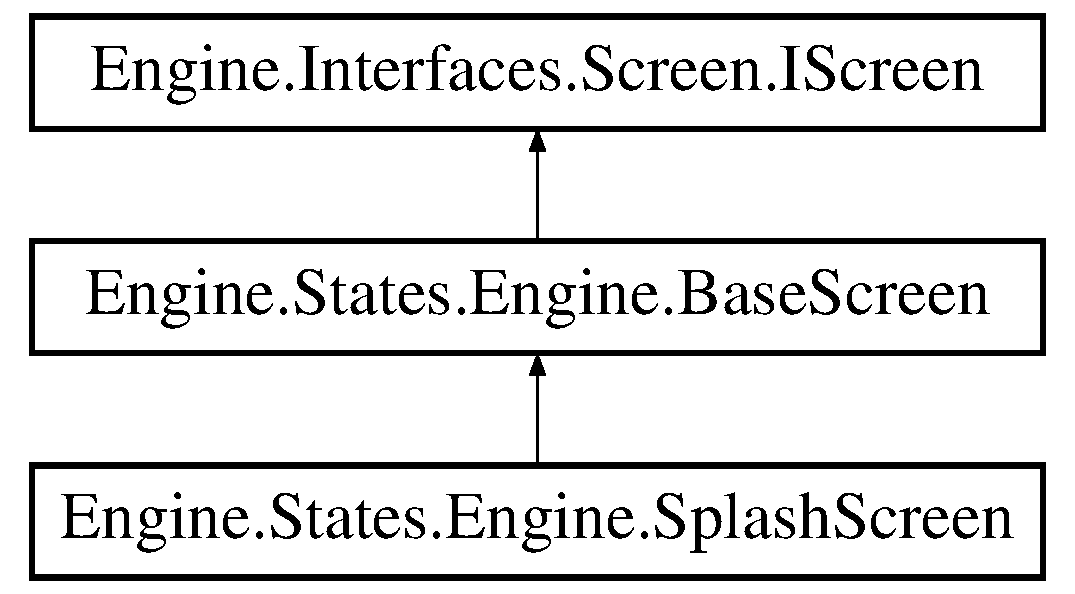
\includegraphics[height=3.000000cm]{dc/df9/a00554}
\end{center}
\end{figure}
\subsection*{Public Member Functions}
\begin{DoxyCompactItemize}
\item 
\hyperlink{a00554_a7f6973cb8b6b8fa31aace32fdd2dc260}{Splash\+Screen} ()
\begin{DoxyCompactList}\small\item\em C\+O\+N\+S\+T\+R\+U\+C\+T\+OR \end{DoxyCompactList}\item 
override void \hyperlink{a00554_a321c34cdc158a49cf76f31e3cdd0863e}{Initialize} ()
\begin{DoxyCompactList}\small\item\em M\+E\+T\+H\+OD\+: Initialises the logic for the splash screen \end{DoxyCompactList}\item 
override void \hyperlink{a00554_ae50fb213e5c1efc8d3908340b236e927}{Draw} (Sprite\+Batch sb)
\begin{DoxyCompactList}\small\item\em M\+E\+T\+H\+OD\+: Draws the screen content \end{DoxyCompactList}\item 
override void \hyperlink{a00554_af245506899484c6784a44550b1364b6c}{Update} (Game\+Time game\+Time)
\begin{DoxyCompactList}\small\item\em M\+E\+T\+H\+OD\+: Update which is cycled through each frame and contains the logic for the screen \end{DoxyCompactList}\end{DoxyCompactItemize}
\subsection*{Additional Inherited Members}


\subsection{Detailed Description}
C\+L\+A\+SS\+: The splash screen that is loaded upon running the program whilst the main menu loads 



\subsection{Constructor \& Destructor Documentation}
\mbox{\Hypertarget{a00554_a7f6973cb8b6b8fa31aace32fdd2dc260}\label{a00554_a7f6973cb8b6b8fa31aace32fdd2dc260}} 
\index{Engine\+::\+States\+::\+Engine\+::\+Splash\+Screen@{Engine\+::\+States\+::\+Engine\+::\+Splash\+Screen}!Splash\+Screen@{Splash\+Screen}}
\index{Splash\+Screen@{Splash\+Screen}!Engine\+::\+States\+::\+Engine\+::\+Splash\+Screen@{Engine\+::\+States\+::\+Engine\+::\+Splash\+Screen}}
\subsubsection{\texorpdfstring{Splash\+Screen()}{SplashScreen()}}
{\footnotesize\ttfamily Engine.\+States.\+Engine.\+Splash\+Screen.\+Splash\+Screen (\begin{DoxyParamCaption}{ }\end{DoxyParamCaption})\hspace{0.3cm}{\ttfamily [inline]}}



C\+O\+N\+S\+T\+R\+U\+C\+T\+OR 



\subsection{Member Function Documentation}
\mbox{\Hypertarget{a00554_ae50fb213e5c1efc8d3908340b236e927}\label{a00554_ae50fb213e5c1efc8d3908340b236e927}} 
\index{Engine\+::\+States\+::\+Engine\+::\+Splash\+Screen@{Engine\+::\+States\+::\+Engine\+::\+Splash\+Screen}!Draw@{Draw}}
\index{Draw@{Draw}!Engine\+::\+States\+::\+Engine\+::\+Splash\+Screen@{Engine\+::\+States\+::\+Engine\+::\+Splash\+Screen}}
\subsubsection{\texorpdfstring{Draw()}{Draw()}}
{\footnotesize\ttfamily override void Engine.\+States.\+Engine.\+Splash\+Screen.\+Draw (\begin{DoxyParamCaption}\item[{Sprite\+Batch}]{sb }\end{DoxyParamCaption})\hspace{0.3cm}{\ttfamily [inline]}, {\ttfamily [virtual]}}



M\+E\+T\+H\+OD\+: Draws the screen content 


\begin{DoxyParams}{Parameters}
{\em sb} & Monogame Sprite\+Batch\\
\hline
\end{DoxyParams}


Reimplemented from \hyperlink{a00550_a200c31954effe5fc060118607155fb16}{Engine.\+States.\+Engine.\+Base\+Screen}.

\mbox{\Hypertarget{a00554_a321c34cdc158a49cf76f31e3cdd0863e}\label{a00554_a321c34cdc158a49cf76f31e3cdd0863e}} 
\index{Engine\+::\+States\+::\+Engine\+::\+Splash\+Screen@{Engine\+::\+States\+::\+Engine\+::\+Splash\+Screen}!Initialize@{Initialize}}
\index{Initialize@{Initialize}!Engine\+::\+States\+::\+Engine\+::\+Splash\+Screen@{Engine\+::\+States\+::\+Engine\+::\+Splash\+Screen}}
\subsubsection{\texorpdfstring{Initialize()}{Initialize()}}
{\footnotesize\ttfamily override void Engine.\+States.\+Engine.\+Splash\+Screen.\+Initialize (\begin{DoxyParamCaption}{ }\end{DoxyParamCaption})\hspace{0.3cm}{\ttfamily [inline]}, {\ttfamily [virtual]}}



M\+E\+T\+H\+OD\+: Initialises the logic for the splash screen 

C\+A\+LL\+: \hyperlink{a00550}{Base\+Screen} Initialize method 

Reimplemented from \hyperlink{a00550_af8fd6890abf865641e190578ef2e054c}{Engine.\+States.\+Engine.\+Base\+Screen}.

\mbox{\Hypertarget{a00554_af245506899484c6784a44550b1364b6c}\label{a00554_af245506899484c6784a44550b1364b6c}} 
\index{Engine\+::\+States\+::\+Engine\+::\+Splash\+Screen@{Engine\+::\+States\+::\+Engine\+::\+Splash\+Screen}!Update@{Update}}
\index{Update@{Update}!Engine\+::\+States\+::\+Engine\+::\+Splash\+Screen@{Engine\+::\+States\+::\+Engine\+::\+Splash\+Screen}}
\subsubsection{\texorpdfstring{Update()}{Update()}}
{\footnotesize\ttfamily override void Engine.\+States.\+Engine.\+Splash\+Screen.\+Update (\begin{DoxyParamCaption}\item[{Game\+Time}]{game\+Time }\end{DoxyParamCaption})\hspace{0.3cm}{\ttfamily [inline]}, {\ttfamily [virtual]}}



M\+E\+T\+H\+OD\+: Update which is cycled through each frame and contains the logic for the screen 


\begin{DoxyParams}{Parameters}
{\em game\+Time} & \\
\hline
\end{DoxyParams}
IF\+: Transitioning in increase the alpha to become more opaque

E\+L\+SE IF\+: transitioning out then decrease the alpha

IF Fully opaque

S\+ET\+: Transition phase

IF\+: Fully transparent

C\+A\+LL\+: Replace\+Screen with Main\+Menu

C\+A\+LL\+: \hyperlink{a00550}{Base\+Screen} Update 

Reimplemented from \hyperlink{a00550_a098ece7d1e112475f6e880c3a672af64}{Engine.\+States.\+Engine.\+Base\+Screen}.



The documentation for this class was generated from the following file\+:\begin{DoxyCompactItemize}
\item 
\hyperlink{a00197}{Splash\+Screen.\+cs}\end{DoxyCompactItemize}

\hypertarget{a00570}{}\section{Engine.\+States.\+Levels.\+Steering\+Demo Class Reference}
\label{a00570}\index{Engine.\+States.\+Levels.\+Steering\+Demo@{Engine.\+States.\+Levels.\+Steering\+Demo}}
Inheritance diagram for Engine.\+States.\+Levels.\+Steering\+Demo\+:\begin{figure}[H]
\begin{center}
\leavevmode
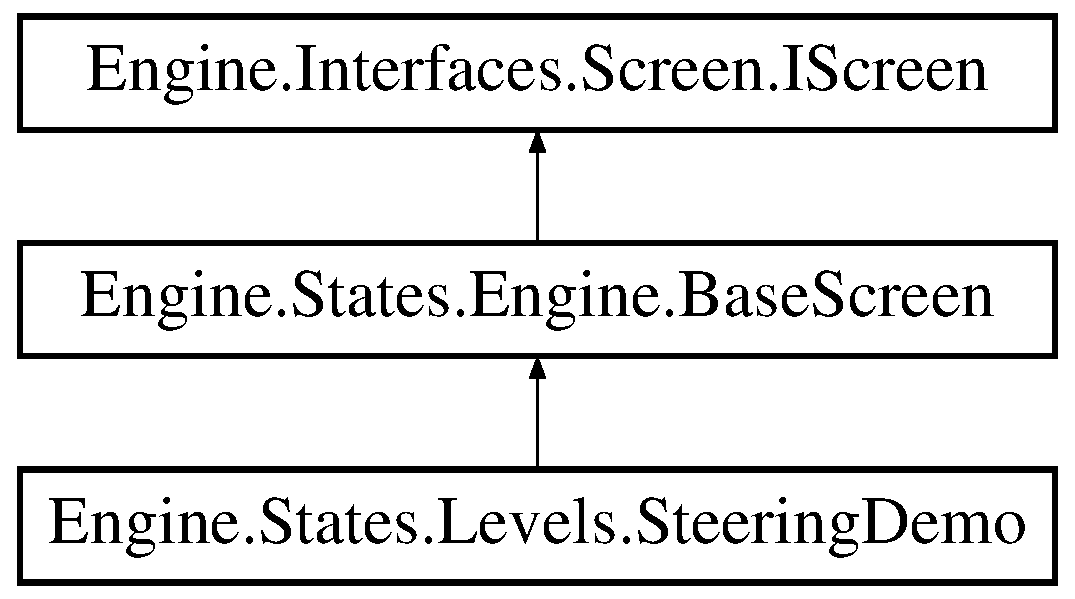
\includegraphics[height=3.000000cm]{d8/da5/a00570}
\end{center}
\end{figure}
\subsection*{Public Member Functions}
\begin{DoxyCompactItemize}
\item 
override void \hyperlink{a00570_a3ae8b73b4618e8c2635d3b8c24d70bcb}{Initialize} ()
\begin{DoxyCompactList}\small\item\em M\+E\+T\+H\+OD\+: Initialises the logic of the screen \end{DoxyCompactList}\item 
void \hyperlink{a00570_addcf72bee8c2ebbf4a7170c21fb49275}{On\+Key\+Pressed} (object source, \hyperlink{a00362}{Key\+Event\+Args} e)
\item 
override void \hyperlink{a00570_a32c772a646fe78f26a4e9f83ae327156}{Draw} (Sprite\+Batch sprite\+Batch)
\begin{DoxyCompactList}\small\item\em M\+E\+T\+H\+OD\+: Draws the content of the screen \end{DoxyCompactList}\item 
override void \hyperlink{a00570_a4210cc45e9038a007132fbafde08fa71}{Update} (Game\+Time game\+Time)
\begin{DoxyCompactList}\small\item\em M\+E\+T\+H\+OD\+: The update loop which is cycled through each frame \end{DoxyCompactList}\end{DoxyCompactItemize}
\subsection*{Additional Inherited Members}


\subsection{Member Function Documentation}
\mbox{\Hypertarget{a00570_a32c772a646fe78f26a4e9f83ae327156}\label{a00570_a32c772a646fe78f26a4e9f83ae327156}} 
\index{Engine\+::\+States\+::\+Levels\+::\+Steering\+Demo@{Engine\+::\+States\+::\+Levels\+::\+Steering\+Demo}!Draw@{Draw}}
\index{Draw@{Draw}!Engine\+::\+States\+::\+Levels\+::\+Steering\+Demo@{Engine\+::\+States\+::\+Levels\+::\+Steering\+Demo}}
\subsubsection{\texorpdfstring{Draw()}{Draw()}}
{\footnotesize\ttfamily override void Engine.\+States.\+Levels.\+Steering\+Demo.\+Draw (\begin{DoxyParamCaption}\item[{Sprite\+Batch}]{sprite\+Batch }\end{DoxyParamCaption})\hspace{0.3cm}{\ttfamily [inline]}, {\ttfamily [virtual]}}



M\+E\+T\+H\+OD\+: Draws the content of the screen 


\begin{DoxyParams}{Parameters}
{\em sprite\+Batch} & the Monogame Sprite\+Batch\\
\hline
\end{DoxyParams}


Reimplemented from \hyperlink{a00550_a200c31954effe5fc060118607155fb16}{Engine.\+States.\+Engine.\+Base\+Screen}.

\mbox{\Hypertarget{a00570_a3ae8b73b4618e8c2635d3b8c24d70bcb}\label{a00570_a3ae8b73b4618e8c2635d3b8c24d70bcb}} 
\index{Engine\+::\+States\+::\+Levels\+::\+Steering\+Demo@{Engine\+::\+States\+::\+Levels\+::\+Steering\+Demo}!Initialize@{Initialize}}
\index{Initialize@{Initialize}!Engine\+::\+States\+::\+Levels\+::\+Steering\+Demo@{Engine\+::\+States\+::\+Levels\+::\+Steering\+Demo}}
\subsubsection{\texorpdfstring{Initialize()}{Initialize()}}
{\footnotesize\ttfamily override void Engine.\+States.\+Levels.\+Steering\+Demo.\+Initialize (\begin{DoxyParamCaption}{ }\end{DoxyParamCaption})\hspace{0.3cm}{\ttfamily [inline]}, {\ttfamily [virtual]}}



M\+E\+T\+H\+OD\+: Initialises the logic of the screen 



Reimplemented from \hyperlink{a00550_af8fd6890abf865641e190578ef2e054c}{Engine.\+States.\+Engine.\+Base\+Screen}.

\mbox{\Hypertarget{a00570_addcf72bee8c2ebbf4a7170c21fb49275}\label{a00570_addcf72bee8c2ebbf4a7170c21fb49275}} 
\index{Engine\+::\+States\+::\+Levels\+::\+Steering\+Demo@{Engine\+::\+States\+::\+Levels\+::\+Steering\+Demo}!On\+Key\+Pressed@{On\+Key\+Pressed}}
\index{On\+Key\+Pressed@{On\+Key\+Pressed}!Engine\+::\+States\+::\+Levels\+::\+Steering\+Demo@{Engine\+::\+States\+::\+Levels\+::\+Steering\+Demo}}
\subsubsection{\texorpdfstring{On\+Key\+Pressed()}{OnKeyPressed()}}
{\footnotesize\ttfamily void Engine.\+States.\+Levels.\+Steering\+Demo.\+On\+Key\+Pressed (\begin{DoxyParamCaption}\item[{object}]{source,  }\item[{\hyperlink{a00362}{Key\+Event\+Args}}]{e }\end{DoxyParamCaption})\hspace{0.3cm}{\ttfamily [inline]}}

\mbox{\Hypertarget{a00570_a4210cc45e9038a007132fbafde08fa71}\label{a00570_a4210cc45e9038a007132fbafde08fa71}} 
\index{Engine\+::\+States\+::\+Levels\+::\+Steering\+Demo@{Engine\+::\+States\+::\+Levels\+::\+Steering\+Demo}!Update@{Update}}
\index{Update@{Update}!Engine\+::\+States\+::\+Levels\+::\+Steering\+Demo@{Engine\+::\+States\+::\+Levels\+::\+Steering\+Demo}}
\subsubsection{\texorpdfstring{Update()}{Update()}}
{\footnotesize\ttfamily override void Engine.\+States.\+Levels.\+Steering\+Demo.\+Update (\begin{DoxyParamCaption}\item[{Game\+Time}]{game\+Time }\end{DoxyParamCaption})\hspace{0.3cm}{\ttfamily [inline]}, {\ttfamily [virtual]}}



M\+E\+T\+H\+OD\+: The update loop which is cycled through each frame 


\begin{DoxyParams}{Parameters}
{\em game\+Time} & the Monogame Game\+Time property\\
\hline
\end{DoxyParams}


Reimplemented from \hyperlink{a00550_a098ece7d1e112475f6e880c3a672af64}{Engine.\+States.\+Engine.\+Base\+Screen}.



The documentation for this class was generated from the following file\+:\begin{DoxyCompactItemize}
\item 
\hyperlink{a00209}{Steering\+Demo.\+cs}\end{DoxyCompactItemize}

\hypertarget{a00342}{}\section{Engine.\+Entities.\+Steering.\+Steering\+Entity Class Reference}
\label{a00342}\index{Engine.\+Entities.\+Steering.\+Steering\+Entity@{Engine.\+Entities.\+Steering.\+Steering\+Entity}}
Inheritance diagram for Engine.\+Entities.\+Steering.\+Steering\+Entity\+:\begin{figure}[H]
\begin{center}
\leavevmode
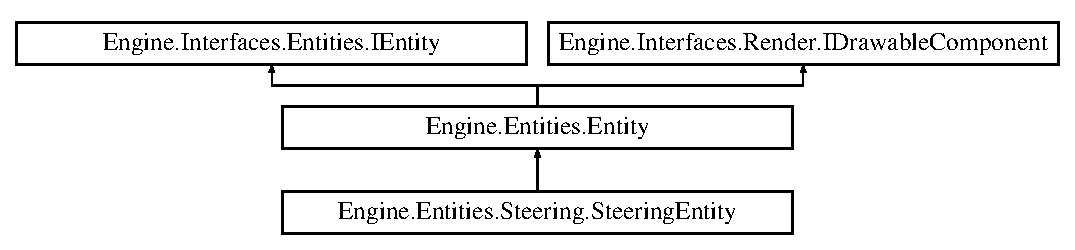
\includegraphics[height=2.916667cm]{d2/d45/a00342}
\end{center}
\end{figure}
\subsection*{Public Member Functions}
\begin{DoxyCompactItemize}
\item 
override void \hyperlink{a00342_a7b1e3df5320c999d2cf1cc3b97994401}{Initialize} (Vector2 Pos)
\begin{DoxyCompactList}\small\item\em M\+E\+T\+H\+OD\+: Initialises the basic properties of this entity, such as the mind \end{DoxyCompactList}\end{DoxyCompactItemize}
\subsection*{Additional Inherited Members}


\subsection{Member Function Documentation}
\mbox{\Hypertarget{a00342_a7b1e3df5320c999d2cf1cc3b97994401}\label{a00342_a7b1e3df5320c999d2cf1cc3b97994401}} 
\index{Engine\+::\+Entities\+::\+Steering\+::\+Steering\+Entity@{Engine\+::\+Entities\+::\+Steering\+::\+Steering\+Entity}!Initialize@{Initialize}}
\index{Initialize@{Initialize}!Engine\+::\+Entities\+::\+Steering\+::\+Steering\+Entity@{Engine\+::\+Entities\+::\+Steering\+::\+Steering\+Entity}}
\subsubsection{\texorpdfstring{Initialize()}{Initialize()}}
{\footnotesize\ttfamily override void Engine.\+Entities.\+Steering.\+Steering\+Entity.\+Initialize (\begin{DoxyParamCaption}\item[{Vector2}]{Pos }\end{DoxyParamCaption})\hspace{0.3cm}{\ttfamily [inline]}, {\ttfamily [virtual]}}



M\+E\+T\+H\+OD\+: Initialises the basic properties of this entity, such as the mind 


\begin{DoxyParams}{Parameters}
{\em Pos} & \\
\hline
\end{DoxyParams}
IF\+: The mind is not null, T\+H\+EN initialise the mind. 

Reimplemented from \hyperlink{a00314_aa1425aeeac379c5141e7560b84850b3d}{Engine.\+Entities.\+Entity}.



The documentation for this class was generated from the following file\+:\begin{DoxyCompactItemize}
\item 
\hyperlink{a00038}{Steering\+Entity.\+cs}\end{DoxyCompactItemize}

\hypertarget{a00346}{}\section{Engine.\+Entities.\+Steering.\+Steering\+Mind Class Reference}
\label{a00346}\index{Engine.\+Entities.\+Steering.\+Steering\+Mind@{Engine.\+Entities.\+Steering.\+Steering\+Mind}}
Inheritance diagram for Engine.\+Entities.\+Steering.\+Steering\+Mind\+:\begin{figure}[H]
\begin{center}
\leavevmode
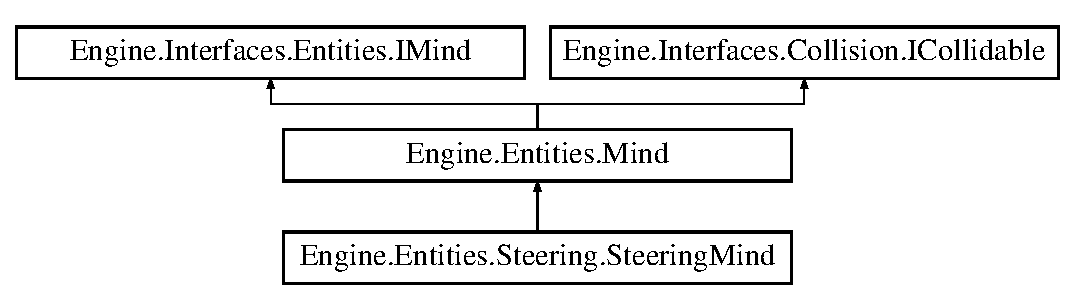
\includegraphics[height=3.000000cm]{d2/daf/a00346}
\end{center}
\end{figure}
\subsection*{Public Member Functions}
\begin{DoxyCompactItemize}
\item 
override void \hyperlink{a00346_a72922ee865087d504b1bca3fec35fb6e}{Initialize} (Vector2 \hyperlink{a00318_ad94b3975c0873fee06b5bd5a75bd38cd}{Position})
\begin{DoxyCompactList}\small\item\em M\+E\+T\+H\+OD\+: Initialises the basic properties of the mind when a texture has already been set \end{DoxyCompactList}\item 
void \hyperlink{a00346_a953d98dcd5ed2452a71e3658ecd5cf98}{Wander} ()
\item 
void \hyperlink{a00346_a232fba946737dac94731aff851985745}{flock} ()
\item 
void \hyperlink{a00346_a000c9f424dfdaedfb3ab00f8771ef859}{set\+Path} (List$<$ \hyperlink{a00414}{Node} $>$ path)
\item 
void \hyperlink{a00346_ab5caa6343f2e5d5d1854534ed919d018}{follow\+Way\+Points} ()
\item 
void \hyperlink{a00346_a593b91907bcd8d144942dd156ce7fc7e}{On\+Mouse\+Moved} (object sender, \hyperlink{a00374}{Mouse\+Event\+Args} k)
\item 
override void \hyperlink{a00346_a2e1f7ec281cfe2b7e8268a93bec59d4a}{Update} (Game\+Time game\+Time)
\begin{DoxyCompactList}\small\item\em M\+E\+T\+H\+OD\+: Update is called every frame and controls the main behaviour of the \hyperlink{a00318}{Mind}. \end{DoxyCompactList}\item 
Vector2 \hyperlink{a00346_a7c7017d89a91f07f479af5cc0ecc5eab}{flock\+Behaviour} (Vector2 v)
\item 
void \hyperlink{a00346_afb0d53f8cb93f437b89dbdc5ac0f71a2}{Seek} (Vector2 Target)
\item 
void \hyperlink{a00346_a882738a351da9a030468a018c69ee216}{Flee} (Vector2 Target)
\item 
void \hyperlink{a00346_a14fb4afcb6260502a8c545279ed6c8dc}{Pursue} (Vector2 Target, Vector2 Targets\+Velocity)
\item 
void \hyperlink{a00346_ac10a724f1df5a665fa88adbe97969d9c}{Evade} (Vector2 Target, Vector2 Targets\+Velocity)
\item 
void \hyperlink{a00346_a9e29641a665b426ba24b22282b5a4afb}{Arrival} (Vector2 Target, float radius)
\item 
Vector2 \hyperlink{a00346_a49d9a3d4beda2bfaffac447989b9c7b8}{calc\+Seperation} ()
\item 
Vector2 \hyperlink{a00346_a249ef5693985389b6c3e36bbc6a5b905}{calc\+Cohesion} ()
\item 
Vector2 \hyperlink{a00346_aeb7e79e42213d164fbf46bff97dc3b26}{calc\+Alignment} ()
\item 
void \hyperlink{a00346_ac9f9147dba78c35e082b00463696e846}{set\+Neighbourhood} (List$<$ \hyperlink{a00346}{Steering\+Mind} $>$ list)
\item 
Vector2 \hyperlink{a00346_a3006887440eba9edfd5e97bc56febca1}{Check\+Max} (Vector2 v, float max\+Value)
\item 
override void \hyperlink{a00346_a4834c17e78fd0bf82940ca0a4e8966f9}{On\+S\+A\+T\+Collision} (object sender, \hyperlink{a00350}{Collision\+Event\+Args} \hyperlink{a00318_ad89c9691d6b32053fe8ffcdeb68bdacf}{e})
\begin{DoxyCompactList}\small\item\em E\+V\+E\+NT\+: When S\+AT Collision returns true. \end{DoxyCompactList}\item 
Vector2 \hyperlink{a00346_a38152ad6c1dd536187718723061311e4}{get\+Velocity} ()
\item 
Vector2 \hyperlink{a00346_a5ba51a02c0ff7cebadee5c7b18eba5a7}{get\+Position} ()
\item 
Vector2 \hyperlink{a00346_a70f1b35eccd31d3efe3ec7266c77d7c5}{get\+Normal\+Pos} ()
\item 
Vector2 \hyperlink{a00346_a3193d5ceb8a7f78b21d4ff24977e442e}{get\+Normal\+Vel} ()
\item 
Vector2 \hyperlink{a00346_a7828d8105c471ce2e6e134344ad2e379}{get\+Normal\+Des\+Vel} ()
\item 
Vector2 \hyperlink{a00346_a32beb8852d356c29b1d1bf91cce908e5}{get\+Normal\+Steering} ()
\end{DoxyCompactItemize}
\subsection*{Data Fields}
\begin{DoxyCompactItemize}
\item 
Vector2 \hyperlink{a00346_a204d03e4db979c7fd987cd17c09cc15c}{steering\+Force}
\item 
\hyperlink{a00438}{I\+Entity} \hyperlink{a00346_ab7696a602bd19d445ee35f6df2572fcb}{current}
\end{DoxyCompactItemize}
\subsection*{Properties}
\begin{DoxyCompactItemize}
\item 
List$<$ \hyperlink{a00414}{Node} $>$ \hyperlink{a00346_a4b20dbb0da7a1f8b2f54c8141051f87f}{Pathway}\hspace{0.3cm}{\ttfamily  \mbox{[}get\mbox{]}}
\end{DoxyCompactItemize}
\subsection*{Additional Inherited Members}


\subsection{Member Function Documentation}
\mbox{\Hypertarget{a00346_a9e29641a665b426ba24b22282b5a4afb}\label{a00346_a9e29641a665b426ba24b22282b5a4afb}} 
\index{Engine\+::\+Entities\+::\+Steering\+::\+Steering\+Mind@{Engine\+::\+Entities\+::\+Steering\+::\+Steering\+Mind}!Arrival@{Arrival}}
\index{Arrival@{Arrival}!Engine\+::\+Entities\+::\+Steering\+::\+Steering\+Mind@{Engine\+::\+Entities\+::\+Steering\+::\+Steering\+Mind}}
\subsubsection{\texorpdfstring{Arrival()}{Arrival()}}
{\footnotesize\ttfamily void Engine.\+Entities.\+Steering.\+Steering\+Mind.\+Arrival (\begin{DoxyParamCaption}\item[{Vector2}]{Target,  }\item[{float}]{radius }\end{DoxyParamCaption})\hspace{0.3cm}{\ttfamily [inline]}}

\mbox{\Hypertarget{a00346_aeb7e79e42213d164fbf46bff97dc3b26}\label{a00346_aeb7e79e42213d164fbf46bff97dc3b26}} 
\index{Engine\+::\+Entities\+::\+Steering\+::\+Steering\+Mind@{Engine\+::\+Entities\+::\+Steering\+::\+Steering\+Mind}!calc\+Alignment@{calc\+Alignment}}
\index{calc\+Alignment@{calc\+Alignment}!Engine\+::\+Entities\+::\+Steering\+::\+Steering\+Mind@{Engine\+::\+Entities\+::\+Steering\+::\+Steering\+Mind}}
\subsubsection{\texorpdfstring{calc\+Alignment()}{calcAlignment()}}
{\footnotesize\ttfamily Vector2 Engine.\+Entities.\+Steering.\+Steering\+Mind.\+calc\+Alignment (\begin{DoxyParamCaption}{ }\end{DoxyParamCaption})\hspace{0.3cm}{\ttfamily [inline]}}





\begin{DoxyReturn}{Returns}

\end{DoxyReturn}
\mbox{\Hypertarget{a00346_a249ef5693985389b6c3e36bbc6a5b905}\label{a00346_a249ef5693985389b6c3e36bbc6a5b905}} 
\index{Engine\+::\+Entities\+::\+Steering\+::\+Steering\+Mind@{Engine\+::\+Entities\+::\+Steering\+::\+Steering\+Mind}!calc\+Cohesion@{calc\+Cohesion}}
\index{calc\+Cohesion@{calc\+Cohesion}!Engine\+::\+Entities\+::\+Steering\+::\+Steering\+Mind@{Engine\+::\+Entities\+::\+Steering\+::\+Steering\+Mind}}
\subsubsection{\texorpdfstring{calc\+Cohesion()}{calcCohesion()}}
{\footnotesize\ttfamily Vector2 Engine.\+Entities.\+Steering.\+Steering\+Mind.\+calc\+Cohesion (\begin{DoxyParamCaption}{ }\end{DoxyParamCaption})\hspace{0.3cm}{\ttfamily [inline]}}





\begin{DoxyReturn}{Returns}

\end{DoxyReturn}
\mbox{\Hypertarget{a00346_a49d9a3d4beda2bfaffac447989b9c7b8}\label{a00346_a49d9a3d4beda2bfaffac447989b9c7b8}} 
\index{Engine\+::\+Entities\+::\+Steering\+::\+Steering\+Mind@{Engine\+::\+Entities\+::\+Steering\+::\+Steering\+Mind}!calc\+Seperation@{calc\+Seperation}}
\index{calc\+Seperation@{calc\+Seperation}!Engine\+::\+Entities\+::\+Steering\+::\+Steering\+Mind@{Engine\+::\+Entities\+::\+Steering\+::\+Steering\+Mind}}
\subsubsection{\texorpdfstring{calc\+Seperation()}{calcSeperation()}}
{\footnotesize\ttfamily Vector2 Engine.\+Entities.\+Steering.\+Steering\+Mind.\+calc\+Seperation (\begin{DoxyParamCaption}{ }\end{DoxyParamCaption})\hspace{0.3cm}{\ttfamily [inline]}}





\begin{DoxyReturn}{Returns}

\end{DoxyReturn}
\mbox{\Hypertarget{a00346_a3006887440eba9edfd5e97bc56febca1}\label{a00346_a3006887440eba9edfd5e97bc56febca1}} 
\index{Engine\+::\+Entities\+::\+Steering\+::\+Steering\+Mind@{Engine\+::\+Entities\+::\+Steering\+::\+Steering\+Mind}!Check\+Max@{Check\+Max}}
\index{Check\+Max@{Check\+Max}!Engine\+::\+Entities\+::\+Steering\+::\+Steering\+Mind@{Engine\+::\+Entities\+::\+Steering\+::\+Steering\+Mind}}
\subsubsection{\texorpdfstring{Check\+Max()}{CheckMax()}}
{\footnotesize\ttfamily Vector2 Engine.\+Entities.\+Steering.\+Steering\+Mind.\+Check\+Max (\begin{DoxyParamCaption}\item[{Vector2}]{v,  }\item[{float}]{max\+Value }\end{DoxyParamCaption})\hspace{0.3cm}{\ttfamily [inline]}}

\mbox{\Hypertarget{a00346_ac10a724f1df5a665fa88adbe97969d9c}\label{a00346_ac10a724f1df5a665fa88adbe97969d9c}} 
\index{Engine\+::\+Entities\+::\+Steering\+::\+Steering\+Mind@{Engine\+::\+Entities\+::\+Steering\+::\+Steering\+Mind}!Evade@{Evade}}
\index{Evade@{Evade}!Engine\+::\+Entities\+::\+Steering\+::\+Steering\+Mind@{Engine\+::\+Entities\+::\+Steering\+::\+Steering\+Mind}}
\subsubsection{\texorpdfstring{Evade()}{Evade()}}
{\footnotesize\ttfamily void Engine.\+Entities.\+Steering.\+Steering\+Mind.\+Evade (\begin{DoxyParamCaption}\item[{Vector2}]{Target,  }\item[{Vector2}]{Targets\+Velocity }\end{DoxyParamCaption})\hspace{0.3cm}{\ttfamily [inline]}}






\begin{DoxyParams}{Parameters}
{\em Target} & \\
\hline
{\em Targets\+Velocity} & \\
\hline
\end{DoxyParams}
\mbox{\Hypertarget{a00346_a882738a351da9a030468a018c69ee216}\label{a00346_a882738a351da9a030468a018c69ee216}} 
\index{Engine\+::\+Entities\+::\+Steering\+::\+Steering\+Mind@{Engine\+::\+Entities\+::\+Steering\+::\+Steering\+Mind}!Flee@{Flee}}
\index{Flee@{Flee}!Engine\+::\+Entities\+::\+Steering\+::\+Steering\+Mind@{Engine\+::\+Entities\+::\+Steering\+::\+Steering\+Mind}}
\subsubsection{\texorpdfstring{Flee()}{Flee()}}
{\footnotesize\ttfamily void Engine.\+Entities.\+Steering.\+Steering\+Mind.\+Flee (\begin{DoxyParamCaption}\item[{Vector2}]{Target }\end{DoxyParamCaption})\hspace{0.3cm}{\ttfamily [inline]}}






\begin{DoxyParams}{Parameters}
{\em Target} & \\
\hline
\end{DoxyParams}
\mbox{\Hypertarget{a00346_a232fba946737dac94731aff851985745}\label{a00346_a232fba946737dac94731aff851985745}} 
\index{Engine\+::\+Entities\+::\+Steering\+::\+Steering\+Mind@{Engine\+::\+Entities\+::\+Steering\+::\+Steering\+Mind}!flock@{flock}}
\index{flock@{flock}!Engine\+::\+Entities\+::\+Steering\+::\+Steering\+Mind@{Engine\+::\+Entities\+::\+Steering\+::\+Steering\+Mind}}
\subsubsection{\texorpdfstring{flock()}{flock()}}
{\footnotesize\ttfamily void Engine.\+Entities.\+Steering.\+Steering\+Mind.\+flock (\begin{DoxyParamCaption}{ }\end{DoxyParamCaption})\hspace{0.3cm}{\ttfamily [inline]}}

\mbox{\Hypertarget{a00346_a7c7017d89a91f07f479af5cc0ecc5eab}\label{a00346_a7c7017d89a91f07f479af5cc0ecc5eab}} 
\index{Engine\+::\+Entities\+::\+Steering\+::\+Steering\+Mind@{Engine\+::\+Entities\+::\+Steering\+::\+Steering\+Mind}!flock\+Behaviour@{flock\+Behaviour}}
\index{flock\+Behaviour@{flock\+Behaviour}!Engine\+::\+Entities\+::\+Steering\+::\+Steering\+Mind@{Engine\+::\+Entities\+::\+Steering\+::\+Steering\+Mind}}
\subsubsection{\texorpdfstring{flock\+Behaviour()}{flockBehaviour()}}
{\footnotesize\ttfamily Vector2 Engine.\+Entities.\+Steering.\+Steering\+Mind.\+flock\+Behaviour (\begin{DoxyParamCaption}\item[{Vector2}]{v }\end{DoxyParamCaption})\hspace{0.3cm}{\ttfamily [inline]}}






\begin{DoxyParams}{Parameters}
{\em v} & \\
\hline
\end{DoxyParams}
\begin{DoxyReturn}{Returns}

\end{DoxyReturn}
\mbox{\Hypertarget{a00346_ab5caa6343f2e5d5d1854534ed919d018}\label{a00346_ab5caa6343f2e5d5d1854534ed919d018}} 
\index{Engine\+::\+Entities\+::\+Steering\+::\+Steering\+Mind@{Engine\+::\+Entities\+::\+Steering\+::\+Steering\+Mind}!follow\+Way\+Points@{follow\+Way\+Points}}
\index{follow\+Way\+Points@{follow\+Way\+Points}!Engine\+::\+Entities\+::\+Steering\+::\+Steering\+Mind@{Engine\+::\+Entities\+::\+Steering\+::\+Steering\+Mind}}
\subsubsection{\texorpdfstring{follow\+Way\+Points()}{followWayPoints()}}
{\footnotesize\ttfamily void Engine.\+Entities.\+Steering.\+Steering\+Mind.\+follow\+Way\+Points (\begin{DoxyParamCaption}{ }\end{DoxyParamCaption})\hspace{0.3cm}{\ttfamily [inline]}}

\mbox{\Hypertarget{a00346_a7828d8105c471ce2e6e134344ad2e379}\label{a00346_a7828d8105c471ce2e6e134344ad2e379}} 
\index{Engine\+::\+Entities\+::\+Steering\+::\+Steering\+Mind@{Engine\+::\+Entities\+::\+Steering\+::\+Steering\+Mind}!get\+Normal\+Des\+Vel@{get\+Normal\+Des\+Vel}}
\index{get\+Normal\+Des\+Vel@{get\+Normal\+Des\+Vel}!Engine\+::\+Entities\+::\+Steering\+::\+Steering\+Mind@{Engine\+::\+Entities\+::\+Steering\+::\+Steering\+Mind}}
\subsubsection{\texorpdfstring{get\+Normal\+Des\+Vel()}{getNormalDesVel()}}
{\footnotesize\ttfamily Vector2 Engine.\+Entities.\+Steering.\+Steering\+Mind.\+get\+Normal\+Des\+Vel (\begin{DoxyParamCaption}{ }\end{DoxyParamCaption})\hspace{0.3cm}{\ttfamily [inline]}}

\mbox{\Hypertarget{a00346_a70f1b35eccd31d3efe3ec7266c77d7c5}\label{a00346_a70f1b35eccd31d3efe3ec7266c77d7c5}} 
\index{Engine\+::\+Entities\+::\+Steering\+::\+Steering\+Mind@{Engine\+::\+Entities\+::\+Steering\+::\+Steering\+Mind}!get\+Normal\+Pos@{get\+Normal\+Pos}}
\index{get\+Normal\+Pos@{get\+Normal\+Pos}!Engine\+::\+Entities\+::\+Steering\+::\+Steering\+Mind@{Engine\+::\+Entities\+::\+Steering\+::\+Steering\+Mind}}
\subsubsection{\texorpdfstring{get\+Normal\+Pos()}{getNormalPos()}}
{\footnotesize\ttfamily Vector2 Engine.\+Entities.\+Steering.\+Steering\+Mind.\+get\+Normal\+Pos (\begin{DoxyParamCaption}{ }\end{DoxyParamCaption})\hspace{0.3cm}{\ttfamily [inline]}}

\mbox{\Hypertarget{a00346_a32beb8852d356c29b1d1bf91cce908e5}\label{a00346_a32beb8852d356c29b1d1bf91cce908e5}} 
\index{Engine\+::\+Entities\+::\+Steering\+::\+Steering\+Mind@{Engine\+::\+Entities\+::\+Steering\+::\+Steering\+Mind}!get\+Normal\+Steering@{get\+Normal\+Steering}}
\index{get\+Normal\+Steering@{get\+Normal\+Steering}!Engine\+::\+Entities\+::\+Steering\+::\+Steering\+Mind@{Engine\+::\+Entities\+::\+Steering\+::\+Steering\+Mind}}
\subsubsection{\texorpdfstring{get\+Normal\+Steering()}{getNormalSteering()}}
{\footnotesize\ttfamily Vector2 Engine.\+Entities.\+Steering.\+Steering\+Mind.\+get\+Normal\+Steering (\begin{DoxyParamCaption}{ }\end{DoxyParamCaption})\hspace{0.3cm}{\ttfamily [inline]}}

\mbox{\Hypertarget{a00346_a3193d5ceb8a7f78b21d4ff24977e442e}\label{a00346_a3193d5ceb8a7f78b21d4ff24977e442e}} 
\index{Engine\+::\+Entities\+::\+Steering\+::\+Steering\+Mind@{Engine\+::\+Entities\+::\+Steering\+::\+Steering\+Mind}!get\+Normal\+Vel@{get\+Normal\+Vel}}
\index{get\+Normal\+Vel@{get\+Normal\+Vel}!Engine\+::\+Entities\+::\+Steering\+::\+Steering\+Mind@{Engine\+::\+Entities\+::\+Steering\+::\+Steering\+Mind}}
\subsubsection{\texorpdfstring{get\+Normal\+Vel()}{getNormalVel()}}
{\footnotesize\ttfamily Vector2 Engine.\+Entities.\+Steering.\+Steering\+Mind.\+get\+Normal\+Vel (\begin{DoxyParamCaption}{ }\end{DoxyParamCaption})\hspace{0.3cm}{\ttfamily [inline]}}

\mbox{\Hypertarget{a00346_a5ba51a02c0ff7cebadee5c7b18eba5a7}\label{a00346_a5ba51a02c0ff7cebadee5c7b18eba5a7}} 
\index{Engine\+::\+Entities\+::\+Steering\+::\+Steering\+Mind@{Engine\+::\+Entities\+::\+Steering\+::\+Steering\+Mind}!get\+Position@{get\+Position}}
\index{get\+Position@{get\+Position}!Engine\+::\+Entities\+::\+Steering\+::\+Steering\+Mind@{Engine\+::\+Entities\+::\+Steering\+::\+Steering\+Mind}}
\subsubsection{\texorpdfstring{get\+Position()}{getPosition()}}
{\footnotesize\ttfamily Vector2 Engine.\+Entities.\+Steering.\+Steering\+Mind.\+get\+Position (\begin{DoxyParamCaption}{ }\end{DoxyParamCaption})\hspace{0.3cm}{\ttfamily [inline]}}

\mbox{\Hypertarget{a00346_a38152ad6c1dd536187718723061311e4}\label{a00346_a38152ad6c1dd536187718723061311e4}} 
\index{Engine\+::\+Entities\+::\+Steering\+::\+Steering\+Mind@{Engine\+::\+Entities\+::\+Steering\+::\+Steering\+Mind}!get\+Velocity@{get\+Velocity}}
\index{get\+Velocity@{get\+Velocity}!Engine\+::\+Entities\+::\+Steering\+::\+Steering\+Mind@{Engine\+::\+Entities\+::\+Steering\+::\+Steering\+Mind}}
\subsubsection{\texorpdfstring{get\+Velocity()}{getVelocity()}}
{\footnotesize\ttfamily Vector2 Engine.\+Entities.\+Steering.\+Steering\+Mind.\+get\+Velocity (\begin{DoxyParamCaption}{ }\end{DoxyParamCaption})\hspace{0.3cm}{\ttfamily [inline]}}

\mbox{\Hypertarget{a00346_a72922ee865087d504b1bca3fec35fb6e}\label{a00346_a72922ee865087d504b1bca3fec35fb6e}} 
\index{Engine\+::\+Entities\+::\+Steering\+::\+Steering\+Mind@{Engine\+::\+Entities\+::\+Steering\+::\+Steering\+Mind}!Initialize@{Initialize}}
\index{Initialize@{Initialize}!Engine\+::\+Entities\+::\+Steering\+::\+Steering\+Mind@{Engine\+::\+Entities\+::\+Steering\+::\+Steering\+Mind}}
\subsubsection{\texorpdfstring{Initialize()}{Initialize()}}
{\footnotesize\ttfamily override void Engine.\+Entities.\+Steering.\+Steering\+Mind.\+Initialize (\begin{DoxyParamCaption}\item[{Vector2}]{Position }\end{DoxyParamCaption})\hspace{0.3cm}{\ttfamily [inline]}, {\ttfamily [virtual]}}



M\+E\+T\+H\+OD\+: Initialises the basic properties of the mind when a texture has already been set 


\begin{DoxyParams}{Parameters}
{\em Position} & \\
\hline
\end{DoxyParams}
H\+A\+N\+D\+L\+ER\+: Add handler for S\+AT collision

S\+ET\+: T\+He unique ID for this mind

IF\+: Texture path is not null

C\+A\+LL\+: Set texture

S\+ET\+: position and visibility of \hyperlink{a00314}{Entity} controlled by this mind.

S\+ET\+: The position of this mind and whether it is active. 

Reimplemented from \hyperlink{a00318_a353d7d2bb1035aefebf0ae3e3f1d1488}{Engine.\+Entities.\+Mind}.

\mbox{\Hypertarget{a00346_a593b91907bcd8d144942dd156ce7fc7e}\label{a00346_a593b91907bcd8d144942dd156ce7fc7e}} 
\index{Engine\+::\+Entities\+::\+Steering\+::\+Steering\+Mind@{Engine\+::\+Entities\+::\+Steering\+::\+Steering\+Mind}!On\+Mouse\+Moved@{On\+Mouse\+Moved}}
\index{On\+Mouse\+Moved@{On\+Mouse\+Moved}!Engine\+::\+Entities\+::\+Steering\+::\+Steering\+Mind@{Engine\+::\+Entities\+::\+Steering\+::\+Steering\+Mind}}
\subsubsection{\texorpdfstring{On\+Mouse\+Moved()}{OnMouseMoved()}}
{\footnotesize\ttfamily void Engine.\+Entities.\+Steering.\+Steering\+Mind.\+On\+Mouse\+Moved (\begin{DoxyParamCaption}\item[{object}]{sender,  }\item[{\hyperlink{a00374}{Mouse\+Event\+Args}}]{k }\end{DoxyParamCaption})\hspace{0.3cm}{\ttfamily [inline]}}

\mbox{\Hypertarget{a00346_a4834c17e78fd0bf82940ca0a4e8966f9}\label{a00346_a4834c17e78fd0bf82940ca0a4e8966f9}} 
\index{Engine\+::\+Entities\+::\+Steering\+::\+Steering\+Mind@{Engine\+::\+Entities\+::\+Steering\+::\+Steering\+Mind}!On\+S\+A\+T\+Collision@{On\+S\+A\+T\+Collision}}
\index{On\+S\+A\+T\+Collision@{On\+S\+A\+T\+Collision}!Engine\+::\+Entities\+::\+Steering\+::\+Steering\+Mind@{Engine\+::\+Entities\+::\+Steering\+::\+Steering\+Mind}}
\subsubsection{\texorpdfstring{On\+S\+A\+T\+Collision()}{OnSATCollision()}}
{\footnotesize\ttfamily override void Engine.\+Entities.\+Steering.\+Steering\+Mind.\+On\+S\+A\+T\+Collision (\begin{DoxyParamCaption}\item[{object}]{sender,  }\item[{\hyperlink{a00350}{Collision\+Event\+Args}}]{e }\end{DoxyParamCaption})\hspace{0.3cm}{\ttfamily [inline]}, {\ttfamily [virtual]}}



E\+V\+E\+NT\+: When S\+AT Collision returns true. 


\begin{DoxyParams}{Parameters}
{\em sender} & \\
\hline
{\em e} & \\
\hline
\end{DoxyParams}
IF\+: This mind is object A, Apply Impulse to simulate physics

E\+L\+SE IF\+: this mind is object B, apply impulse in opposite direction 

Reimplemented from \hyperlink{a00318_ac278d4358d794426251d1b87b6aa7b82}{Engine.\+Entities.\+Mind}.

\mbox{\Hypertarget{a00346_a14fb4afcb6260502a8c545279ed6c8dc}\label{a00346_a14fb4afcb6260502a8c545279ed6c8dc}} 
\index{Engine\+::\+Entities\+::\+Steering\+::\+Steering\+Mind@{Engine\+::\+Entities\+::\+Steering\+::\+Steering\+Mind}!Pursue@{Pursue}}
\index{Pursue@{Pursue}!Engine\+::\+Entities\+::\+Steering\+::\+Steering\+Mind@{Engine\+::\+Entities\+::\+Steering\+::\+Steering\+Mind}}
\subsubsection{\texorpdfstring{Pursue()}{Pursue()}}
{\footnotesize\ttfamily void Engine.\+Entities.\+Steering.\+Steering\+Mind.\+Pursue (\begin{DoxyParamCaption}\item[{Vector2}]{Target,  }\item[{Vector2}]{Targets\+Velocity }\end{DoxyParamCaption})\hspace{0.3cm}{\ttfamily [inline]}}






\begin{DoxyParams}{Parameters}
{\em Target} & \\
\hline
{\em Targets\+Velocity} & \\
\hline
\end{DoxyParams}
\mbox{\Hypertarget{a00346_afb0d53f8cb93f437b89dbdc5ac0f71a2}\label{a00346_afb0d53f8cb93f437b89dbdc5ac0f71a2}} 
\index{Engine\+::\+Entities\+::\+Steering\+::\+Steering\+Mind@{Engine\+::\+Entities\+::\+Steering\+::\+Steering\+Mind}!Seek@{Seek}}
\index{Seek@{Seek}!Engine\+::\+Entities\+::\+Steering\+::\+Steering\+Mind@{Engine\+::\+Entities\+::\+Steering\+::\+Steering\+Mind}}
\subsubsection{\texorpdfstring{Seek()}{Seek()}}
{\footnotesize\ttfamily void Engine.\+Entities.\+Steering.\+Steering\+Mind.\+Seek (\begin{DoxyParamCaption}\item[{Vector2}]{Target }\end{DoxyParamCaption})\hspace{0.3cm}{\ttfamily [inline]}}






\begin{DoxyParams}{Parameters}
{\em Target} & \\
\hline
\end{DoxyParams}
\mbox{\Hypertarget{a00346_ac9f9147dba78c35e082b00463696e846}\label{a00346_ac9f9147dba78c35e082b00463696e846}} 
\index{Engine\+::\+Entities\+::\+Steering\+::\+Steering\+Mind@{Engine\+::\+Entities\+::\+Steering\+::\+Steering\+Mind}!set\+Neighbourhood@{set\+Neighbourhood}}
\index{set\+Neighbourhood@{set\+Neighbourhood}!Engine\+::\+Entities\+::\+Steering\+::\+Steering\+Mind@{Engine\+::\+Entities\+::\+Steering\+::\+Steering\+Mind}}
\subsubsection{\texorpdfstring{set\+Neighbourhood()}{setNeighbourhood()}}
{\footnotesize\ttfamily void Engine.\+Entities.\+Steering.\+Steering\+Mind.\+set\+Neighbourhood (\begin{DoxyParamCaption}\item[{List$<$ \hyperlink{a00346}{Steering\+Mind} $>$}]{list }\end{DoxyParamCaption})\hspace{0.3cm}{\ttfamily [inline]}}

\mbox{\Hypertarget{a00346_a000c9f424dfdaedfb3ab00f8771ef859}\label{a00346_a000c9f424dfdaedfb3ab00f8771ef859}} 
\index{Engine\+::\+Entities\+::\+Steering\+::\+Steering\+Mind@{Engine\+::\+Entities\+::\+Steering\+::\+Steering\+Mind}!set\+Path@{set\+Path}}
\index{set\+Path@{set\+Path}!Engine\+::\+Entities\+::\+Steering\+::\+Steering\+Mind@{Engine\+::\+Entities\+::\+Steering\+::\+Steering\+Mind}}
\subsubsection{\texorpdfstring{set\+Path()}{setPath()}}
{\footnotesize\ttfamily void Engine.\+Entities.\+Steering.\+Steering\+Mind.\+set\+Path (\begin{DoxyParamCaption}\item[{List$<$ \hyperlink{a00414}{Node} $>$}]{path }\end{DoxyParamCaption})\hspace{0.3cm}{\ttfamily [inline]}}

\mbox{\Hypertarget{a00346_a2e1f7ec281cfe2b7e8268a93bec59d4a}\label{a00346_a2e1f7ec281cfe2b7e8268a93bec59d4a}} 
\index{Engine\+::\+Entities\+::\+Steering\+::\+Steering\+Mind@{Engine\+::\+Entities\+::\+Steering\+::\+Steering\+Mind}!Update@{Update}}
\index{Update@{Update}!Engine\+::\+Entities\+::\+Steering\+::\+Steering\+Mind@{Engine\+::\+Entities\+::\+Steering\+::\+Steering\+Mind}}
\subsubsection{\texorpdfstring{Update()}{Update()}}
{\footnotesize\ttfamily override void Engine.\+Entities.\+Steering.\+Steering\+Mind.\+Update (\begin{DoxyParamCaption}\item[{Game\+Time}]{game\+Time }\end{DoxyParamCaption})\hspace{0.3cm}{\ttfamily [inline]}, {\ttfamily [virtual]}}



M\+E\+T\+H\+OD\+: Update is called every frame and controls the main behaviour of the \hyperlink{a00318}{Mind}. 


\begin{DoxyParams}{Parameters}
{\em game\+Time} & \\
\hline
\end{DoxyParams}
S\+ET\+: Position of controlled entity

IF\+: \hyperlink{a00318}{Mind} is no longer active

S\+ET\+: entity to not be drawn

C\+A\+LL\+: Method to simulate physical movement 

Reimplemented from \hyperlink{a00318_adec6999d87accf7371de1536eac2541b}{Engine.\+Entities.\+Mind}.

\mbox{\Hypertarget{a00346_a953d98dcd5ed2452a71e3658ecd5cf98}\label{a00346_a953d98dcd5ed2452a71e3658ecd5cf98}} 
\index{Engine\+::\+Entities\+::\+Steering\+::\+Steering\+Mind@{Engine\+::\+Entities\+::\+Steering\+::\+Steering\+Mind}!Wander@{Wander}}
\index{Wander@{Wander}!Engine\+::\+Entities\+::\+Steering\+::\+Steering\+Mind@{Engine\+::\+Entities\+::\+Steering\+::\+Steering\+Mind}}
\subsubsection{\texorpdfstring{Wander()}{Wander()}}
{\footnotesize\ttfamily void Engine.\+Entities.\+Steering.\+Steering\+Mind.\+Wander (\begin{DoxyParamCaption}{ }\end{DoxyParamCaption})\hspace{0.3cm}{\ttfamily [inline]}}



\subsection{Field Documentation}
\mbox{\Hypertarget{a00346_ab7696a602bd19d445ee35f6df2572fcb}\label{a00346_ab7696a602bd19d445ee35f6df2572fcb}} 
\index{Engine\+::\+Entities\+::\+Steering\+::\+Steering\+Mind@{Engine\+::\+Entities\+::\+Steering\+::\+Steering\+Mind}!current@{current}}
\index{current@{current}!Engine\+::\+Entities\+::\+Steering\+::\+Steering\+Mind@{Engine\+::\+Entities\+::\+Steering\+::\+Steering\+Mind}}
\subsubsection{\texorpdfstring{current}{current}}
{\footnotesize\ttfamily \hyperlink{a00438}{I\+Entity} Engine.\+Entities.\+Steering.\+Steering\+Mind.\+current}

\mbox{\Hypertarget{a00346_a204d03e4db979c7fd987cd17c09cc15c}\label{a00346_a204d03e4db979c7fd987cd17c09cc15c}} 
\index{Engine\+::\+Entities\+::\+Steering\+::\+Steering\+Mind@{Engine\+::\+Entities\+::\+Steering\+::\+Steering\+Mind}!steering\+Force@{steering\+Force}}
\index{steering\+Force@{steering\+Force}!Engine\+::\+Entities\+::\+Steering\+::\+Steering\+Mind@{Engine\+::\+Entities\+::\+Steering\+::\+Steering\+Mind}}
\subsubsection{\texorpdfstring{steering\+Force}{steeringForce}}
{\footnotesize\ttfamily Vector2 Engine.\+Entities.\+Steering.\+Steering\+Mind.\+steering\+Force}



\subsection{Property Documentation}
\mbox{\Hypertarget{a00346_a4b20dbb0da7a1f8b2f54c8141051f87f}\label{a00346_a4b20dbb0da7a1f8b2f54c8141051f87f}} 
\index{Engine\+::\+Entities\+::\+Steering\+::\+Steering\+Mind@{Engine\+::\+Entities\+::\+Steering\+::\+Steering\+Mind}!Pathway@{Pathway}}
\index{Pathway@{Pathway}!Engine\+::\+Entities\+::\+Steering\+::\+Steering\+Mind@{Engine\+::\+Entities\+::\+Steering\+::\+Steering\+Mind}}
\subsubsection{\texorpdfstring{Pathway}{Pathway}}
{\footnotesize\ttfamily List$<$\hyperlink{a00414}{Node}$>$ Engine.\+Entities.\+Steering.\+Steering\+Mind.\+Pathway\hspace{0.3cm}{\ttfamily [get]}}



The documentation for this class was generated from the following file\+:\begin{DoxyCompactItemize}
\item 
\hyperlink{a00041}{Steering\+Mind.\+cs}\end{DoxyCompactItemize}

\hypertarget{a00330}{}\section{Engine.\+Entities.\+Platformer.\+Test\+Entity Class Reference}
\label{a00330}\index{Engine.\+Entities.\+Platformer.\+Test\+Entity@{Engine.\+Entities.\+Platformer.\+Test\+Entity}}


C\+L\+A\+SS\+: A Test \hyperlink{a00314}{Entity} used for various demos.  


Inheritance diagram for Engine.\+Entities.\+Platformer.\+Test\+Entity\+:\begin{figure}[H]
\begin{center}
\leavevmode
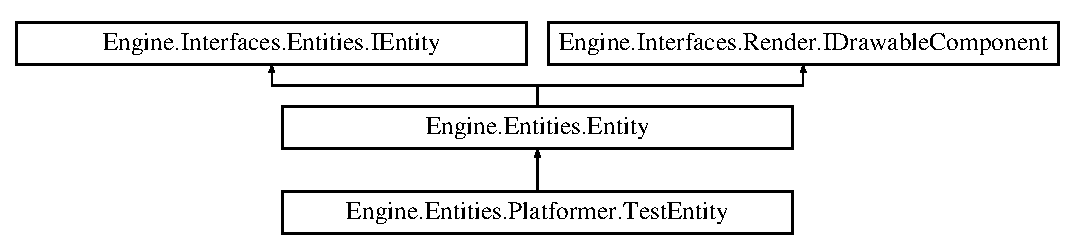
\includegraphics[height=2.916667cm]{dd/dbb/a00330}
\end{center}
\end{figure}
\subsection*{Public Member Functions}
\begin{DoxyCompactItemize}
\item 
override void \hyperlink{a00330_ad4122c4f38d98746a67532d0a6836da5}{Initialize} (Vector2 Pos)
\begin{DoxyCompactList}\small\item\em M\+E\+T\+H\+OD\+: Initialise the basic properties of the entity. \end{DoxyCompactList}\end{DoxyCompactItemize}
\subsection*{Additional Inherited Members}


\subsection{Detailed Description}
C\+L\+A\+SS\+: A Test \hyperlink{a00314}{Entity} used for various demos. 



\subsection{Member Function Documentation}
\mbox{\Hypertarget{a00330_ad4122c4f38d98746a67532d0a6836da5}\label{a00330_ad4122c4f38d98746a67532d0a6836da5}} 
\index{Engine\+::\+Entities\+::\+Platformer\+::\+Test\+Entity@{Engine\+::\+Entities\+::\+Platformer\+::\+Test\+Entity}!Initialize@{Initialize}}
\index{Initialize@{Initialize}!Engine\+::\+Entities\+::\+Platformer\+::\+Test\+Entity@{Engine\+::\+Entities\+::\+Platformer\+::\+Test\+Entity}}
\subsubsection{\texorpdfstring{Initialize()}{Initialize()}}
{\footnotesize\ttfamily override void Engine.\+Entities.\+Platformer.\+Test\+Entity.\+Initialize (\begin{DoxyParamCaption}\item[{Vector2}]{Pos }\end{DoxyParamCaption})\hspace{0.3cm}{\ttfamily [inline]}, {\ttfamily [virtual]}}



M\+E\+T\+H\+OD\+: Initialise the basic properties of the entity. 


\begin{DoxyParams}{Parameters}
{\em Pos} & \\
\hline
\end{DoxyParams}
S\+ET\+: the mind controlling this entity

C\+A\+LL\+: The initialise of the abstract entity class.

S\+ET\+: The name of this entity. 

Reimplemented from \hyperlink{a00314_aa1425aeeac379c5141e7560b84850b3d}{Engine.\+Entities.\+Entity}.



The documentation for this class was generated from the following file\+:\begin{DoxyCompactItemize}
\item 
\hyperlink{a00029}{Test\+Entity.\+cs}\end{DoxyCompactItemize}

\hypertarget{a00334}{}\section{Engine.\+Entities.\+Platformer.\+Test\+Mind Class Reference}
\label{a00334}\index{Engine.\+Entities.\+Platformer.\+Test\+Mind@{Engine.\+Entities.\+Platformer.\+Test\+Mind}}


C\+L\+A\+SS\+: A test mind to control a test entity for demos.  


Inheritance diagram for Engine.\+Entities.\+Platformer.\+Test\+Mind\+:\begin{figure}[H]
\begin{center}
\leavevmode
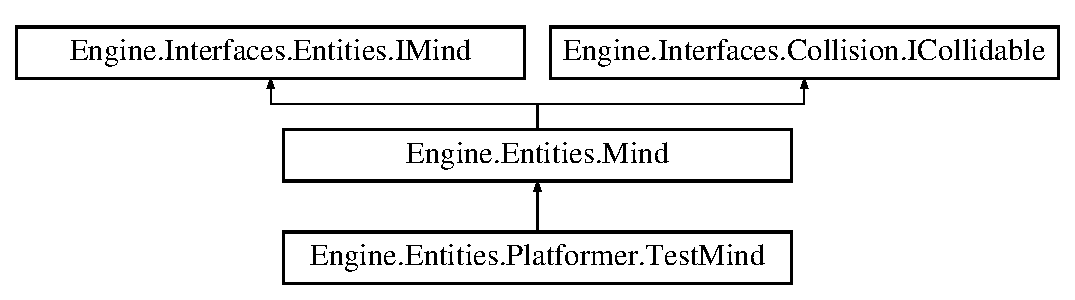
\includegraphics[height=3.000000cm]{da/d75/a00334}
\end{center}
\end{figure}
\subsection*{Public Member Functions}
\begin{DoxyCompactItemize}
\item 
override void \hyperlink{a00334_ae94a647a0b9c6f1d99abb61e36612ba7}{Initialize} (Vector2 \hyperlink{a00318_ad94b3975c0873fee06b5bd5a75bd38cd}{Position})
\begin{DoxyCompactList}\small\item\em M\+E\+T\+H\+OD\+: Initialises the basic properties of this mind. \end{DoxyCompactList}\item 
override void \hyperlink{a00334_a1817f5df935d637c737d510e39fd251f}{Update} (Game\+Time game\+Time)
\begin{DoxyCompactList}\small\item\em M\+E\+T\+H\+OD\+: The update method which is called and ran through every frame. \end{DoxyCompactList}\end{DoxyCompactItemize}
\subsection*{Additional Inherited Members}


\subsection{Detailed Description}
C\+L\+A\+SS\+: A test mind to control a test entity for demos. 



\subsection{Member Function Documentation}
\mbox{\Hypertarget{a00334_ae94a647a0b9c6f1d99abb61e36612ba7}\label{a00334_ae94a647a0b9c6f1d99abb61e36612ba7}} 
\index{Engine\+::\+Entities\+::\+Platformer\+::\+Test\+Mind@{Engine\+::\+Entities\+::\+Platformer\+::\+Test\+Mind}!Initialize@{Initialize}}
\index{Initialize@{Initialize}!Engine\+::\+Entities\+::\+Platformer\+::\+Test\+Mind@{Engine\+::\+Entities\+::\+Platformer\+::\+Test\+Mind}}
\subsubsection{\texorpdfstring{Initialize()}{Initialize()}}
{\footnotesize\ttfamily override void Engine.\+Entities.\+Platformer.\+Test\+Mind.\+Initialize (\begin{DoxyParamCaption}\item[{Vector2}]{Position }\end{DoxyParamCaption})\hspace{0.3cm}{\ttfamily [inline]}, {\ttfamily [virtual]}}



M\+E\+T\+H\+OD\+: Initialises the basic properties of this mind. 


\begin{DoxyParams}{Parameters}
{\em Position} & \\
\hline
\end{DoxyParams}
S\+ET\+: The texture of the entity this mind controls.

S\+ET\+: The basic physics properties

A\+DD\+: Hitboxes for the entity

C\+A\+LL\+: The initialise of the abstract mind class 

Reimplemented from \hyperlink{a00318_a353d7d2bb1035aefebf0ae3e3f1d1488}{Engine.\+Entities.\+Mind}.

\mbox{\Hypertarget{a00334_a1817f5df935d637c737d510e39fd251f}\label{a00334_a1817f5df935d637c737d510e39fd251f}} 
\index{Engine\+::\+Entities\+::\+Platformer\+::\+Test\+Mind@{Engine\+::\+Entities\+::\+Platformer\+::\+Test\+Mind}!Update@{Update}}
\index{Update@{Update}!Engine\+::\+Entities\+::\+Platformer\+::\+Test\+Mind@{Engine\+::\+Entities\+::\+Platformer\+::\+Test\+Mind}}
\subsubsection{\texorpdfstring{Update()}{Update()}}
{\footnotesize\ttfamily override void Engine.\+Entities.\+Platformer.\+Test\+Mind.\+Update (\begin{DoxyParamCaption}\item[{Game\+Time}]{game\+Time }\end{DoxyParamCaption})\hspace{0.3cm}{\ttfamily [inline]}, {\ttfamily [virtual]}}



M\+E\+T\+H\+OD\+: The update method which is called and ran through every frame. 


\begin{DoxyParams}{Parameters}
{\em game\+Time} & \\
\hline
\end{DoxyParams}
C\+A\+LL\+: The update physics method to simulate movement

C\+A\+LL\+: The update of the abstract class mind. 

Reimplemented from \hyperlink{a00318_adec6999d87accf7371de1536eac2541b}{Engine.\+Entities.\+Mind}.



The documentation for this class was generated from the following file\+:\begin{DoxyCompactItemize}
\item 
\hyperlink{a00032}{Test\+Mind.\+cs}\end{DoxyCompactItemize}

\chapter{File Documentation}
\hypertarget{a00155}{}\section{A\+A\+B\+B.\+cs File Reference}
\label{a00155}\index{A\+A\+B\+B.\+cs@{A\+A\+B\+B.\+cs}}
\subsection*{Data Structures}
\begin{DoxyCompactItemize}
\item 
class {\bfseries Engine.\+Managers.\+Collision.\+A\+A\+BB}
\end{DoxyCompactItemize}
\subsection*{Namespaces}
\begin{DoxyCompactItemize}
\item 
namespace \hyperlink{a00268}{Engine.\+Managers.\+Collision}
\end{DoxyCompactItemize}
\subsection*{Enumerations}
\begin{DoxyCompactItemize}
\item 
enum \hyperlink{a00268_addb954cde1b34937cfd0a187a154c8af}{Engine.\+Managers.\+Collision.\+Collision\+Side} \{ \newline
\hyperlink{a00268_addb954cde1b34937cfd0a187a154c8afa811882fecd5c7618d7099ebbd39ea254}{Engine.\+Managers.\+Collision.\+Collision\+Side.\+left}, 
\hyperlink{a00268_addb954cde1b34937cfd0a187a154c8afa7c4f29407893c334a6cb7a87bf045c0d}{Engine.\+Managers.\+Collision.\+Collision\+Side.\+right}, 
\hyperlink{a00268_addb954cde1b34937cfd0a187a154c8afab28354b543375bfa94dabaeda722927f}{Engine.\+Managers.\+Collision.\+Collision\+Side.\+top}, 
\hyperlink{a00268_addb954cde1b34937cfd0a187a154c8afa71f262d796bed1ab30e8a2d5a8ddee6f}{Engine.\+Managers.\+Collision.\+Collision\+Side.\+bottom}, 
\newline
\hyperlink{a00268_addb954cde1b34937cfd0a187a154c8afa334c4a4c42fdb79d7ebc3e73b517e6f8}{Engine.\+Managers.\+Collision.\+Collision\+Side.\+none}
 \}\begin{DoxyCompactList}\small\item\em C\+L\+A\+SS\+: A collision class used to calculate whether two axis aligned bounding boxes are intersecting or not. If they are intersecting this class can return true and state which side is intersecting and by how much. \end{DoxyCompactList}
\end{DoxyCompactItemize}

\hypertarget{a00002}{}\section{Animation\+Manager.\+cs File Reference}
\label{a00002}\index{Animation\+Manager.\+cs@{Animation\+Manager.\+cs}}
\subsection*{Data Structures}
\begin{DoxyCompactItemize}
\item 
class \hyperlink{a00298}{Engine.\+Managers.\+Animation\+Manager}
\end{DoxyCompactItemize}
\subsection*{Namespaces}
\begin{DoxyCompactItemize}
\item 
namespace \hyperlink{a00239}{Engine.\+Managers}
\end{DoxyCompactItemize}

\hypertarget{a00203}{}\section{A\+Star\+Demo.\+cs File Reference}
\label{a00203}\index{A\+Star\+Demo.\+cs@{A\+Star\+Demo.\+cs}}
\subsection*{Data Structures}
\begin{DoxyCompactItemize}
\item 
class \hyperlink{a00562}{Engine.\+States.\+Levels.\+A\+Star\+Demo}
\end{DoxyCompactItemize}
\subsection*{Namespaces}
\begin{DoxyCompactItemize}
\item 
namespace \hyperlink{a00279}{Engine.\+States.\+Levels}
\end{DoxyCompactItemize}

\hypertarget{a00080}{}\section{A\+Star\+Grid\+Search.\+cs File Reference}
\label{a00080}\index{A\+Star\+Grid\+Search.\+cs@{A\+Star\+Grid\+Search.\+cs}}
\subsection*{Data Structures}
\begin{DoxyCompactItemize}
\item 
class \hyperlink{a00398}{Engine.\+Grid.\+A\+Star\+Grid\+Search}
\end{DoxyCompactItemize}
\subsection*{Namespaces}
\begin{DoxyCompactItemize}
\item 
namespace \hyperlink{a00251}{Engine.\+Grid}
\end{DoxyCompactItemize}

\hypertarget{a00083}{}\section{A\+Star\+Node.\+cs File Reference}
\label{a00083}\index{A\+Star\+Node.\+cs@{A\+Star\+Node.\+cs}}
\subsection*{Data Structures}
\begin{DoxyCompactItemize}
\item 
class \hyperlink{a00402}{Engine.\+Grid.\+A\+Star\+Node}
\end{DoxyCompactItemize}
\subsection*{Namespaces}
\begin{DoxyCompactItemize}
\item 
namespace \hyperlink{a00251}{Engine.\+Grid}
\end{DoxyCompactItemize}

\hypertarget{a00014}{}\section{Astar\+Path.\+cs File Reference}
\label{a00014}\index{Astar\+Path.\+cs@{Astar\+Path.\+cs}}
\subsection*{Data Structures}
\begin{DoxyCompactItemize}
\item 
class \hyperlink{a00310}{Engine.\+Managers.\+A\+Star.\+Astar\+Path}
\end{DoxyCompactItemize}
\subsection*{Namespaces}
\begin{DoxyCompactItemize}
\item 
namespace \hyperlink{a00241}{Engine.\+Managers.\+A\+Star}
\end{DoxyCompactItemize}

\hypertarget{a00194}{}\section{Base\+Screen.\+cs File Reference}
\label{a00194}\index{Base\+Screen.\+cs@{Base\+Screen.\+cs}}
\subsection*{Data Structures}
\begin{DoxyCompactItemize}
\item 
class \hyperlink{a00550}{Engine.\+States.\+Engine.\+Base\+Screen}
\end{DoxyCompactItemize}
\subsection*{Namespaces}
\begin{DoxyCompactItemize}
\item 
namespace \hyperlink{a00276}{Engine.\+States.\+Engine}
\end{DoxyCompactItemize}
\subsection*{Enumerations}
\begin{DoxyCompactItemize}
\item 
enum \hyperlink{a00276_a523ba47df707c4a9f45f2d7c7c6bf8ab}{Engine.\+States.\+Engine.\+State} \{ \hyperlink{a00276_a523ba47df707c4a9f45f2d7c7c6bf8aba8509939e44cc05f7a4da43eaa87e45c4}{Engine.\+States.\+Engine.\+State.\+Entering}, 
\hyperlink{a00276_a523ba47df707c4a9f45f2d7c7c6bf8aba5bda814c4aedb126839228f1a3d92f09}{Engine.\+States.\+Engine.\+State.\+Running}, 
\hyperlink{a00276_a523ba47df707c4a9f45f2d7c7c6bf8aba0657d962b72e6f1f37dda8dad3684cb8}{Engine.\+States.\+Engine.\+State.\+Exiting}
 \}\begin{DoxyCompactList}\small\item\em A\+B\+S\+T\+R\+A\+CT C\+L\+A\+SS\+: The base Screen which all levels and screens will extend from. This contains the properties and methods that all screens need \end{DoxyCompactList}
\end{DoxyCompactItemize}

\hypertarget{a00146}{}\section{Behaviour\+Manager.\+cs File Reference}
\label{a00146}\index{Behaviour\+Manager.\+cs@{Behaviour\+Manager.\+cs}}
\subsection*{Data Structures}
\begin{DoxyCompactItemize}
\item 
class \hyperlink{a00486}{Engine.\+Managers.\+Behaviour.\+Behaviour\+Manager}
\end{DoxyCompactItemize}
\subsection*{Namespaces}
\begin{DoxyCompactItemize}
\item 
namespace \hyperlink{a00266}{Engine.\+Managers.\+Behaviour}
\begin{DoxyCompactList}\small\item\em A Manager that is responsible for the creation of the Mind for each entity and stores a list of all minds with unique I\+Ds. /summary$>$ \end{DoxyCompactList}\end{DoxyCompactItemize}

\hypertarget{a00149}{}\section{Camera.\+cs File Reference}
\label{a00149}\index{Camera.\+cs@{Camera.\+cs}}
\subsection*{Data Structures}
\begin{DoxyCompactItemize}
\item 
class \hyperlink{a00490}{Engine.\+Managers.\+Cam.\+Camera}
\end{DoxyCompactItemize}
\subsection*{Namespaces}
\begin{DoxyCompactItemize}
\item 
namespace \hyperlink{a00267}{Engine.\+Managers.\+Cam}
\end{DoxyCompactItemize}
\subsection*{Enumerations}
\begin{DoxyCompactItemize}
\item 
enum \hyperlink{a00267_aa40b88e1e953e36c54409ee9727c238b}{Engine.\+Managers.\+Cam.\+Camera\+Type} \{ \hyperlink{a00267_aa40b88e1e953e36c54409ee9727c238ba84a8921b25f505d0d2077aeb5db4bc16}{Engine.\+Managers.\+Cam.\+Camera\+Type.\+Static}, 
\hyperlink{a00267_aa40b88e1e953e36c54409ee9727c238bad0f2e5376298c880665077b565ffd7dd}{Engine.\+Managers.\+Cam.\+Camera\+Type.\+Locked}, 
\hyperlink{a00267_aa40b88e1e953e36c54409ee9727c238ba31cdf8a7c73745646adfa4b58fbfcecf}{Engine.\+Managers.\+Cam.\+Camera\+Type.\+f\+Player}, 
\hyperlink{a00267_aa40b88e1e953e36c54409ee9727c238ba63066f67ab8fc99b91bcaeb6559739af}{Engine.\+Managers.\+Cam.\+Camera\+Type.\+f\+Mouse}
 \}\begin{DoxyCompactList}\small\item\em C\+L\+A\+SS\+: The camera that is used and manipulated to display the viewport The camera can have 4 different states each affecting it\textquotesingle{}s behaviour \end{DoxyCompactList}
\end{DoxyCompactItemize}

\hypertarget{a00152}{}\section{Camera\+Manager.\+cs File Reference}
\label{a00152}\index{Camera\+Manager.\+cs@{Camera\+Manager.\+cs}}
\subsection*{Data Structures}
\begin{DoxyCompactItemize}
\item 
class \hyperlink{a00494}{Engine.\+Managers.\+Cam.\+Camera\+Manager}
\begin{DoxyCompactList}\small\item\em C\+L\+A\+SS\+: A Manager for the camera, this is responsible for the creation of a \hyperlink{a00490}{Camera} object and updating it in relation to the world position \end{DoxyCompactList}\end{DoxyCompactItemize}
\subsection*{Namespaces}
\begin{DoxyCompactItemize}
\item 
namespace \hyperlink{a00267}{Engine.\+Managers.\+Cam}
\end{DoxyCompactItemize}

\hypertarget{a00044}{}\section{Collision\+Event\+Args.\+cs File Reference}
\label{a00044}\index{Collision\+Event\+Args.\+cs@{Collision\+Event\+Args.\+cs}}
\subsection*{Data Structures}
\begin{DoxyCompactItemize}
\item 
class \hyperlink{a00350}{Engine.\+Events.\+Collision\+Event.\+Collision\+Event\+Args}
\end{DoxyCompactItemize}
\subsection*{Namespaces}
\begin{DoxyCompactItemize}
\item 
namespace \hyperlink{a00245}{Engine.\+Events.\+Collision\+Event}
\end{DoxyCompactItemize}

\hypertarget{a00047}{}\section{Collision\+Handler.\+cs File Reference}
\label{a00047}\index{Collision\+Handler.\+cs@{Collision\+Handler.\+cs}}
\subsection*{Data Structures}
\begin{DoxyCompactItemize}
\item 
class \hyperlink{a00354}{Engine.\+Events.\+Collision\+Event.\+Collision\+Handler}
\end{DoxyCompactItemize}
\subsection*{Namespaces}
\begin{DoxyCompactItemize}
\item 
namespace \hyperlink{a00245}{Engine.\+Events.\+Collision\+Event}
\end{DoxyCompactItemize}

\hypertarget{a00005}{}\section{Constants.\+cs File Reference}
\label{a00005}\index{Constants.\+cs@{Constants.\+cs}}
\subsection*{Data Structures}
\begin{DoxyCompactItemize}
\item 
class {\bfseries Engine.\+Constants}
\end{DoxyCompactItemize}
\subsection*{Namespaces}
\begin{DoxyCompactItemize}
\item 
namespace \hyperlink{a00240}{Engine}
\end{DoxyCompactItemize}

\hypertarget{a00158}{}\section{Detection\+Manger.\+cs File Reference}
\label{a00158}\index{Detection\+Manger.\+cs@{Detection\+Manger.\+cs}}
\subsection*{Data Structures}
\begin{DoxyCompactItemize}
\item 
class \hyperlink{a00502}{Engine.\+Managers.\+Collision.\+I\+Detection\+Manger}
\begin{DoxyCompactList}\small\item\em C\+L\+A\+SS\+: The Detection Manager is used for all collision calculations. Once two objects are colliding a \hyperlink{a00268}{Collision} event is fired with the necessary information for two objects to react properly. \end{DoxyCompactList}\end{DoxyCompactItemize}
\subsection*{Namespaces}
\begin{DoxyCompactItemize}
\item 
namespace \hyperlink{a00268}{Engine.\+Managers.\+Collision}
\end{DoxyCompactItemize}

\hypertarget{a00221}{}\section{Draw\+Line.\+cs File Reference}
\label{a00221}\index{Draw\+Line.\+cs@{Draw\+Line.\+cs}}
\subsection*{Data Structures}
\begin{DoxyCompactItemize}
\item 
class {\bfseries Engine.\+Utilities.\+Draw\+Line}
\end{DoxyCompactItemize}
\subsection*{Namespaces}
\begin{DoxyCompactItemize}
\item 
namespace \hyperlink{a00281}{Engine.\+Utilities}
\end{DoxyCompactItemize}

\hypertarget{a00224}{}\section{Draw\+Primitives.\+cs File Reference}
\label{a00224}\index{Draw\+Primitives.\+cs@{Draw\+Primitives.\+cs}}
\subsection*{Data Structures}
\begin{DoxyCompactItemize}
\item 
class {\bfseries Engine.\+Utility.\+Draw\+Primitives}
\end{DoxyCompactItemize}
\subsection*{Namespaces}
\begin{DoxyCompactItemize}
\item 
namespace \hyperlink{a00282}{Engine.\+Utility}
\end{DoxyCompactItemize}

\hypertarget{a00227}{}\section{Draw\+String.\+cs File Reference}
\label{a00227}\index{Draw\+String.\+cs@{Draw\+String.\+cs}}
\subsection*{Data Structures}
\begin{DoxyCompactItemize}
\item 
class {\bfseries Engine.\+Utility.\+Draw\+String}
\end{DoxyCompactItemize}
\subsection*{Namespaces}
\begin{DoxyCompactItemize}
\item 
namespace \hyperlink{a00282}{Engine.\+Utility}
\end{DoxyCompactItemize}

\hypertarget{a00017}{}\section{Entity.\+cs File Reference}
\label{a00017}\index{Entity.\+cs@{Entity.\+cs}}
\subsection*{Data Structures}
\begin{DoxyCompactItemize}
\item 
class \hyperlink{a00314}{Engine.\+Entities.\+Entity}
\begin{DoxyCompactList}\small\item\em A\+B\+S\+T\+R\+A\+CT C\+L\+A\+SS\+: The Base entity class. All entities extend this class. It contains the basic setup and properties of each entity. \end{DoxyCompactList}\end{DoxyCompactItemize}
\subsection*{Namespaces}
\begin{DoxyCompactItemize}
\item 
namespace \hyperlink{a00242}{Engine.\+Entities}
\end{DoxyCompactItemize}

\hypertarget{a00170}{}\section{Entity\+Manager.\+cs File Reference}
\label{a00170}\index{Entity\+Manager.\+cs@{Entity\+Manager.\+cs}}
\subsection*{Data Structures}
\begin{DoxyCompactItemize}
\item 
class \hyperlink{a00518}{Engine.\+Managers.\+Entities.\+Entity\+Manager}
\begin{DoxyCompactList}\small\item\em C\+L\+A\+SS\+: Entity Manager is responsible for the creation and storage of all entities in the game scene. It is able to return a list, a specific entity, or create and remove entities from the scene \end{DoxyCompactList}\end{DoxyCompactItemize}
\subsection*{Namespaces}
\begin{DoxyCompactItemize}
\item 
namespace \hyperlink{a00269}{Engine.\+Managers.\+Entities}
\end{DoxyCompactItemize}

\hypertarget{a00182}{}\section{Fader.\+cs File Reference}
\label{a00182}\index{Fader.\+cs@{Fader.\+cs}}
\subsection*{Data Structures}
\begin{DoxyCompactItemize}
\item 
class \hyperlink{a00534}{Engine.\+Managers.\+Screen.\+Fader}
\end{DoxyCompactItemize}
\subsection*{Namespaces}
\begin{DoxyCompactItemize}
\item 
namespace \hyperlink{a00273}{Engine.\+Managers.\+Screen}
\end{DoxyCompactItemize}
\subsection*{Enumerations}
\begin{DoxyCompactItemize}
\item 
enum \hyperlink{a00273_a5ba0395c15683984f73feffe79799042}{Engine.\+Managers.\+Screen.\+Transition} \{ \hyperlink{a00273_a5ba0395c15683984f73feffe79799042aefeb369cccbd560588a756610865664c}{Engine.\+Managers.\+Screen.\+Transition.\+In}, 
\hyperlink{a00273_a5ba0395c15683984f73feffe79799042a7c147cda9e49590f6abe83d118b7353b}{Engine.\+Managers.\+Screen.\+Transition.\+Out}
 \}
\end{DoxyCompactItemize}

\hypertarget{a00008}{}\section{Game1.\+cs File Reference}
\label{a00008}\index{Game1.\+cs@{Game1.\+cs}}
\subsection*{Data Structures}
\begin{DoxyCompactItemize}
\item 
class \hyperlink{a00306}{Engine.\+Game1}
\end{DoxyCompactItemize}
\subsection*{Namespaces}
\begin{DoxyCompactItemize}
\item 
namespace \hyperlink{a00240}{Engine}
\end{DoxyCompactItemize}

\hypertarget{a00200}{}\section{Game\+Options.\+cs File Reference}
\label{a00200}\index{Game\+Options.\+cs@{Game\+Options.\+cs}}
\subsection*{Data Structures}
\begin{DoxyCompactItemize}
\item 
class \hyperlink{a00558}{Engine.\+States.\+Game\+Options.\+Game\+Options}
\begin{DoxyCompactList}\small\item\em C\+L\+A\+SS\+: The \hyperlink{a00558}{Game\+Options} screen allows the user to adjust settings for the game such as the volume for the game \end{DoxyCompactList}\end{DoxyCompactItemize}
\subsection*{Namespaces}
\begin{DoxyCompactItemize}
\item 
namespace \hyperlink{a00278}{Engine.\+States.\+Game\+Options}
\end{DoxyCompactItemize}

\hypertarget{a00230}{}\section{Game\+Text.\+cs File Reference}
\label{a00230}\index{Game\+Text.\+cs@{Game\+Text.\+cs}}
\subsection*{Data Structures}
\begin{DoxyCompactItemize}
\item 
class \hyperlink{a00598}{Engine.\+Utilities.\+Game\+Text}
\end{DoxyCompactItemize}
\subsection*{Namespaces}
\begin{DoxyCompactItemize}
\item 
namespace \hyperlink{a00281}{Engine.\+Utilities}
\end{DoxyCompactItemize}

\hypertarget{a00086}{}\section{Grid.\+cs File Reference}
\label{a00086}\index{Grid.\+cs@{Grid.\+cs}}
\subsection*{Data Structures}
\begin{DoxyCompactItemize}
\item 
class \hyperlink{a00406}{Engine.\+Grid.\+Grids}
\end{DoxyCompactItemize}
\subsection*{Namespaces}
\begin{DoxyCompactItemize}
\item 
namespace \hyperlink{a00251}{Engine.\+Grid}
\end{DoxyCompactItemize}

\hypertarget{a00161}{}\section{Hitbox.\+cs File Reference}
\label{a00161}\index{Hitbox.\+cs@{Hitbox.\+cs}}
\subsection*{Data Structures}
\begin{DoxyCompactItemize}
\item 
class \hyperlink{a00506}{Engine.\+Managers.\+Collision.\+Hitbox}
\begin{DoxyCompactList}\small\item\em C\+L\+A\+SS\+: Hitboxes that make up the boundaries for each entity to allow for S\+AT collision to work. Each hitbox covers a portion of the texture of an entity and is stored in a List of Hitboxes inside the entity class. \end{DoxyCompactList}\end{DoxyCompactItemize}
\subsection*{Namespaces}
\begin{DoxyCompactItemize}
\item 
namespace \hyperlink{a00268}{Engine.\+Managers.\+Collision}
\end{DoxyCompactItemize}

\hypertarget{a00089}{}\section{I\+A\+Star\+Node.\+cs File Reference}
\label{a00089}\index{I\+A\+Star\+Node.\+cs@{I\+A\+Star\+Node.\+cs}}
\subsection*{Data Structures}
\begin{DoxyCompactItemize}
\item 
class \hyperlink{a00410}{Engine.\+Grid.\+I\+A\+Star\+Node}
\end{DoxyCompactItemize}
\subsection*{Namespaces}
\begin{DoxyCompactItemize}
\item 
namespace \hyperlink{a00251}{Engine.\+Grid}
\end{DoxyCompactItemize}

\hypertarget{a00095}{}\section{I\+Behaviour\+Manager.\+cs File Reference}
\label{a00095}\index{I\+Behaviour\+Manager.\+cs@{I\+Behaviour\+Manager.\+cs}}
\subsection*{Data Structures}
\begin{DoxyCompactItemize}
\item 
interface \hyperlink{a00418}{Engine.\+Interfaces.\+Behaviour.\+I\+Behaviour\+Manager}
\end{DoxyCompactItemize}
\subsection*{Namespaces}
\begin{DoxyCompactItemize}
\item 
namespace \hyperlink{a00252}{Engine.\+Interfaces.\+Behaviour}
\begin{DoxyCompactList}\small\item\em I\+N\+T\+E\+R\+F\+A\+CE\+: The interface for the \hyperlink{a00252}{Behaviour} Manager responsible for all Mind\textquotesingle{}s controlling behaviour of entities /summary$>$ \end{DoxyCompactList}\end{DoxyCompactItemize}

\hypertarget{a00098}{}\section{I\+Camera\+Manager.\+cs File Reference}
\label{a00098}\index{I\+Camera\+Manager.\+cs@{I\+Camera\+Manager.\+cs}}
\subsection*{Data Structures}
\begin{DoxyCompactItemize}
\item 
interface \hyperlink{a00422}{Engine.\+Interfaces.\+Cam.\+I\+Camera\+Manager}
\begin{DoxyCompactList}\small\item\em I\+N\+T\+E\+R\+F\+A\+CE\+:The interface for the Camera manager. This controls the implementation for the manager of the camera. \end{DoxyCompactList}\end{DoxyCompactItemize}
\subsection*{Namespaces}
\begin{DoxyCompactItemize}
\item 
namespace \hyperlink{a00254}{Engine.\+Interfaces.\+Cam}
\end{DoxyCompactItemize}

\hypertarget{a00101}{}\section{I\+Collidable.\+cs File Reference}
\label{a00101}\index{I\+Collidable.\+cs@{I\+Collidable.\+cs}}
\subsection*{Data Structures}
\begin{DoxyCompactItemize}
\item 
interface \hyperlink{a00426}{Engine.\+Interfaces.\+Collision.\+I\+Collidable}
\begin{DoxyCompactList}\small\item\em I\+N\+T\+E\+R\+F\+A\+CE\+: An interface used for objects that will need collision calculation during the game loop \end{DoxyCompactList}\end{DoxyCompactItemize}
\subsection*{Namespaces}
\begin{DoxyCompactItemize}
\item 
namespace \hyperlink{a00255}{Engine.\+Interfaces.\+Collision}
\end{DoxyCompactItemize}

\hypertarget{a00104}{}\section{I\+Detection\+Manager.\+cs File Reference}
\label{a00104}\index{I\+Detection\+Manager.\+cs@{I\+Detection\+Manager.\+cs}}
\subsection*{Data Structures}
\begin{DoxyCompactItemize}
\item 
interface \hyperlink{a00430}{Engine.\+Interfaces.\+Collision.\+I\+Detection\+Manager}
\begin{DoxyCompactList}\small\item\em I\+N\+T\+E\+R\+F\+A\+CE\+: An interface for the collision detection manager \end{DoxyCompactList}\end{DoxyCompactItemize}
\subsection*{Namespaces}
\begin{DoxyCompactItemize}
\item 
namespace \hyperlink{a00255}{Engine.\+Interfaces.\+Collision}
\end{DoxyCompactItemize}

\hypertarget{a00122}{}\section{I\+Drawable\+Component.\+cs File Reference}
\label{a00122}\index{I\+Drawable\+Component.\+cs@{I\+Drawable\+Component.\+cs}}
\subsection*{Data Structures}
\begin{DoxyCompactItemize}
\item 
interface \hyperlink{a00454}{Engine.\+Interfaces.\+Render.\+I\+Drawable\+Component}
\end{DoxyCompactItemize}
\subsection*{Namespaces}
\begin{DoxyCompactItemize}
\item 
namespace \hyperlink{a00261}{Engine.\+Interfaces.\+Render}
\end{DoxyCompactItemize}

\hypertarget{a00110}{}\section{I\+Entity.\+cs File Reference}
\label{a00110}\index{I\+Entity.\+cs@{I\+Entity.\+cs}}
\subsection*{Data Structures}
\begin{DoxyCompactItemize}
\item 
interface \hyperlink{a00438}{Engine.\+Interfaces.\+Entities.\+I\+Entity}
\begin{DoxyCompactList}\small\item\em I\+N\+T\+E\+R\+F\+A\+CE\+: An Interface that all entities must subscribe to and handles the implementation and properties for them. \end{DoxyCompactList}\end{DoxyCompactItemize}
\subsection*{Namespaces}
\begin{DoxyCompactItemize}
\item 
namespace \hyperlink{a00259}{Engine.\+Interfaces.\+Entities}
\end{DoxyCompactItemize}

\hypertarget{a00113}{}\section{I\+Entity\+Manager.\+cs File Reference}
\label{a00113}\index{I\+Entity\+Manager.\+cs@{I\+Entity\+Manager.\+cs}}
\subsection*{Data Structures}
\begin{DoxyCompactItemize}
\item 
interface \hyperlink{a00442}{Engine.\+Interfaces.\+Entities.\+I\+Entity\+Manager}
\begin{DoxyCompactList}\small\item\em I\+N\+T\+E\+R\+F\+A\+CE\+: R\+Esponsible for the implementation found in Entity\+Manager which is responsible for adding and removing entities from the game scene \end{DoxyCompactList}\end{DoxyCompactItemize}
\subsection*{Namespaces}
\begin{DoxyCompactItemize}
\item 
namespace \hyperlink{a00259}{Engine.\+Interfaces.\+Entities}
\end{DoxyCompactItemize}

\hypertarget{a00107}{}\section{I\+Hitbox.\+cs File Reference}
\label{a00107}\index{I\+Hitbox.\+cs@{I\+Hitbox.\+cs}}
\subsection*{Data Structures}
\begin{DoxyCompactItemize}
\item 
interface \hyperlink{a00434}{Engine34.\+Interfaces.\+Collision.\+I\+Hitbox}
\begin{DoxyCompactList}\small\item\em I\+N\+T\+E\+R\+F\+A\+CE\+: The interface for all hitboxes used for S\+AT \hyperlink{a00256}{Collision} \end{DoxyCompactList}\end{DoxyCompactItemize}
\subsection*{Namespaces}
\begin{DoxyCompactItemize}
\item 
namespace \hyperlink{a00256}{Engine34.\+Interfaces.\+Collision}
\end{DoxyCompactItemize}

\hypertarget{a00119}{}\section{I\+Input\+Manager.\+cs File Reference}
\label{a00119}\index{I\+Input\+Manager.\+cs@{I\+Input\+Manager.\+cs}}
\subsection*{Data Structures}
\begin{DoxyCompactItemize}
\item 
interface \hyperlink{a00450}{Engine.\+Interfaces.\+Input\+Manager.\+I\+Input\+Manager}
\begin{DoxyCompactList}\small\item\em I\+N\+T\+E\+R\+F\+A\+CE\+: An interface which declares the implementation that the input manager must contain. The input manager is used to check for what keys are pressed and held on a keyboard. \end{DoxyCompactList}\end{DoxyCompactItemize}
\subsection*{Namespaces}
\begin{DoxyCompactItemize}
\item 
namespace \hyperlink{a00260}{Engine.\+Interfaces.\+Input\+Manager}
\end{DoxyCompactItemize}

\hypertarget{a00116}{}\section{I\+Mind.\+cs File Reference}
\label{a00116}\index{I\+Mind.\+cs@{I\+Mind.\+cs}}
\subsection*{Data Structures}
\begin{DoxyCompactItemize}
\item 
interface \hyperlink{a00446}{Engine.\+Interfaces.\+Entities.\+I\+Mind}
\begin{DoxyCompactList}\small\item\em I\+N\+T\+E\+R\+F\+A\+CE\+: An interface that provides Implementation for any object that is a mind which controls the behaviour of an entity. \end{DoxyCompactList}\end{DoxyCompactItemize}
\subsection*{Namespaces}
\begin{DoxyCompactItemize}
\item 
namespace \hyperlink{a00259}{Engine.\+Interfaces.\+Entities}
\end{DoxyCompactItemize}

\hypertarget{a00173}{}\section{Input\+Manager.\+cs File Reference}
\label{a00173}\index{Input\+Manager.\+cs@{Input\+Manager.\+cs}}
\subsection*{Data Structures}
\begin{DoxyCompactItemize}
\item 
class \hyperlink{a00522}{Engine.\+Managers.\+Input.\+Input\+Manager}
\begin{DoxyCompactList}\small\item\em C\+L\+A\+SS\+: The manager for input. This manager is responsbile for storing an array of keys pressed down and also held down on a keyboard. \end{DoxyCompactList}\end{DoxyCompactItemize}
\subsection*{Namespaces}
\begin{DoxyCompactItemize}
\item 
namespace \hyperlink{a00270}{Engine.\+Managers.\+Input}
\end{DoxyCompactItemize}

\hypertarget{a00125}{}\section{I\+Render\+Manager.\+cs File Reference}
\label{a00125}\index{I\+Render\+Manager.\+cs@{I\+Render\+Manager.\+cs}}
\subsection*{Data Structures}
\begin{DoxyCompactItemize}
\item 
interface \hyperlink{a00458}{Engine.\+Interfaces.\+Render.\+I\+Render\+Manager}
\begin{DoxyCompactList}\small\item\em I\+N\+T\+E\+R\+F\+A\+CE\+: This is the interface for the render manager which is responsible for all of the drawing of content in the program \end{DoxyCompactList}\end{DoxyCompactItemize}
\subsection*{Namespaces}
\begin{DoxyCompactItemize}
\item 
namespace \hyperlink{a00261}{Engine.\+Interfaces.\+Render}
\end{DoxyCompactItemize}

\hypertarget{a00128}{}\section{I\+Resource\+Loader.\+cs File Reference}
\label{a00128}\index{I\+Resource\+Loader.\+cs@{I\+Resource\+Loader.\+cs}}
\subsection*{Data Structures}
\begin{DoxyCompactItemize}
\item 
interface \hyperlink{a00462}{Engine.\+Interfaces.\+Resource.\+I\+Resource\+Loader}
\begin{DoxyCompactList}\small\item\em I\+N\+T\+E\+R\+F\+A\+CE\+: Holds the implementation for the \hyperlink{a00262}{Resource} Loader which is responsible for loading and storing any external resources such as textures and sounds. \end{DoxyCompactList}\end{DoxyCompactItemize}
\subsection*{Namespaces}
\begin{DoxyCompactItemize}
\item 
namespace \hyperlink{a00262}{Engine.\+Interfaces.\+Resource}
\end{DoxyCompactItemize}

\hypertarget{a00131}{}\section{I\+Screen.\+cs File Reference}
\label{a00131}\index{I\+Screen.\+cs@{I\+Screen.\+cs}}
\subsection*{Data Structures}
\begin{DoxyCompactItemize}
\item 
interface \hyperlink{a00466}{Engine.\+Interfaces.\+Screen.\+I\+Screen}
\begin{DoxyCompactList}\small\item\em I\+N\+T\+E\+R\+F\+A\+CE\+: all screens subscribe to this interface which contains the implementation for what each screen needs To do \end{DoxyCompactList}\end{DoxyCompactItemize}
\subsection*{Namespaces}
\begin{DoxyCompactItemize}
\item 
namespace \hyperlink{a00263}{Engine.\+Interfaces.\+Screen}
\end{DoxyCompactItemize}

\hypertarget{a00134}{}\section{I\+Screen\+Manager.\+cs File Reference}
\label{a00134}\index{I\+Screen\+Manager.\+cs@{I\+Screen\+Manager.\+cs}}
\subsection*{Data Structures}
\begin{DoxyCompactItemize}
\item 
interface \hyperlink{a00470}{Engine.\+Interfaces.\+Screen.\+I\+Screen\+Manager}
\begin{DoxyCompactList}\small\item\em I\+N\+T\+E\+R\+F\+A\+CE\+: This interface holds the implementation for the \hyperlink{a00538}{Screen\+Manager} which is responsible for loading the content in each screen and displaying each screen. The \hyperlink{a00538}{Screen\+Manager} contains a stack of screens which allows for multiple screens to be prepared for loading whilst only one is an active screen \end{DoxyCompactList}\end{DoxyCompactItemize}
\subsection*{Namespaces}
\begin{DoxyCompactItemize}
\item 
namespace \hyperlink{a00263}{Engine.\+Interfaces.\+Screen}
\end{DoxyCompactItemize}

\hypertarget{a00137}{}\section{I\+Service\+Locator.\+cs File Reference}
\label{a00137}\index{I\+Service\+Locator.\+cs@{I\+Service\+Locator.\+cs}}
\subsection*{Data Structures}
\begin{DoxyCompactItemize}
\item 
interface \hyperlink{a00474}{Engine.\+Interfaces.\+Service\+Locator.\+I\+Service\+Locator}
\begin{DoxyCompactList}\small\item\em I\+N\+T\+E\+R\+F\+A\+CE\+: An Interface holding the implementation for the Service Locator which removes the need for singletons throughout the engine \end{DoxyCompactList}\end{DoxyCompactItemize}
\subsection*{Namespaces}
\begin{DoxyCompactItemize}
\item 
namespace \hyperlink{a00264}{Engine.\+Interfaces.\+Service\+Locator}
\end{DoxyCompactItemize}

\hypertarget{a00143}{}\section{I\+Sound\+Manager.\+cs File Reference}
\label{a00143}\index{I\+Sound\+Manager.\+cs@{I\+Sound\+Manager.\+cs}}
\subsection*{Data Structures}
\begin{DoxyCompactItemize}
\item 
interface \hyperlink{a00482}{Engine.\+Interfaces.\+Sound.\+I\+Sound\+Manager}
\begin{DoxyCompactList}\small\item\em I\+N\+T\+E\+R\+F\+A\+CE\+: Holds the implementation for the sound manager which is responsible for the storage and playback of sound files. \end{DoxyCompactList}\end{DoxyCompactItemize}
\subsection*{Namespaces}
\begin{DoxyCompactItemize}
\item 
namespace \hyperlink{a00265}{Engine.\+Interfaces.\+Sound}
\end{DoxyCompactItemize}

\hypertarget{a00035}{}\section{I\+Steering\+Behaviour.\+cs File Reference}
\label{a00035}\index{I\+Steering\+Behaviour.\+cs@{I\+Steering\+Behaviour.\+cs}}
\subsection*{Data Structures}
\begin{DoxyCompactItemize}
\item 
interface \hyperlink{a00338}{Engine.\+Entities.\+Steering.\+I\+Steering\+Behaviour}
\end{DoxyCompactItemize}
\subsection*{Namespaces}
\begin{DoxyCompactItemize}
\item 
namespace \hyperlink{a00244}{Engine.\+Entities.\+Steering}
\end{DoxyCompactItemize}

\hypertarget{a00140}{}\section{I\+Upd\+Service.\+cs File Reference}
\label{a00140}\index{I\+Upd\+Service.\+cs@{I\+Upd\+Service.\+cs}}
\subsection*{Data Structures}
\begin{DoxyCompactItemize}
\item 
interface \hyperlink{a00478}{Engine.\+Interfaces.\+Service\+Locator.\+I\+Upd\+Service}
\begin{DoxyCompactList}\small\item\em I\+N\+T\+E\+R\+F\+A\+CE\+: All \hyperlink{a00239}{Managers} that need to be updated every frame subscribe to this interface \end{DoxyCompactList}\end{DoxyCompactItemize}
\subsection*{Namespaces}
\begin{DoxyCompactItemize}
\item 
namespace \hyperlink{a00264}{Engine.\+Interfaces.\+Service\+Locator}
\end{DoxyCompactItemize}

\hypertarget{a00053}{}\section{Key\+Event\+Args.\+cs File Reference}
\label{a00053}\index{Key\+Event\+Args.\+cs@{Key\+Event\+Args.\+cs}}
\subsection*{Data Structures}
\begin{DoxyCompactItemize}
\item 
class \hyperlink{a00362}{Engine.\+Events.\+Keyboard\+Event.\+Key\+Event\+Args}
\end{DoxyCompactItemize}
\subsection*{Namespaces}
\begin{DoxyCompactItemize}
\item 
namespace \hyperlink{a00247}{Engine.\+Events.\+Keyboard\+Event}
\end{DoxyCompactItemize}

\hypertarget{a00056}{}\section{Key\+Handler.\+cs File Reference}
\label{a00056}\index{Key\+Handler.\+cs@{Key\+Handler.\+cs}}
\subsection*{Data Structures}
\begin{DoxyCompactItemize}
\item 
class \hyperlink{a00366}{Engine.\+Events.\+Keyboard\+Event.\+Key\+Handler}
\end{DoxyCompactItemize}
\subsection*{Namespaces}
\begin{DoxyCompactItemize}
\item 
namespace \hyperlink{a00247}{Engine.\+Events.\+Keyboard\+Event}
\end{DoxyCompactItemize}

\hypertarget{a00059}{}\section{Key\+Listener.\+cs File Reference}
\label{a00059}\index{Key\+Listener.\+cs@{Key\+Listener.\+cs}}
\subsection*{Data Structures}
\begin{DoxyCompactItemize}
\item 
class \hyperlink{a00370}{Engine.\+Events.\+Keyboard\+Event.\+Key\+Listener}
\end{DoxyCompactItemize}
\subsection*{Namespaces}
\begin{DoxyCompactItemize}
\item 
namespace \hyperlink{a00247}{Engine.\+Events.\+Keyboard\+Event}
\end{DoxyCompactItemize}

\hypertarget{a00236}{}\section{Line.\+cs File Reference}
\label{a00236}\index{Line.\+cs@{Line.\+cs}}
\subsection*{Data Structures}
\begin{DoxyCompactItemize}
\item 
class \hyperlink{a00606}{Engine.\+Utilities.\+Shapes.\+Line}
\end{DoxyCompactItemize}
\subsection*{Namespaces}
\begin{DoxyCompactItemize}
\item 
namespace \hyperlink{a00283}{Engine.\+Utilities.\+Shapes}
\end{DoxyCompactItemize}

\hypertarget{a00188}{}\section{Locator.\+cs File Reference}
\label{a00188}\index{Locator.\+cs@{Locator.\+cs}}
\subsection*{Data Structures}
\begin{DoxyCompactItemize}
\item 
class \hyperlink{a00542}{Engine.\+Managers.\+Service\+Locator.\+Locator}
\begin{DoxyCompactList}\small\item\em C\+L\+A\+SS\+: A service locator that removes the need for each manager to be a singleton. This is now the only Singleton required in the whole program. It allows us to access each manager and call the method from each Manager as we require it \end{DoxyCompactList}\end{DoxyCompactItemize}
\subsection*{Namespaces}
\begin{DoxyCompactItemize}
\item 
namespace \hyperlink{a00274}{Engine.\+Managers.\+Service\+Locator}
\end{DoxyCompactItemize}

\hypertarget{a00212}{}\section{Main\+Menu.\+cs File Reference}
\label{a00212}\index{Main\+Menu.\+cs@{Main\+Menu.\+cs}}
\subsection*{Data Structures}
\begin{DoxyCompactItemize}
\item 
class \hyperlink{a00574}{Engine.\+States.\+Menu.\+Main\+Menu}
\begin{DoxyCompactList}\small\item\em C\+L\+A\+SS\+: \hyperlink{a00574}{Main\+Menu}, this is the class that is loaded straight after the splash screen is used to access the majority of other screens in the program \end{DoxyCompactList}\end{DoxyCompactItemize}
\subsection*{Namespaces}
\begin{DoxyCompactItemize}
\item 
namespace \hyperlink{a00280}{Engine.\+States.\+Menu}
\end{DoxyCompactItemize}

\hypertarget{a00215}{}\section{Menu\+Item.\+cs File Reference}
\label{a00215}\index{Menu\+Item.\+cs@{Menu\+Item.\+cs}}
\subsection*{Data Structures}
\begin{DoxyCompactItemize}
\item 
class \hyperlink{a00578}{Engine.\+Menu\+Item}
\end{DoxyCompactItemize}
\subsection*{Namespaces}
\begin{DoxyCompactItemize}
\item 
namespace \hyperlink{a00240}{Engine}
\end{DoxyCompactItemize}

\hypertarget{a00218}{}\section{Menu\+Option.\+cs File Reference}
\label{a00218}\index{Menu\+Option.\+cs@{Menu\+Option.\+cs}}
\subsection*{Data Structures}
\begin{DoxyCompactItemize}
\item 
class \hyperlink{a00582}{Engine.\+States.\+Menu.\+Menu\+Option}
\begin{DoxyCompactList}\small\item\em C\+L\+A\+SS\+: \hyperlink{a00582}{Menu\+Option} contains the data and logic for creating new options to be highlighted on a menu \end{DoxyCompactList}\end{DoxyCompactItemize}
\subsection*{Namespaces}
\begin{DoxyCompactItemize}
\item 
namespace \hyperlink{a00280}{Engine.\+States.\+Menu}
\end{DoxyCompactItemize}

\hypertarget{a00020}{}\section{Mind.\+cs File Reference}
\label{a00020}\index{Mind.\+cs@{Mind.\+cs}}
\subsection*{Data Structures}
\begin{DoxyCompactItemize}
\item 
class \hyperlink{a00318}{Engine.\+Entities.\+Mind}
\begin{DoxyCompactList}\small\item\em A\+B\+S\+T\+R\+A\+CT C\+L\+A\+SS\+: \hyperlink{a00318}{Mind} controls the behaviour for a specific entity. The entity is simply the sprite that is drawn whilst \hyperlink{a00318}{Mind} controls how it acts. \end{DoxyCompactList}\end{DoxyCompactItemize}
\subsection*{Namespaces}
\begin{DoxyCompactItemize}
\item 
namespace \hyperlink{a00242}{Engine.\+Entities}
\end{DoxyCompactItemize}

\hypertarget{a00062}{}\section{Mouse\+Event\+Args.\+cs File Reference}
\label{a00062}\index{Mouse\+Event\+Args.\+cs@{Mouse\+Event\+Args.\+cs}}
\subsection*{Data Structures}
\begin{DoxyCompactItemize}
\item 
class \hyperlink{a00374}{Engine.\+Events.\+Mouse\+Event.\+Mouse\+Event\+Args}
\end{DoxyCompactItemize}
\subsection*{Namespaces}
\begin{DoxyCompactItemize}
\item 
namespace \hyperlink{a00248}{Engine.\+Events.\+Mouse\+Event}
\end{DoxyCompactItemize}

\hypertarget{a00065}{}\section{Mouse\+Handler.\+cs File Reference}
\label{a00065}\index{Mouse\+Handler.\+cs@{Mouse\+Handler.\+cs}}
\subsection*{Data Structures}
\begin{DoxyCompactItemize}
\item 
class \hyperlink{a00378}{Engine.\+Events.\+Mouse\+Event.\+Mouse\+Handler}
\end{DoxyCompactItemize}
\subsection*{Namespaces}
\begin{DoxyCompactItemize}
\item 
namespace \hyperlink{a00248}{Engine.\+Events.\+Mouse\+Event}
\end{DoxyCompactItemize}

\hypertarget{a00068}{}\section{Mouse\+Listener.\+cs File Reference}
\label{a00068}\index{Mouse\+Listener.\+cs@{Mouse\+Listener.\+cs}}
\subsection*{Data Structures}
\begin{DoxyCompactItemize}
\item 
class \hyperlink{a00382}{Engine.\+Events.\+Mouse\+Event.\+Mouse\+Listener}
\end{DoxyCompactItemize}
\subsection*{Namespaces}
\begin{DoxyCompactItemize}
\item 
namespace \hyperlink{a00248}{Engine.\+Events.\+Mouse\+Event}
\end{DoxyCompactItemize}

\hypertarget{a00092}{}\section{Node.\+cs File Reference}
\label{a00092}\index{Node.\+cs@{Node.\+cs}}
\subsection*{Data Structures}
\begin{DoxyCompactItemize}
\item 
class \hyperlink{a00414}{Engine.\+Grid.\+Node}
\end{DoxyCompactItemize}
\subsection*{Namespaces}
\begin{DoxyCompactItemize}
\item 
namespace \hyperlink{a00251}{Engine.\+Grid}
\end{DoxyCompactItemize}

\hypertarget{a00023}{}\section{p\+Entity.\+cs File Reference}
\label{a00023}\index{p\+Entity.\+cs@{p\+Entity.\+cs}}
\subsection*{Data Structures}
\begin{DoxyCompactItemize}
\item 
class \hyperlink{a00322}{Engine.\+Entities.\+p\+Entity}
\begin{DoxyCompactList}\small\item\em C\+L\+A\+SS\+: The player \hyperlink{a00314}{Entity} class \end{DoxyCompactList}\end{DoxyCompactItemize}
\subsection*{Namespaces}
\begin{DoxyCompactItemize}
\item 
namespace \hyperlink{a00242}{Engine.\+Entities}
\end{DoxyCompactItemize}

\hypertarget{a00026}{}\section{Player\+Mind.\+cs File Reference}
\label{a00026}\index{Player\+Mind.\+cs@{Player\+Mind.\+cs}}
\subsection*{Data Structures}
\begin{DoxyCompactItemize}
\item 
class \hyperlink{a00326}{Engine.\+Entities.\+Player\+Mind}
\begin{DoxyCompactList}\small\item\em C\+L\+A\+SS\+: The mind that controls the player \hyperlink{a00314}{Entity}. \end{DoxyCompactList}\end{DoxyCompactItemize}
\subsection*{Namespaces}
\begin{DoxyCompactItemize}
\item 
namespace \hyperlink{a00242}{Engine.\+Entities}
\end{DoxyCompactItemize}

\hypertarget{a00011}{}\section{Program.\+cs File Reference}
\label{a00011}\index{Program.\+cs@{Program.\+cs}}
\subsection*{Namespaces}
\begin{DoxyCompactItemize}
\item 
namespace \hyperlink{a00240}{Engine}
\end{DoxyCompactItemize}

\hypertarget{a00176}{}\section{Render\+Manager.\+cs File Reference}
\label{a00176}\index{Render\+Manager.\+cs@{Render\+Manager.\+cs}}
\subsection*{Data Structures}
\begin{DoxyCompactItemize}
\item 
class \hyperlink{a00526}{Engine.\+Managers.\+Render.\+Render\+Manager}
\begin{DoxyCompactList}\small\item\em C\+L\+A\+SS\+: The \hyperlink{a00271}{Render} manager is responsible for the drawing of content loaded by the various other managers \end{DoxyCompactList}\end{DoxyCompactItemize}
\subsection*{Namespaces}
\begin{DoxyCompactItemize}
\item 
namespace \hyperlink{a00271}{Engine.\+Managers.\+Render}
\end{DoxyCompactItemize}

\hypertarget{a00179}{}\section{Resource\+Loader.\+cs File Reference}
\label{a00179}\index{Resource\+Loader.\+cs@{Resource\+Loader.\+cs}}
\subsection*{Data Structures}
\begin{DoxyCompactItemize}
\item 
class \hyperlink{a00530}{Engine.\+Managers.\+Resource.\+Resource\+Loader}
\begin{DoxyCompactList}\small\item\em C\+L\+A\+SS\+: The \hyperlink{a00272}{Resource} loader is responsible for loading and storage of external resources such as textures and sounds \end{DoxyCompactList}\end{DoxyCompactItemize}
\subsection*{Namespaces}
\begin{DoxyCompactItemize}
\item 
namespace \hyperlink{a00272}{Engine.\+Managers.\+Resource}
\end{DoxyCompactItemize}

\hypertarget{a00164}{}\section{S\+A\+Tcheck.\+cs File Reference}
\label{a00164}\index{S\+A\+Tcheck.\+cs@{S\+A\+Tcheck.\+cs}}
\subsection*{Data Structures}
\begin{DoxyCompactItemize}
\item 
class \hyperlink{a00510}{Engine.\+Managers.\+Collision.\+S\+A\+Tcheck}
\begin{DoxyCompactList}\small\item\em C\+L\+A\+SS\+: This class runs all of the Separating Axis Theorem collision code. It calculates whether two shapes are currently intersecting or going to intersect by projecting shadows of both shapes onto an arbitrary axis perpendicular to the edges of the shape. \end{DoxyCompactList}\end{DoxyCompactItemize}
\subsection*{Namespaces}
\begin{DoxyCompactItemize}
\item 
namespace \hyperlink{a00268}{Engine.\+Managers.\+Collision}
\end{DoxyCompactItemize}

\hypertarget{a00206}{}\section{S\+A\+T\+Demo.\+cs File Reference}
\label{a00206}\index{S\+A\+T\+Demo.\+cs@{S\+A\+T\+Demo.\+cs}}
\subsection*{Data Structures}
\begin{DoxyCompactItemize}
\item 
class \hyperlink{a00566}{Engine.\+S\+A\+T\+Demo}
\begin{DoxyCompactList}\small\item\em C\+L\+A\+SS\+: This class is used for demonstrating the Separating Axis Theorem Collision Behaviour \end{DoxyCompactList}\end{DoxyCompactItemize}
\subsection*{Namespaces}
\begin{DoxyCompactItemize}
\item 
namespace \hyperlink{a00240}{Engine}
\end{DoxyCompactItemize}

\hypertarget{a00050}{}\section{S\+A\+T\+Event\+Args.\+cs File Reference}
\label{a00050}\index{S\+A\+T\+Event\+Args.\+cs@{S\+A\+T\+Event\+Args.\+cs}}
\subsection*{Data Structures}
\begin{DoxyCompactItemize}
\item 
class \hyperlink{a00358}{Engine.\+Events.\+Collision\+Event.\+S\+A\+T\+Event\+Args}
\end{DoxyCompactItemize}
\subsection*{Namespaces}
\begin{DoxyCompactItemize}
\item 
namespace \hyperlink{a00245}{Engine.\+Events.\+Collision\+Event}
\end{DoxyCompactItemize}

\hypertarget{a00185}{}\section{Screen\+Manager.\+cs File Reference}
\label{a00185}\index{Screen\+Manager.\+cs@{Screen\+Manager.\+cs}}
\subsection*{Data Structures}
\begin{DoxyCompactItemize}
\item 
class \hyperlink{a00538}{Engine.\+Screen\+Manager}
\end{DoxyCompactItemize}
\subsection*{Namespaces}
\begin{DoxyCompactItemize}
\item 
namespace \hyperlink{a00240}{Engine}
\end{DoxyCompactItemize}

\hypertarget{a00071}{}\section{s\+Manager\+Args.\+cs File Reference}
\label{a00071}\index{s\+Manager\+Args.\+cs@{s\+Manager\+Args.\+cs}}
\subsection*{Data Structures}
\begin{DoxyCompactItemize}
\item 
class \hyperlink{a00386}{Engine.\+Events.\+Screen\+Event.\+s\+Manager\+Args}
\end{DoxyCompactItemize}
\subsection*{Namespaces}
\begin{DoxyCompactItemize}
\item 
namespace \hyperlink{a00249}{Engine.\+Events.\+Screen\+Event}
\end{DoxyCompactItemize}

\hypertarget{a00074}{}\section{Sound\+Event\+Args.\+cs File Reference}
\label{a00074}\index{Sound\+Event\+Args.\+cs@{Sound\+Event\+Args.\+cs}}
\subsection*{Data Structures}
\begin{DoxyCompactItemize}
\item 
class \hyperlink{a00390}{Engine.\+Events.\+Sound\+Event.\+Sound\+Event\+Args}
\end{DoxyCompactItemize}
\subsection*{Namespaces}
\begin{DoxyCompactItemize}
\item 
namespace \hyperlink{a00250}{Engine.\+Events.\+Sound\+Event}
\end{DoxyCompactItemize}

\hypertarget{a00077}{}\section{Sound\+Handler.\+cs File Reference}
\label{a00077}\index{Sound\+Handler.\+cs@{Sound\+Handler.\+cs}}
\subsection*{Data Structures}
\begin{DoxyCompactItemize}
\item 
class \hyperlink{a00394}{Engine.\+Events.\+Sound\+Event.\+Sound\+Handler}
\end{DoxyCompactItemize}
\subsection*{Namespaces}
\begin{DoxyCompactItemize}
\item 
namespace \hyperlink{a00250}{Engine.\+Events.\+Sound\+Event}
\end{DoxyCompactItemize}

\hypertarget{a00191}{}\section{Sound\+Manager.\+cs File Reference}
\label{a00191}\index{Sound\+Manager.\+cs@{Sound\+Manager.\+cs}}
\subsection*{Data Structures}
\begin{DoxyCompactItemize}
\item 
class \hyperlink{a00546}{Engine.\+Managers.\+Sound.\+Sound\+Manager}
\begin{DoxyCompactList}\small\item\em C\+L\+A\+SS\+: The sound manager is responsible for the storage and playback of sound files \end{DoxyCompactList}\end{DoxyCompactItemize}
\subsection*{Namespaces}
\begin{DoxyCompactItemize}
\item 
namespace \hyperlink{a00275}{Engine.\+Managers.\+Sound}
\end{DoxyCompactItemize}

\hypertarget{a00197}{}\section{Splash\+Screen.\+cs File Reference}
\label{a00197}\index{Splash\+Screen.\+cs@{Splash\+Screen.\+cs}}
\subsection*{Data Structures}
\begin{DoxyCompactItemize}
\item 
class \hyperlink{a00554}{Engine.\+States.\+Engine.\+Splash\+Screen}
\begin{DoxyCompactList}\small\item\em C\+L\+A\+SS\+: The splash screen that is loaded upon running the program whilst the main menu loads \end{DoxyCompactList}\end{DoxyCompactItemize}
\subsection*{Namespaces}
\begin{DoxyCompactItemize}
\item 
namespace \hyperlink{a00276}{Engine.\+States.\+Engine}
\end{DoxyCompactItemize}

\hypertarget{a00209}{}\section{Steering\+Demo.\+cs File Reference}
\label{a00209}\index{Steering\+Demo.\+cs@{Steering\+Demo.\+cs}}
\subsection*{Data Structures}
\begin{DoxyCompactItemize}
\item 
class \hyperlink{a00570}{Engine.\+States.\+Levels.\+Steering\+Demo}
\end{DoxyCompactItemize}
\subsection*{Namespaces}
\begin{DoxyCompactItemize}
\item 
namespace \hyperlink{a00279}{Engine.\+States.\+Levels}
\end{DoxyCompactItemize}
\subsection*{Enumerations}
\begin{DoxyCompactItemize}
\item 
enum \hyperlink{a00279_a6ec33a1c7bddde5743b33ce8f3d41fcc}{Engine.\+States.\+Levels.\+Demo\+State} \{ \newline
\hyperlink{a00279_a6ec33a1c7bddde5743b33ce8f3d41fccaed7ecb1dbb9be8c65f909819dac7aa54}{Engine.\+States.\+Levels.\+Demo\+State.\+Seek}, 
\hyperlink{a00279_a6ec33a1c7bddde5743b33ce8f3d41fcca20a8b1e6e473f9f1b219973fb365af44}{Engine.\+States.\+Levels.\+Demo\+State.\+Flee}, 
\hyperlink{a00279_a6ec33a1c7bddde5743b33ce8f3d41fcca885b3c534ec909cf87987897bfba2235}{Engine.\+States.\+Levels.\+Demo\+State.\+Arrival}, 
\hyperlink{a00279_a6ec33a1c7bddde5743b33ce8f3d41fcca09a6ef77969b3d19389bf96746c485d9}{Engine.\+States.\+Levels.\+Demo\+State.\+Persuit}, 
\newline
\hyperlink{a00279_a6ec33a1c7bddde5743b33ce8f3d41fccafcebb8bec493a6678a2758580bee43f9}{Engine.\+States.\+Levels.\+Demo\+State.\+Evade}
 \}
\end{DoxyCompactItemize}

\hypertarget{a00038}{}\section{Steering\+Entity.\+cs File Reference}
\label{a00038}\index{Steering\+Entity.\+cs@{Steering\+Entity.\+cs}}
\subsection*{Data Structures}
\begin{DoxyCompactItemize}
\item 
class \hyperlink{a00342}{Engine.\+Entities.\+Steering.\+Steering\+Entity}
\end{DoxyCompactItemize}
\subsection*{Namespaces}
\begin{DoxyCompactItemize}
\item 
namespace \hyperlink{a00244}{Engine.\+Entities.\+Steering}
\end{DoxyCompactItemize}

\hypertarget{a00041}{}\section{Steering\+Mind.\+cs File Reference}
\label{a00041}\index{Steering\+Mind.\+cs@{Steering\+Mind.\+cs}}
\subsection*{Data Structures}
\begin{DoxyCompactItemize}
\item 
class \hyperlink{a00346}{Engine.\+Entities.\+Steering.\+Steering\+Mind}
\end{DoxyCompactItemize}
\subsection*{Namespaces}
\begin{DoxyCompactItemize}
\item 
namespace \hyperlink{a00244}{Engine.\+Entities.\+Steering}
\end{DoxyCompactItemize}

\hypertarget{a00029}{}\section{Test\+Entity.\+cs File Reference}
\label{a00029}\index{Test\+Entity.\+cs@{Test\+Entity.\+cs}}
\subsection*{Data Structures}
\begin{DoxyCompactItemize}
\item 
class \hyperlink{a00330}{Engine.\+Entities.\+Platformer.\+Test\+Entity}
\begin{DoxyCompactList}\small\item\em C\+L\+A\+SS\+: A Test \hyperlink{a00314}{Entity} used for various demos. \end{DoxyCompactList}\end{DoxyCompactItemize}
\subsection*{Namespaces}
\begin{DoxyCompactItemize}
\item 
namespace \hyperlink{a00243}{Engine.\+Entities.\+Platformer}
\end{DoxyCompactItemize}

\hypertarget{a00032}{}\section{Test\+Mind.\+cs File Reference}
\label{a00032}\index{Test\+Mind.\+cs@{Test\+Mind.\+cs}}
\subsection*{Data Structures}
\begin{DoxyCompactItemize}
\item 
class \hyperlink{a00334}{Engine.\+Entities.\+Platformer.\+Test\+Mind}
\begin{DoxyCompactList}\small\item\em C\+L\+A\+SS\+: A test mind to control a test entity for demos. \end{DoxyCompactList}\end{DoxyCompactItemize}
\subsection*{Namespaces}
\begin{DoxyCompactItemize}
\item 
namespace \hyperlink{a00243}{Engine.\+Entities.\+Platformer}
\end{DoxyCompactItemize}

\hypertarget{a00167}{}\section{Translation\+Vector.\+cs File Reference}
\label{a00167}\index{Translation\+Vector.\+cs@{Translation\+Vector.\+cs}}
\subsection*{Data Structures}
\begin{DoxyCompactItemize}
\item 
class {\bfseries Engine.\+Managers.\+Collision.\+Translation\+Vector}
\begin{DoxyCompactList}\small\item\em C\+L\+A\+SS\+: The vector that an object will need to be moved along once it is colliding in order to no longer be colliding. This vector needs to be the smallest possible amount an object can be moved by. \end{DoxyCompactList}\end{DoxyCompactItemize}
\subsection*{Namespaces}
\begin{DoxyCompactItemize}
\item 
namespace \hyperlink{a00268}{Engine.\+Managers.\+Collision}
\end{DoxyCompactItemize}

\hypertarget{a00233}{}\section{Utility.\+cs File Reference}
\label{a00233}\index{Utility.\+cs@{Utility.\+cs}}
\subsection*{Data Structures}
\begin{DoxyCompactItemize}
\item 
class {\bfseries Engine.\+Utilities.\+Utility}
\end{DoxyCompactItemize}
\subsection*{Namespaces}
\begin{DoxyCompactItemize}
\item 
namespace \hyperlink{a00281}{Engine.\+Utilities}
\end{DoxyCompactItemize}

%--- End generated contents ---

% Index
\backmatter
\newpage
\phantomsection
\clearemptydoublepage
\addcontentsline{toc}{chapter}{Index}
\printindex

\end{document}
